% !TeX program = xelatex
% ==================================================================
%  徐森林、金亚东、薛春华《数学分析》（第三册）
%  按《中文数学书籍 LaTeX 重排规范》v2.1 重排
%  编译：xelatex -> biber -> xelatex x3（见 tools/build.py）
% ==================================================================
\documentclass[
  BookTitleCN     = {数学分析},
  BookTitleCNSub  = {第三册},
  AuthorCN        = {徐森林\quad 金亚东\quad 薛春华},
  Publisher       = {清华大学出版社},
  Year            = {2007},
  ISBN            = {978-7-302-14572-1},
  Biblatex        = true,
  BibStyle        = numeric,
  BibSorting      = none,
  BibFile         = refs,
  StartPage       = 1
]{zhmbook}

\begin{document}

\frontmatter
\maketitle

% ==================================================================
%  chapters/preface.tex —— 原书前言 (p. I ~ II)
%  严格遵循《中文数学书籍 LaTeX 重排规范》：英文标点、忠实原文
% ==================================================================

\chapter*{前言}
\addcontentsline{toc}{chapter}{前言}
\markboth{前言}{前言}

数学分析是数学专业最重要的基础课, 它对后继课程 (实变函数, 泛函分析, 拓扑, 微分几何) 与近代数学的学习与研究具有非常深远的影响和至关重要的作用. 一本优秀的数学分析教材必须包含传统微积分内容的精髓和分析能力与方法的传授, 也必须包含近代的内容, 其检验标准是若干年后能否涌现出一批高水准的应用数学人才和数学研究人才, 特别是一些数学顶尖人物. 作者从事数学分析教学几十年, 继承导师, 著名数学家吴文俊教授的一整套教学 (特别是教授数学分析的) 方法 (科大称之为``吴龙''), 并将其发扬光大, 因材施教, 在中国科技大学培养了一批国内外有名的数学家与数学工作者. 目前, 作者徐森林被特聘到华中师范大学数学与统计学学院, 并在数学试点班用此教材讲授数学分析, 效果显著.

本书的主要特色可归纳为以下几点.

\section*{1. 传统精髓内容的完善化}

书中包含了实数的各种引入, 七个实数连续性等价命题的论述; 给出了单变量与多变量的 Riemann 可积的各等价命题的证明; 讨论了微分中值定理, Taylor 公式余项的各种表达; 介绍了积分第一, 第二中值定理的描述, 隐函数存在性定理与反函数定理的两种不同的证法等内容.

\section*{2. 与后继课程的紧密结合, 使内容近代化}

本书在介绍经典微积分理论的同时, 将近代数学中许多重要概念, 理论恰到好处地引进分析教材中. 例如, 在积分理论中, 给出了 Lebesgue 定理: 函数 $f$ Riemann 可积的充要条件是 $f$ 几乎处处连续且有界; 详细讨论了 $\mathbb{R}^n$ 中的拓扑及相应的开集, 闭集, 聚点等概念, 描述了 $\mathbb{R}^n$ 中集合的紧致性, 连通性, 可数性, Hausdorff 性等拓扑不变性, 使读者站到拓扑的高度来理解零值定理, 介值定理, 最值定理与一致连续性定理. 引进外微分形式及外微分运算, 将经典 Newton-Leibniz 公式, 平面 Green 公式, 空间 Stokes 公式与 Gauss 公式统一为 Stokes 公式, 并对闭形式, 恰当形式与场论的对偶关系给出了全新的表述. 这不仅使教材内容本身近代化, 而且为学生在高年级学习拓扑, 实变函数, 泛函分析, 微分几何等课程提供了一个实际模型并打下良好的基础, 为经典数学与近代数学架设了一座桥梁.

\section*{3. 因材施教, 着重培养学生的研究与创新能力}

同一定理 (如零值定理, 一致连续性定理, Lagrange 中值定理, Cauchy 中值定理, 隐函数存在性定理与反函数定理等) 经常采用多种证法; 同一例题应用不同定理或不同方法解答, 这是本书又一特色. 它使学生广开思路, 积极锻炼思维能力, 使思维越来越敏捷与成熟. 书中举出大量例题是为了让读者得到一定的基本训练, 同时从定理的证明和典型实例的分析中掌握数学分析的技巧与方法. 习题共分三个层次: 练习题, 思考题与复习题. 练习题是基本题, 是为读者熟练掌握内容与方法设置的. 为提高学生对数学的浓厚兴趣及解题的能力, 设置了思考题. 为了让读者减少做题的障碍, 增强对数学的自信心, 其中有些题给出了提示. 实际上, 该节的标题就是最好的提示. 在每一章设置了大量复习题, 这些题不给提示, 因此大部分学生对它们会感到无从下手, 这些题是为少数想当数学家的学生特别设置的, 希望他们能深入思考, 自由发挥, 将它们一个一个地解答出来, 为将来的研究培养自己的创新能力. 如有困难, 我们还可撰写一本精练的学习指导书.

本书共分三册. 第一册内容包括数列极限, 函数极限与连续, 一元函数的导数与微分中值定理, Taylor 公式, 不定积分以及 Riemann 积分; 第二册内容包括 $\mathbb{R}^n$ 中的拓扑, $n$ 元函数的极限与连续, $n$ 元函数的微分学, 隐函数定理与反函数定理, $n$ 重积分, 第一型曲线, 曲面积分, 第二型曲线, 曲面积分, Stokes 定理, 外微分形式与场论; 第三册内容包括数项级数和各种收敛判别法, 函数项级数的一致收敛性及其性质, 含参变量反常积分的一致收敛性及其性质, Euler 积分 ($\Gamma$ 函数与 $B$ 函数), 幂级数与 Taylor 级数, Fourier 分析.

在写作本书的时候, 得到了华中师范大学数学与统计学学院领导和教师们的热情鼓励与大力支持, 作者们谨在此对他们表示诚挚的感谢. 博士生邓勤涛, 胡自胜, 薛琼, 硕士生金亚东, 鲍焱红等对本书的写作提出了许多宝贵意见, 使本书增色不少.

特别还要感谢的是清华大学出版社的曾刚, 刘颖, 王海燕, 他们为我们提供了本书出版的机会, 了却了我多年的心愿.

\vspace{1.5\baselineskip}
\begin{flushright}
  徐森林\\
  2005\,年\,6\,月于武汉
\end{flushright}


\tableofcontents

\mainmatter

% 本书为《数学分析》第三册，正文起自第 12 章，
% 将章计数器设为 11，使首个 \chapter 自增后为「第 12 章」。
% 正文起始页码设为 1，与原书对齐（PDF 物理页 = 印刷页 + 6）。
\setcounter{chapter}{11}
\setcounter{page}{1}

% 第 12 章 无穷级数（§12.1–§12.5 + 复习题 12）
% ==================================================================
%  徐森林、金亚东、薛春华《数学分析》（第三册）
%  第 12 章  无穷级数
%  源：原书印刷页 1-76（PDF 物理页 = 印刷页 + 6）
% ==================================================================

\chapter{无穷级数}\label{ch:12}

前面接触到的函数主要是初等函数, 有相当多的自然现象和工程技术中的问题需要用这些函数来描述. 但是, 随着科学技术的发展, 人们对自然界的认识逐步深化, 发现许多自然现象不能用初等函数来描述, 特别有很多微分方程的解不能用初等函数来表达, 这就要求人们去构造一些新的函数.

19 世纪上半叶, 数学家普遍认为, 连续函数除了一些特殊点外都是可导的, 他们不能想像有处处连续处处不可导的函数存在. 1875 年 Weierstrass 首先构造出具有上述性质的函数, 使大家对连续与可导的概念在认识上前进了一大步. Weierstrass 构造的这个函数正是用无穷级数 $\sum_{n=1}^{\infty}u_{n}(x)$ 来表达的. 在例~\ref{ex:13.2.14} 中介绍的例子不是 Weierstrass 构造的, 而是由 Van der Waerden 在 1930 年构造的, 它在想法上更直观一些.

由此可见, 无穷级数是构造新函数的一个十分有用的工具. 当然, 随之会有很多新问题: 无穷多个函数如何求和? 如何研究和函数的性质?

% ==================================================================
%  徐森林、金亚东、薛春华《数学分析》（第三册）
%  \S12.1  数项级数
%  源：原书印刷页 1-9（PDF 物理页 7-15）
%  底本：PaddleOCR-VL-1.6，见 chapters/_ch12_12_1_raw.md
%  约定：全西文标点；行间公式用一对方括号；多行公式用 align/aligned；
%        跨册引用一律 \extref；数学模式内的中文必须包 \text{}
%  已订正的 OCR 错误见 tools/_make_ch12_1.py 头部说明
% ==================================================================
\section{数项级数}\label{sec:12.1}

\begin{definition}[无穷级数与部分和]\label{def:12.1.1}
设 $a_{1}, \cdots, a_{n}, \cdots$ 为一实数列, 称形式和 $\sum_{n=1}^{\infty}a_{n}$ 为无穷级数, 称 $a_{n}$ 为该无穷级数的第 $n$ 项(也称为通项), 称
\[
  S_{n}=\sum_{k=1}^{n}a_{k}
\]
为它的第 $n$ 个部分和. 如果
\[
  \lim_{n\to+\infty}S_{n}=\lim_{n\to+\infty}\sum_{k=1}^{n}a_{k}=S\in\mathbb{R},
\]
则称级数 $\sum_{n=1}^{\infty}a_{n}$ 是收敛的, 其和为 $S$, 记作
\[
  \sum_{n=1}^{\infty}a_{n}=S=\lim_{n\to+\infty}S_{n}=\lim_{n\to+\infty}\sum_{k=1}^{n}a_{k}.
\]
否则称 $\sum_{n=1}^{\infty}a_{n}$ 是发散的.

如果 $\lim_{n\to+\infty}S_{n}=+\infty$(或 $-\infty,\infty$), 则称级数 $\sum_{n=1}^{\infty}a_{n}$ 为和为 $+\infty$(或 $-\infty,\infty$), 但此时级数 $\sum_{n=1}^{\infty}a_{n}$ 是发散的. 有时也说级数 $\sum_{n=1}^{\infty}a_{n}$ 发散于 $+\infty$(或 $-\infty,\infty$, 记作 $\sum_{n=1}^{\infty}a_{n}=+\infty$(或 $-\infty,\infty$.)
\end{definition}

上述表明, 由数列 $\{a_{n}\}$ 得出一个新数列 $S_{n}=\sum_{k=1}^{n}a_{k}$; 反之, 任何一个数列 $\{S_{n}\}$, 令 $a_{1}=S_{1},\ a_{2}=S_{2}-S_{1},\cdots,\ a_{n}=S_{n}-S_{n-1}\ (n\geqslant2)$, 就有
\[
  \sum_{k=1}^{n}a_{k}=S_{1}+(S_{2}-S_{1})+\cdots+(S_{n}-S_{n-1})=S_{n},
\]
它是级数 $\sum_{n=1}^{\infty}a_{n}$ 的第 $n$ 个部分和. 于是,
\begin{center}
级数 $\sum_{n=1}^{\infty}a_{n}$ 收敛(发散)
$\Leftrightarrow$ 数列 $S_{n}=\sum_{k=1}^{n}a_{k}$ 收敛(发散).
\end{center}

由此可想象到, 级数 $\sum_{n=1}^{\infty}a_{n}$ 与数列 $\{S_{n}\}$ 之间具有对偶性, 也就是级数 $\sum_{n=1}^{\infty}a_{n}$ 具有的性质(问题)可以翻译成(化为)数列 $\{S_{n}\}$ 的性质(问题); 反之, 数列 $\{S_{n}\}$ 具有的性质(问题)可以翻译成(化为)级数 $\sum_{n=1}^{\infty}a_{n}$ 的性质(问题). 但是, 应该注意的是, 它们各有自己固有的特性和方便的论述, 因此, 即使对数列已积累了大量的结果, 我们还有必要研究级数的各种收敛判别法, 函数项级数一致收敛判别法以及级数的重要性质.

\begin{theorem}[级数收敛的 Cauchy 判别法——级数收敛的 Cauchy 准则]\label{thm:12.1.1}
下列结论是等价的:
\begin{enumerate}
  \item 级数 $\sum_{n=1}^{\infty}a_{n}$ 收敛;
  \item $\forall\varepsilon>0,\ \exists N\in\mathbb{N}$, 当 $n,m\in\mathbb{N},\ m>n$ 时, 有
  \[
    \left|\sum_{k=n+1}^{m}a_{k}\right|<\varepsilon;
\]
  \item $\forall\varepsilon>0,\ \exists N\in\mathbb{N}$, 当 $n>N$ 时, 有
  \[
    \left|\sum_{k=n+1}^{n+p}a_{k}\right|<\varepsilon,\quad \forall p\in\mathbb{N}.
\]
\end{enumerate}
\end{theorem}

\begin{proof}
(1) 级数 $\sum_{n=1}^{\infty}a_{n}$ 收敛, 即 $S_{n}=\sum_{k=1}^{n}a_{k}$ 收敛, 根据数列收敛的 Cauchy 判别法 $\forall\varepsilon>0,\ \exists N\in\mathbb{N}$, 当 $n,m\in\mathbb{N},\ m\geqslant n$ 时, 有
\[
  |S_{n}-S_{m}|<\varepsilon
\]
$\Leftrightarrow(2)$\ $\forall\varepsilon>0,\ \exists N\in\mathbb{N}$, 当 $n,m\in\mathbb{N},\ m>n$ 时, 有
\[
  \Big|\sum_{k=n+1}^{m}a_{k}\Big|\;=|S_{n}-S_{m}|<\varepsilon
\]
$\Leftrightarrow(3)$\ $\forall\varepsilon>0,\ \exists N\in\mathbb{N}$, 当 $n>N$ 时, 有
\[
  \left|\sum_{k=n+1}^{n+p}a_{k}\right|<\varepsilon,\quad \forall p\in\mathbb{N}.
\]
\end{proof}

现在, 我们来重述\extref{定理 1.4.1}.

\begin{theorem}[级数收敛的必要条件]\label{thm:12.1.2}
设级数 $\sum_{n=1}^{\infty}a_{n}$ 收敛, 则 $\lim_{n\to+\infty}a_{n}=0$. 但反之不真.
\end{theorem}

\begin{proof}
解法 1 显然,
\[
  \lim_{n\to+\infty}a_{n}=\lim_{n\to+\infty}(S_{n}-S_{n-1})=\lim_{n\to+\infty}S_{n}-\lim_{n\to+\infty}S_{n-1}=S-S=0.
\]

解法 2 $\forall\varepsilon>0$, 因为级数 $\sum_{n=1}^{\infty}a_{n}$ 收敛, 所以根据定理~\ref{thm:12.1.1} 知, $\exists N\in\mathbb{N}$, 当 $n-1>N$ 时, 取 $p=1$, 有
\[
  |a_{n}-0|=\left|\sum_{k=(n-1)+1}^{(n-1)+1}a_{k}\right|<\varepsilon,
\]
这就证明了 $\lim_{n\to+\infty}a_{n}=0$.

但是, 反之不真. 例如: $a_{n}=\frac{1}{n}$, $\lim_{n\to+\infty}a_{n}=\lim_{n\to+\infty}\frac{1}{n}=0$. 而由\extref{例 1.4.2}, $\sum_{n=1}^{\infty}\frac{1}{n}$ 发散.
\end{proof}

\begin{corollary}\label{cor:12.1.1}
如果 $\lim_{n\to+\infty}a_{n}\neq0$, 则 $\sum_{n=1}^{\infty}a_{n}$ 发散.
\end{corollary}

\begin{proof}
[反证] 假设 $\sum_{n=1}^{\infty}a_{n}$ 收敛, 由定理~\ref{thm:12.1.2}, $\lim_{n\to+\infty}a_{n}=0$, 这与已知 $\lim_{n\to+\infty}a_{n}\neq0$ 相矛盾.
\end{proof}

\begin{theorem}[级数收敛的简单性质]\label{thm:12.1.3}
设级数 $\sum_{n=1}^{\infty}a_{n}$, $\sum_{n=1}^{\infty}b_{n}$ 都收敛, $c$ 为常数, 则级数 $\sum_{n=1}^{\infty}ca_{n}$ 与 $\sum_{n=1}^{\infty}(a_{n}\pm b_{n})$ 也收敛, 且
\[
  \sum_{n=1}^{\infty}ca_{n}=c\sum_{n=1}^{\infty}a_{n},\quad\sum_{n=1}^{\infty}(a_{n}\pm b_{n})=\sum_{n=1}^{\infty}a_{n}\pm\sum_{n=1}^{\infty}b_{n}.
\]
\end{theorem}

\begin{proof}
$\sum_{n=1}^{\infty}ca_{n}=\lim_{n\to+\infty}\sum_{k=1}^{n}ca_{k}=\lim_{n\to+\infty}c\sum_{k=1}^{n}a_{k}=c\lim_{n\to+\infty}\sum_{k=1}^{n}a_{k}=c\sum_{n=1}^{\infty}a_{n}$,
\begin{align*}
\sum_{n=1}^{\infty}(a_{n}\pm b_{n})
  &=\lim_{n\to+\infty}\sum_{k=1}^{n}(a_{k}\pm b_{k})
   =\lim_{n\to+\infty}\left(\sum_{k=1}^{n}a_{k}\pm\sum_{k=1}^{n}b_{k}\right) \\
  &=\lim_{n\to+\infty}\sum_{k=1}^{n}a_{k}\pm\lim_{n\to+\infty}\sum_{k=1}^{n}b_{k}
   =\sum_{n=1}^{\infty}a_{n}\pm\sum_{n=1}^{\infty}b_{n}.
\end{align*}
\end{proof}

\begin{theorem}\label{thm:12.1.4}
级数 $\sum_{n=1}^{\infty}a_{n}$ 去掉或加上有限项, 不影响级数的敛散性.
\end{theorem}

\begin{proof}
设去掉级数 $\sum_{n=1}^{\infty}a_{n}$ 前面 $m$ 项所得级数为 $\sum_{n=m+1}^{\infty}a_{n}$. 记
\[
  S_{n}=\sum_{k=1}^{n}a_{k},\quad S_{n}^{\prime}=\sum_{k=m+1}^{m+n}a_{k}=S_{m+n}-S_{m}.
\]
于是
\[
  \sum_{n=1}^{\infty}a_{n}\text{ 敛散}\ \Leftrightarrow S_{n}\text{ 敛散}\ \Leftrightarrow S_{m+n}\text{ 敛散}\ (m\text{ 固定})\ \Leftrightarrow S_{n}^{\prime}=S_{m+n}-S_{m}\text{ 敛散}\ \Leftrightarrow \sum_{n=m+1}^{\infty}a_{n}\text{ 敛散}.
\]
\end{proof}

\begin{theorem}\label{thm:12.1.5}
设级数 $\sum_{n=1}^{\infty}a_{n}$ 收敛. 如果将级数的项任意归组, 但不改变先后次序, 所得新级数为
\[
  (a_{1}+\cdots+a_{n_{1}})+(a_{n_{1}+1}+\cdots+a_{n_{2}})+\cdots+(a_{n_{k-1}+1}+\cdots+a_{n_{k}})+\cdots,
\]
则新级数也收敛, 且与原级数有相同的和.

注意, 逆命题不成立.
\end{theorem}

\begin{proof}
设原级数的部分和为 $S_{n}$, 则新级数的部分和为 $S_{k}^{\prime}=S_{n_{k}}$, 它为原级数部分和一个子列. 由已知, $S_{n}$ 收敛, 故 $S_{n_{k}}$ 也收敛, 且
\begin{align*}
  (a_{1}+\cdots+a_{n_{1}})+(a_{n_{1}+1}+\cdots+a_{n_{2}})+\cdots+(a_{n_{k-1}+1}+\cdots+a_{n_{k}})+\cdots
  &\quad =\lim_{k\to+\infty}S_{n_{k}} \\
  &\quad =\lim_{n\to+\infty}S_{n}=\sum_{n=1}^{\infty}a_{n}.
\end{align*}

反例: 考察级数 $\sum_{n=1}^{\infty}(-1)^{n-1}=1-1+1-1+1-1+\cdots$, 由于
\[
  \lim_{k\to+\infty}S_{2k-1}=\lim_{k\to+\infty}1=1,\quad\lim_{k\to+\infty}S_{2k}=\lim_{k\to+\infty}0=0,
\]
$\lim_{n\to+\infty}S_{n}$ 不存在, 所以级数 $\sum_{n=1}^{\infty}(-1)^{n-1}$ 发散. 但新级数 $n\to+\infty$ 收敛.
\end{proof}

如果加一个条件, 定理~\ref{thm:12.1.5} 的逆命题就成立了.

\begin{theorem}\label{thm:12.1.6}
设级数
\[
  (a_{1}+\cdots+a_{n_{1}})+(a_{n_{1}+1}+\cdots+a_{n_{2}})+\cdots+(a_{n_{k-1}+1}+\cdots+a_{n_{k}})+\cdots
\]
在同一括号内有相同的符号, 且此级数收敛, 则原级数 $\sum_{n=1}^{\infty}a_{n}$ 也收敛, 且两级数之和相等.
\end{theorem}

\begin{proof}
设 $S_{k}^{\prime}=(a_{1}+\cdots+a_{n_{1}})+(a_{n_{1}+1}+\cdots+a_{n_{k}})+\cdots+(a_{n_{k-1}+1}+\cdots+a_{n_{k}})=S_{n_{k}}$, 由新级数收敛, 故 $\lim_{k\to+\infty}S_{k}^{\prime}=S$. 因为每个括号内是同号的, 所以当 $n$ 从 $n_{k-1}$ 变到 $n_{k}$ 时, 原级数的部分和将单调地在 $S_{k-1}^{\prime}=S_{n_{k-1}}$ 与 $S_{k}^{\prime}=S_{n_{k}}$ 之间变动, 即
\begin{align*}
  S_{k-1}^{\prime}=S_{n_{k-1}}&\leqslant S_{n_{k-1}+1}\leqslant\cdots\leqslant S_{n_{k-1}+1}\leqslant S_{n_{k}}=S_{k}^{\prime}
  &&\text{(当 }a_{n_{k-1}+1}\geqslant0,\cdots,a_{n_{k}}\geqslant0\text{)}, \\
  S_{k-1}^{\prime}=S_{n_{k-1}}&\geqslant S_{n_{k-1}+1}\geqslant\cdots\geqslant S_{n_{k-1}+1}\geqslant S_{n_{k}}=S_{k}^{\prime}
  &&\text{(当 }a_{n_{k-1}+1}\leqslant0,\cdots,a_{n_{k}}\leqslant0\text{)}.
\end{align*}
令 $n\to+\infty$, 则 $k\to+\infty$, 且 $\lim S_{k}^{\prime}=\lim S_{k-1}^{\prime}=S$. 根据极限的定义立知,
\[
  \lim_{n\to+\infty}S_{n}=S.
\]
\end{proof}

\begin{example}[等比级数的收敛性]\label{ex:12.1.1}
讨论等比级数的收敛性.
\end{example}

\begin{proof}
令 $S_{n}=\sum_{k=0}^{n}q^{k}=\frac{1-q^{n+1}}{1-q}$(当 $q\neq1$). 分情况讨论:
\begin{align*}
  q=1:\quad &S_{n}=\sum_{k=0}^{n}1=n+1\to+\infty;\\
  q>1:\quad &\lim_{n\to+\infty}S_{n}=+\infty;\\
  -1<q<1:\quad &\lim_{n\to+\infty}S_{n}=\frac{1}{1-q};\\
  q<-1:\quad &\lim_{n\to+\infty}S_{n}\ \text{不存在};\\
  q=-1:\quad &\lim_{n\to+\infty}\sum_{k=0}^{n}(-1)^{k}=\lim_{n\to+\infty}\frac{1+(-1)^{n}}{2}\ \text{不存在}.
\end{align*}
故等比级数 $\sum_{n=0}^{\infty}q^{n}$ 当且仅当 $|q|<1$ 时收敛, 其和为 $\frac{1}{1-q}$.
\end{proof}

\noindent\textbf{裂项相消法}\quad 将 $a_{n}$ 表示为 $V_{n+1}-V_{n}$(或 $V_{n}-V_{n-1}$)的形式, 如果 $\lim_{n\to+\infty}V_{n+1}$ 存在, 则
\[
  S_{n}=\sum_{k=1}^{n}a_{k}=\sum_{k=1}^{n}(V_{k+1}-V_{k})=V_{n+1}-V_{1}\to\lim_{n\to+\infty}V_{n+1}-V_{1}\quad(n\to+\infty)
\]
或
\[
  S_{n}=\sum_{k=1}^{n}a_{k}=\sum_{k=1}^{n}(V_{k}-V_{k-1})=V_{n}-V_{0}\to\lim_{n\to+\infty}V_{n}-V_{0}\quad(n\to+\infty).
\]

特别地, 若 $a_{n}=\frac{1}{\alpha_{n}\alpha_{n+1}\cdots\alpha_{n+m}}$, 其中 $\alpha_{k}$ 形成公差为 $d$ 的等差数列, 取
\[
  V_{n}=-\frac{1}{md}\frac{1}{\alpha_{n}\alpha_{n+1}\cdots\alpha_{n+m-1}},\quad m\in\mathbb{N},
\]
则有
\begin{align*}
  V_{n+1}-V_{n}
  &=-\frac{1}{md}\left(\frac{1}{\alpha_{n+1}\alpha_{n+2}\cdots\alpha_{n+m}}-\frac{1}{\alpha_{n}\alpha_{n+1}\cdots\alpha_{n+m-1}}\right) \\
  &\reason{通分}=-\frac{1}{md}\frac{\alpha_{n}-\alpha_{n+m}}{\alpha_{n}\alpha_{n+1}\cdots\alpha_{n+m}}
   =-\frac{1}{md}\frac{-md}{md\,\alpha_{n}\alpha_{n+1}\cdots\alpha_{n+m}} \\
  &=\frac{1}{\alpha_{n}\alpha_{n+1}\cdots\alpha_{n+m}}=a_{n}.
\end{align*}

\begin{example}\label{ex:12.1.2}
求下列级数的和:
\begin{enumerate}
  \item $\displaystyle\lim_{n=1}\frac{1}{n(n+1)}$;
  \item $\displaystyle\lim_{n=1}\frac{1}{4n^{2}-1}$;
  \item $\displaystyle\sum_{n=1}^{\infty}\frac{1}{n(n+1)(n+2)}$;
  \item $\displaystyle\sum_{n=1}^{\infty}\arctan\frac{1}{n^{2}+n+1}$.
\end{enumerate}
\end{example}

\begin{proof}
(1)
\begin{align*}
  \sum_{n=1}^{\infty}\frac{1}{n(n+1)}
  &=\lim_{n\to+\infty}\sum_{k=1}^{n}\left(\frac{1}{k}-\frac{1}{k+1}\right)
   \reason{裂项相消}\lim_{n\to+\infty}\left(1-\frac{1}{n+1}\right) \\
  &=1-0=1.
\end{align*}

(2)
\begin{align*}
  \sum_{n=1}^{\infty}\frac{1}{4n^{2}-1}
  &=\lim_{n\to+\infty}\sum_{k=1}^{n}\frac{1}{2}\left(\frac{1}{2k-1}-\frac{1}{2k+1}\right)
   \xlongequal{\text{裂项相消}}\lim_{n\to+\infty}\frac{1}{2}\left(1-\frac{1}{2n+1}\right) \\
  &=\frac{1}{2}(1-0)=\frac{1}{2}.
\end{align*}

(3)
\begin{align*}
  \sum_{n=1}^{\infty}\frac{1}{n(n+1)(n+2)}
  &=\lim_{n\to+\infty}\sum_{k=1}^{n}\frac{1}{k(k+1)(k+2)}
   =\lim_{n\to+\infty}\sum_{k=1}^{n}\frac{1}{2}\left[\frac{1}{k(k+1)}-\frac{1}{(k+1)(k+2)}\right] \\
  &\reason{裂项相消}\lim_{n\to+\infty}\frac{1}{2}\left[\frac{1}{1\times2}-\frac{1}{(n+1)(n+2)}\right] \\
  &=\frac{1}{2}\left(\frac{1}{2}-0\right)=\frac{1}{4}.
\end{align*}

(4)
\begin{align*}
  \sum_{n=1}^{\infty}\arctan\frac{1}{n^{2}+n+1}
  &=\sum_{n=1}^{\infty}\arctan\frac{(n+1)-n}{n^{2}+n+1}
   =\sum_{n=1}^{\infty}\bigl[\arctan(n+1)-\arctan n\bigr] \\
  &=\lim_{n\to+\infty}\sum_{k=1}^{n}\bigl[\arctan(k+1)-\arctan k\bigr]
   =\lim_{n\to+\infty}\bigl[\arctan(n+1)-\arctan 1\bigr] \\
  &=\frac{\pi}{2}-\frac{\pi}{4}=\frac{\pi}{4}.
\end{align*}
\end{proof}

\begin{example}\label{ex:12.1.3}
求级数 $\sum_{n=0}^{\infty}\frac{(-1)^{n}+2}{3^{n}}$ 的和.
\end{example}

\begin{proof}
\begin{align*}
  \sum_{n=0}^{\infty}\frac{(-1)^{n}+2}{3^{n}}
  &=\reason{定理~\ref{thm:12.1.3}}\sum_{n=0}^{\infty}\left(-\frac{1}{3}\right)^{n}+2\sum_{n=0}^{\infty}\left(\frac{1}{3}\right)^{n} \\
  &=\frac{1}{1-\left(-\frac{1}{3}\right)}+2\frac{1}{1-\frac{1}{3}}
   =\frac{3}{4}+3=\frac{15}{4}.
\end{align*}
\end{proof}

\begin{example}\label{ex:12.1.4}
求级数 $\sum_{n=1}^{\infty}\frac{n}{3^{n}}$ 的和.
\end{example}

\begin{proof}
解法 1 设 $S=\sum_{n=1}^{\infty}\frac{n}{3^{n}}$, 则
\[
  \frac{1}{3}S=\sum_{n=1}^{\infty}\frac{n}{3^{n+1}}=\sum_{n=2}^{\infty}\frac{n-1}{3^{n}}.
\]
两式相减得
\begin{align*}
  \frac{2}{3}S=S-\frac{1}{3}S
  &=\sum_{n=1}^{\infty}\frac{n}{3^{n}}-\sum_{n=2}^{\infty}\frac{n-1}{3^{n}}
   =\frac{1}{3}+\sum_{n=2}^{\infty}\frac{1}{3^{n}} \\
  &=\frac{\frac{1}{3}}{1-\frac{1}{3}}=\frac{1}{2},
\end{align*}
\[
  S=\frac{3}{2}\times\frac{1}{2}=\frac{3}{4}.
\]

解法 2 由
\begin{align*}
  \sum_{k=1}^{n}kx^{k-1}
  &=\left(\sum_{k=1}^{n}x^{k}\right)^{\prime}
   =\left(\frac{1-x^{n+1}}{1-x}\right)^{\prime} \\
  &=\frac{-(n+1)x^{n}(1-x)-(1-x^{n+1})(-1)}{(1-x)^{2}}
   =\frac{nx^{n+1}-(n+1)x^{n}+1}{(1-x)^{2}},
\end{align*}
所以
\begin{align*}
  \sum_{n=1}^{\infty}\frac{n}{3^{n}}
  &=\frac{1}{3}\sum_{n=1}^{\infty}n\left(\frac{1}{3}\right)^{n-1}
   =\frac{1}{3}\lim_{n\to+\infty}\sum_{k=1}^{n}k\left(\frac{1}{3}\right)^{k-1} \\
  &=\frac{1}{3}\lim_{n\to+\infty}\frac{n\left(\frac{1}{3}\right)^{n+1}-(n+1)\left(\frac{1}{3}\right)^{n}+1}{\left(1-\frac{1}{3}\right)^{2}}
   =\frac{1}{3}\frac{0+0+1}{\left(\frac{2}{3}\right)^{2}}
   =\frac{3}{4}.
\end{align*}
\end{proof}

\begin{example}\label{ex:12.1.5}
证明: 级数 $\sum_{n=1}^{\infty}n\sin\frac{1}{n}$ 与 $\sum_{n=1}^{\infty}\left(1+\frac{1}{n}\right)^{n}$ 均发散.
\end{example}

\begin{proof}
因为
\[
  \lim_{n\to+\infty}n\sin\frac{1}{n}=\lim_{n\to+\infty}\frac{\sin\frac{1}{n}}{\frac{1}{n}}=1\neq0,
\]
\[
  \lim_{n\to+\infty}\left(1+\frac{1}{n}\right)^{n}=\mathrm{e}\neq0,
\]
所以, 根据定理~\ref{thm:12.1.2}, 级数 $\sum_{n=1}^{\infty}n\sin\frac{1}{n}$ 与 $\sum_{n=1}^{\infty}\left(1+\frac{1}{n}\right)^{n}$ 均发散.
\end{proof}

\begin{example}\label{ex:12.1.6}
设 $a_{n}>0$, $\{a_{n}-a_{n+1}\}$ 为一个严格减的数列. 如果 $\sum_{n=1}^{\infty}a_{n}$ 收敛, 证明:
\[
  \lim_{n\to+\infty}\left(\frac{1}{a_{n+1}}-\frac{1}{a_{n}}\right)=+\infty.
\]
\end{example}

\begin{proof}
因为 $\sum_{n=1}^{\infty}a_{n}$ 收敛, 由定理~\ref{thm:12.1.2} 知, $\lim_{n\to+\infty}a_{n}=0$, 从而 $\lim_{n\to+\infty}(a_{n}-a_{n+1})=0$. 但因 $\{a_{n}-a_{n+1}\}$ 严格减, 故必有 $a_{n}-a_{n+1}>0$, 即 $\{a_{n}\}$ 为严格减的数列. 此外, 由于 $\{a_{n}-a_{n+1}\}$ 严格减, 故有
\begin{align*}
  a_{n}^{2}&=\sum_{k=n}^{\infty}\left(a_{k}^{2}-a_{k+1}^{2}\right)
   =\sum_{k=n}^{\infty}\left(a_{k}-a_{k+1}\right)\left(a_{k}+a_{k+1}\right) \\
  &<\left(a_{n}-a_{n+1}\right)\sum_{k=n}^{\infty}\left(a_{k}+a_{k+1}\right),
\end{align*}
于是
\[
  \frac{1}{a_{n+1}}-\frac{1}{a_{n}}=\frac{a_{n}-a_{n+1}}{a_{n}a_{n+1}}>\frac{a_{n}-a_{n+1}}{a_{n}^{2}}>\frac{1}{\sum_{k=n}^{\infty}(a_{k}+a_{k+1})}\to+\infty\quad(n\to+\infty).
\]
这是因为 $\sum_{k=1}^{\infty}(a_{k}+a_{k+1})$ 收敛, 所以 $\lim_{n\to+\infty}\sum_{k=n}^{\infty}(a_{k}+a_{k+1})=0$. 由此推得
\[
  \lim_{n\to+\infty}\left(\frac{1}{a_{n+1}}-\frac{1}{a_{n}}\right)=+\infty.
\]
\end{proof}

\begin{exblock}{练习题 12.1}
\begin{enumerate}
  \item 研究下列级数的敛散性:
  \[
    \sum_{n=1}^{\infty}\sqrt{n};\quad\sum_{n=1}^{\infty}\frac{1}{\sqrt{n}};\quad\sum_{n=1}^{\infty}\frac{1}{10^{n}};\quad\sum_{n=1}^{\infty}\frac{1}{4n+5};\quad\sum_{n=1}^{\infty}\frac{1}{\ln n}.
\]
  \item 证明下列级数发散:
  \begin{enumerate}
    \item $\displaystyle\sum_{n=1}^{\infty}\frac{n}{n+1}$;
    \item $\displaystyle\sum_{n=1}^{\infty}(-1)^{n}\frac{n^{2}+1}{3n^{2}-2}$;
    \item $\displaystyle\sum_{n=1}^{\infty}\frac{1}{\sqrt[n]{n}}$;
    \item $\displaystyle\sum_{n=1}^{\infty}\left(1-\frac{1}{n}\right)^{n}$;
    \item $\displaystyle\sum_{n=1}^{\infty}\left(1+\frac{1}{n}\right)^{n}$;
    \item $\displaystyle\sum_{n=1}^{\infty}(-1)^{n}n\sin\frac{1}{n}$.
  \end{enumerate}
  \item 求下列级数的和:
  \begin{enumerate}
    \item $1-\frac{1}{2}+\frac{1}{4}-\frac{1}{8}+\cdots+(-1)^{n-1}\frac{1}{2^{n-1}}+\cdots$;
    \item $\frac{1}{1\times3}+\frac{1}{3\times5}+\frac{1}{5\times7}+\cdots+\frac{1}{(2n-1)(2n+1)}+\cdots$;
    \item $\frac{1}{1\times4}+\frac{1}{4\times7}+\frac{1}{7\times10}+\cdots+\frac{1}{(3n-2)(3n+1)}+\cdots$;
    \item $\frac{1}{1\times4}+\frac{1}{2\times5}+\frac{1}{3\times6}+\cdots+\frac{1}{n(n+3)}+\cdots$;
    \item $\frac{1}{2}+\frac{3}{2^{2}}+\frac{5}{2^{3}}+\cdots+\frac{2n-1}{2^{n}}+\cdots$;
    \item $\displaystyle\sum_{n=1}^{\infty}\arctan\frac{2n+1}{n^{2}(n+1)^{2}+1}$.
  \end{enumerate}
  \item 证明下列等式:
  \begin{enumerate}
    \item $\displaystyle\sum_{n=1}^{\infty}\frac{2n+1}{n^{2}(n+1)^{2}}=1$;
    \item $\displaystyle\sum_{n=1}^{\infty}\left(\sqrt{n+2}-2\sqrt{n+1}+\sqrt{n}\right)=1-\sqrt{2}$;
    \item $\displaystyle\sum_{n=1}^{\infty}\ln\frac{n(2n+1)}{(n+1)(2n-1)}=\ln2$;
    \item $\displaystyle\sum_{n=1}^{\infty}\frac{1}{n(n+m)}=\frac{1}{m}\left(1+\frac{1}{2}+\cdots+\frac{1}{m}\right)$, 其中 $m$ 为自然数.
  \end{enumerate}
  \item 作一无穷级数 $\sum_{n=1}^{\infty}a_{n}$, 使其部分和 $S_{n}=\frac{1}{n},\ n=1,2,\cdots$.
  \item 设 $\sum_{n=1}^{\infty}a_{n}$ 收敛, 证明: $\sum_{n=1}^{\infty}(a_{n}+a_{n+1})$ 也收敛. 举例说明, 逆命题不成立. 但若 $a_{n}\geqslant0$, 则逆命题也成立, 试证之.
  \item 设 $\sum_{n=1}^{\infty}a_{n}$ 收敛, 证明: $\sum_{n=1}^{\infty}(a_{n}+b_{n})$ 与 $\sum_{n=1}^{\infty}b_{n}$ 同敛散.
  \item 设 $\sum_{n=1}^{\infty}a_{n}$ 与 $\sum_{n=1}^{\infty}b_{n}$ 都是发散级数, 举例说明下列级数
  \[
    \sum_{n=1}^{\infty}(a_{n}+b_{n}),\quad\sum_{n=1}^{\infty}(a_{n}-b_{n}),\quad\sum_{n=1}^{\infty}a_{n}b_{n},\quad\sum_{n=1}^{\infty}\frac{a_{n}}{b_{n}},
\]
  可能收敛, 也可能发散.
  \item 计算 $\sum_{n=1}^{\infty}n\mathrm{e}^{-nx}$(提示: 考虑 $(1-\mathrm{e}^{-x})S_{n}$).
  \item 求下列级数的和:
  \begin{enumerate}
    \item $\displaystyle\sum_{n=0}^{\infty}\frac{x^{2^{n}}}{1-x^{2^{n+1}}},\ |x|<1$;
    \item $\displaystyle\sum_{k=1}^{\infty}\arctan\frac{1}{2k^{2}}$;
    \item $\displaystyle\sum_{k=1}^{\infty}\arctan\frac{2}{4k^{2}-4k+1}$;
    \item $\displaystyle\sum_{n=1}^{\infty}\frac{1}{n(n+1)(n+1)}$.
  \end{enumerate}
\end{enumerate}
\end{exblock}

\begin{exblock}{思考题 12.1}
\begin{enumerate}
  \item 设 $r$ 为正整数, $pn+q\neq0,\ n=1,2,\cdots$, 证明:
  \[
    \sum_{n=1}^{\infty}\frac{1}{(pn+q)(pn+q+pr)}=\frac{1}{pr}\left(\frac{1}{q+p}+\frac{1}{q+2p}+\cdots+\frac{1}{q+rp}\right).
\]
  \item 设 $m$ 为给定的正整数, 证明:
  \[
    \sum_{n=1}^{\infty}\frac{1}{m^{2}-n^{2}}=-\frac{1}{4m^{2}}.
\]
  \item 应用不等式
  \[
    \ln\left(1+\frac{1}{k}\right)<\frac{1}{k}<\ln\left(1+\frac{1}{k-1}\right),\quad k=2,3,\cdots,
\]
  证明:
  \[
    10<1+\frac{1}{2}+\frac{1}{3}+\cdots+\frac{1}{10^{6}}<20.
\]
  \item 设数列 $\{na_{n}\}$ 与级数 $\sum_{n=1}^{\infty}n(a_{n}-a_{n+1})$ 都收敛. 证明: 级数 $\sum_{n=1}^{\infty}a_{n}$ 也收敛.
  \item (1) 设 $\sum_{n=1}^{\infty}a_{n}$ 为一个收敛级数, 其和为 $S$. 用 $\{S_{n}\}$ 记它的部分和数列. 令
  \[
    \sigma_{n}=\frac{S_{1}+S_{2}+\cdots+S_{n}}{n}.
\]
  证明: $\lim_{n\to+\infty}\sigma_{n}=S$.
  \item (2) 构造一个发散级数 $\sum_{n=1}^{\infty}a_{n}$, 使得由 (1) 所定义的 $\{\sigma_{n}\}$ 却是收敛的.
  \item (3) 设 $\{\sigma_{n}\}$ 是由 (1) 定义的数列. 如果 $\lim_{n\to+\infty}\sigma_{n}=S$, 证明: $a_{n}=o(n),\ n\to+\infty$.
  \item 证明: 级数 $\sum_{n=1}^{\infty}a_{n}$ 收敛 $\Leftrightarrow$ 对于任意的正整数序列 $p_{1},p_{2},\cdots,p_{k},\cdots$ 及自然数的任意子序列 $\{n_{k}\}$, 皆有
  \[
    \lim_{k\to+\infty}\left(a_{n_{k}+1}+a_{n_{k}+2}+\cdots+a_{n_{k}+p_{k}}\right)=0.
\]
\end{enumerate}
\end{exblock}

% ==================================================================
%  徐森林、金亚东、薛春华《数学分析》（第三册）
%  \S12.2  正项级数的判别法（一）判别法体系
%  源：原书印刷页 10-22（PDF 物理页 16-28）
%  底本：PaddleOCR-VL-1.6，见 chapters/_ch12_12_2_raw.md
%  约定：全西文标点；行间公式用一对方括号；多行公式用 align/aligned；
%        跨册引用一律 \extref；数学模式内的中文必须包 \text{}
%  已订正的 OCR 错误见 tools/_make_ch12_2a.py 头部说明
% ==================================================================
\section{正项级数的判别法}\label{sec:12.2}

我们先来给出正项级数的各种判别法. 它们都是根据级数的通项 $a_{n}$ 的性质来判定无穷级数 $\sum_{n=1}^{\infty}a_{n}$ 的敛散性, 从而得到了部分和 $S_{n}=\sum_{k=1}^{n}a_{k}$ 所组成的数列的敛散性. 这也是从 $a_{n}$ 这局部性态反映和 $\sum_{n=1}^{\infty}a_{n}$ 的整体性质.

\begin{definition}\label{def:12.2.1}
设 $a_{n}\geqslant0\ (a_{n}>0),\ n=1,2,\cdots$, 则称级数 $\sum_{n=1}^{\infty}a_{n}$ 为(严格)正项级数.

显然, (严格)正项级数的部分和数列 $S_{n}=S_{n-1}+a_{n}\geqslant S_{n-1}\ (>S_{n-1})$ 是(严格)单调增的. 因此, 有下面的定理.
\end{definition}

\begin{theorem}\label{thm:12.2.1}
正项级数 $\sum_{n=1}^{\infty}a_{n}$ 收敛 $\Leftrightarrow$ 部分和 $S_{n}=\sum_{k=1}^{n}a_{k}$ 有界.
\end{theorem}

\begin{proof}
($\Leftarrow$) 因 $S_{n}$ 单调增有界, 故 $S_{n}$ 收敛, 它等价于 $\sum_{n=1}^{\infty}a_{n}$ 收敛.

($\Rightarrow$) $\sum_{n=1}^{\infty}a_{n}$ 收敛, 它等价于 $S_{n}$ 收敛. 根据\extref{定理 1.2.2} 知, $S_{n}$ 有界.
\end{proof}

由定理~\ref{thm:12.2.1} 可推出下面几个重要的比较判别法.

\begin{theorem}[Cauchy 积分比较判别法]\label{thm:12.2.2}
设 $f(x)$ 为 $[a,+\infty)$ 上的非负单调减的连续函数, 其中 $a>0$. 则级数
\[
  \sum_{n=1}^{\infty}f(a+n)
\]
与广义积分
\[
  \int_{a}^{+\infty}f(x)\,\mathrm{d}x
\]
同敛散.
\end{theorem}

\begin{proof}
由 $f(x)$ 单调减, 故当 $a+k\leqslant x\leqslant a+k+1$ 时, $f(a+k+1)\leqslant f(x)\leqslant f(a+k)$. 于是,
\[
  f(a+k+1)=\int_{a+k}^{a+k+1}f(a+k+1)\,\mathrm{d}x
  \leqslant\int_{a+k}^{a+k+1}f(x)\,\mathrm{d}x
  \leqslant\int_{a+k}^{a+k+1}f(a+k)\,\mathrm{d}x=f(a+k),
  \quad k=0,1,2,\cdots,
\]
\[
  \sum_{k=0}^{n}f(a+k+1)\leqslant\sum_{k=0}^{n}\int_{a+k}^{a+k+1}f(x)\,\mathrm{d}x
  =\int_{a}^{a+n+1}f(x)\,\mathrm{d}x\leqslant\sum_{k=0}^{n}f(a+k).
\]
如果 $\int_{a}^{+\infty}f(x)\,\mathrm{d}x$ 收敛, 则
\[
  \sum_{k=0}^{n}f(a+k+1)\leqslant\int_{a}^{a+n+1}f(x)\,\mathrm{d}x
  \leqslant\int_{a}^{+\infty}f(x)\,\mathrm{d}x<+\infty.
\]
根据定理~\ref{thm:12.2.1} 知, $\sum_{k=0}^{\infty}f(a+k+1)$, 从而 $\sum_{n=1}^{\infty}f(a+n)$ 收敛.

如果 $\sum_{n=1}^{\infty}f(a+n)$ 收敛(即 $\sum_{k=0}^{\infty}f(a+k)$ 收敛), 则 $\forall A>a$, 有充分大的 $n$, 使得 $A<a+n+1$,
\[
  \int_{a}^{A}f(x)\,\mathrm{d}x\leqslant\int_{a}^{a+n+1}f(x)\,\mathrm{d}x
  \leqslant\sum_{k=0}^{n}f(a+k)\leqslant\sum_{k=0}^{\infty}f(a+k)<+\infty.
\]
从而 $\int_{a}^{+\infty}f(x)\,\mathrm{d}x$ 收敛.
\end{proof}

\begin{example}\label{ex:12.2.1}
对于级数
\[
  \sum_{n=1}^{\infty}\frac{1}{n^{x}}=1+\frac{1}{2^{x}}+\frac{1}{3^{x}}+\cdots,
\]
证明: 当 $x>1$ 时, 此级数收敛; 当 $x\leqslant1$ 时, 此级数发散. 于是, $\zeta(x)=\sum_{n=1}^{\infty}\frac{1}{n^{x}}$ 定义了 $(1,+\infty)$ 上的一个函数, 称为 Riemann $\zeta$ 函数.
\end{example}

\begin{proof}
证法 1 参阅\extref{例 1.4.2}.

证法 2 应用定理~\ref{thm:12.2.2} 知
\[
  \sum_{n=1}^{\infty}\frac{1}{n^{x}}\text{ 敛散}\ \Leftrightarrow\ \int_{1}^{+\infty}\frac{\mathrm{d}t}{t^{x}}\text{ 敛散}.
\]
而当 $x>1$ 时, $\int_{1}^{+\infty}\frac{\mathrm{d}t}{t^{x}}$ 收敛; 当 $x\leqslant1$ 时, $\int_{1}^{+\infty}\frac{\mathrm{d}t}{t^{x}}$ 发散.

因此, 当 $x>1$ 时, $\sum_{n=1}^{\infty}\frac{1}{n^{x}}$ 收敛; 当 $x\leqslant1$ 时, $\sum_{n=1}^{\infty}\frac{1}{n^{x}}$ 发散.
\end{proof}

\begin{example}\label{ex:12.2.2}
证明: 级数
\[
  \sum_{n=3}^{\infty}\frac{1}{n^{\alpha}\ln^{\beta}n\ln^{\gamma}\ln n}
\]
当 $\alpha>1$ 时收敛, 当 $\alpha<1$ 时发散; 当 $\alpha=1,\ \beta>1$ 时收敛, 当 $\alpha=1,\ \beta<1$ 时发散; 当 $\alpha=1,\ \beta=1,\ \gamma>1$ 时收敛, 当 $\alpha=1,\ \beta=1,\ \gamma\leqslant1$ 时发散.
\end{example}

\begin{proof}
由\extref{例 6.5.1} 知, 当 $\alpha>1$ 时, $\int_{3}^{+\infty}\frac{\mathrm{d}x}{x^{\alpha}}$ 收敛; 当 $\alpha\leqslant1$ 时, $\int_{3}^{+\infty}\frac{\mathrm{d}x}{x^{\alpha}}$ 发散.

当 $\alpha>1$ 时, 令 $\alpha=1+2\varepsilon,\ \varepsilon>0$, 则
\[
  \frac{1}{x^{\alpha}\ln^{\beta}x\ln^{\gamma}\ln x}
  =\frac{1}{x^{1+\varepsilon}}\frac{1}{x^{\varepsilon}\ln^{\beta}x\ln^{\gamma}\ln x},
\]
\[
  \lim_{x\to+\infty}\frac{\dfrac{1}{x^{\alpha}\ln^{\beta}x\ln^{\gamma}\ln x}}{\dfrac{1}{x^{1+\varepsilon}}}
  =\lim_{x\to+\infty}\frac{1}{x^{\varepsilon}\ln^{\beta}x\ln^{\gamma}\ln x}=0.
\]
因此, 由 $\int_{3}^{+\infty}\frac{\mathrm{d}x}{x^{1+\varepsilon}}$ 收敛知, $\sum_{n=3}^{\infty}\frac{1}{n^{\alpha}\ln^{\beta}n\ln^{\gamma}\ln n}$ 收敛.

当 $\alpha<1$ 时, 令 $\alpha=1-2\varepsilon,\ \varepsilon>0$, 则
\[
  \frac{1}{x^{\alpha}\ln^{\beta}x\ln^{\gamma}\ln x}
  =\frac{1}{x^{1-\varepsilon}}\frac{x^{\varepsilon}}{\ln^{\beta}x\ln^{\gamma}\ln x},
\]
\[
  \lim_{x\to+\infty}\frac{\dfrac{1}{x^{\alpha}\ln^{\beta}x\ln^{\gamma}\ln x}}{\dfrac{1}{x^{1-\varepsilon}}}
  =\lim_{x\to+\infty}\frac{x^{\varepsilon}}{\ln^{\beta}x\ln^{\gamma}\ln x}=+\infty.
\]
因此, 由 $\int_{3}^{+\infty}\frac{\mathrm{d}x}{x^{1-\varepsilon}}$ 发散知, $\sum_{n=3}^{\infty}\frac{1}{n^{\alpha}\ln^{\beta}n\ln^{\gamma}\ln n}$ 发散.

当 $\alpha=1$ 时, 因为
\[
  \int_{3}^{+\infty}\frac{\mathrm{d}x}{x\ln^{\beta}x\ln^{\gamma}\ln x}
  \xrightarrow{u=\ln x}\int_{\ln3}^{+\infty}\frac{\mathrm{d}u}{u^{\beta}\ln^{\gamma}u},
\]
所以, 当 $\beta>1$ 时, 积分收敛; 当 $\beta<1$ 时, 积分发散; 当 $\beta=1$ 时, 积分
\[
  \int_{\ln3}^{+\infty}\frac{\mathrm{d}u}{u\ln^{\gamma}u}
  =\int_{\ln\ln3}^{+\infty}\frac{\mathrm{d}v}{v^{\gamma}}.
\]
因此, 当 $\gamma>1$ 时, 此积分收敛; 当 $\gamma\leqslant1$ 时, 此积分发散.

根据上述结果以及积分判别法(定理~\ref{thm:12.2.2}) 得到级数
\[
  \sum_{n=3}^{\infty}\frac{1}{n^{\alpha}\ln^{\beta}n\ln^{\gamma}\ln n}
\]
当 $\alpha>1$ 时收敛; 当 $\alpha<1$ 时发散; 当 $\alpha=1,\ \beta>1$ 时收敛; 当 $\alpha=1,\ \beta<1$ 时发散; 当 $\alpha=1,\ \beta=1,\ \gamma>1$ 时收敛; 当 $\alpha=1,\ \beta=1,\ \gamma\leqslant1$ 时发散.
\end{proof}

\begin{theorem}[比较判别法]\label{thm:12.2.3}
设 $\sum_{n=1}^{\infty}a_{n}$ 与 $\sum_{n=1}^{\infty}b_{n}$ 都为正项级数. 如果 $\exists N\in\mathbb{N}$, 使得当 $n>N$ 时, 有 $a_{n}\leqslant b_{n}$. 则:
\begin{enumerate}
  \item $\sum_{n=1}^{\infty}b_{n}$ 收敛 $\Rightarrow$ $\sum_{n=1}^{\infty}a_{n}$ 也收敛;
  \item $\sum_{n=1}^{\infty}a_{n}$ 发散 $\Rightarrow$ $\sum_{n=1}^{\infty}b_{n}$ 也发散.
\end{enumerate}

大的级数收敛, 小的级数也收敛; 小的级数发散, 大的级数也发散.
\end{theorem}

\begin{proof}
从 $N+1$ 项开始, 有 $a_{n}\leqslant b_{n}$. 并设 $S_{n}=\sum_{k=1}^{n}a_{k},\ S_{n}^{\prime}=\sum_{k=1}^{n}b_{k}$.

(1) 由 $\sum_{k=1}^{\infty}b_{k}$ 收敛推得 $S_{n}^{\prime}$ 有界, 则当 $n>N+1$ 时, 有
\begin{align*}
  S_{n}&=a_{1}+\cdots+a_{n}=a_{1}+\cdots+a_{N}+a_{N+1}+\cdots+a_{n} \\
       &\leqslant a_{1}+\cdots+a_{N}+b_{N+1}+\cdots+b_{n} \\
       &=\sum_{k=1}^{n}b_{k}+\sum_{k=1}^{N}a_{k}-\sum_{k=1}^{N}b_{k}
        =S_{n}^{\prime}+\sum_{k=1}^{N}a_{k}-\sum_{k=1}^{N}b_{k}<+\infty,
\end{align*}
故 $S_{n}$ 也有界. 根据定理~\ref{thm:12.2.1}, $\sum_{n=1}^{\infty}a_{n}$ 收敛.

(2)(反证) 假设 $\sum_{n=1}^{\infty}b_{n}$ 收敛, 由 (1) 知, $\sum_{n=1}^{\infty}a_{n}$ 也收敛, 这与已知 $\sum_{n=1}^{\infty}b_{n}$ 发散相矛盾.
\end{proof}

\begin{theoremp}[比较判别法的极限形式]\label{thm:12.2.3p}
设 $\sum_{n=1}^{\infty}a_{n}$ 与 $\sum_{n=1}^{\infty}b_{n}$ 为两个正项级数, 且有极限
\[
  \lim_{n\to+\infty}\frac{a_{n}}{b_{n}}=l.
\]
则:
\begin{enumerate}
  \item 若 $0<l<+\infty$, 则 $\sum_{n=1}^{\infty}a_{n}$ 与 $\sum_{n=1}^{\infty}b_{n}$ 同敛散;
  \item 若 $l=0$, 则 $\sum_{n=1}^{\infty}b_{n}$ 收敛蕴涵着 $\sum_{n=1}^{\infty}a_{n}$ 收敛;
  \item 若 $l=+\infty$, 则 $\sum_{n=1}^{\infty}b_{n}$ 发散蕴涵着 $\sum_{n=1}^{\infty}a_{n}$ 发散.
\end{enumerate}
\end{theoremp}

\begin{proof}
(1) 因为 $\lim_{n\to+\infty}\frac{a_{n}}{b_{n}}=l,\ 0<l<+\infty$, 则对 $\varepsilon=\frac{l}{2}$, $\exists N\in\mathbb{N}$, 当 $n>N$ 时,
\[
  0<\frac{l}{2}=l-\frac{l}{2}<\frac{a_{n}}{b_{n}}<l+\frac{l}{2}=\frac{3l}{2},
\]
即
\[
  \frac{l}{2}b_{n}<a_{n}<\frac{3}{2}lb_{n}.
\]
如果 $\sum_{n=1}^{\infty}b_{n}$ 收敛, 则 $\sum_{n=1}^{\infty}\frac{3}{2}lb_{n}$ 也收敛. 根据定理~\ref{thm:12.2.3}(1), $\sum_{n=1}^{\infty}a_{n}$ 收敛. 如果 $\sum_{n=1}^{\infty}b_{n}$ 发散, 则 $\sum_{n=1}^{\infty}\frac{l}{2}b_{n}$ 也发散. 根据定理~\ref{thm:12.2.3}(2), $\sum_{n=1}^{\infty}a_{n}$ 发散. 这就证明了 $\sum_{n=1}^{\infty}a_{n}$ 与 $\sum_{n=1}^{\infty}b_{n}$ 同敛散.

(2) 因为 $\lim_{n\to+\infty}\frac{a_{n}}{b_{n}}=0$, 所以 $\exists N\in\mathbb{N}$, 当 $n>N$ 时,
\[
  0\leqslant\frac{a_{n}}{b_{n}}\leqslant1,\quad\text{即}\quad a_{n}\leqslant b_{n}.
\]
根据定理~\ref{thm:12.2.3}(1), $\sum_{n=1}^{\infty}b_{n}$ 收敛蕴涵着 $\sum_{n=1}^{\infty}a_{n}$ 收敛.

(3) 因为 $\lim_{n\to+\infty}\frac{a_{n}}{b_{n}}=+\infty$, 所以 $\exists N\in\mathbb{N}$, 当 $n>N$ 时,
\[
  \frac{a_{n}}{b_{n}}>1,\quad\text{即}\quad a_{n}>b_{n}>0.
\]
根据定理~\ref{thm:12.2.3}(2), $\sum_{n=1}^{\infty}b_{n}$ 发散蕴涵着 $\sum_{n=1}^{\infty}a_{n}$ 发散.
\end{proof}

应用比较判别法, 就可派生出几个常用的判别法.

将正项级数与几何(即等比)级数比较, 就派生出 Cauchy 判别法与 d'Alembert 判别法.

将正项级数与收敛较慢的级数 $\sum_{n=1}^{\infty}\frac{1}{n^{\alpha}}\ (\alpha>1)$ 作比较, 就派生出 Raabe 判别法.

将正项级数与收敛更慢的级数 $\sum_{n=2}^{\infty}\frac{1}{n\ln^{\alpha}n}\ (\alpha>1)$ 作比较, 就派生出 Gauss 判别法.

一般来说, 用于比较的级数收敛越慢, 所派生出的判别法就越精细, 它能判别的级数越广泛.

\begin{theorem}[Cauchy 判别法]\label{thm:12.2.4}
设 $\sum_{n=1}^{\infty}a_{n}$ 为正项级数.
\begin{enumerate}
  \item 如果 $\exists q\in[0,1)$, 使得
  \[
    \sqrt[n]{a_{n}}\leqslant q<1\quad(n\geqslant N,\ N\in\mathbb{N}\text{ 为某个自然数}),
\]
  则级数 $\sum_{n=1}^{\infty}a_{n}$ 收敛;
  \item 如果 $\sqrt[n]{a_{n}}\geqslant1$ 对无穷个 $n$ 成立, 则级数 $\sum_{n=1}^{\infty}a_{n}$ 发散.
\end{enumerate}
\end{theorem}

\begin{proof}
(1) 由于 $\sqrt[n]{a_{n}}\leqslant q<1\ (n\geqslant N)$, 故
\[
  0\leqslant a_{n}\leqslant q^{n}.
\]
再由等比级数 $\sum_{n=1}^{\infty}q^{n}$ 收敛及定理~\ref{thm:12.2.3}(1) 知, $\sum_{n=1}^{\infty}a_{n}$ 收敛.

(2) 由于 $\sqrt[n]{a_{n}}\geqslant1$ 对无穷个 $n$ 成立, 故 $a_{n}\geqslant1$ 对无穷个 $n$ 成立, 它蕴涵着 $\lim_{n\to+\infty}a_{n}\neq0$. 根据推论~\ref{cor:12.1.1}, 级数 $\sum_{n=1}^{\infty}a_{n}$ 发散.
\end{proof}

\begin{theoremp}[Cauchy 判别法的极限形式]\label{thm:12.2.4p}
设 $\sum_{n=1}^{\infty}a_{n}$ 为正项级数, 且
\[
  \varlimsup_{n\to+\infty}\sqrt[n]{a_{n}}=q,
\]
则:
\begin{enumerate}
  \item 当 $0\leqslant q<1$ 时, 级数 $\sum_{n=1}^{\infty}a_{n}$ 收敛;
  \item 当 $q>1$ 时, 级数 $\sum_{n=1}^{\infty}a_{n}$ 发散;
  \item 当 $q=1$ 时, 不能判定级数 $\sum_{n=1}^{\infty}a_{n}$ 敛散性.
\end{enumerate}
\end{theoremp}

\begin{proof}
(1) 由 $\lim_{n\to+\infty}\sqrt[n]{a_{n}}=q<1$. 取 $\varepsilon>0$, 使 $q+\varepsilon<1$. 于是, $\exists N\in\mathbb{N}$, 当 $n>N$ 时, $\sqrt[n]{a_{n}}<q+\varepsilon<1$. 根据定理~\ref{thm:12.2.4}, $\sum_{n=1}^{\infty}a_{n}$ 收敛.

(2) 由 $\lim_{n\to+\infty}\sqrt[n]{a_{n}}=q>1$, 则存在 $\{a_{n}\}$ 的子列 $\{a_{n_{k}}\}$ 使
\[
  \lim_{k\to+\infty}\sqrt[n_{k}]{a_{n_{k}}}>1.
\]
故有无穷个 $n$ 使 $\sqrt[n]{a_{n}}\geqslant1$. 根据定理~\ref{thm:12.2.4}(2) 知, $\sum_{n=1}^{\infty}a_{n}$ 发散.

(3) 对于级数 $\sum_{n=1}^{\infty}\frac{1}{n}$ 与 $\sum_{n=1}^{\infty}\frac{1}{n^{2}}$ 有
\[
  \lim_{n\to+\infty}\sqrt[n]{\frac{1}{n}}=\lim_{n\to+\infty}\frac{1}{\sqrt[n]{n}}=1,
  \quad\lim_{n\to+\infty}\sqrt[n]{\frac{1}{n^{2}}}
  =\lim_{n\to+\infty}\left(\frac{1}{\sqrt[n]{n}}\right)^{2}=1,
\]
但 $\sum_{n=1}^{\infty}\frac{1}{n}$ 发散, $\sum_{n=1}^{\infty}\frac{1}{n^{2}}$ 收敛.
\end{proof}

\begin{theorem}[d'Alembert 判别法]\label{thm:12.2.5}
设 $\sum_{n=1}^{\infty}a_{n}$ 为严格正项级数.
\begin{enumerate}
  \item 若 $\exists q\in(0,1)$, 使得
  \[
    \frac{a_{n+1}}{a_{n}}\leqslant q<1\quad(n\geqslant N,\ \text{某个 }N\in\mathbb{N}),
\]
  则级数 $\sum_{n=1}^{\infty}a_{n}$ 收敛;
  \item 若 $\frac{a_{n+1}}{a_{n}}\geqslant1\ (n\geqslant N$, 某个 $N\in\mathbb{N})$, 则级数 $\sum_{n=1}^{\infty}a_{n}$ 发散.
\end{enumerate}
\end{theorem}

\begin{proof}
(1) 由条件得
\[
  \frac{a_{N+1}}{a_{N}}\leqslant q,\quad\frac{a_{N+2}}{a_{N+1}}\leqslant q,\quad\cdots,\quad\frac{a_{n}}{a_{n-1}}\leqslant q,\quad\cdots,
\]
于是
\[
  \frac{a_{n}}{a_{N}}=\frac{a_{n}}{a_{n-1}}\cdots\frac{a_{N+2}}{a_{N+1}}\frac{a_{N+1}}{a_{N}}\leqslant q^{n-N},
\]
\[
  0\leqslant a_{n}\leqslant q^{n-N}a_{N}=\frac{a_{N}}{q^{N}}q^{n},\quad n\geqslant N,\quad q\in(0,1).
\]
由等比级数 $\sum_{n=1}^{\infty}q^{n}$ 从而 $\sum_{n=1}^{\infty}\frac{a_{N}}{q^{N}}q^{n}$ 收敛, 以及定理~\ref{thm:12.2.3}(1) 知, $\sum_{n=1}^{\infty}a_{n}$ 收敛.

(2) 由条件, 当 $n\geqslant N$ 时, 有
\[
  a_{n+1}\geqslant a_{n}\geqslant\cdots\geqslant a_{N+1}\geqslant a_{N}.
\]
由此知, $\{a_{n}\}\ (n\geqslant N)$ 单调增. 又因 $a_{n}>0$, 故 $\lim_{n\to+\infty}a_{n}\neq0$. 根据推论~\ref{cor:12.1.1}, $\sum_{n=1}^{\infty}a_{n}$ 发散.
\end{proof}

\begin{theoremp}[d'Alembert 判别法的极限形式]\label{thm:12.2.5p}
设 $\sum_{n=1}^{\infty}a_{n}$ 为严格正项级数.
\begin{enumerate}
  \item 若 $\lim_{n\to+\infty}\frac{a_{n+1}}{a_{n}}=q\in(0,1)$, 则 $\sum_{n=1}^{\infty}a_{n}$ 收敛;
  \item 若 $\lim_{n\to+\infty}\frac{a_{n+1}}{a_{n}}=q'>1$, 则 $\sum_{n=1}^{\infty}a_{n}$ 发散;
  \item 当 $q=1$ 或 $q'=1$ 时, $\sum_{n=1}^{\infty}a_{n}$ 的敛散性不能加以判定.
\end{enumerate}
\end{theoremp}

\begin{proof}
(1) 取 $\varepsilon>0$, 使 $0<q+\varepsilon<1$. 于是, 由 $\lim_{n\to+\infty}\frac{a_{n+1}}{a_{n}}=q$, $\exists N\in\mathbb{N}$, 当 $n\geqslant N$ 时,
\[
  \frac{a_{n+1}}{a_{n}}<q+\varepsilon<1,
\]
则由定理~\ref{thm:12.2.5}(1), $\sum_{n=1}^{\infty}a_{n}$ 收敛.

(2) 先取 $\varepsilon>0$ 使 $q'-\varepsilon>1$. 由下极限定义, $\exists N\in\mathbb{N}$, 当 $n>N$ 时,
\[
  \frac{a_{n+1}}{a_{n}}>q'-\varepsilon>1.
\]
则由定理~\ref{thm:12.2.5}(2) 知, $\sum_{n=1}^{\infty}a_{n}$ 发散.

(3) 对级数 $\sum_{n=1}^{\infty}\frac{1}{n}$ 与 $\sum_{n=1}^{\infty}\frac{1}{n^{2}}$ 有
\[
  \varlimsup_{n\to+\infty}\frac{a_{n+1}}{a_{n}}
  =\varliminf_{n\to+\infty}\frac{a_{n+1}}{a_{n}}
  =\lim_{n\to+\infty}\frac{a_{n+1}}{a_{n}}=1.
\]
但 $\sum_{n=1}^{\infty}\frac{1}{n}$ 发散, $\sum_{n=1}^{\infty}\frac{1}{n^{2}}$ 收敛. 因此, 当 $q=1$ 或 $q'=1$ 时, $\sum_{n=1}^{\infty}a_{n}$ 的敛散性不能判定.
\end{proof}

Cauchy 判别法与 d'Alembert 判别法哪个强些? 根据下面引理~\ref{lem:12.2.1} 可以看出: 凡用 d'Alembert 判别法可判定的, 用 Cauchy 判别法也一定能判定(若 $\lim_{n\to+\infty}\frac{a_{n+1}}{a_{n}}=q<1$, 则 $\lim_{n\to+\infty}\sqrt[n]{a_{n}}\leqslant\lim_{n\to+\infty}\frac{a_{n+1}}{a_{n}}=q<1$; 若 $\lim_{n\to+\infty}\frac{a_{n+1}}{a_{n}}=q'>1$, 则 $\lim_{n\to+\infty}\sqrt[n]{a_{n}}\geqslant\lim_{n\to+\infty}\frac{a_{n+1}}{a_{n}}=q'\geqslant1$). 但反之不然(参阅例~\ref{ex:12.2.14}). 由此可见, Cauchy 判别法比 d'Alembert 判别法适用的面要宽一些. 理论上, Cauchy 判别法比 d'Alembert 判别法要强! 但在有些场合下, 使用 d'Alembert 判别法要方便些, 特别是 $\frac{a_{n+1}}{a_{n}}$ 简单或 $\lim_{n\to+\infty}\frac{a_{n+1}}{a_{n}}$ 好算的情形! 因此, 它还是受欢迎的.

但总的来说, 这两个判别法的适用面都不宽, 原因是它们只能判别比某个几何(等比)级数收敛得还快的级数(参阅引理~\ref{lem:12.2.2}). 所谓级数 $\sum_{n=1}^{\infty}a_{n}$ 比 $\sum_{n=1}^{\infty}b_{n}$ 收敛得快, 是指
\[
  \lim_{n\to+\infty}\frac{a_{n}}{b_{n}}=0.
\]
例如: 当 $0<q<1$, $\alpha>1$, $\beta>1$ 时, $\sum_{n=1}^{\infty}q^{n}$ 比 $\sum_{n=1}^{\infty}\frac{1}{n^{\alpha}}$ 收敛得快; $\sum_{n=1}^{\infty}\frac{1}{n^{\alpha}}$ 比 $\sum_{n=1}^{\infty}\frac{1}{n(\ln n)^{\beta}}$ 收敛得快.

\begin{lemma}\label{lem:12.2.1}
设 $a_{n}>0\ (n=1,2,\cdots)$, 则
\[
  \varliminf_{n\to+\infty}\frac{a_{n+1}}{a_{n}}
  \leqslant\varliminf_{n\to+\infty}\sqrt[n]{a_{n}}
  \leqslant\varlimsup_{n\to+\infty}\sqrt[n]{a_{n}}
  \leqslant\varlimsup_{n\to+\infty}\frac{a_{n+1}}{a_{n}}.
\]
\end{lemma}

\begin{proof}
先证 $\varlimsup_{n\to+\infty}\sqrt[n]{a_{n}}\leqslant\varlimsup_{n\to+\infty}\frac{a_{n+1}}{a_{n}}$.

设 $\lim_{n\to+\infty}\frac{a_{n+1}}{a_{n}}=q$. 若 $q=+\infty$, 则不等式自然成立.

若 $0<q<+\infty$, 则 $\forall\varepsilon>0$, $\exists N\in\mathbb{N}$, 当 $n\geqslant N$ 时, 有
\[
  \frac{a_{n+1}}{a_{n}}<q+\varepsilon.
\]
因而,
\[
  \frac{a_{N+1}}{a_{N}}<q+\varepsilon,\quad\frac{a_{N+2}}{a_{N+1}}<q+\varepsilon,\quad\cdots,\quad\frac{a_{N+k}}{a_{N+k-1}}<q+\varepsilon.
\]
各式相乘得
\[
  \frac{a_{N+k}}{a_{N}}<(q+\varepsilon)^{k},\quad\text{即}\quad a_{N+k}<a_{N}(q+\varepsilon)^{k},
\]
或
\[
  a_{n}<a_{N}(q+\varepsilon)^{n-N}=a_{N}(q+\varepsilon)^{-N}(q+\varepsilon)^{n}.
\]
于是
\[
  \sqrt[n]{a_{n}}<\sqrt[n]{a_{N}(q+\varepsilon)^{-N}}\,(q+\varepsilon),
\]
所以, $\varlimsup_{n\to+\infty}\sqrt[n]{a_{n}}\leqslant q+\varepsilon$. 令 $\varepsilon\to0^{+}$ 得到
\[
  \varlimsup_{n\to+\infty}\sqrt[n]{a_{n}}\leqslant q=\varlimsup_{n\to+\infty}\frac{a_{n+1}}{a_{n}}.
\]

再证 $\varliminf_{n\to+\infty}\frac{a_{n+1}}{a_{n}}\leqslant\varliminf_{n\to+\infty}\sqrt[n]{a_{n}}$.

若 $\lim_{n\to+\infty}\frac{a_{n+1}}{a_{n}}=0$, 则不等式显然成立.

若 $\lim_{n\to+\infty}\frac{a_{n+1}}{a_{n}}=q>0$, 则 $\forall\varepsilon>0$ 且 $q-\varepsilon>0$, $\exists N\in\mathbb{N}$, 当 $n\geqslant N$ 时, 有
\[
  0<q-\varepsilon<\frac{a_{n+1}}{a_{n}}.
\]
特别地, 有
\[
  \frac{a_{N+1}}{a_{N}}>q-\varepsilon,\quad\frac{a_{N+2}}{a_{N+1}}>q-\varepsilon,\quad\cdots,\quad\frac{a_{n}}{a_{n-1}}>q-\varepsilon.
\]
各式相乘得
\[
  \frac{a_{n}}{a_{N}}>(q-\varepsilon)^{n-N},\quad\text{即}\quad a_{n}>a_{N}(q-\varepsilon)^{-N}(q-\varepsilon)^{n},
\]
于是
\[
  \sqrt[n]{a_{n}}>\sqrt[n]{a_{N}(q-\varepsilon)^{-N}}\,(q-\varepsilon),
\]
所以, $\varliminf_{n\to+\infty}\sqrt[n]{a_{n}}\geqslant q-\varepsilon$. 再令 $\varepsilon\to0^{+}$ 得到
\[
  \varliminf_{n\to+\infty}\sqrt[n]{a_{n}}\geqslant q=\varliminf_{n\to+\infty}\frac{a_{n+1}}{a_{n}}.
\]
\end{proof}

\begin{lemma}\label{lem:12.2.2}
设级数 $\sum_{n=1}^{\infty}a_{n}$ 满足 Cauchy 判别法或 d'Alembert 判别法判定收敛的条件($\overline{\lim}_{n\to+\infty}\sqrt[n]{a_{n}}=q<1$ 或 $\overline{\lim}_{n\to+\infty}\frac{a_{n+1}}{a_{n}}=q<1$), 则必 $\exists r\in(q,1)$, 使得
\[
  \lim_{n\to+\infty}\frac{a_{n}}{r^{n}}=0,
\]
即 $\sum_{n=1}^{\infty}a_{n}$ 比几何(等比)级数 $\sum_{n=1}^{\infty}r^{n}$ 收敛得快.
\end{lemma}

\begin{proof}
(1) 取 $r,\ \varepsilon>0$, 使 $q+\varepsilon<r<1$. 因为
\[
  \varlimsup_{n\to+\infty}\sqrt[n]{a_{n}}=q<1,
\]
所以, $\exists N\in\mathbb{N}$, 当 $n\geqslant N$ 时, $\sqrt[n]{a_{n}}<q+\varepsilon<r$, 即 $a_{n}<(q+\varepsilon)^{n}<r^{n}$. 于是,
\[
  \frac{a_{n}}{r^{n}}=\frac{a_{n}}{(q+\varepsilon)^{n}}\left(\frac{q+\varepsilon}{r}\right)^{n}\to0\quad(n\to+\infty).
\]
这就表明 $\sum_{n=1}^{\infty}a_{n}$ 比 $\sum_{n=1}^{\infty}r^{n}$ 收敛得快.

(2) $\lim_{n\to+\infty}\frac{a_{n+1}}{a_{n}}=q<1$, 则 $\exists N\in\mathbb{N}$, 当 $n\geqslant N$ 时, $\frac{a_{n+1}}{a_{n}}<q+\varepsilon<r$, 所以
\[
  a_{n}=\frac{a_{n}}{a_{n-1}}\frac{a_{n-1}}{a_{n-2}}\cdots\frac{a_{N+1}}{a_{N}}a_{N}
  <a_{N}(q+\varepsilon)^{n-N}=a_{N}(q+\varepsilon)^{-N}(q+\varepsilon)^{n}\leqslant a_{N}r^{-N}r^{n}.
\]
于是
\[
  \frac{a_{n}}{r^{n}}=\frac{a_{n}}{(q+\varepsilon)^{n}}\left(\frac{q+\varepsilon}{r}\right)^{n}\to0\quad(n\to+\infty).
\]
这就表明 $\sum_{n=1}^{\infty}a_{n}$ 比 $\sum_{n=1}^{\infty}r^{n}$ 收敛得快.
\end{proof}

如果 $\sum_{n=1}^{\infty}a_{n}$ 比任何几何(等比)级数收敛得慢(如 $\sum_{n=1}^{\infty}\frac{1}{n^{\alpha}},\ \alpha>1$), 必须有更精细的判别法. $\sum_{n=1}^{\infty}a_{n}$ 与 $\sum_{n=1}^{\infty}\frac{1}{n^{\alpha}}$ 相比较得到 Raabe 判别法.

\begin{theorem}[Raabe 判别法]\label{thm:12.2.6}
设 $\sum_{n=1}^{\infty}a_{n}$ 为严格正项级数.
\begin{enumerate}
  \item 若 $\exists r>1,\ \exists N_{0}\in\mathbb{N}$, 使得当 $n\geqslant N_{0}$ 时, 有
  \[
    n\left(\frac{a_{n}}{a_{n+1}}-1\right)\geqslant r,
\]
  则级数 $\sum_{n=1}^{\infty}a_{n}$ 收敛;
  \item 若 $\exists N_{0}\in\mathbb{N}$, 使得当 $n\geqslant N_{0}$ 时, 有
  \[
    n\left(\frac{a_{n}}{a_{n+1}}-1\right)\leqslant1,
\]
  则级数 $\sum_{n=1}^{\infty}a_{n}$ 发散.
\end{enumerate}
\end{theorem}

\begin{proof}
(1) 取 $\alpha\in(1,r)$. 易知,
\[
  \lim_{n\to+\infty}\frac{\left(1+\frac{1}{n}\right)^{\alpha}-1}{\frac{1}{n}}
  \xlongequal{\text{L'Hospital 法则}}\lim_{x\to0}\frac{(1+x)^{\alpha}-1}{x}
  =\lim_{x\to0}\frac{\alpha(1+x)^{\alpha-1}}{1}
  =\alpha<r.
\]
故 $\exists N\in\mathbb{N}$, 当 $n>N$ 时,
\[
  \frac{\left(1+\frac{1}{n}\right)^{\alpha}-1}{\frac{1}{n}}<r,
\]
\[
  \left(1+\frac{1}{n}\right)^{\alpha}<1+\frac{r}{n}.
\]
由条件, 当 $n>\max\{N_{0},N\}$ 时, 有
\[
  \frac{a_{n}}{a_{n+1}}\geqslant1+\frac{r}{n}>\left(1+\frac{1}{n}\right)^{\alpha}=\frac{(n+1)^{\alpha}}{n^{\alpha}},
\]
\[
  n^{\alpha}a_{n}>(n+1)^{\alpha}a_{n+1},
\]
即 $\{n^{\alpha}a_{n}\mid n>\max\{N_{0},N_{1}\}\}$ 单调减且大于零, 故 $\{n^{\alpha}a_{n}\}$ 有界, 从而 $\exists M>0$ 使
\[
  n^{\alpha}a_{n}>M\quad(n=1,2,\cdots),\qquad\text{即}\quad a_{n}<\frac{M}{n^{\alpha}}\quad(n=1,2,\cdots).
\]
由 $\alpha>1$ 知 $\sum_{n=1}^{\infty}\frac{M}{n^{\alpha}}$ 收敛, 根据定理~\ref{thm:12.2.3}(1) 得到 $\sum_{n=1}^{\infty}a_{n}$ 是收敛的.

(2) 由条件, 当 $n>N_{0}$ 时,
\[
  \frac{a_{n}}{a_{n+1}}\leqslant1+\frac{1}{n}=\frac{n+1}{n},
\]
\[
  na_{n}\leqslant(n+1)a_{n+1},
\]
即数列 $\{na_{n}\mid n\geqslant N_{0}\}$ 单调增. 于是,
\[
  na_{n}\geqslant N_{0}a_{N_{0}},\quad n\geqslant N_{0},
\]
\[
  a_{n}\geqslant\frac{N_{0}a_{N_{0}}}{n}>0,\quad n\geqslant N_{0}.
\]
从 $\sum_{n=1}^{\infty}\frac{N_{0}a_{N_{0}}}{n}$ 发散及定理~\ref{thm:12.2.3}(2) 知 $\sum_{n=1}^{\infty}a_{n}$ 发散.
\end{proof}

\begin{theoremp}[Raabe 判别法的极限形式]\label{thm:12.2.6p}
设 $\sum_{n=1}^{\infty}a_{n}$ 为严格正项级数.
\begin{enumerate}
  \item 若 $\lim_{n\to+\infty}n\left(\frac{a_{n}}{a_{n+1}}-1\right)=l>1$, 则 $\sum_{n=1}^{\infty}a_{n}$ 收敛;
  \item 若 $\lim_{n\to+\infty}n\left(\frac{a_{n}}{a_{n+1}}-1\right)=l'<1$, 则 $\sum_{n=1}^{\infty}a_{n}$ 发散;
  \item 若 $l=1$ 或 $l'=1$, 则 $\sum_{n=1}^{\infty}a_{n}$ 不能断定敛散.
\end{enumerate}
\end{theoremp}

\begin{proof}
(1) 由于 $\lim_{n\to+\infty}n\left(\frac{a_{n}}{a_{n+1}}-1\right)=l>1$, 取 $r\in(1,l)$, 则 $\exists N_{0}\in\mathbb{N}$, 当 $n\geqslant N_{0}$, 有
\[
  n\left(\frac{a_{n}}{a_{n+1}}-1\right)>r>1.
\]
由定理~\ref{thm:12.2.6}(1) 知, 级数 $\sum_{n=1}^{\infty}a_{n}$ 收敛.

(2) 因为 $\lim_{n\to+\infty}n\left(\frac{a_{n}}{a_{n+1}}-1\right)=l'<1$, 故 $\exists N_{0}\in\mathbb{N}$, 当 $n\geqslant N_{0}$ 时,
\[
  n\left(\frac{a_{n}}{a_{n+1}}-1\right)<1.
\]
由定理~\ref{thm:12.2.6}(2) 知, 级数 $\sum_{n=1}^{\infty}a_{n}$ 发散.

(3) 考虑级数 $\sum_{n=2}^{\infty}\frac{1}{n\ln^{2}n}$ 与 $\sum_{n=2}^{\infty}\frac{1}{n}$. 显然,
\begin{align*}
  n\left(\frac{1}{n\ln^{2}n}-\frac{1}{(n+1)\ln^{2}(n+1)}-1\right)
  &=n\left(\frac{(n+1)\ln^{2}(n+1)}{n\ln^{2}n}-1\right) \\
  &=\frac{(n+1)\ln^{2}(n+1)-n\ln^{2}n}{\ln^{2}n} \\
  &=\frac{\ln^{2}(n+1)}{\ln^{2}n}
   +\frac{n\bigl[\ln(n+1)+\ln n\bigr]\bigl[\ln(n+1)-\ln n\bigr]}{\ln^{2}n} \\
  &=\frac{\ln^{2}(n+1)}{\ln^{2}n}
   +\frac{\bigl[\ln(n+1)+\ln n\bigr]\ln\left(1+\frac{1}{n}\right)^{n}}{\ln^{2}n}
   \to1+0\cdot1 \\
  &=1\quad(n\to+\infty),
\end{align*}
\[
  n\left(\frac{1}{n}-\frac{1}{n+1}-1\right)=n\frac{(n+1)-n}{n}=1\to1\quad(n\to+\infty).
\]
但是, $\sum_{n=2}^{\infty}\frac{1}{n}$ 发散; 而由
\[
  \int_{2}^{+\infty}\frac{\mathrm{d}x}{x\ln^{2}x}
  =\int_{2}^{+\infty}\frac{\mathrm{d}\ln x}{\ln^{2}x}
  =-\left.\frac{1}{\ln x}\right|_{2}^{+\infty}
  =\frac{1}{\ln2}
\]
收敛及积分比较判别法可知, $\sum_{n=2}^{\infty}\frac{1}{n\ln^{2}n}$ 收敛.
\end{proof}

如果级数 $\sum_{n=1}^{\infty}a_{n}$ 与比 $\sum_{n=2}^{\infty}\frac{1}{n^{\alpha}}\ (\alpha>1)$ 收敛得更慢的级数 $\sum_{n=2}^{\infty}\frac{1}{n\ln^{\beta}n}\ (\beta>1)$ 相比较就得到 Gauss 判别法.

\begin{theorem}[Gauss 判别法]\label{thm:12.2.7}
设 $\sum_{n=1}^{\infty}a_{n}$ 为严格正项级数, 且
\[
  \frac{a_{n}}{a_{n+1}}=1+\frac{1}{n}+\frac{\delta}{n\ln n}+o\left(\frac{1}{n\ln n}\right),\quad n\to+\infty.
\]
则级数 $\sum_{n=1}^{\infty}a_{n}$:
\begin{enumerate}
  \item 当 $\delta>1$ 时, 收敛;
  \item 当 $\delta<1$ 时, 发散;
  \item 当 $\delta=1$ 时, 不能判定敛散性.
\end{enumerate}
\end{theorem}

\begin{proof}
(1) 因为 $\delta>1$, 故可取 $\beta$ 使 $\delta>\beta>1$. 下面证明: $\exists N\in\mathbb{N}$, 当 $n\geqslant N$ 时, 有 $a_{n}\leqslant\frac{M}{n\ln^{\beta}n}$($M$ 为正的常数), 从而由例~\ref{ex:12.2.2} 知 $\sum_{n=2}^{\infty}\frac{M}{n\ln^{\beta}n}$ 收敛, 再由比较判别法(定理~\ref{thm:12.2.3}) 推得 $\sum_{n=1}^{\infty}a_{n}$ 收敛.

因为
\[
  \frac{\ln(n+1)}{\ln n}
  =\frac{\ln n+\ln\left(1+\frac{1}{n}\right)}{\ln n}
  =1+\frac{\frac{1}{n}+o\left(\frac{1}{n}\right)}{\ln n}
  =1+\frac{1}{n\ln n}+o\left(\frac{1}{n\ln n}\right),
\]
所以,
\[
  \left[\frac{\ln(n+1)}{\ln n}\right]^{\beta}
  =\left[1+\frac{1}{n\ln n}+o\left(\frac{1}{n\ln n}\right)\right]^{\beta}
  =1+\frac{\beta}{n\ln n}+o\left(\frac{1}{n\ln n}\right).
\]
于是,
\begin{align*}
  \frac{n+1}{n}\left[\frac{\ln(n+1)}{\ln n}\right]^{\beta}
  &=\left(1+\frac{1}{n}\right)\left[1+\frac{\beta}{n\ln n}+o\left(\frac{1}{n\ln n}\right)\right] \\
  &=1+\frac{1}{n}+\frac{\beta}{n\ln n}+\frac{\beta}{n^{2}\ln n}+o\left(\frac{1}{n\ln n}\right) \\
  &=1+\frac{1}{n}+\frac{\beta}{n\ln n}+o\left(\frac{1}{n\ln n}\right).
\end{align*}
由此推得
\begin{align*}
  \frac{a_{n}}{a_{n+1}}-\frac{n+1}{n}\left[\frac{\ln(n+1)}{\ln n}\right]^{\beta}
  &\xlongequal{\text{题设}}\left[1+\frac{1}{n}+\frac{\delta}{n\ln n}
     +o\left(\frac{1}{n\ln n}\right)\right]
   -\left[1+\frac{1}{n}+\frac{\beta}{n\ln n}+o\left(\frac{1}{n\ln n}\right)\right] \\
  &=\frac{\delta-\beta}{n\ln n}+o\left(\frac{1}{n\ln n}\right)
   =\frac{1}{n\ln n}\left[\delta-\beta
     +\frac{o\left(\frac{1}{n\ln n}\right)}{n\ln n}\right]
   \quad(n\to+\infty).
\end{align*}
因为 $\delta-\beta>0$, 故 $\exists N\in\mathbb{N}$, 当 $n\geqslant N$ 时, 上式为正, 即
\[
  \frac{a_{n}}{a_{n+1}}-\frac{n+1}{n}\left[\frac{\ln(n+1)}{\ln n}\right]^{\beta}>0,
\]
于是
\[
  n\ln^{\beta}n\,a_{n}>(n+1)\ln^{\beta}(n+1)\,a_{n+1}.
\]
这就表明数列 $\{n\ln^{\beta}n\,a_{n}\mid n\geqslant N\}$ 单调减有下界 $0$, 所以它有界, 即 $\exists M>0$, 使得
\[
  n\ln^{\beta}n\,a_{n}<M,
\]
\[
  a_{n}<\frac{M}{n\ln^{\beta}n}.
\]
由例~\ref{ex:12.2.2}, $\sum_{n=2}^{\infty}\frac{M}{n\ln^{\beta}n}\ (\beta>1)$ 收敛. 根据比较判别法(定理~\ref{thm:12.2.3}(1)) 得到 $\sum_{n=1}^{\infty}a_{n}$ 收敛.

(2) 因为 $\delta<1$, 在 (1) 的式中取 $\beta=1$ 就有
\[
  \frac{a_{n}}{a_{n+1}}-\frac{n+1}{n}\frac{\ln(n+1)}{\ln n}
  =\frac{\delta-1}{n\ln n}+o\left(\frac{1}{n\ln n}\right)\quad(n\to+\infty).
\]
故 $\exists N\in\mathbb{N}$, 当 $n\geqslant N$ 时, 上式为负, 即
\[
  \frac{a_{n}}{a_{n+1}}-\frac{n+1}{n}\frac{\ln(n+1)}{\ln n}<0,
\]
于是
\[
  n\ln n\,a_{n}<(n+1)\ln(n+1)\,a_{n+1}.
\]
这就表明数列 $\{n\ln n\,a_{n}\mid n\geqslant N\}$ 单调增, 从而
\[
  n\ln n\,a_{n}\geqslant N\ln N\,a_{N}>0,
\]
\[
  a_{n}\geqslant\frac{N\ln N\,a_{N}}{n\ln n}.
\]
由 $\sum_{n=2}^{\infty}\frac{N\ln N\,a_{N}}{n\ln n}$ 发散与比较判别法(定理~\ref{thm:12.2.3}(2)) 得到 $\sum_{n=1}^{\infty}a_{n}$ 发散.

(3) 由例~\ref{ex:12.2.2} 知, $\sum_{n=2}^{\infty}\frac{1}{n\ln n}$ 发散, 而 $\sum_{n=3}^{\infty}\frac{1}{n\ln n(\ln\ln n)^{2}}$ 收敛.

另一方面, 由于
\[
  \frac{\ln(n+1)}{\ln n}
  =\frac{\ln n+\ln\left(1+\frac{1}{n}\right)}{\ln n}
  =\frac{\ln n+\frac{1}{n}+o\left(\frac{1}{n}\right)}{\ln n}
  =1+\frac{1}{n\ln n}+o\left(\frac{1}{n\ln n}\right),
\]
\begin{align*}
  \frac{\ln\ln(n+1)}{\ln\ln n}
  &=\frac{\ln\left[\ln n+\frac{1}{n}+o\left(\frac{1}{n}\right)\right]}{\ln\ln n} \\
  &=\frac{\ln\left\{\ln n\left[1+\frac{1}{n\ln n}+o\left(\frac{1}{n\ln n}\right)\right]\right\}}{\ln\ln n} \\
  &=\frac{\ln\ln n+\ln\left[1+\frac{1}{n\ln n}+o\left(\frac{1}{n\ln n}\right)\right]}{\ln\ln n} \\
  &=\frac{\ln\ln n+\frac{1}{n\ln n}+o\left(\frac{1}{n\ln n}\right)}{\ln\ln n}
   =1+o\left(\frac{1}{n\ln n}\right),
\end{align*}
我们有
\begin{align*}
  \frac{\dfrac{1}{n\ln n}}{\dfrac{1}{(n+1)\ln(n+1)}}
  &=\left(1+\frac{1}{n}\right)\frac{\ln(n+1)}{\ln n}
   =\left(1+\frac{1}{n}\right)\left[1+\frac{1}{n\ln n}+o\left(\frac{1}{n\ln n}\right)\right] \\
  &=1+\frac{1}{n}+\frac{1}{n\ln n}+o\left(\frac{1}{n\ln n}\right),
\end{align*}
\begin{align*}
  \frac{\dfrac{1}{n\ln n(\ln\ln n)^{2}}}
        {\dfrac{1}{(n+1)\ln(n+1)\left[\ln\ln(n+1)\right]^{2}}}
  &=\left(1+\frac{1}{n}\right)\frac{\ln(n+1)}{\ln n}
   \frac{\left[\ln\ln(n+1)\right]^{2}}{(\ln\ln n)^{2}} \\
  &=\left[1+\frac{1}{n}+\frac{1}{n\ln n}+o\left(\frac{1}{n\ln n}\right)\right]
   \left[1+o\left(\frac{1}{n\ln n}\right)\right]^{2} \\
  &=1+\frac{1}{n}+\frac{1}{n\ln n}+o\left(\frac{1}{n\ln n}\right).
\end{align*}
这表明级数 $\sum_{n=2}^{\infty}\frac{1}{n\ln n}$ 与 $\sum_{n=3}^{\infty}\frac{1}{n\ln n(\ln\ln n)^{2}}$ 都不能用 Gauss 判别法判定.
\end{proof}

完全类似的证明可以得到推广的 Gauss 判别法.

\begin{theoremp}[推广的 Gauss 判别法]\label{thm:12.2.7p}
设 $\sum_{n=1}^{\infty}a_{n}$ 为严格正项级数, 且
\[
  \frac{a_{n}}{a_{n+1}}=1+\frac{1}{n}+\frac{\delta_{n}}{n\ln n}
   +o\left(\frac{1}{n\ln n}\right),\quad n\to+\infty.
\]
如果 $\lim_{n\to+\infty}\delta_{n}=\delta\in\mathbb{R}$, 则级数 $\sum_{n=1}^{\infty}a_{n}$:
\begin{enumerate}
  \item 当 $\delta>1$ 时, 收敛;
  \item 当 $\delta<1$ 时, 发散;
  \item 当 $\delta=1$ 时, 不能判定敛散性.
\end{enumerate}
\end{theoremp}

\begin{remark}\label{rem:12.2.1}
如果定理~\ref{thm:12.2.7} 中, $\delta=1$, 则应用 Gauss 判别法不能判定级数 $\sum_{n=1}^{\infty}a_{n}$ 的敛散性. 若要用比较判别法, 则需找出一个比 $\sum_{n=2}^{\infty}\frac{1}{n\ln^{\beta}n}\ (\beta>1)$ 收敛得更慢的级数来比较, 例如 $\sum_{n=2}^{\infty}\frac{1}{n\ln n\ln^{\gamma}\ln n}\ (\gamma>1)$ 就是这样的级数.
\end{remark}

根据下面的例~\ref{ex:12.2.3} 与例~\ref{ex:12.2.17}, 收敛得最慢的级数是不存在的. 因此, 与一个已知级数作比较来建立判断一切级数的敛散性的"万能"判别法是不存在的. 不过上面介绍的这些判别法, 对于相当广泛的级数已经足够用了.
% ===== PART-B =====

\begin{example}\label{ex:12.2.3}
设 $\sum_{n=1}^{\infty}a_{n}$ 为收敛的严格正项级数, 如果
\[
  \lim_{n\to+\infty}\sqrt[n]{a_{n}}=q\in\left[0,1\right)
  \quad\text{或}\quad
  \varlimsup_{n\to+\infty}\frac{a_{n+1}}{a_{n}}=q\in\left[0,1\right),
\]
则
\[
  \varlimsup_{n\to+\infty}\sqrt[n]{na_{n}}=q\in[0,1)
  \quad\text{或}\quad
  \varlimsup_{n\to+\infty}\frac{(n+1)a_{n+1}}{na_{n}}=q\in[0,1),
\]
因此 $\sum_{n=1}^{\infty}na_{n}$ 也收敛. 此外, 由
\[
  \varlimsup_{n\to+\infty}\frac{a_{n}}{na_{n}}=\varlimsup_{n\to+\infty}\frac{1}{n}=0
\]
知 $\sum_{n=1}^{\infty}na_{n}$ 比 $\sum_{n=1}^{\infty}a_{n}$ 收敛得更慢.
\end{example}

\begin{example}\label{ex:12.2.4}
证明: 级数 $\sum_{n=1}^{\infty}\frac{1}{n!}$ 收敛.
\end{example}

\begin{proof}
证法 1 当 $n\geqslant2$ 时, $\frac{1}{n!}\leqslant\frac{1}{(n-1)n}$, 由 $\sum_{n=2}^{\infty}\frac{1}{(n-1)n}$ 收敛及比较判别法定理~\ref{thm:12.2.3}(1) 知, $\sum_{n=1}^{\infty}\frac{1}{n!}$ 也收敛.

证法 2 因为 $\frac{a_{n+1}}{a_{n}}=\frac{n!}{(n+1)!}=\frac{1}{n+1}\leqslant\frac{1}{2}<1$, 故由 d'Alembert 判别法得到 $\sum_{n=1}^{\infty}\frac{1}{n!}$ 收敛.

证法 3 因为几何平均数小于算术平均数, 故
\[
  0<\sqrt[n]{\frac{1}{n!}}
  \leqslant\frac{1+\frac{1}{2}+\cdots+\frac{1}{n}}{n}
  \rightarrow\lim_{n\to+\infty}\frac{1}{n}=0\quad(n\to+\infty),
\]
所以 $\lim_{n\to+\infty}\sqrt[n]{\frac{1}{n!}}=0<1$. 根据 Cauchy 判别法的极限形式知, $\sum_{n=1}^{\infty}\frac{1}{n!}$ 收敛.
\end{proof}

\begin{example}\label{ex:12.2.5}
证明: 级数 $\sum_{n=1}^{\infty}\frac{1}{\sqrt{n(n^{2}+1)}}$ 收敛.
\end{example}

\begin{proof}
因为
\[
  \frac{1}{\sqrt{n(n^{2}+1)}}<\frac{1}{\sqrt{n\cdot n^{2}}}=\frac{1}{n^{3/2}},
\]
又 $\sum_{n=1}^{\infty}\frac{1}{n^{3/2}}$ 收敛, 根据比较判别法定理~\ref{thm:12.2.3}(1) 知, 级数 $\sum_{n=1}^{\infty}\frac{1}{\sqrt{n(n^{2}+1)}}$ 收敛.
\end{proof}

\begin{example}\label{ex:12.2.6}
证明: 级数 $\sum_{n=2}^{\infty}\frac{1}{(\ln n)^{\ln n}}$ 收敛.
\end{example}

\begin{proof}
因为当 $n>\mathrm{e}^{\mathrm{e}^{2}}$ 时, 有
\[
  (\ln n)^{\ln n}=\mathrm{e}^{\ln n\ln\ln n}
  =\left(\mathrm{e}^{\ln n}\right)^{\ln\ln n}
  =n^{\ln\ln n}>n^{2},
\]
所以,
\[
  \frac{1}{(\ln n)^{\ln n}}<\frac{1}{n^{2}}.
\]
再由 $\sum_{n=2}^{\infty}\frac{1}{n^{2}}$ 收敛及比较判别法定理~\ref{thm:12.2.3}(1) 得到级数 $\sum_{n=2}^{\infty}\frac{1}{(\ln n)^{\ln n}}$ 收敛.
\end{proof}

\begin{example}\label{ex:12.2.7}
研究级数 $\sum_{n=1}^{\infty}\left(1-\cos\frac{x}{n}\right)$ 的敛散性.
\end{example}

\begin{proof}
因为
\begin{align*}
  \lim_{n\to+\infty}\frac{1-\cos\dfrac{x}{n}}{\dfrac{1}{n^{2}}}
  &=\lim_{n\to+\infty}\frac{2\sin^{2}\dfrac{x}{2n}}{1} \\
  &=\left\{\begin{array}{ll}
  0, & x=0,\\[
2pt]
  \displaystyle\lim_{n\to+\infty}
  \left(\frac{\sin\dfrac{x}{2n}}{\dfrac{x}{2n}}\right)^{2}\cdot\frac{x^{2}}{2}, & x\neq0,
  \end{array}\right. \\
  &=\frac{x^{2}}{2}\geqslant0,
\end{align*}
所以由 $\sum_{n=1}^{\infty}\frac{1}{n^{2}}$ 收敛及比较判别法的极限形式(定理~\ref{thm:12.2.3p}(1)、(2)) 知, 级数 $\sum_{n=1}^{\infty}\left(1-\cos\frac{x}{n}\right)$ 收敛.
\end{proof}
\begin{example}\label{ex:12.2.8}
讨论级数 $\sum_{n=1}^{\infty}\left[\frac{1}{n}-\ln\left(1+\frac{1}{n}\right)\right]$ 的敛散性.
\end{example}
\begin{proof}
从\extref{定理 1.4.2}(3) 中不等式
\[
  \frac{1}{n+1}<\ln\left(1+\frac{1}{n}\right)<\frac{1}{n},
\]
得到
\[
  0<\frac{1}{n}-\ln\left(1+\frac{1}{n}\right)
  <\frac{1}{n}-\frac{1}{n+1}=\frac{1}{n(n+1)}<\frac{1}{n^{2}}.
\]
再由 $\sum_{n=1}^{\infty}\frac{1}{n^{2}}$ 收敛及比较判别法定理~\ref{thm:12.2.3}(1) 知, $\sum_{n=1}^{\infty}\left[\frac{1}{n}-\ln\left(1+\frac{1}{n}\right)\right]$ 收敛, 其和记为
\begin{align*}
  C&=\sum_{n=1}^{\infty}\left[\frac{1}{n}-\ln\left(1+\frac{1}{n}\right)\right]
   =\lim_{n\to+\infty}\sum_{k=1}^{n}\left[\frac{1}{k}-\ln\left(1+\frac{1}{k}\right)\right] \\
  &=\lim_{n\to+\infty}\left[\sum_{k=1}^{n}\frac{1}{k}-\sum_{k=1}^{n}\bigl(\ln(k+1)-\ln k\bigr)\right] \\
  &=\lim_{n\to+\infty}\left[\sum_{k=1}^{n}\frac{1}{k}-\ln(n+1)\right]
   =\lim_{n\to+\infty}\left[\sum_{k=1}^{n}\frac{1}{k}-\ln n-\ln\left(1+\frac{1}{n}\right)\right] \\
  &=\lim_{n\to+\infty}\left(\sum_{k=1}^{n}\frac{1}{k}-\ln n\right),
\end{align*}
并称它为 Euler 常数, 可证 $C=0.577215\cdots$. 记
\[
  \varepsilon_{n}=1+\frac{1}{2}+\cdots+\frac{1}{n}-\ln n-C,
\]
则 $\lim_{n\to+\infty}\varepsilon_{n}=C-C=0$, 且有
\[
  1+\frac{1}{2}+\cdots+\frac{1}{n}=\ln n+C+\varepsilon_{n},
\]
这是调和级数 $\sum_{n=1}^{\infty}\frac{1}{n}$ 部分和的一个渐近表达式. 由此得到
\[
  \lim_{n\to+\infty}\frac{1+\frac{1}{2}+\cdots+\frac{1}{n}}{\ln n}
  =\lim_{n\to+\infty}\frac{\ln n+C+\varepsilon_{n}}{\ln n}
  =\lim_{n\to+\infty}\left(1+\frac{C+\varepsilon_{n}}{\ln n}\right)=1+0=1.
\]
\end{proof}

\begin{example}\label{ex:12.2.9}
判别级数 $\sum_{n=1}^{\infty}\frac{1}{2^{n}}\left(1+\frac{1}{n}\right)^{n^{2}}$ 的敛散性.
\end{example}

\begin{proof}
解法 1 因为 $\lim_{n\to+\infty}\sqrt[n]{a_{n}}=\lim_{n\to+\infty}\frac{1}{2}\left(1+\frac{1}{n}\right)^{n}=\frac{\mathrm{e}}{2}>1$, 故应用 Cauchy 判别法的极限形式(定理~\ref{thm:12.2.4p}(2)) 知, 级数 $\sum_{n=1}^{\infty}\frac{1}{2^{n}}\left(1+\frac{1}{n}\right)^{n^{2}}$ 发散.

解法 2 因为 $\lim_{n\to+\infty}a_{n}=\lim_{n\to+\infty}\frac{1}{2^{n}}\left(1+\frac{1}{n}\right)^{n}=\lim_{n\to+\infty}\left[\frac{(1+\frac{1}{n})^{n}}{2}\right]^{n}=+\infty\neq0$, 故由推论~\ref{cor:12.1.1} 推得 $\sum_{n=1}^{\infty}\frac{1}{2^{n}}\left(1+\frac{1}{n}\right)^{n^{2}}$ 发散.
\end{proof}

\begin{example}\label{ex:12.2.10}
讨论级数 $\sum_{n=1}^{\infty}n!x^{n}\ (x\geqslant0)$ 的敛散性.
\end{example}

\begin{proof}
因为当 $x>0$ 时,
\[
  \lim_{n\to+\infty}\frac{a_{n+1}}{a_{n}}
  =\lim_{n\to+\infty}\frac{(n+1)!x^{n+1}}{n!x^{n}}
  =\lim_{n\to+\infty}(n+1)x=+\infty,
\]
故根据 d'Alembert 判别法的极限形式(定理~\ref{thm:12.2.5p}(2)) 知, $\sum_{n=1}^{\infty}n!x^{n}\ (x\geqslant0)$ 仅当 $x=0$ 时收敛.
\end{proof}

\begin{example}\label{ex:12.2.11}
讨论级数 $\sum_{n=1}^{\infty}\frac{n!}{n^{n}}x^{n}\ (x\geqslant0)$ 的敛散性.
\end{example}

\begin{proof}
因为当 $x>0$ 时,
\[
  \lim_{n\to+\infty}\frac{a_{n+1}}{a_{n}}
  =\lim_{n\to+\infty}
  \frac{\dfrac{(n+1)!}{(n+1)^{n+1}}x^{n+1}}{\dfrac{n!}{n^{n}}x^{n}}
  =\lim_{n\to+\infty}\frac{x}{\left(1+\frac{1}{n}\right)^{n}}
  =\frac{x}{\mathrm{e}}
  \begin{cases}
  <1, & 0<x<\mathrm{e},\\
  =1, & x=\mathrm{e},\\
  >1, & x>\mathrm{e},
\end{cases}
\]
故根据 d'Alembert 判别法的极限形式(定理~\ref{thm:12.2.5p}(1)、(2)) 知, 级数 $\sum_{n=1}^{\infty}\frac{n!}{n^{n}}x^{n}$ 当 $0<x<\mathrm{e}$ 时收敛; 当 $x>\mathrm{e}$ 时此级数发散.

当 $x=\mathrm{e}$ 时, $\lim_{n\to+\infty}\frac{a_{n+1}}{a_{n}}=\frac{\mathrm{e}}{\mathrm{e}}=1$, 不能应用定理~\ref{thm:12.2.5} 判定. 但由于
\[
  \frac{a_{n+1}}{a_{n}}=\frac{x}{\left(1+\frac{1}{n}\right)^{n}}=\frac{\mathrm{e}}{\left(1+\frac{1}{n}\right)^{n}}>1,
\]
根据 d'Alembert 判别法(定理~\ref{thm:12.2.5}(2)) 知, 级数 $\sum_{n=1}^{\infty}\frac{n!}{n^{n}}\mathrm{e}^{n}$ 发散.

综上得到级数 $\sum_{n=1}^{\infty}\frac{n!}{n^{n}}x^{n}$ 仅当 $0\leqslant x<\mathrm{e}$ 时收敛.
\end{proof}

\begin{example}\label{ex:12.2.12}
讨论级数 $\sum_{n=1}^{\infty}\frac{n!}{(x+1)(x+2)\cdots(x+n)}$ 当 $x\geqslant0$ 时的敛散性.
\end{example}

\begin{proof}
由于 $\lim_{n\to+\infty}\frac{a_{n+1}}{a_{n}}=\lim_{n\to+\infty}\frac{n+1}{n+1+x}=1$($x$ 固定), 故不能用 d'Alembert 判别法判定. 因为
\[
  \lim_{n\to+\infty}n\left(\frac{a_{n}}{a_{n+1}}-1\right)=\lim_{n\to+\infty}\frac{nx}{n+1}=x,
\]
所以根据 Raabe 判别法的极限形式(定理~\ref{thm:12.2.6p}(1)、(2)) 知, 当 $x>1$ 时, 级数 $\sum_{n=1}^{\infty}\frac{n!}{(x+1)(x+2)\cdots(x+n)}$ 收敛; 当 $0\leqslant x<1$ 时此级数发散.

当 $x=1$ 时, 虽然用 Raabe 判别法不能判定, 但是原级数
\[
  \sum_{n=1}^{\infty}\frac{n!}{(1+1)(1+2)\cdots(1+n)}
  =\sum_{n=1}^{\infty}\frac{1}{n+1}
\]
发散.

综上得到级数 $\sum_{n=1}^{\infty}\frac{n!}{(x+1)(x+2)\cdots(x+n)}$ 仅当 $x>1$ 时收敛.
\end{proof}

\begin{example}\label{ex:12.2.13}
设 $p>0$, $q>0$, 问: $p,q$ 取何值时, 级数
\[
  \sum_{n=1}^{\infty}\frac{p(p+1)\cdots(p+n-1)}{n!}\frac{1}{n^{q}}
\]
收敛.
\end{example}

\begin{proof}
因为
\begin{align*}
  \frac{a_{n}}{a_{n+1}}
  &=\frac{n+1}{n+p}\left(1+\frac{1}{n}\right)^{q}
   =\left(1+\frac{1-p}{n+p}\right)\left(1+\frac{q}{n}+o\left(\frac{1}{n}\right)\right) \\
  &=1+\frac{q}{n}+\frac{1-p}{n+p}+o\left(\frac{1}{n}\right)
   =1+\frac{q+1-p}{n}+o\left(\frac{1}{n}\right),
\end{align*}
故
\[
  n\left(\frac{a_{n}}{a_{n+1}}-1\right)
  =q-p+1+o\left(\frac{1}{n}\right)\to q-p+1\quad(n\to+\infty).
\]
所以, 根据 Raabe 判别法, 级数当 $q>p$ 时收敛; 当 $q<p$ 时此级数发散.
\end{proof}

\begin{example}\label{ex:12.2.14}
证明: 级数
\[
  \frac{1}{2}+\frac{1}{3}+\frac{1}{2^{2}}+\frac{1}{3^{2}}+\frac{1}{2^{3}}+\frac{1}{3^{3}}
  +\frac{1}{2^{4}}+\frac{1}{3^{4}}+\cdots
\]
收敛.
\end{example}

\begin{proof}
因为
\[
  \varlimsup_{n\to+\infty}\sqrt[n]{a_{n}}
  =\lim_{n\to+\infty}\sqrt[2n-1]{\frac{1}{2^{n}}}
  =\lim_{n\to+\infty}\left(\frac{1}{2}\right)^{\frac{n}{2n-1}}
  =\left(\frac{1}{2}\right)^{\frac{1}{2}}
  =\frac{1}{\sqrt{2}}<1,
\]
所以由 Cauchy 判别法的极限形式(定理~\ref{thm:12.2.4p}(1)) 知, 该级数收敛. 但是,
\[
  \lim_{n\to+\infty}\frac{a_{n+1}}{a_{n}}
  =\lim_{n\to+\infty}\frac{\left(\frac{1}{3}\right)^{n}}{\left(\frac{1}{2}\right)^{n}}
  =\lim_{n\to+\infty}\left(\frac{2}{3}\right)^{n}=0,
\]
\[
  \varlimsup_{n\to+\infty}\frac{a_{n+1}}{a_{n}}
  =\lim_{n\to+\infty}\frac{\dfrac{1}{3^{n+1}}}{\dfrac{1}{2^{n}}}
  =\frac{1}{2}\lim_{n\to+\infty}\left(\frac{3}{2}\right)^{n}=+\infty,
\]
故用 d'Alembert 判别法的极限形式不能判定此级数的敛散性.
\end{proof}

\begin{example}\label{ex:12.2.15}
讨论级数 $\sum_{n=1}^{\infty}\frac{x^{n}}{(1+x)(1+x^{2})\cdots(1+x^{n})}\ (x\geqslant0)$ 的敛散性.
\end{example}

\begin{proof}
当 $x>0$ 时, 由
\begin{align*}
  \lim_{n\to+\infty}\frac{a_{n+1}}{a_{n}}
  &=\lim_{n\to+\infty}\frac{x}{1+x^{n+1}}
   =\begin{cases}
   x, & 0<x<1,\\[
2pt]
   \dfrac{1}{2}, & x=1,\\[2pt]
   0, & x>1
   \end{cases} <1,
\end{align*}
根据 d'Alembert 判别法的极限形式(定理~\ref{thm:12.2.5p}(1)) 知, 原级数当 $x\geqslant0$ 时都收敛(其中 $x=0$ 时, 原级数为 $\sum_{n=1}^{\infty}0$ 收敛).
\end{proof}
\begin{example}\label{ex:12.2.16}
研究超几何级数
\[
  F(\alpha,\beta,\gamma,x)=1+\sum_{n=1}^{\infty}
  \frac{\alpha(\alpha+1)\cdots(\alpha+n-1)\beta(\beta+1)\cdots(\beta+n-1)}
       {n!\gamma(\gamma+1)\cdots(\gamma+n-1)}x^{n}
\]
的敛散性, 其中 $\alpha,\beta,\gamma$ 皆为正数, $x\geqslant0$.
\end{example}

\begin{proof}
令
\[
  a_{n}=\frac{\alpha(\alpha+1)\cdots(\alpha+n-1)\beta(\beta+1)\cdots(\beta+n-1)}
             {n!\gamma(\gamma+1)\cdots(\gamma+n-1)}x^{n},
\]
则
\[
  \lim_{n\to+\infty}\frac{a_{n+1}}{a_{n}}
  =\lim_{n\to+\infty}\frac{(n+\alpha)(n+\beta)x}{(n+1)(n+\gamma)}=x.
\]
根据 d'Alembert 判别法的极限形式(定理~\ref{thm:12.2.5p}(1)、(2)):
\begin{enumerate}
  \item[(1)] 当 $0\leqslant x<1$ 时, $F(\alpha,\beta,\gamma,x)$ 收敛;
  \item[(2)] 当 $x>1$ 时, $F(\alpha,\beta,\gamma,x)$ 发散;
  \item[(3)] 当 $x=1$ 时, 有
\end{enumerate}
\begin{align*}
  \lim_{n\to+\infty}n\left(\frac{a_{n}}{a_{n+1}}-1\right)
  &=\lim_{n\to+\infty}n\left[\frac{(n+1)(n+\gamma)}{(n+\alpha)(n+\beta)}-1\right] \\
  &=\lim_{n\to+\infty}
   \frac{(\gamma+1-\alpha-\beta)n^{2}+(\gamma-\alpha\beta)n}
        {n^{2}+(\alpha+\beta)n+\alpha\beta} \\
  &=\gamma+1-\alpha-\beta.
\end{align*}
应用 Raabe 判别法的极限形式(定理~\ref{thm:12.2.6p}(1)、(2)) 推得:
\begin{enumerate}
  \item[①] 当 $\gamma+1-\alpha-\beta>1$(即 $\gamma>\alpha+\beta$)时, $F(\alpha,\beta,\gamma,x)$ 收敛;
  \item[②] 当 $\gamma+1-\alpha-\beta<1$(即 $\gamma<\alpha+\beta$)时, $F(\alpha,\beta,\gamma,x)$ 发散;
  \item[③] 当 $\gamma+1-\alpha-\beta=1$(即 $\gamma=\alpha+\beta$)时, 应进一步讨论.
\end{enumerate}

因为 $\alpha,\beta$ 皆为正数, 所以
\begin{align*}
  n\left(\frac{a_{n}}{a_{n+1}}-1\right)-1
  &=\frac{(\gamma+1-\alpha-\beta)n^{2}+(\gamma-\alpha\beta)n}{n^{2}+(\alpha+\beta)n+\alpha\beta}-1 \\
  &=\frac{n^{2}+(\gamma-\alpha\beta)n}{n^{2}+(\alpha+\beta)n+\alpha\beta}-1
   =\frac{(\gamma-\alpha-\beta-\alpha\beta)n-\alpha\beta}{n^{2}+(\alpha+\beta)n+\alpha\beta} \\
  &=\frac{-\alpha\beta n-\alpha\beta}{n^{2}+(\alpha+\beta)n+\alpha\beta}<0.
\end{align*}
于是, $\forall n\in\mathbb{N}$, 恒有
\[
  n\left(\frac{a_{n}}{a_{n+1}}-1\right)<1.
\]
根据 Raabe 判别法(定理~\ref{thm:12.2.6}) 可知 $F(\alpha,\beta,\gamma,x)$ 发散.

或由
\begin{align*}
  \frac{a_{n}}{a_{n+1}}
  &=\frac{(n+1)(n+\gamma)}{(n+\alpha)(n+\beta)}
   =\frac{n^{2}+(\gamma+1)n+\gamma}{n^{2}+(\alpha+\beta)n+\alpha\beta} \\
  &=1+\frac{(\gamma+1-\alpha-\beta)n+\gamma-\alpha\beta}{n^{2}+(\alpha+\beta)n+\alpha\beta} \\
  &=1+\frac{n+\gamma-\alpha\beta}{n^{2}+(\alpha+\beta)n+\alpha\beta} \\
  &=1+\frac{1}{n}+\frac{0}{n\ln n}
   +\frac{-\alpha\beta n-\alpha\beta}{n\bigl[n^{2}+(\alpha+\beta)n+\alpha\beta\bigr]} \\
  &=1+\frac{1}{n}+\frac{0}{n\ln n}+o\left(\frac{1}{n\ln n}\right),
\end{align*}
根据 Gauss 判别法(定理~\ref{thm:12.2.7}(2)), $F(\alpha,\beta,\gamma,x)$ 发散.
\end{proof}

\begin{example}\label{ex:12.2.17}
设 $\sum_{n=1}^{\infty}a_{n}$ 为一个收敛的正项级数, 试作一收敛的严格正项级数 $\sum_{n=1}^{\infty}b_{n}$, 使得
\[
  \lim_{n\to+\infty}\frac{a_{n}}{b_{n}}=0.
\]
这表明收敛得最慢的正项级数是不存在的.
\end{example}

\begin{proof}
第 1 步 设 $\sum_{n=1}^{\infty}a_{n}$ 为严格正项级数, 记 $\sum_{n=1}^{\infty}a_{n}=S$, $S_{0}=0$, $S_{n}=\sum_{k=1}^{n}a_{k}$, $\beta_{n}=S-S_{n-1}$, 则 $\beta_{n}\ (>0)$ 严格减且 $\lim_{n\to+\infty}\beta_{n}=\lim_{n\to+\infty}(S-S_{n-1})=S-S=0$. 令 $b_{n}=\sqrt{\beta_{n}}-\sqrt{\beta_{n+1}}$, 则 $b_{n}>0$ 且
\[
  \sum_{k=1}^{n}b_{k}
  =\sum_{k=1}^{n}\left(\sqrt{\beta_{k}}-\sqrt{\beta_{k+1}}\right)
  =\sqrt{\beta_{1}}-\sqrt{\beta_{n+1}}
  \rightarrow\sqrt{\beta_{1}}-0=\sqrt{\beta_{1}}\quad(n\to+\infty),
\]
即 $\sum_{n=1}^{\infty}b_{n}=\sqrt{\beta_{1}}=\sqrt{S-S_{0}}=\sqrt{S}$. 此外,
\begin{align*}
  \frac{a_{n}}{b_{n}}
  &=\frac{a_{n}}{\sqrt{\beta_{n}}-\sqrt{\beta_{n+1}}}
   =\frac{a_{n}\left(\sqrt{\beta_{n}}+\sqrt{\beta_{n+1}}\right)}{\beta_{n}-\beta_{n+1}} \\
  &\quad =\frac{a_{n}\left(\sqrt{\beta_{n}}+\sqrt{\beta_{n+1}}\right)}{S_{n}-S_{n-1}}
   =\sqrt{\beta_{n}}+\sqrt{\beta_{n+1}}\rightarrow0\quad(n\to+\infty).
\end{align*}
所以, $\sum_{n=1}^{\infty}b_{n}$ 就是要找的正项的级数.

第 2 步 设 $\sum_{n=1}^{\infty}a_{n}$ 为正项级数, 则 $a_{n}\geqslant0$. 令
\[
  \tilde{a}_{n}=
  \begin{cases}
  a_{n}, & a_{n}>0,\\[2pt]
  \dfrac{1}{2^{n}}, & a_{n}=0,
\end{cases}
\]
则 $\sum_{n=1}^{\infty}\tilde{a}_{n}$ 为收敛的严格正项级数. 根据第 1 步, 存在收敛的严格正项级数 $\sum_{n=1}^{\infty}b_{n}$, 使得,
\[
  \lim_{n\to+\infty}\frac{\tilde{a}_{n}}{b_{n}}=0.
\]
由于
\[
  0\leqslant\frac{a_{n}}{b_{n}}\leqslant\frac{\tilde{a}_{n}}{b_{n}}\to0\quad(n\to+\infty)
\]
及夹逼定理知,
\[
  \lim_{n\to+\infty}\frac{b_{n}}{a_{n}}=0.
\]
因此, $\sum_{n=1}^{\infty}b_{n}$ 就是比 $\sum_{n=1}^{\infty}a_{n}$ 收敛得慢的严格正项级数.
\end{proof}

\begin{exblock}{练习题 12.2}
\begin{enumerate}
  \item 用比较判别法讨论下列级数的敛散性:
  \begin{enumerate}
    \item $\displaystyle\sum_{n=1}^{\infty}\frac{1}{3n^{2}+5}$;
    \item $\displaystyle\sum_{n=1}^{\infty}\frac{1}{n2^{n}}$;
    \item $\displaystyle\sum_{n=1}^{\infty}\left(\frac{n^{2}}{3n^{2}+1}\right)^{n}$;
    \item $\displaystyle\sum_{n=1}^{\infty}\frac{1}{n}\sin\frac{1}{n}$;
    \item $\displaystyle\sum_{n=1}^{\infty}\frac{n+1}{n(n+2)}$;
    \item $\displaystyle\sum_{n=1}^{\infty}\frac{1}{n^{1+\frac{1}{n}}}$;
    \item $\displaystyle\sum_{n=2}^{\infty}\frac{1}{(\ln n)^{\ln n}}$;
    \item $\displaystyle\sum_{n=2}^{\infty}\frac{1}{(\ln n)^{\ln\ln n}}$;
    \item $\displaystyle\sum_{n=1}^{\infty}\left(n\ln\frac{2n+1}{2n-1}-1\right)$;
    \item $\displaystyle\sum_{n=1}^{\infty}\frac{(-1)^{n}\sin\sqrt{n^{2}+1}\,\pi}{n^{\alpha}}$.
  \end{enumerate}
  \item 讨论下列级数的敛散性:
  \begin{enumerate}
    \item $\displaystyle\sum_{n=1}^{\infty}n\tan\frac{\pi}{2^{n+1}}$;
    \item $\displaystyle\sum_{n=1}^{\infty}\frac{n^{2}}{3^{n}}$;
    \item $\displaystyle\sum_{n=1}^{\infty}\frac{n^{5}}{3^{n}}\left[\sqrt{3}+(-1)^{n}\right]^{n}$;
    \item $\displaystyle\sum_{n=1}^{\infty}\frac{n^{2}}{\left(1+\frac{1}{n}\right)^{n}}$;
    \item $\displaystyle\sum_{n=1}^{\infty}\frac{n^{n+\frac{1}{n}}}{\left(n+\frac{1}{n}\right)^{n}}$;
    \item $\displaystyle\sum_{n=1}^{\infty}\frac{x^{n}}{n!}\ (x\geqslant0)$;
    \item $\displaystyle\sum_{n=1}^{\infty}\left(\frac{n-4}{3n+1}\right)^{n}$;
    \item $\displaystyle\sum_{n=2}^{\infty}\frac{n^{\ln n}}{(\ln n)^{n}}$.
  \end{enumerate}
  \item 应用 Raabe 判别法, 讨论下列级数的敛散性:
  \begin{enumerate}
    \item $\displaystyle\sum_{n=1}^{\infty}\frac{\sqrt{n!}}{(a+\sqrt{1})(a+\sqrt{2})\cdots(a+\sqrt{n})},\ a>0$;
    \item $\displaystyle\sum_{n=1}^{\infty}\frac{n!n^{-p}}{q(q+1)\cdots(q+n)},\ p>0,\ q>0$.
  \end{enumerate}
  \item 证明: 级数 $\sum_{n=2}^{\infty}\frac{1}{n\ln n\ln\ln n}$ 发散.
  \item 问 $p,q$ 取何值时, 级数 $\sum_{n=3}^{\infty}\frac{1}{n(\ln n)^{p}(\ln\ln n)^{q}}$ 收敛.
  \item 设正项级数 $\sum_{n=1}^{\infty}a_{n}$ 收敛, 证明: $\sum_{n=1}^{\infty}a_{n}^{2}$ 也收敛. 但反之不然, 举例说明之. 构造一个收敛级数 $\sum_{n=1}^{\infty}a_{n}$, 但 $\sum_{n=1}^{\infty}a_{n}^{2}$ 发散.
  \item 设 $\sum_{n=1}^{\infty}a_{n}^{2}$, $\sum_{n=1}^{\infty}b_{n}^{2}$ 收敛, 证明: $\sum_{n=1}^{\infty}\left|a_{n}b_{n}\right|$, $\sum_{n=1}^{\infty}(a_{n}+b_{n})^{2}$ 也收敛.
  \item 设正项级数 $\sum_{n=1}^{\infty}a_{n}$ 收敛. 证明: 级数 $\sum_{n=1}^{\infty}\sqrt{a_{n}a_{n+1}}$ 也收敛. 举例说明逆命题不成立. 但若 $\{a_{n}\}$ 为单调减数列, 则逆命题也成立.
  \item 设 $\sum_{n=1}^{\infty}a_{n}$ 为一个收敛的正项级数. 证明: $\forall\delta>0$, 级数 $\sum_{n=1}^{\infty}n^{-\frac{1+\delta}{2}}\sqrt{a_{n}}<+\infty$. 问: 当 $\delta=0$ 时, 结论是否还成立?
  \item 设 $\delta>0$, $a_{n}>0$, $n=1,2,\cdots$. 证明:
  \begin{enumerate}
    \item[(1)] 如果当 $n>N$ 时, 有 $\left(\ln\frac{1}{a_{n}}\right)(\ln n)^{-1}\geqslant1+\delta$, 则 $\sum_{n=1}^{\infty}a_{n}$ 收敛;
    \item[(2)] 如果当 $n>N$ 时, 有 $\left(\ln\frac{1}{a_{n}}\right)(\ln n)^{-1}\leqslant1$, 则 $\sum_{n=1}^{\infty}a_{n}$ 发散;
    \item[(3)] 应用上面的结果, 证明 $\sum_{n=2}^{\infty}\frac{1}{(\ln n)^{\ln n}}$, $\sum_{n=1}^{\infty}\frac{1}{3^{\ln n}}$ 都收敛.
  \end{enumerate}
  \item 设 $p\geqslant0$. 证明: 级数
  \[
    \sum_{n=1}^{\infty}\frac{n!}{(p+1)(p+2)\cdots(p+n)}
\]
  当 $p>1$ 时收敛; 当 $0\leqslant p\leqslant1$ 时发散.
  \item 设 $a_{n}\geqslant0$, 证明: 级数 $\sum_{n=1}^{\infty}\frac{a_{n}}{(1+a_{1})(1+a_{2})\cdots(1+a_{n})}$ 收敛.
  \item 设 $a=A_{0}<A_{1}<A_{2}<\cdots<A_{n}<\cdots$, $A_{n}\to+\infty\ (n\to+\infty)$ 为任意给定的序列, $f(x)>0$, 则 $\int_{a}^{+\infty}f(x)\,\mathrm{d}x$ 与 $\sum_{n=1}^{\infty}\int_{A_{n-1}}^{A_{n}}f(x)\,\mathrm{d}x$ 同敛散, 且当收敛时, 有
  \[
    \int_{a}^{+\infty}f(x)\,\mathrm{d}x=\sum_{n=1}^{\infty}\int_{A_{n-1}}^{A_{n}}f(x)\,\mathrm{d}x.
\]
  \item 设 $a_{n}\neq0,\ n=1,2,\cdots$, 且 $\lim_{n\to+\infty}a_{n}=a\neq0$. 证明: 级数 $\sum_{n=1}^{\infty}\left|a_{n+1}-a_{n}\right|$ 与 $\sum_{n=1}^{\infty}\left|\frac{1}{a_{n+1}}-\frac{1}{a_{n}}\right|$ 同时敛散.
\end{enumerate}
\end{exblock}

\begin{exblock}{思考题 12.2}
\begin{enumerate}
  \item 证明: 级数 $\sum_{n=1}^{\infty}x^{1+\frac{1}{2}+\cdots+\frac{1}{n}}$ 当 $0<x<\mathrm{e}^{-1}$ 时收敛; 当 $x\geqslant\mathrm{e}^{-1}$ 时, 发散.
  \item 设 $a_{n}>0$, $S_{n}=\sum_{k=1}^{n}a_{k}$. 证明:
  \begin{enumerate}
    \item[(1)] 若 $\sum_{n=1}^{\infty}a_{n}$ 收敛, 则 $\sum_{n=1}^{\infty}\frac{a_{n}}{S_{n}}$ 也收敛;
    \item[(2)] 若 $\sum_{n=1}^{\infty}a_{n}$ 发散, 则 $\frac{a_{k}}{S_{n}^{2}}\leqslant\frac{1}{S_{k-1}}-\frac{1}{S_{k}}$ 且 $\sum_{n=1}^{\infty}\frac{a_{n}}{S_{n}^{2}}$ 收敛;
    \item[(3)] 若 $\sum_{n=1}^{\infty}a_{n}$ 发散, 则当 $\alpha>1$ 时, $\sum_{n=1}^{\infty}\frac{a_{n}}{S_{n}}$ 收敛; 当 $\alpha\leqslant1$ 时, $\sum_{n=1}^{\infty}\frac{a_{n}}{S_{n}^{\alpha}}$ 发散.
  \end{enumerate}
  \item 设 $\{a_{n}\}$ 为单调减的正数列. 证明: 级数 $\sum_{n=1}^{\infty}a_{n}$ 与 $\sum_{n=1}^{\infty}2^{n}a_{2^{n}}$ 同敛散. 应用上述结果证明:
  \begin{enumerate}
    \item[(1)] $\sum_{n=1}^{\infty}\frac{1}{n^{1+\alpha}}$ 当 $\alpha>0$ 时收敛, 当 $\alpha\leqslant0$ 时发散;
    \item[(2)] $\sum_{n=2}^{\infty}\frac{1}{n\ln n}$ 发散.
  \end{enumerate}
  \item 设 $\sum_{n=1}^{\infty}a_{n}$ 为一个发散的正项级数.
  \begin{enumerate}
    \item[(1)] 证明: $\sum_{n=1}^{\infty}\frac{a_{n}}{1+a_{n}}$ 发散, $\sum_{n=1}^{\infty}\frac{a_{n}}{1+n^{2}a_{n}}$ 收敛.
    \item[(2)] 研究 $\sum_{n=1}^{\infty}\frac{a_{n}}{1+a_{n}^{2}}$, $\sum_{n=1}^{\infty}\frac{a_{n}}{1+na_{n}}$ 的敛散性.
  \end{enumerate}
  \item 证明: 从调和级数 $\sum_{n=1}^{\infty}\frac{1}{n}$ 中划去所有分母中含有数字 9 的那些项(例如: $\frac{1}{9}$, $\frac{1}{19}$, $\frac{1}{29}$, $\cdots$)之后, 所得的新级数是收敛的, 且其和不超过 80.
  \item 设 $\sum_{n=1}^{\infty}a_{n}$ 为一个正项级数, 如果 $\lim_{n\to+\infty}\frac{a_{n+1}}{a_{n}}=q<1$ 或 $\lim_{n\to+\infty}\sqrt[n]{a_{n}}=q<1$, 则 $\forall r\in(q,1)$, 总有 $\lim_{n\to+\infty}\frac{a_{n}}{r^{n}}=0$. 这说明能用 d'Alembert 判别法的极限形式或 Cauchy 判别法的极限形式判定收敛的级数 $\sum_{n=1}^{\infty}a_{n}$ 总比等比(几何)级数 $\sum_{n=1}^{\infty}\frac{1}{r^{n}}$ 收敛得快.
  \item 研究下列级数的敛散性:
  \begin{enumerate}
    \item $\displaystyle\sum_{n=1}^{\infty}\left(\frac{1}{\sqrt{n}}-\sqrt{\ln\frac{n+1}{n}}\right)$;
    \item $\displaystyle\sum_{n=1}^{\infty}\left(a^{\frac{1}{n}}-\frac{b^{\frac{1}{n}}+c^{\frac{1}{n}}}{2}\right),\ a>0,\ b>0,\ c>0$;
    \item $\displaystyle\sum_{n=1}^{\infty}\left(n^{\frac{1}{n^{2}+1}}-1\right)$.
  \end{enumerate}
  \item 设 $a_{n}\geqslant0$, $n=1,2,\cdots$, $\sum_{n=1}^{\infty}a_{n}$ 收敛. 证明: $\lim_{m\to+\infty}\frac{1}{m}\sum_{n\leqslant m}1=0$, 其中 $\sum_{n\leqslant m}1$ 表示 $a_{1},\cdots,a_{m}$ 中满足 $a_{n}>\frac{1}{n}$ 的 $a_{n}$ 的个数.
  \item 设 $a_{n}>0\ (n=1,2,\cdots)$, $\sum_{n=1}^{\infty}a_{n}$ 收敛, 令 $r_{n}=\sum_{k=n}^{\infty}a_{k}$, 证明: 级数 $\sum_{k=1}^{\infty}\frac{a_{k}}{r_{k}}$ 发散.
  \item 设 $\lim_{n\to+\infty}\left(n^{2n\sin\frac{1}{n}}a_{n}\right)=1$, 证明: 级数 $\sum_{n=1}^{\infty}a_{n}$ 收敛.
  \item 设 $a_{n}=\left(l-\frac{p\ln n}{n}\right)^{n}$, 证明:
  \begin{enumerate}
    \item[(1)] $a_{n}\sim\frac{1}{n^{p}}\ (n\to+\infty)$;
    \item[(2)] 级数 $\sum_{n=1}^{\infty}a_{n}$ 当 $p>1$ 时收敛, 当 $p\leqslant1$ 时发散.
  \end{enumerate}
  \item 设 $0<p_{1}<p_{2}<\cdots<p_{n}<\cdots$, 证明:
  \[
    \sum_{n=1}^{\infty}\frac{1}{p_{n}}\text{ 收敛}\ \Leftrightarrow\
    \sum_{n=1}^{\infty}\frac{n}{p_{1}+p_{2}+\cdots+p_{n}}\text{ 收敛}.
\]
  \item 设 $a_{n}\geqslant0$, 且 $\sum_{n=1}^{\infty}a_{n}$ 收敛, 证明: 当 $p>\frac{1}{2}$ 时, 级数 $\sum_{n=1}^{\infty}\frac{\sqrt{a_{n}}}{n^{p}}$ 收敛.
  \item 设 $\sum_{n=1}^{\infty}a_{n}$ 为正项级数, 满足:
  \begin{enumerate}
    \item[(1)] $\sum_{k=1}^{n}(a_{k}-a_{n})$ 对 $n$ 有界;
    \item[(2)] 当 $n$ 趋于 $+\infty$ 时, $\{a_{n}\}$ 单调减趋于 $0$.
  \end{enumerate}
  证明: 级数 $\sum_{n=1}^{\infty}a_{n}$ 收敛.
  \item 应用 d'Alembert 判别法证明级数
  \[
    \sqrt{2-\sqrt{2}}+\sqrt{2-\sqrt{2}}\sqrt{2+\sqrt{2}}
    +\sqrt{2-\sqrt{2+\sqrt{2}}}\sqrt{2+\sqrt{2+\sqrt{2}}}+\cdots
\]
  收敛.
  \item 设级数 $\sum_{n=1}^{\infty}a_{n}$ 收敛, $a_{n}\geqslant0$, $\{a_{n}\}$ 单调减, 证明: $\lim_{n\to+\infty}na_{n}=0$, 即 $a_{n}=o\left(\frac{1}{n}\right)\ (n\to+\infty)$. 举例说明, 删去条件"$\{a_{n}\}$ 单调减", 上述结论不成立. 进而给出 $a_{n}>0\ (n=1,2,\cdots)$ 的反例.
  \item 设 $\{a_{n}\}$ 为正的单调减数列, $\sum_{n=1}^{\infty}a_{n}$ 发散. 证明:
  \[
    \lim_{n\to+\infty}\frac{a_{2}+a_{4}+\cdots+a_{2n}}{a_{1}+a_{3}+\cdots+a_{2n-1}}=1.
\]
  \item 设 $\{a_{n}\}$ 为正的单调增加的数列. 证明: 级数 $\sum_{n=1}^{\infty}\left(1-\frac{a_{n}}{a_{n+1}}\right)$ 当 $\{a_{n}\}$ 有界时收敛; 而当 $\{a_{n}\}$ 无界时发散.
\end{enumerate}
\end{exblock}

% ==================================================================
%  徐森林、金亚东、薛春华《数学分析》（第三册）
%  S12.3  一般级数
%  源：原书印刷页 37-53（PDF 物理页 43-59）
%  底本：PaddleOCR-VL-1.6，见 chapters/_ch12_12_3_raw.md
%  约定：全西文标点；行间公式用一对方括号；多行公式用 align/aligned；
%        跨册引用一律 \extref；数学模式内的中文必须包 \text{}
%  已订正的 OCR 错误见 tools/_make_ch12_3a.py 头部说明
% ==================================================================
\section{一般级数}\label{sec:12.3}

如果级数 $\sum_{n=1}^{\infty}a_{n}$ 的通项 $a_{n}$ 可正可负时, 称它为一般级数. 例如: $\sum_{n=1}^{\infty}\frac{\sin nx}{n}$, $\sum_{n=1}^{\infty}\frac{(-1)^{n-1}}{n}=1-\frac{1}{2}+\frac{1}{3}-\cdots+(-1)^{n-1}\frac{1}{n}+\cdots$ 都为一般级数.

对于一般级数, 可以用级数收敛的定义及级数的 Cauchy 收敛判别法（收敛准则）来判定其敛散性.

这一节我们将给出一般级数的几种特殊判别法: Leibniz 判别法, Dirichlet 判别法, Abel 判别法等.

\begin{theorem}[Leibniz 判别法]\label{thm:12.3.1}
如果 $\{a_{n}\}$ 单调减趋于 $0$, 则交错级数 $\sum_{n=1}^{\infty}(-1)^{n-1}a_{n}$（$a_{n}\geqslant0$）收敛.

设 $S_{n}$ 为级数 $\sum_{n=1}^{\infty}(-1)^{n-1}a_{n}$ 的第 $n$ 个部分和, 则 $\{S_{2k}\}$ 单调增趋于 $S$, $\{S_{2k-1}\}$ 单调减趋于 $S$. 于是, 用 $S_{n}$ 作为 $S=\sum_{n=1}^{\infty}(-1)^{n-1}a_{n}$ 的近似值, 其绝对误差为
\[
  |S_{n}-S|\leqslant a_{n+1}.
\]
\end{theorem}

\begin{proof}
因为 $\{a_{n}\}$ 单调减趋于 $0$, 故 $a_{n}-a_{n+1}\geqslant0$, 从而
\[
  S_{2k}=(a_{1}-a_{2})+(a_{3}-a_{4})+\cdots+(a_{2k-3}-a_{2k-2})+(a_{2k-1}-a_{2k})
  =S_{2k-2}+(a_{2k-1}-a_{2k})\geqslant S_{2k-2}.
\]
这就表明 $\{S_{2k}\}$ 单调增.

另一方面, 由
\[
  S_{2k}=a_{1}-(a_{2}-a_{3})-\cdots-(a_{2k-2}-a_{2k-1})-a_{2k}<a_{1}
\]
知 $\{S_{2k}\}$ 有上界 $a_{1}$. 因此, $\{S_{2k}\}$ 收敛于实数 $S$. 又
\[
  \lim_{k\to+\infty}S_{2k+1}=\lim_{k\to+\infty}(S_{2k}+a_{2k+1})=S+0=S.
\]
根据\extref{定理 1.1.1}, $\{S_{n}\}$ 收敛, 即 $\sum_{n=1}^{\infty}(-1)^{n-1}a_{n}$ 收敛, 记 $\sum_{n=1}^{\infty}(-1)^{n-1}a_{n}=\lim\limits_{n\to+\infty}S_{n}=S$.

从
\[
  S_{2k-1}=S_{2k-3}-(a_{2k-2}-a_{2k-1})\leqslant S_{2k-3}
\]
知 $\{S_{2k-1}\}$ 单调减, 由上段的结论可知它趋于 $S$. 于是,
\[
  |S_{n}-S|\leqslant|S_{n}-S_{n+1}|=a_{n+1}.
\]
\end{proof}

$\{a_{n}\}$ 单调减趋于 $0$ 的交错级数 $\sum_{n=1}^{\infty}(-1)^{n-1}a_{n}$ 常称为 Leibniz 级数.

为给出 Dirichlet 判别法与 Abel 判别法, 我们先证两个引理.

\begin{lemma}[分部求和法]\label{lem:12.3.1}
设 $S_{k}=a_{1}+\cdots+a_{k}\ (k=1,2,\cdots)$, 则有
\[
  \sum_{k=1}^{n}a_{k}b_{k}=\sum_{k=1}^{n-1}S_{k}(b_{k}-b_{k+1})+S_{n}b_{n}.
\]
\end{lemma}

\begin{proof}
设 $S_{0}=0$, 则 $a_{k}=S_{k}-S_{k-1}$, $k=1,2,\cdots$. 于是,
\[
\begin{aligned}
  \sum_{k=1}^{n}a_{k}b_{k}
  &=\sum_{k=1}^{n}(S_{k}-S_{k-1})b_{k}
   =\sum_{k=1}^{n}S_{k}b_{k}-\sum_{k=1}^{n}S_{k-1}b_{k}\\
  &=\sum_{k=1}^{n-1}S_{k}b_{k}-\sum_{k=1}^{n-1}S_{k}b_{k+1}+S_{n}b_{n}
   =\sum_{k=1}^{n-1}S_{k}(b_{k}-b_{k+1})+S_{n}b_{n}.
\end{aligned}
\]
\end{proof}

\begin{lemma}[Abel 引理]\label{lem:12.3.2}
(1) 设 $b_{1}\geqslant b_{2}\geqslant\cdots\geqslant b_{n}\geqslant0$,
\[
  m\leqslant S_{k}=\sum_{l=1}^{k}a_{l}\leqslant M\quad(k=1,2,\cdots,n),
\]
则有
\[
  b_{1}m\leqslant\sum_{k=1}^{n}a_{k}b_{k}\leqslant b_{1}M.
\]

(2) 设 $b_{1}\geqslant b_{2}\geqslant\cdots\geqslant b_{n}$ 或 $b_{1}\leqslant b_{2}\leqslant\cdots\leqslant b_{n}$, 记 $S_{k}=\sum_{l=1}^{k}a_{l}$, 如果 $|S_{k}|\leqslant M$, $k=1,\cdots,n$, 则
\[
  \Bigl|\sum_{k=1}^{n}a_{k}b_{k}\Bigr|\leqslant M\bigl(|b_{1}|+2|b_{n}|\bigr).
\]
\end{lemma}

\begin{proof}
(1) 由引理 12.3.1 及 $b_{1}\geqslant b_{2}\geqslant\cdots\geqslant b_{n}\geqslant0$, $b_{k}-b_{k+1}\geqslant0\ (k=1,2,\cdots,n-1)$, 有
\[
  \sum_{k=1}^{n}a_{k}b_{k}
  =\sum_{k=1}^{n-1}S_{k}(b_{k}-b_{k+1})+S_{n}b_{n}
  \leqslant M\sum_{k=1}^{n-1}(b_{k}-b_{k+1})+Mb_{n}=Mb_{1}.
\]
同理,
\[
  mb_{1}\leqslant\sum_{k=1}^{n}a_{k}b_{k}.
\]
结合上面的不等式得到
\[
  mb_{1}\leqslant\sum_{k=1}^{n}a_{k}b_{k}\leqslant Mb_{1}.
\]

(2) 由分部求和公式得
\[
\begin{aligned}
  \Bigl|\sum_{k=1}^{n}a_{k}b_{k}\Bigr|
  &=\Bigl|\sum_{k=1}^{n-1}S_{k}(b_{k}-b_{k+1})+S_{n}b_{n}\Bigr|
   \leqslant\sum_{k=1}^{n-1}|S_{k}|\,|b_{k}-b_{k+1}|+|S_{n}|\,|b_{n}|\\
  &\leqslant M\Bigl(\sum_{k=1}^{n-1}|b_{k}-b_{k+1}|+|b_{n}|\Bigr)
   =M\bigl(|b_{1}-b_{n}|+|b_{n}|\bigr)
   \leqslant M\bigl(|b_{1}|+2|b_{n}|\bigr).
\end{aligned}
\]
\end{proof}

从 Abel 引理立即有下面的结论.

\begin{theorem}[Dirichlet 判别法]\label{thm:12.3.2}
设
(1) $\{b_{n}\}$ 单调趋于 $0$;
(2) $S_{k}=a_{1}+\cdots+a_{k}$, $|S_{k}|\leqslant M$, $k=1,2,\cdots$, 即 $\sum_{n=1}^{\infty}a_{n}$ 的部分和有界.
则 $\sum_{n=1}^{\infty}a_{n}b_{n}$ 收敛.
\end{theorem}

\begin{proof}
证法 1 由条件 (2) 知, $-M\leqslant S_{k}\leqslant M$, $k=1,2,\cdots$, 于是
\[
  -M-S_{n}\leqslant S_{n+p}-S_{n}=a_{n+1}+\cdots+a_{n+p}\leqslant M-S_{n},
  \quad\forall p\in\mathbb{N}.
\]
由条件 (1), 且不妨设 $\{b_{n}\}$ 单调减（$\{b_{n}\}$ 单调增时用 $\{-b_{n}\}$ 代替 $\{b_{n}\}$）趋于 $0$, 即 $b_{n}\geqslant0$. 根据 Abel 引理 \ref{lem:12.3.2}(1), 有
\[
  (-M-S_{n})b_{n+1}\leqslant a_{n+1}b_{n+1}+\cdots+a_{n+p}b_{n+p}\leqslant(M-S_{n})b_{n+1},
\]
所以,
\[
  \Bigl|\sum_{k=n+1}^{n+p}a_{k}b_{k}\Bigr|
  \leqslant\max\{|-M-S_{n}|,\,|M-S_{n}|\}\,b_{n+1}\leqslant 2Mb_{n+1}.
\]
因为 $\{b_{n}\}$ 单调趋于 $0$, 所以 $\forall\varepsilon>0$, $\exists N\in\mathbb{N}$, 当 $n>N$ 时, $b_{n+1}<\frac{\varepsilon}{2M+1}$, 于是
\[
  \Bigl|\sum_{k=n+1}^{n+p}a_{k}b_{k}\Bigr|<2M\cdot\frac{\varepsilon}{2M+1}<\varepsilon.
\]
根据级数的 Cauchy 收敛准则（定理~\ref{thm:12.1.1}）, $\sum_{n=1}^{\infty}a_{n}b_{n}$ 收敛.

证法 2 由条件 (2) 知, $|S_{k}|\leqslant M$, $k=1,2,\cdots$. 再由 $\{b_{n}\}$ 单调减及 Abel 引理 \ref{lem:12.3.2}(2) 得到
\[
  \Bigl|\sum_{k=n+1}^{n+p}a_{k}\Bigr|=|S_{n+p}-S_{n}|\leqslant|S_{n+p}|+|S_{n}|\leqslant 2M,
\]
\[
  \Bigl|\sum_{k=n+1}^{n+p}a_{k}b_{k}\Bigr|\leqslant 2M\bigl(|b_{n+1}|+2|b_{n+p}|\bigr).
\]
因为 $\{b_{n}\}$ 趋于 $0$, 所以 $\forall\varepsilon>0$, $\exists N=N(\varepsilon)\in\mathbb{N}$, 当 $n>N$ 时, $|b_{n}|<\frac{\varepsilon}{6M+1}$. 于是
\[
  \Bigl|\sum_{k=n+1}^{n+p}a_{k}b_{k}\Bigr|
  \leqslant 2M\bigl(|b_{n+1}|+2|b_{n+p}|\bigr)
  <2M\cdot\frac{3\varepsilon}{6M+1}<\varepsilon.
\]
根据级数的 Cauchy 收敛准则（定理~\ref{thm:12.1.1}）, $\sum_{n=1}^{\infty}a_{n}b_{n}$ 收敛.
\end{proof}

\begin{theorem}[Abel 判别法]\label{thm:12.3.3}
设
(1) $\{b_{n}\}$ 单调有界;
(2) $\sum_{n=1}^{\infty}a_{n}$ 收敛.
则 $\sum_{n=1}^{\infty}a_{n}b_{n}$ 收敛.
\end{theorem}

\begin{proof}
证法 1 由于 $\{b_{n}\}$ 单调有界, 故 $\{b_{n}\}$ 收敛, 记 $\lim\limits_{n\to+\infty}b_{n}=b$. 不妨设 $\{b_{n}\}$ 单调减, 则 $b_{n}\geqslant b$. 令 $b_{n}'=b_{n}-b$, 则 $\{b_{n}'\}$ 单调减趋于 $0$.

又因 $\sum_{n=1}^{\infty}a_{n}$ 收敛, 故部分和有界, 根据 Dirichlet 判别法（定理~\ref{thm:12.3.2}）知 $\sum_{n=1}^{\infty}a_{n}b_{n}'$ 收敛. 从而,
\[
  \sum_{n=1}^{\infty}a_{n}b_{n}
  =\sum_{n=1}^{\infty}a_{n}(b_{n}'+b)
  =\sum_{n=1}^{\infty}a_{n}b_{n}'+b\sum_{n=1}^{\infty}a_{n}
\]
也收敛.

证法 2 由条件 $|b_{n}|\leqslant B$, $\forall n\in\mathbb{N}$. 又因 $\sum_{n=1}^{\infty}a_{n}$ 收敛, 故根据级数的 Cauchy 收敛准则（定理~\ref{thm:12.1.1}）, $\forall\varepsilon>0$, $\exists N\in\mathbb{N}$, 当 $n>N$ 时, 有
\[
  |\widetilde{S}_{p}|<\frac{\varepsilon}{2B+1},\quad\forall p\in\mathbb{N},
\]
其中 $\widetilde{S}_{p}=a_{n+1}+\cdots+a_{n+p}$, 则 $\{\widetilde{S}_{p}\}\ (p\in\mathbb{N})$ 有界, 且
\[
  -\frac{\varepsilon}{2B+1}<\widetilde{S}_{p}=a_{n+1}+\cdots+a_{n+p}<\frac{\varepsilon}{2B+1}.
\]
又因 $\{b_{n}\}$ 单调有界. 不妨设 $\{b_{n}\}$ 单调减（否则用 $\{-b_{n}\}$ 代替）, 且以 $0$ 为下界（否则用 $\{b_{n}+B\}$ 代替）. 根据 Abel 引理 \ref{lem:12.3.2}(1) 得到
\[
  -\frac{\varepsilon}{2B+1}b_{n+1}\leqslant a_{n+1}b_{n+1}+\cdots+a_{n+p}b_{n+p}
  \leqslant\frac{\varepsilon}{2B+1}b_{n+1},
\]
所以,
\[
  \Bigl|\sum_{k=n+1}^{n+p}a_{k}b_{k}\Bigr|
  \leqslant\frac{\varepsilon}{2B+1}\cdot b_{n+1}
  \leqslant\frac{\varepsilon}{2B+1}\cdot B<\varepsilon.
\]
根据级数的 Cauchy 收敛准则（定理~\ref{thm:12.1.1}）, $\sum_{n=1}^{\infty}a_{n}b_{n}$ 收敛.

证法 3 由条件 $|b_{n}|\leqslant B$, $\forall n\in\mathbb{N}$. 又因 $\sum_{n=1}^{\infty}a_{n}$ 收敛, 故 $\forall\varepsilon>0$, 根据级数的 Cauchy 收敛准则（定理~\ref{thm:12.1.1}）, $\exists N\in\mathbb{N}$, 当 $n>N$ 时,
\[
  |a_{n+1}+\cdots+a_{n+l}|<\frac{\varepsilon}{3B+1},\quad\forall l\in\mathbb{N}.
\]
根据 Abel 引理 \ref{lem:12.3.2}(2) 得到
\[
\begin{aligned}
  \Bigl|\sum_{k=n+1}^{n+p}a_{k}b_{k}\Bigr|
  &\leqslant\frac{\varepsilon}{3B+1}\bigl(|b_{n+1}|+2|b_{n+p}|\bigr)
   \leqslant\frac{\varepsilon}{3B+1}\cdot 3B<\varepsilon.
\end{aligned}
\]
再根据级数的 Cauchy 收敛准则（定理~\ref{thm:12.1.1}）, $\sum_{n=1}^{\infty}a_{n}b_{n}$ 收敛.
\end{proof}

\begin{remark}\label{rem:12.3.1}
Leibniz 判别法（定理~\ref{thm:12.3.1}）是 Dirichlet 判别法（定理~\ref{thm:12.3.2}）的特殊情形. 事实上, 由于 $\sum_{n=1}^{\infty}(-1)^{n-1}$ 的部分和 $\sum_{k=1}^{n}(-1)^{k-1}$ 满足 $\bigl|\sum_{k=1}^{n}(-1)^{k-1}\bigr|\leqslant2$, 即部分和有界. 又因为 $\{a_{n}\}$ 单调减趋于 $0$, 根据 Dirichlet 判别法知, $\sum_{n=1}^{\infty}(-1)^{n-1}a_{n}$ 收敛.
\end{remark}

\begin{example}\label{ex:12.3.1}
证明: $\sum_{n=1}^{\infty}\frac{(-1)^{n-1}}{n}$ 与 $\sum_{n=2}^{\infty}\frac{(-1)^{n}}{\ln n}$ 收敛.
\end{example}

\begin{proof}
因为 $\bigl\{\frac{1}{n}\bigr\}$ 与 $\bigl\{\frac{1}{\ln n}\bigr\}$ 都单调减趋于 $0$, 所以根据 Leibniz 判别法知, $\sum_{n=1}^{\infty}\frac{(-1)^{n-1}}{n}$ 与 $\sum_{n=2}^{\infty}\frac{(-1)^{n}}{\ln n}$ 都收敛.
\end{proof}

\begin{example}\label{ex:12.3.2}
研究 $\sum_{n=1}^{\infty}\frac{\cos nx}{n}$ 的敛散性（此级数既非正项级数又非 Leibniz 级数）.
\end{example}

\begin{proof}
解 设 $a_{n}=\cos nx$, $b_{n}=\frac{1}{n}$, $n=1,2,\cdots$. 显然, $\{b_{n}\}$ 单调减趋于 $0$, 而
\[
\begin{aligned}
  |S_{n}|
  &=|\cos x+\cos 2x+\cdots+\cos nx|
   =\Bigl|\frac{1}{2\sin\frac{x}{2}}\sum_{k=1}^{n}2\sin\frac{x}{2}\cos kx\Bigr|\\
  &=\Bigl|\frac{1}{2\sin\frac{x}{2}}\sum_{k=1}^{n}\bigl[\sin\bigl(k+\tfrac{1}{2}\bigr)x-\sin\bigl(k-\tfrac{1}{2}\bigr)x\bigr]\Bigr|
   =\Bigl|\frac{\sin\bigl(n+\tfrac{1}{2}\bigr)x-\sin\frac{x}{2}}{2\sin\frac{x}{2}}\Bigr|
   \leqslant\Bigl|\frac{1}{\sin\frac{x}{2}}\Bigr|,
\end{aligned}
\]
其中 $x\neq 2m\pi$, $m\in\mathbb{Z}$. 此时, $S_{n}=\sum_{k=1}^{n}a_{k}$ 有界. 根据 Dirichlet 判别法（定理~\ref{thm:12.3.2}）, 当 $x\neq 2m\pi\ (m\in\mathbb{Z})$ 时收敛; 当 $x=2m\pi\ (m\in\mathbb{Z})$ 时, $\sum_{n=1}^{\infty}\frac{\cos n(2m\pi)}{n}=\sum_{n=1}^{\infty}\frac{1}{n}$ 发散.
\end{proof}

\begin{example}\label{ex:12.3.3}
研究级数 $\sum_{n=1}^{\infty}\frac{\cos 3n}{n}\bigl(1+\frac{1}{n}\bigr)^{n}$ 的敛散性.
\end{example}

\begin{proof}
解 由例 \ref{ex:12.3.2}, $\sum_{n=1}^{\infty}\frac{\cos 3n}{n}$ 收敛, $\bigl(1+\frac{1}{n}\bigr)^{n}$ 单调增有上界 $3$（或 $\mathrm{e}$）. 根据 Abel 判别法知, $\sum_{n=1}^{\infty}\frac{\cos 3n}{n}\bigl(1+\frac{1}{n}\bigr)^{n}$ 收敛.
\end{proof}

\begin{example}\label{ex:12.3.4}
研究级数 $\sum_{n=1}^{\infty}(-1)^{n}\frac{\sin^{2}n}{n}$ 的敛散性.
\end{example}

\begin{proof}
解 由 Leibniz 判别法知, $\sum_{n=1}^{\infty}\frac{(-1)^{n}}{n}$ 收敛. 再根据例 \ref{ex:12.3.2},
\[
  \sum_{n=1}^{\infty}(-1)^{n}\frac{\cos 2n}{n}
  =\sum_{n=1}^{\infty}\frac{\cos n(2+\pi)}{n}\ \text{收敛}
  \quad(\text{因}\ 2+\pi\neq 2m\pi,\ m\in\mathbb{Z}).
\]
于是,
\[
  \sum_{n=1}^{\infty}(-1)^{n}\frac{\sin^{2}n}{n}
  =\sum_{n=1}^{\infty}(-1)^{n}\frac{1-\cos 2n}{2n}
  =\frac{1}{2}\biggl[\sum_{n=1}^{\infty}\frac{(-1)^{n}}{n}
  -\sum_{n=1}^{\infty}\frac{(-1)^{n}}{n}\cos 2n\biggr]
\]
是收敛的.

但是,
\[
  \sum_{n=1}^{\infty}\Bigl|(-1)^{n}\frac{\sin^{2}n}{n}\Bigr|
  =\sum_{n=1}^{\infty}\frac{\sin^{2}n}{n}
  =\frac{1}{2}\sum_{n=1}^{\infty}\frac{1-\cos 2n}{n}
\]
是发散的.

（反证）假设 $\sum_{n=1}^{\infty}\frac{1-\cos 2n}{n}$ 是收敛的, 则由例 \ref{ex:12.3.2} 及定理~\ref{thm:12.1.3} 推得
\[
  \sum_{n=1}^{\infty}\frac{1}{n}
  =\sum_{n=1}^{\infty}\biggl(\frac{1-\cos 2n}{n}+\frac{\cos 2n}{n}\biggr)
\]
也收敛. 这与例 \ref{ex:12.2.1} 中 $\sum_{n=1}^{\infty}\frac{1}{n}$ 发散相矛盾.
\end{proof}

\begin{example}\label{ex:12.3.5}
(1) 设 $\{a_{n}\}$ 为单调减的正数列, 如果 $\sum_{n=1}^{\infty}a_{n}$ 收敛, 则 $a_{n}=o\bigl(\frac{1}{n}\bigr)$;

(2) 举出例子: $a_{n}\geqslant0$, $\{a_{n}\}$ 单调减且 $a_{n}=o\bigl(\frac{1}{n}\bigr)$, $n\to+\infty$, 但 $\sum_{n=1}^{\infty}a_{n}$ 发散;

(3) 举出例子: $a_{n}\geqslant 0$, $\sum_{n=1}^{\infty}a_{n}$ 收敛, 但 $a_{n}\neq o\bigl(\frac{1}{n}\bigr)$, $n\to+\infty$.
\end{example}

\begin{proof}
证明 (1) 因为 $\sum_{n=1}^{\infty}a_{n}$ 收敛, 根据级数的 Cauchy 收敛准则, $\forall\varepsilon>0$, $\exists N\in\mathbb{N}$, 当 $n>N$ 时,
\[
  |a_{n+1}+\cdots+a_{n+p}|<\frac{\varepsilon}{2},\quad\forall p\in\mathbb{N}.
\]
特别取 $p=n$, 并由 $\{a_{n}\}$ 单调减得到
\[
  na_{2n}\leqslant a_{n+1}+\cdots+a_{2n}<\frac{\varepsilon}{2},
\]
\[
  0\leqslant 2na_{2n}<2\cdot\frac{\varepsilon}{2}=\varepsilon,
\]
\[
  \lim_{n\to+\infty}2na_{2n}=0.
\]
又因为
\[
  0\leqslant(2n+1)a_{2n+1}\leqslant 2na_{2n}+a_{2n+1}\to 0+0=0\quad(n\to+\infty),
\]
所以
\[
  \lim_{n\to+\infty}(2n+1)a_{2n+1}=0.
\]
根据\extref{定理 1.1.1} 得到
\[
  \lim_{n\to+\infty}\frac{a_{n}}{1/n}=\lim_{n\to+\infty}na_{n}=0,
  \quad\text{即}\ a_{n}=o\Bigl(\frac{1}{n}\Bigr),\ n\to+\infty.
\]

(2) 显然,
\[
  a_{n}=\frac{1}{(n+1)\ln(n+1)}=o\Bigl(\frac{1}{n}\Bigr)\quad(n\to+\infty),
\]
且 $\{a_{n}\}$ 单调减, $a_{n}\geqslant0$. 但是, $\sum_{n=1}^{\infty}\frac{1}{(n+1)\ln(n+1)}$ 发散.

(3) 设
\[
  a_{n}=\left\{\begin{array}
{ll}
    0, & n\neq m^{2},\\[2pt]
    \dfrac{1}{m^{2}}, & n=m^{2},
\end{array}\right.\quad m=1,2,\cdots
\]
或
\[
  a_{n}=\left\{\begin{array}
{ll}
    \displaystyle\frac{1}{2^{n}}, & n\neq m^{2},\\[6pt]
    \displaystyle\frac{1}{m^{2}}, & n=m^{2},
\end{array}\right.\quad m=1,2,\cdots.
\]
则 $a_{n}\geqslant0$（后者 $a_{n}>0$）, $\sum_{n=1}^{\infty}a_{n}$ 收敛, 但 $a_{n}\neq o\bigl(\frac{1}{n}\bigr)$, $n\to+\infty$.
\end{proof}
% ===== PART-B =====

% ===== PART-B =====
% ---------- 绝对收敛与条件收敛 ----------

\begin{theorem}\label{thm:12.3.4}
$\sum_{n=1}^{\infty}|a_{n}|$ 收敛蕴涵 $\sum_{n=1}^{\infty}a_{n}$ 收敛. 反之不真.
\end{theorem}

\begin{proof}
因为 $\sum_{n=1}^{\infty}|a_{n}|$ 收敛, 故由级数的 Cauchy 收敛准则, $\forall\varepsilon>0$, $\exists N\in\mathbb{N}$, 当 $n>N$ 时, 有
\[
  |a_{n+1}|+\cdots+|a_{n+p}|<\varepsilon,\quad\forall p\in\mathbb{N},
\]
则
\[
  |a_{n+1}+\cdots+a_{n+p}|\leqslant|a_{n+1}|+\cdots+|a_{n+p}|<\varepsilon.
\]
再由级数的 Cauchy 收敛准则, $\sum_{n=1}^{\infty}a_{n}$ 收敛.

但反之不真. 反例: $\sum_{n=1}^{\infty}\frac{(-1)^{n}}{n}$.
\end{proof}

\begin{definition}\label{def:12.3.1}
如果 $\sum_{n=1}^{\infty}|a_{n}|$ 收敛, 则称级数 $\sum_{n=1}^{\infty}a_{n}$ 绝对收敛. 根据定理~\ref{thm:12.3.4}, 绝对收敛的级数 $\sum_{n=1}^{\infty}a_{n}$, 它本身必收敛. 如果 $\sum_{n=1}^{\infty}a_{n}$ 收敛, 而 $\sum_{n=1}^{\infty}|a_{n}|$ 发散, 则称级数 $\sum_{n=1}^{\infty}a_{n}$ 是条件收敛的.

例如: $\sum_{n=1}^{\infty}\frac{(-1)^{[\sqrt{n}]}}{n^{2}}$, $\sum_{n=1}^{\infty}\frac{\cos nx}{n^{2}}$ 都是绝对收敛的. 而 $\sum_{n=1}^{\infty}\frac{(-1)^{n-1}}{n}$, $\sum_{n=1}^{\infty}\frac{(-1)^{n}}{n}\sin^{2}n$（例 \ref{ex:12.3.4}）都是条件收敛的.
\end{definition}

\begin{definition}\label{def:12.3.2}
设 $\sum_{n=1}^{\infty}a_{n}$ 为一般级数, 令
\[
  a_{n}^{+}=\left\{\begin{aligned}
    &a_{n}, & a_{n}\geqslant0,\\
    &0, & a_{n}<0,
  \end{aligned}\right.
  \qquad
  a_{n}^{-}=\left\{\begin{aligned}
    &0, & a_{n}\geqslant0,\\
    &-a_{n}, & a_{n}<0,
  \end{aligned}\right.
\]
则 $\sum_{n=1}^{\infty}a_{n}^{+}$, $\sum_{n=1}^{\infty}a_{n}^{-}$ 都是正项级数, 且
\[
  \sum_{n=1}^{\infty}a_{n}=\sum_{n=1}^{\infty}(a_{n}^{+}-a_{n}^{-}),
  \qquad
  \sum_{n=1}^{\infty}|a_{n}|=\sum_{n=1}^{\infty}(a_{n}^{+}+a_{n}^{-}).
\]
\end{definition}

\begin{theorem}\label{thm:12.3.5}
(1) $\sum_{n=1}^{\infty}a_{n}$ 绝对收敛 $\Leftrightarrow$ $\sum_{n=1}^{\infty}a_{n}^{+}$ 与 $\sum_{n=1}^{\infty}a_{n}^{-}$ 都收敛;

(2) $\sum_{n=1}^{\infty}a_{n}$ 条件收敛 $\Rightarrow$ $\sum_{n=1}^{\infty}a_{n}^{+}=\sum_{n=1}^{\infty}a_{n}^{-}=+\infty$, 但反之不真.
\end{theorem}

\begin{proof}
(1) 易见, $|a_{n}|=a_{n}^{+}+a_{n}^{-}$, $a_{n}^{+}\leqslant|a_{n}|$, $a_{n}^{-}\leqslant|a_{n}|$,
\[
  \sum_{n=1}^{N}|a_{n}|=\sum_{n=1}^{N}a_{n}^{+}+\sum_{n=1}^{N}a_{n}^{-}.
\]
因此,
$\sum_{n=1}^{N}|a_{n}|$ 有上界 $\Leftrightarrow$ $\sum_{n=1}^{N}a_{n}^{+}$ 与 $\sum_{n=1}^{N}a_{n}^{-}$ 同时有上界.

即
$\sum_{n=1}^{\infty}|a_{n}|$ 收敛 $\Leftrightarrow$ $\sum_{n=1}^{\infty}a_{n}^{+}$ 与 $\sum_{n=1}^{\infty}a_{n}^{-}$ 同时收敛.

此时,
\[
  \sum_{n=1}^{\infty}|a_{n}|=\sum_{n=1}^{\infty}(a_{n}^{+}+a_{n}^{-})
  =\sum_{n=1}^{\infty}a_{n}^{+}+\sum_{n=1}^{\infty}a_{n}^{-},
\]
\[
  \sum_{n=1}^{\infty}a_{n}=\sum_{n=1}^{\infty}(a_{n}^{+}-a_{n}^{-})
  =\sum_{n=1}^{\infty}a_{n}^{+}-\sum_{n=1}^{\infty}a_{n}^{-}.
\]

(2) 因为 $\sum_{n=1}^{\infty}a_{n}$ 条件收敛, 即 $\sum_{n=1}^{\infty}a_{n}$ 收敛, 但 $\sum_{n=1}^{\infty}|a_{n}|$ 发散. 根据 (1), $\sum_{n=1}^{\infty}a_{n}^{+}$ 与 $\sum_{n=1}^{\infty}a_{n}^{-}$ 至少有一个发散. （反证）假设有一个收敛, 一个发散, 则
\[
  \sum_{n=1}^{\infty}a_{n}=\sum_{n=1}^{\infty}a_{n}^{+}-\sum_{n=1}^{\infty}a_{n}^{-}
\]
发散, 这与已知 $\sum_{n=1}^{\infty}a_{n}$ 收敛相矛盾. 这就证明了 $\sum_{n=1}^{\infty}a_{n}^{+}$ 与 $\sum_{n=1}^{\infty}a_{n}^{-}$ 都发散, 即
\[
  \sum_{n=1}^{\infty}a_{n}^{+}=\sum_{n=1}^{\infty}a_{n}^{-}=+\infty.
\]
但反之不真. 例如: $a_{n}=(-1)^{n}$,
\[
  a_{n}^{+}=\left\{\begin{matrix}
    1, & n=2k,\\
    0, & n=2k-1,
  \end{matrix}\right.
  \qquad
  a_{n}^{-}=\left\{\begin{matrix}
    0, & n=2k,\\
    1, & n=2k-1.
  \end{matrix}\right.
\]
$\sum_{n=1}^{\infty}a_{n}^{+}=\sum_{n=1}^{\infty}a_{n}^{-}=+\infty$, 而 $\sum_{n=1}^{\infty}a_{n}$ 不收敛, 当然它也不是条件收敛的.
\end{proof}

\begin{theorem}[绝对收敛级数的特性]\label{thm:12.3.6}
绝对收敛级数中交换任意（或无穷）多项的次序所得的新级数仍然绝对收敛, 其和不变.
\end{theorem}

\begin{proof}
第 1 步, 先设 $\sum_{n=1}^{\infty}a_{n}$ 为收敛的正项级数. 交换任意项的次序后所得新级数为 $\sum_{n=1}^{\infty}b_{n}$. 因此, 新级数的部分和 $\sum_{n=1}^{N}b_{n}$ 是从 $\sum_{n=1}^{\infty}a_{n}$ 中挑出来的有限项构成的和. 于是, 有
\[
  \sum_{n=1}^{N}b_{n}\leqslant\sum_{n=1}^{\infty}a_{n}<+\infty,
\]
即 $\sum_{n=1}^{\infty}b_{n}$ 的部分和有界, 故由定理~\ref{thm:12.2.1} 知, $\sum_{n=1}^{\infty}b_{n}$ 收敛, 且 $\sum_{n=1}^{\infty}b_{n}\leqslant\sum_{n=1}^{\infty}a_{n}$. 反之, $\sum_{n=1}^{\infty}a_{n}$ 也可看作 $\sum_{n=1}^{\infty}b_{n}$ 交换任意项的次序得到的新级数. 于是, 又有
\[
  \sum_{n=1}^{\infty}a_{n}\leqslant\sum_{n=1}^{\infty}b_{n}.
\]
综上得到 $\sum_{n=1}^{\infty}a_{n}=\sum_{n=1}^{\infty}b_{n}$.

第 2 步, 再考虑一般的绝对收敛级数 $\sum_{n=1}^{\infty}a_{n}$. 由定理~\ref{thm:12.3.5}(1),
\[
  \sum_{n=1}^{\infty}a_{n}=\sum_{n=1}^{\infty}a_{n}^{+}-\sum_{n=1}^{\infty}a_{n}^{-}.
\]
设交换 $\sum_{n=1}^{\infty}a_{n}$ 的任意项次序所得新级数为 $\sum_{n=1}^{\infty}b_{n}$. 显然, $\sum_{n=1}^{\infty}b_{n}^{+}$, $\sum_{n=1}^{\infty}b_{n}^{-}$ 分别是由 $\sum_{n=1}^{\infty}a_{n}^{+}$, $\sum_{n=1}^{\infty}a_{n}^{-}$ 交换任意项次序所得的新级数. 由于 $\sum_{n=1}^{\infty}a_{n}^{+}$, $\sum_{n=1}^{\infty}a_{n}^{-}$ 都是正项级数, 根据第 1 步知, $\sum_{n=1}^{\infty}b_{n}^{+}=\sum_{n=1}^{\infty}a_{n}^{+}$, $\sum_{n=1}^{\infty}b_{n}^{-}=\sum_{n=1}^{\infty}a_{n}^{-}$, 并且都是收敛的. 再由定理~\ref{thm:12.3.5}(1),
\[
  \sum_{n=1}^{\infty}b_{n}=\sum_{n=1}^{\infty}b_{n}^{+}-\sum_{n=1}^{\infty}b_{n}^{-}
  =\sum_{n=1}^{\infty}a_{n}^{+}-\sum_{n=1}^{\infty}a_{n}^{-}=\sum_{n=1}^{\infty}a_{n}
\]
收敛, 且其和不变.
\end{proof}

\begin{example}\label{ex:12.3.6}
举例说明: 对于条件收敛级数, 交换它的任意多项的次序, 定理~\ref{thm:12.3.6} 中的结论不成立.
\end{example}

\begin{proof}
解 反例: $\sum_{n=1}^{\infty}\frac{(-1)^{n-1}}{n}$ 是条件收敛的, $a_{n}=\frac{(-1)^{n-1}}{n}$,
\[
  a_{n}^{+}=\left\{\begin{matrix}
    \dfrac{1}{2k-1}, & n=2k-1,\\[6pt]
    0, & n=2k,
  \end{matrix}\right.
  \qquad
  a_{n}^{-}=\left\{\begin{matrix}
    0, & n=2k-1,\\[6pt]
    \dfrac{1}{2k}, & n=2k.
  \end{matrix}\right.
\]
\[
  \sum_{n=1}^{\infty}a_{n}^{+}=\sum_{k=1}^{\infty}\frac{1}{2k-1}=+\infty,
  \qquad
  \sum_{n=1}^{\infty}a_{n}^{-}=\sum_{k=1}^{\infty}\frac{1}{2k}=+\infty.
\]
从
\[
\begin{aligned}
  S&=1-\frac{1}{2}+\frac{1}{3}-\frac{1}{4}+\frac{1}{5}-\frac{1}{6}
     +\frac{1}{7}-\frac{1}{8}+\frac{1}{9}-\frac{1}{10}+\frac{1}{11}-\frac{1}{12}+\cdots\\
  +\Bigr)\ \frac{1}{2}S&=\ \ \ \ \ \ \frac{1}{2}\ \ \ \ -\frac{1}{4}\ \ \ \ +\frac{1}{6}\ \ \ \ -\frac{1}{8}\ \ \ \ +\frac{1}{10}\ \ \ \ -\frac{1}{12}+\cdots\\
  \hline
  \frac{3}{2}S&=1\ \ \ \ +\frac{1}{3}-\frac{1}{2}+\frac{1}{5}\ \ \ \ +\frac{1}{7}-\frac{1}{4}
     +\frac{1}{9}\ \ \ \ +\frac{1}{11}-\frac{1}{6}+\cdots
\end{aligned}
\]
可看出上述级数是由原级数 $\sum_{n=1}^{\infty}(-1)^{n-1}\frac{1}{n}$ 交换了无穷多项的次序得到的. 它的和为 $\frac{3}{2}S$, 与原级数的和 $S$ 不相等.
\end{proof}

更一般地, 有下面的 Riemann 定理.

\begin{theorem}[条件收敛级的特性, Riemann]\label{thm:12.3.7}
设级数 $\sum_{n=1}^{\infty}a_{n}$ 条件收敛, 则适当交换其项的次序, 可使其收敛于任一事先指定的实数 $S$, 也可使其发散.
\end{theorem}

\begin{proof}
(1) 设 $|S|<+\infty$.

因为 $\sum_{n=1}^{\infty}a_{n}$ 条件收敛, 由定理~\ref{thm:12.3.5}(2) 知, $\sum_{n=1}^{\infty}a_{n}^{+}=\sum_{n=1}^{\infty}a_{n}^{-}=+\infty$. 于是, 可取 $n_{1}\in\mathbb{N}$ 使
\[
  a_{1}^{+}+a_{2}^{+}+\cdots+a_{n_{1}-1}^{+}\leqslant S
  <a_{1}^{+}+a_{2}^{+}+\cdots+a_{n_{1}-1}^{+}+a_{n_{1}}^{+}
\]
（$n_{1}=1$ 表示 $S<a_{n_{1}}^{+}=a_{1}^{+}$）, 这时, 有
\[
  0<(a_{1}^{+}+a_{2}^{+}+\cdots+a_{n_{1}-1}^{+}+a_{n_{1}}^{+})-S\leqslant a_{n_{1}}^{+}.
\]
再取 $n_{1}'\in\mathbb{N}$, 使
\[
  a_{1}^{+}+\cdots+a_{n_{1}}^{+}-a_{1}^{-}-\cdots-a_{n_{1}'-1}^{-}-a_{n_{1}'}^{-}
  <S\leqslant a_{1}^{+}+\cdots+a_{n_{1}}^{+}-a_{1}^{-}-\cdots-a_{n_{1}'-1}^{-},
\]
这时, 有
\[
  0<S-\biggl(\sum_{k=1}^{n_{1}}a_{k}^{+}-\sum_{k=1}^{n_{1}'}a_{k}^{-}\biggr)\leqslant a_{n_{1}'}^{-}.
\]
再取 $n_{2}\in\mathbb{N}$, 使
\[
  \sum_{k=1}^{n_{1}}a_{k}^{+}-\sum_{k=1}^{n_{1}'}a_{k}^{-}+\sum_{k=n_{1}+1}^{n_{2}-1}a_{k}^{+}
  \leqslant S
  <\sum_{k=1}^{n_{1}}a_{k}^{+}-\sum_{k=1}^{n_{1}'}a_{k}^{-}+\sum_{k=n_{1}+1}^{n_{2}}a_{k}^{+}.
\]
于是, 有
\[
  0<\sum_{k=1}^{n_{1}}a_{k}^{+}-\sum_{k=1}^{n_{1}'}a_{k}^{-}
  +\sum_{k=n_{1}+1}^{n_{2}}a_{k}^{+}-S\leqslant a_{n_{2}}^{+}.
\]
依次类推, 可得到一无穷级数, 它是由原级数交换无穷多项的次序得到的新级数. 下面证该级数收敛于 $S$. 事实上, 总有
\[
  0<\biggl(\sum_{k=1}^{n_{1}}a_{k}^{+}-\sum_{k=1}^{n_{1}'}a_{k}^{-}
  +\cdots+\sum_{k=n_{l-1}+1}^{n_{l}}a_{k}^{+}\biggr)-S\leqslant a_{n_{l}}^{+},
\]
\[
  0<S-\biggl(\sum_{k=1}^{n_{1}}a_{k}^{+}-\sum_{k=1}^{n_{1}'}a_{k}^{-}
  +\cdots+\sum_{k=n_{l-1}+1}^{n_{l}}a_{k}^{+}
  -\sum_{k=n_{l-1}'+1}^{n_{l}'}a_{k}^{-}\biggr)\leqslant a_{n_{l}'}^{-}.
\]
由于 $\sum_{n=1}^{\infty}a_{n}$ 收敛, 根据定理~\ref{thm:12.1.2}, $\lim\limits_{n\to+\infty}a_{n}=0$, 从而有
\[
  \lim_{l\to+\infty}a_{n_{l}}^{+}=0=\lim_{l\to+\infty}a_{n_{l}'}^{-}.
\]
这就证明了
\[
  (a_{1}^{+}+\cdots+a_{n_{1}}^{+})-(a_{1}^{-}+\cdots+a_{n_{1}'}^{-})
  +(a_{n_{1}+1}^{+}+\cdots+a_{n_{2}}^{+})-(a_{n_{1}'+1}^{-}+\cdots+a_{n_{2}'}^{-})+\cdots
\]
的和为 $S$. 由于上述级数的每个括号内有相同的符号, 根据定理~\ref{thm:12.1.5}, 打开括号后的级数也收敛, 且和仍为 $S$.

(2) $S=+\infty$.

取 $n_{1}\in\mathbb{N}$, 使 $\sum_{k=1}^{n_{1}}a_{k}^{+}>1$. 再取 $n_{2}$ 使 $\sum_{k=1}^{n_{1}}a_{k}^{+}-a_{1}^{-}+\sum_{k=n_{1}+1}^{n_{2}}a_{k}^{+}>2$, $\cdots$, 依次可取 $n_{l}$ 使 $\sum_{k=1}^{n_{1}}a_{k}^{+}-a_{1}^{-}+\sum_{k=n_{1}+1}^{n_{2}}a_{k}^{+}-a_{2}^{-}+\cdots-a_{l-1}^{-}+\sum_{k=n_{l-1}+1}^{n_{l}}a_{k}^{+}>l$. 由于 $\lim\limits_{n\to+\infty}a_{n}^{-}=0$, 故当 $l$ 充分大时, 有 $0\leqslant a_{n_{l}-1}^{-}<\frac{1}{2}$. 于是, 由数列极限为 $+\infty$ 的定义知, 适当交换原级数项的次序可使得到的新级数发散到 $+\infty$.

类似可作新级数使其发散到 $-\infty$. 也可作新级数使其部分和无极限.
\end{proof}

让我们用一个例子来重温一下上述的 Riemann 定理 \ref{thm:12.3.7}.

\begin{example}\label{ex:12.3.7}
将级数
\[
  1-\frac{1}{\sqrt{2}}+\frac{1}{\sqrt{3}}-\frac{1}{\sqrt{4}}
  +\frac{1}{\sqrt{5}}-\frac{1}{\sqrt{6}}+\cdots
\]
的项重新安排如下: 先依次取 $p$ 个正项, 接着依次取 $q$ 个负项, 再接着依次取 $p$ 个正项, 如此下去. 证明: 所得新级数收敛的充分必要条件是 $p=q$; 当 $p>q$ 时, 新级数发散到 $+\infty$; 当 $p<q$ 时, 新级数发散到 $-\infty$.
\end{example}

\begin{proof}
证明 由\extref{例 1.4.2} 知, 级数
\[
  1+\frac{1}{\sqrt{2}}+\frac{1}{\sqrt{3}}+\cdots+\frac{1}{\sqrt{n}}+\cdots
  =\sum_{n=1}^{\infty}\frac{1}{\sqrt{n}}=\sum_{n=1}^{\infty}\frac{1}{n^{\frac{1}{2}}}
\]
发散. 再由 Leibniz 判别法知
\[
  1-\frac{1}{\sqrt{2}}+\frac{1}{\sqrt{3}}-\frac{1}{\sqrt{4}}+\cdots
  +(-1)^{n-1}\frac{1}{\sqrt{n}}+\cdots
  =\sum_{n=1}^{\infty}\frac{(-1)^{n-1}}{\sqrt{n}}
\]
收敛, 因而它是条件收敛的级数.

设重排以后的新级数为 $\sum_{n=1}^{\infty}a_{n}$. 对于任给的正整数 $N$, 记 $m=\bigl[\frac{N}{p+q}\bigr]$, 则当 $N\to+\infty$ 时有 $m\to+\infty$, 且 $m(p+q)\leqslant N<(m+1)(p+q)$. 将 $\sum_{n=1}^{\infty}a_{n}$ 的部分和写成
\[
  \sum_{n=1}^{N}a_{n}=\sum_{n=1}^{m(p+q)}a_{n}+\sum_{n=m(p+q)+1}^{N}a_{n}.
\]
因为 $N-m(p+q)<p+q$, 这说明等式右端第 2 个和式的项数不超过 $p+q$. 所以, 当 $N\to+\infty$ 时, 有
\[
\begin{aligned}
  \biggl|\sum_{n=m(p+q)+1}^{N}a_{n}\biggr|
  &\leqslant\sum_{n=m(p+q)+1}^{N}|a_{n}|
   \leqslant(p+q)\frac{1}{\sqrt{m(p+q)}}
   =\frac{\sqrt{p+q}}{\sqrt{m}}\to 0
\end{aligned}
\]
（$N\to+\infty$, $m\to+\infty$）. 于是,\[
\begin{aligned}
  \sum_{n=1}^{\infty}a_{n}
  &=\lim_{N\to+\infty}\sum_{n=1}^{N}a_{n}
   =\lim_{m\to+\infty}\sum_{n=1}^{m(p+q)}a_{n}\\
  &=\lim_{m\to+\infty}\biggl(\sum_{n=1}^{mp}\frac{1}{\sqrt{2n-1}}
   -\sum_{n=1}^{mq}\frac{1}{\sqrt{2n}}\biggr)\\
  &=\lim_{m\to+\infty}\Bigl\{\bigl[\sqrt{2mp}+\bigl(1-\tfrac{1}{\sqrt{2}}\bigr)\beta
   +O\bigl(\tfrac{1}{\sqrt{m}}\bigr)\bigr]
   -\bigl[\sqrt{2mq}+\tfrac{1}{\sqrt{2}}\beta+O\bigl(\tfrac{1}{\sqrt{m}}\bigr)\bigr]\Bigr\}\\
  &=\lim_{m\to+\infty}\bigl[\sqrt{2m}\,(\sqrt{p}-\sqrt{q})
   +(1-\sqrt{2})\beta+O\bigl(\tfrac{1}{\sqrt{m}}\bigr)\bigr]\\
  &=\left\{\begin{matrix}
    (1-\sqrt{2})\beta, & \text{当}\ p=q\ \text{时},\\
    +\infty, & \text{当}\ p>q\ \text{时},\\
    -\infty, & \text{当}\ p<q\ \text{时}.
  \end{matrix}\right.
\end{aligned}
\]
其中第 3 个等式是在引理 \ref{lem:12.3.3} 中取 $f(x)=\frac{1}{\sqrt{x}}$, 立即可得
\[
  \sum_{k=1}^{n}\frac{1}{\sqrt{k}}=2\sqrt{n}+\beta+O\Bigl(\frac{1}{\sqrt{n}}\Bigr),
  \quad n\to+\infty,
\]
这里 $\beta$ 为某个常数. 于是,
\[
\begin{aligned}
  \sum_{n=1}^{mp}\frac{1}{\sqrt{2n-1}}
  &=\sum_{n=1}^{2mp}\frac{1}{\sqrt{n}}-\frac{1}{\sqrt{2}}\sum_{n=1}^{mp}\frac{1}{\sqrt{n}}\\
  &=\bigl[2\sqrt{2mp}+\beta+O\bigl(\tfrac{1}{\sqrt{2mp}}\bigr)\bigr]
   -\frac{1}{\sqrt{2}}\bigl[2\sqrt{mp}+\beta+O\bigl(\tfrac{1}{\sqrt{mp}}\bigr)\bigr]\\
  &=\sqrt{2mp}+\bigl(1-\tfrac{1}{\sqrt{2}}\bigr)\beta+O\bigl(\tfrac{1}{\sqrt{m}}\bigr),
\end{aligned}
\]
\[
\begin{aligned}
  \sum_{n=1}^{mq}\frac{1}{\sqrt{2n}}
  &=\frac{1}{\sqrt{2}}\sum_{n=1}^{mq}\frac{1}{\sqrt{n}}
   =\frac{1}{\sqrt{2}}\biggl[2\sqrt{mq}+\beta+O\biggl(\frac{1}{\sqrt{mq}}\biggr)\biggr]\\
  &=\sqrt{2mq}+\frac{1}{\sqrt{2}}\beta+O\biggl(\frac{1}{\sqrt{m}}\biggr).
\end{aligned}
\]
\end{proof}

\begin{lemma}\label{lem:12.3.3}
设 $a\in\mathbb{N}$, 当 $x\geqslant a$ 时函数 $f$ 非负单调减, 则极限
\[
  \lim_{n\to+\infty}\biggl(\sum_{k=a}^{n}f(k)-\int_{a}^{n}f(x)\,\mathrm{d}x\biggr)=\alpha
\]
存在, 且 $0\leqslant\alpha\leqslant f(a)$. 更进一步, 如果 $\lim\limits_{x\to+\infty}f(x)=0$, 则
\[
  \biggl|\sum_{k=a}^{[\xi]}f(k)-\int_{a}^{\xi}f(x)\,\mathrm{d}x-\alpha\biggr|
  \leqslant f(\xi-1),
\]
其中 $\xi\geqslant a+1$.

(1) 取 $f(x)=\frac{1}{\sqrt{x}}$, $a=1$, $\alpha=\beta+2$ 得到
\[
\begin{aligned}
  \biggl|\sum_{k=1}^{n}\frac{1}{\sqrt{k}}-2\sqrt{n}-\beta\biggr|
  &=\biggl|\sum_{k=1}^{n}\frac{1}{\sqrt{k}}-2\sqrt{n}+2-\alpha\biggr|\\
  &=\biggl|\sum_{k=1}^{n}\frac{1}{\sqrt{k}}-\int_{1}^{n}\frac{\mathrm{d}x}{\sqrt{x}}-\alpha\biggr|
   \leqslant\frac{1}{\sqrt{n-1}},
\end{aligned}
\]
即
\[
  \sum_{k=1}^{n}\frac{1}{\sqrt{k}}=2\sqrt{n}+\beta+O\Bigl(\frac{1}{\sqrt{n}}\Bigr),
  \quad n\to+\infty.
\]

(2) 取 $f(x)=\frac{1}{x}$, $a=1$, $\alpha=C$ 得到
\[
  \biggl|\sum_{k=1}^{n}\frac{1}{k}-\ln n-C\biggr|
  =\biggl|\sum_{k=1}^{n}\frac{1}{k}-\ln n-\alpha\biggr|
  \leqslant\frac{1}{n-1},
\]
即
\[
  \sum_{k=1}^{n}\frac{1}{k}=\ln n+C+O\Bigl(\frac{1}{n}\Bigr),
  \quad n\to+\infty,
\]
这里的常数 $C$ 称为 Euler 常数（参阅\extref{定理 1.4.2}(4)）. 可证 $C=0.57721\cdots$.
\end{lemma}

\begin{proof}
证明 令
\[
  g(\xi)=\sum_{k=a}^{[\xi]}f(k)-\int_{a}^{\xi}f(x)\,\mathrm{d}x,
\]
这里 $a\in\mathbb{N}$, 有
\[
\begin{aligned}
  g(n)-g(n+1)
  &=-f(n+1)+\int_{n}^{n+1}f(x)\,\mathrm{d}x\\
  &\geqslant-f(n+1)+f(n+1)=0.
\end{aligned}
\]
另一方面,
\[
  g(n)=\sum_{k=a}^{n-1}\biggl(f(k)-\int_{k}^{k+1}f(x)\,\mathrm{d}x\biggr)+f(n)
  \geqslant\sum_{k=a}^{n-1}(f(k)-f(k))+f(n)=f(n)\geqslant0.
\]
这说明 $\{g(n)\}$ 是一个非负单调减的数列且有下界 $0$. 因此,
$\alpha=\lim\limits_{n\to+\infty}g(n)
=\lim\limits_{n\to+\infty}\bigl[\sum_{k=a}^{n}f(k)-\int_{a}^{n}f(x)\,\mathrm{d}x\bigr]$
存在且有限. 由于 $0\leqslant g(n)\leqslant g(a)=f(a)$, 故 $0\leqslant\alpha\leqslant f(a)$.

如果进一步假定 $\lim\limits_{x\to+\infty}f(x)=0$, 则
\[
\begin{aligned}
  g(\xi)-\alpha
  &=\sum_{k=a}^{[\xi]}f(k)-\int_{a}^{\xi}f(x)\,\mathrm{d}x
   -\lim_{n\to+\infty}\biggl[\sum_{k=a}^{n}f(k)-\int_{a}^{n}f(x)\,\mathrm{d}x\biggr]\\
  &=\sum_{k=a}^{[\xi]}f(k)-\int_{a}^{[\xi]}f(x)\,\mathrm{d}x
   -\int_{[\xi]}^{\xi}f(x)\,\mathrm{d}x
   -\lim_{n\to+\infty}\biggl[\sum_{k=a}^{n}f(k)-\int_{a}^{n}f(x)\,\mathrm{d}x\biggr]\\
  &=-\int_{[\xi]}^{\xi}f(x)\,\mathrm{d}x
   -\lim_{n\to+\infty}\biggl(\sum_{k=[\xi]+1}^{n}f(k)-\int_{[\xi]}^{n}f(x)\,\mathrm{d}x\biggr)\\
  &=-\int_{[\xi]}^{\xi}f(x)\,\mathrm{d}x
   +\lim_{n\to+\infty}\sum_{k=[\xi]+1}^{n}\int_{k-1}^{k}\bigl[f(x)-f(k)\bigr]\,\mathrm{d}x\\
  &\leqslant\lim_{n\to+\infty}\sum_{k=[\xi]+1}^{n}\int_{k-1}^{k}\bigl[f(k-1)-f(k)\bigr]\,\mathrm{d}x
   =f([\xi])\leqslant f(\xi-1).
\end{aligned}
\]
类似地, 有
\[
\begin{aligned}
  g(\xi)-\alpha
  &=-\int_{[\xi]}^{\xi}f(x)\,\mathrm{d}x
   +\lim_{n\to+\infty}\sum_{k=[\xi]+1}^{n}\int_{k-1}^{k}\bigl[f(x)-f(k)\bigr]\,\mathrm{d}x\\
  &\geqslant-\int_{[\xi]}^{\xi}f(x)\,\mathrm{d}x
   \geqslant-\bigl(\xi-[\xi]\bigr)f\bigl([\xi]\bigr)
   \geqslant-f\bigl([\xi]\bigr)\geqslant-f(\xi-1).
\end{aligned}
\]
至此, 我们已经证得了
\[
  \biggl|\sum_{k=a}^{[\xi]}f(k)-\int_{a}^{\xi}f(x)\,\mathrm{d}x-\alpha\biggr|
  =|g(\xi)-\alpha|\leqslant f(\xi-1).
\]
\end{proof}

\begin{example}\label{ex:12.3.8}
(1) 取 $f(x)=\frac{1}{\sqrt{x}}$, $a=1$, $\alpha=\beta+2$ 得到
\[
\begin{aligned}
  \biggl|\sum_{k=1}^{n}\frac{1}{\sqrt{k}}-2\sqrt{n}-\beta\biggr|
  &=\biggl|\sum_{k=1}^{n}\frac{1}{\sqrt{k}}-2\sqrt{n}+2-\alpha\biggr|\\
  &=\biggl|\sum_{k=1}^{n}\frac{1}{\sqrt{k}}-\int_{1}^{n}\frac{\mathrm{d}x}{\sqrt{x}}-\alpha\biggr|
   \leqslant\frac{1}{\sqrt{n-1}},
\end{aligned}
\]
即
\[
  \sum_{k=1}^{n}\frac{1}{\sqrt{k}}=2\sqrt{n}+\beta+O\Bigl(\frac{1}{\sqrt{n}}\Bigr),
  \quad n\to+\infty.
\]

(2) 取 $f(x)=\frac{1}{x}$, $a=1$, $\alpha=C$ 得到
\[
  \biggl|\sum_{k=1}^{n}\frac{1}{k}-\ln n-C\biggr|
  =\biggl|\sum_{k=1}^{n}\frac{1}{k}-\ln n-\alpha\biggr|
  \leqslant\frac{1}{n-1},
\]
即
\[
  \sum_{k=1}^{n}\frac{1}{k}=\ln n+C+O\Bigl(\frac{1}{n}\Bigr),
  \quad n\to+\infty,
\]
这里的常数 $C$ 称为 Euler 常数（参阅\extref{定理 1.4.2}(4)）. 可证 $C=0.57721\cdots$.
\end{example}

\begin{exblock}{练习题 12.3}
\begin{enumerate}
  \item 应用 Cauchy 收敛原理讨论下列级数的敛散性:
  \begin{enumerate}
    \item $\displaystyle\sum_{n=1}^{\infty}\frac{1}{2n-1}$;
    \item $\displaystyle\sum_{n=1}^{\infty}\frac{\sin n}{2^{n}}$;
    \item $\displaystyle\sum_{n=1}^{\infty}\frac{\cos n!}{n(n+1)}$;
    \item $\displaystyle\sum_{n=1}^{\infty}\frac{a\cos n+b\sin n}{n(n+\sin n!)}$.
  \end{enumerate}
  \item 应用 Cauchy 收敛原理及 $\bigl|\sum_{n=N+1}^{N+p}(-1)^{n-1}a_{n}\bigr|\leqslant a_{N}$ 证明交错级数的 Leibniz 判别法.
  \item 设 $a_{n}\leqslant c_{n}\leqslant b_{n}$, $n=1,2,\cdots$, 如果 $\sum_{n=1}^{\infty}a_{n}$, $\sum_{n=1}^{\infty}b_{n}$ 都是收敛级数. 证明: $\sum_{n=1}^{\infty}c_{n}$ 也收敛. 如果 $\sum_{n=1}^{\infty}a_{n}$, $\sum_{n=1}^{\infty}b_{n}$ 都发散, 结论如何?
  \item 在交错级数的 Leibniz 判别法中, 如果去掉 $\{a_{n}\}$ 单调减这个条件, 结论可能不成立. 试以下例
  \[
    \sum_{n=3}^{\infty}\frac{1}{\sqrt{\bigl[\frac{n+1}{2}\bigr]+(-1)^{n}}}
    =\frac{1}{\sqrt{2}-1}-\frac{1}{\sqrt{2}+1}
    +\frac{1}{\sqrt{3}-1}-\frac{1}{\sqrt{3}+1}+\cdots
\]
  说明之.
  \item 讨论下列级数的敛散性:
  \begin{enumerate}
    \item $\displaystyle\sum_{n=1}^{\infty}(-1)^{n-1}\frac{\sqrt{n}}{n+1}$;
    \item $\displaystyle\sum_{n=1}^{\infty}(-1)^{n-1}\frac{1}{\sqrt[n]{n}}$;
    \item $\displaystyle\sum_{n=1}^{\infty}(-1)^{n-1}\sin\frac{1}{n}$;
    \item $\displaystyle\sum_{n=1}^{\infty}\frac{\sin nx}{n}$.
  \end{enumerate}
  \item 设 $\{a_{n}\}$ 单调减趋于 $0$, 讨论级数 $\sum_{n=1}^{\infty}a_{n}\cos nx$, $\sum_{n=1}^{\infty}a_{n}\sin nx$ 的敛散性.
  \item 设 $\sum_{n=1}^{\infty}a_{n}$ 为一个收敛级数, 如果 $\lim\limits_{n\to+\infty}\frac{b_{n}}{a_{n}}=1$, 能否断言 $\sum_{n=1}^{\infty}b_{n}$ 也为收敛级数? 请研究级数:
  \[
    \sum_{n=1}^{\infty}\frac{(-1)^{n-1}}{\sqrt{n}},
    \qquad
    \sum_{n=1}^{\infty}\biggl\{\frac{(-1)^{n-1}}{\sqrt{n}}+\frac{1}{n}\biggr\}.
\]
  \item 设 $\sum_{n=1}^{\infty}a_{n}$ 收敛, 应用分部求和公式证明:
  \[
    \lim_{n\to+\infty}\frac{a_{1}+2a_{2}+\cdots+na_{n}}{n}=0.
\]
  \item 下列级数, 哪些是绝对收敛的? 哪些是条件收敛的?
  \begin{enumerate}
    \item $\displaystyle\sum_{n=1}^{\infty}\frac{\sin nx}{n^{a}}$, $a>1$;
    \item $\displaystyle\sum_{n=1}^{\infty}\frac{(-1)^{n-1}}{2^{n}}\cos nx$;
    \item $\displaystyle\sum_{n=2}^{\infty}(-1)^{n}\frac{1}{n\ln n}$;
    \item $\displaystyle\sum_{n=1}^{\infty}(-1)^{\frac{1}{2}n(n-1)}\frac{n^{10}}{a^{n}}$, $a>1$;
    \item $\displaystyle\sum_{n=1}^{\infty}(-1)^{n}\frac{n-1}{n+1}\frac{1}{\sqrt[3]{n}}$;
    \item $\displaystyle\sum_{n=2}^{\infty}\frac{\sin\frac{n\pi}{4}}{\ln n}$.
  \end{enumerate}
  \item 讨论下列级数的绝对收敛性与条件收敛性:
  \begin{enumerate}
    \item $\displaystyle\sum_{n=1}^{\infty}\frac{(-1)^{n-1}}{n^{p+\frac{1}{n}}}$;
    \item $\displaystyle\sum_{n=1}^{\infty}(-1)^{n}\frac{\cos 2n}{n^{p}}$.
  \end{enumerate}
  \item 设 $\sum_{n=1}^{\infty}a_{n}$ 条件收敛, 证明:
  \begin{enumerate}
    \item $\displaystyle\sum_{n=1}^{\infty}a_{n}^{+}=\sum_{n=1}^{\infty}a_{n}^{-}=+\infty$, 逆命题是否成立?
    \item 记 $S_{N}^{+}=\sum_{n=1}^{N}a_{n}^{+}$, $S_{N}^{-}=\sum_{n=1}^{N}a_{n}^{-}$, 则
          $\displaystyle\lim_{N\to+\infty}\frac{S_{N}^{+}}{S_{N}^{-}}=1$.
  \end{enumerate}
\end{enumerate}
\end{exblock}

\begin{exblock}{思考题 12.3}
\begin{enumerate}
  \item 讨论下列级数的敛散性:
  \begin{enumerate}
    \item $\displaystyle\sum_{n=1}^{\infty}\sin\bigl(\pi\sqrt{n^{2}+1}\bigr)$;
    \item $\displaystyle\sum_{n=1}^{\infty}\biggl(1+\frac{1}{2}+\cdots+\frac{1}{n}\biggr)\frac{\sin nx}{n}$.
  \end{enumerate}
  \item 设级数 $\sum_{n=1}^{\infty}\frac{a_{n}}{n^{\alpha}}$ 收敛, 则 $\forall\beta>\alpha$, 级数 $\sum_{n=1}^{\infty}\frac{a_{n}}{n^{\beta}}$ 也收敛.
  \item 设 $\lim\limits_{n\to+\infty}n\bigl(\frac{a_{n}}{a_{n+1}}-1\bigr)=\lambda>0$, 则交错级数 $\sum_{n=1}^{\infty}(-1)^{n-1}a_{n}$ 收敛.
  \item 设 $a>0$, $b>0$. 应用 Raabe 判别法证明: 当 $b-1>a$ 时, 级数
  \[
    1+\sum_{n=1}^{\infty}\frac{a(a+1)\cdots(a+n-1)}{b(b+1)\cdots(b+n-1)}
\]
  收敛, 其和为 $\frac{b-1}{b-a-1}$. 当 $b-1\leqslant a$ 时, 收敛情况如何?
  \item 设 $\{a_{n}\}$ 为正的单调增数列, 证明: 级数 $\sum_{n=1}^{\infty}\bigl(\frac{a_{n+1}}{a_{n}}-1\bigr)$ 收敛 $\Leftrightarrow$ $\{a_{n}\}$ 有界.
  \item 应用 Leibniz 判别法证明:
  \begin{enumerate}
    \item $\displaystyle\sum_{n=1}^{\infty}\frac{(-1)^{[\sqrt{n}]}}{n}$ 收敛;
    \item $\displaystyle 1-\frac{1}{3}\biggl(1+\frac{1}{2}\biggr)
          +\frac{1}{5}\biggl(1+\frac{1}{2}+\frac{1}{3}\biggr)
          -\frac{1}{7}\biggl(1+\frac{1}{2}+\frac{1}{3}+\frac{1}{4}\biggr)+\cdots$ 收敛.
  \end{enumerate}
  \item 讨论下列级数的绝对收敛性与条件收敛性:
  \begin{enumerate}
    \item $\displaystyle\sum_{n=2}^{\infty}\ln\biggl(1+\frac{(-1)^{n}}{n^{p}}\biggr)$, $p>0$;
    \item $\displaystyle\sum_{n=1}^{\infty}(-1)^{n-1}
          \biggl(\frac{1\cdot 3\cdot 5\cdot\cdots\cdot(2n-1)}
          {2\cdot 4\cdot 6\cdot\cdots\cdot(2n)}\biggr)^{p}$;
    \item $\displaystyle\frac{1}{1^{p}}-\frac{1}{2^{q}}+\frac{1}{3^{p}}-\frac{1}{4^{q}}
          +\frac{1}{5^{p}}-\frac{1}{6^{q}}+\cdots$.
  \end{enumerate}
  \item 若将级数
  \[
    1-\frac{1}{2}+\frac{1}{3}-\frac{1}{4}+\frac{1}{5}-\frac{1}{6}+\cdots
\]
  的项重新这样安排: 先依次取 $p$ 个正项, 接着依次取 $q$ 个负项, 再接着依次取 $p$ 个正项, 如此继续下去. 应用公式
  $1+\frac{1}{2}+\cdots+\frac{1}{n}=\ln n+C+o(1)$（参阅\extref{定理 1.4.2}(5) 证明）证明所得新级数的和为
  \[
    \ln 2+\frac{1}{2}\ln\frac{p}{q}.
\]
  \item 将级数
  \[
    1-\frac{1}{2^{\alpha}}+\frac{1}{3^{\alpha}}-\frac{1}{4^{\alpha}}
    +\frac{1}{5^{\alpha}}-\frac{1}{6^{\alpha}}+\cdots,\quad 0<\alpha<1
\]
  的项重新安排如下: 先依次取 $p$ 个正项, 接着依次取 $q$ 个负项, 再接着依次取 $p$ 个正项, 如此继续下去. 证明: 所得新级数收敛 $\Leftrightarrow p=q$; 当 $p>q$ 时, 新级数发散到 $+\infty$; 当 $p<q$ 时, 新级数发散到 $-\infty$.
  \item 如果改变调和级数
  \[
    1+\frac{1}{2}+\frac{1}{3}+\cdots+\frac{1}{n}+\cdots
\]
  中某些项的符号, 使得 $p$ 个正项后, 跟 $q$ 个负项, 但不改变原来的次序. 证明: 新得的级数仅当 $p=q$ 时收敛.
  \item 设 $S_{n}=q\cos\alpha+q^{2}\cos 2\alpha+\cdots+q^{n}\cos n\alpha
        =\sum_{k=1}^{n}q^{k}\cos k\alpha$.
  \begin{enumerate}
    \item 证明:
    \[
      2qS_{n}\cos\alpha
      =\bigl[q^{n+1}\cos(n+1)\alpha+S_{n}-q\cos\alpha\bigr]
      +\bigl[q^{2}+q^{2}S_{n}-q^{n+2}\cos n\alpha\bigr];
\]
    \item $\displaystyle\sum_{k=1}^{\infty}q^{k}\cos k\alpha
          =\lim_{n\to+\infty}S_{n}
          =\frac{q\cos\alpha-q^{2}}{1+q^{2}-2q\cos\alpha}$, $|q|<1$;
    \item 利用复数和式 $\displaystyle\sum_{k=0}^{n}z^{k}=\frac{1-z^{n+1}}{1-z}$,
          取实部推得 (1) 与 (2).
  \end{enumerate}
  \item 证明:
  \[
    1+\frac{1}{2}+\biggl(\frac{1}{3}-1\biggr)+\frac{1}{4}+\frac{1}{5}
    +\biggl(\frac{1}{6}-\frac{1}{2}\biggr)+\frac{1}{7}+\frac{1}{8}
    +\biggl(\frac{1}{9}-\frac{1}{3}\biggr)+\cdots=\ln 3.
\]
  \item 设 $S_{n}(x)=\sum_{k=1}^{n}\frac{\sin kx}{k}$.
  \begin{enumerate}
    \item 证明: $\displaystyle S_{n}'(x)=\frac{\sin\bigl(n+\frac{1}{2}\bigr)x}{2\sin\frac{x}{2}}-\frac{1}{2}$,
    \[
      S_{n}(x)=-\frac{1}{2}\int_{x}^{\pi}\frac{1}{\sin\frac{t}{2}}
      \sin\bigl(n+\tfrac{1}{2}\bigr)t\,\mathrm{d}t+\frac{1}{2}(\pi-x);
\]
    \item $\displaystyle S(x)=\sum_{k=1}^{\infty}\frac{\sin kx}{k}
          =\left\{\begin{array}
{ll}
            0, & x=0,\\[
2pt]
            \dfrac{\pi-x}{2}, & 0<x\leqslant\pi.
\end{array}\right.$
          （对照例 \ref{ex:16.1.2}）.
  \end{enumerate}
  \item 设级数 $\sum_{n=1}^{\infty}a_{n}$ 的前 $n$ 项和 $S_{n}$ 分成两项, 即 $S_{n}=S_{n}^{+}+S_{n}^{-}$, 其中 $S_{n}^{+}$ 与 $S_{n}^{-}$ 分别为正项之和与负项之和. 如果 $\sum_{n=1}^{\infty}a_{n}$ 条件收敛, 证明: $\lim\limits_{n\to+\infty}\frac{S_{n}^{+}}{S_{n}^{-}}=-1$.
  \item 举出一个发散的交错级数, 使其通项趋于 $0$. 考察级数
  \[
    1-\frac{1}{2}+\frac{1}{3^{2}}-\frac{1}{4}+\frac{1}{5^{2}}-\cdots
    +\frac{1}{(2n-1)^{2}}-\frac{1}{2n}+\cdots.
\]
  \item 设 $a_{n}>0$, $a_{n}>a_{n+1}$（$n=1,2,\cdots$）, 且 $\lim\limits_{n\to+\infty}a_{n}=0$. 证明: 级数
  \[
    \sum_{n=1}^{\infty}(-1)^{n-1}\frac{a_{1}+a_{2}+\cdots+a_{n}}{n}
\]
  是收敛的.
\end{enumerate}
\end{exblock}

% ==================================================================
%  徐森林、金亚东、薛春华《数学分析》（第三册）
%  S12.4  级数的乘法
%  源：原书印刷页 55-62（PDF 物理页 61-68）
%  底本：PaddleOCR-VL-1.6，见 chapters/_ch12_12_4_raw.md
%  约定：全西文标点；行间公式用一对方括号；多行公式用 align/aligned；
%        跨册引用一律 \extref；数学模式内的中文必须包 \text{}
%  已订正的 OCR 错误见 tools/_make_ch12_4.py 头部说明
% ==================================================================
\section{级数的乘法}\label{sec:12.4}

设有两个收敛级数 $\sum_{n=1}^{\infty}a_{n}=A$, $\sum_{n=1}^{\infty}b_{n}=B$. 这两个无穷级数如何相乘? 对于有限和的乘法, 有
\[
  \begin{aligned}
    \sum_{i=1}^{m}a_{i}\cdot\sum_{j=1}^{n}b_{j}&=(a_{1}+a_{2}+\cdots+a_{m})(b_{1}+b_{2}+\cdots+b_{n})\\
    &=a_{1}b_{1}+a_{2}b_{1}+\cdots+a_{m}b_{1}\\
    &\quad+a_{1}b_{2}+a_{2}b_{2}+\cdots+a_{m}b_{2}+\cdots\\
    &\quad+a_{1}b_{n}+a_{2}b_{n}+\cdots+a_{m}b_{n}.
  \end{aligned}
\]

形式地套到无穷级数的乘积上, 可以写作:
\[
  \begin{aligned}
    &a_{1}b_{1}+a_{2}b_{1}+a_{3}b_{1}+\cdots+a_{m}b_{1}+\cdots\\
    &+a_{1}b_{2}+a_{2}b_{2}+a_{3}b_{2}+\cdots+a_{m}b_{2}+\cdots\\
    &+a_{1}b_{3}+a_{2}b_{3}+a_{3}b_{3}+\cdots+a_{m}b_{3}+\cdots\\
    &+a_{1}b_{n}+a_{2}b_{n}+a_{3}b_{n}+\cdots+a_{m}b_{n}+\cdots\\
    &=\sum_{i,j=1}^{\infty}a_{i}b_{j}.
  \end{aligned}
\]

这些项如何求它的部分和? 通常有两种方法:

(1) 沿对角线相加:
\[
  \begin{aligned}
    &a_{1}b_{1}+(a_{1}b_{2}+a_{2}b_{1})+(a_{1}b_{3}+a_{2}b_{2}+a_{3}b_{1})+(a_{1}b_{4}+a_{2}b_{3}+a_{3}b_{2}+a_{4}b_{1})+\cdots\\
    &+(a_{1}b_{n}+a_{2}b_{n-1}+\cdots+a_{n-1}b_{2}+a_{n}b_{1})+\cdots=\sum_{n=1}^{\infty}c_{n},
  \end{aligned}
\]
\[
  c_{n}=\sum_{i=1}^{n}a_{i}b_{n-i+1}=a_{1}b_{n}+a_{2}b_{n-1}+\cdots+a_{n-1}b_{2}+a_{n}b_{1}.
\]

(2) 沿方块相加:
\[
  \begin{aligned}
    &a_{1}b_{1}+(a_{1}b_{2}+a_{2}b_{2}+a_{2}b_{1})+(a_{1}b_{3}+a_{2}b_{3}+a_{3}b_{3}+a_{3}b_{2}+a_{3}b_{1})\\
    &+\left(a_{1}b_{4}+a_{2}b_{4}+a_{3}b_{4}+a_{4}b_{4}+a_{5}b_{4}+a_{6}b_{3}+a_{7}b_{3}+a_{8}b_{2}+a_{9}b_{1}\right)+\cdots=\sum_{n=1}^{\infty}d_{n},
  \end{aligned}
\]
其中 $d_{n}=a_{1}b_{n}+a_{2}b_{n}+\cdots+a_{n}b_{n}+a_{n}b_{n-1}+\cdots+a_{n}b_{1}$（共 $2n-1$ 项）.

用得较多的是对角线法. 问题是 $\sum_{n=1}^{\infty}c_{n}=AB$? 先观察例子.

\begin{example}\label{ex:12.4.1}
设 $a_{n}=b_{n}=\frac{(-1)^{n-1}}{\sqrt{n}}$, 由 Leibniz 判别法知, $\sum_{n=1}^{\infty}a_{n}=\sum_{n=1}^{\infty}b_{n}=\sum_{n=1}^{\infty}\frac{(-1)^{n-1}}{\sqrt{n}}$ 收敛. 而从
\[
  \begin{aligned}
    c_{n}&=\sum_{i=1}^{n}a_{i}b_{n-i+1}=a_{1}b_{n}+a_{2}b_{n-1}+a_{3}b_{n-2}+\cdots+a_{n}b_{1}\\
    &=1\cdot\frac{(-1)^{n-1}}{\sqrt{n}}+\frac{-1}{\sqrt{2}}\cdot\frac{(-1)^{n-2}}{\sqrt{n-1}}+\frac{(-1)^{2}}{\sqrt{3}}\cdot\frac{(-1)^{n-3}}{\sqrt{n-2}}+\cdots+\frac{(-1)^{n-1}}{\sqrt{n}}\cdot1\\
    &=(-1)^{n-1}\left[\frac{1}{\sqrt{1\cdot n}}+\frac{1}{\sqrt{2(n-1)}}+\frac{1}{\sqrt{3(n-2)}}+\cdots+\frac{1}{\sqrt{n\cdot1}}\right],
  \end{aligned}
\]
\[
  |c_{n}|=\sum_{k=1}^{n}\frac{1}{\sqrt{k(n-k+1)}}\geqslant\frac{n}{\frac{k+(n-k+1)}{2}}=\frac{2n}{n+1}\to2\neq0\quad(n\to+\infty),
\]
即 $\lim\limits_{n\to+\infty}c_{n}\neq0$ 以及定理~\ref{thm:12.1.2} 立即推得 $\sum_{n=1}^{\infty}c_{n}$ 发散.
\end{example}

这表明收敛级数的乘积按对角线求和未必收敛. 但是, 如果 $\sum_{n=1}^{\infty}a_{n}$ 与 $\sum_{n=1}^{\infty}b_{n}$ 都是绝对收敛的级数, 情形就不一样了.

\begin{theorem}[Cauchy]\label{thm:12.4.1}
设级数 $\sum_{n=1}^{\infty}a_{n}$ 与 $\sum_{n=1}^{\infty}b_{n}$ 都绝对收敛, 其和分别为 $A$ 与 $B$, 则 $\sum_{n=1}^{\infty}c_{n}$ 也是绝对收敛的级数, 且 $\sum_{n=1}^{\infty}c_{n}=AB$, 其中 $c_{n}=\sum_{i=1}^{n}a_{i}b_{n-i+1}$.
\end{theorem}

\begin{proof}
设 $A_{N}=\sum_{n=1}^{N}a_{n}$, $B_{N}=\sum_{n=1}^{N}b_{n}$ 为部分和. 由条件知
\[
  \lim_{N\to+\infty}A_{N}=A,\quad\lim_{N\to+\infty}B_{N}=B.
\]
再设
\[
  A_{N}^{*}=\sum_{n=1}^{N}|a_{n}|,\quad B_{N}^{*}=\sum_{n=1}^{N}|b_{n}|,\quad A^{*}=\lim_{N\to+\infty}A_{N}^{*},\quad B^{*}=\lim_{N\to+\infty}B_{N}^{*}.
\]

(1)
\[
  \begin{aligned}
    C_{N}^{*}&=\sum_{n=1}^{N}|c_{n}|=\sum_{n=1}^{N}\left|a_{1}b_{n}+a_{2}b_{n-1}+\cdots+a_{n}b_{1}\right|\\
    &\leqslant\sum_{n=1}^{N}\bigl[|a_{1}b_{n}|+|a_{2}b_{n-1}|+\cdots+|a_{n}b_{1}|\bigr]\\
    &=|a_{1}b_{1}|+(|a_{1}b_{2}|+|a_{2}b_{1}|)+\cdots+(|a_{1}b_{N}|+\cdots+|a_{N}b_{1}|)\\
    &=|a_{1}b_{1}|+|a_{2}b_{1}|+\cdots+|a_{N}b_{1}|\\
    &\quad+|a_{1}b_{2}|+|a_{2}b_{2}|+\cdots+|a_{N}b_{2}|+\cdots\\
    &\quad+|a_{1}b_{N}|+|a_{2}b_{N}|+\cdots+|a_{N}b_{N}|\\
    &=\sum_{n=1}^{N}|a_{n}|\cdot\sum_{n=1}^{N}|b_{n}|=A_{N}^{*}B_{N}^{*}\leqslant A^{*}B^{*},
  \end{aligned}
\]
即部分和 $\sum_{n=1}^{N}|c_{n}|$ 有上界, 因此, $\sum_{n=1}^{\infty}|c_{n}|$ 收敛, 从而 $\sum_{n=1}^{\infty}c_{n}$ 绝对收敛.

(2) 再证 $\sum_{n=1}^{\infty}c_{n}=AB$. 令
\[
  \begin{aligned}
    C_{N}&=\sum_{n=1}^{N}c_{n}=a_{1}b_{1}+(a_{1}b_{2}+a_{2}b_{1})+(a_{1}b_{3}+a_{2}b_{2}+a_{3}b_{1})+\cdots\\
    &\quad+(a_{1}b_{N}+a_{2}b_{N-1}+\cdots+a_{N}b_{1})\to C\quad(N\to+\infty).
  \end{aligned}
\]
由于 $\sum_{n=1}^{\infty}|c_{n}|=|a_{1}b_{1}|+(|a_{1}b_{2}|+|a_{2}b_{1}|)+\cdots+(|a_{1}b_{n}|+\cdots+|a_{n}b_{1}|)+\cdots$ 绝对收敛, 故打开括号
\[
  |a_{1}b_{1}|+|a_{1}b_{2}|+|a_{2}b_{1}|+|a_{1}b_{3}|+|a_{2}b_{2}|+|a_{3}b_{1}|+\cdots
\]
也收敛, 即级数
\[
  a_{1}b_{1}+a_{1}b_{2}+a_{2}b_{1}+a_{1}b_{3}+a_{2}b_{2}+a_{3}b_{1}+\cdots
\]
绝对收敛. 根据定理~\ref{thm:12.3.6}, 可以任意交换它的无穷多项, 且任意结合所得新级数也绝对收敛, 且和不变. 因此, 可按方块形式相加得
\[
  C=\lim_{N\to+\infty}A_{N}B_{N}=\lim_{N\to+\infty}A_{N}\cdot\lim_{N\to+\infty}B_{N}=AB.
\]
\end{proof}

如果将定理~\ref{thm:12.4.1} 中条件减弱为有一个级数绝对收敛, 而另一个级数收敛, 则有下面的定理.

\begin{theorem}[Mertens]\label{thm:12.4.2}
设级数 $\sum_{n=1}^{\infty}a_{n}$ 绝对收敛, $\sum_{n=1}^{\infty}b_{n}$ 收敛, 且 $\sum_{n=1}^{\infty}a_{n}=A$, $\sum_{n=1}^{\infty}b_{n}=B$, 则
\[
  \sum_{n=1}^{\infty}c_{n}=AB,
\]
其中 $c_{n}=a_{1}b_{n}+a_{2}b_{n-1}+\cdots+a_{n}b_{1}=\sum_{i=1}^{n}a_{i}b_{n-i+1}$.
\end{theorem}

\begin{proof}
令 $A_{n}=\sum_{k=1}^{n}a_{k}$, $B_{n}=\sum_{k=1}^{n}b_{k}$, $C_{n}=\sum_{k=1}^{n}c_{k}$. 则 $\lim\limits_{n\to+\infty}A_{n}=A$, $\lim\limits_{n\to+\infty}B_{n}=B$. 再令 $\beta_{n}=B-B_{n}$, 显然有
\[
  \lim_{n\to+\infty}\beta_{n}=\lim_{n\to+\infty}(B-B_{n})=B-B=0.
\]
于是,
\[
  \begin{aligned}
    C_{n}&=\sum_{k=1}^{n}c_{k}=a_{1}b_{1}+(a_{1}b_{2}+a_{2}b_{1})+\cdots+(a_{1}b_{n}+a_{2}b_{n-1}+\cdots+a_{n}b_{1})\\
    &\xlongequal{\text{重新组合}}a_{1}(b_{1}+\cdots+b_{n})+a_{2}(b_{1}+\cdots+b_{n-1})+\cdots+a_{n}b_{1}\\
    &=a_{1}B_{n}+a_{2}B_{n-1}+\cdots+a_{n}B_{1}=a_{1}(B-\beta_{n})+a_{2}(B-\beta_{n-1})+\cdots+a_{n}(B-\beta_{1})\\
    &=(a_{1}+a_{2}+\cdots+a_{n})B-(a_{1}\beta_{n}+a_{2}\beta_{n-1}+\cdots+a_{n}\beta_{1})\\
    &\xrightarrow{}AB-0=AB\quad(n\to+\infty).
  \end{aligned}
\]
这就证明了 $\sum_{n=1}^{\infty}c_{n}=\lim\limits_{N\to+\infty}C_{N}=AB$.

最后, 我们来证明 $\lim\limits_{n\to+\infty}(a_{1}\beta_{n}+\cdots+a_{n}\beta_{1})=0$. 事实上, 由于 $\lim\limits_{n\to+\infty}\beta_{n}=0$, 故 $|\beta_{n}|<M$, $\forall n\in\mathbb{N}$. 且 $\forall\varepsilon>0$, $\exists N_{1}\in\mathbb{N}$, 当 $n>N_{1}$ 时,
\[
  |\beta_{n}|<\frac{\varepsilon}{2A^{*}+1},\quad\text{其中}\quad A^{*}=\sum_{n=1}^{\infty}|a_{n}|.
\]
又由 $\sum_{n=1}^{\infty}|a_{n}|$ 绝对收敛, 故从级数的 Cauchy 收敛准则, $\exists N_{2}\in\mathbb{N}$, 当 $n>N_{2}$ 时,
\[
  |a_{n+1}|+\cdots+|a_{n+p}|<\frac{\varepsilon}{2M}.
\]
取 $N=N_{1}+N_{2}$, 当 $n>N$ 时, $n-N_{1}>N-N_{1}=N_{2}$, 有
\[
  \begin{aligned}
    &\left|a_{1}\beta_{n}+a_{2}\beta_{n-1}+\cdots+a_{n}\beta_{1}\right|\\
    &\leqslant\left|a_{1}\beta_{n}\right|+\cdots+\left|a_{n-N_{1}}\beta_{N_{1}+1}\right|+\left|a_{n-N_{1}+1}\beta_{N_{1}}\right|+\cdots+\left|a_{n}\beta_{1}\right|\\
    &<\left(\left|a_{1}\right|+\cdots+\left|a_{n-N_{1}}\right|\right)\frac{\varepsilon}{2A^{*}+1}+M\bigl(\left|a_{n-N_{1}+1}\right|+\cdots+\left|a_{n}\right|\bigr)\\
    &<A^{*}\cdot\frac{\varepsilon}{2A^{*}+1}+M\cdot\frac{\varepsilon}{2M}<\frac{\varepsilon}{2}+\frac{\varepsilon}{2}=\varepsilon.
  \end{aligned}
\]
\end{proof}

\begin{example}\label{ex:12.4.2}
证明: $\sum_{n=1}^{\infty}nx^{n-1}=\frac{1}{(1-x)^{2}}$, $|x|<1$.
\end{example}

证法 1 因为
\[
  1+x+x^{2}+\cdots+x^{n-1}+\cdots=\frac{1}{1-x},\quad|x|<1
\]
绝对收敛, 所以
\[
  \begin{aligned}
    \frac{1}{(1-x)^{2}}&=\left(\frac{1}{1-x}\right)^{2}=\left(\sum_{n=1}^{\infty}x^{n-1}\right)^{2}\xlongequal[\text{或定理~\ref{thm:12.4.2}}]{\text{定理~\ref{thm:12.4.1}}}\sum_{n=1}^{\infty}c_{n}\\
    &=\sum_{n=1}^{\infty}(1\cdot x^{n-1}+x\cdot x^{n-2}+\cdots+x^{n-1}\cdot1)=\sum_{n=1}^{\infty}nx^{n-1}.
  \end{aligned}
\]

证法 2 根据幂级数的逐项求导定理 定理~\ref{thm:14.1.4} 得到.
\[
  \frac{1}{(1-x)^{2}}=\left(\frac{1}{1-x}\right)'=\left(\sum_{n=0}^{\infty}x^{n}\right)'\xlongequal{\text{逐项求导}}\sum_{n=0}^{\infty}\left(x^{n}\right)'=\sum_{n=1}^{\infty}nx^{n-1},\quad|x|<1.
\]

\begin{example}\label{ex:12.4.3}
考察幂级数
\[
  E(x)\xlongequal{\mathrm{def}}\sum_{n=0}^{\infty}\frac{x^{n}}{n!}=1+x+\frac{x^{2}}{2!}+\frac{x^{3}}{3!}+\cdots+\frac{x^{n}}{n!}+\cdots,
\]
证明: $E(x)$ 收敛, 因而定义了 $\mathbb{R}$ 上的一个函数, 并且
\[
  E(x)E(y)=E(x+y).
\]
如果记 $E(x)=\mathrm{e}^{x}$, 则 $\mathrm{e}^{x}\cdot\mathrm{e}^{y}=\mathrm{e}^{x+y}$.
\end{example}

证法 1 因为
\[
  \frac{|a_{n+1}|}{|a_{n}|}=\frac{\left|\frac{x^{n}}{n!}\right|}{\left|\frac{x^{n-1}}{(n-1)!}\right|}=\frac{|x|}{n}\to0<1\quad(n\to+\infty),
\]
根据 d'Alembert 判别法知, 对 $\forall x\in\mathbb{R}$, 级数 $\sum_{n=1}^{\infty}\frac{x^{n}}{n!}$ 绝对收敛. 从而 $E(x)=\sum_{n=1}^{\infty}\frac{x^{n}}{n!}$ 为定义在 $\mathbb{R}$ 上的一个函数. 并且
\[
  \begin{aligned}
    E(x)\cdot E(y)&=\sum_{n=0}^{\infty}\frac{x^{n}}{n!}\cdot\sum_{n=0}^{\infty}\frac{y^{n}}{n!}\xlongequal[\text{或定理~\ref{thm:12.4.2}}]{\text{定理~\ref{thm:12.4.1}}}\sum_{n=0}^{\infty}c_{n}(x,y)\\
    &=\sum_{n=0}^{\infty}\frac{(x+y)^{n}}{n!}=E(x+y),
  \end{aligned}
\]
其中
\[
  c_{0}(x,y)=1,\quad c_{1}(x,y)=1\cdot y+x\cdot1=x+y,\quad\cdots,
\]
\[
  \begin{aligned}
    c_{n}(x,y)&=1\cdot\frac{y^{n}}{n!}+\frac{x}{1!}\cdot\frac{y^{n-1}}{(n-1)!}+\frac{x^{2}}{2!}\cdot\frac{y^{n-2}}{(n-2)!}+\cdots+\frac{x^{n-1}}{(n-1)!}\cdot\frac{y}{1!}+\frac{x^{n}}{n!}\cdot1\\
    &=\sum_{k=0}^{n}\frac{x^{k}\cdot y^{n-k}}{k!(n-k)!}=\frac{1}{n!}\sum_{k=0}^{n}\frac{n!}{k!(n-k)!}x^{k}y^{n-k}\\
    &=\frac{1}{n!}\sum_{k=0}^{n}C_{n}^{k}x^{k}y^{n-k}=\frac{(x+y)^{n}}{n!}.
  \end{aligned}
\]

证法 2 根据幂级数的逐项求导定理 定理~\ref{thm:14.1.4} 得到
\[
  E'(x)=\left(\sum_{n=0}^{\infty}\frac{x^{n}}{n!}\right)'=\sum_{n=0}^{\infty}\left(\frac{x^{n}}{n!}\right)'=\sum_{n=1}^{\infty}\frac{x^{n-1}}{(n-1)!}=\sum_{n=0}^{\infty}\frac{x^{n}}{n!}=E(x).
\]
于是,
\[
  \begin{aligned}
    \frac{\partial}{\partial x}\left[\frac{E(x+y)}{E(x)E(y)}\right]&=\frac{E'(x+y)E(x)E(y)-E(x+y)E'(x)E(y)}{E^{2}(x)E^{2}(y)}\\
    &=\frac{E(x+y)E(x)E(y)-E(x+y)E(x)E(y)}{E^{2}(x)E^{2}(y)}=0.
  \end{aligned}
\]
同理,
\[
  \frac{\partial}{\partial y}\left[\frac{E(x+y)}{E(x)E(y)}\right]=0.
\]
根据\extref{定理 8.2.10}, 有
\[
  \frac{E(x+y)}{E(x)E(y)}=\frac{E(0+0)}{E(0)E(0)}=\frac{1}{1\cdot1}=1,
\]
即
\[
  E(x+y)=E(x)E(y).
\]

证法 3 设 $a>0$.

当 $m,n\in\mathbb{N}$ 时,
\[
  \begin{aligned}
    a^{m}\cdot a^{n}&=(\underbrace{a\cdots a}_{\text{$m$ 个}})\cdot(\underbrace{a\cdots a}_{\text{$n$ 个}})=\underbrace{a\cdots a}_{\text{$m+n$ 个}}=a^{m+n},
  \end{aligned}
\]
\[
  a^{-m}\cdot a^{n}=\underbrace{\frac{1}{a\cdots a}}_{\text{$m$ 个}}\cdot(\underbrace{a\cdots a}_{\text{$n$ 个}})=a^{-m+n},
\]
同理 $a^{m}\cdot a^{-n}=a^{m-n}$; 此外, 还有
\[
  a^{-m}\cdot a^{-n}=\underbrace{\frac{1}{a\cdots a}}_{\text{$m$ 个}}\cdot\underbrace{\frac{1}{a\cdots a}}_{\text{$n$ 个}}=\frac{1}{a^{m+n}}=a^{-(m+n)}=a^{-m-n}.
\]

当 $m=0$, $n\in\mathbb{Z}$（整数集）时,
\[
  a^{m}\cdot a^{n}=a^{0}\cdot a^{n}=1\cdot a^{n}=a^{n}=a^{0+n}=a^{m+n}.
\]
同理, 当 $m\in\mathbb{Z}$, $n=0$ 时, 也有 $a^{m}\cdot a^{n}=a^{m+n}$.

当 $m,p\in\mathbb{Z}$, $n,q\in\mathbb{Z}$ 时,
\[
  \begin{aligned}
    a^{\frac{m}{n}}\cdot a^{\frac{p}{q}}&=a^{\frac{mq}{nq}}\cdot a^{\frac{np}{nq}}=\left(a^{\frac{1}{nq}}\right)^{mq}\cdot\left(a^{\frac{1}{nq}}\right)^{np}\\
    &=\left(a^{\frac{1}{nq}}\right)^{mq+np}=a^{\frac{mq+np}{nq}}=a^{\frac{m}{n}+\frac{p}{q}}.
  \end{aligned}
\]

当 $x,y\in\mathbb{R}$ 时, 取有理数列 $x_{n}$ 与 $y_{n}$, 使得 $\lim\limits_{n\to+\infty}x_{n}=x$, $\lim\limits_{n\to+\infty}y_{n}=y$. 于是,
\[
  a^{x}\cdot a^{y}=\lim_{n\to+\infty}a^{x_{n}}\cdot\lim_{n\to+\infty}a^{y_{n}}=\lim_{n\to+\infty}\bigl(a^{x_{n}}\cdot a^{y_{n}}\bigr)=\lim_{n\to+\infty}a^{x_{n}+y_{n}}=a^{x+y}.
\]

另一方面, 由证法 2 知, $E'(x)=E(x)$, 即 $(\ln E(x))'=\frac{E'(x)}{E(x)}=1$. 由 Newton-Leibniz 公式得到
\[
  \ln E(x)=\ln E(0)+\int_{0}^{x}(\ln E(x))'\mathrm{d}x=\ln1+\int_{0}^{x}\mathrm{d}x=x,
\]
\[
  E(x)=\mathrm{e}^{x}.
\]
于是,
\[
  E(x)E(y)=\mathrm{e}^{x}\cdot\mathrm{e}^{y}=\mathrm{e}^{x+y}=E(x+y).
\]

证法 4 由\extref{例 4.1.2} 知,
\[
  \mathrm{e}^{x}=\sum_{k=0}^{n}\frac{x^{k}}{k!}+R_{n}(x)=\sum_{k=0}^{n}\frac{x^{k}}{k!}+\frac{\mathrm{e}^{\theta x}}{(n+1)!}x^{n+1},\quad\theta\in(0,1).
\]
另一方面, 由\extref{例 1.1.5}, 有 $\lim\limits_{n\to+\infty}\frac{|x|^{n+1}}{(n+1)!}=0$, 或者由
\[
  \lim_{n\to+\infty}\frac{\frac{|x|^{n+1}}{(n+1)!}}{\frac{|x|^{n}}{n!}}=\lim_{n\to+\infty}\frac{|x|}{n+1}=0
\]
及 d'Alembert 判别法推得 $\sum_{n=0}^{\infty}\frac{|x|^{n}}{n!}$ 收敛. 再由定理~\ref{thm:12.1.2}, $\lim\limits_{n\to+\infty}\frac{|x|^{n+1}}{(n+1)!}=0$. 于是,
\[
  \left|\frac{\mathrm{e}^{\theta x}}{(n+1)!}x^{n+1}\right|\leqslant\mathrm{e}^{|x|}\frac{|x|^{n+1}}{(n+1)!}\to0\quad(n\to+\infty),
\]
\[
  \begin{aligned}
    E(x)&=\sum_{n=0}^{\infty}\frac{x^{n}}{n!}=\lim_{n\to+\infty}\sum_{k=0}^{n}\frac{x^{k}}{k!}=\lim_{n\to+\infty}\left[\mathrm{e}^{x}-\frac{\mathrm{e}^{\theta x}}{(n+1)!}x^{n+1}\right]\\
    &=\mathrm{e}^{x}-0=\mathrm{e}^{x},
  \end{aligned}
\]
\[
  E(x)E(y)=\mathrm{e}^{x}\cdot\mathrm{e}^{y}=\mathrm{e}^{x+y}=E(x+y).
\]

\begin{exblock}{练习题 12.4}
\begin{enumerate}
  \item 设 $|q|<1$, 证明:
  \[
    \Big(\sum_{n=0}^{\infty}q^{n}\Big)^{2}=\sum_{n=0}^{\infty}(n+1)q^{n}.
\]
  \item 设级数 $\sum_{n=0}^{\infty}a_{n}x^{n}$, $\sum_{n=0}^{\infty}b_{n}x^{n}$ 对 $(-R,R)$ 中的 $x$ 绝对收敛. 证明:
  \[
    \left(\sum_{n=0}^{\infty}a_{n}x^{n}\right)\left(\sum_{n=0}^{\infty}b_{n}x^{n}\right)=\sum_{n=0}^{\infty}c_{n}x^{n},
\]
  其中 $c_{n}=\sum_{k=0}^{n}a_{k}b_{n-k}$.
  \item 证明: 级数
  \[
    C(x)=\sum_{n=0}^{\infty}(-1)^{n}\frac{x^{2n}}{(2n)!},\quad S(x)=\sum_{n=0}^{\infty}(-1)^{n}\frac{x^{2n+1}}{(2n+1)!}
\]
  对所有实数 $x$ 绝对收敛, 而且
  \[
    S(2x)=2S(x)C(x).
\]
\end{enumerate}
\end{exblock}

\begin{exblock}{思考题 12.4}
\begin{enumerate}
  \item 证明: 下面两个级数
  \[
    \sum_{n=1}^{\infty}(-1)^{n-1}\frac{1}{n^{\alpha}},\quad\sum_{n=1}^{\infty}(-1)^{n-1}\frac{1}{n^{\beta}},\quad\alpha>0,\ \beta>0
\]
  的 Cauchy 乘积当 $\alpha+\beta>1$ 时收敛; 当 $\alpha+\beta\leqslant1$ 时发散.
  \item 证明: 下面两个发散级数
  \[
    1-\sum_{n=1}^{\infty}\left(\frac{3}{2}\right)^{n},\quad1+\sum_{n=1}^{\infty}\left(\frac{3}{2}\right)^{n-1}\left(2^{n}+\frac{1}{2^{n+1}}\right)
\]
  的 Cauchy 乘积是一个绝对收敛级数.
\end{enumerate}
\end{exblock}

% ==================================================================
%  徐森林、金亚东、薛春华《数学分析》（第三册）
%  S12.5  无穷乘积
%  源：原书印刷页 62-73（PDF 物理页 68-79）
%  底本：PaddleOCR-VL-1.6，见 chapters/_ch12_12_5_raw.md
%  约定：全西文标点；行间公式用一对方括号；多行公式用 align/aligned；
%        跨册引用一律 \extref；数学模式内的中文必须包 \text{}
%  已订正的 OCR 错误与原书照录清单见 tools/_make_ch12_5a.py 头部说明
% ==================================================================
\section{无穷乘积}\label{sec:12.5}

与无穷级数相对偶地可研究无穷乘积.

\begin{definition}\label{def:12.5.1}
设 $p_{1},p_{2},\cdots,p_{n},\cdots$ 为一给定的数列. 称形式乘积
\[
  \prod_{n=1}^{\infty}p_{n}=p_{1}p_{2}\cdots p_{n}\cdots
\]
为无穷乘积. $P_{n}=p_{1}p_{2}\cdots p_{n}$ 称为 $\prod_{n=1}^{\infty}p_{n}$ 的第 $n$ 个部分乘积.
\end{definition}

如果 $\lim\limits_{n\to+\infty}P_{n}=P\neq0$, 则称无穷乘积 $\prod_{n=1}^{\infty}p_{n}$ 收敛, 且表示为 $\prod_{n=1}^{\infty}p_{n}=P$. 否则（$\lim\limits_{n\to+\infty}P_{n}=0$, $+\infty$, $-\infty$, $\infty$ 或不存在）称无穷乘积 $\prod_{n=1}^{\infty}p_{n}$ 发散. 特别当 $P=0$ 时, 称无穷乘积 $\prod_{n=1}^{\infty}p_{n}$ 发散于 $0$.

\begin{theorem}[无穷乘积收敛的必要条件]\label{thm:12.5.1}
设无穷乘积 $\prod_{n=1}^{\infty}p_{n}$ 收敛, 则 $\lim\limits_{n\to+\infty}p_{n}=1$. 但反之不真.
\end{theorem}

\begin{proof}
设无穷乘积 $\prod_{n=1}^{\infty}p_{n}$ 收敛于 $P\neq0$, 即 $\lim\limits_{n\to+\infty}P_{n}=P$. 于是,
\[
  \lim_{n\to+\infty}p_{n}=\lim_{n\to+\infty}\frac{P_{n}}{P_{n-1}}=\frac{\lim\limits_{n\to+\infty}P_{n}}{\lim\limits_{n\to+\infty}P_{n-1}}=\frac{P}{P}=1.
\]
但反之不真. 例如: 考察无穷级数 $\prod_{n=1}^{\infty}\left(1+\frac{1}{n}\right)$. 显然, $\lim\limits_{n\to+\infty}p_{n}=\lim\limits_{n\to+\infty}\left(1+\frac{1}{n}\right)=1$. 而 $P_{n}=\prod_{k=1}^{n}\left(1+\frac{1}{k}\right)=\frac{2}{1}\cdot\frac{3}{2}\cdots\frac{n}{n-1}\cdot\frac{n+1}{n}=n+1$, $\prod_{n=1}^{\infty}\left(1+\frac{1}{n}\right)$ 发散于 $\lim\limits_{n\to+\infty}P_{n}=+\infty$.
\end{proof}

\begin{example}\label{ex:12.5.1}
$\sum_{n=1}^{\infty}p_{n}$ 发散于 $0$, 未必有 $\lim\limits_{n\to+\infty}p_{n}=1$.
\end{example}

(1) $p_{n}=\frac{1}{2}$, $\lim\limits_{n\to+\infty}p_{n}=\frac{1}{2}\neq1$, 但
\[
  \prod_{n=1}^{\infty}p_{n}=\prod_{n=1}^{\infty}\frac{1}{2}=\lim_{n\to+\infty}\prod_{k=1}^{n}\frac{1}{2}=\lim_{n\to+\infty}\frac{1}{2^{n}}=0.
\]

(2) $p_{n}=\frac{(-1)^{n}}{2}$, $\lim\limits_{n\to+\infty}p_{n}$ 不存在, 当然 $\lim\limits_{n\to+\infty}p_{n}\neq1$, 但
\[
  \prod_{n=1}^{\infty}p_{n}=\prod_{n=1}^{\infty}\frac{(-1)^{n}}{2}=\lim_{n\to+\infty}\prod_{k=1}^{n}\frac{(-1)^{k}}{2}=\lim_{n\to+\infty}\frac{(-1)^{\frac{n(n+1)}{2}}}{2^{n}}=0.
\]

(3) 设 $p_{n_{0}}=0$, 则当 $n>n_{0}$ 时, $P_{n}=p_{1}\cdots p_{n_{0}}\cdots p_{n}=0$, 因而
\[
  \prod_{n=1}^{\infty}p_{n}=\lim_{n\to+\infty}P_{n}=\lim_{n\to+\infty}0=0.
\]

\begin{theorem}[无穷乘积与无穷级数敛散性的对偶定理]\label{thm:12.5.2}
设 $p_{n}>0$, 则
\begin{enumerate}
  \item $\prod_{n=1}^{\infty}p_{n}$ 收敛于 $P>0 \Leftrightarrow \sum_{n=1}^{\infty}\ln p_{n}$ 收敛于 $S=\ln P$（$P=\mathrm{e}^{S}$）;
  \item $\prod_{n=1}^{\infty}p_{n}$ 发散于 $0 \Leftrightarrow \sum_{n=1}^{\infty}\ln p_{n}$ 发散于 $-\infty$.
\end{enumerate}
\end{theorem}

\begin{proof}
(1) $\prod_{n=1}^{\infty}p_{n}$ 收敛于 $P>0$
$\Leftrightarrow$ 数列 $P_{n}=\prod_{k=1}^{n}p_{k}$ 收敛于 $P>0$
$\Leftrightarrow$ 数列 $\ln P_{n}=\sum_{k=1}^{n}\ln p_{k}$ 收敛于 $\ln P=S$
$\Leftrightarrow$ $\sum_{n=1}^{\infty}\ln p_{n}$ 收敛于 $\ln P=S$.

(2) $\prod_{n=1}^{\infty}p_{n}$ 发散于 $0$
$\Leftrightarrow$ 数列 $P_{n}=\prod_{k=1}^{n}p_{k}$ 收敛于 $0$
$\Leftrightarrow$ 数列 $\ln P_{n}=\sum_{k=1}^{n}\ln p_{k}$ 发散于 $-\infty$.
\end{proof}

如果 $\prod_{n=1}^{\infty}p_{n}$ 收敛, 由定理~\ref{thm:12.5.1} 知, $\lim\limits_{n\to+\infty}p_{n}=1$, 则 $\exists N\in\mathbb{N}$, 当 $n>N$ 时, $p_{n}>0$. 令 $p_{n}=1+a_{n}$, $a_{n}>-1$. 记
\[
  \prod_{n=1}^{\infty}p_{n}=\prod_{n=1}^{\infty}(1+a_{n}).
\]

此无穷乘积收敛 $\Rightarrow\lim\limits_{n\to+\infty}p_{n}=1\Leftrightarrow\lim\limits_{n\to+\infty}a_{n}=0$.

这样改变无穷乘积的形式, 能否带来什么好结果呢? 以下诸定理给出了肯定的回答. 并且将判别无穷乘积敛散的问题转化为判别无穷级数敛散的问题.

\begin{theorem}\label{thm:12.5.3}
如果 $a_{n}\geqslant0$（或 $a_{n}\leqslant0$ 且 $1+a_{n}>0$,）, $n=1,2,\cdots$, 则 $\prod_{n=1}^{\infty}(1+a_{n})$ 与 $\sum_{n=1}^{\infty}a_{n}$ 同敛散.
\end{theorem}

\begin{proof}
因为不论 $\prod_{n=1}^{\infty}(1+a_{n})$ 与 $\sum_{n=1}^{\infty}a_{n}$ 何者收敛, 都有 $\lim\limits_{n\to+\infty}a_{n}=0$. 此时, 若 $a_{n}\neq0$ 有
\[
  \lim_{n\to+\infty}\frac{\ln(1+a_{n})}{a_{n}}=\lim_{n\to+\infty}\ln(1+a_{n})^{\frac{1}{a_{n}}}=\ln\mathrm{e}=1,
\]
所以, $\sum_{n=1}^{\infty}\ln(1+a_{n})$ 与 $\sum_{n=1}^{\infty}a_{n}$ 同敛散（同为正项级数或同为负项级数, 再由比较判别法的极限形式. 注意, $a_{n}=0$ 不影响敛散性的证明）. 根据定理~\ref{thm:12.5.2} 有, $\prod_{n=1}^{\infty}(1+a_{n})$ 与 $\sum_{n=1}^{\infty}\ln(1+a_{n})$ 同敛散, 所以, $\prod_{n=1}^{\infty}(1+a_{n})$ 与 $\sum_{n=1}^{\infty}a_{n}$ 同敛散.
\end{proof}

\begin{remark}\label{rem:12.5.1}
在定理~\ref{thm:12.5.3} 中, 如果 $a_{n}\geqslant0$, $\sum_{n=1}^{\infty}a_{n}=+\infty$, 则
\[
  \prod_{k=1}^{n}(1+a_{k})\geqslant a_{1}+a_{2}+\cdots+a_{n}=\sum_{k=1}^{n}a_{k}\to+\infty\quad(n\to+\infty),
\]
从而 $\prod_{n=1}^{\infty}(1+a_{n})=+\infty$.

如果 $a_{n}\leqslant0$, $1+a_{n}\geqslant0$ 且 $\sum_{n=1}^{\infty}a_{n}=-\infty$, 则 $P_{n}=\prod_{k=1}^{n}(1+a_{k})$ 单调减有下界 $0$. 此时 $\prod_{n=1}^{\infty}(1+a_{n})$ 必发散于 $0$.

如果 $\{a_{n}\}$ 不保号, 就有下面的结论.
\end{remark}

\begin{theorem}\label{thm:12.5.4}
(1) 设 $\sum_{n=1}^{\infty}a_{n}^{2}$ 收敛, 则 $\prod_{n=1}^{\infty}(1+a_{n})$ 与 $\sum_{n=1}^{\infty}a_{n}$ 同敛散.

(2) 设 $\sum_{n=1}^{\infty}a_{n}$ 收敛, $\sum_{n=1}^{\infty}a_{n}^{2}=+\infty$, 则 $\prod_{n=1}^{\infty}(1+a_{n})$ 发散于 $0$.
\end{theorem}

\begin{proof}
(1) 因为 $\sum_{n=1}^{\infty}a_{n}^{2}$ 收敛, 根据定理~\ref{thm:12.1.2}, $\lim\limits_{n\to+\infty}a_{n}^{2}=0$, 从而 $\lim\limits_{n\to+\infty}a_{n}=0$. 于是, 当 $a_{n}\neq0$ 时, 有
\[
  \begin{aligned}
    \lim_{n\to+\infty}\frac{a_{n}-\ln(1+a_{n})}{a_{n}^{2}}&=\lim_{x\to0}\frac{x-\ln(1+x)}{x^{2}}\xlongequal{\text{L'Hospital 法则}}\lim_{x\to0}\frac{1-\frac{1}{1+x}}{2x}\\
    &=\lim_{x\to0}\frac{1}{2(1+x)}=\frac{1}{2}.
  \end{aligned}
\]
从而, $\sum_{n=1}^{\infty}[a_{n}-\ln(1+a_{n})]$ 也收敛（注意, 若 $a_{n}=0$, 不影响收敛性的证明）. 由此推得 $\sum_{n=1}^{\infty}\ln(1+a_{n})$ 与 $\sum_{n=1}^{\infty}a_{n}$ 同敛散. 再由定理~\ref{thm:12.5.2} 知, $\prod_{n=1}^{\infty}(1+a_{n})$ 与 $\sum_{n=1}^{\infty}\ln(1+a_{n})$ 同敛散, 所以 $\prod_{n=1}^{\infty}(1+a_{n})$ 与 $\sum_{n=1}^{\infty}a_{n}$ 同敛散.

(2) 从 $\sum_{n=1}^{\infty}a_{n}^{2}=+\infty$ 与
\[
  \lim_{n\to+\infty}\frac{a_{n}-\ln(1+a_{n})}{a_{n}^{2}}=\frac{1}{2}\quad(a_{n}\neq0)
\]
便知 $\sum_{n=1}^{\infty}[a_{n}-\ln(1+a_{n})]=+\infty$. 再由 $\sum_{n=1}^{\infty}a_{n}$ 收敛推得 $\sum_{n=1}^{\infty}\ln(1+a_{n})=-\infty$, 因而 $\prod_{n=1}^{\infty}(1+a_{n})$ 发散到 $0$.
\end{proof}

\begin{theorem}\label{thm:12.5.5}
设 $1+a_{n}>0$, 则 $\prod_{n=1}^{\infty}(1+|a_{n}|)$ 收敛蕴涵着 $\prod_{n=1}^{\infty}(1+a_{n})$ 收敛. 但反之不真.
\end{theorem}

\begin{proof}
显然,
\[
  \begin{gathered}
    \prod_{n=1}^{\infty}(1+|a_{n}|)\ \text{收敛}
    \xLongleftrightarrow{\text{定理~\ref{thm:12.5.2}(1)}}
    \sum_{n=1}^{\infty}\ln(1+|a_{n}|)\ \text{收敛}\\[3pt]
    \xLongleftrightarrow{\text{定理~\ref{thm:12.5.3}}}
    \sum_{n=1}^{\infty}|a_{n}|\ \text{收敛}
    \xLongleftarrow[\text{(*)}]{\text{比较判别法}}
    \sum_{n=1}^{\infty}|\ln(1+a_{n})|\ \text{收敛}\\[3pt]
    \Rightarrow\sum_{n=1}^{\infty}\ln(1+a_{n})\ \text{收敛}
    \xLongleftrightarrow{\text{定理~\ref{thm:12.5.2}(1)}}
    \prod_{n=1}^{\infty}(1+a_{n})\ \text{收敛}.
  \end{gathered}
\]
其中 $(*)$ 是当 $a_{n}\neq0$ 时, 有
\[
  \lim_{n\to+\infty}\frac{\bigl|\ln(1+a_{n})\bigr|}{|a_{n}|}=\lim_{n\to+\infty}\left|\frac{\ln(1+a_{n})}{a_{n}}\right|=1.
\]

但是, 其逆命题不真. 反例: 设
\[
  a_{n}=\left\{\begin{array}
{ll}
    -\dfrac{1}{\sqrt{k+1}}, & n=2k-1,\\[8pt]
    \dfrac{1}{\sqrt{k+1}}+\dfrac{1}{k+1}+\dfrac{1}{(k+1)\sqrt{k+1}}, & n=2k,
\end{array}\right.
\]
则 $\sum_{n=3}^{\infty}a_{n}$, $\sum_{n=3}^{\infty}a_{n}^{2}$ 都发散, $\prod_{n=1}^{\infty}(1+|a_{n}|)$ 发散, 而 $\prod_{n=1}^{\infty}(1+a_{n})$ 收敛.

事实上, 因为
\[
  \begin{aligned}
    \sum_{n=1}^{2N}a_{n}&=\sum_{k=1}^{N}(a_{2k-1}+a_{2k})=\sum_{k=1}^{N}\left(-\frac{1}{\sqrt{k+1}}+\frac{1}{\sqrt{k+1}}+\frac{1}{k+1}+\frac{1}{(k+1)\sqrt{k+1}}\right)\\
    &=\sum_{k=1}^{N}\frac{1}{k+1}+\sum_{k=1}^{N}\frac{1}{(k+1)\sqrt{k+1}}\to+\infty\quad(N\to+\infty),
  \end{aligned}
\]
所以, $\sum_{n=1}^{\infty}a_{n}=+\infty$. 而
\[
  \sum_{n=1}^{2N}a_{n}^{2}=\sum_{k=1}^{N}(a_{2k-1}^{2}+a_{2k}^{2})\geqslant\sum_{k=2}^{N}\frac{1}{k+1}\to+\infty\quad(N\to+\infty).
\]
所以, $\sum_{n=1}^{\infty}a_{n}^{2}=+\infty$. 现在证明 $\prod_{n=1}^{\infty}(1+a_{n})$ 收敛. 因为
\[
  \begin{aligned}
    P_{2N}&=\prod_{n=1}^{2N}(1+a_{n})=\prod_{k=1}^{N}(1+a_{2k-1})(1+a_{2k})\\
    &=\prod_{k=1}^{N}\left(1-\frac{1}{\sqrt{k+1}}\right)\left(1+\frac{1}{\sqrt{k+1}}+\frac{1}{k+1}+\frac{1}{(k+1)\sqrt{k+1}}\right)\\
    &=\prod_{k=1}^{N}\left(1-\frac{1}{\sqrt{k+1}}\right)\left(1+\frac{1}{\sqrt{k+1}}\right)\left(1+\frac{1}{k+1}\right)=\prod_{k=1}^{N}\left[1-\frac{1}{(k+1)^{2}}\right],
  \end{aligned}
\]
由于 $\sum_{k=1}^{\infty}\frac{1}{(k+1)^{2}}$ 收敛与上面得到的结果知, $\prod_{k=1}^{\infty}\left(1-\frac{1}{(k+1)^{2}}\right)$ 收敛. 这说明数列 $\{P_{2N}\}$ 当 $N\to+\infty$ 时有非零的极限, 设 $\lim\limits_{N\to+\infty}P_{2N}=P\neq0$. 于是,
\[
  \lim_{N\to+\infty}P_{2N+1}=\lim_{N\to+\infty}P_{2N}(1+a_{2N+1})=P(1+0)=P.
\]
根据\extref{定理 1.1.1} 就证明了 $\lim\limits_{n\to+\infty}P_{n}=P\neq0$, 即 $\prod_{n=1}^{\infty}(1+a_{n})$ 收敛于 $P$.

再证 $\prod_{n=1}^{\infty}(1+|a_{n}|)$ 发散.（反证）假设 $\prod_{n=1}^{\infty}(1+|a_{n}|)$ 收敛, 由于定理~\ref{thm:12.5.3}, 它应等价于 $\sum_{n=1}^{\infty}|a_{n}|$ 收敛. 由此推得 $\sum_{n=1}^{\infty}a_{n}$ 收敛, 这与上面已证得 $\sum_{n=1}^{\infty}a_{n}=+\infty$（发散于 $+\infty$）相矛盾.
\end{proof}

\begin{example}\label{ex:12.5.2}
在定理~\ref{thm:12.5.4} 中, 如果 $\sum_{n=1}^{\infty}a_{n}^{2}=+\infty$, 问: $\prod_{n=1}^{\infty}(1+a_{n})$ 与 $\sum_{n=1}^{\infty}a_{n}$ 是否仍同敛散? 回答是否定的. 定理~\ref{thm:12.5.5} 中的反例也是这里的反例.
\end{example}

\begin{definition}\label{def:12.5.2}
如果 $\prod_{n=1}^{\infty}(1+|a_{n}|)$ 收敛, 则称 $\prod_{n=1}^{\infty}(1+a_{n})$ 绝对收敛; 如果 $\prod_{n=1}^{\infty}(1+a_{n})$ 收敛, 而 $\prod_{n=1}^{\infty}(1+|a_{n}|)$ 发散, 则称 $\prod_{n=1}^{\infty}(1+a_{n})$ 条件收敛.
\end{definition}
% ===== PART-B =====
% ===== PART-B =====

显然, 定理~\ref{thm:12.5.5} 表明 $\prod_{n=1}^{\infty}(1+a_{n})$ 绝收收敛, 它必收敛. 但是, 反之不真. 例~\ref{ex:12.5.6} 中, 当 $\frac{1}{2}<\alpha\leqslant1$ 时, $\prod_{n=1}^{\infty}\left[1+(-1)^{n-1}\frac{1}{n^{\alpha}}\right]$ 也是收敛非绝对收敛的反例.

根据无穷乘积与无穷级数敛散性的对偶定理~\ref{thm:12.5.2} 以及绝对收敛级数的特性定理~\ref{thm:12.3.6}, 我们有下面绝对收敛无穷乘积的特性定理.

\begin{theorem}[绝对收敛无穷乘积的特性]\label{thm:12.5.6}
绝对收敛的无穷乘积, 可以任意改变其因子的次序而不影响其收敛性与积.
\end{theorem}

\begin{proof}
设 $\prod_{n=1}^{\infty}(1+a_{n})$ 改变因子的先后次序变成 $\prod_{n=1}^{\infty}(1+b_{n})$. 因为 $\prod_{n=1}^{\infty}(1+a_{n})$ 绝对收敛, 即 $\prod_{n=1}^{\infty}(1+|a_{n}|)$ 收敛. 从定理~\ref{thm:12.5.5} 的证明知道, 它等价于 $\sum_{n=1}^{\infty}\ln(1+|a_{n}|)$ 收敛, 等价于 $\sum_{n=1}^{\infty}|a_{n}|$ 收敛, 也等价于 $\sum_{n=1}^{\infty}\ln(1+a_{n})$ 绝对收敛. 由定理~\ref{thm:12.3.6} 得到 $\sum_{n=1}^{\infty}\ln(1+b_{n})$ 也绝对收敛, 而且 $\sum_{n=1}^{\infty}\ln(1+b_{n})=\sum_{n=1}^{\infty}\ln(1+a_{n})$. 从而, $\prod_{n=1}^{\infty}(1+b_{n})$ 绝对收敛, 而且
\[
  \prod_{n=1}^{\infty}(1+a_{n})=\prod_{n=1}^{\infty}(1+b_{n}).
\]
\end{proof}

与条件收敛级数的特性定理~\ref{thm:12.3.7}（Riemann）相呼应, 有下面的定理.

\begin{theorem}[条件收敛无穷乘积的特性]\label{thm:12.5.7}
设无穷乘积 $\prod_{n=1}^{\infty}(1+a_{n})$ 条件收敛（$1+a_{n}>0$）. 则适当交换它因子的次序, 可使其收敛于任一事先指定的正数, 也可使其发散（发散于 $0$, $+\infty$, 或 $P_{n}=\prod_{k=1}^{n}(1+a_{k})$ 无极限）.
\end{theorem}

\begin{proof}
因为 $\prod_{n=1}^{\infty}(1+a_{n})$ 条件收敛, 所以 $\prod_{n=1}^{\infty}(1+a_{n})$ 收敛, 而 $\prod_{n=1}^{\infty}(1+|a_{n}|)$ 发散. 由定理~\ref{thm:12.5.3} 知, $\sum_{n=1}^{\infty}|a_{n}|=+\infty$. 再由
\[
  \lim_{n\to+\infty}\left|\frac{\ln(1+a_{n})}{a_{n}}\right|=1\quad(a_{n}\neq0)
\]
推得 $\sum_{n=1}^{\infty}|\ln(1+a_{n})|=+\infty$. 从而 $\sum_{n=1}^{\infty}\ln(1+a_{n})$ 为一个条件收敛的级数, 设其和为 $\alpha$. 今改变 $\sum_{n=1}^{\infty}\ln(1+a_{n})$ 的次序, 得一新级数 $\sum_{n=1}^{\infty}\ln(1+b_{n})$, 使其和为预先指定的实数 $\beta\neq\alpha$, 于是,
\[
  \prod_{n=1}^{\infty}(1+b_{n})=\mathrm{e}^{\beta}\neq\mathrm{e}^{\alpha}=\prod_{n=1}^{\infty}(1+a_{n}).
\]
而 $\prod_{n=1}^{\infty}(1+b_{n})$ 正是由 $\prod_{n=1}^{\infty}(1+a_{n})$ 改变因子次序所得的无穷乘积.

如果 $\beta=+\infty$, 则 $\sum_{n=1}^{\infty}(1+b_{n})=+\infty$; 如果 $\beta=-\infty$, 则 $\sum_{n=1}^{\infty}(1+b_{n})=0$（发散于 $0$）; 如果新级数 $\sum_{n=1}^{\infty}\ln(1+b_{n})$ 无极限, 则新无穷乘积 $\prod_{n=1}^{\infty}(1+b_{n})$ 的部分积无极限. 这些是罗列的新无穷乘积发散的各种情况.
\end{proof}

\begin{example}\label{ex:12.5.3}
(1) $\prod_{n=1}^{\infty}\left(1+\frac{1}{n}\right)=+\infty$; (2) $\prod_{n=2}^{\infty}\left(1-\frac{1}{n}\right)=0$.
\end{example}

证法 1 (1) $\prod_{n=1}^{\infty}\left(1+\frac{1}{n}\right)=\lim\limits_{n\to+\infty}\prod_{k=1}^{n}\left(1+\frac{1}{k}\right)=\lim\limits_{n\to+\infty}\left(\frac{2}{1}\cdot\frac{3}{2}\cdots\frac{n+1}{n}\right)=\lim\limits_{n\to+\infty}(n+1)=+\infty$.

(2)
\[
  \prod_{n=2}^{\infty}\left(1-\frac{1}{n}\right)=\lim_{n\to+\infty}\prod_{k=2}^{n}\left(1-\frac{1}{k}\right)=\lim_{n\to+\infty}\left(\frac{1}{2}\cdot\frac{2}{3}\cdots\frac{n-1}{n}\right)=\lim_{n\to+\infty}\frac{1}{n}=0.
\]

证法 2 从 $\sum_{n=1}^{\infty}\frac{1}{n}=+\infty$ 及定理~\ref{thm:12.5.3} 可知, $\prod_{n=1}^{\infty}\left(1+\frac{1}{n}\right)$ 与 $\prod_{n=2}^{\infty}\left(1-\frac{1}{n}\right)$ 都发散. 由于 $1+\frac{1}{n}>1$, $0<1-\frac{1}{n}<1$ 可推得
\[
  \prod_{n=1}^{\infty}\left(1+\frac{1}{n}\right)=+\infty,\quad\prod_{n=2}^{\infty}\left(1-\frac{1}{n}\right)=0.
\]

\begin{example}\label{ex:12.5.4}
证明:
(1) $\prod_{n=1}^{\infty}\left[1+\frac{1}{(n+1)^{2}}\right]$, (2) $\prod_{n=1}^{\infty}\left[1-\frac{1}{(n+1)^{2}}\right]$
都绝对收敛, 当然也是收敛的.
\end{example}

证明 (1)、(2) 从 $\sum_{n=1}^{\infty}\frac{1}{(n+1)^{2}}<+\infty$（收敛）及定理~\ref{thm:12.5.3} 立知,
\[
  \prod_{n=1}^{\infty}\left[1+\frac{1}{(n+1)^{2}}\right]\quad\text{与}\quad\prod_{n=1}^{\infty}\left[1-\frac{1}{(n+1)^{2}}\right]
\]
都是绝对收敛的.

事实上, 对于 (2),
\[
  \begin{aligned}
    \prod_{n=1}^{\infty}\left[1-\frac{1}{(n+1)^{2}}\right]&=\lim_{n\to+\infty}\prod_{k=1}^{n}\left[1-\frac{1}{(k+1)^{2}}\right]\\
    &=\lim_{n\to+\infty}\prod_{k=1}^{n}\left(1-\frac{1}{k+1}\right)\left(1+\frac{1}{k+1}\right)=\lim_{n\to+\infty}\prod_{k=1}^{n}\frac{k}{k+1}\prod_{k=1}^{n}\frac{k+2}{k+1}\\
    &=\lim_{n\to+\infty}\left(\frac{1}{2}\cdot\frac{2}{3}\cdot\frac{3}{4}\cdot\frac{4}{5}\cdots\frac{n}{n+1}\right)\left(\frac{3}{2}\cdot\frac{4}{3}\cdot\frac{5}{4}\cdots\frac{n+1}{n}\cdot\frac{n+2}{n+1}\right)\\
    &=\lim_{n\to+\infty}\left(\frac{1}{2}\cdot\frac{n+2}{n+1}\right)=\frac{1}{2},
  \end{aligned}
\]
即 $\prod_{n=1}^{\infty}\left[1-\frac{1}{(n+1)^{2}}\right]$ 收敛于 $\frac{1}{2}$.

\begin{example}\label{ex:12.5.5}
证明:
(1) $\prod_{n=1}^{\infty}\left[1+\frac{1}{(n+1)^{\alpha}}\right]$, (2) $\prod_{n=1}^{\infty}\left[1-\frac{1}{(n+1)^{\alpha}}\right]$,
当 $\alpha>1$ 时都绝对收敛; 当 $\alpha<1$ 时都发散.
\end{example}

证明 \extref{例 1.4.2} 表明 $\sum_{n=1}^{\infty}\frac{1}{(n+1)^{\alpha}}$ 当 $\alpha>1$ 时收敛; 当 $\alpha<1$ 时发散. 再根据定理~\ref{thm:12.5.3} 知, $\prod_{n=1}^{\infty}\left[1+\frac{1}{(n+1)^{\alpha}}\right]$ 与 $\prod_{n=1}^{\infty}\left[1-\frac{1}{(n+1)^{\alpha}}\right]$ 当 $\alpha>1$ 时都绝对收敛; 当 $\alpha\leqslant1$ 时都发散.

\begin{example}\label{ex:12.5.6}
设 $\alpha>0$, 讨论无穷乘积
\[
  \prod_{n=1}^{\infty}\left[1+(-1)^{n-1}\frac{1}{n^{\alpha}}\right]
\]
的敛散性.
\end{example}

解 记 $a_{n}=(-1)^{n-1}\frac{1}{n^{\alpha}}$, 则由 Leibniz 判别法知 $\sum_{n=1}^{\infty}a_{n}$ 收敛. 当 $\alpha>\frac{1}{2}$ 时, $\sum_{n=1}^{\infty}a_{n}^{2}=\sum_{n=1}^{\infty}\frac{1}{n^{2\alpha}}$ 收敛. 根据定理~\ref{thm:12.5.4}(1), 无穷级数 $\prod_{n=1}^{\infty}\left[1+(-1)^{n-1}\frac{1}{n^{\alpha}}\right]$ 是收敛的. 但是, 由于当 $\frac{1}{2}<\alpha\leqslant1$ 时, $\prod_{n=1}^{\infty}(1+|a_{n}|)=\prod_{n=1}^{\infty}\left(1+\frac{1}{n^{\alpha}}\right)$ 发散立知, $\prod_{n=1}^{\infty}\left[1+(-1)^{n-1}\frac{1}{n^{\alpha}}\right]$ 是条件收敛的.

当 $0<\alpha\leqslant\frac{1}{2}$ 时, 由于 $\sum_{n=1}^{\infty}a_{n}^{2}=\sum_{n=1}^{\infty}\frac{1}{n^{2\alpha}}$ 发散, 而 $\sum_{n=1}^{\infty}a_{n}=\sum_{n=1}^{\infty}(-1)^{n-1}\frac{1}{n^{\alpha}}$ 收敛, 根据定理~\ref{thm:12.5.4}(2), 无穷级数 $\prod_{n=1}^{\infty}(1+a_{n})$ 发散于 $0$.

综合上述与例~\ref{ex:12.5.5} 的结论,
\[
  \prod_{n=1}^{\infty}\left[1+(-1)^{n-1}\frac{1}{n^{\alpha}}\right]
\]
当 $\alpha>1$ 时绝对收敛; 当 $\frac{1}{2}<\alpha\leqslant1$ 时, 条件收敛; 当 $0<\alpha\leqslant\frac{1}{2}$ 时发散于 $0$.

\begin{example}\label{ex:12.5.7}
设 $\alpha>\beta>0$. 证明:
\[
  \prod_{n=1}^{\infty}\frac{\beta+n}{\alpha+n}=\lim_{n\to+\infty}\frac{(\beta+1)(\beta+2)\cdots(\beta+n)}{(\alpha+1)(\alpha+2)\cdots(\alpha+n)}=0.
\]
\end{example}

证明 考虑无穷乘积
\[
  \prod_{n=1}^{\infty}\frac{\beta+n}{\alpha+n}=\prod_{n=1}^{\infty}\left(1+\frac{\beta-\alpha}{\alpha+n}\right).
\]
令 $a_{n}=\frac{\beta-\alpha}{\alpha+n}$, 则 $a_{n}<0$ 且 $\sum_{n=1}^{\infty}\frac{\beta-\alpha}{\alpha+n}$ 发散. 由注~\ref{rem:12.5.1} 知, 无穷乘积 $\prod_{n=1}^{\infty}\frac{\beta+n}{\alpha+n}$ 发散于 $0$, 即
\[
  \prod_{n=1}^{\infty}\frac{\beta+n}{\alpha+n}=\lim_{n\to+\infty}\frac{(\beta+1)(\beta+2)\cdots(\beta+n)}{(\alpha+1)(\alpha+2)\cdots(\alpha+n)}=0.
\]

\begin{example}\label{ex:12.5.8}
讨论 $\prod_{n=1}^{\infty}(1+x^{2^{n-1}})$ 的敛散性.
\end{example}

解 $P_{n}=(1+x)(1+x^{2})(1+x^{4})(1+x^{8})\cdots(1+x^{2^{n-1}})$.

当 $x=1$ 时, $P_{n}=2^{n}\to+\infty$（$n\to+\infty$）, 无穷乘积发散于 $+\infty$.

当 $x=-1$ 时, 因为 $1+x=0$, 所以 $P_{n}=0$（$n\in\mathbb{N}$）, $\prod_{n=1}^{\infty}(1+x^{2^{n-1}})=\lim\limits_{n\to+\infty}P_{n}=\lim\limits_{n\to+\infty}0=0$, 无穷乘积发散于 $0$.

当 $x\neq\pm1$ 时,
\[
  \begin{aligned}
    P_{n}&=\frac{(1-x)(1+x)(1+x^{2})(1+x^{4})\cdots(1+x^{2^{n-1}})}{1-x}\\
    &=\frac{1-x^{2^{n}}}{1-x}\xrightarrow{}\left\{\begin{array}
{ll}
      \dfrac{1}{1-x}, & |x|<1,\\[8pt]
      +\infty, & x>1,\\[2pt]
      -\infty, & x<-1.
\end{array}\right.
  \end{aligned}
\]
于是, $\prod_{n=1}^{\infty}(1+x^{2^{n-1}})$ 当且仅当 $|x|<1$ 时收敛.

\begin{example}\label{ex:12.5.9}
设 $\alpha>-1$,
\[
  \mathrm{C}_{\alpha}^{0}=1,\quad\mathrm{C}_{\alpha}^{n}=\frac{\alpha(\alpha-1)\cdots(\alpha-n+1)}{n!},
\]
证明: $\lim\limits_{n\to+\infty}C_{\alpha}^{n}=0$.
\end{example}

证明 易见
\[
  \begin{aligned}
    (-1)^{n}C_{\alpha}^{n}&=(-1)^{n}\frac{\alpha(\alpha-1)\cdots(\alpha-n+1)}{n!}\\
    &=\left(1-\frac{\alpha+1}{1}\right)\left(1-\frac{\alpha+1}{2}\right)\cdots\left(1-\frac{\alpha+1}{n}\right)\\
    &=\prod_{k=1}^{n}\left(1-\frac{\alpha+1}{k}\right).
  \end{aligned}
\]
因为 $\alpha+1>0$, 且 $\sum_{n=1}^{\infty}\frac{\alpha+1}{n}$ 发散, 故由注~\ref{rem:12.5.1} 知无穷乘积 $\prod_{k=1}^{\infty}\left(1-\frac{\alpha+1}{k}\right)$ 发散于 $0$, 即
\[
  \lim_{n\to+\infty}C_{\alpha}^{n}=\lim_{n\to+\infty}(-1)^{n}\prod_{k=1}^{n}\left(1-\frac{\alpha+1}{k}\right)=0.
\]

\begin{example}\label{ex:12.5.10}
证明: $\prod_{n=1}^{\infty}\frac{(2n)^{2}}{(2n-1)(2n+1)}=\frac{\pi}{2}$（Wallis 公式）.
\end{example}

证明 当 $0<\alpha<\frac{\pi}{2}$ 时, $\sin^{2n+1}x<\sin^{2n}x<\sin^{2n-1}x$, 积分得
\[
  \int_{0}^{\frac{\pi}{2}}\sin^{2n+1}x\,\mathrm{d}x<\int_{0}^{\frac{\pi}{2}}\sin^{2n}x\,\mathrm{d}x<\int_{0}^{\frac{\pi}{2}}\sin^{2n-1}x\,\mathrm{d}x,
\]
即
\[
  \frac{(2n)!!}{(2n+1)!!}<\frac{(2n-1)!!}{(2n)!!}\frac{\pi}{2}<\frac{(2n-2)!!}{(2n-1)!!},
\]
于是,
\[
  \frac{1}{2n+1}\left[\frac{(2n)!!}{(2n-1)!!}\right]^{2}<\frac{\pi}{2}<\left[\frac{(2n)!!}{(2n-1)!!}\right]^{2}\cdot\frac{1}{2n}.
\]
又因为
\[
  P_{n}=\prod_{k=1}^{n}\frac{(2k)^{2}}{(2k-1)(2k+1)}=\frac{1}{2n+1}\left[\frac{(2n)!!}{(2n-1)!!}\right]^{2},
\]
所以与上式比较得到
\[
  P_{n}<\frac{\pi}{2}<P_{n}\cdot\frac{2n+1}{2n},
\]
\[
  \frac{2n}{2n+1}\cdot\frac{\pi}{2}<P_{n}<\frac{\pi}{2}.
\]
根据 $\lim\limits_{n\to+\infty}\frac{2n}{2n+1}\cdot\frac{\pi}{2}=\frac{\pi}{2}=\lim\limits_{n\to+\infty}\frac{\pi}{2}$ 与夹逼定理推得
\[
  \prod_{n=1}^{\infty}\frac{(2n)^{2}}{(2n-1)(2n+1)}=\lim_{n\to+\infty}P_{n}=\frac{\pi}{2}.
\]

\begin{exblock}{练习题 12.5}
\begin{enumerate}
  \item 讨论下列无穷乘积的敛散性:
  \begin{enumerate}
    \item $\displaystyle\prod_{n=1}^{\infty}\frac{1}{n}$;
    \item $\displaystyle\prod_{n=1}^{\infty}\frac{(n+1)^{2}}{n(n+2)}$;
    \item $\displaystyle\prod_{n=1}^{\infty}\sqrt[n]{1+\frac{1}{n}}$.
  \end{enumerate}
  \item 证明下列等式:
  \begin{enumerate}
    \item $\displaystyle\prod_{n=2}^{\infty}\frac{n^{2}-1}{n^{2}+1}=\frac{2}{3}$;
    \item $\displaystyle\prod_{n=2}^{\infty}\left(1-\frac{2}{n(n+1)}\right)=\frac{1}{3}$;
    \item $\displaystyle\prod_{n=0}^{\infty}\left(1+\left(\frac{1}{2}\right)^{2^{n}}\right)=2$.
  \end{enumerate}
  \item 应用 Wallis 公式证明:
  \begin{enumerate}
    \item $\displaystyle\prod_{n=1}^{\infty}\left(1-\frac{1}{4n^{2}}\right)=\frac{2}{\pi}$;
    \item $\displaystyle\prod_{n=1}^{\infty}\left(1-\frac{1}{(2n+1)^{2}}\right)=\frac{\pi}{4}$.
  \end{enumerate}
  \item 设 $\sum_{n=1}^{\infty}a_{n}^{2}<+\infty$, 证明: $\prod_{n=1}^{\infty}\cos a_{n}$ 收敛.
  \item 能否由 $\prod_{n=1}^{\infty}p_{n}$, $\prod_{n=1}^{\infty}q_{n}$ 的收敛性推得下列乘积:
  \[
    \prod_{n=1}^{\infty}(p_{n}+q_{n}),\quad\prod_{n=1}^{\infty}p_{n}q_{n},\quad\prod_{n=1}^{\infty}\frac{p_{n}}{q_{n}}
\]
  的收敛性?
\end{enumerate}
\end{exblock}

\begin{exblock}{思考题 12.5}
\begin{enumerate}
  \item 讨论下列无穷乘积的敛散性:
  \begin{enumerate}
    \item $\displaystyle\prod_{n=1}^{\infty}\frac{n}{\sqrt{n^{2}+1}}$;
    \item $\displaystyle\prod_{n=2}^{\infty}\left(\frac{n^{2}-1}{n^{2}+1}\right)^{p}$, $p$ 为任意实数;
    \item $\displaystyle\prod_{n=1}^{\infty}\sqrt[n]{\ln(n+x)-\ln n}$, $x>0$.
  \end{enumerate}
  \item 证明下列等式:
  \begin{enumerate}
    \item $\displaystyle\prod_{n=1}^{\infty}\cos\frac{x}{2^{n}}=\frac{\sin x}{x}$, $x\neq0$;
    \item $\displaystyle\frac{2}{\sqrt{2}}\cdot\frac{2}{\sqrt{2+\sqrt{2}}}\cdot\frac{2}{\sqrt{2+\sqrt{2+\sqrt{2}}}}\cdots=\frac{\pi}{2}$;
    \item $\displaystyle\prod_{n=1}^{\infty}\left(1+\frac{1}{a_{n}}\right)=\mathrm{e}$, 其中 $a_{1}=1$, $a_{n}=n(a_{n-1}+1)$.
  \end{enumerate}
  （提示: 先证 $P_{n}=\prod_{k=1}^{n}\left(1+\frac{1}{a_{k}}\right)=\frac{a_{n}+1}{n!}$.）
  \item 设
  \[
    a_{n}=\left\{\begin{array}
{ll}
      -\dfrac{1}{\sqrt{k}}, & n=2k-1,\\[8pt]
      \dfrac{1}{\sqrt{k}}+\dfrac{1}{k}+\dfrac{1}{k\sqrt{k}}, & n=2k,
\end{array}\right.
\]
  证明: $\sum_{n=1}^{\infty}a_{n}$, $\sum_{n=1}^{\infty}a_{n}^{2}$ 都发散, 但 $\prod_{n=1}^{\infty}(1+a_{n})$ 收敛.
  \item 设级数 $\sum_{n=1}^{\infty}x_{n}^{2}$ 收敛, 证明: 无穷乘积 $\prod_{n=1}^{\infty}\cos x_{n}$ 也收敛.
  \item 设级数 $\sum_{n=1}^{\infty}a_{n}$ 绝对收敛, 证明: 无穷乘积 $\prod_{n=1}^{\infty}\tan\left(\frac{\pi}{4}+a_{n}\right)$ 也收敛, 其中 $|a_{n}|<\frac{\pi}{4}$.
  \item 证明: 级数
  \[
    \left(\frac{1}{\sqrt{2}}+\frac{1}{2}\right)+\left(-\frac{1}{\sqrt{2}}\right)+\left(\frac{1}{\sqrt{3}}+\frac{1}{3}\right)+\left(-\frac{1}{\sqrt{3}}\right)+\cdots
\]
  发散, 但无穷乘积
  \[
    \left(1+\frac{1}{\sqrt{2}}+\frac{1}{2}\right)\left(1-\frac{1}{\sqrt{2}}\right)\left(1+\frac{1}{\sqrt{3}}+\frac{1}{3}\right)\left(1-\frac{1}{\sqrt{3}}\right)\cdots
\]
  却收敛.
\end{enumerate}
\end{exblock}

% ==================================================================
%  徐森林、金亚东、薛春华《数学分析》（第三册）
%  复习题 12
%  源：原书印刷页 73-77（PDF 物理页 79-83）
%  底本：PaddleOCR-VL-1.6，见 chapters/_ch12_12_5_raw.md 末段
%  约定：只用 exblock，不设 section 命令（故不入目录）
%  已订正的 OCR 错误与原书照录清单见 tools/_make_ch12_ex.py 头部说明
% ==================================================================
\begin{exblock}{复习题 12}
\begin{enumerate}
  \item 设 $\sum_{n=1}^{\infty}a_{n}$ 为正项级数, 如果存在正数 $\alpha$ 与 $\beta$, 使得 $a_{n}-a_{n+1}\geqslant\beta a_{n}^{2-\alpha}$. 证明:
  \begin{enumerate}
    \item $\{a_{n}\}$ 单调减趋于 $0$, 且 $\alpha\leqslant1$;
    \item $\sum_{n=1}^{\infty}a_{n}<+\infty$, 且
    \[
      \sum_{n=N}^{\infty}a_{n}=O(a_{N}^{\alpha}),\quad N\to+\infty.
\]
  \end{enumerate}
  \item 试作一个收敛级数 $\sum_{n=1}^{\infty}a_{n}$, 使得 $\sum_{n=1}^{\infty}a_{n}^{3}$ 发散.
  \item 设 $\{b_{n}\}$ 单调趋于 $0$, 且 $\sum_{n=1}^{\infty}a_{n}b_{n}$ 收敛. 应用 Cauchy 收敛原理与 Abel 引理证明:
  \[
    \lim_{n\to+\infty}(a_{1}+a_{2}+\cdots+a_{n})b_{n}=0.
\]
  \item 设 $\sum_{n=1}^{\infty}\frac{a_{n}}{n^{\alpha}}$（$\alpha>0$）收敛. 证明:
  \[
    \lim_{n\to+\infty}\frac{a_{1}+a_{2}+\cdots+a_{n}}{n^{\alpha}}=0.
\]
  \item 设 $\{b_{n}\}$ 为正的单调增趋于 $+\infty$ 的数列, 如果 $\sum_{n=1}^{\infty}a_{n}$ 收敛. 证明:
  \[
    \lim_{n\to+\infty}\frac{a_{1}b_{1}+a_{2}b_{2}+\cdots+a_{n}b_{n}}{b_{n}}=0.
\]
  注意: 当 $b_{n}=n$ 时, 就得到练习题 12.3 中题 8 的结论. 因此, 本题是它的推广.
  \item 设 $\sum_{n=1}^{\infty}a_{n}$ 收敛, 令
  \[
    b_{n}=\frac{a_{1}+2a_{2}+\cdots+na_{n}}{n(n+1)}.
\]
  证明:
  \begin{enumerate}
    \item $\sum_{k=1}^{\infty}b_{k}=\sum_{k=1}^{n}a_{k}-\frac{a_{1}+2a_{2}+\cdots+na_{n}}{n+1}$;
    \item $\sum_{n=1}^{\infty}b_{n}$ 收敛, 且 $\sum_{n=1}^{\infty}b_{n}=\sum_{n=1}^{\infty}a_{n}$.
  \end{enumerate}
  \item 设级数 $\sum_{n=1}^{\infty}a_{n}$ 绝对收敛, 且 $\lim\limits_{n\to+\infty}b_{n}=0$. 证明:
  \[
    \lim_{n\to+\infty}(a_{1}b_{n}+a_{2}b_{n-1}+\cdots+a_{n}b_{1})=0.
\]
  \item 如果对任意一个趋于 $0$ 的数列 $\{x_{n}\}$, 级数 $\sum_{n=1}^{\infty}a_{n}x_{n}$ 都收敛. 试用反证法证明 $\sum_{n=1}^{\infty}a_{n}$ 一定绝对收敛.

  如果将条件中的“任意一个趋于 0 的数列”改为“任意一个单调减趋于 0 的数列”, 结论是否成立?
  \item 证明: $\prod_{n=1}^{\infty}\frac{1}{\mathrm{e}}\left(1+\frac{1}{n}\right)^{n}=0$, 并由此推得 $\lim\limits_{n\to+\infty}\frac{n^{n}}{n!}\mathrm{e}^{-n}=0$.
  \item 设级数
  \[
    \sum_{n=1}^{\infty}a_{n}(x^{2}-1)(x^{2}-2^{2})\cdots(x^{2}-n^{2})
\]
  在 $x=x_{0}$（非整数）处收敛, 证明: 该级数对所有的 $x$ 都收敛.
  \item 设正数列 $\{a_{n}\}$ 满足:
  \[
    \frac{a_{n}}{a_{n+1}}=1+\frac{1}{n}+O(b_{n}),\quad n\to+\infty,
\]
  其中 $\sum_{n=1}^{\infty}b_{n}$ 是一个绝对收敛级数. 证明: $\sum_{n=1}^{\infty}a_{n}$ 发散.
  \item 设 $p_{1}=2$, $p_{2}=3$, $p_{3}=5$, $\cdots$ 为从小到大排列的全体素（质）数, 证明:
  \begin{enumerate}
    \item $\displaystyle\prod_{n=1}^{\infty}\frac{1}{1-\frac{1}{p_{n}^{x}}}=\sum_{n=1}^{\infty}\frac{1}{n^{x}}=\zeta(x)$（Riemann $\zeta$ 函数）
    当 $x>1$ 时收敛; 当 $0<x\leqslant1$ 时发散到 $+\infty$.
    \item $\displaystyle\sum_{k=1}^{\infty}\frac{1}{p_{k}}=\frac{1}{2}+\frac{1}{3}+\frac{1}{5}+\frac{1}{7}+\frac{1}{11}+\cdots=+\infty$.
  \end{enumerate}
  \item 证明: 级数
  \[
    \sum_{n=1}^{\infty}(2-\mathrm{e}^{\alpha})\left(2-\mathrm{e}^{\frac{\alpha}{2}}\right)\cdots\left(2-\mathrm{e}^{\frac{\alpha}{n}}\right)
\]
  当 $\alpha=N\ln2$（$N$ 为自然数）或 $\alpha>1$ 时收敛; 当 $\alpha\leqslant1$ 且 $\alpha\neq N\ln2$（$N$ 为自然数）时发散.
  \item 如果对满足 $\sum_{n=1}^{\infty}a_{n}^{2}$ 收敛的任意 $a_{n}$, 必有 $\sum_{n=1}^{\infty}a_{n}b_{n}$ 收敛, 证明: $\sum_{n=1}^{\infty}b_{n}^{2}$ 也收敛.
  \item 如果对任意满足 $\int_{a}^{+\infty}f^{2}(x)\mathrm{d}x$ 收敛的 $f$, 必有 $\int_{a}^{+\infty}f(x)g(x)\mathrm{d}x$ 收敛, 证明: $\int_{a}^{+\infty}g^{2}(x)\mathrm{d}x$ 也收敛.
  \item 设 $a_{n}\geqslant0$, $n=1,2,\cdots$, $\sum_{n=1}^{\infty}a_{n}^{2}<+\infty$. 证明:
  \begin{enumerate}
    \item $\displaystyle\sum_{n=1}^{\infty}\frac{\sqrt{m}}{\sqrt{n}(m+n)}\leqslant\pi$, $m=1,2,\cdots$;
    \item $\displaystyle\sum_{m,n=1}^{\infty}\frac{a_{m}a_{n}}{m+n}\leqslant\pi\sum_{n=1}^{\infty}a_{n}^{2}$.
  \end{enumerate}
  \item 设 $a_{1}=1$, $a_{2}=2$, $a_{n}=a_{n-2}+a_{n-1}$（$n\geqslant3$）, 证明: $\frac{a_{n}}{a_{n+1}}\leqslant\frac{2}{3}$, 且 $\sum_{n=1}^{\infty}\frac{1}{a_{n}}$ 收敛.
  \item 设 $\{a_{n}\}$ 为正实数序列, $\sum_{n=1}^{\infty}\frac{1}{a_{n}}$ 收敛. 证明: 级数
  \[
    \sum_{n=1}^{\infty}\frac{n^{2}}{(a_{1}+a_{2}+\cdots+a_{n})^{2}}a_{n}
\]
  也收敛.
  \item 设级数 $\sum_{n=1}^{\infty}a_{n}$ 收敛, $\sum_{n=1}^{\infty}(b_{n+1}-b_{n})$ 收敛. 证明: 级数 $\sum_{n=1}^{\infty}a_{n}b_{n}$ 也收敛.
  \item 设 $\alpha>\beta>1$,
  \[
    I_{n}=\int_{0}^{\frac{\pi}{2}}\frac{\mathrm{d}t}{1+(n\pi+t)^{\alpha}\sin^{\beta}t},\quad
    J_{n}=\int_{\frac{\pi}{2}}^{\pi}\frac{\mathrm{d}t}{1+(n\pi+t)^{\alpha}\sin^{\beta}t}.
\]
  证明:
  \begin{enumerate}
    \item $\displaystyle\int_{0}^{+\infty}\frac{\mathrm{d}x}{1+x^{\alpha}|\sin x|^{\beta}}=\sum_{n=0}^{\infty}I_{n}+\sum_{n=0}^{\infty}J_{n}$;
    \item $\displaystyle\sum_{n=0}^{\infty}I_{n}$, $\sum_{n=0}^{\infty}J_{n}$, $\displaystyle\int_{0}^{+\infty}\frac{\mathrm{d}x}{1+x^{\alpha}|\sin x|^{\beta}}$ 均收敛.
  \end{enumerate}
  \item 证明:
  \begin{enumerate}
    \item $\displaystyle\left|x\sin\frac{1}{x^{2}}-\frac{1}{x}\cos\frac{1}{x^{2}}\right|\geqslant\frac{1}{x}\left|\cos\frac{1}{x^{2}}\right|-x$;
    \item $\displaystyle\int_{0}^{1}\left|x\sin\frac{1}{x^{2}}-\frac{1}{x}\cos\frac{1}{x^{2}}\right|\mathrm{d}x$ 发散.
  \end{enumerate}
  \item 证明: $\displaystyle\sum_{k=0}^{\infty}\int_{2k\pi}^{(2k+1)\pi}\mathrm{e}^{-\frac{x}{2}}\frac{|\sin x-\cos x|}{\sqrt{\sin x}}\,\mathrm{d}x=\frac{2\cdot\sqrt[4]{8}\,\mathrm{e}^{-\frac{\pi}{8}}}{1-\mathrm{e}^{-\pi}}$.
  \item 设单调函数 $f(x)$ 在 $[0,+\infty)$ 上有定义, 而广义积分 $\int_{0}^{+\infty}f(x)\,\mathrm{d}x$ 存在且有限. 证明:
  \[
    \lim_{h\to0}h\bigl[f(h)+f(2h)+\cdots\bigr]=\int_{0}^{+\infty}f(x)\,\mathrm{d}x.
\]
  \item 将题 23 应用于单调函数 $f(x)=\frac{\mathrm{e}^{-x}}{1+\mathrm{e}^{-x}}$, 证明:
  \[
    \lim_{t\to1^{-}}(1-t)\left(\frac{t}{1+t}+\frac{t^{2}}{1+t^{2}}+\cdots+\frac{t^{n}}{1+t^{n}}+\cdots\right)=\ln2.
\]
  \item 设数列 $\{a_{n}\}$ 单调减少趋于 $0$, 且
  \[
    b_{k}=a_{k}-2a_{k+1}+a_{k+2}\geqslant0,\quad k=1,2,\cdots,
\]
  证明: $\sum_{k=1}^{\infty}kb_{k}=a_{1}$.
  \item 设 $\{a_{n}\}$ 为实数列, 它满足不等式
  \[
    0\leqslant a_{k}\leqslant100a_{n},\quad\text{其中}\quad n\leqslant k\leqslant2n,\ n=1,2,\cdots.
\]
  又级数 $\sum_{n=0}^{\infty}a_{n}$ 收敛. 证明: $\lim\limits_{n\to+\infty}na_{n}=0$.
\end{enumerate}
\end{exblock}



% 第 13 章 函数项级数（§13.1–§13.2 + 复习题 13）
% ==================================================================
%  徐森林、金亚东、薛春华《数学分析》（第三册）
%  第 13 章  函数项级数
%  源：原书印刷页 77-128（PDF 物理页 = 印刷页 + 6）
% ==================================================================

\chapter{函数项级数}\label{ch:13}

在有了数项级数的知识之后, 就有可能讨论如何通过无穷多个函数的叠加来产生新函数, 以及研究这样产生的新函数的性质. 而函数项级数的一致收敛性起着关键的作用.

% ==================================================================
%  徐森林、金亚东、薛春华《数学分析》（第三册）
%  S13.1  函数项级数的一致收敛
%  源：原书印刷页 77-100（PDF 物理页 83-106）
%  底本：PaddleOCR-VL-1.6，见 chapters/_ch13_13_1_raw.md
%  约定：全西文标点；行间公式用一对方括号；多行公式用 align/aligned；
%        跨册引用一律 \extref；数学模式内的中文必须包 \text{}
%  插图：图 13.1.1、13.1.2 原生 TikZ 绘制（禁用位图）
%  已订正的 OCR 错误与原书照录清单见 tools/_make_ch13_1a.py 头部说明
% ==================================================================
\section{函数项级数的一致收敛}\label{sec:13.1}

在数项级数的基础上, 我们来研究函数项级数.

\begin{definition}\label{def:13.1.1}
设 $u_{n}(x)$ ($n\in\mathbb{N}$) 为定义在集合 $J\subset\mathbb{R}$ 上的函数列. 固定 $x\in J$, $\sum_{n=1}^{\infty}u_{n}(x)$ 为一个数项级数. 当 $x$ 在 $J$ 中变动时, 称 $\sum_{n=1}^{\infty}u_{n}(x)$ 为 $J$ 上的一个函数项级数. $S_{n}(x)=\sum_{k=1}^{n}u_{k}(x)$ 称为该函数项级数的第 $n$ 个部分和.
\end{definition}

如果 $x\in J$, 级数 $\sum_{n=1}^{\infty}u_{n}(x)=\lim\limits_{n\to+\infty}S_{n}(x)$ 收敛, 则称 $x$ 为该函数项级数的收敛点, 或函数项级数在 $x$ 点处收敛; 如果 $x\in J$, 级数 $\sum_{n=1}^{\infty}u_{n}(x)$ 发散, 则称 $x$ 为该函数项级数的发散点, 或函数项级数在 $x$ 点处发散.

$\sum_{n=1}^{\infty}u_{n}(x)$ 的收敛点的集合称为该函数项级数的收敛点集, 记为 $I$; $\sum_{n=1}^{\infty}u_{n}(x)$ 的发散点的集合称为该函数项级数的发散点集.

于是, $\forall x\in I$ (收敛点集), 级数 $\sum_{n=1}^{\infty}u_{n}(x)$ 都有一个确定的和
\[
  S(x)=\lim_{n\to+\infty}S_{n}(x)=\lim_{n\to+\infty}\sum_{k=1}^{n}u_{k}(x).
\]
因此, 它确定了 $I$ 上的一个函数, 称为该函数项级数的和函数, 即 $S(x)=\sum_{n=1}^{\infty}u_{n}(x)$, $x\in I$.

\begin{example}\label{ex:13.1.1}
求函数项级数 $x^{1}+\sum_{n=2}^{\infty}(x^{n}-x^{n-1})$ 的收敛点集. 并研究其和函数的连续性与可导性.
\end{example}

\begin{proof}
因为
\[
  S(x)=\lim_{n\to+\infty}S_{n}(x)=\lim_{n\to+\infty}x^{n}=\begin{cases}
    0, & |x|<1,\\
    1, & x=1,\\
    +\infty, & x>1,\\
    \text{无极限}, & x=-1,\\
    \infty, & x<-1,
\end{cases}
\]
所以收敛点集为 $(-1,1]$.

显然, $x^{1}$, $x^{n}-x^{n-1}$ 在 $(-1,1]$ 上都连续、可导, 但和函数 $S(x)=x^{1}+\sum_{n=2}^{\infty}(x^{n}-x^{n-1})$ 在 $x=1$ 处不连续, 当然也不可导. 换句话说, $S_{n}(x)=x^{n}$ 都在 $(-1,1]$ 上连续、可导, 但极限函数 $S(x)$ 在 $x=1$ 处不连续, 当然也不可导.

换一种方式可表达为
\[
  \begin{aligned}
    \lim_{x\to1^{-}}\sum_{k=1}^{\infty}u_{k}(x)&=\lim_{x\to1^{-}}S(x)=\lim_{x\to1^{-}}0=0\neq1\\
    &=S(1)=\sum_{k=1}^{\infty}u_{k}(1)=\sum_{k=1}^{\infty}\lim_{x\to1^{-}}u_{k}(x),
  \end{aligned}
\]
\[
  \begin{aligned}
    \left(\sum_{k=1}^{\infty}u_{k}(x)\right)'\bigg|_{x=1}&=S'(1)\neq\lim_{n\to+\infty}S_{n}'(1)\\
    &=\lim_{n\to+\infty}\sum_{k=1}^{n}u_{k}'(1)=\sum_{k=1}^{\infty}u_{k}'(1).
  \end{aligned}
\]
即在 $x=1$ 处不能逐项取极限, 不能逐项求导.
\end{proof}

\begin{example}\label{ex:13.1.2}
求函数项级数 $\sum_{n=0}^{\infty}x^{n}$ 的收敛点集与发散点集.
\end{example}

\begin{proof}
从
\[
  \sum_{n=0}^{\infty}x^{n}=\begin{cases}
    \lim\limits_{n\to+\infty}\sum\limits_{k=0}^{n-1}x^{k}=\lim\limits_{n\to+\infty}\frac{1-x^{n}}{1-x}=\frac{1-0}{1-x}=\frac{1}{1-x}, & |x|<1,\\
    \lim\limits_{n\to+\infty}\sum\limits_{k=0}^{n-1}1=\lim\limits_{n\to+\infty}n=+\infty, & x=1,\\
    \lim\limits_{n\to+\infty}\sum\limits_{k=0}^{n-1}(-1)^{k}=\lim\limits_{n\to+\infty}\frac{1+(-1)^{n-1}}{2}\text{ 不存在}, & x=-1,\\
    \lim\limits_{n\to+\infty}\frac{1-x^{n}}{1-x}=+\infty, & x>1,\\
    \lim\limits_{n\to+\infty}\frac{1-x^{n}}{1-x}=\infty, & x<-1
\end{cases}
\]
可知, 该函数项级数 $\sum_{n=0}^{\infty}x^{n}$ 的收敛点集为 $(-1,1)$, 而发散点集为 $(-\infty,-1]\cup[1,+\infty)$.
\end{proof}

\begin{example}\label{ex:13.1.3}
求函数项级数 $\sum_{n=1}^{\infty}\frac{x^{n}}{1+x^{n}}$ 的收敛点集与发散点集.
\end{example}

\begin{proof}
显然, 当 $x=-1$, $n$ 为奇数时 $\frac{x^{n}}{1+x^{n}}$ 无意义; 而每个函数 $\frac{x^{n}}{1+x^{n}}$ 当 $x\neq-1$ 时都有意义. 由于 $n\to+\infty$, 有
\[
  \frac{|u_{n+1}(x)|}{|u_{n}(x)|}=\left|\frac{x(1+x^{n})}{1+x^{n+1}}\right|\to\begin{cases}
    \left|\frac{x(1+0)}{1+0}\right|=|x|<1, & |x|<1,\\
    1, & |x|\geqslant1,\ x\neq-1,
\end{cases}
\]
故当 $|x|<1$ 时, 根据 $d'$Alembert 判别法的极限形式, $\sum_{n=1}^{\infty}\frac{x^{n}}{1+x^{n}}$ 绝对收敛; 又当 $|x|>1$ 时,
\[
  u_{n}(x)=\frac{x^{n}}{1+x^{n}}=\frac{1}{\frac{1}{x^{n}}+1}\to\frac{1}{0+1}=1\quad(n\to+\infty).
\]
根据定理~\ref{thm:12.1.2}, $\sum_{n=1}^{\infty}\frac{x^{n}}{1+x^{n}}$ 发散; 当 $x=1$ 时,
\[
  u_{n}(x)=\frac{1}{2}\to\frac{1}{2}\neq0\quad(n\to+\infty),
\]
再根据定理~\ref{thm:12.1.2} 知道, $\sum_{n=1}^{\infty}\frac{x^{n}}{1+x^{n}}$ 也发散. 由此得到函数项级数 $\sum_{n=1}^{\infty}\frac{x^{n}}{1+x^{n}}$ 的收敛点集为 $(-1,1)$; 发散点集为 $(-\infty,-1]\cup[1,+\infty)$.
\end{proof}

\begin{example}\label{ex:13.1.4}
设 $u_{1}(x)=2x\mathrm{e}^{-x^{2}}$, $u_{n}(x)=2n^{2}x\mathrm{e}^{-n^{2}x^{2}}-2(n-1)^{2}x\mathrm{e}^{-(n-1)^{2}x^{2}}$, $n\geqslant2$. 证明:
\[
  \int_{0}^{1}\sum_{k=1}^{\infty}u_{k}(x)\mathrm{d}x\neq\sum_{k=1}^{\infty}\int_{0}^{1}u_{k}(x)\mathrm{d}x,
\]
即积分号与求和号不能交换, 或不能逐项积分.
\end{example}

\begin{proof}
在 $[0,1]$ 上, 考虑 $\sum_{n=1}^{\infty}u_{n}(x)$ 的部分和函数列
\[
  S_{n}(x)=2n^{2}x\mathrm{e}^{-n^{2}x^{2}},\quad n=1,2,\cdots,
\]
显然
\[
  S(x)=\lim_{n\to+\infty}S_{n}(x)=\lim_{n\to+\infty}2n^{2}x\mathrm{e}^{-n^{2}x^{2}}=0.
\]
因而
\[
  \lim_{n\to+\infty}\int_{0}^{1}S_{n}(x)\mathrm{d}x=\lim_{n\to+\infty}\int_{0}^{1}2n^{2}x\mathrm{e}^{-n^{2}x^{2}}\mathrm{d}x=\lim_{n\to+\infty}\left(-\mathrm{e}^{-n^{2}x^{2}}\right)\Big|_{0}^{1}
\]
\[
  \begin{aligned}
    &=\lim_{n\to+\infty}(1-\mathrm{e}^{-n^{2}})=1\neq0=\int_{0}^{1}0\mathrm{d}x=\int_{0}^{1}S(x)\mathrm{d}x\\
    &=\int_{0}^{1}\lim_{n\to+\infty}S_{n}(x)\mathrm{d}x.
  \end{aligned}
\]
它相当于
\[
  \begin{aligned}
    \sum_{k=1}^{\infty}\int_{0}^{1}u_{k}(x)\mathrm{d}x&=\lim_{n\to+\infty}\sum_{k=1}^{n}\int_{0}^{1}u_{k}(x)\mathrm{d}x=\lim_{n\to+\infty}\int_{0}^{1}\sum_{k=1}^{n}u_{k}(x)\mathrm{d}x\\
    &=\lim_{n\to+\infty}\int_{0}^{1}S_{n}(x)\mathrm{d}x\neq\int_{0}^{1}\lim_{n\to+\infty}S_{n}(x)\mathrm{d}x=\int_{0}^{1}\sum_{k=1}^{\infty}u_{k}(x)\mathrm{d}x.
  \end{aligned}
\]
\end{proof}

\begin{example}\label{ex:13.1.5}
设 $u_{n}(x)=nx(1-x^{2})^{n}-(n-1)x(1-x^{2})^{n-1}$, $n=1,2,\cdots$. 证明:
\[
  \int_{0}^{1}\sum_{n=1}^{\infty}u_{k}(x)\mathrm{d}x\neq\sum_{n=1}^{\infty}\int_{0}^{1}u_{n}(x)\mathrm{d}x,
\]
即积分号与求和号不能交换, 或不能逐项积分.
\end{example}

\begin{proof}
显然, $u_{n}(x)$ 在 $[0,1]$ 上连续, 故它在 $[0,1]$ 上可积, 且
\[
  \begin{aligned}
    \int_{0}^{1}u_{n}(x)\mathrm{d}x&=\int_{0}^{1}\bigl[nx(1-x^{2})^{n}-(n-1)x(1-x^{2})^{n-1}\bigr]\mathrm{d}x\\
    &=\left[-\frac{n}{2(n+1)}(1-x^{2})^{n+1}+\frac{n-1}{2n}(1-x^{2})^{n}\right]_{0}^{1}\\
    &=0-\left[-\frac{n}{2(n+1)}+\frac{n-1}{2n}\right]=\frac{1}{2n(n+1)}.
  \end{aligned}
\]
另一方面, 由函数项级数的部分和
\[
  \begin{aligned}
    S_{n}(x)&=\sum_{k=1}^{n}u_{k}(x)=\sum_{k=1}^{n}\bigl[kx(1-x^{2})^{k}-(k-1)x(1-x^{2})^{k-1}\bigr]\\
    &=nx(1-x^{2})^{n}=\begin{cases}0, & x=0,1,\\ nx(1-x^{2})^{n}, & 0<x<1\end{cases}\to0\quad(n\to+\infty)
  \end{aligned}
\]
知, 其和函数为
\[
  S(x)=\lim_{n\to+\infty}S_{n}(x)=0,\quad\forall x\in[0,1].
\]
于是
\[
  \sum_{n=1}^{\infty}\int_{0}^{1}u_{n}(x)\mathrm{d}x=\sum_{n=1}^{\infty}\frac{1}{2n(n+1)}=\frac{1}{2}\sum_{n=1}^{\infty}\left(\frac{1}{n}-\frac{1}{n+1}\right)
\]
\[
  \xlongequal{\text{裂项相消}}\frac{1}{2}\neq0=\int_{0}^{1}0\mathrm{d}x=\int_{0}^{1}S(x)\mathrm{d}x=\int_{0}^{1}\sum_{n=1}^{\infty}u_{n}(x)\mathrm{d}x.
\]
\end{proof}

\begin{example}\label{ex:13.1.6}
设 $u_{n}(x)=\mathrm{e}^{-n^{2}x^{2}}-\mathrm{e}^{-(n-1)^{2}x^{2}}$, $n=1,2,\cdots$, $u_{n}(x)$ 在 $[0,1]$ 上可导. 证明:
\[
  \left(\sum_{n=1}^{\infty}u_{n}(x)\right)'\neq\sum_{n=1}^{\infty}u_{n}'(x),
\]
即求导与求和号不能交换, 或不能逐项求导.
\end{example}

\begin{proof}
显然
\[
  \begin{aligned}
    \sum_{n=1}^{\infty}u_{n}'(x)&=\sum_{n=1}^{\infty}\bigl[-2n^{2}x\mathrm{e}^{-n^{2}x^{2}}+2(n-1)^{2}x\mathrm{e}^{-(n-1)^{2}x^{2}}\bigr]\\
    &=\lim_{n\to+\infty}\sum_{k=1}^{n}\bigl[-2k^{2}x\mathrm{e}^{-k^{2}x^{2}}+2(k-1)^{2}x\mathrm{e}^{-(k-1)^{2}x^{2}}\bigr]\\
    &\xlongequal{\text{裂项相消}}\lim_{n\to+\infty}(-2n^{2}x\mathrm{e}^{-n^{2}x^{2}})=\begin{cases}\lim\limits_{n\to+\infty}0=0, & x=0,\\ 0, & x\in(0,1]\end{cases}\\
    &=0\neq\left(\sum_{n=1}^{\infty}u_{n}(x)\right)'.
  \end{aligned}
\]
事实上
\[
  \begin{aligned}
    S(x)&=\sum_{n=1}^{\infty}u_{n}(x)=\lim_{n\to+\infty}\sum_{k=1}^{n}u_{k}(x)=\lim_{n\to+\infty}\sum_{k=1}^{n}\bigl[\mathrm{e}^{-k^{2}x^{2}}-\mathrm{e}^{-(k-1)^{2}x^{2}}\bigr]\\
    &\xlongequal{\text{裂项相消}}\lim_{n\to+\infty}(\mathrm{e}^{-n^{2}x^{2}}-1)=\begin{cases}0, & x=0,\\ -1, & 0<x\leqslant1,\end{cases}
  \end{aligned}
\]
它在 $x=0$ 点处不连续, 当然不可导.
\end{proof}

\begin{example}\label{ex:13.1.7}
设 $\mathbb{Q}=\{r_{1},r_{2},\cdots,r_{n},\cdots\}$ 是 $[0,1]$ 上的全体有理数, 在 $[0,1]$ 上定义
\[
  S_{n}(x)=\begin{cases}1, & x=r_{1},r_{2},\cdots,r_{n},\\ 0, & x\text{ 为其他值},\end{cases}\qquad
  S(x)=\begin{cases}1, & x\text{ 为有理数},\\ 0, & x\text{ 为无理数}.\end{cases}
\]
显然, $\lim\limits_{n\to+\infty}S_{n}(x)=S(x)$. 对于每一个固定的 $n\in\mathbb{N}$, $S_{n}(x)$ 在 $[0,1]$ 上是 Riemann 可积的, 但 $S(x)$ 在 $[0,1]$ 上非 Riemann 可积. 当然,
\[
  \int_{0}^{1}S(x)\mathrm{d}x=\lim_{n\to+\infty}\int_{0}^{1}S_{n}(x)\mathrm{d}x
\]
更不成立, 即极限号与积分号不可交换.
\end{example}

如果令 $u_{1}(x)=S_{1}(x)$, $u_{n}(x)=S_{n}(x)-S_{n-1}(x)$, $n=2,3,\cdots$, 则 $S_{n}(x)=\sum_{k=1}^{n}u_{k}(x)$, $S(x)=\sum_{k=1}^{\infty}u_{k}(x)=\lim\limits_{n\to+\infty}\sum_{k=1}^{n}u_{k}(x)=\lim\limits_{n\to+\infty}S_{n}(x)$. 因此
\[
  \begin{aligned}
    \int_{0}^{1}\sum_{k=1}^{\infty}u_{k}(x)\mathrm{d}x&=\int_{0}^{1}S(x)\mathrm{d}x\neq\lim_{n\to+\infty}\int_{0}^{1}S_{n}(x)\mathrm{d}x\\
    &=\lim_{n\to+\infty}\int_{0}^{1}\sum_{k=1}^{n}u_{k}(x)\mathrm{d}x=\lim_{n\to+\infty}\sum_{k=1}^{n}\int_{0}^{1}u_{k}(x)\mathrm{d}x=\sum_{n=1}^{\infty}\int_{0}^{1}u_{k}(x)\mathrm{d}x.
  \end{aligned}
\]
此例表明积分号与求和号不能交换, 即不能逐项积分.

经过上述例子的讨论, 我们首先关心的是函数项级数 $\sum_{n=1}^{\infty}u_{n}(x)$ 所确定的和函数 $S(x)$ 是否具有有限和的各种性质? 也就是:

(1) 如果 $\lim\limits_{x\to x_{0}}u_{n}(x)=a_{n}$ ($n=1,2,\cdots$) 是否有
\[
  \lim_{x\to x_{0}}\lim_{n\to+\infty}S_{n}(x)=\lim_{x\to x_{0}}S(x)=\lim_{x\to x_{0}}\sum_{k=1}^{\infty}u_{k}(x)\overset{?}{=}\sum_{k=1}^{\infty}a_{k}=\sum_{k=1}^{\infty}\lim_{x\to x_{0}}u_{n}(x)=\lim_{n\to+\infty}\lim_{x\to x_{0}}S_{n}(x),
\]
即两个极限号能否交换? 或者函数项级数的求和号与极限号能否交换? 即能否逐项求极限? 特别当 $u_{n}(x)$ ($n=1,2,\cdots$) 都在 $x_{0}$ 连续时, 它成为
\[
  \begin{aligned}
    \lim_{x\to x_{0}}S(x)&=\lim_{x\to x_{0}}\sum_{k=1}^{\infty}u_{k}(x)=\sum_{k=1}^{\infty}\lim_{x\to x_{0}}u_{k}(x)=\sum_{k=1}^{\infty}u_{k}(x_{0})\\
    &\quad\left(=\lim_{n\to+\infty}\sum_{k=1}^{n}u_{k}(x_{0})=\lim_{n\to+\infty}S_{n}(x_{0})\right)=S(x_{0}),
  \end{aligned}
\]
即和函数 $S(x)$ 在 $x_{0}$ 仍连续.

(2) 如果 $u_{n}(x)$ ($n=1,2,\cdots$) 都在 $[a,b]$ 上 Riemann 可积, 它们的和函数 $S(x)$ 是否在 $[a,b]$ 上也 Riemann 可积? 如果 $S(x)$ 在 $[a,b]$ 上 Riemann 可积, 等式
\[
  \begin{aligned}
    \int_{a}^{b}\lim_{n\to+\infty}S_{n}(x)\mathrm{d}x&=\int_{a}^{b}S(x)\mathrm{d}x=\int_{a}^{b}\sum_{k=1}^{\infty}u_{k}(x)\mathrm{d}x\\
    &\overset{?}{=}\sum_{k=1}^{\infty}\int_{a}^{b}u_{k}(x)\mathrm{d}x=\lim_{n\to+\infty}\sum_{k=1}^{n}\int_{a}^{b}u_{k}(x)\mathrm{d}x=\lim_{n\to+\infty}\int_{a}^{b}S_{n}(x)\mathrm{d}x
  \end{aligned}
\]
是否成立? 即积分号与极限号能否交换? 或者函数项级数的求和号与积分号能否交换? 即能否逐项求积分?

(3) 如果 $u_{n}(x)$ ($n=1,2,\cdots$) 都在 $[a,b]$ 上可导, $S(x)$ 在 $[a,b]$ 上是否也可导? 等式
\[
  \begin{aligned}
    (\lim_{n\to+\infty}S_{n}(x))'&=S'(x)=\left(\sum_{n=1}^{\infty}u_{k}(x)\right)'\\
    &\overset{?}{=}\sum_{k=1}^{\infty}u_{k}'(x)=\lim_{n\to+\infty}\sum_{k=1}^{n}u_{k}'(x)=\lim_{n\to+\infty}S_{n}'(x)
  \end{aligned}
\]
是否成立? 即求导与极限号能否交换? 或者函数项级数的求和号与导数运算能否交换? 即能否逐项求导?

以上 (1)、(2)、(3) 可依次简述为
\[
  \begin{aligned}
    &\lim_{x\to x_{0}}\lim_{n\to+\infty}S_{n}(x)=\lim_{n\to+\infty}\lim_{x\to x_{0}}S_{n}(x)\\
    &\quad\text{或}\quad\lim_{x\to x_{0}}\sum_{k=1}^{\infty}u_{k}(x)\xlongequal{\text{逐项求极限}}\sum_{k=1}^{\infty}\lim_{x\to x_{0}}u_{k}(x)\text{;}\\
    &\int_{a}^{b}S(x)\mathrm{d}x=\int_{a}^{b}\lim_{n\to+\infty}S_{n}(x)\mathrm{d}x=\lim_{n\to+\infty}\int_{a}^{b}S_{n}(x)\mathrm{d}x\\
    &\quad\text{或}\quad\int_{a}^{b}\sum_{k=1}^{\infty}u_{k}(x)\mathrm{d}x\xlongequal{\text{逐项求积分}}\sum_{k=1}^{\infty}\int_{a}^{b}u_{k}(x)\mathrm{d}x\text{;}\\
    &S'(x)=(\lim_{n\to+\infty}S_{n}(x))'=\lim_{n\to+\infty}S_{n}'(x)\quad\text{或}\quad\left(\sum_{k=1}^{\infty}u_{k}(x)\right)'\xlongequal{\text{逐项求导}}\sum_{k=1}^{\infty}u_{k}'(x)
  \end{aligned}
\]
是否成立? 回答是否定的. 例~\ref{ex:13.1.1}, 例~\ref{ex:13.1.4}$\sim$例~\ref{ex:13.1.7} 就是所需的反例. 进而, 自然会问, 应附加什么条件, 上述各式一定成立. 这是使等式成立的充分条件. 思来想去, 19 世纪许多著名的数学家发现, 为给出充分条件必须引进比函数项级数收敛更强的一致收敛的重要概念.

根据函数项级数 $\sum_{n=1}^{\infty}u_{n}(x)$ 与部分和函数列 $\{S_{n}(x)\}$ 之间的对偶关系, 自然可将\extref{定义 6.3.1} 中函数列一致收敛的概念与性质翻译成函数项级数 $\sum_{n=1}^{\infty}u_{n}(x)$ 的一致收敛性概念与性质.

设 $\{f_{n}(x)\}$ 为定义在 $I\subseteq\mathbb{R}$ 上的一个函数列. 对于 $x_{0}\in I$, 如果数列 $\{f_{n}(x_{0})\}$ 收敛, 就称函数列 $\{f_{n}(x)\}$ 在 $x_{0}$ 点收敛. 如果 $\{f_{n}(x)\}$ 在 $I$ 中每点都收敛, 就称 $\{f_{n}(x)\}$ 在 $I$ 上收敛或 $I$ 上逐点收敛. 一般来说, 这些数列收敛的快慢是不一致的, 有的收敛的快些, 有的慢些. 用 $\varepsilon$-$N$ 的语言, $\forall x_{0}\in I$, $\forall\varepsilon>0$, $\exists N=N(x_{0},\varepsilon)\in\mathbb{N}$, 当 $n>N$ 时, 就有
\[
  |f_{n}(x_{0})-f(x_{0})|<\varepsilon.
\]
这里 $N=N(x_{0},\varepsilon)$ 不仅与 $\varepsilon$ 有关, 也与 $x_{0}$ 有关. 对于同一个 $\varepsilon>0$, 不同的 $x_{0}$ 所要求的 $N(x_{0},\varepsilon)$ 值可以相差很大.

\begin{example}\label{ex:13.1.8}
(1) 设 $f_{n}(x)=x^{n}$, $x\in(0,1)$. 显然
\[
  f(x)=\lim_{n\to+\infty}f_{n}(x)=\lim_{n\to+\infty}x^{n}=0.
\]
于是, $\forall\varepsilon\in(0,1)$, 取 $N=N(x,\varepsilon)=\left[\frac{\ln\varepsilon}{\ln x}\right]$, 当 $n>N(x,\varepsilon)=\left[\frac{\ln\varepsilon}{\ln x}\right]$ 时, 有 $n>\frac{\ln\varepsilon}{\ln x}$, 且
\[
  |f_{n}(x)-f(x)|=|x^{n}-0|=x^{n}<\varepsilon.
\]
对于不同的 $x$, 相应的 $N(x,\varepsilon)$ 就很不一样. 例如: 取 $\varepsilon=10^{-100}$, $x=10^{-10}$, $10^{-4}$, $10^{-1}$ 就分别有 $N(x,\varepsilon)=\left[\frac{\ln\varepsilon}{\ln x}\right]=10$, 25, 100. 由此可见, 当 $x$ 越靠近原点, $\{x^{n}\}$ 收敛于 $0$ 的速度越快. 那么, 对任意给定的 $\varepsilon>0$, 能否找到一个与 $x$ 无关的 $N=N(\varepsilon)$, 只要 $n>N$, 对 $(0,1)$ 中任意 $x$ 都有 $x^{n}<\varepsilon$ 呢? 容易知道, 这样的 $N$ 是不存在的. (反证) 假设这样的 $N=N(\varepsilon)$ 存在, 则当 $n>N$ 时, 恒有 $x^{n}<\varepsilon$. 取 $x=\varepsilon^{\frac{1}{n}}$, 便得到不等式
\[
  \varepsilon=(\varepsilon^{\frac{1}{n}})^{n}=x^{n}<\varepsilon,
\]
矛盾 (或者设 $\varepsilon\in(0,1)$, 由于 $x^{n}<\varepsilon$, $\forall x\in(0,1)$, 令 $x\to1^{-}$ 得到 $1\leqslant\varepsilon<1$, 矛盾).

实际上, 固定 $\varepsilon>0$, 就有
\[
  \lim_{x\to1^{-}}N(x,\varepsilon)=\lim_{x\to1^{-}}\left[\frac{\ln\varepsilon}{\ln x}\right]=+\infty,
\]
这也说明不存在与 $x$ 无关的 $N=N(\varepsilon)$.

(2) 设 $f_{n}(x)=\frac{1}{n+x}$, $n=1,2,\cdots$. 显然, $\forall x\in(0,1)$, 都有 $f(x)=\lim\limits_{n\to+\infty}f_{n}(x)=0$.
\end{example}

于是, $\forall\varepsilon>0$, 取 $N=N(\varepsilon)=\left[\frac{1}{\varepsilon}\right]$, 当 $n>N$ 时, 有 $n>\frac{1}{\varepsilon}$, 且
\[
  |f_{n}(x)-f(x)|=\left|\frac{1}{n+x}-0\right|=\frac{1}{n+x}<\frac{1}{n}<\varepsilon,\quad\forall x\in(0,1).
\]
显然, 这时的 $N=N(\varepsilon)=\left[\frac{1}{\varepsilon}\right]$ 只与 $\varepsilon$ 有关, 而与 $x$ 无关!

以上两例, 同时都在 $(0,1)$ 上收敛, 然而却有似乎很微小但又是非常重要的差别: 在给定正数 $\varepsilon$ 以后, 前者对于每一个 $x\in(0,1)$, 都有相应的 $N(x,\varepsilon)$, 但却找不到一个与 $x$ 无关的 $N$; 后者则有这样的 $N$. 因此, 后者比前者多满足了一个条件: 存在与 $x$ 无关的 $N$. 这个条件对于上面提出的 (1)、(2)、(3) 成立具有实质性的作用. 因此, 有必要在原来的收敛概念的基础上建立一个更强的一致收敛概念. 回顾一下\extref{定义 6.3.1}, 它就是下面的定义.

\begin{definition}\label{def:13.1.2}
设函数列 $\{f_{n}(x)\}$ 在 $I\subset\mathbb{R}$ 上收敛于 $f(x)$. 如果 $\forall\varepsilon>0$, $\exists N=N(\varepsilon)\in\mathbb{N}$ ($N(\varepsilon)$ 只与 $\varepsilon$ 有关而与 $x\in I$ 无关), 使得当 $n>N=N(\varepsilon)$ 时, 有
\[
  |f_{n}(x)-f(x)|<\varepsilon,\quad\forall x\in I,
\]
即 $f(x)-\varepsilon<f_{n}(x)<f(x)+\varepsilon$, 则称函数列 $\{f_{n}(x)\}$ 在 $I$ 上一致收敛于函数 $f(x)$ (\cref{fig:13.1.1}). 并简记为
\[
  f_{n}(x)\rightrightarrows f(x)\quad(n\to+\infty),\ x\in I.
\]
\end{definition}

从几何上看, $y=f_{n}(x)$ ($n=1,2,\cdots$) 表示一列曲线, 所谓 $\{f_{n}(x)\}$ 一致收敛于 $f(x)$, 就是从某个足标 $N=N(\varepsilon)$ 之后, 所有的曲线
\[
  y=f_{n}(x),\quad n=N+1,N+2,\cdots
\]
全部落入条形区域 $f(x)-\varepsilon<y<f(x)+\varepsilon$ (\cref{fig:13.1.1}) 之中.

\begin{figure}[htbp]
  \centering
  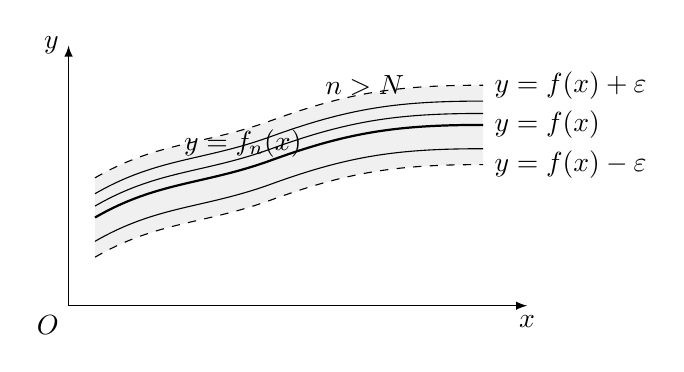
\begin{tikzpicture}[>=latex, scale=1.12]
    % 条形区域 f(x)-eps < y < f(x)+eps
    \fill[black!6] (0.4,1.00) to[out=30,in=200] (2.4,1.65) to[out=20,in=180] (4.80,2.05)
      -- (4.80,2.95) to[out=180,in=20] (2.4,2.55) to[out=200,in=30] (0.4,1.90) -- cycle;
    % 上、下边界（虚线）
    \draw[dashed] (0.4,1.90) to[out=30,in=200] (2.4,2.55) to[out=20,in=180] (4.80,2.95);
    \draw[dashed] (0.4,1.00) to[out=30,in=200] (2.4,1.65) to[out=20,in=180] (4.80,2.05);
    % 极限函数 y=f(x)
    \draw[thick] (0.4,1.45) to[out=30,in=200] (2.4,2.10) to[out=20,in=180] (4.80,2.50);
    % N 之后的曲线 y=f_n(x)
    \draw[thin] (0.4,1.18) to[out=30,in=200] (2.4,1.83) to[out=20,in=180] (4.80,2.23);
    \draw[thin] (0.4,1.58) to[out=30,in=200] (2.4,2.23) to[out=20,in=180] (4.80,2.63);
    \draw[thin] (0.4,1.72) to[out=30,in=200] (2.4,2.37) to[out=20,in=180] (4.80,2.77);
    % 坐标轴
    \draw[->] (0.10,0.45) -- (5.30,0.45) node[below] {$x$};
    \draw[->] (0.10,0.45) -- (0.10,3.40) node[left] {$y$};
    \node[below left] at (0.10,0.45) {$O$};
    % 文字标注
    \node[right] at (4.82,2.95) {$y=f(x)+\varepsilon$};
    \node[right] at (4.82,2.50) {$y=f(x)$};
    \node[right] at (4.82,2.05) {$y=f(x)-\varepsilon$};
    \node[above right] at (1.30,2.02) {$y=f_{n}(x)$};
    \node[above right] at (2.90,2.72) {$n>N$};
  \end{tikzpicture}
  \caption{一致收敛的几何意义}\label{fig:13.1.1}
\end{figure}

根据这个定义, 函数列 $\{x^{n}\}$ 在 $(0,1)$ 上收敛于 $0$, 但不一致收敛于 $0$. 从 \cref{fig:13.1.2} 可以看出, 不论 $n$ 多大, 曲线 $y=x^{n}$ 永远不会全部落入条形区域 $-\varepsilon<y<\varepsilon$ 之中, 其中 $\varepsilon\in(0,1)$. 因而 $\{x^{n}\}$ 在 $(0,1)$ 上不是一致收敛于 $0$ 的.

\begin{figure}[htbp]
  \centering
  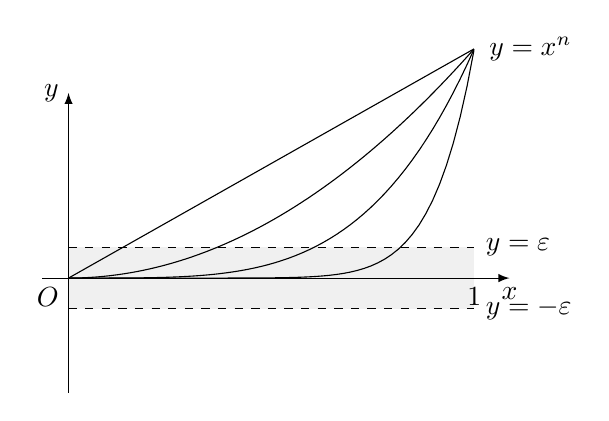
\begin{tikzpicture}[>=latex, scale=1.12]
    % 条形区域 -eps < y < eps
    \fill[black!6] (0,0.35) rectangle (4.60,-0.35);
    \draw[dashed] (0,0.35) -- (4.60,0.35);
    \draw[dashed] (0,-0.35) -- (4.60,-0.35);
    % 曲线 y=x^n (n=1,2,4,10)
    \foreach \n in {1,2,4,10}{
      \draw[thin, domain=0:1, samples=60] plot ({\x*4.60}, {pow(\x,\n)*2.60});
    }
    % 坐标轴
    \draw[->] (-0.30,0) -- (5.00,0) node[below] {$x$};
    \draw[->] (0,-1.30) -- (0,2.10) node[left] {$y$};
    \node[below left] at (0,0) {$O$};
    \node[below] at (4.60,0) {$1$};
    % 文字标注
    \node[right] at (4.62,0.35) {$y=\varepsilon$};
    \node[right] at (4.62,-0.35) {$y=-\varepsilon$};
    \node[right] at (4.66,2.60) {$y=x^{n}$};
  \end{tikzpicture}
  \caption{$\{x^{n}\}$ 在 $(0,1)$ 上不一致收敛}\label{fig:13.1.2}
\end{figure}

而由例~\ref{ex:13.1.8}(2) 的证明知, 函数列 $\left\{\frac{1}{n+x}\right\}$ 在 $(0,1)$ 上一致收敛于 $0$.

像数列的 Cauchy 收敛准则一样, 也有判断函数列是否一致收敛的 Cauchy 准则, 它的优点是无需知道极限函数, 就能判别其是否一致收敛.

\begin{theorem}[函数列一致收敛的 Cauchy 收敛准则]\label{thm:13.1.1}
设 $\{f_{n}(x)\}$ 为 $I\subset\mathbb{R}$ 上的一个函数列, 则以下结论等价:

(1) $\{f_{n}(x)\}$ 在 $I$ 上一致收敛;

(2) $\forall\varepsilon>0$, $\exists N=N(\varepsilon)\in\mathbb{N}$, 当 $n,m>N$ 时, $|f_{m}(x)-f_{n}(x)|<\varepsilon$, $\forall x\in I$;

(3) $\forall\varepsilon>0$, $\exists N=N(\varepsilon)\in\mathbb{N}$, 当 $n>N$ 时, $|f_{n+p}(x)-f_{n}(x)|<\varepsilon$, $\forall x\in I$, $\forall p\in\mathbb{N}$.
\end{theorem}

\begin{proof}
(2) $\Leftrightarrow$ (3) 显然.

(1) $\Rightarrow$ (2) 设 $\{f_{n}(x)\}$ 在 $I$ 上一致收敛于 $f(x)$, 则 $\forall\varepsilon>0$, $\exists N=N(\varepsilon)\in\mathbb{N}$, 当 $n>N$ 时, 有
\[
  |f_{n}(x)-f(x)|<\frac{\varepsilon}{2},\quad\forall x\in I.
\]
于是, 当 $n,m>N$ 时, 有
\[
  |f_{m}(x)-f_{n}(x)|\leqslant|f_{m}(x)-f(x)|+|f(x)-f_{n}(x)|<\frac{\varepsilon}{2}+\frac{\varepsilon}{2}=\varepsilon,\quad\forall x\in I.
\]

(1) $\Leftrightarrow$ (2) 设 (2) 成立, 则 $\forall\varepsilon>0$, $\exists N=N(\varepsilon)\in\mathbb{N}$, 当 $n,m>N$ 时, $|f_{m}(x)-f_{n}(x)|<\frac{\varepsilon}{2}$, $\forall x\in I$. 根据数列的 Cauchy 收敛准则, $\{f_{n}(x)\}$ 在 $I$ 上每点 $x$ 处都收敛, 设其极限函数为 $f(x)$. 在
\[
  |f_{m}(x)-f_{n}(x)|<\frac{\varepsilon}{2}
\]
中令 $m\to+\infty$ 得到
\[
  |f(x)-f_{n}(x)|\leqslant\frac{\varepsilon}{2}<\varepsilon,\quad\forall x\in I.
\]
根据定义~\ref{def:13.1.2}, $\{f_{n}(x)\}$ 在 $I$ 上一致收敛于 $f(x)$.
\end{proof}

\begin{theorem}\label{thm:13.1.2}
函数列 $\{f_{n}(x)\}$ 在 $I\subset\mathbb{R}$ 上一致收敛于 $f(x)$ $\Leftrightarrow$ $\lim\limits_{n\to+\infty}\beta_{n}=0$, 其中 $\beta_{n}=\sup\limits_{x\in I}|f_{n}(x)-f(x)|$.
\end{theorem}

\begin{proof}
($\Rightarrow$) 设 $\{f_{n}(x)\}$ 在 $I$ 上一致收敛, 则 $\forall\varepsilon>0$, $\exists N=N(\varepsilon)\in\mathbb{N}$, 当 $n>N$ 时, 有
\[
  |f_{n}(x)-f(x)|<\frac{\varepsilon}{2},\quad\forall x\in I.
\]
由此得到
\[
  \beta_{n}=\sup_{x\in I}|f_{n}(x)-f(x)|\leqslant\frac{\varepsilon}{2}<\varepsilon,
\]
即 $\lim\limits_{n\to+\infty}\beta_{n}=0$.

($\Leftrightarrow$) 设 $\lim\limits_{n\to+\infty}\beta_{n}=0$, 则 $\forall\varepsilon>0$, $\exists N=N(\varepsilon)\in\mathbb{N}$, 当 $n>N$ 时, $\beta_{n}<\varepsilon$. 有
\[
  |f_{n}(x)-f(x)|\leqslant\sup_{u\in I}|f_{n}(u)-f(u)|\doteq\beta_{n}<\varepsilon,
\]
这就证明了 $\{f_{n}(x)\}$ 在 $I$ 上是一致收敛的.
\end{proof}

\begin{example}\label{ex:13.1.9}
在例~\ref{ex:13.1.8}(1) 中, 由于
\[
  \beta_{n}=\sup_{x\in(0,1)}|f_{n}(x)-f(x)|=\sup_{x\in(0,1)}x^{n}=1\not\to0\quad(n\to+\infty),
\]
故 $f_{n}(x)=x^{n}$ 在 $(0,1)$ 上不一致收敛.
\end{example}

\begin{example}\label{ex:13.1.10}
分别讨论函数列 $f_{n}(x)=\frac{nx}{1+n^{2}x^{2}}$ 在 $(0,1)$ 与 $(1,+\infty)$ 上的一致收敛性.
\end{example}

\begin{proof}
对任意给定的 $x\in(0,+\infty)$, 显然, $f(x)=\lim\limits_{n\to+\infty}f_{n}(x)=\lim\limits_{n\to+\infty}\frac{nx}{1+n^{2}x^{2}}=0$.

(1) 当 $x\in(0,1)$ 时, 由于
\[
  \beta_{n}=\sup_{x\in(0,1)}|f_{n}(x)-f(x)|=\left|f_{n}\left(\frac{1}{n}\right)-f\left(\frac{1}{n}\right)\right|=\frac{1}{2}\not\to0\quad(n\to+\infty),
\]
所以, $\lim\limits_{n\to+\infty}\beta_{n}\neq0$. 根据定理~\ref{thm:13.1.2} 知, $\{f_{n}(x)\}$ 在 $(0,1)$ 上不一致收敛于 $0$.

(2) 当 $x\in(1,+\infty)$ 时, $\forall\varepsilon>0$, 取 $N=N(\varepsilon)>\frac{1}{\varepsilon}$, 当 $n>N$ 时, 有
\[
  |f_{n}(x)-f(x)|=\frac{nx}{1+n^{2}x^{2}}\leqslant\frac{nx}{n^{2}x^{2}}=\frac{1}{nx}<\frac{1}{n}<\frac{1}{N}<\varepsilon,
\]
故 $\{f_{n}(x)\}$ 在 $(1,+\infty)$ 上一致收敛于 $0$. 或者由
\[
  0\leqslant\beta_{n}=\sup_{x\in(1,+\infty)}|f_{n}(x)-f(x)|\leqslant\frac{1}{n}\to0\quad(n\to+\infty)
\]
及夹逼定理得到 $\lim\limits_{n\to+\infty}\beta_{n}=0$. 根据定理~\ref{thm:13.1.2} 知 $\{f_{n}(x)\}$ 在 $(1,+\infty)$ 上一致收敛.
\end{proof}

\begin{example}\label{ex:13.1.11}
讨论函数列
\[
  f_{n}(x)=2n^{2}x\mathrm{e}^{-n^{2}x^{2}},\quad n=1,2,\cdots
\]
在 $[0,1]$ 上的一致收敛性.
\end{example}

\begin{proof}
从例~\ref{ex:13.1.4} 知, $f(x)=\lim\limits_{n\to+\infty}f_{n}(x)=\lim\limits_{n\to+\infty}2n^{2}x\mathrm{e}^{-n^{2}x^{2}}=0$. 由于
\[
  \beta_{n}=\sup_{x\in(0,1)}|f_{n}(x)-f(x)|\geqslant\left|f_{n}\left(\frac{1}{n}\right)-f\left(\frac{1}{n}\right)\right|=2n\mathrm{e}^{-1}\to+\infty\neq0\quad(n\to+\infty),
\]
故 $\lim\limits_{n\to+\infty}\beta_{n}\neq0$. 根据定理~\ref{thm:13.1.2} 推得 $\{f_{n}(x)\}$ 在 $[0,1]$ 上非一致收敛.
\end{proof}

\begin{example}\label{ex:13.1.12}
证明:
\[
  \sum_{n=1}^{\infty}\bigl[\mathrm{e}^{-n^{2}x^{2}}-\mathrm{e}^{-(n-1)^{2}x^{2}}\bigr]
\]
在 $(0,1)$ 中不一致收敛.
\end{example}

\begin{proof}
$S_{n}(x)=\mathrm{e}^{-n^{2}x^{2}}-1$,
\[
  S(x)=\lim_{n\to+\infty}(\mathrm{e}^{-n^{2}x^{2}}-1)=0-1=-1,\quad\forall x\in(0,1).
\]
\[
  \begin{aligned}
    \beta_{n}&=\sup_{x\in(0,1)}|S_{n}(x)-S(x)|=\sup_{x\in(0,1)}\mathrm{e}^{-n^{2}x^{2}}\geqslant\mathrm{e}^{-n^{2}\cdot\frac{1}{n^{2}}}\\
    &=\mathrm{e}^{-1}\not\to0\quad(n\to+\infty),
  \end{aligned}
\]
从而 $\lim\limits_{n\to+\infty}\beta_{n}\neq0$. 根据定理~\ref{thm:13.1.2}, 原函数项级数在 $(0,1)$ 中不一致收敛.
\end{proof}

%  第二部分：定义 13.1.2' 起（生成脚本 tools/_make_ch13_1b.py）
% ==================================================================

% ===== PART-B =====

应用函数项级数与部分和函数列之间的对偶关系, 我们将给出函数项级数的一致收敛及其判别法.

\begin{definitionp}\label{def:13.1.2p}
设 $\sum_{n=1}^{\infty}u_{n}(x)$ 是定义在 $I\subset\mathbb{R}$ 上的函数项级数, $S_{n}(x)=\sum_{k=1}^{n}u_{k}(x)$ 为其部分和. 如果函数列 $\{S_{n}(x)\}$ 在 $I$ 上一致收敛于 $S(x)$, 就称 $\sum_{n=1}^{\infty}u_{n}(x)$ 在 $I$ 上一致收敛于 $S(x)$. 并记 $S(x)=\sum_{n=1}^{\infty}u_{n}(x)$. 用 $\varepsilon$-$N$ 语言表达为: $\forall\varepsilon>0$, $\exists N=N(\varepsilon)\in\mathbb{N}$, 当 $n>N$ 时, 有
\[
  \left|\sum_{k=n+1}^{\infty}u_{k}(x)\right|=\left|\sum_{k=1}^{n}u_{k}(x)-\sum_{k=1}^{\infty}u_{k}(x)\right|=|S_{n}(x)-S(x)|<\varepsilon,\quad\forall x\in I.
\]
\end{definitionp}

% 定理 13.1.1' 排在定理 13.1.2 之后：先把计数器拨回 1（环境内 -1 再自增 -> 13.1.1'），
% 退出后再拨回 2，使下一个普通定理为 13.1.3。
\setcounter{theorem}{1}
\begin{theoremp}[函数项级数一致收敛的 Cauchy 准则]\label{thm:13.1.1p}
以下结论等价:

(1) 函数项级数 $\sum_{n=1}^{\infty}u_{n}(x)$ 在 $I\subset\mathbb{R}$ 上一致收敛;

(2) $\forall\varepsilon>0$, $\exists N=N(\varepsilon)\in\mathbb{N}$, 当 $m>n>N$ 时, 有
\[
  \left|\sum_{k=n+1}^{m}u_{k}(x)\right|<\varepsilon,\quad\forall x\in I;
\]

(3) $\forall\varepsilon>0$, $\exists N=N(\varepsilon)\in\mathbb{N}$, 当 $n>N$ 时, 有
\[
  \left|\sum_{k=n+1}^{n+p}u_{k}(x)\right|<\varepsilon,\quad\forall p\in\mathbb{N},\quad\forall x\in I.
\]
\end{theoremp}
\addtocounter{theorem}{1}

\begin{proof}
(1)
\[
  \begin{aligned}
    &\sum_{n=1}^{\infty}u_{n}(x)\text{ 在 }I\text{ 上一致收敛}\\
    &\Leftrightarrow\{S_{n}(x)\}\text{ 在 }I\text{ 上一致收敛}\\
    &\Leftrightarrow\forall\varepsilon>0,\ \exists N=N(\varepsilon)\in\mathbb{N},\ \text{当 }m\geqslant n>N\text{ 时, 有}\\
    &\qquad|S_{m}(x)-S_{n}(x)|<\varepsilon,\quad\forall x\in I\\
    &\Leftrightarrow(2)\ \forall\varepsilon>0,\ \exists N=N(\varepsilon)\in\mathbb{N},\ \text{当 }m>n>N\text{ 时, 有}\\
    &\qquad\left|\sum_{k=n+1}^{m}u_{k}(x)\right|=\left|\sum_{k=1}^{m}u_{k}(x)-\sum_{k=1}^{n}u_{k}(x)\right|<\varepsilon,\quad\forall x\in I.
  \end{aligned}
\]

(2) $\Leftrightarrow$ (3) 显然.
\end{proof}

\begin{corollary}[函数项级数一致收敛的必要条件]\label{cor:13.1.1}
函数项级数 $\sum_{n=1}^{\infty}u_{n}(x)$ 在 $I\subset\mathbb{R}$ 上一致收敛的必要条件是通项 $u_{n}(x)\rightrightarrows0$, $x\in I$ ($n\to+\infty$). 但反之不真.
\end{corollary}

\begin{proof}
证法 1 由定理~\ref{thm:13.1.1p}(3) 中取 $p=1$ 立知, $\forall\varepsilon>0$, $\exists N=N(\varepsilon)\in\mathbb{N}$, 当 $n>N$ 时, 有
\[
  |u_{n+1}(x)|=\left|\sum_{k=n+1}^{n+1}u_{k}(x)\right|<\varepsilon,\quad\forall x\in I.
\]
于是, $u_{n}(x)\rightrightarrows0$, $x\in I$ ($n\to+\infty$).

但反之不真. 反例: $u_{n}(x)=\frac{1}{n}$.

证法 2 因为 $\sum_{n=1}^{\infty}u_{n}(x)$ 在 $I$ 上一致收敛, 所以 $\{S_{n}(x)\}$ 在 $I$ 上一致收敛, 即 $\forall\varepsilon>0$, $\exists N=N(\varepsilon)\in\mathbb{N}$, 当 $n>N$ 时, 有
\[
  |S_{n}(x)-S(x)|<\frac{\varepsilon}{2},\quad\forall x\in I.
\]
于是, 当 $n>N+1$ 时, 有
\[
  \begin{aligned}
    |u_{n}(x)|&=|S_{n}(x)-S_{n-1}(x)|\leqslant|S_{n}(x)-S(x)|+|S(x)-S_{n-1}(x)|\\
    &<\frac{\varepsilon}{2}+\frac{\varepsilon}{2}=\varepsilon,\quad\forall x\in I.
  \end{aligned}
\]
这就证明了 $u_{n}(x)\rightrightarrows0$, $x\in I$ ($n\to+\infty$).
\end{proof}

这个必要条件经常用来判断函数项级数的非一致收敛性, 即如果 $u_{n}(x)\not\rightrightarrows0$, $x\in I$ ($n\to+\infty$), 则函数项级数 $\sum_{n=1}^{\infty}u_{n}(x)$ 在 $I$ 上非一致收敛. 它由局部 ($u_{n}(x)$) 的性态反映了整体 $\left(\sum_{n=1}^{\infty}u_{n}(x)\right)$ 的性态.

下面的 Weierstrass 判别法是判别函数项级数一致收敛的最常用也是最简单的方法. 读者在讨论函数项级数的一致收敛性时, 它是首选的判别法, 切记!

\begin{theorem}[Weierstrass 判别法]\label{thm:13.1.3}
如果存在收敛的正项级数 $\sum_{n=1}^{\infty}a_{n}$, 使得
\[
  |u_{n}(x)|\leqslant a_{n},\quad n=1,2,\cdots,\ \forall x\in I\subset\mathbb{R},
\]
则函数项级数 $\sum_{n=1}^{\infty}u_{n}(x)$ 在 $I$ 上一致收敛. 而数项级数 $\sum_{n=1}^{\infty}a_{n}$ 称为 $\sum_{n=1}^{\infty}u_{n}(x)$ 在 $I$ 上的优级数.
\end{theorem}

\begin{proof}
因为正项级数 $\sum_{n=1}^{\infty}a_{n}$ 收敛, 由数项级数的 Cauchy 收敛准则, $\forall\varepsilon>0$, $\exists N=N(\varepsilon)\in\mathbb{N}$, 当 $n>N$ 时, 有
\[
  a_{n+1}+\cdots+a_{n+p}<\varepsilon,\quad\forall p\in\mathbb{N}.
\]
由题设 $|u_{n}(x)|\leqslant a_{n}$ ($n=1,2,\cdots$) 知道, 当 $n>N$ 时, 有
\[
  \Big|\sum_{k=n+1}^{n+p}u_{k}(x)\Big|\leqslant\sum_{k=n+1}^{n+p}|u_{k}(x)|\leqslant\sum_{k=n+1}^{n+p}a_{k}<\varepsilon,\quad\forall p\in\mathbb{N},\ \forall x\in I.
\]
则根据函数项级数一致收敛的 Cauchy 准则 (定理~\ref{thm:13.1.1p}), $\sum_{n=1}^{\infty}u_{n}(x)$ 在 $I$ 上是一致收敛的.
\end{proof}

\begin{remark}\label{rem:13.1.1}
如果定理~\ref{thm:13.1.3} 中收敛的正项级数, 改为更一般的一致收敛的正项级数 $\sum_{n=1}^{\infty}a_{n}(x)$, $|u_{n}(x)|\leqslant a_{n}(x)$ ($n=1,2,\cdots$), 则 $\sum_{n=1}^{\infty}u_{n}(x)$ 在 $I$ 上一致收敛的结论依然成立. 其证明与定理~\ref{thm:13.1.3} 完全类似.
\end{remark}

\begin{example}\label{ex:13.1.13}
证明: 函数项级数 $\sum_{n=1}^{\infty}n\mathrm{e}^{-nx}$

(1) 在 $[\delta,+\infty)$ ($\delta>0$) 上一致收敛;

(2) 在 $(0,+\infty)$ 上非一致收敛.
\end{example}

\begin{proof}
证法 1 (1) 由于 $x\geqslant\delta>0$, 故必 $\exists N\in\mathbb{N}$, 当 $n>N$ 时, 有
\[
  0<n\mathrm{e}^{-nx}\leqslant n\mathrm{e}^{-n\delta}<\frac{1}{n^{2}}.
\]
又因 $\sum_{n=1}^{\infty}\frac{1}{n^{2}}$ 收敛, 根据 Weierstrass 判别法知, $\sum_{n=1}^{\infty}n\mathrm{e}^{-nx}$ 在 $[\delta,+\infty)$ 上一致收敛.

(2) 该函数项级数的通项为 $u_{n}(x)=n\mathrm{e}^{-nx}$. 由于 $\lim\limits_{n\to+\infty}u_{n}(x)=0$, $\forall x\in(0,+\infty)$, 故
\[
  \sup_{x\in(0,+\infty)}|u_{n}(x)-0|=\sup_{x\in(0,+\infty)}|u_{n}(x)|\geqslant u_{n}\left(\frac{1}{n}\right)=n\mathrm{e}^{-1}\to+\infty\neq0\quad(n\to+\infty),
\]
即 $u_{n}(x)\not\rightrightarrows0$, $x\in(0,+\infty)$ ($n\to+\infty$). 根据推论~\ref{cor:13.1.1}, $\sum_{n=1}^{\infty}n\mathrm{e}^{-nx}$ 在 $(0,+\infty)$ 上非一致收敛.

证法 2 (1) 因为 $0\leqslant n\mathrm{e}^{-nx}\leqslant n\mathrm{e}^{-n\delta}=\frac{n}{(\mathrm{e}^{\delta})^{n}}$, $\forall x\in[\delta,+\infty)$, 而由
\[
  \sqrt[n]{\frac{n}{(\mathrm{e}^{\delta})^{n}}}=\frac{\sqrt[n]{n}}{\mathrm{e}^{\delta}}\to\frac{1}{\mathrm{e}^{\delta}}<1
\]
及数项级数的 Cauchy 判别法知, $\sum_{n=1}^{\infty}n\mathrm{e}^{-n\delta}$ 收敛. 再由 Weierstrass 判别法, $\sum_{n=1}^{\infty}n\mathrm{e}^{-nx}$ 在 $[\delta,+\infty)$ ($\delta>0$) 内一致收敛.

(2) (反证) 假设 $\sum_{n=1}^{\infty}n\mathrm{e}^{-nx}$ 在 $(0,+\infty)$ 中一致收敛, 根据定理~\ref{thm:13.2.1} 知
\[
  \lim_{x\to0^{+}}\sum_{n=1}^{\infty}n\mathrm{e}^{-nx}\xlongequal{\text{逐项取极限}}\sum_{n=1}^{\infty}\lim_{x\to0^{+}}n\mathrm{e}^{-nx}=\sum_{n=1}^{\infty}n
\]
收敛, 这与 $\sum_{n=1}^{\infty}n=+\infty$ 发散相矛盾.
\end{proof}

\begin{example}\label{ex:13.1.14}
证明: 函数项级数

(1) $\sum_{n=1}^{\infty}\frac{\cos nx}{n^{2}}$ 在 $(-\infty,+\infty)$ 上一致收敛;

(2) $\sum_{n=1}^{\infty}\frac{x}{1+n^{4}x^{2}}$ 在 $[0,+\infty)$ 上一致收敛.
\end{example}

\begin{proof}
(1) 因为
\[
  |u_{n}(x)|=\left|\frac{\cos nx}{n^{2}}\right|\leqslant\frac{1}{n^{2}}
\]
及 $\sum_{n=1}^{\infty}\frac{1}{n^{2}}$ 收敛, 所以根据 Weierstrass 判别法, $\sum_{n=1}^{\infty}\frac{\cos nx}{n^{2}}$ 在 $(-\infty,+\infty)$ 上一致收敛.

(2) 因为 $2n^{2}x\leqslant1+n^{4}x^{2}$, $\forall x\in[0,+\infty)$, 所以
\[
  \frac{x}{1+n^{4}x^{2}}\leqslant\frac{1}{2n^{2}},\quad\forall x\in[0,+\infty).
\]
又因 $\sum_{n=1}^{\infty}\frac{1}{2n^{2}}$ 收敛, 根据 Weierstrass 判别法, $\sum_{n=1}^{\infty}\frac{x}{1+n^{4}x^{2}}$ 在 $[0,+\infty)$ 上一致收敛.
\end{proof}

\begin{example}\label{ex:13.1.15}
证明: $\sum_{n=1}^{\infty}x^{2}\mathrm{e}^{-nx}$ 在 $[0,+\infty)$ 中一致收敛.
\end{example}

\begin{proof}
设 $u_{n}(x)=x^{2}\mathrm{e}^{-nx}$, 则
\[
  u_{n}'(x)=2x\mathrm{e}^{-nx}-nx^{2}\mathrm{e}^{-nx}=x(2-nx)\mathrm{e}^{-nx}\begin{cases}
    >0, & x<\frac{2}{n},\ u_{n}(x)\nearrow,\\
    =0, & x=\frac{2}{n},\ u_{n}(x)\text{ 达最大值},\\
    <0, & x>\frac{2}{n},\ u_{n}(x)\searrow.
\end{cases}
\]
当 $x=\frac{2}{n}$ 时, $u_{n}(x)$ 在 $[0,+\infty)$ 中达到最大值. 于是
\[
  |u_{n}(x)|\leqslant\left|u_{n}\left(\frac{2}{n}\right)\right|=\left|\left(\frac{2}{n}\right)^{2}\mathrm{e}^{-n\cdot\frac{2}{n}}\right|=\frac{4}{\mathrm{e}^{2}}\frac{1}{n^{2}}.
\]
又因为 $\sum_{n=1}^{\infty}\frac{4}{\mathrm{e}^{2}}\frac{1}{n^{2}}$ 收敛, 根据 Weierstrass 判别法知, $\sum_{n=1}^{\infty}u_{n}(x)=\sum_{n=1}^{\infty}x^{2}\mathrm{e}^{-nx}$ 在 $[0,+\infty)$ 上一致收敛.
\end{proof}

Weierstrass 判别法用起来很方便, 但条件太强, 它要求函数项级数 $\sum_{n=1}^{\infty}u_{n}(x)$ 绝对收敛, 而且 $\sum_{n=1}^{\infty}u_{n}(x)$ 与 $\sum_{n=1}^{\infty}|u_{n}(x)|$ 在 $I$ 上都一致收敛. 实际上存在这样的函数项级数, 它一致收敛 (见例~\ref{ex:13.1.16}); 还有可能 $\sum_{n=1}^{\infty}u_{n}(x)$ 绝对且一致收敛, 但 $\sum_{n=1}^{\infty}|u_{n}(x)|$ 却不一致收敛 (见例~\ref{ex:13.1.17}). 对于这种级数 Weierstrass 判别法就无效了. 因此, 还需研究更精细的判别法.

类似于数项级数的 Dirichlet 与 Abel 判别法, 我们有函数项级数的 Dirichlet 与 Abel 判别法.

\begin{theorem}[Dirichlet 判别法]\label{thm:13.1.4}
如果函数项级数 $\sum_{n=1}^{\infty}a_{n}(x)b_{n}(x)$ 满足:

(1) $\{b_{n}(x)\}$ 对于每个固定的 $x\in I\subset\mathbb{R}$ 都是单调的, 且在 $I$ 上一致收敛于 $0$;

(2) $\sum_{n=1}^{\infty}a_{n}(x)$ 的部分和在 $I$ 上一致有界, 即
\[
  \left|\sum_{k=1}^{n}a_{k}(x)\right|\leqslant M,\quad\forall x\in I,\ n=1,2,\cdots,
\]
则 $\sum_{n=1}^{\infty}a_{n}(x)b_{n}(x)$ 在 $I$ 上一致收敛.
\end{theorem}

\begin{proof}
证法 1 类似定理~\ref{thm:12.3.2} 证法 1, 有
\[
  \left|\sum_{k=n+1}^{n+p}a_{k}(x)b_{k}(x)\right|\leqslant2M|b_{n+1}(x)|.
\]
因为 $\{b_{n}(x)\}$ 对于每个固定的 $x\in I\subset\mathbb{R}$ 都单调, 且一致收敛于 $0$, 所以 $\forall\varepsilon>0$, $\exists N\in\mathbb{N}$, 当 $n>N$ 时, $|b_{n+1}(x)|<\frac{\varepsilon}{2M+1}$, 从而
\[
  \left|\sum_{k=n+1}^{n+p}a_{k}(x)b_{k}(x)\right|<2M\cdot\frac{\varepsilon}{2M+1}<\varepsilon,\quad\forall p\in\mathbb{N}.
\]
根据函数项级数一致收敛准则 (定理~\ref{thm:13.1.1p}), $\sum_{n=1}^{\infty}a_{n}(x)b_{n}(x)$ 在 $I$ 上一致收敛.

证法 2 由 (2), $\{b_{n}(x)\}$ 单调及 Abel 引理~\ref{lem:12.3.2}(2) 知
\[
  \begin{aligned}
    \Big|\sum_{k=n+1}^{n+p}a_{k}(x)\Big|&=|S_{n+p}(x)-S_{n}(x)|\leqslant|S_{n+p}(x)|+|S_{n}(x)|\leqslant2M,\\
    \Big|\sum_{k=n+1}^{n+p}a_{k}(x)b_{k}(x)\Big|&\leqslant2M(|b_{n+1}(x)|+2|b_{n+p}(x)|).
  \end{aligned}
\]
因为 $\{b_{n}(x)\}$ 在 $I$ 上一致收敛于 $0$, 所以 $\forall\varepsilon>0$, $\exists N=N(\varepsilon)\in\mathbb{N}$, 当 $n>N$ 时, $|b_{n}(x)|<\frac{\varepsilon}{6M+1}$, $\forall x\in I$. 于是
\[
  \left|\sum_{k=n+1}^{n+p}a_{k}(x)b_{k}(x)\right|\leqslant2M(|b_{n+1}(x)|+2|b_{n+p}(x)|)<2M\cdot\frac{3\varepsilon}{6M+1}<\varepsilon,
\]
\[
  \forall x\in I,\ \forall p\in\mathbb{N}.
\]
根据函数项级数的一致收敛 Cauchy 收敛准则 (定理~\ref{thm:13.1.1p}), $\sum_{n=1}^{\infty}a_{n}(x)b_{n}(x)$ 在 $I$ 上一致收敛.
\end{proof}

\begin{theorem}[Abel 判别法]\label{thm:13.1.5}
如果函数项级数 $\sum_{n=1}^{\infty}a_{n}(x)b_{n}(x)$ 满足:

(1) $\{b_{n}(x)\}$ 对于每个固定的 $x\in I\subset\mathbb{R}$ 都是单调的, 并且在 $I$ 上一致有界, 即 $|b_{n}(x)|\leqslant B$, $\forall x\in I$, $\forall n\in\mathbb{N}$.

(2) 函数项级数 $\sum_{n=1}^{\infty}a_{n}(x)$ 在 $I$ 上一致收敛.

则 $\sum_{n=1}^{\infty}a_{n}(x)b_{n}(x)$ 在 $I$ 上一致收敛.
\end{theorem}

\begin{proof}
证法 1 由条件 $|b_{n}(x)|\leqslant B$, $\forall n\in\mathbb{N}$. 又因为 $\sum_{n=1}^{\infty}a_{n}(x)$ 在 $I$ 上一致收敛, 故 $\forall\varepsilon>0$ 根据函数项级数的一致收敛 Cauchy 收敛准则 (定理~\ref{thm:13.1.1p}), $\exists N=N(\varepsilon)\in\mathbb{N}$, 当 $n>N$ 时, 有
\[
  \left|\sum_{k=n+1}^{n+p}a_{k}(x)\right|<\frac{\varepsilon}{2B+1},\quad\forall x\in I,\ \forall p\in\mathbb{N}.
\]
于是, $\sum_{k=n+1}^{n+p}a_{k}(x)$ 在 $I$ 上一致有界. 类似定理~\ref{thm:12.3.3} 证法 2, 有
\[
  \left|\sum_{k=n+1}^{n+p}a_{k}(x)b_{k}(x)\right|\leqslant\frac{\varepsilon}{2B+1}|b_{n+1}(x)|<\frac{\varepsilon}{2B+1}\cdot B<\varepsilon,\quad\forall x\in I,\ \forall p\in\mathbb{N}.
\]
再从函数项级数的一致收敛 Cauchy 收敛准则 (定理~\ref{thm:13.1.1p}), $\sum_{n=1}^{\infty}a_{n}(x)b_{n}(x)$ 在 $I$ 上一致收敛.

证法 2 由条件 $|b_{n}(x)|\leqslant B$, $\forall x\in I$, $\forall n\in\mathbb{N}$. 又因 $\sum_{n=1}^{\infty}a_{n}(x)$ 在 $I$ 上一致收敛, 故 $\forall\varepsilon>0$, 根据函数项级数的一致收敛 Cauchy 收敛准则 (定理~\ref{thm:13.1.1p}), $\exists N=N(\varepsilon)\in\mathbb{N}$, 当 $n>N$ 时, 有
\[
  \left|\sum_{k=n+1}^{n+p}a_{k}(x)\right|<\frac{\varepsilon}{3B+1},\quad\forall x\in I,\ \forall p\in\mathbb{N}.
\]
于是, 根据 Abel 引理~\ref{lem:12.3.2}(2) 得到
\[
  \begin{aligned}
    \left|\sum_{k=n+1}^{n+p}a_{k}(x)b_{k}(x)\right|&\leqslant\frac{\varepsilon}{3B+1}(|b_{n+1}(x)|+2|b_{n+p}(x)|)\\
    &\leqslant\frac{\varepsilon}{3B+1}\cdot3B<\varepsilon,\quad\forall x\in I,\ \forall p\in\mathbb{N}.
  \end{aligned}
\]
再从函数项级数一致收敛的 Cauchy 收敛准则 (定理~\ref{thm:13.1.1p}) 得 $\sum_{n=1}^{\infty}a_{n}(x)b_{n}(x)$ 在 $I$ 上一致收敛.
\end{proof}

\begin{remark}\label{rem:13.1.2}
(1) 定理~\ref{thm:12.3.3} 证法 1 不能类推出定理~\ref{thm:13.1.5}. 这是因为不能证明 $b_{n}'(x)=b_{n}(x)-b(x)$ 一致收敛于 $0$.

(2) 显然, Dirichlet 判别法的条件 (1) 强于 Abel 判别法的条件 (1), 而 Dirichlet 判别法的条件 (2) 弱于 Abel 判别法的条件 (2), 它们各有千秋. 但其结论是完全相同的.
\end{remark}

\begin{example}\label{ex:13.1.16}
证明: 函数项级数 $\sum_{n=1}^{\infty}\frac{\cos nx}{n}$

(1) 在 $[\delta,2\pi-\delta]$ ($0<\delta<\pi$) 上一致收敛;

(2) 在 $(0,2\pi)$ 中不一致收敛.
\end{example}

\begin{proof}
(1) $b_{n}(x)=\frac{1}{n}$ 单调减一致收敛于 $0$. 设 $a_{n}(x)=\cos nx$, 当 $x\in[\delta,2\pi-\delta]$ ($0<\delta<\pi$) 时, $\left|\sin\frac{x}{2}\right|\geqslant\sin\frac{\delta}{2}$, 所以
\[
  \left|\sum_{k=1}^{n}\cos kx\right|=\left|\frac{\sin\left(n+\frac{1}{2}\right)x-\sin\frac{x}{2}}{2\sin\frac{x}{2}}\right|\leqslant\frac{1}{\left|\sin\frac{x}{2}\right|}\leqslant\frac{1}{\sin\frac{\delta}{2}},
\]
即 $\left|\sum_{k=1}^{n}\cos kx\right|$ 在 $[\delta,2\pi-\delta]$ 中一致有界. 根据 Dirichlet 判别法知, 原级数在 $[\delta,2\pi-\delta]$ 中一致收敛.

(2) 方法 1. (反证) 假设 $\sum_{n=1}^{\infty}\frac{\cos nx}{n}$ 在 $(0,2\pi)$ 中一致收敛, 则 $\forall\varepsilon>0$, $\exists N=N(\varepsilon)\in\mathbb{N}$, 当 $n>N$ 时, 有
\[
  \left|\frac{\cos(n+1)x}{n+1}+\cdots+\frac{\cos(n+p)x}{n+p}\right|<\varepsilon,\quad\forall x\in(0,2\pi),\ \forall p\in\mathbb{N}.
\]
今取 $p=n$, $x=\frac{\pi}{8n}$, $\varepsilon=\frac{\sqrt{2}}{4}$, 则有
\[
  \frac{\sqrt{2}}{4}=\varepsilon>\left|\frac{\cos(n+1)\frac{\pi}{8n}}{n+1}+\cdots+\frac{\cos2n\cdot\frac{\pi}{8n}}{2n}\right|>\frac{\cos\frac{\pi}{4}}{2n}\cdot n=\frac{\sqrt{2}}{4},
\]
矛盾. 因此, $\sum_{n=1}^{\infty}\frac{\cos nx}{n}$ 在 $(0,2\pi)$ 中不一致收敛.

方法 2. (反证) 假设 $\sum_{n=1}^{\infty}\frac{\cos nx}{n}$ 在 $(0,2\pi)$ 中一致收敛, 根据下面逐项求极限的定理~\ref{thm:13.2.1} 知
\[
  \lim_{x\to0}\sum_{n=1}^{\infty}\frac{\cos nx}{n}=\sum_{n=1}^{\infty}\lim_{x\to0}\frac{\cos nx}{n}=\sum_{n=1}^{\infty}\frac{1}{n}
\]
收敛, 这与已证得 $\sum_{n=1}^{\infty}\frac{1}{n}$ 发散相矛盾.
\end{proof}

\begin{example}\label{ex:13.1.17}
证明: 函数项级数 $\sum_{n=1}^{\infty}\frac{\sin nx}{n}$

(1) 在 $[\delta,2\pi-\delta]$ ($0<\delta<\pi$) 上一致收敛;

(2) 在 $(0,2\pi)$ 中不一致收敛.
\end{example}

\begin{proof}
(1) $b_{n}(x)=\frac{1}{n}$ 单调减一致收敛于 $0$. 设 $a_{n}=\sin nx$, 当 $x\in[\delta,2\pi-\delta]$ ($0<\delta<\pi$) 时, $\left|\sin\frac{x}{2}\right|\geqslant\sin\frac{\delta}{2}$, 所以
\[
  \left|\sum_{k=1}^{n}\sin kx\right|=\frac{\left|\cos\left(n+\frac{1}{2}\right)x-\cos\frac{x}{2}\right|}{2\sin\frac{x}{2}}\leqslant\frac{1}{\sin\frac{x}{2}}<\frac{1}{\sin\frac{\delta}{2}},
\]
即 $\left|\sum_{k=1}^{n}\sin kx\right|$ 在 $[\delta,2\pi-\delta]$ 中一致有界. 根据 Dirichlet 判别法知, 原级数在 $[\delta,2\pi-\delta]$ 中一致收敛.

(2) (反证) 假设 $\sum_{n=1}^{\infty}\frac{\sin nx}{n}$ 在 $(0,2\pi)$ 中一致收敛, 则 $\forall\varepsilon>0$, $\exists N=N(\varepsilon)\in\mathbb{N}$, 当 $n>N$ 时, 有
\[
  \left|\frac{\sin(n+1)x}{n+1}+\cdots+\frac{\sin(n+p)x}{n+p}\right|<\varepsilon,\quad\forall x\in(0,2\pi),\ \forall p\in\mathbb{N}.
\]
今取 $p=n$, $x=\frac{\pi}{4(n+1)}$, $\varepsilon=\frac{\sqrt{2}}{4}$, 则有
\[
  \begin{aligned}
    &\frac{\sqrt{2}}{4}=\varepsilon>\left|\frac{\sin(n+1)\cdot\frac{\pi}{4(n+1)}}{n+1}+\cdots+\frac{\sin2n\cdot\frac{\pi}{4(n+1)}}{2n}\right|\\
    &\geqslant\frac{\sin\frac{\pi}{4}}{2n}\cdot n=\frac{\sqrt{2}}{4},
  \end{aligned}
\]
矛盾. 因此, $\sum_{n=1}^{\infty}\frac{\sin nx}{n}$ 在 $(0,2\pi)$ 中不一致收敛.
\end{proof}

关于一致收敛, 下面例子的证明方法很值得回味.

\begin{example}\label{ex:13.1.18}
设 $\{a_{n}\}$ 为单调减的非负数列. 证明: 函数项级数 $\sum_{n=1}^{\infty}a_{n}\sin nx$ 在 $(-\infty,+\infty)$ 上一致收敛 $\Leftrightarrow$ $\lim\limits_{n\to+\infty}na_{n}=0$, 即 $a_{n}=o\left(\frac{1}{n}\right)$, $n\to+\infty$.
\end{example}

\begin{proof}
($\Rightarrow$) 设 $\sum_{n=1}^{\infty}a_{n}\sin nx$ 在 $(-\infty,+\infty)$ 上一致收敛, 则 $\forall\varepsilon>0$, $\exists N=N(\varepsilon)\in\mathbb{N}$, 当 $m>n>N$ 时, 有
\[
  \left|\sum_{k=n}^{m}a_{k}\sin kx\right|<\varepsilon,\quad\forall x\in(-\infty,+\infty).
\]
今取 $m\geqslant2N$, $n=\left[\frac{m}{2}+1\right]$, 则 $n\leqslant\frac{m}{2}+1<n+1$, 即 $n>\frac{m}{2}>N$. 再取 $x=\frac{\pi}{2m}$, 有
\[
  \left|\sum_{k=n}^{m}a_{k}\sin k\frac{\pi}{2m}\right|<\varepsilon.
\]
当 $n\leqslant k\leqslant m$ 时, $\frac{\pi}{4}<\frac{n}{m}\frac{\pi}{2}\leqslant k\frac{\pi}{2m}\leqslant\frac{\pi}{2}$, 所以
\[
  \sin k\frac{\pi}{2m}\geqslant\sin\frac{\pi}{4}=\frac{\sqrt{2}}{2}.
\]
于是
\[
  \varepsilon>\sum_{k=n}^{m}a_{k}\sin k\frac{\pi}{2m}\geqslant\frac{\sqrt{2}}{2}\sum_{k=n}^{m}a_{k}\geqslant(m-n+1)a_{m}\frac{\sqrt{2}}{2}\geqslant\frac{\sqrt{2}}{4}ma_{m}\geqslant0,
\]
即
\[
  \lim_{n\to+\infty}na_{n}=\lim_{m\to+\infty}ma_{m}=0.
\]

($\Leftrightarrow$) 设 $\lim\limits_{n\to+\infty}na_{n}=0$. 令
\[
  \mu_{n}=\sup_{m\geqslant n}\{ma_{m}\},
\]
则 $\{\mu_{n}\}$ 单调减少趋于 $0$. 对于 $m\geqslant n$, 记
\[
  S_{n,m}(x)=\sum_{k=n}^{m}a_{k}\sin kx.
\]
下面证明
\[
  |S_{n,m}(x)|\leqslant(\pi+3)\mu_{n},\quad\forall x\in(-\infty,+\infty).
\]
再由 $\lim\limits_{n\to+\infty}\mu_{n}=0$ 及函数项级数一致收敛的 Cauchy 准则知, $\sum_{n=1}^{\infty}a_{n}\sin nx$ 在 $(-\infty,+\infty)$ 上一致收敛.

事实上, 因为 $S_{n,m}(x)$ 为周期 $2\pi$ 的奇函数, 所以只需证明上述不等式在 $[0,\pi]$ 上成立就行了.

(1) $x\in\left[0,\frac{\pi}{m}\right]$. 从 $\sin\theta\leqslant\theta$ 及 $\{\mu_{n}\}$ 单调减少可得
\[
  \begin{aligned}
    |S_{n,m}(x)|&=\sum_{k=n}^{m}a_{k}\sin kx\leqslant x\sum_{k=n}^{m}ka_{k}\leqslant x\sum_{k=n}^{m}\mu_{k}\\
    &\leqslant\frac{\pi}{m}(m-n+1)\mu_{n}\leqslant\pi\mu_{n}\leqslant(\pi+3)\mu_{n}.
  \end{aligned}
\]

(2) $x\in\left[\frac{\pi}{n},\pi\right]$. 从 $\sin\theta\geqslant\frac{2}{\pi}\theta$ $\left(0\leqslant\theta\leqslant\frac{\pi}{2}\right)$, 有
\[
  \left|\sum_{k=n}^{\infty}\sin(kx)\right|=\frac{\left|\cos\left(n-\frac{1}{2}\right)x-\cos\left(n+\frac{1}{2}\right)x\right|}{2\sin\frac{x}{2}}\leqslant\frac{1}{\sin\frac{x}{2}}\leqslant\frac{1}{\frac{2}{\pi}\cdot\frac{x}{2}}=\frac{\pi}{x}\leqslant n.
\]
根据 Abel 引理~\ref{lem:12.3.2}(2), 有
\[
  |S_{n,m}(x)|=\left|\sum_{k=n}^{m}a_{k}\sin kx\right|\leqslant n(a_{n}+2a_{m})\leqslant3na_{n}\leqslant3\mu_{n}\leqslant(\pi+3)\mu_{n}.
\]

(3) $x\in\left[\frac{\pi}{m},\frac{\pi}{n}\right]$. 此时, $n\leqslant\frac{\pi}{x}\leqslant m$, 记 $l=\left[\frac{\pi}{x}\right]$. 于是, 由 $l\leqslant\frac{\pi}{x}<l+1$ 得出 $x\leqslant\frac{\pi}{l}$, 故由 (1) 得
\[
  |S_{n,l}(x)|\leqslant\pi\mu_{n}.
\]
因为 $\frac{\pi}{l+1}<x\leqslant\frac{\pi}{n}$, 且 $l+1>\frac{\pi}{x}\geqslant n$, 由 (2) 与 $\{\mu_{n}\}$ 单调减少即得
\[
  |S_{l+1,m}(x)|\leqslant3\mu_{n+1}\leqslant3\mu_{n}.
\]
于是
\[
  \begin{aligned}
    |S_{n,m}(x)|&=\left|\sum_{k=n}^{m}a_{k}\sin kx\right|=\left|\sum_{k=n}^{l}a_{k}\sin kx+\sum_{k=l+1}^{m}a_{k}\sin kx\right|\\
    &=|S_{n,l}(x)+S_{l+1,m}(x)|\leqslant|S_{n,l}(x)|+|S_{l+1,m}(x)|\\
    &\leqslant\pi\mu_{n}+3\mu_{n}=(\pi+3)\mu_{n}.
  \end{aligned}
\]
\end{proof}

\begin{example}\label{ex:13.1.19}
证明: 函数项级数 $\sum_{n=1}^{\infty}\frac{\sin nx}{n}$ 在 $(-\infty,+\infty)$ 上不一致收敛.
\end{example}

\begin{proof}
证法 1 $\lim\limits_{n\to+\infty}na_{n}=\lim\limits_{n\to+\infty}n\cdot\frac{1}{n}=\lim\limits_{n\to+\infty}1=1\neq0$, 故从例~\ref{ex:13.1.18} 可知 $\sum_{n=1}^{\infty}\frac{\sin nx}{n}$ 在 $(-\infty,+\infty)$ 上不一致收敛.

证法 2 (反证) 假设 $\sum_{n=1}^{\infty}\frac{\sin nx}{n}$ 在 $(-\infty,+\infty)$ 上一致收敛, 则它在更小的区间 $(0,2\pi)$ 上也一致收敛. 这与例~\ref{ex:13.1.17}(2) 中结论相矛盾.
\end{proof}

\begin{remark}\label{rem:13.1.3}
例~\ref{ex:13.1.17}(2) 的证法 2: (反证) 假设 $\sum_{n=1}^{\infty}\frac{\sin nx}{n}$ 在 $(0,2\pi)$ 上一致收敛, 则它在 $[0,2\pi]=\{0\}\cup(0,2\pi)\cup\{2\pi\}$ 上必一致收敛, 从而由周期性在 $(-\infty,+\infty)$ 上也一致收敛. 这与例~\ref{ex:13.1.19} 证法 1 推得的结论相矛盾.
\end{remark}

值得注意的是上面的结论对函数项级数 $\sum_{n=1}^{\infty}a_{n}\cos nx$ 并不成立.

\begin{example}\label{ex:13.1.20}
设 $a_{n}=\frac{1}{(n+1)\ln(n+1)}$, 则 $\{a_{n}\}$ 为单调减少的正数列, 且 $na_{n}=\frac{n}{n+1}\cdot\frac{1}{\ln(n+1)}\to0$, 但级数
\[
  \sum_{n=1}^{\infty}\frac{\cos(n+1)x}{(n+1)\ln(n+1)}
\]
在 $(0,\pi]$ 中不是一致收敛的. 当然在更大的 $(-\infty,+\infty)$ 上也不是一致收敛的.
\end{example}

\begin{proof}
证法 1 (反证) 如果上述级数在 $(0,\pi]$ 中一致收敛, 则 $\forall\varepsilon>0$, $\exists N=N(\varepsilon)\in\mathbb{N}$, 当 $m,n>N$ 时, 有
\[
  \left|\sum_{k=n}^{m}\frac{\cos(k+1)x}{(k+1)\ln(k+1)}\right|<\varepsilon,\quad\forall x\in(0,\pi].
\]
今取定 $m>n>N$, 再取 $x=\frac{\pi}{3m}$, 则当 $n\leqslant k+1\leqslant m$ 时, $0<(k+1)x\leqslant mx=\frac{\pi}{3}$. 于是, $\cos(k+1)x\geqslant\cos\frac{\pi}{3}=\frac{1}{2}$.
\[
  \frac{1}{2}\sum_{k=n}^{m}\frac{1}{(k+1)\ln(k+1)}\leqslant\sum_{k=n}^{m}\frac{\cos(k+1)x}{(k+1)\ln(k+1)}<\varepsilon.
\]
根据级数收敛的 Cauchy 准则知道, $\sum_{n=1}^{\infty}\frac{1}{(n+1)\ln(n+1)}$ 收敛, 这与应用积分判别法推得 $\sum_{n=1}^{\infty}\frac{1}{(n+1)\ln(n+1)}$ 发散相矛盾.

证法 2 (反证) 假设 $\sum_{n=1}^{\infty}\frac{\cos(n+1)x}{(n+1)\ln(n+1)}$ 在 $(0,\pi]$ 上一致收敛, 则根据定理~\ref{thm:13.2.1p} 知
\[
  \begin{aligned}
    \lim_{x\to0^{+}}\sum_{n=1}^{\infty}\frac{\cos(n+1)x}{(n+1)\ln(n+1)}&\xlongequal{\text{逐项求极限}}\sum_{n=1}^{\infty}\lim_{x\to0^{+}}\frac{\cos(n+1)x}{(n+1)\ln(n+1)}\\
    &=\sum_{n=1}^{\infty}\frac{1}{(n+1)\ln(n+1)}
  \end{aligned}
\]
收敛, 这与应用积分判别法断定 $\sum_{n=1}^{\infty}\frac{1}{(n+1)\ln(n+1)}$ 发散相矛盾.
\end{proof}

\begin{exblock}{练习题 13.1}
\begin{enumerate}
  \item 求下列函数项级数的收敛点集:
  \begin{enumerate}
    \item $\displaystyle\sum_{n=1}^{\infty}\frac{n-1}{n+1}\left(\frac{x}{3x+1}\right)^{n}$;
    \item $\displaystyle\sum_{n=1}^{\infty}n\mathrm{e}^{-nx}$;
    \item $\displaystyle\sum_{n=1}^{\infty}\left(\frac{x(x+n)}{n}\right)^{n}$;
    \item $\displaystyle\sum_{n=1}^{\infty}\frac{x^{n}}{1+x^{2n}}$;
    \item $\displaystyle\sum_{n=1}^{\infty}\frac{(n+x)^{n}}{n^{n+x}}$;
    \item $\displaystyle\sum_{n=1}^{\infty}\frac{x^{n}y^{n}}{x^{n}+y^{n}}$;
    \item $\displaystyle\sum_{n=1}^{\infty}\frac{\ln(1+x^{n})}{n^{x}}$, $x>0$;
    \item $\displaystyle\sum_{n=1}^{\infty}(\sqrt[n]{n}-1)^{x}$, $x>0$.
  \end{enumerate}
  \item 研究下列函数列在指定区间上的一致收敛性:
  \begin{enumerate}
    \item $f_{n}(x)=\frac{1}{1+nx}$.
    \begin{enumerate}
      \item $0<x<+\infty$;
      \item $0<\lambda<x<+\infty$.
    \end{enumerate}
    \item $f_{n}(x)=\frac{x^{n}}{1+x^{n}}$.
    \begin{enumerate}
      \item $0\leqslant x\leqslant1-\lambda$;
      \item $1-\lambda\leqslant x\leqslant1+\lambda$;
      \item $1+\lambda\leqslant x<+\infty$, 其中 $\lambda>0$.
    \end{enumerate}
    \item $f_{n}(x)=\mathrm{e}^{-(x-n)^{2}}$.
    \begin{enumerate}
      \item $-l<x<l$, $l>0$;
      \item $-\infty<x<+\infty$.
    \end{enumerate}
  \end{enumerate}
  \item 研究下列级数在指定区间上的一致收敛性:
  \begin{enumerate}
    \item $\displaystyle\sum_{n=1}^{\infty}\frac{1}{(x+n)(x+n-1)}$, $0<x<+\infty$;
    \item $\displaystyle\sum_{n=1}^{\infty}\frac{nx}{1+n^{5}x^{2}}$, $-\infty<x<+\infty$;
    \item $\displaystyle\sum_{n=1}^{\infty}\frac{n^{2}}{\sqrt{n!}}(x^{n}+x^{-n})$, $\frac{1}{3}\leqslant|x|\leqslant3$;
    \item $\displaystyle\sum_{n=1}^{\infty}\frac{\sin\left[\left(n+\frac{1}{2}\right)x\right]}{\sqrt[3]{n^{4}+x^{4}}}$, $-\infty<x<+\infty$;
    \item $\displaystyle\sum_{n=2}^{\infty}\ln\left(1+\frac{x}{n\ln^{2}n}\right)$, $-l<x<l$, $l>0$;
    \item $\displaystyle\sum_{n=1}^{\infty}\frac{(-1)^{[\sqrt{n}]}}{\sqrt{n(n+x)}}$, $0\leqslant x<+\infty$;
    \item $\displaystyle\sum_{n=1}^{\infty}\frac{(-1)^{n}}{n+\sin x}$, $0\leqslant x\leqslant2\pi$;
    \item $\displaystyle\sum_{n=1}^{\infty}2^{n}\sin\frac{1}{3^{n}x}$, $0<x<+\infty$;
    \item $\displaystyle\sum_{n=1}^{\infty}x^{2}\mathrm{e}^{-nx}$, $x\in(0,+\infty)$.
  \end{enumerate}
  \item 设级数 $\sum_{n=1}^{\infty}a_{n}$ 收敛, 证明: 级数 $\sum_{n=1}^{\infty}a_{n}\mathrm{e}^{-nx}$ 在 $0\leqslant x<+\infty$ 上一致收敛.
  \item 设 $\{u_{n}(x)\}$ 为 $[a,b]$ 上的单调函数列, 如果级数 $\sum_{n=1}^{\infty}u_{n}(a)$ 与 $\sum_{n=1}^{\infty}u_{n}(b)$ 都绝对收敛, 证明: $\sum_{n=1}^{\infty}u_{n}(x)$ 在 $[a,b]$ 上绝对并一致收敛.
  \item 证明: $\sum_{n=1}^{\infty}x^{n}(1-x)^{2}$ 在 $[0,1]$ 上一致收敛.
  \item 证明: $\sum_{n=1}^{\infty}\arctan\frac{2x}{x^{2}+n^{3}}$ 在 $(-\infty,+\infty)$ 上一致收敛.
\end{enumerate}
\end{exblock}

\begin{exblock}{思考题 13.1}
\begin{enumerate}
  \item 设函数项级数 $\sum_{n=1}^{\infty}u_{n}(x)$ 在有界闭区间 $[a,b]$ 上收敛于 $S(x)$, 且 $u_{n}(x)$ ($n=1,2,\cdots$) 都是 $[a,b]$ 上的非负连续函数.
  \begin{enumerate}
    \item 证明: $S(x)$ 必在 $[a,b]$ 上达到最小值;
    \item $S(x)$ 是否一定能在 $[a,b]$ 上达到最大值?
    \item 有界闭区间 $[a,b]$ 换成开区间 $(a,b)$ 或无穷区间, (1) 中结论是否成立?
  \end{enumerate}
  \item 讨论函数项级数
  \[
    \sum_{n=1}^{\infty}\frac{nx}{(1+x)(1+2x)\cdots(1+nx)}
\]
  在区间 $[0,\lambda]$ 与 $[\lambda,+\infty)$ 上的一致收敛性, 其中 $\lambda>0$.
  \item 证明: 函数列 $f_{n}(x)=xn^{-x}(\ln n)^{\alpha}$ 在 $[0,+\infty)$ 上一致收敛 $\Leftrightarrow$ $\alpha<1$.
  \item 设 $f_{1}(x)$ 在 $[a,b]$ 上 Riemann 可积, 定义
  \[
    f_{n+1}(x)=\int_{a}^{x}f_{n}(t)\mathrm{d}t,\quad n=1,2,\cdots,
\]
  证明: 函数列 $\{f_{n}(x)\}$ 在 $[a,b]$ 上一致收敛于 $0$.
  \item 设函数列 $\{f_{n}(x)\}$ 与 $\{g_{n}(x)\}$ 在区间 $I$ 上一致收敛, 如果对每个 $n=1,2,\cdots$, $f_{n}(x)$ 与 $g_{n}(x)$ 都是 $I$ 上的有界函数 (不要求一致有界). 证明: $\{f_{n}(x)g_{n}(x)\}$ 在 $I$ 上必一致收敛.

  如果删去 ``$f_{n}(x)$ 与 $g_{n}(x)$ 有界'' 的条件, 结论是否还成立, 试举例说明之.
  \item 证明: 函数项级数
  \[
    \sum_{n=0}^{\infty}(-1)^{n}x^{n}(1-x)
\]
  在 $[0,1]$ 上绝对并一致收敛. 但 $\sum_{n=0}^{\infty}x^{n}(1-x)$ 在 $[0,1]$ 上并不一致收敛.
  \item 在区间 $[0,1]$ 上定义
  \[
    u_{n}(x)=\begin{cases}
      \frac{1}{n}, & x=\frac{1}{n};\\
      0, & x\neq\frac{1}{n}.
\end{cases}
\]
  证明: $\sum_{n=1}^{\infty}u_{n}(x)$ 在 $[0,1]$ 上一致收敛, 但它不存在优级数.
  \item 设 $\sum_{n=1}^{\infty}u_{n}(x)$ 在 $[a,b]$ 上收敛, 如果存在常数 $M$, 使得对任何 $x\in[a,b]$ 及一切自然数 $n$ 都有 $\left|\sum_{k=1}^{n}u_{k}'(x)\right|\leqslant M$. 证明: $\sum_{n=1}^{\infty}u_{n}(x)$ 在 $[a,b]$ 上一致收敛. 由此结论, 讨论函数项级数
  \[
    \sum_{n=1}^{\infty}\frac{\cos nx}{n},\qquad\sum_{n=1}^{\infty}\frac{\sin nx}{n}
\]
  的一致收敛性.
  \item 设 $f(x)$ 为 $(-\infty,+\infty)$ 上的连续函数, 证明: 函数列
  \[
    f_{n}(x)=\sum_{k=0}^{n-1}\frac{1}{n}f\left(x+\frac{k}{n}\right),\quad n=1,2,\cdots
\]
  在任何有限区间上一致收敛.
  \item 设函数 $f(x)$ 在 $(-\infty,+\infty)$ 上有连续的导函数 $f'(x)$, $f_{n}(x)=\mathrm{e}^{n}[f(x+\mathrm{e}^{-n})-f(x)]$ ($n=1,2,\cdots$). 证明: 函数列 $\{f_{n}(x)\}$ 在任一有限开区间 $(a,b)$ 内一致收敛于 $f'(x)$.
  \item 设 $f(x)$ 在 $[0,1]$ 上连续, $g_{n}(x)$ 为由 $f(x)$ 在 $[0,1]$ $n$ 等分下产生的阶梯函数
  \[
    g_{n}(x)=\sum_{k=1}^{n}f\left(\frac{k}{n}\right)\left(\chi_{\frac{k}{n}}(x)-\chi_{\frac{k-1}{n}}(x)\right),
\]
  其中
  \[
    \chi_{\frac{i}{n}}(x)=\begin{cases}
      1, & 0\leqslant x<\frac{i}{n},\\
      0, & \frac{i}{n}\leqslant x\leqslant1,\ i=1,2,\cdots,n.
\end{cases}
\]
  证明: $g_{n}(x)\rightrightarrows f(x)$, $x\in[0,1)$, $n\to+\infty$.
  \item 设 $\sum_{n=1}^{\infty}u_{n}(x)$ 在区间 $I$ 上收敛. 证明: $\sum_{n=1}^{\infty}u_{n}(x)$ 在 $I$ 上一致收敛 $\Leftrightarrow$ $\forall\{x_{n}\}\subset I$, 有 $\lim\limits_{n\to+\infty}r_{n}(x_{n})=0$ (其中 $r_{n}(x)=\sum_{k=n+1}^{\infty}u_{k}(x)$ 为级数余和).
  \item 证明: 函数列
  \[
    f_{n}(x)=\frac{x(\ln n)^{\alpha}}{n^{x}},\quad n=2,3,4,\cdots.
\]
  当且仅当 $\alpha<1$ 时, 在 $[0,+\infty)$ 上一致收敛于 $0$.
  \item 证明: $\sum_{n=1}^{\infty}\frac{n(-1)^{n}}{n^{2}+x^{2}}$ 在 $(-\infty,+\infty)$ 内一致收敛.
  \item 设 $b>0$, $a_{1},\cdots,a_{n},\cdots$ 均为常数, 级数 $\sum_{n=1}^{\infty}a_{n}$ 收敛. 证明: 函数项级数 $\sum_{n=1}^{\infty}a_{n}\frac{1}{n!}\int_{0}^{x}t^{n}\mathrm{e}^{-t}\mathrm{d}t$ 在 $[0,b]$ 上一致收敛.
  \item 证明: 函数项级数 $\sum_{n=1}^{\infty}(-1)^{n}\frac{\mathrm{e}^{x^{2}}+\sqrt{n}}{n^{\frac{3}{2}}}$ 在任何有限区间 $[a,b]$ 上一致收敛, 但在任何一点 $x_{0}$ 处不绝对收敛.
  \item 研究函数项级数
  \[
    \sum_{n=1}^{\infty}\frac{(-1)^{n-1}x^{2}}{(1+x^{2})^{n}}
\]
  在 $(-\infty,+\infty)$ 上的一致收敛性.
\end{enumerate}
\end{exblock}

% ==================================================================
%  徐森林、金亚东、薛春华《数学分析》（第三册）
%  S13.2  极限函数与和函数的重要性质
%  源：原书印刷页 101-128（PDF 物理页 107-134）
%  底本：PaddleOCR-VL-1.6，见 chapters/_ch13_13_2_raw.md
%  约定：全西文标点；行间公式用一对方括号；多行公式用 align/aligned；
%        跨册引用一律 \extref；数学模式内的中文必须包 \text{}
%  插图：图 13.2.1-13.2.7 原生 TikZ 绘制（禁用位图）
%  带撇编号：定理 13.2.1'-13.2.5'、推论 13.2.1'-13.2.4'
%           均用 *p 环境 + \setcounter 手工拨号（见 _make_ch13_2b.py）
%  已订正的 OCR 错误与原书照录清单见 tools/_make_ch13_2a.py 头部说明
% ==================================================================
\section{极限函数与和函数的重要性质}\label{sec:13.2}

回顾 13.1 节中提出的 3 个问题, 我们将看到, 只要加上一致收敛的条件, 所提问题的答案都是肯定的.

\begin{theorem}\label{thm:13.2.1}
设 $\{f_{n}(x)\}$ 在 $I\subset\mathbb{R}$ 上为连续函数列, 且 $\{f_{n}(x)\}$ 在 $I$ 上一致收敛于函数 $f(x)$, 则 $f(x)$ 在 $I$ 上为连续函数.
\end{theorem}

\begin{proof}
$\forall x_{0}\in I$, 由于 $\{f_{n}(x)\}$ 在 $I$ 上一致收敛于 $f(x)$, 故 $\forall\varepsilon>0$, $\exists N\in\mathbb{N}$, 使得
\[
  |f_{N}(x)-f(x)|<\frac{\varepsilon}{3},\quad\forall x\in I.
\]
因为 $f_{N}(x)$ 为 $I$ 上的连续函数, 所以它在 $x_{0}$ 处连续, 故 $\exists\delta>0$, 当 $x\in I$ 且 $|x-x_{0}|<\delta$ 时, 有
\[
  |f_{N}(x)-f_{N}(x_{0})|<\frac{\varepsilon}{3}.
\]
于是, 当 $x\in I$ 且 $|x-x_{0}|<\delta$, 有
\[
  \begin{aligned}
    |f(x)-f(x_{0})|&\leqslant|f(x)-f_{N}(x)|+|f_{N}(x)-f_{N}(x_{0})|+|f_{N}(x_{0})-f(x_{0})|\\
    &<\frac{\varepsilon}{3}+\frac{\varepsilon}{3}+\frac{\varepsilon}{3}=\varepsilon.
  \end{aligned}
\]
这就证明了 $f(x)$ 在 $x_{0}$ 处连续. 由于 $x_{0}$ 是 $I$ 的任意点, 所以 $f(x)$ 在 $I$ 上连续.
\end{proof}

\begin{corollary}\label{cor:13.2.1}
设 $\{f_{n}(x)\}$ 在 $I\subset\mathbb{R}$ 上为连续函数列, 且 $\{f_{n}(x)\}$ 在 $I$ 上收敛于函数 $f(x)$, 如果 $f(x)$ 在 $I$ 上不为连续函数, 则 $\{f_{n}(x)\}$ 在 $I$ 上不一致收敛.
\end{corollary}

\begin{proof}
(反证) 假设 $\{f_{n}(x)\}$ 在 $I$ 上一致收敛, 根据定理~\ref{thm:13.2.1} 知, $f(x)$ 为 $I$ 上的连续函数, 这与题设 $f(x)$ 在 $I$ 上不为连续函数相矛盾.
\end{proof}

推论~\ref{cor:13.2.1} 是证明函数列 $\{f_{n}(x)\}$ 在 $I$ 上不一致收敛的最简单且应首选的方法. 例如: $f_{n}(x)=x^{n}$, $x\in(0,1]$ 都连续, 但
\[
  f(x)=\lim_{n\to+\infty}f_{n}(x)=\begin{cases}
    0, & x\in(0,1),\\
    1, & x=1
\end{cases}
\]
不连续, 根据推论~\ref{cor:13.2.1} 知, $\{f_{n}(x)\}$ 在 $I=(0,1]$ 上不一致收敛.

但是, 如果 $f(x)$ 在 $I$ 上连续, 推论~\ref{cor:13.2.1} 就无能为力了.

更一般地, 有下面的结论.

\begin{theorem}\label{thm:13.2.2}
设 $I\subset\mathbb{R}$, $\{f_{n}(x)\}$ 在 $I$ 上一致收敛, $x_{0}\in I'\setminus I$, $\lim\limits_{x\to x_{0}}f_{n}(x)=c_{n}$, $\forall n\in\mathbb{N}$. 则 $\{c_{n}\}$ 收敛于 $c\in\mathbb{R}$, 且
\[
  \lim_{x\to x_{0}}f(x)=\lim_{n\to+\infty}\lim_{x\to x_{0}}f_{n}(x)=\lim_{n\to+\infty}c_{n}=c.
\]
\end{theorem}

\begin{proof}
因为 $\{f_{n}(x)\}$ 在 $I$ 上一致收敛, 所以 $\forall\varepsilon>0$, $\exists N=N(\varepsilon)\in\mathbb{N}$, 当 $m,n>N$, 有
\[
  |f_{n}(x)-f_{m}(x)|<\frac{\varepsilon}{2},
\]
令 $x\to x_{0}$ 得到
\[
  |c_{n}-c_{m}|=\lim_{x\to x_{0}}|f_{n}(x)-f_{m}(x)|\leqslant\frac{\varepsilon}{2}<\varepsilon.
\]
这就表明 $\{c_{n}\}$ 为 Cauchy 数列. 它收敛于 $c$, 即 $\lim\limits_{n\to+\infty}c_{n}=c\in\mathbb{R}$.

进一步, $\forall\varepsilon>0$, 因为 $\lim\limits_{n\to+\infty}c_{n}=c$, 所以 $\exists N_{1}\in\mathbb{N}$, 当 $n>N_{1}$ 时, $|c_{n}-c|<\frac{\varepsilon}{3}$. 另一方面, 由 $\{f_{n}(x)\}$ 在 $I$ 上一致收敛, 故 $\exists N_{2}\in\mathbb{N}$, 使得当 $n>N_{2}$ 时, 有
\[
  |f_{n}(x)-f(x)|<\frac{\varepsilon}{3},\quad\forall x\in I.
\]
于是, 令 $N=\max\{N_{1},N_{2}\}+1$, 因 $\lim\limits_{x\to x_{0}}f_{N}(x)=c_{N}$, 故 $\exists\delta>0$, 当 $0<|x-x_{0}|<\delta$, $x\in I$, 有 $|f_{N}(x)-c_{N}|<\frac{\varepsilon}{3}$, 且
\[
  \begin{aligned}
    |f(x)-c|&\leqslant|f(x)-f_{N}(x)|+|f_{N}(x)-c_{N}|+|c_{N}-c|\\
    &<\frac{\varepsilon}{3}+\frac{\varepsilon}{3}+\frac{\varepsilon}{3}=\varepsilon.
  \end{aligned}
\]
这就证明了 $\lim\limits_{x\to x_{0}}f(x)=c$.
\end{proof}

用反证法及定理~\ref{thm:13.2.2} 立即有下面的推论.

\begin{corollary}\label{cor:13.2.2}
设 $I\subset\mathbb{R}$, $x_{0}\in I'\setminus I$, 如果
\[
  \lim_{x\to x_{0}}\lim_{n\to+\infty}f_{n}(x)\neq\lim_{n\to+\infty}\lim_{x\to x_{0}}f_{n}(x)
\]
则 $\{f_{n}(x)\}$ 在 $I$ 上不一致收敛.
\end{corollary}

\begin{remark}\label{rem:13.2.1}
定理~\ref{thm:13.2.2} 中 ``$x_{0}$'' 改为 ``$x_{0}^{+}$ 或 $x_{0}^{-}$ 或 $+\infty$ 或 $-\infty$ 或 $\infty$'' 结论仍成立.
\end{remark}

\begin{example}\label{ex:13.2.1}
证明: 函数列
\[
  f_{n}(x)=\begin{cases}
    1-nx, & 0\leqslant x\leqslant\frac{1}{n},\\
    0, & \frac{1}{n}<x\leqslant1
\end{cases}
\]
在 $[0,1]$ 上不一致收敛 (\cref{fig:13.2.1}).
\end{example}

\begin{proof}
证法 1 显然
\[
  f(x)=\begin{cases}
    1, & x=0,\\
    0, & 0<x\leqslant1.
\end{cases}
\]
\[
  \begin{aligned}
    \lim_{x\to0^{+}}f(x)&=\lim_{x\to0^{+}}\lim_{n\to+\infty}f_{n}(x)=0\neq1=\lim_{n\to+\infty}1\\
    &=\lim_{n\to+\infty}\lim_{x\to0^{+}}(1-nx)=\lim_{n\to+\infty}\lim_{x\to0^{+}}f_{n}(x)=\lim_{n\to+\infty}f_{n}(0)=f(0).
  \end{aligned}
\]
根据定理~\ref{thm:13.2.2} 或推论~\ref{cor:13.2.1} 知, $\{f_{n}(x)\}$ 在 $[0,1]$ 上不一致收敛.

证法 2 (反证) 假设 $\{f_{n}(x)\}$ 在 $[0,1]$ 上一致收敛于 $f(x)$, 则对 $\varepsilon=\frac{1}{2}$, $\exists N\in\mathbb{N}$, 当 $n>N$ 时, 有
\[
  |f_{n}(x)-f(x)|<\varepsilon=\frac{1}{2},\quad\forall x\in[0,1].
\]
显然
\[
  \frac{1}{2}=\left|\left(1-n\cdot\frac{1}{2n}\right)-0\right|<\varepsilon=\frac{1}{2},
\]
矛盾.
\end{proof}

\begin{figure}[htbp]
  \centering
  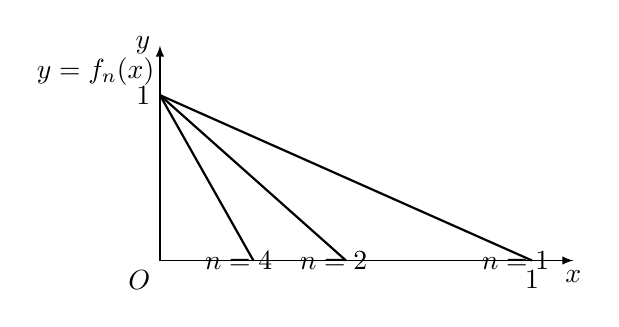
\begin{tikzpicture}[>=latex, scale=1.05]
    \draw[->] (0,0) -- (5.00,0) node[below] {$x$};
    \draw[->] (0,0) -- (0,2.60) node[left] {$y$};
    \node[below left] at (0,0) {$O$};
    \node[below] at (4.50,0) {$1$};
    \node[left] at (0,2.00) {$1$};
    % f_1: 1-x  (零点 x=1)
    \draw[thick] (0,2.00) -- (4.50,0);
    % f_2: 1-2x (零点 x=1/2)
    \draw[thick] (0,2.00) -- (2.25,0);
    % f_4: 1-4x (零点 x=1/4)
    \draw[thick] (0,2.00) -- (1.13,0);
    \node[above left] at (0.05,2.00) {$y=f_{n}(x)$};
    \node[below] at (4.30,0.22) {$n=1$};
    \node[below] at (2.10,0.22) {$n=2$};
    \node[below] at (0.95,0.22) {$n=4$};
  \end{tikzpicture}
  \caption{$f_{n}(x)=1-nx$ ($0\leqslant x\leqslant1/n$)}\label{fig:13.2.1}
\end{figure}

\begin{theorem}\label{thm:13.2.3}
如果 $[a,b]$ 上的 Riemann 可积函数列 (特别是连续函数列) $\{f_{n}(x)\}$ 在 $[a,b]$ 上一致收敛于 $f(x)$, 则 $f(x)$ 在 $[a,b]$ 上也 Riemann 可积 (连续), 且
\[
  \lim_{n\to+\infty}\int_{a}^{b}f_{n}(x)\mathrm{d}x=\int_{a}^{b}f(x)\mathrm{d}x.
\]
\end{theorem}

\begin{proof}
(参阅\extref{定理 6.3.6}) 先证 $f(x)$ 在 $[a,b]$ 上 Riemann 可积. 由于 $f_{n}(x)$ 在 $[a,b]$ 上 Riemann 可积, 根据 Lebesgue 定理 6.1.4(8), $D_{\text{不}}(f_{n})$ 为零测度集. 从定理~\ref{thm:13.2.1} 的证明或定理~\ref{thm:13.2.2}, 有
\[
  D_{\text{不}}(f(x))\subset\bigcup_{n=1}^{\infty}D_{\text{不}}(f_{n}(x)).
\]
再由\extref{引理 6.1.6}(4) 及 (2) 立即推得 $D_{\text{不}}(f(x))$ 为零测度集. 因为 $\{f_{n}(x)\}$ 在 $[a,b]$ 上一致收敛于 $f(x)$, 故 $\exists N_{0}\in\mathbb{N}$, 使得
\[
  |f(x)-f_{N_{0}}(x)|<1,\quad\forall x\in[a,b].
\]
又因 $f_{N_{0}}(x)$ 为有界函数, 不妨设 $|f_{N_{0}}(x)|\leqslant M$, $\forall x\in[a,b]$. 于是
\[
  |f(x)|\leqslant|f_{N_{0}}(x)|+1\leqslant M+1,\quad\forall x\in[a,b],
\]
即 $f(x)$ 在 $[a,b]$ 上为有界函数.

综合上述及由 Lebesgue 定理 6.1.4(8) 知 $f(x)$ 在 $[a,b]$ 上也 Riemann 可积.

另一方面, 由于 $\{f_{n}(x)\}$ 在 $[a,b]$ 上一致收敛于 $f(x)$, 故 $\forall\varepsilon>0$, $\exists N=N(\varepsilon)\in\mathbb{N}$, 当 $n>N$ 时, 有
\[
  |f_{n}(x)-f(x)|<\varepsilon,\quad\forall x\in[a,b].
\]
\[
  \begin{aligned}
    \left|\int_{a}^{b}f_{n}(x)\mathrm{d}x-\int_{a}^{b}f(x)\mathrm{d}x\right|&=\left|\int_{a}^{b}[f_{n}(x)-f(x)]\mathrm{d}x\right|\\
    &\leqslant\int_{a}^{b}|f_{n}(x)-f(x)|\mathrm{d}x<\varepsilon(b-a),
  \end{aligned}
\]
\[
  \lim_{n\to+\infty}\int_{a}^{b}f_{n}(x)\mathrm{d}x=\int_{a}^{b}f(x)\mathrm{d}x=\int_{a}^{b}\lim_{n\to+\infty}f_{n}(x)\mathrm{d}x.
\]
\end{proof}

用反证法及定理~\ref{thm:13.2.3} 立即有下面的推论.

\begin{corollary}\label{cor:13.2.3}
设 $\{f_{n}(x)\}$ 为 $[a,b]$ 上的 Riemann 可积函数, 如果
\[
  \lim_{n\to+\infty}\int_{a}^{b}f_{n}(x)\mathrm{d}x\neq\int_{a}^{b}f(x)\mathrm{d}x,
\]
则 $\{f_{n}(x)\}$ 在 $[a,b]$ 上不一致收敛.
\end{corollary}

\begin{example}[参阅例~\ref{ex:13.1.7}]\label{ex:13.2.2}
设 $\mathbb{Q}\cap[0,1]=\{r_{1},r_{2},\cdots,r_{n},\cdots\}$ 是 $[0,1]$ 上的全体有理数, 而
\[
  S_{n}(x)=\begin{cases}1, & x=r_{1},\cdots,r_{n},\\ 0, & x\text{ 为其他值},\end{cases}\qquad
  S(x)=\begin{cases}1, & x\text{ 为有理数},\\ 0, & x\text{ 为无理数}.\end{cases}
\]
显然, $\lim\limits_{n\to+\infty}S_{n}(x)=S(x)$, 且每个 $S_{n}(x)$ 在 $[0,1]$ 上是只有有限个不连续点的有界函数, 它是 Riemann 可积的. 因为 $S(x)$ 在 $[0,1]$ 上处处不连续, 所以它在 $[0,1]$ 上非 Riemann 可积.
\end{example}

现证 $\{S_{n}(x)\}$ 在 $[0,1]$ 上不一致收敛于 $S(x)$. (反证) 假设 $\{S_{n}(x)\}$ 在 $[0,1]$ 上一致收敛于 $S(x)$. 根据定理~\ref{thm:13.2.3}, $S(x)$ 在 $[0,1]$ 上必 Riemann 可积, 这与上述非 Riemann 可积相矛盾.

\begin{example}[参阅\extref{例 6.3.12}]\label{ex:13.2.3}
设 (\cref{fig:13.2.2})
\[
  f_{n}(x)=\begin{cases}
    4n^{2}x, & 0\leqslant x\leqslant\frac{1}{2n},\\
    -4n^{2}x+4n, & \frac{1}{2n}<x\leqslant\frac{1}{n},\\
    0, & \frac{1}{n}<x\leqslant1,
\end{cases}
\]
则 $f(x)=\lim\limits_{n\to+\infty}f_{n}(x)=0$. 下面证明 $\{f_{n}(x)\}$ 在 $[0,1]$ 上不一致收敛于 $f(x)=0$.
\end{example}

因为 $f(x)=0$ 连续、Riemann 可积, 故不能应用定理~\ref{thm:13.2.1} 或定理~\ref{thm:13.2.2} 或定理~\ref{thm:13.2.3} 及反证法证明 $\{f_{n}(x)\}$ 在 $[0,1]$ 上不一致收敛. 也就是不能对 $\{f_{n}(x)\}$ 在 $[0,1]$ 上是否一致收敛于 $f(x)=0$ 给出任何信息.

\begin{proof}
证法 1 (反证) 假设 $\{f_{n}(x)\}$ 在 $[0,1]$ 上一致收敛于 $f(x)=0$, 则由定理~\ref{thm:13.2.3}, 有
\[
  \begin{aligned}
    1&=\lim_{n\to+\infty}\frac{1}{2}\cdot2n\cdot\frac{1}{n}=\lim_{n\to+\infty}\int_{0}^{1}f_{n}(x)\mathrm{d}x\\
    &=\int_{0}^{1}\lim_{n\to+\infty}f_{n}(x)\mathrm{d}x=\int_{0}^{1}f(x)\mathrm{d}x=\int_{0}^{1}0\mathrm{d}x=0,
  \end{aligned}
\]
矛盾.

证法 2 (反证) 假设 $\{f_{n}(x)\}$ 在 $[0,1]$ 上一致收敛于 $f(x)=0$, 则对 $\varepsilon=\frac{1}{2}$, $\exists N\in\mathbb{N}$, 当 $n>N$ 时, 有
\[
  |f_{n}(x)-f(x)|<\varepsilon=\frac{1}{2},\quad\forall x\in[0,1].
\]
显然
\[
  2\leqslant2n=\left|4n^{2}\cdot\frac{1}{2n}-0\right|<\varepsilon=\frac{1}{2},
\]
矛盾.
\end{proof}

\begin{figure}[htbp]
  \centering
  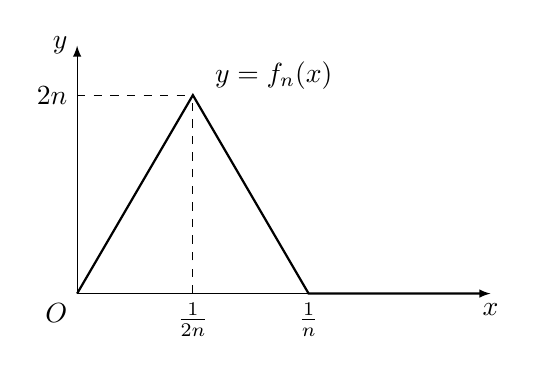
\begin{tikzpicture}[>=latex, scale=1.05]
    \draw[->] (0,0) -- (5.00,0) node[below] {$x$};
    \draw[->] (0,0) -- (0,3.00) node[left] {$y$};
    \node[below left] at (0,0) {$O$};
    \draw[thick] (0,0) -- (1.40,2.40) -- (2.80,0) -- (4.90,0);
    \draw[dashed] (1.40,0) -- (1.40,2.40);
    \draw[dashed] (0,2.40) -- (1.40,2.40);
    \node[below] at (1.40,0) {$\frac{1}{2n}$};
    \node[below] at (2.80,0) {$\frac{1}{n}$};
    \node[left] at (0,2.40) {$2n$};
    \node[above right] at (1.55,2.35) {$y=f_{n}(x)$};
  \end{tikzpicture}
  \caption{尖峰高 $2n$、底宽 $\frac{1}{n}$}\label{fig:13.2.2}
\end{figure}

\begin{example}\label{ex:13.2.4}
设 (\cref{fig:13.2.3})
\[
  f_{n}(x)=\begin{cases}
    2nx, & 0\leqslant x\leqslant\frac{1}{2n},\\
    2(1-nx), & \frac{1}{2n}<x\leqslant\frac{1}{n},\\
    0, & \frac{1}{n}<x\leqslant1,
\end{cases}
\]
则 $f(x)=\lim\limits_{n\to+\infty}f_{n}(x)=0$. 显然 $\{f_{n}(x)\}$ 在 $[0,1]$ 上一致有界 (以 $1$ 为界), 且
\[
  \begin{aligned}
    \lim_{n\to+\infty}\int_{0}^{1}f_{n}(x)\mathrm{d}x&=\lim_{n\to+\infty}\frac{1}{2}\cdot1\cdot\frac{1}{n}=0\\
    &=\int_{0}^{1}0\mathrm{d}x=\int_{0}^{1}f(x)\mathrm{d}x\\
    &=\int_{0}^{1}\lim_{n\to+\infty}f_{n}(x)\mathrm{d}x.
  \end{aligned}
\]
\end{example}

类似例~\ref{ex:13.2.3} 的理由, 因为 $f(x)=0$ 连续、Riemann 可积及
\[
  \lim_{n\to+\infty}\int_{0}^{1}f_{n}(x)\mathrm{d}x=\int_{0}^{1}\lim_{n\to+\infty}f_{n}(x)\mathrm{d}x
\]
都说明不能应用定理~\ref{thm:13.2.1} 或定理~\ref{thm:13.2.2} 或定理~\ref{thm:13.2.3} 及反证法证明 $\{f_{n}(x)\}$ 在 $[0,1]$ 上不一致收敛. 也就是不能对 $\{f_{n}(x)\}$ 在 $[0,1]$ 上是否一致收敛于 $f(x)=0$ 给出任何信息.

\begin{proof}
(反证) 假设 $\{f_{n}(x)\}$ 在 $[0,1]$ 上一致收敛于 $f(x)=0$, 则 $\varepsilon=\frac{1}{2}$, $\exists N\in\mathbb{N}$, 当 $n>N$ 时, 有
\[
  |f_{n}(x)-f(x)|<\varepsilon=\frac{1}{2},\quad\forall x\in[0,1].
\]
显然
\[
  1=|1-0|=\left|f_{n}\left(\frac{1}{2n}\right)-f\left(\frac{1}{2n}\right)\right|<\varepsilon=\frac{1}{2},
\]
矛盾.
\end{proof}

\begin{figure}[htbp]
  \centering
  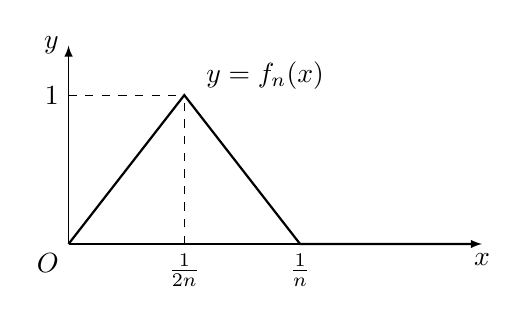
\begin{tikzpicture}[>=latex, scale=1.05]
    \draw[->] (0,0) -- (5.00,0) node[below] {$x$};
    \draw[->] (0,0) -- (0,2.40) node[left] {$y$};
    \node[below left] at (0,0) {$O$};
    \draw[thick] (0,0) -- (1.40,1.80) -- (2.80,0) -- (4.90,0);
    \draw[dashed] (1.40,0) -- (1.40,1.80);
    \draw[dashed] (0,1.80) -- (1.40,1.80);
    \node[below] at (1.40,0) {$\frac{1}{2n}$};
    \node[below] at (2.80,0) {$\frac{1}{n}$};
    \node[left] at (0,1.80) {$1$};
    \node[above right] at (1.55,1.75) {$y=f_{n}(x)$};
  \end{tikzpicture}
  \caption{尖峰高 $1$、底宽 $\frac{1}{n}$}\label{fig:13.2.3}
\end{figure}

\begin{theorem}\label{thm:13.2.4}
如果函数列 $\{f_{n}(x)\}$ 满足:

(1) 每一个 $f_{n}(x)$ 在 $[a,b]$ 上有连续的导函数;

(2) 由导函数构成的函数列 $\{f_{n}'(x)\}$ 在 $[a,b]$ 上一致收敛于函数 $g(x)$;

(3) 至少在某一点 $x_{0}\in[a,b]$ 收敛, 即 $\{f_{n}(x_{0})\}$ 收敛.

则函数列 $\{f_{n}(x)\}$ 在闭区间 $[a,b]$ 上一致收敛于某个连续可导的函数 $f(x)$, 且有
\[
  f'(x)=g(x),\quad\forall x\in[a,b],
\]
即
\[
  \lim_{n\to+\infty}f_{n}(x))'=\lim_{n\to+\infty}f_{n}'(x).
\]
\end{theorem}

\begin{proof}
因为 $\{f_{n}(x)\}$ 在 $x_{0}\in[a,b]$ 处收敛, 根据数列的 Cauchy 收敛准则, $\forall\varepsilon>0$, $\exists N_{1}\in\mathbb{N}$, 当 $n,m>N_{1}$ 时, 有
\[
  |f_{n}(x_{0})-f_{m}(x_{0})|<\frac{\varepsilon}{2}. \tag*{(1)}
\]
又因为 $\{f_{n}'(x)\}$ 在 $[a,b]$ 上一致收敛, 根据函数一致收敛的 Cauchy 收敛准则, $\exists N_{2}\in\mathbb{N}$, 当 $n,m>N_{2}$ 时, 有
\[
  |f_{n}'(x)-f_{m}'(x)|<\frac{\varepsilon}{2(b-a)},\quad\forall x\in[a,b]. \tag*{(2)}
\]
今 $N=\max\{N_{1},N_{2}\}$, 则当 $n,m>N$ 时, 不等式 (1) 与 (2) 成立.

由 Newton-Leibniz 公式, 有
\[
  f_{n}(x)=f_{n}(x_{0})+\int_{x_{0}}^{x}f_{n}'(t)\mathrm{d}t, \tag*{(3)}
\]
\[
  f_{m}(x)=f_{m}(x_{0})+\int_{x_{0}}^{x}f_{m}'(t)\mathrm{d}t,\quad\forall x\in[a,b]. \tag*{(4)}
\]
于是, 当 $n,m>N$ 时, 有
\[
  \begin{aligned}
    |f_{n}(x)-f_{m}(x)|&=\left|\left(f_{n}(x_{0})+\int_{x_{0}}^{x}f_{n}'(t)\mathrm{d}t\right)-\left(f_{m}(x_{0})+\int_{x_{0}}^{x}f_{m}'(t)\mathrm{d}t\right)\right|\\
    &=\left|f_{n}(x_{0})-f_{m}(x_{0})+\int_{x_{0}}^{x}[f_{n}'(t)-f_{m}'(t)]\mathrm{d}t\right|\\
    &\leqslant|f_{n}(x_{0})-f_{m}(x_{0})|+\left|\int_{x_{0}}^{x}|f_{n}'(t)-f_{m}'(t)|\mathrm{d}t\right|\\
    &<\frac{\varepsilon}{2}+\frac{\varepsilon}{2(b-a)}|x-x_{0}|\leqslant\varepsilon,\quad\forall x\in[a,b].
  \end{aligned}
\]
根据函数列一致收敛的 Cauchy 收敛准则, $\{f_{n}(x)\}$ 在 $[a,b]$ 上一致收敛. 设其极限函数为 $f(x)$.

由于 $\{f_{n}'(x)\}$ 在 $[a,b]$ 上一致收敛于 $g(x)$, $f_{n}'(x)$ 连续 ($\forall n\in\mathbb{N}$), 从定理~\ref{thm:13.2.1} 推得 $g(x)$ 在 $[a,b]$ 连续.

\[
  \lim_{n\to+\infty}\int_{x_{0}}^{x}f_{n}'(t)\mathrm{d}t\xlongequal{\text{定理~\ref{thm:13.2.3}}}\int_{x_{0}}^{x}\lim_{n\to+\infty}f_{n}'(t)\mathrm{d}t=\int_{x_{0}}^{x}g(t)\mathrm{d}t.
\]
在 (3) 式两边取 $n\to+\infty$ 得到
\[
  \lim_{n\to+\infty}f_{n}(x)=\lim_{n\to+\infty}\left[f_{n}(x_{0})+\int_{x_{0}}^{x}f_{n}'(t)\mathrm{d}t\right],
\]
即
\[
  f(x)=f(x_{0})+\int_{x_{0}}^{x}g(t)\mathrm{d}t.
\]
应用微积分的基本定理 6.3.2 即得
\[
  \lim_{n\to+\infty}f_{n}(x))'=f'(x)=g(x)=\lim_{n\to+\infty}f_{n}'(x).
\]
\end{proof}

用反证法及定理~\ref{thm:13.2.4} 立即有下面的推论.

\begin{corollary}\label{cor:13.2.4}
如果函数列 $\{f_{n}(x)\}$ 满足定理~\ref{thm:13.2.4} 中的 (1) 与 (3), 且
\[
  \lim_{n\to+\infty}f_{n}(x))'\neq\lim_{n\to+\infty}f_{n}'(x),
\]
则 $\{f_{n}'(x)\}$ 在 $[a,b]$ 上不一致收敛.
\end{corollary}

现在我们来考察定理~\ref{thm:13.2.1} 的逆定理是否成立, 即如果连续函数列 $\{f_{n}(x)\}$ 在 $[a,b]$ 上收敛于连续函数 $f(x)$, 问: $\{f_{n}(x)\}$ 在 $[a,b]$ 上是否一致收敛于 $f(x)$? 一般说来, 答案是否定的. 例~\ref{ex:13.2.3} 与例~\ref{ex:13.2.4} 都是反例. 如果附加条件: $\forall x\in[a,b]$, 数列 $\{f_{n}(x)\}$ 单调减收敛于 $0$, 则 $\{f_{n}(x)\}$ 在 $[a,b]$ 上一致收敛于 $f(x)$.

\begin{theorem}[Dini]\label{thm:13.2.5}
设函数列 $\{f_{n}(x)\}$ 在有界闭区间 $[a,b]$ 上连续, 如果 $\forall x\in[a,b]$, 数列 $\{f_{n}(x)\}$ 单调减收敛于 $0$, 则 $\{f_{n}(x)\}$ 在 $[a,b]$ 上一致收敛于 $f(x)=0$.
\end{theorem}

\begin{proof}
证法 1 $\forall\varepsilon>0$, $\exists N_{x}=N(x,\varepsilon)\in\mathbb{N}$, 使得
\[
  0\leqslant f_{N_{x}}(x)<\varepsilon.
\]
由于 $f_{N_{x}}(x)$ 在点 $x$ 连续, 必 $\exists\delta_{x}>0$, 使得当 $t\in[a,b]$ 且 $t\in(x-\delta_{x},x+\delta_{x})$ 时仍有
\[
  0\leqslant f_{N_{x}}(t)<\varepsilon.
\]
于是, 这些开区间 $\{(x-\delta_{x},x+\delta_{x})\mid x\in[a,b]\}$ 构成了 $[a,b]$ 的一个开覆盖. 根据 Heine-Borel 有限覆盖定理, 存在有限子覆盖 $\{(x_{i}-\delta_{x_{i}},x_{i}+\delta_{x_{i}})\mid i=1,2,\cdots,m\}$. 令 $N=\max\{N_{x_{1}},N_{x_{2}},\cdots,N_{x_{m}}\}$, 则当 $n>N$ 时, $\forall x\in[a,b]$, 必有 $x\in(x_{i}-\delta_{x_{i}},x_{i}+\delta_{x_{i}})$, 从而
\[
  0\leqslant f_{n}(x)\leqslant f_{N}(x)\leqslant f_{N_{x}}(x)<\varepsilon.
\]
这就证明了 $f_{n}(x)\rightrightarrows0=f(x)$, $x\in[a,b]$, $n\to+\infty$.

证法 2 (反证) 假设 $\{f_{n}(x)\}$ 在 $[a,b]$ 上不一致收敛于 $0$, 则 $\exists\varepsilon_{0}>0$, 使得 $\forall n\in\mathbb{N}$, 必有 $k_{n}>n$ 及 $x_{n}$ 满足 $f_{k_{n}}(x_{n})\geqslant\varepsilon_{0}$. 因为 $x_{n}\in[a,b]$, 根据 Bolzano-Weierstrass 的序列紧性定理, $\{x_{n}\}$ 有子列收敛于 $x_{0}\in[a,b]$, 这个子列仍记为 $\{x_{n}\}$. 此外, 可选 $k_{1}<k_{2}<\cdots<k_{n}<k_{n+1}<\cdots$. 由于 $\forall x\in[a,b]$, $\{f_{n}(x)\}$ 单调减少, 故当 $m>n$ 时, 有
\[
  f_{k_{n}}(x_{m})\geqslant f_{k_{m}}(x_{m})\geqslant\varepsilon_{0}.
\]
再从 $f_{n}(x)$ 连续推得
\[
  f_{k_{n}}(x_{0})=\lim_{n\to+\infty}f_{k_{n}}(x_{m})\geqslant\varepsilon_{0},
\]
\[
  0=\lim_{n\to+\infty}f_{k_{n}}(x_{0})\geqslant\varepsilon_{0}>0,
\]
矛盾.
\end{proof}

%  第二部分：定理 13.2.1' 起（生成脚本 tools/_make_ch13_2b.py）
% ==================================================================

%  第二部分：定理 13.2.1' 起（生成脚本 tools/_make_ch13_2b.py）
% ==================================================================

% ===== PART-B =====

设 $S_{n}(x)=\sum_{k=1}^{n}u_{k}(x)$, $S(x)=\sum_{n=1}^{\infty}u_{n}(x)$, 考虑到函数项级数 $\sum_{n=1}^{\infty}u_{n}(x)$ 与 $\{S_{n}(x)\}$ 之间的关系. 对于函数项级数有相应的结果. 自然可以不必重新证明, 对偶地叙述即可. 但是, 为了让读者都用函数项级数论述得到锻炼, 我们还是阐述一遍.

\setcounter{theorem}{1}
\begin{theoremp}\label{thm:13.2.1p}
如果函数项级数 $\sum_{n=1}^{\infty}u_{n}(x)$ 在 $I\subseteq\mathbb{R}$ 上一致收敛于 $S(x)$, 且每个 $u_{n}(x)$ 都在 $I$ 上连续, 则和函数 $S(x)=\sum_{n=1}^{\infty}u_{n}(x)$ 在 $I$ 上也连续.
\end{theoremp}

\begin{proof}
证法 1 应用定理~\ref{thm:13.2.1}.

证法 2 $\forall x_{0}\in I$, 由于 $\sum_{n=1}^{\infty}u_{n}(x)$ 在 $I$ 上一致收敛于 $S(x)$, 故 $\forall\varepsilon>0$, $\exists N=N(\varepsilon)\in\mathbb{N}$, 当 $n>N$ 时, 有
\[
  \Big|\sum_{k=n+1}^{\infty}u_{k}(x)\Big|=\Big|\sum_{k=1}^{n}u_{k}(x)-\sum_{k=1}^{\infty}u_{k}(x)\Big|<\varepsilon,\quad\forall x\in I.
\]
由于 $S_{N+1}(x)=\sum_{k=1}^{N+1}u_{k}(x)$ 在 $x_{0}$ 连续, 故 $\exists\delta>0$, 当 $|x-x_{0}|<\delta$ 时, 有
\[
  \left|\sum_{k=1}^{N+1}u_{k}(x)-\sum_{k=1}^{N+1}u_{k}(x_{0})\right|<\frac{\varepsilon}{3}.
\]
于是
\[
  \begin{aligned}
    \left|\sum_{k=1}^{\infty}u_{k}(x)-\sum_{k=1}^{\infty}u_{k}(x_{0})\right|&\leqslant\left|\sum_{k=N+2}^{\infty}u_{k}(x)\right|+\left|\sum_{k=1}^{N+1}u_{k}(x)-\sum_{k=1}^{N+1}u_{k}(x_{0})\right|+\left|\sum_{k=N+2}^{\infty}u_{k}(x_{0})\right|\\
    &<\frac{\varepsilon}{3}+\frac{\varepsilon}{3}+\frac{\varepsilon}{3}=\varepsilon,
  \end{aligned}
\]
即 $S(x)=\sum_{n=1}^{\infty}u_{n}(x)$ 在 $x_{0}$ 处连续. 由 $x_{0}\in I$ 的任取性, $S(x)=\sum_{n=1}^{\infty}u_{n}(x)$ 在 $I$ 上连续.
\end{proof}

\setcounter{corollary}{1}
\begin{corollaryp}\label{cor:13.2.1p}
如果函数项级数 $\sum_{n=1}^{\infty}u_{n}(x)$ 在 $I\subset\mathbb{R}$ 上收敛于和函数 $S(x)$. 又 $u_{n}(x)$ 在 $I$ 上连续 ($n\in\mathbb{N}$), 且 $S(x)$ 在 $I$ 上不连续, 则 $\sum_{n=1}^{\infty}u_{n}(x)$ 在 $I$ 上不一致收敛.
\end{corollaryp}

\begin{proof}
证法 1 应用推论~\ref{cor:13.2.1}.

证法 2 (反证) 假设 $\sum_{n=1}^{\infty}u_{n}(x)$ 在 $I$ 上一致收敛, 根据定理~\ref{thm:13.2.1p}, 和函数 $S(x)=\sum_{n=1}^{\infty}u_{n}(x)$ 在 $I$ 上为连续函数, 这与已知 $S(x)$ 在 $I$ 上不连续相矛盾.
\end{proof}

应用推论~\ref{cor:13.2.1p} 得到例~\ref{ex:13.1.1} 中的 $x^{1}+\sum_{n=2}^{\infty}(x^{n}-x^{n-1})$ 在 $(-1,1]$ 上不一致收敛;

例~\ref{ex:13.1.6} 中的 $\sum_{n=1}^{\infty}[\mathrm{e}^{-n^{2}x^{2}}-\mathrm{e}^{-(n-1)^{2}x^{2}}]$ 在 $[0,1]$ 上不一致收敛.

更一般地, 有下面的定理.

\setcounter{theorem}{2}
\begin{theoremp}[逐项求极限 —— 和号与极限号可交换]\label{thm:13.2.2p}
设 $u_{n}(x)$ 在集合 $I\subset\mathbb{R}$ 有定义, 如果 $\lim\limits_{x\to a}u_{n}(x)=c_{n}$, $\forall n\in\mathbb{N}$. 又函数项级数 $\sum_{n=1}^{\infty}u_{n}(x)$ 在 $I$ 上一致收敛, 则 $\sum_{n=1}^{\infty}c_{n}$ 收敛, 且
\[
  \lim_{x\to a}\sum_{n=1}^{\infty}u_{n}(x)=\sum_{n=1}^{\infty}c_{n}=\sum_{n=1}^{\infty}\lim_{x\to a}u_{n}(x),
\]
其中 $a$ 可为 $a^{+}$, $a^{-}$, $+\infty$, $-\infty$, $\infty$.
\end{theoremp}

\begin{proof}
证法 1 应用定理~\ref{thm:13.2.2}.

证法 2 先证 $\sum_{n=1}^{\infty}c_{n}$ 收敛.

由于 $\sum_{n=1}^{\infty}u_{n}(x)$ 在 $I$ 上一致收敛, 故 $\forall\varepsilon>0$, 根据函数项级数一致收敛的 Cauchy 收敛准则, $\exists N\in\mathbb{N}$, 当 $n>N$ 时, 有
\[
  \left|\sum_{k=n+1}^{n+p}u_{k}(x)\right|<\frac{\varepsilon}{6},\quad\forall p\in\mathbb{N};
\]
令 $p\to+\infty$ 得到 $\left|\sum_{k=n+1}^{\infty}u_{k}(x)\right|\leqslant\frac{\varepsilon}{6}$. 由 $x\to a$ 得到
\[
  \Big|\sum_{k=n+1}^{n+p}c_{k}\Big|\leqslant\frac{\varepsilon}{6}.
\]
再由数项级数的 Cauchy 收敛原理, 级数 $\sum_{n=1}^{\infty}c_{n}$ 收敛.

对上述的 $\varepsilon>0$ 及 $N\in\mathbb{N}$, $n>N$, 有
\[
  \Big|\sum_{k=1}^{n}c_{k}-\sum_{k=1}^{\infty}c_{k}\Big|=\Big|\sum_{k=n+1}^{\infty}c_{k}\Big|=\lim_{p\to+\infty}\Big|\sum_{k=n+1}^{n+p}c_{k}\Big|\leqslant\frac{\varepsilon}{6}.
\]
设 $a\in\mathbb{R}$, 因为 $\lim\limits_{x\to a}u_{n}(x)=c_{n}$, 故 $\exists\delta>0$, 当 $0<|x-a|<\delta$ 时, 有
\[
  \left|\sum_{k=1}^{N+1}u_{k}(x)-\sum_{k=1}^{N+1}c_{k}\right|<\frac{\varepsilon}{3}.
\]
于是, 当 $0<|x-a|<\delta$ 时, 有
\[
  \begin{aligned}
    \left|\sum_{n=1}^{\infty}u_{n}(x)-\sum_{n=1}^{\infty}c_{n}\right|&\leqslant\left|\sum_{n=1}^{\infty}u_{n}(x)-\sum_{n=1}^{N+1}u_{n}(x)\right|\\
    &\quad+\left|\sum_{n=1}^{N+1}u_{n}(x)-\sum_{n=1}^{N+1}c_{n}\right|+\left|\sum_{n=1}^{N+1}c_{n}-\sum_{n=1}^{\infty}c_{n}\right|\\
    &=\left|\sum_{n=N+2}^{\infty}u_{n}(x)\right|+\left|\sum_{k=1}^{N+1}u_{n}(x)-\sum_{n=1}^{N+1}c_{n}\right|+\left|\sum_{n=N+2}^{\infty}c_{n}\right|\\
    &<\frac{\varepsilon}{6}+\frac{\varepsilon}{3}+\frac{\varepsilon}{6}<\varepsilon.
  \end{aligned}
\]
这就证明了 $\lim\limits_{x\to a}\sum_{n=1}^{\infty}u_{n}(x)=\sum_{n=1}^{\infty}c_{n}=\sum_{n=1}^{\infty}\lim\limits_{x\to a}u_{n}(x)$.
\end{proof}

用反证法及定理~\ref{thm:13.2.2} 立即有下面的推论.

\setcounter{corollary}{2}
\begin{corollaryp}\label{cor:13.2.2p}
设 $u_{n}(x)$ 在集合 $I\subset\mathbb{R}$ 上有定义, 且 $\lim\limits_{x\to a}u_{n}(x)=c_{n}$, $\forall n\in\mathbb{N}$. 如果 $\sum_{n=1}^{\infty}c_{n}$ 不收敛, 或即使 $\sum_{n=1}^{\infty}c_{n}$ 收敛但
\[
  \lim_{x\to a}\sum_{n=1}^{\infty}u_{n}(x)\neq\sum_{n=1}^{\infty}c_{n}=\sum_{n=1}^{\infty}\lim_{x\to a}u_{n}(x),
\]
则 $\sum_{n=1}^{\infty}u_{n}(x)$ 在 $I$ 上不一致收敛.
\end{corollaryp}

\setcounter{theorem}{3}
\begin{theoremp}[逐项积分 —— 积分号与和号可交换]\label{thm:13.2.3p}
如果函数项级数 $\sum_{n=1}^{\infty}u_{n}(x)$ 在闭区间 $I=[a,b]$ 上一致收敛于 $S(x)$, $\forall n\in\mathbb{N}$, $u_{n}(x)$ 在 $[a,b]$ 上 Riemann 可积 (连续), 则 $S(x)=\sum_{n=1}^{\infty}u_{n}(x)$ 在 $[a,b]$ 上也 Riemann 可积 (连续), 且
\[
  \begin{aligned}
    \int_{a}^{b}S(x)\mathrm{d}x&=\int_{a}^{b}\lim_{n\to+\infty}S_{n}(x)\mathrm{d}x=\int_{a}^{b}\sum_{n=1}^{\infty}u_{n}(x)\mathrm{d}x\\
    &=\sum_{n=1}^{\infty}\int_{a}^{b}u_{n}(x)\mathrm{d}x=\lim_{n\to+\infty}\int_{a}^{b}S_{n}(x)\mathrm{d}x.
  \end{aligned}
\]
\end{theoremp}

\begin{proof}
证法 1 应用定理~\ref{thm:13.2.3}.

证法 2 先证 $S(x)=\sum_{n=1}^{\infty}u_{n}(x)$ 在 $[a,b]$ 上 Riemann 可积. 由于 $u_{n}(x)$ 在 $[a,b]$ 上 Riemann 可积, 根据 Lebesgue 定理 6.1.4(8), $D_{\text{不}}(u_{n})$ 为零测集. 从定理~\ref{thm:13.2.1p} 或定理~\ref{thm:13.2.2p}, $D_{\text{不}}(S)\subset\bigcup_{n=1}^{\infty}D_{\text{不}}(u_{n})$. 再由\extref{引理 6.1.6}(4) 及 (2) 立即推得 $D_{\text{不}}(S)$ 为零测集.

因为 $\sum_{n=1}^{\infty}u_{n}(x)$ 在 $[a,b]$ 上一致收敛于 $S(x)$, 故 $\exists N_{0}\in\mathbb{N}$, 使得
\[
  \left|S(x)-\sum_{k=1}^{N_{0}}u_{k}(x)\right|<1,\quad\forall x\in[a,b].
\]
因为 $\sum_{k=1}^{N_{0}}u_{k}(x)$ 在 $[a,b]$ 上 Riemann 可积, 故有界. 设 $\left|\sum_{k=1}^{N_{0}}u_{k}(x)\right|\leqslant M$, $\forall x\in[a,b]$. 于是
\[
  \left|\sum_{n=1}^{\infty}u_{n}(x)\right|=|S(x)|\leqslant\left|\sum_{k=1}^{N_{0}}u_{k}(x)\right|+1\leqslant M+1.
\]
这就证明了 $S(x)=\sum_{n=1}^{\infty}u_{n}(x)$ 在 $[a,b]$ 为有界函数. 综合上述及由 Lebesgue 定理 6.1.4(8) 知, $S(x)=\sum_{n=1}^{\infty}u_{n}(x)$ 在 $[a,b]$ 上 Riemann 可积.

从 $\sum_{n=1}^{\infty}u_{n}(x)$ 在 $[a,b]$ 上一致收敛知, $\forall\varepsilon>0$, $\exists N=N(\varepsilon)\in\mathbb{N}$, 当 $n>N$, 有
\[
  \left|\sum_{k=1}^{n}u_{k}(x)-\sum_{k=1}^{\infty}u_{k}(x)\right|=\left|\sum_{k=n+1}^{\infty}u_{k}(x)\right|<\frac{\varepsilon}{b-a},\quad\forall x\in[a,b].
\]
于是, 当 $n>N$ 时, 有
\[
  \left|\sum_{k=1}^{n}\int_{a}^{b}u_{k}(x)\mathrm{d}x-\int_{a}^{b}\sum_{k=1}^{\infty}u_{k}(x)\mathrm{d}x\right|=\left|\int_{a}^{b}\sum_{k=n+1}^{\infty}u_{k}(x)\mathrm{d}x\right|
\]
\[
  \leqslant\int_{a}^{b}\left|\sum_{k=n+1}^{\infty}u_{k}(x)\right|\mathrm{d}x<\frac{\varepsilon}{b-a}\cdot(b-a)=\varepsilon,
\]
所以
\[
  \sum_{k=1}^{\infty}\int_{a}^{b}u_{k}(x)\mathrm{d}x=\lim_{n\to+\infty}\sum_{k=1}^{n}\int_{a}^{b}u_{k}(x)\mathrm{d}x=\int_{a}^{b}\sum_{k=1}^{\infty}u_{k}(x)\mathrm{d}x.
\]
\end{proof}

用反证法及定理~\ref{thm:13.2.3} 立即有下面的推论.

\setcounter{corollary}{3}
\begin{corollaryp}\label{cor:13.2.3p}
设 $u_{n}(x)$ 在 $[a,b]$ 上 Riemann 可积, 如果 $S(x)=\sum_{n=1}^{\infty}u_{n}(x)$ 在 $[a,b]$ 上非 Riemann 可积, 或即使 Riemann 可积, 如果
\[
  \int_{a}^{b}\sum_{n=1}^{\infty}u_{n}(x)\mathrm{d}x\neq\sum_{n=1}^{\infty}\int_{a}^{b}u_{n}(x)\mathrm{d}x,
\]
则 $\sum_{n=1}^{\infty}u_{n}(x)$ 在 $[a,b]$ 上不一致收敛.
\end{corollaryp}

\begin{example}[参阅例~\ref{ex:13.1.5}]\label{ex:13.2.5}
设 $u_{n}(x)=nx(1-x^{2})^{n}-(n-1)x(1-x^{2})^{n-1}$, $n=1,2,\cdots$. 证明: $\sum_{n=1}^{\infty}u_{n}(x)$ 在 $[0,1]$ 不一致收敛.
\end{example}

\begin{proof}
证法 1 从例~\ref{ex:13.1.5} 得到
\[
  \int_{0}^{1}\sum_{n=1}^{\infty}u_{n}(x)\mathrm{d}x\neq\sum_{n=1}^{\infty}\int_{0}^{1}u_{n}(x)\mathrm{d}x.
\]
根据推论~\ref{cor:13.2.3p} 知, $\sum_{n=1}^{\infty}u_{n}(x)$ 在 $[0,1]$ 上不一致收敛.

证法 2 因为
\[
  \begin{aligned}
    \beta_{n}&=\sup_{x\in[0,1]}|S_{n}(x)-S(x)|=\sup_{x\in[0,1]}nx(1-x^{2})^{n}\\
    &\geqslant n\cdot\frac{1}{n}\left(1-\frac{1}{n^{2}}\right)^{n}=\left(1-\frac{1}{n}\right)^{n}\left(1+\frac{1}{n}\right)^{n}\to\mathrm{e}^{-1}\cdot\mathrm{e}=1\quad(n\to+\infty).
  \end{aligned}
\]
所以, $\lim\limits_{n\to+\infty}\beta_{n}\neq0$, 从而 $\sum_{n=1}^{\infty}u_{n}(x)$ 在 $[0,1]$ 上不一致收敛.
\end{proof}

\setcounter{theorem}{4}
\begin{theoremp}[逐项求导 —— 求导与和号可交换]\label{thm:13.2.4p}
如果 $\sum_{n=1}^{\infty}u_{n}(x)$ 满足:

(1) $u_{n}(x)$ 在 $[a,b]$ 上连续可导, $n\in\mathbb{N}$;

(2) $\sum_{n=1}^{\infty}u_{n}'(x)$ 在 $[a,b]$ 上一致收敛 (于 $g(x)$);

(3) 至少在某一点 $x_{0}\in[a,b]$, $\sum_{n=1}^{\infty}u_{n}(x_{0})$ 收敛.

则 $S(x)=\sum_{n=1}^{\infty}u_{n}(x)$ 在 $[a,b]$ 上连续可导, 且
\[
  S'(x)=\left(\sum_{n=1}^{\infty}u_{n}(x)\right)'=\sum_{n=1}^{\infty}u_{n}'(x).
\]
\end{theoremp}

\begin{proof}
证法 1 应用定理~\ref{thm:13.2.4}.

证法 2 由条件 (2)、条件 (3) 及定理~\ref{thm:13.2.1} 知, $\sum_{n=1}^{\infty}u_{n}'(x)$ 在 $[a,b]$ 上连续, 从而在 $[a,b]$ 上 Riemann 可积. 令 $\sigma(x)=\sum_{n=1}^{\infty}u_{n}'(x)$, $\forall x\in[a,b]$. 根据条件 (2) 及定理~\ref{thm:13.2.3p} 得到
\[
  \begin{aligned}
    \int_{x_{0}}^{x}\sigma(t)\mathrm{d}t&=\int_{x_{0}}^{x}\left(\sum_{n=1}^{\infty}u_{n}'(t)\right)\mathrm{d}t\xlongequal{\text{条件 (2)}}\sum_{n=1}^{\infty}\int_{x_{0}}^{x}u_{n}'(t)\mathrm{d}t\\
    &\xlongequal{\text{Newton-Leibniz}}\sum_{n=1}^{\infty}[u_{n}(x)-u_{n}(x_{0})]\xlongequal{\text{条件 (3)}}S(x)-S(x_{0}).
  \end{aligned}
\]
再由 $\sigma(x)$ 连续, 有
\[
  \begin{aligned}
    \sum_{n=1}^{\infty}u_{n}'(x)&=\sigma(x)\xlongequal{\text{微积分基本定理}}\left(\int_{x_{0}}^{x}\sigma(t)\mathrm{d}t\right)'\\
    &=[S(x)-S(x_{0})]'=S'(x)=\left(\sum_{n=1}^{\infty}u_{n}(x)\right)'.
  \end{aligned}
\]
\end{proof}

用反证法及定理~\ref{thm:13.2.4} 立即有下面的推论.

\setcounter{corollary}{4}
\begin{corollaryp}\label{cor:13.2.4p}
如果 $\sum_{n=1}^{\infty}u_{n}(x)$ 满足定理~\ref{thm:13.2.4p} 中的条件 (1) 与条件 (3), 且
\[
  \Big(\sum_{n=1}^{\infty}u_{n}(x)\Big)'\neq\sum_{n=1}^{\infty}u_{n}'(x),
\]
则 $\sum_{n=1}^{\infty}u_{n}'(x)$ 在 $[a,b]$ 上不一致收敛.
\end{corollaryp}

\setcounter{theorem}{5}
\begin{theoremp}[Dini]\label{thm:13.2.5p}
设函数项级数 $\sum_{n=1}^{\infty}u_{n}(x)$ 的每一项 $u_{n}(x)$ 在有界闭区间 $[a,b]$ 上连续且非负, 且和函数 $\sum_{n=1}^{\infty}u_{n}(x)$ 也在 $[a,b]$ 上连续, 则 $\sum_{n=1}^{\infty}u_{n}(x)$ 在 $[a,b]$ 上一致收敛.
\end{theoremp}

\begin{proof}
因为 $u_{n}(x)$ 在 $[a,b]$ 上连续非负, 则 $S_{n}(x)=\sum_{k=1}^{n}u_{k}(x)$ 也在 $[a,b]$ 上连续. 令 $f_{n}(x)=S(x)-S_{n}(x)=\sum_{k=1}^{\infty}u_{k}(x)-\sum_{k=1}^{n}u_{k}(x)=\sum_{k=n+1}^{\infty}u_{k}(x)$, 于是 $\{f_{n}(x)\}$ 在 $[a,b]$ 上连续且单调减收敛于 $0$. 根据 Dini 定理~\ref{thm:13.2.5} 推得, $\{f_{n}(x)\}$ 在 $[a,b]$ 上一致收敛于 $0$, 从而 $\{S_{n}(x)\}=\{S(x)-f_{n}(x)\}$ 在 $[a,b]$ 上一致收敛于 $S(x)-0=S(x)$.
\end{proof}

注意, 如果将 Dini 定理~\ref{thm:13.2.5p} 中的有界闭区间 $[a,b]$ 换成开区间或无穷区间, 结论就可能不成立.

\begin{example}\label{ex:13.2.6}
函数项级数 $\sum_{n=0}^{\infty}x^{n}$ 的每一项 $x^{n}$ 在 $[0,1)$ 上非负连续, 它的和函数 $S(x)=\frac{1}{1-x}$ 也在 $[0,1)$ 上连续, 但该函数项级数 $\sum_{n=1}^{\infty}x^{n}$ 在 $[0,1)$ 上不一致收敛.
\end{example}

\begin{proof}
证法 1 因为
\[
  \beta_{n}=\sup_{x\in[0,1)}|x^{n}-0|=1\not\to0\quad(n\to+\infty),
\]
所以 $x^{n}\not\rightrightarrows0$, $x\in[0,1)$, $n\to+\infty$. 根据推论~\ref{cor:13.1.1} 立刻 $\sum_{n=0}^{\infty}x^{n}$ 在 $[0,1)$ 上不一致收敛.

证法 2 (反证) 假设 $\sum_{n=0}^{\infty}x^{n}$ 在 $[0,1)$ 上一致收敛, 则由定理~\ref{thm:13.2.2p} 知
\[
  \lim_{x\to1^{-}}\sum_{n=0}^{\infty}x^{n}=\sum_{n=0}^{\infty}\lim_{x\to1^{-}}x^{n}=\sum_{n=0}^{\infty}1
\]
收敛, 这与 $\sum_{n=0}^{\infty}1=+\infty$ 显然发散相矛盾.
\end{proof}

\begin{example}\label{ex:13.2.7}
证明: 函数项级数 $\sum_{n=1}^{\infty}\frac{n+x}{n^{3}}$

(1) 为 $[0,+\infty)$ 上的连续函数;

(2) 在 $[0,+\infty)$ 上不一致收敛.
\end{example}

\begin{proof}
(1) $\forall x_{0}\in[0,+\infty)$, $\exists M>0$, 使得 $x\in[0,M)$, 则
\[
  \left|\frac{n+x}{n^{3}}\right|\leqslant\frac{n+M}{n^{3}}.
\]
由于
\[
  \sum_{n=1}^{\infty}\frac{n+M}{n^{3}}=\sum_{n=1}^{\infty}\left(\frac{1}{n^{2}}+\frac{M}{n^{3}}\right)
\]
收敛, 根据 Weierstrass 判别法推得函数项级数 $\sum_{n=1}^{\infty}\frac{n+x}{n^{3}}$ 在 $[0,M)$ 上一致收敛, 根据定理~\ref{thm:13.2.1p}, $\sum_{n=1}^{\infty}\frac{n+x}{n^{3}}$ 在 $[0,M)$ 上连续, 当然在 $x_{0}\in[0,M)$ 连续. 因为 $x_{0}$ 是任取的, 所以 $\sum_{n=1}^{\infty}\frac{n+x}{n^{3}}$ 为 $[0,+\infty)$ 上的连续函数.

(2) 因为
\[
  \beta_{n}=\sup_{x\in[0,+\infty)}\left|\frac{n+x}{n^{3}}-0\right|\geqslant\frac{n+n^{3}}{n^{3}}=1+\frac{1}{n^{2}}\geqslant1,
\]
或
\[
  \beta_{n}=\sup_{x\in[0,+\infty)}\left|\frac{n+x}{n^{3}}-0\right|=\sup_{x\in[0,+\infty)}\frac{n+x}{n^{3}}=+\infty,
\]
所以, $\lim\limits_{n\to+\infty}\beta_{n}\neq0$. 根据定理~\ref{thm:13.1.2}, $\frac{n+x}{n^{3}}\not\rightrightarrows0$, $x\in[0,+\infty)$, $n\to+\infty$. 再由推论~\ref{cor:13.1.1}, $\sum_{n=1}^{\infty}\frac{n+x}{n^{3}}$ 在 $[0,+\infty)$ 上不一致收敛.
\end{proof}

\begin{example}\label{ex:13.2.8}
设 $S(x)=\sum_{n=0}^{\infty}\frac{x^{n}}{3^{n}}\cos n\pi x^{2}$, 计算 $\lim\limits_{x\to1}S(x)$.
\end{example}

\begin{proof}
在含 $1$ 的区间 $[-2,2]$ 上考察这个函数项级数. 由于
\[
  \left|\frac{x^{n}}{3^{n}}\cos n\pi x^{2}\right|\leqslant\left(\frac{2}{3}\right)^{n}
\]
及 $\sum_{n=1}^{\infty}\left(\frac{2}{3}\right)^{n}$ 收敛, 根据 Weierstrass 判别法知原级数在 $[-2,2]$ 上一致收敛, $S(x)$ 是 $[-2,2]$ 上的连续函数. 于是
\[
  \lim_{x\to1}S(x)=S(1)=\sum_{n=0}^{\infty}\frac{\cos n\pi}{3^{n}}=\sum_{n=0}^{\infty}\frac{(-1)^{n}}{3^{n}}=\sum_{n=0}^{\infty}\left(-\frac{1}{3}\right)^{n}=\frac{1}{1-\left(-\frac{1}{3}\right)}=\frac{3}{4}.
\]
\end{proof}

\begin{example}\label{ex:13.2.9}
证明: $S(x)=\sum_{n=1}^{\infty}n\mathrm{e}^{-nx}$ 在 $(0,+\infty)$ 上连续. 进而, $S(x)$ 为 $C^{\infty}$ 函数.
\end{example}

\begin{proof}
例~\ref{ex:13.1.13}(2) 已经证明了这函数项级数在 $(0,+\infty)$ 上不一致收敛, 因而不能直接用定理~\ref{thm:13.2.1p} 来证明 $S(x)$ 为 $(0,+\infty)$ 上的连续函数.

仿例~\ref{ex:13.2.7}(1) 的证明, 考虑 $\forall x_{0}\in(0,+\infty)$, 取 $\delta$, 使得 $0<\delta<x_{0}$, 由例~\ref{ex:13.1.13}(1) 知 $\sum_{n=1}^{\infty}n\mathrm{e}^{-nx}$ 在 $[\delta,+\infty)$ 上一致收敛. 根据定理~\ref{thm:13.2.1p}, $S(x)$ 在 $[\delta,+\infty)$ 中为连续函数, 因而 $S(x)$ 在 $x_{0}$ 点处连续. 由于 $x_{0}$ 是 $(0,+\infty)$ 中的任一点, 所以 $S(x)$ 为 $(0,+\infty)$ 上的连续函数.

进而, 从 $\left|(-1)^{k}n^{k+1}\mathrm{e}^{-nx}\right|=\frac{n^{k+1}}{\mathrm{e}^{nx}}\leqslant\frac{n^{k+1}}{\mathrm{e}^{n\delta}}$, $\forall x\in[\delta,+\infty)$, $\delta>0$ 及
\[
  \sqrt[n]{\frac{n^{k+1}}{\mathrm{e}^{n\delta}}}=\frac{(\sqrt[n]{n})^{k+1}}{\mathrm{e}^{\delta}}\to\frac{1}{\mathrm{e}^{\delta}}<1\quad(n\to+\infty),
\]
并根据 Cauchy 判别法的极限形式, $\sum_{n=1}^{\infty}\frac{n^{k+1}}{\mathrm{e}^{n\delta}}$ 收敛.

或者由
\[
  \frac{(n+1)^{k+1}}{\mathrm{e}^{(n+1)\delta}}\bigg/\frac{n^{k+1}}{\mathrm{e}^{n\delta}}=\left(1+\frac{1}{n}\right)^{k+1}\bigg/\mathrm{e}^{\delta}\to\frac{1}{\mathrm{e}^{\delta}}<1\quad(n\to+\infty),
\]
根据 $d'$Alembert 判别法的极限形式, $\sum_{n=1}^{\infty}\frac{n^{k+1}}{\mathrm{e}^{n\delta}}$ 收敛.

再由 Weierstrass 判别法知
\[
  \sum_{n=1}^{\infty}(-1)^{k}n^{k+1}\mathrm{e}^{-nx}
\]
在 $[\delta,+\infty)$ 上一致收敛.

类似连续性的证明, $\forall x_{0}\in(0,+\infty)$ 取 $\delta$, 使得 $0<\delta<x_{0}$, 则函数项级数 $\sum_{n=1}^{\infty}(-1)^{k}n^{k+1}\mathrm{e}^{-nx}$ 在 $[\delta,+\infty)$ 中一致收敛. 应用定理~\ref{thm:13.2.4p}, 得
\[
  \begin{aligned}
    S^{(k)}(x)&=-(S^{(k-1)}(x))'=\left(\sum_{n=1}^{\infty}(-1)^{k-1}n^{k}\mathrm{e}^{-nx}\right)'\\
    &=\sum_{n=1}^{\infty}[(-1)^{k-1}n^{k}\mathrm{e}^{-nx}]'=\sum_{n=1}^{\infty}(-1)^{k}n^{k+1}\mathrm{e}^{-nx},\quad k=1,2,\cdots.
  \end{aligned}
\]
所以, $S(x)=\sum_{n=1}^{\infty}n\mathrm{e}^{-nx}$ 为 $C^{\infty}$ 函数.
\end{proof}

\begin{example}\label{ex:13.2.10}
设 $S(x)=\sum_{n=1}^{\infty}\frac{\cos nx}{n^{2}}$, 计算 $\int_{0}^{\pi}S(x)\mathrm{d}x$.
\end{example}

\begin{proof}
由例~\ref{ex:13.1.14}(1) 知, $\sum_{n=1}^{\infty}\frac{\cos nx}{n^{2}}$ 在 $(-\infty,+\infty)$ 上是一致收敛的, 根据定理~\ref{thm:13.2.3p}, 有
\[
  \int_{0}^{\pi}S(x)\mathrm{d}x=\int_{0}^{\pi}\sum_{n=1}^{\infty}\frac{\cos nx}{n^{2}}\mathrm{d}x=\sum_{n=1}^{\infty}\int_{0}^{\pi}\frac{\cos nx}{n^{2}}\mathrm{d}x=\sum_{n=1}^{\infty}\frac{\sin nx}{n^{3}}\bigg|_{0}^{\pi}=0.
\]
\end{proof}

\begin{example}\label{ex:13.2.11}
证明: $S(x)=\sum_{n=1}^{\infty}\frac{\sin nx}{n^{4}}$ 在 $(-\infty,+\infty)$ 上二阶连续可导, 并计算 $S''(x)$.
\end{example}

\begin{proof}
易见, 原级数 $\sum_{n=1}^{\infty}\frac{\sin nx}{n^{4}}$ 以及每项求导后所得的级数 $\sum_{n=1}^{\infty}\frac{\cos nx}{n^{3}}$ 都在 $(-\infty,+\infty)$ 上一致收敛, 因而根据定理~\ref{thm:13.2.4p}, 有
\[
  S'(x)=\left(\sum_{n=1}^{\infty}\frac{\sin nx}{n^{4}}\right)'=\sum_{n=1}^{\infty}\left(\frac{\sin nx}{n^{4}}\right)'=\sum_{n=1}^{\infty}\frac{\cos nx}{n^{3}}.
\]
对这个级数再逐项求导所得的级数 $\sum_{n=1}^{\infty}\frac{-\sin nx}{n^{2}}$ 仍在 $(-\infty,+\infty)$ 上一致收敛, 再根据定理~\ref{thm:13.2.4}, 有
\[
  S''(x)=\left(\sum_{n=1}^{\infty}\frac{\cos nx}{n^{3}}\right)'=\sum_{n=1}^{\infty}\frac{-\sin nx}{n^{2}}=-\sum_{n=1}^{\infty}\frac{\sin nx}{n^{2}}.
\]
\end{proof}

由于积分运算和导数运算都是某种极限运算, 所以上面这些定理实质上都是断言: 在一定条件下, 两种极限运算的交换是合理的.

定理~\ref{thm:13.2.2} 可记作:
\[
  \lim_{x\to x_{0}}\lim_{n\to+\infty}f_{n}(x)=\lim_{n\to+\infty}\lim_{x\to x_{0}}f_{n}(x);
\]
定理~\ref{thm:13.2.3} 可记作:
\[
  \lim_{n\to+\infty}\int_{a}^{b}f_{n}(x)\mathrm{d}x=\int_{a}^{b}\lim_{n\to+\infty}f_{n}(x)\mathrm{d}x;
\]
定理~\ref{thm:13.2.4} 可记作:
\[
  \lim_{n\to+\infty}\frac{\mathrm{d}}{\mathrm{d}x}(f_{n}(x))=\frac{\mathrm{d}}{\mathrm{d}x}(\lim_{n\to+\infty}f_{n}(x))
\]
或
\[
  \lim_{n\to+\infty}f_{n}'(x)=\lim_{n\to+\infty}f_{n}(x)'.
\]

这里等号成立起关键作用的是函数列的一致收敛性.

最后, 我们来举几个重要例子.

%  第三部分：例 13.2.12 起（生成脚本 tools/_make_ch13_2c.py）
% ==================================================================

% ===== PART-C =====

\begin{example}\label{ex:13.2.12}
从历史上来看, 当时的数学家对本节介绍的一些结果也不是一下子都明白的. 19 世纪的大数学家 Cauchy 在他的《分析教程》中曾断言: 收敛的连续函数项级数的和函数也是连续的. 后来, 另一个大数学家 Abel 在他的一篇关于二项式级数的长篇文章中指出了 Cauchy 的错误. Abel 举出了下面的例子:
\[
  \sum_{n=1}^{\infty}\frac{\sin nx}{n}=\frac{\pi-x}{2},\quad0<x<2\pi.
\]
由于正弦函数 $\sin x$ 以 $2\pi$ 为周期, 所以上面级数的和函数如 \cref{fig:13.2.4} 所示. 它在 $2k\pi$ ($k\in\mathbb{Z}$) 上都不连续, 但该函数项级数在整个数轴上都收敛, 它的每一项 $\frac{\sin nx}{n}$ 也都在整个数轴上连续. 发生这一现象的根本原因是上面的级数在 $2k\pi$ ($k\in\mathbb{Z}$) 的点的附近是不一致收敛的. 可见一致收敛的概念在级数理论中是何等重要! 而等式
\[
  \sum_{n=1}^{\infty}\frac{\sin nx}{n}=\frac{\pi-x}{2},\quad0<x<2\pi
\]
的证明参阅\extref{例 16.1.2}.
\end{example}

\begin{figure}[htbp]
  \centering
  \begin{tikzpicture}[>=latex, scale=1.10]
    \draw[->] (-3.00,0) -- (5.60,0) node[below] {$x$};
    \draw[->] (0,-1.90) -- (0,1.90) node[left] {$y$};
    \node[below left] at (0,0) {$O$};
    % 锯齿：每段长度 2π（图中 2.40）
    \draw[thick] (-2.40,-1.20) -- (0,1.20);
    \draw[thick] (0,1.20) -- (2.40,-1.20);
    \draw[thick] (2.40,-1.20) -- (4.80,1.20);
    % 跳跃点：空心/实心
    \draw[fill=white] (0,-1.20) circle (1.6pt);
    \draw[fill=white] (2.40,1.20) circle (1.6pt);
    \fill (0,1.20) circle (1.6pt);
    \fill (2.40,-1.20) circle (1.6pt);
    \node[below] at (-2.40,0) {$-2\pi$};
    \node[below] at (0,0) {$0$};
    \node[below] at (2.40,0) {$2\pi$};
    \node[below] at (4.80,0) {$4\pi$};
    \node[left] at (0,1.20) {$\frac{\pi}{2}$};
    \node[left] at (0,-1.20) {$-\frac{\pi}{2}$};
  \end{tikzpicture}
  \caption{$\sum_{n=1}^{\infty}\frac{\sin nx}{n}$ 的和函数}\label{fig:13.2.4}
\end{figure}

另一个简单的例子是 (参阅例~\ref{ex:13.2.1})
\[
  S_{n}(x)=f_{n}(x)=\begin{cases}
    1-nx, & 0\leqslant x\leqslant\frac{1}{n},\\
    0, & \frac{1}{n}<x\leqslant1,
\end{cases}
\]
\[
  u_{1}(x)=S_{1}(x)=f_{1}(x),
\]
\[
  u_{n}(x)=S_{n}(x)-S_{n-1}(x)=f_{n}(x)-f_{n-1}(x).
\]

显然, 每个 $u_{n}(x)$ ($n=1,2,\cdots$) 连续. 但是, 和函数
\[
  S(x)=\sum_{n=1}^{\infty}u_{n}(x)=\lim_{n\to+\infty}\sum_{k=1}^{n}u_{k}(x)=\lim_{n\to+\infty}S_{n}(x)=\lim_{n\to+\infty}f_{n}(x)=\begin{cases}
    1, & x=0,\\
    0, & 0<x\leqslant1
\end{cases}
\]
在点 $x=0$ 处不连续.

\begin{example}\label{ex:13.2.13}
证明: Riemann $\zeta$ 函数 $\zeta(x)=\sum_{n=1}^{\infty}\frac{1}{n^{x}}$ 为 $(1,+\infty)$ 上的 $C^{\infty}$ 函数.
\end{example}

\begin{proof}
令 $u_{n}(x)=\frac{1}{n^{x}}$, 则
\[
  u_{n}'(x)=-\frac{\ln n}{n^{x}},\quad u_{n}^{(k)}(x)=(-1)^{k}\frac{\ln^{k}n}{n^{x}},\quad k=1,2,\cdots,
\]
$\forall x_{0}\in(1,+\infty)$, $\exists\delta>0$, 使得 $0<1+2\delta<x_{0}$, 当 $x\in[1+2\delta,+\infty)$ 时有
\[
  |u_{n}^{(k)}(x)|=\left|(-1)^{k}\frac{\ln^{k}n}{n^{x}}\right|\leqslant\frac{|\ln^{k}n|}{n^{x}}\leqslant\frac{|\ln^{k}n|}{n^{1+2\delta}}=\frac{1}{n^{1+\delta}}\cdot\frac{\ln^{k}n}{n^{\delta}}.
\]
因为 $\lim\limits_{n\to+\infty}\frac{\ln^{k}n}{n^{\delta}}=0$, 所以, $\exists N\in\mathbb{N}$, 当 $n>N$ 时, $\left|\frac{\ln^{k}n}{n^{\delta}}\right|\leqslant M$, 且
\[
  |u_{n}^{(k)}(x)|\leqslant\frac{M}{n^{1+\delta}},\quad\forall x\in[1+2\delta,+\infty).
\]
由于 $\sum_{n=1}^{\infty}\frac{M}{n^{1+\delta}}$ 收敛, 根据 Weierstrass 判别法知 $\sum_{n=1}^{\infty}u_{n}^{(k)}(x)$ 在 $[1+2\delta,+\infty)$ 上一致收敛. 反复应用定理~\ref{thm:13.2.4p}, 有
\[
  \zeta'(x)=\left(\sum_{n=1}^{\infty}\frac{1}{n^{x}}\right)'=\sum_{n=1}^{\infty}\left(\frac{1}{n^{x}}\right)'=\sum_{n=1}^{\infty}\frac{-\ln n}{n^{x}},
\]
\[
  \zeta''(x)=(\zeta'(x))'=\left(\sum_{n=1}^{\infty}\frac{-\ln n}{n^{x}}\right)'=\sum_{n=1}^{\infty}\left(\frac{-\ln n}{n^{x}}\right)'=\sum_{n=1}^{\infty}\frac{(-1)^{2}\ln^{2}n}{n^{x}},
\]
\[
  \zeta^{(k)}(x)=\left(\zeta^{(k-1)}(x)\right)'=\left(\sum_{n=1}^{\infty}\frac{(-1)^{k-1}\ln^{k-1}n}{n^{x}}\right)'=\sum_{n=1}^{\infty}\frac{(-1)^{k}\ln^{k}n}{n^{x}},
\]
这就证明了 $\zeta(x)$ 为 $[1+2\delta,+\infty)$ 上的 $C^{\infty}$ 函数, 由于 $x_{0}\in(1,+\infty)$ 任取, 因此 $\zeta(x)$ 为 $(1,+\infty)$ 上的 $C^{\infty}$ 函数.
\end{proof}

\begin{example}[处处连续处处不可导的函数]\label{ex:13.2.14}
作为级数理论的应用, 给出一个处处连续处处不可导的例子. 这是由 Weierstrass (德国) 于 1875 年首先给出的. 我们介绍的是 1930 年由 Van der Waerden (荷兰) 所构造的, 在想法上更为直观.
\end{example}

先定义 $u_{0}(x)$, 它以 $1$ 为周期的函数. $u_{0}(x)=|x|$, $x\in\left[-\frac{1}{2},\frac{1}{2}\right]$, 则 $0\leqslant u_{0}(x)\leqslant\frac{1}{2}$.

再定义
\[
  u_{k}(x)=\frac{1}{4^{k}}u_{0}(4^{k}x),\quad k=1,2,\cdots.
\]
因为
\[
  u_{k}\left(x+\frac{1}{4^{k}}\right)=\frac{1}{4^{k}}u_{0}\left(4^{k}\left(x+\frac{1}{4^{k}}\right)\right)=\frac{1}{4^{k}}u_{0}\left(4^{k}x+1\right)=\frac{1}{4^{k}}u_{0}\left(4^{k}x\right)=u_{k}(x),
\]
所以, $u_{k}(x)$ 以 $\frac{1}{4^{k}}$ 为周期 (\cref{fig:13.2.5}), 且
\[
  |u_{k}(x)|=\left|\frac{1}{4^{k}}u_{0}(4^{k}x)\right|\leqslant\frac{1}{2}\cdot\frac{1}{4^{k}}.
\]

\begin{figure}[htbp]
  \centering
  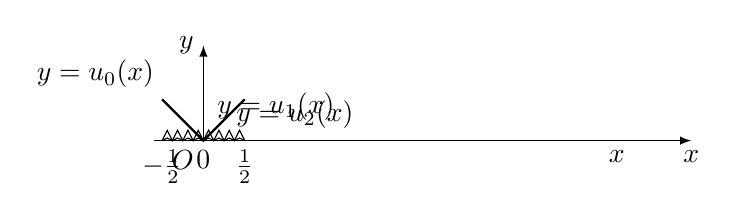
\begin{tikzpicture}[>=latex, scale=1.05]
    \draw[->] (-0.60,0) -- (5.90,0) node[below] {$x$};
    \draw[->] (0,0) -- (0,1.15) node[left] {$y$};
    \node[below left] at (0,0) {$O$};
    % u_0 = |x|（一个 V）
    \draw[thick] (-0.50,0.50) -- (0,0) -- (0.50,0.50);
    \node[above left] at (-0.48,0.52) {$y=u_{0}(x)$};
    \node[below] at (-0.50,0) {$-\frac{1}{2}$};
    \node[below] at (0,0) {$0$};
    \node[below] at (0.50,0) {$\frac{1}{2}$};
    \node[below] at (5.00,0) {$x$};
    % u_1：周期 1/4、高 1/8 的细齿
    \draw[thin] (-0.50,0) -- (-0.4375,0.125) -- (-0.375,0) -- (-0.3125,0.125) -- (-0.25,0)
      -- (-0.1875,0.125) -- (-0.125,0) -- (-0.0625,0.125) -- (0,0)
      -- (0.0625,0.125) -- (0.125,0) -- (0.1875,0.125) -- (0.25,0)
      -- (0.3125,0.125) -- (0.375,0) -- (0.4375,0.125) -- (0.50,0);
    \node[above right] at (0.05,0.13) {$y=u_{1}(x)$};
    % u_2：周期 1/16、高 1/32（只画 4 个齿示意）
    \draw[thin] (-0.50,0) -- (-0.4375,0.03125) -- (-0.375,0) -- (-0.3125,0.03125) -- (-0.25,0)
      -- (-0.1875,0.03125) -- (-0.125,0) -- (-0.0625,0.03125) -- (0,0)
      -- (0.0625,0.03125) -- (0.125,0) -- (0.1875,0.03125) -- (0.25,0)
      -- (0.3125,0.03125) -- (0.375,0) -- (0.4375,0.03125) -- (0.50,0);
    \node[above right] at (0.28,0.033) {$y=u_{2}(x)$};
  \end{tikzpicture}
  \caption{锯齿形函数 $u_{k}(x)=\frac{1}{4^{k}}u_{0}(4^{k}x)$}\label{fig:13.2.5}
\end{figure}

显然, $\forall s\in\mathbb{Z}$, $u_{0}(x)$ 在 $\left[\frac{s}{2},\frac{s+1}{2}\right]$ 上是线性的, 因此, $u_{k}(x)$ 在 $\left[\frac{s}{2\cdot4^{k}},\frac{s+1}{2\cdot4^{k}}\right]$ 上是线性的. 从而每个 $u_{k}(x)$ 都是锯齿形函数, 其齿随 $k$ 增大而变细. 令
\[
  f(x)=\sum_{k=0}^{\infty}u_{k}(x),\quad x\in(-\infty,+\infty).
\]
因为 $|u_{k}(x)|\leqslant\frac{1}{2}\cdot\frac{1}{4^{k}}$, 故由 Weierstrass 判别法, $\sum_{k=1}^{\infty}u_{k}(x)$ 在 $(-\infty,+\infty)$ 上一致收敛. 再由 $u_{k}(x)$ 连续 ($k\in\mathbb{N}$), 根据定理~\ref{thm:13.2.1p} 知, $f(x)=\sum_{k=0}^{\infty}u_{k}(x)$ 在 $(-\infty,+\infty)$ 上处处连续.

下面证明 $f(x)$ 在 $(-\infty,+\infty)$ 上处处不可导.

任取 $x_{0}\in\mathbb{R}$, 记 $[2\cdot4^{n}x_{0}]=s_{n}$, 则
\[
  s_{n}\leqslant2\cdot4^{n}x_{0}<s_{n}+1\Leftrightarrow\frac{s_{n}}{2\cdot4^{n}}\leqslant x_{0}<\frac{s_{n}+1}{2\cdot4^{n}},
\]
取 $x_{n}\in\left[\frac{s_{n}}{2\cdot4^{n}},\frac{s_{n}+1}{2\cdot4^{n}}\right]$, 使得
\[
  \left|x_{n}-x_{0}\right|=\frac{1}{2}\cdot\frac{1}{2\cdot4^{n}}=\frac{1}{4^{n+1}}
\]
(\cref{fig:13.2.6}).

\begin{figure}[htbp]
  \centering
  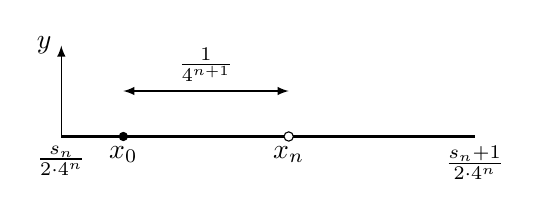
\begin{tikzpicture}[>=latex, scale=1.05]
    \draw[thick] (0,0) -- (5.00,0);
    \draw[->] (0,0) -- (0,1.10) node[left] {$y$};
    \fill (0.75,0) circle (1.6pt);
    \draw[fill=white] (2.75,0) circle (1.6pt);
    \node[below] at (0.75,0) {$x_{0}$};
    \node[below] at (2.75,0) {$x_{n}$};
    \draw[<->] (0.75,0.55) -- (2.75,0.55);
    \node[above] at (1.75,0.55) {$\frac{1}{4^{n+1}}$};
    \node[below] at (0,0) {$\frac{s_{n}}{2\cdot4^{n}}$};
    \node[below] at (5.00,0) {$\frac{s_{n}+1}{2\cdot4^{n}}$};
  \end{tikzpicture}
  \caption{取点 $x_{0}$ 与 $x_{n}$ 的位置}\label{fig:13.2.6}
\end{figure}

\[
  \lim_{n\to+\infty}x_{n}=x_{0}.
\]
于是对某个 $n\in\mathbb{N}$, 当 $k>n$ 时, 有
\[
  \begin{aligned}
    u_{k}(x_{n})&=u_{k}\left(x_{0}\pm\frac{1}{4^{n+1}}\right)=u_{k}\left(x_{0}+\frac{1}{4^{k}}\cdot4^{k-(n+1)}\right)\\
    &\xlongequal{\frac{1}{4^{k}}\text{ 为 }u_{k}\text{ 的周期}}u_{k}(x_{0}),
  \end{aligned}
\]
由此得到
\[
  \begin{aligned}
    \frac{f(x_{n})-f(x_{0})}{x_{n}-x_{0}}&=\sum_{k=0}^{\infty}\frac{u_{k}(x_{n})-u_{k}(x_{0})}{x_{n}-x_{0}}=\sum_{k=0}^{n}\frac{u_{k}(x_{n})-u_{k}(x_{0})}{x_{n}-x_{0}}\\
    &=\sum_{k=0}^{n}(\pm1)=\begin{cases}
      \text{偶数}, & n\text{ 为奇数},\\
      \text{奇数}, & n\text{ 为偶数}
\end{cases}
  \end{aligned}
\]
(当 $k\leqslant n$ 时, $\left[\frac{s_{n}}{2\cdot4^{n}},\frac{s_{n}+1}{2\cdot4^{n}}\right]\subset\left[\frac{s_{k}}{2\cdot4^{k}},\frac{s_{k}+1}{2\cdot4^{k}}\right]$, 而 $u_{k}(x)$ 在 $\left[\frac{s_{k}}{2\cdot4^{k}},\frac{s_{k}+1}{2\cdot4^{k}}\right]$ 中是线性的. 因此, 在 $\left[\frac{s_{n}}{2\cdot4^{n}},\frac{s_{n}+1}{2\cdot4^{n}}\right]$ 上也是线性的. 现 $x_{0},x_{n}\in\left[\frac{s_{n}}{2\cdot4^{n}},\frac{s_{n}+1}{2\cdot4^{n}}\right]$, 所以 $\frac{u_{k}(x_{n})-u_{k}(x_{0})}{x_{n}-x_{0}}=\pm1$.)

令 $n\to+\infty$, 显然有
\[
  \lim_{n\to+\infty}\frac{f(x_{n})-f(x_{0})}{x_{n}-x_{0}}
\]
不存在, 从而 $f(x)$ 在 $x_{0}$ 不可导. 由 $x_{0}$ 的任取性知, $f(x)$ 在 $(-\infty,+\infty)$ 上处处不可导.

\begin{example}[填满正方形的连续曲线]\label{ex:13.2.15}
1890 年, Peano 构造出一条连续曲线, 它将整个正方形填满了. 这一事实就像处处连续处处不可导的函数那样令人不可思议. 下面介绍的例子是 Schoenberg 于 1938 年提出的, 它也需依靠无穷级数来完成.
\end{example}

我们要构造一条连续曲线 $(x,y)=(x(t),y(t))$, $t\in[0,1]$. 当 $t$ 走遍了 $[0,1]$ 时, $(x(t),y(t))$ 连续地走遍正方形 $[0,1]\times[0,1]$ 中每一点. 为此, 在 $[0,1]$ 上定义函数 $\varphi$ 如下:
\[
  \varphi(t)=\begin{cases}
    0, & t\in\left[0,\frac{1}{3}\right],\\
    3t-1, & t\in\left(\frac{1}{3},\frac{2}{3}\right),\\
    1, & t\in\left[\frac{2}{3},1\right].
\end{cases}
\]
然后再将 $\varphi(t)$ 延拓为整个数轴上周期为 $2$ 的偶函数 (\cref{fig:13.2.7}), 即让 $\varphi(t)$ 满足:
\[
  \varphi(t)=\varphi(-t),\quad\varphi(t+2)=\varphi(t),\quad t\in(-\infty,+\infty).
\]

\begin{figure}[htbp]
  \centering
  \begin{tikzpicture}[>=latex, scale=1.10]
    \draw[->] (-0.60,0) -- (8.90,0) node[below] {$x$};
    \draw[->] (0,0) -- (0,2.30) node[left] {$y$};
    \node[below left] at (0,0) {$O$};
    \node[left] at (0,1.90) {$1$};
    \draw[thick] (0,0) -- (1.33,0) -- (2.67,1.90) -- (5.33,1.90) -- (6.67,0) -- (8.00,0);
    \node[below] at (1.33,0) {$\frac{1}{3}$};
    \node[below] at (2.67,0) {$\frac{2}{3}$};
    \node[below] at (5.33,0) {$\frac{4}{3}$};
    \node[below] at (6.67,0) {$\frac{5}{3}$};
    \node[below] at (8.00,0) {$2$};
    \node[above right] at (3.40,1.90) {$y=\varphi(t)$};
  \end{tikzpicture}
  \caption{$\varphi(t)$ 的周期为 $2$ 的偶延拓}\label{fig:13.2.7}
\end{figure}

现在令
\[
  (x(t),y(t))=\biggl(\sum_{n=1}^{\infty}\frac{\varphi(3^{2n-2}t)}{2^{n}},\sum_{n=1}^{\infty}\frac{\varphi(3^{2n-1}t)}{2^{n}}\biggr),\quad t\in[0,1].
\]

这是一条能填满正方形 $[0,1]\times[0,1]$ 的连续曲线.

由于 $0\leqslant\varphi(t)\leqslant1$, 所以 $\sum_{n=1}^{\infty}\frac{1}{2^{n}}$ 是上面两个函数级数的优级数, 根据 Weierstrass 判别法, 得
\[
  x(t)=\sum_{n=1}^{\infty}\frac{\varphi(3^{2n-2}t)}{2^{n}}\quad\text{与}\quad y(t)=\sum_{n=1}^{\infty}\frac{\varphi(3^{2n-1}t)}{2^{n}}
\]
在 $[0,1]$ 上都一致收敛, 根据定理~\ref{thm:13.2.1p}, $x(t)$ 与 $y(t)$ 都为 $[0,1]$ 上的连续函数, 所以, $(x(t),y(t))$ 是一条连续曲线. 余下的需证它填满了整个正方形 $[0,1]\times[0,1]$. 为此, 任取 $(a,b)\in[0,1]\times[0,1]$, 并且用二进位小数表示 $a,b$ 为
\[
  a=\sum_{n=1}^{\infty}\frac{a_{n}}{2^{n}},\quad b=\sum_{n=1}^{\infty}\frac{b_{n}}{2^{n}},
\]
这里 $a_{n},b_{n}$ 都只取 $0,1$ 中某一个值, 将 $\{a_{n}\}$, $\{b_{n}\}$ 交错排列为
\[
  a_{1},b_{1},a_{2},b_{2},\cdots,a_{n},b_{n},\cdots,
\]
并重新记为
\[
  \eta_{1},\eta_{2},\cdots,\eta_{2n-1},\eta_{2n},\cdots,
\]
其中 $\eta_{2n-1}=a_{n}$, $\eta_{2n}=b_{n}$, $n=1,2,\cdots$, 于是
\[
  0\leqslant\eta=\sum_{n=1}^{\infty}\frac{2\eta_{n}}{3^{n}}\leqslant2\sum_{n=1}^{\infty}\frac{1}{3^{n}}=1,
\]
即 $\eta\in[0,1]$. 我们证 $(x(\eta),y(\eta))=(a,b)$. 事实上, 对于固定的 $k=0,1,2,\cdots$, 有
\[
  3^{k}\eta=3^{k}\sum_{n=1}^{\infty}\frac{2\eta_{n}}{3^{n}}=2\sum_{n=1}^{k}3^{k-n}\eta_{n}+\frac{2}{3}\eta_{k+1}+2\sum_{n=k+2}^{\infty}\frac{\eta_{n}}{3^{n-k}}.
\]
容易看出, 右边第 1 个和式是 $2$ 的整倍数, 记为 $2m$. 若将第 3 个和式记为 $\alpha_{k}$, 则
\[
  0\leqslant\alpha_{k}\leqslant2\sum_{n=k+2}^{\infty}\frac{1}{3^{n-k}}=\frac{1}{3}.
\]
这样便有
\[
  3^{k}\eta=2m+\frac{2}{3}\eta_{k+1}+\alpha_{k}.
\]
由于 $\varphi(t)$ 是以 $2$ 为周期的周期函数, 所以
\[
  \begin{aligned}
    \varphi(3^{k}\eta)&=\varphi\left(2m+\frac{2}{3}\eta_{k+1}+\alpha_{k}\right)\\
    &=\varphi\left(\frac{2}{3}\eta_{k+1}+\alpha_{k}\right)=\begin{cases}
      \varphi(\alpha_{k})=0=\eta_{k+1}, & \eta_{k+1}=0,\\
      \varphi\left(\frac{2}{3}+\alpha_{k}\right)=1=\eta_{k+1}, & \eta_{k+1}=1
\end{cases}\\
    &=\eta_{k+1},
  \end{aligned}
\]
其中 $\eta_{k+1}=1$ 时, $\frac{2}{3}\leqslant\frac{2}{3}\eta_{k+1}+\alpha_{k}\leqslant\frac{2}{3}\cdot1+\frac{1}{3}=1$. 于是
\[
  x(\eta)=\sum_{n=1}^{\infty}\frac{\varphi(3^{2n-2}\eta)}{2^{n}}=\sum_{n=1}^{\infty}\frac{\eta_{2n-1}}{2^{n}}=\sum_{n=1}^{\infty}\frac{a_{n}}{2^{n}}=a,
\]
\[
  y(\eta)=\sum_{n=1}^{\infty}\frac{\varphi(3^{2n-1}\eta)}{2^{n}}=\sum_{n=1}^{\infty}\frac{\eta_{2n}}{2^{n}}=\sum_{n=1}^{\infty}\frac{b_{n}}{2^{n}}=b.
\]
这就证明了连续曲线 $(x(t),y(t))$ 的确填满了整个正方形 $[0,1]\times[0,1]$.

\begin{remark}\label{rem:13.2.2}
注意映射 $F\colon[0,1]\to[0,1]\times[0,1]$, $t\to F(t)=(x(t),y(t))$ 肯定不是一一映射, 当然更不是同胚映射. 这表明: 必有 $t_{1},t_{2}\in[0,1]$, $t_{1}\neq t_{2}$, 但 $F(t_{1})=(x(t_{1}),y(t_{1}))=(x(t_{2}),y(t_{2}))=F(t_{2})$, 称它为重点.

事实上, 若映射 $F$ 为一一映射, 根据\extref{定理 7.3.10} 知, 该映射必为同胚映射. 从而也为同胚. 而 $[0,1]\setminus\left\{\frac{1}{2}\right\}=\left[0,\frac{1}{2}\right)\cup\left(\frac{1}{2},1\right]$ 不连通, 而 $[0,1]\times[0,1]\setminus F\left(\frac{1}{2}\right)$ 连通, 这与连通为同胚不变性相矛盾.

不难看出, 利用上面的方法, 我们还能构造出填满整个立方体 $[0,1]\times[0,1]\times[0,1]$ 的空间连续曲线. 请读者证明, 空间连续函数
\[
  F(t)=(x(t),y(t),z(t))=\left(\sum_{n=1}^{\infty}\frac{\varphi(3^{3n-3}t)}{2^{n}},\sum_{n=1}^{\infty}\frac{\varphi(3^{3n-2}t)}{2^{n}},\sum_{n=1}^{\infty}\frac{\varphi(3^{3n-1}t)}{2^{n}}\right)
\]
便能填满整个立方体 $[0,1]\times[0,1]\times[0,1]$. 同样 $F\colon[0,1]\to[0,1]\times[0,1]\times[0,1]$ 也不是一一映射, 即上述空间连续曲线必有重点.
\end{remark}

上述例~\ref{ex:13.2.14} 与例~\ref{ex:13.2.15} 两个例子的魅力不仅在于它们提示了两件令人感到惊异的事实. 还在于它们是近 20 年来正蓬勃兴起并且很有应用前景的一门新兴学科 ``分形几何'' 中所谓 ``分形集'' 的典型例子.

\begin{exblock}{练习题 13.2}
\begin{enumerate}
  \item 确定下列函数的存在域, 并研究它们的连续性:
  \begin{enumerate}
    \item $f(x)=\displaystyle\sum_{n=1}^{\infty}\left(x+\frac{1}{n}\right)^{n}$;
    \item $f(x)=\displaystyle\sum_{n=1}^{\infty}\frac{x+(-1)^{n}n}{x^{2}+n^{2}}$.
  \end{enumerate}
  \item 证明: 函数
  \[
    f(x)=\sum_{n=1}^{\infty}\frac{\cos nx}{n^{4}}
\]
  在 $(-\infty,+\infty)$ 中有二阶连续导函数, 并计算 $f''(x)$.
  \item 设 $f(x)=\sum_{n=1}^{\infty}n\mathrm{e}^{-nx}$ ($x>0$), 计算 $\int_{\ln2}^{\ln3}f(x)\mathrm{d}x$.
  \item 设 $f(x)=\sum_{n=1}^{\infty}\left(\frac{x}{1+2x}\right)^{n}\cos\frac{n\pi}{x}$, 计算: $\lim\limits_{x\to1}f(x)$, $\lim\limits_{x\to+\infty}f(x)$.
  \item 已知 $\sum_{n=1}^{\infty}\frac{(-1)^{n-1}}{n}=\ln2$, 证明: $\lim\limits_{x\to1}\sum_{n=1}^{\infty}\frac{(-1)^{n-1}}{n^{x}}=\ln2$.
  \item 证明: $f(x)=\sum_{n=1}^{\infty}\left(x+\frac{1}{n}\right)^{n}$ 在 $(-1,1)$ 内连续.
  \item 证明: $\sum_{n=1}^{\infty}\frac{x}{(1+x^{2})^{n}}$ 在 $(0,+\infty)$ 内非一致收敛.
\end{enumerate}
\end{exblock}

\begin{exblock}{思考题 13.2}
\begin{enumerate}
  \item 设 $E$ 为 $(-\infty,+\infty)$ 中的一点集, $x_{0}$ 为 $E$ 的广义聚点 (即 $x_{0}$ 可为实数或 $\pm\infty$, $x_{0}$ 的任何开邻域中必含 $E$ 中异于 $x_{0}$ 的点). 如果函数项级数 $\sum_{n=1}^{\infty}u_{n}(x)$ 在 $E$ 上一致收敛, 且 $\lim\limits_{n\to+\infty}u_{n}(x)=a_{n}$, $n=1,2,\cdots$. 证明:

  (1) $\sum_{n=1}^{\infty}a_{n}$ 收敛;

  (2) $\lim\limits_{x\to x_{0}}\sum_{n=1}^{\infty}u_{n}(x)=\sum_{n=1}^{\infty}a_{n}=\sum_{n=1}^{\infty}\lim\limits_{x\to x_{0}}u_{n}(x)$.
  \item 利用 $\sum_{n=1}^{\infty}\frac{1}{n^{2}}=\frac{\pi^{2}}{6}$, 证明:
  \[
    \lim_{x\to1}\sum_{n=1}^{\infty}\frac{x^{n}(1-x)}{n(1-x^{2n})}=\frac{\pi^{2}}{12}.
\]
  \item 设函数项级数 $\sum_{n=1}^{\infty}u_{n}(x)$ 满足下列条件:

  (1) $\sum_{n=1}^{\infty}u_{n}(x)$ 在 $(x_{0}-\delta,x_{0}+\delta)$ 中收敛于 $f(x)$;

  (2) 函数项级数的每一项 $u_{n}(x)$ 在 $x=x_{0}$ 处可导;

  (3) 函数项级数 $\sum_{n=1}^{\infty}\frac{u_{n}(x)-u_{n}(x_{0})}{x-x_{0}}$ 在 $0<|x-x_{0}|<\delta$ 中一致收敛.

  则 $f(x)$ 在 $x_{0}$ 处可导, 且 $f'(x_{0})=\sum_{n=1}^{\infty}u_{n}'(x_{0})$.
  \item 在 $(0,1)$ 中任取一数列 $\{a_{n}\}$, 其中两两不相同. 证明: 函数
  \[
    f(x)=\sum_{n=1}^{\infty}\frac{|x-a_{n}|}{2^{n}}
\]
  在 $(0,1)$ 中连续, 且在 $x=a_{n}$ ($n=1,2,\cdots$) 处都不可导, 而在 $(0,1)$ 中其他点处都可导.
  \item 设 $\{x_{n}\}$ 为区间 $[0,1)$ 中的全体有理数, 对任意 $x\in(0,1)$, 定义
  \[
    f(x)=\sum_{x_{n}<x}\frac{1}{2^{n}}.
\]
  令
  \[
    g_{n}(x)=\begin{cases}
      0, & x\leqslant x_{n},\\
      \frac{1}{2^{n}}, & x>x_{n},
\end{cases}
\]
  证明:

  (1) 级数 $\sum_{n=1}^{\infty}g_{n}(x)$ 在 $(0,1)$ 上一致收敛于 $f(x)$;

  (2) $\int_{0}^{1}f(x)\mathrm{d}x=\sum_{n=1}^{\infty}\frac{1-x_{n}}{2^{n}}$.
  \item 设 $\{x_{n}\}$ 为 $(0,1)$ 内的一个数列, 且 $x_{i}\neq x_{j}$ ($i\neq j$), 证明
  \[
    f(x)=\sum_{n=1}^{\infty}\frac{\operatorname{sgn}(x-x_{n})}{2^{n}}
\]
  在 $(0,1)$ 内一致收敛; $f(x)$ 在 $(0,1)\setminus\{x_{n}\mid n=1,2,\cdots\}$ 中每一点处连续, 而在每个 $x_{n}$ ($n=1,2,\cdots$) 处不连续.
  \item 证明: $f(x)=\sum_{n=1}^{\infty}n\mathrm{e}^{-nx}$ 在 $(0,+\infty)$ 内收敛, 但不一致收敛, 而和函数在 $(0,+\infty)$ 内无穷次可导.
  \item 设 $h(x)$, $f_{n}'(x)$ 在 $[a,b]$ 上连续, $n=1,2,\cdots$, 又对 $[a,b]$ 中任意的 $x_{1},x_{2}$ 与正整数 $n$ 有
  \[
    \left|f_{n}(x_{1})-f_{n}(x_{2})\right|\leqslant\frac{M}{n}|x_{1}-x_{2}|,
\]
  其中 $M\geqslant0$ 为常数. 证明:

  (1) $f_{n}'(x)\rightrightarrows0$, $x\in[a,b]$, $n\to+\infty$;

  (2) $\lim\limits_{n\to+\infty}\int_{a}^{b}h(x)f_{n}'(x)\mathrm{d}x=0$.
\end{enumerate}
\end{exblock}

% ==================================================================
%  徐森林、金亚东、薛春华《数学分析》（第三册）
%  复习题 13
%  源：原书印刷页 123-129（PDF 物理页 129-135）
%  底本：PaddleOCR-VL-1.6，见 chapters/_ch13_13_2_raw.md 末尾
%  约定：只用 exblock，不设 section（故不入目录）
%  全 27 题题面照录；订正说明见 tools/_make_ch13_ex.py 头部
% ==================================================================

\begin{exblock}{复习题 13}
\begin{enumerate}
  \item 设函数 $f(x)$ 在 $x=0$ 的邻域里有二阶连续导函数, 且 $f(0)=0$, $0<f'(0)<1$. 如果 $f_{n}(x)$ 为 $f(x)$ 的 $n$ 次复合, 即
  \[
    f_{n}=\underbrace{f\circ f\circ\cdots\circ f}_{n\text{ 次}}.
\]
  证明: 函数项级数 $\sum_{n=1}^{\infty}f_{n}(x)$ 在 $x=0$ 的邻域里一致收敛.
  \item 证明: 函数项级数
  \[
    \sum_{n=1}^{\infty}\frac{x^{n}}{1+x+x^{2}+\cdots+x^{2n-1}}\cos nx
\]
  在 $(0,1]$ 中一致收敛.
  \item 设 $\sum_{n=1}^{\infty}u_{n}(x)$ 在 $[a,b]$ 上收敛, 如果
  \[
    |S_{n}(x)|=\left|\sum_{k=1}^{n}u_{k}(x)\right|\leqslant M,\quad a\leqslant x\leqslant b,\ n=1,2,\cdots,
\]
  就称 $\sum_{n=1}^{\infty}u_{n}(x)$ 在 $[a,b]$ 上有界收敛.

  设 $\sum_{n=1}^{\infty}u_{n}(x)$ 在 $[a,b]$ 上有界收敛, 且对任意 $\delta>0$ 及 $c\in(a,b)$, $\sum_{n=1}^{\infty}u_{n}(x)$ 在 $[a,c-\delta]$ 与 $[c+\delta,b]$ 上一致收敛. 如果 $u_{n}(x)$ ($n=1,2,\cdots$) 在 $[a,b]$ 上 Riemann 可积, 则 $\sum_{n=1}^{\infty}u_{n}(x)$ 也在 $[a,b]$ 上 Riemann 可积, 且
  \[
    \int_{a}^{b}\left(\sum_{n=1}^{\infty}u_{n}(x)\right)\mathrm{d}x=\sum_{n=1}^{\infty}\int_{a}^{b}u_{n}(x)\mathrm{d}x.
\]
  \item 设函数项级数 $\sum_{n=1}^{\infty}u_{n}(x)$ 满足下列条件:

  (1) 广义积分 $\int_{a}^{+\infty}u_{n}(x)\mathrm{d}x$ 收敛, $n=1,2,\cdots$;

  (2) 函数项级数 $\sum_{n=1}^{\infty}u_{n}(x)$ 在区间 $[a,b]$ 上一致收敛, 这里 $b$ 是大于 $a$ 的任何实数;

  (3) 函数项级数 $\sum_{n=1}^{\infty}\int_{a}^{x}u_{n}(t)\mathrm{d}t$ 在 $[a,+\infty)$ 上一致收敛.

  则 $\int_{a}^{+\infty}\left(\sum_{n=1}^{\infty}u_{n}(x)\right)\mathrm{d}x$ 与 $\sum_{n=1}^{\infty}\int_{a}^{+\infty}u_{n}(x)\mathrm{d}x$ 都收敛, 且
  \[
    \int_{a}^{+\infty}\left(\sum_{n=1}^{\infty}u_{n}(x)\right)\mathrm{d}x=\sum_{n=1}^{\infty}\int_{a}^{+\infty}u_{n}(x)\mathrm{d}x.
\]
  \item 设 $r_{1},r_{2},\cdots$ 为 $[0,1]$ 中的有理数. 证明: 函数
  \[
    f(x)=\sum_{n=1}^{\infty}\frac{|x-r_{n}|}{3^{n}}\quad(0\leqslant x\leqslant1)
\]
  连续, 且在无理点可导, 但在有理点不可导.
  \item 设 $K(x,t)$ 在 $[a,b]\times[a,b]$ 上连续, $u_{0}(x)$ 在 $[a,b]$ 上连续, 且对任意 $x\in[a,b]$, 令
  \[
    u_{n}(x)=\int_{a}^{x}K(x,t)u_{n-1}(t)\mathrm{d}t,\quad n=1,2,\cdots,
\]
  证明: 函数列 $\{u_{n}(x)\}$ 在 $[a,b]$ 上一致收敛.
  \item 设 $f(x)$ 在 $(-\infty,+\infty)$ 内连续; 当 $x\neq0$ 时, 有 $|f(x)|<|x|$. 令
  \[
    \begin{aligned}
      f_{1}(x)&=f(x),\quad f_{2}(x)=f(f_{1}(x))=f\circ f(x),\\
      f_{n}(x)&=f(f_{n-1}(x))=\underbrace{f\circ f\circ\cdots\circ f}_{n\text{ 个}}(x),\ \cdots
    \end{aligned}
\]
  证明: $\{f_{n}(x)\}$ 在 $[-A,A]$ 上一致收敛.
  \item 设 $\alpha_{n}>0$, $\lim\limits_{n\to+\infty}\alpha_{n}=0$, $|u_{n}(x)|\leqslant\alpha_{n}$, $\forall x\in I$, 且 $u_{i}(x)u_{j}(x)=0$ ($i\neq j$). $\forall x\in I\subset\mathbb{R}$.

  证明: $\sum_{n=1}^{\infty}u_{n}(x)$ 在 $I$ 上一致收敛.
  \item 设 $\{u_{n}(x)\}$ 为 $[a,b]$ 上的可导函数列, 且在 $[a,b]$ 上有
  \[
    \left|\sum_{k=1}^{n}u_{k}'(x)\right|\leqslant C,
\]
  其中 $C$ 是不依赖 $x$ 与 $n$ 的正数. 证明: 若 $\sum_{n=1}^{\infty}u_{n}(x)$ 在 $[a,b]$ 上收敛, 则必为一致收敛.
  \item 设函数列 $f_{0}(x)$, $f_{1}(x)$, $\cdots$, $f_{n}(x)$, $\cdots$ 在 $I\subseteq\mathbb{R}$ 上有定义, 且满足:
  \[
    |f_{0}(x)|\leqslant M,\quad x\in I,
\]
  \[
    \sum_{n=0}^{m}|f_{n}(x)-f_{n+1}(x)|\leqslant M,\quad m=0,1,2,\cdots,\ x\in I,
\]
  其中 $M$ 为常数. 证明: 如果级数 $\sum_{n=0}^{\infty}b_{n}$ 收敛, 则函数项级数 $\sum_{n=0}^{\infty}b_{n}f_{n}(x)$ 必在 $I$ 上一致收敛.
  \item 证明: 函数项级数
  \[
    \sum_{n=1}^{\infty}\frac{1}{n}\left[\mathrm{e}^{x}-\left(1+\frac{x}{n}\right)^{n}\right]
\]
  在任意有限区间 $[a,b]$ 上一致收敛, 但在 $(0,+\infty)$ 上非一致收敛.
  \item 证明: $\sum_{n=1}^{\infty}(1-x)\frac{x^{n}}{1-x^{2n}}\sin nx$ 在 $\left(\frac{1}{2},1\right)$ 内一致收敛.
  \item 证明:

  (1) 函数列 $\left(1+\frac{x}{n}\right)^{n}$ ($n=1,2,\cdots$) 在 $[0,1]$ 上一致收敛于 $\mathrm{e}^{x}$;

  (2) 函数列 $f_{n}(x)=\dfrac{1}{\mathrm{e}^{\frac{x}{n}}+\left(1+\frac{x}{n}\right)^{n}}$ ($n=1,2,\cdots$) 在 $[0,1]$ 上一致收敛于 $\dfrac{1}{1+\mathrm{e}^{x}}$;

  (3) $\lim\limits_{n\to+\infty}\int_{0}^{1}\frac{\mathrm{d}x}{\mathrm{e}^{\frac{x}{n}}+\left(1+\frac{x}{n}\right)^{n}}=1+\ln\frac{2}{1+\mathrm{e}}$.
  \item 设 $\{r_{n}\}$ 为区间 $[0,1]$ 上全体有理数组成的数列, $u_{n}(x)$ 在 $[0,1]$ 上一致地满足 Lipschitz 条件, 即 $\exists L>0$, 使得 $\forall x_{1},x_{2}\in[0,1]$ 有
  \[
    \left|u_{n}(x_{1})-u_{n}(x_{2})\right|\leqslant L|x_{1}-x_{2}|,\ \forall n\in\mathbb{N}.
\]
  又设 $u_{n}(0)=0$, $u_{n}(x)$ 只在 $r_{n}$ 处不可导, 而在 $[0,1]$ 的其他点处可导 ($n=1,2,\cdots$). 证明:

  (1) $f(x)=\sum_{n=1}^{\infty}\frac{u_{n}(x)}{2^{n}}$ 在 $[0,1]$ 上连续;

  (2) $f(x)$ 在 $[0,1]$ 的有理点处不可导, 而在无理点处可导, 且导数
  \[
    f'(x)=\sum_{n=1}^{\infty}\frac{u_{n}'(x)}{2^{n}}.
\]
  \item 设 $g(x)$ 与 $f_{n}(x)\geqslant0$ ($n=1,2,\cdots$) 在 $[a,b]$ 上有界可积, 且 $\forall c\in(a,b)$, 有
  \[
    f_{n}(x)\rightrightarrows0,\ x\in[c,b],\quad n\to+\infty;
\]
  \[
    \lim_{n\to+\infty}\int_{a}^{b}f_{n}(x)\mathrm{d}x=1,\quad\lim_{x\to a^{+}}g(x)=A.
\]
  证明: $\lim\limits_{n\to+\infty}\int_{a}^{b}g(x)f_{n}(x)\mathrm{d}x=A$.
  \item 证明: 函数项级数 $\sum_{n=1}^{\infty}x^{2n}\ln x$ 在 $(0,1)$ 内不一致收敛, 但在 $[0,1]$ 上可逐项积分.
  \item 设 $\{f_{n}(x)\}$ 为 $(-\infty,+\infty)$ 上定义并且连续的函数列. 试构造一个在 $(-\infty,+\infty)$ 上有界、连续的函数 $f(x)$, 使得 $f(x)=0\Leftrightarrow f_{n}(x)=0$, $n=1,2,\cdots$.
  \item 设 $f_{n}(x)$ ($n=1,2,\cdots$) 在 $[0,1]$ 上连续, 并且 $f_{n}(x)\geqslant f_{n+1}(x)$, $\forall x\in[0,1]$, $n=1,2,\cdots$. 如果 $f_{n}(x)$ 在 $[0,1]$ 上收敛于 $f(x)$. 证明: $f(x)$ 在 $[0,1]$ 上达到最大值. 举例说明, 上述 $f(x)$ 在 $[0,1]$ 上未必达到最小值.
  \item 设 $f_{n}(x)$ ($n=1,2,\cdots$) 在 $[a,b]$ 上连续可导, 且 $\max\limits_{a\leqslant x\leqslant b}|f_{n}'(x)|\leqslant M$ ($n=1,2,\cdots$). 又 $\{f_{n}(x)\}$ 在 $[a,b]$ 上每一点处收敛. 证明: $\{f_{n}(x)\}$ 在 $[a,b]$ 上一致收敛. 如果 ``连续可导'' 改为 ``可导'', 上述结论是否仍正确?
  \item 设 $\{f_{n}(x)\}$ 是定义在 $[a,b]$ 上的连续函数列, 且 $\{f_{n}(x)\}$ 在 $[a,b]$ 上一致收敛于 $f(x)$. 又 $\{x_{n}\}\subset[a,b]$, 且 $x_{n}\to x_{0}$ ($n\to+\infty$), 证明: $\lim\limits_{n\to+\infty}f_{n}(x_{n})=f(x_{0})$.
  \item (Dini 定理) 设 $\{f_{n}(x)\}$ 为 $[a,b]$ 上的连续函数列, 且对任意 $x\in[a,b]$, 有 $f_{n}(x)\leqslant f_{n+1}(x)$. 证明: 如果 $\{f_{n}(x)\}$ 收敛于连续函数 $f(x)$, 则 $\{f_{n}(x)\}$ 在 $[a,b]$ 上必一致收敛于 $f(x)$.
  \item 设对每一个 $n$, $f_{n}(x)$ 为 $[a,b]$ 上的单调函数. 证明: 如果函数列 $\{f_{n}(x)\}$ 在 $[a,b]$ 上收敛于连续函数 $f(x)$, 则 $\{f_{n}(x)\}$ 在 $[a,b]$ 上必一致收敛于 $f(x)$.
  \item 设每个函数 $u_{n}(x)$ ($n=1,2,\cdots$) 都在点 $x=c$ 处连续, 但 $\sum_{n=1}^{\infty}u_{n}(c)$ 发散. 证明: $\forall\delta>0$, 级数 $\sum_{n=1}^{\infty}u_{n}(x)$ 在 $(c,c+\delta)$ 内不一致收敛.
  \item 设 $\{u_{n}(x)\}$ 是 $[a,b]$ 上正的单调减 ($u_{n+1}(x)\leqslant u_{n}(x)$) 且收敛于 $0$ 的函数列, 每个 $u_{n}(x)$ 都是 $[a,b]$ 上的单调增函数. 证明: 函数项级数 $\sum_{n=1}^{\infty}(-1)^{n-1}u_{n}(x)$ 在 $[a,b]$ 上一致收敛.
  \item 证明: 函数项级数 $\sum_{n=1}^{\infty}\frac{n^{2}}{\sqrt{n!}}(x^{n}+x^{-n})$ 在 $\frac{1}{2}\leqslant x\leqslant1$ 上一致收敛.
  \item 证明: Riemann $\zeta$ 函数 $\zeta(x)=\sum_{n=1}^{\infty}\frac{1}{n^{x}}$ 在 $(1,+\infty)$ 上为 $C^{\infty}$ 函数. 但它在 $(1,+\infty)$ 上不一致连续. 且 $\sum_{n=1}^{\infty}\frac{1}{n^{x}}$ 在 $(1,+\infty)$ 上非一致收敛.
  \item 设级数 $\sum_{n=1}^{\infty}a_{n}$ 收敛, 证明: Dirichlet 级数 $\sum_{n=1}^{\infty}\frac{a_{n}}{n^{x}}$ 当 $x\geqslant0$ 时一致收敛.
\end{enumerate}
\end{exblock}



% 第 14 章 幂级数、用多项式一致逼近连续函数（§14.1–§14.3 + 复习题 14）
% ==================================================================
%  徐森林、金亚东、薛春华《数学分析》（第三册）
%  第 14 章  幂级数、用多项式一致逼近连续函数
%  源：原书印刷页 129-176（PDF 物理页 = 印刷页 + 6）
% ==================================================================

\chapter{幂级数、用多项式一致逼近连续函数}\label{ch:14}

幂级数 $\sum_{n=0}^{\infty}a_{n}(x-x_{0})^{n}$ 是一类简单而重要的函数项级数. 本章将给出幂级数的重要性. 建立幂级数展开的惟一性定理与 Taylor 展开的充分条件与必要条件. 并通过例题展示了 Taylor 展开的各种方法. 最后, 证明了闭区间 $[a,b]$ 上的任何连续函数 $f$ 能用多项式函数一致逼近的 Weierstrass 定理.

% ==================================================================
%  徐森林、金亚东、薛春华《数学分析》（第三册）
%  S14.1  幂级数的重要性质
%  源：原书印刷页 129-145（PDF 物理页 135-151）
%  底本：PaddleOCR-VL-1.6，见 chapters/_ch14_14_1_raw.md
%  约定：全西文标点；行间公式用一对方括号；多行公式用 align/aligned；
%        跨册引用一律 \extref；数学模式内的中文必须包 \text{}
%  插图：图 14.1.1 原生 TikZ（禁用位图）
%  已订正的 OCR 错误与原书照录清单见 tools/_make_ch14_1a.py 头部说明
% ==================================================================
\section{幂级数的重要性质}\label{sec:14.1}

函数项级数中, 有一种简单且使用起来又方便的特殊函数项级数——幂级数. 幂级数的一般形状如下:
\[
  \sum_{n=0}^{\infty}a_{n}(x-x_{0})^{n}=a_{0}+a_{1}(x-x_{0})+\cdots+a_{n}(x-x_{0})^{n}+\cdots,
\]
其中 $a_{n}\in\mathbb{R}$, $n=1,2,\cdots$. 如果上式中 $a_{n+1}=a_{n+2}=\cdots=0$, 它就退化为一个 $n$ 次多项式. 因此, 多项式可以视作一种特殊的幂级数.

为讨论简单起见, 我们往往令 $x_{0}=0$, 只讨论形如
\[
  \sum_{n=1}^{\infty}a_{n}x^{n}=a_{0}+a_{1}x+\cdots+a_{n}x^{n}+\cdots
\]
的幂级数. 一般的情形只需作变换 $y=x-x_{0}$ 就行了.

首先关心的是 $\sum_{n=1}^{\infty}a_{n}x^{n}$ 的收敛点集. 与一般的函数项级数不同, 幂级数的收敛点集一定是一个区间 (可退化为一个点).

\begin{theorem}\label{thm:14.1.1}
设 $\sum_{n=1}^{\infty}a_{n}(x-x_{0})^{n}$ 为幂级数, $\alpha=\lim\limits_{n\to+\infty}\sqrt[n]{|a_{n}|}$, $R=\frac{1}{\alpha}=\frac{1}{\lim\limits_{n\to+\infty}\sqrt[n]{|a_{n}|}}$. 则:

(1) 当 $R=0$ ($\alpha=+\infty$) 时, 幂级数仅在 $x=x_{0}$ 这一点绝对收敛;

(2) 当 $R=+\infty$ ($\alpha=0$) 时, 幂级数在 $(-\infty,+\infty)$ 上绝对收敛;

(3) 当 $0<R<+\infty$, 时, 幂级数在 $(x_{0}-R,x_{0}+R)$ 中绝对收敛. 而在 $[x_{0}-R,x_{0}+R]$ 外 (即 $(-\infty,x_{0}-R)\cup(x_{0}+R,+\infty)$ 内) 发散.
\end{theorem}

\begin{proof}
因为
\[
  \lim_{n\to+\infty}\sqrt[n]{|a_{n}(x-x_{0})^{n}|}=\lim_{n\to+\infty}\sqrt[n]{|a_{n}|}\cdot|x-x_{0}|=\alpha\cdot|x-x_{0}|=\frac{|x-x_{0}|}{R}.
\]
根据数项级数的 Cauchy 判别法的极限形式得到:

(1) 当 $R=0$ ($\alpha=+\infty$) 时, 则 $\lim\limits_{n\to+\infty}\sqrt[n]{|a_{n}(x-x_{0})^{n}|}=+\infty>1$, $\sum_{n=1}^{\infty}a_{n}(x-x_{0})^{n}$ 发散, 因此幂级数仅当 $x=x_{0}$ 时收敛 (也是绝对收敛).

(2) 当 $R=+\infty$ ($\alpha=0$) 时, 则 $\lim\limits_{n\to+\infty}\sqrt[n]{|a_{n}(x-x_{0})^{n}|}=0<1$, 幂级数在 $(-\infty,+\infty)$ 上绝对收敛.

(3) 当 $0<R=\frac{1}{\alpha}<+\infty$ 时, 则 $\lim\limits_{n\to+\infty}\sqrt[n]{|a_{n}(x-x_{0})^{n}|}=\frac{|x-x_{0}|}{R}<1$, 即 $|x-x_{0}|<R$ 或 $x\in(x_{0}-R,x_{0}+R)$ 时, 幂级数绝对收敛. 而当 $\lim\limits_{n\to+\infty}\sqrt[n]{|a_{n}(x-x_{0})^{n}|}=\frac{|x-x_{0}|}{R}>1$, 即 $|x-x_{0}|>R$ 或 $x\in(-\infty,x_{0}-R)\cup(x_{0}+R,+\infty)$ 时, 幂级数发散.
\end{proof}

\begin{definition}\label{def:14.1.1}
称定理~\ref{thm:14.1.1} 中的 $R$ 为幂级数的收敛半径, $(x_{0}-R,x_{0}+R)$ 为幂级数的收敛区间.
\end{definition}

定理~\ref{thm:14.1.1} 实际上给出了计算收敛半径 $R$ 的公式. 为叙述简单起见, 下面只讨论 $x_{0}=0$ 的情形, 一般情形是完全类似的.

\begin{example}\label{ex:14.1.1}
计算下列幂级数的收敛半径、收敛区间、收敛点集:

(1) $\sum_{n=1}^{\infty}x^{n}$;

(2) $\sum_{n=1}^{\infty}nx^{n}$;

(3) $\sum_{n=1}^{\infty}\frac{x^{n}}{n!}$;

(4) $\sum_{n=1}^{\infty}n^{n}x^{n}$.
\end{example}

\begin{proof}
(1) $\alpha=\lim\limits_{n\to+\infty}\sqrt[n]{|a_{n}|}=\lim\limits_{n\to+\infty}\sqrt[n]{1}=\lim\limits_{n\to+\infty}1=1$, 收敛半径 $R=\frac{1}{\alpha}=1$, 收敛区间为 $(-R,R)=(-1,1)$. 由于 $\sum_{n=1}^{\infty}(-1)^{n}$ 与 $\sum_{n=1}^{\infty}1^{n}=\sum_{n=1}^{\infty}1$ 都发散, 故收敛点集也为 $(-R,R)=(-1,1)$.

(2) $\alpha=\lim\limits_{n\to+\infty}\sqrt[n]{|a_{n}|}=\lim\limits_{n\to+\infty}\sqrt[n]{|n|}=\lim\limits_{n\to+\infty}\sqrt[n]{n}=1$, 而
\[
  \sum_{n=1}^{\infty}n(-1)^{n}\quad\text{与}\quad\sum_{n=1}^{\infty}n\cdot1^{n}=\sum_{n=1}^{\infty}n
\]
都发散, 故收敛半径 $R=\frac{1}{\alpha}=1$, 收敛区间与收敛点集都为 $(-1,1)$.

(3) $\alpha=\lim\limits_{n\to+\infty}\sqrt[n]{|a_{n}|}=\lim\limits_{n\to+\infty}\sqrt[n]{\frac{1}{n!}}$ (见\extref{例 1.1.9}), 收敛半径为 $+\infty$, 收敛区间与收敛点集都为 $(-\infty,+\infty)$.

(4) $\alpha=\lim\limits_{n\to+\infty}\sqrt[n]{|a_{n}|}=\lim\limits_{n\to+\infty}\sqrt[n]{|n^{n}|}=\lim\limits_{n\to+\infty}n=+\infty$, 所以 $R=0$, 收敛半径为 $0$, 收敛区间为 $(-0,0)=\emptyset$, 收敛点集为 $\{0\}$.
\end{proof}

\begin{example}\label{ex:14.1.2}
计算幂级数 $\sum_{k=0}^{\infty}2^{k}x^{2k}$ 的收敛半径、收敛区间、收敛点集.
\end{example}

\begin{proof}
显然,
\[
  a_{n}=\begin{cases}
    2^{k}, & n=2k,\\
    0, & n=2k+1,
\end{cases}
\]
则
\[
  \alpha=\lim_{n\to+\infty}\sqrt[n]{|a_{n}|}=\lim_{n\to+\infty}\sqrt[2k]{2^{k}}=\lim_{n\to+\infty}\sqrt{2}=\sqrt{2},
\]
幂级数的收敛半径为 $R=\frac{1}{\alpha}=\frac{1}{\sqrt{2}}$, 收敛区间为 $(-R,R)=\left(-\frac{1}{\sqrt{2}},\frac{1}{\sqrt{2}}\right)$.

又因为
\[
  \sum_{k=0}^{\infty}2^{k}\left(\frac{1}{\sqrt{2}}\right)^{2k}=\sum_{k=0}^{\infty}1=+\infty,\quad\sum_{k=0}^{\infty}2^{k}\left(-\frac{1}{\sqrt{2}}\right)^{2k}=\sum_{k=0}^{\infty}1=+\infty,
\]
所以, 幂级数的收敛点集为 $\left(-\frac{1}{\sqrt{2}},\frac{1}{\sqrt{2}}\right)$.
\end{proof}

\begin{example}\label{ex:14.1.3}
计算下列幂级数的收敛半径、收敛区间、收敛点集:

(1) $\sum_{n=1}^{\infty}\frac{x^{n}}{n}$;

(2) $\sum_{n=1}^{\infty}\frac{x^{n}}{n^{2}}$.
\end{example}

\begin{proof}
(1) $\alpha=\lim\limits_{n\to+\infty}\sqrt[n]{|a_{n}|}=\lim\limits_{n\to+\infty}\frac{1}{\sqrt[n]{n}}=1$, 而
\[
  \sum_{n=1}^{\infty}\frac{(-1)^{n}}{n}\ \text{收敛},\quad\sum_{n=1}^{\infty}\frac{1^{n}}{n}=\sum_{n=1}^{\infty}\frac{1}{n}=+\infty,
\]
因此, 幂级数的收敛半径为 $1$, 收敛区间为 $(-1,1)$, 收敛点集为 $[-1,1)$.

(2) $\alpha=\lim\limits_{n\to+\infty}\sqrt[n]{|a_{n}|}=\lim\limits_{n\to+\infty}\sqrt[n]{\frac{1}{n^{2}}}=\lim\limits_{n\to+\infty}\frac{1}{(\sqrt[n]{n})^{2}}=1$, 而 $\sum_{n=1}^{\infty}\frac{(-1)^{n}}{n^{2}}$ 与 $\sum_{n=1}^{\infty}\frac{1^{n}}{n^{2}}=\sum_{n=1}^{\infty}\frac{1}{n^{2}}$ 都绝对收敛, 因此, 幂级数的收敛半径为 $1$, 收敛区间为 $(-1,1)$, 收敛点集为 $[-1,1]$.
\end{proof}

注意, 例~\ref{ex:14.1.3} 表明, 收敛区间与收敛点集不一定相同, 但是, 收敛区间一定是收敛点集的子集.

\begin{example}\label{ex:14.1.4}
求广义幂级数 $\sum_{n=0}^{\infty}\frac{1}{2n+1}\left(\frac{1-x}{1+x}\right)^{n}$ 的收敛点集.
\end{example}

\begin{proof}
设 $t=\frac{1-x}{1+x}$, 显然幂级数
\[
  \sum_{n=0}^{\infty}\frac{t^{n}}{2n+1}
\]
的收敛半径
\[
  R=\frac{1}{\alpha}=\frac{1}{\lim\limits_{n\to+\infty}\sqrt[n]{\frac{1}{2n+1}}}=\frac{1}{\lim\limits_{n\to+\infty}\left(\sqrt[2n+1]{\frac{1}{2n+1}}\right)^{\frac{2n+1}{n}}}=1.
\]
当 $t=-1$ 时, 由 Leibniz 判别法知, $\sum_{n=0}^{\infty}\frac{(-1)^{n}}{2n+1}$ 收敛;

当 $t=1$ 时, $\sum_{n=0}^{\infty}\frac{1^{n}}{2n+1}=\sum_{n=0}^{\infty}\frac{1}{2n+1}$ 发散.

因此, 幂级数 $\sum_{n=0}^{\infty}\frac{t^{n}}{2n+1}$ 的收敛点集为 $[-1,1)$. 解不等式 $-1\leqslant t<1$, 即
\[
  -1\leqslant\frac{1-x}{1+x}<1,
\]
得 $x>0$. 于是, 广义幂级数 $\sum_{n=0}^{\infty}\frac{1}{2n+1}\left(\frac{1-x}{1+x}\right)^{n}$ 的收敛点集为 $(0,+\infty)$.
\end{proof}

从定理~\ref{thm:14.1.1} 立即得到下面的定理.

\begin{theorem}[Abel]\label{thm:14.1.2}
如果幂级数 $\sum_{n=0}^{\infty}a_{n}x^{n}$ 在点 $x=x_{0}$ ($x_{0}\neq0$) 处收敛, 则它必在区间 $|x|<|x_{0}|$ 中绝对收敛. 如果 $\sum_{n=0}^{\infty}a_{n}x^{n}$ 在点 $x=x_{1}$ 处发散, 则它必在 $|x|>|x_{1}|$ 发散.
\end{theorem}

\begin{proof}
证法 1 设幂级数 $\sum_{n=1}^{\infty}a_{n}x^{n}$ 的收敛半径为 $R$, 由题设 $|x_{0}|\leqslant R$, 因而 $(-|x_{0}|,|x_{0}|)\subset(-R,R)$, 故 $\sum_{n=0}^{\infty}a_{n}x^{n}$ 在 $(-|x_{0}|,|x_{0}|)$ 中绝对收敛.

因为 $\sum_{n=0}^{\infty}a_{n}x^{n}$ 在 $x=x_{1}$ 处发散, 故 $x_{1}\notin(-R,R)$, 且 $\sum_{n=0}^{\infty}a_{n}x^{n}$ 在 $|x|>|x_{1}|$ 处发散 (\cref{fig:14.1.1}).

证法 2 因为 $\sum_{n=0}^{\infty}a_{n}x^{n}$ 在 $x_{0}$ 处收敛, 故 $a_{n}x_{0}^{n}\to0$ ($n\to+\infty$), 从而 $\{a_{n}x_{0}^{n}\}$ 有界, 记 $|a_{n}x_{0}^{n}|\leqslant M$, $\forall n\in\mathbb{N}$. 对 $|x|<|x_{0}|$, 有
\[
  |a_{n}x^{n}|=|a_{n}x_{0}^{n}|\cdot\left|\frac{x}{x_{0}}\right|^{n}\leqslant M\cdot\left|\frac{x}{x_{0}}\right|^{n}.
\]
再从 $\sum_{n=0}^{\infty}\left|\frac{x}{x_{0}}\right|^{n}$ 收敛与级数的比较判别法~\ref{thm:12.2.3}(1) 得到 $\sum_{n=0}^{\infty}|a_{n}x^{n}|$ 收敛.

如果 $\sum_{n=0}^{\infty}a_{n}x^{n}$ 在 $x_{1}$ 处发散, 则它必在 $|x|>|x_{1}|$ 发散. (反证) 假设 $\sum_{n=1}^{\infty}a_{n}x^{n}$ 收敛, 由上知 $\sum_{n=0}^{\infty}a_{n}x_{1}^{n}$ 收敛, 这与已知 $\sum_{n=0}^{\infty}a_{n}x_{1}^{n}$ 发散相矛盾.
\end{proof}

\begin{figure}[htbp]
  \centering
  \begin{tikzpicture}[>=latex, scale=1.10]
    \fill[black!7] (-2.60,0) rectangle (2.60,0.42);
    \draw[->] (-5.40,0) -- (5.60,0) node[below] {$x$};
    \node[below left] at (-5.10,0) {$O$};
    % 端点
    \draw (-2.60,0.08) -- (-2.60,0.34);
    \draw (2.60,0.08) -- (2.60,0.34);
    \node[above] at (0,0.44) {收敛区间 $(-R,R)$};
    \node[below] at (-2.60,0) {$-R$};
    \node[below] at (2.60,0) {$R$};
    % x_0（收敛，落在区间内）
    \fill (1.40,0) circle (1.6pt);
    \node[below] at (1.40,0) {$x_{0}$};
    % x_1（发散，落在区间外）
    \draw[fill=white] (4.20,0) circle (1.6pt);
    \node[below] at (4.20,0) {$x_{1}$};
    \node[above] at (-4.10,0.30) {$|x|>|x_{1}|$ 发散};
    \node[above] at (0.30,0.20) {$|x|<|x_{0}|$ 绝对收敛};
  \end{tikzpicture}
  \caption{收敛区间与内外的敛散性}\label{fig:14.1.1}
\end{figure}

\begin{remark}\label{rem:14.1.1}
设 $\lim\limits_{n\to+\infty}\left|\frac{a_{n+1}}{a_{n}}\right|=\alpha$, 根据 $d'$Alembert 判别法的极限形式,
\[
  \lim_{n\to+\infty}\left|\frac{a_{n+1}x^{n+1}}{a_{n}x^{n}}\right|=\lim_{n\to+\infty}\left|\frac{a_{n+1}}{a_{n}}\right|\cdot|x|=\alpha|x|\begin{cases}
    <1\Leftrightarrow|x|<\frac{1}{\alpha}, & \text{幂级数绝对收敛},\\
    >1\Leftrightarrow|x|>\frac{1}{\alpha}, & \text{幂级数发散}.
\end{cases}
\]
根据定理~\ref{thm:14.1.1}, 该幂级数的收敛半径
\[
  R=\frac{1}{\alpha}=\frac{1}{\lim\limits_{n\to+\infty}\left|\frac{a_{n+1}}{a_{n}}\right|}.
\]
\end{remark}

设幂级数 $\sum_{n=0}^{\infty}a_{n}x^{n}$ 的收敛半径为 $R$, 它在区间 $(-R,R)$ 内确定了一个和函数 $S(x)$. 为了研究 $S(x)$ 在 $(-R,R)$ 内的性质, 首先要知道 $\sum_{n=0}^{\infty}a_{n}x^{n}$ 在它的收敛区间内是否一致收敛. 一般来说答案是否定的. 例~\ref{ex:13.2.6} 表明幂级数 $\sum_{n=0}^{\infty}x^{n}$ 在收敛区间 $(-1,1)$ 中就不一致收敛. 但是, 我们有下面的结论.

\begin{theorem}\label{thm:14.1.3}
设幂级数 $\sum_{n=0}^{\infty}a_{n}x^{n}$ 的收敛半径为 $R>0$, 则 $\forall r\in(0,R)$, 该幂级数在 $[-r,r]$ 中绝对且一致收敛.
\end{theorem}

\begin{proof}
因 $r\in(0,R)$, 故由定理~\ref{thm:14.1.1} 知 $\sum_{n=0}^{\infty}a_{n}r^{n}$ 绝对收敛, 即 $\sum_{n=0}^{\infty}|a_{n}|r^{n}$ 收敛. 又当 $x\in[-r,r]$ 时,
\[
  |a_{n}x^{n}|\leqslant|a_{n}|r^{n}.
\]
根据 Weierstrass 判别法, $\sum_{n=0}^{\infty}a_{n}x^{n}$ 在 $[-r,r]$ 中绝对且一致收敛.
\end{proof}

下面的定理保证了幂级数在收敛区间内连续, 且对幂级数可逐项求导, 因而它具有任意阶导数, 即它是 $C^{\infty}$ 函数. 还可对幂级数逐项积分.

\begin{theorem}[幂级数的重要性性质]\label{thm:14.1.4}
设幂级数 $\sum_{n=0}^{\infty}a_{n}x^{n}$ 的收敛半径为 $R$, 其和函数为 $S(x)$, 则:

(1) $S(x)$ 在 $(-R,R)$ 中连续;

(2) $S(x)$ 在 $(-R,R)$ 中可导, 且可逐项求导, 即
\[
  S'(x)=\left(\sum_{n=0}^{\infty}a_{n}x^{n}\right)'=\sum_{n=0}^{\infty}(a_{n}x^{n})'=\sum_{n=1}^{\infty}na_{n}x^{n-1},
\]
逐项求导后的幂级数收敛半径仍为 $R$;

(3) $S(x)$ 在 $(-R,R)$ 中有任意阶导数, 且
\[
  S^{(k)}(x)=\left(\sum_{n=0}^{\infty}a_{n}x^{n}\right)^{(k)}=\sum_{n=0}^{\infty}(a_{n}x^{n})^{(k)}=\sum_{n=k}^{\infty}n(n-1)\cdots(n-k+1)a_{n}x^{n-k},
\]
其收敛半径仍为 $R$;

(4) $\forall x\in(-R,R)$, 可逐项积分, 即
\[
  \int_{0}^{x}S(t)\mathrm{d}t=\int_{0}^{x}\left(\sum_{n=0}^{\infty}a_{n}t^{n}\right)\mathrm{d}t=\sum_{n=0}^{\infty}\frac{a_{n}}{n+1}x^{n+1},
\]
且其收敛半径仍为 $R$.
\end{theorem}

\begin{proof}
(1) $\forall x_{0}\in(-R,R)$, 即 $|x_{0}|<R$. 取 $r$ 使 $|x_{0}|<r<R$, 由定理~\ref{thm:14.1.3}, $\sum_{n=0}^{\infty}a_{n}x^{n}$ 在 $[-r,r]$ 中一致收敛. 因而, 由定理~\ref{thm:13.2.1}, $S(x)=\sum_{n=0}^{\infty}a_{n}x^{n}$ 在 $[-r,r]$ 中连续, $S(x)$ 在 $x_{0}$ 处连续. 再由 $x_{0}$ 在 $(-R,R)$ 中任取推得 $S(x)$ 在 $(-R,R)$ 中连续.

(2) 因
\[
  \lim_{n\to+\infty}\sqrt[n]{|na_{n}|}=\lim_{n\to+\infty}\sqrt[n]{n}\cdot\sqrt[n]{|a_{n}|}=\lim_{n\to+\infty}\sqrt[n]{|a_{n}|},
\]
故幂级数 $\sum_{n=1}^{\infty}na_{n}x^{n-1}$ 的收敛半径仍为 $R$. 而 $\forall x_{0}\in(-R,R)$, 取 $r\in(0,R)$, 使 $|x_{0}|<r$.

根据定理~\ref{thm:14.1.3}, $\sum_{n=1}^{\infty}na_{n}x^{n-1}$ 在 $[-r,r]$ 中一致收敛. 于是, 由定理~\ref{thm:13.2.4}, 幂级数 $\sum_{n=0}^{\infty}a_{n}x^{n}$ 在 $[-r,r]$ 中可逐项求导, 即在 $[-r,r]$ 上有
\[
  S'(x)=\left(\sum_{n=0}^{\infty}a_{n}x^{n}\right)'=\sum_{n=0}^{\infty}(a_{n}x^{n})'=\sum_{n=1}^{\infty}na_{n}x^{n-1},
\]
所以 $S(x)$ 在 $x_{0}$ 处可导. 由于 $x_{0}\in(-R,R)$ 任取, 故 $S(x)$ 在 $(-R,R)$ 中可导.

(3) 反复应用 (2) 知, $S(x)$ 在 $(-R,R)$ 中有任意阶导数, 且
\[
  \begin{aligned}
    S^{(k)}(x)&=\left(\sum_{n=0}^{\infty}a_{n}x^{n}\right)^{(k)}=\sum_{n=0}^{\infty}(a_{n}x^{n})^{(k)}\\
    &=\sum_{n=k}^{\infty}a_{n}n(n-1)\cdots(n-k+1)x^{n-k}.
  \end{aligned}
\]

(4) 因为
\[
  \lim_{n\to+\infty}\sqrt[n]{\left|\frac{a_{n}}{n+1}\right|}=\lim_{n\to+\infty}\frac{\sqrt[n]{|a_{n}|}}{(n+1)^{\frac{1}{n}}}=\lim_{n\to+\infty}\sqrt[n]{|a_{n}|}=\frac{1}{R},
\]
故 $\sum_{n=0}^{\infty}\frac{a_{n}}{n+1}x^{n+1}$ 的收敛半径仍为 $R$.

$\forall x\in(-R,R)$, 由定理~\ref{thm:14.1.3}, $\sum_{n=0}^{\infty}a_{n}t^{n}$ 在 $[-|x|,|x|]$ 中一致收敛, 故根据定理~\ref{thm:13.2.3p}, 可逐项积分, 即
\[
  \begin{aligned}
    \int_{0}^{x}S(t)\mathrm{d}t&=\int_{0}^{x}\left(\sum_{n=0}^{\infty}a_{n}t^{n}\right)\mathrm{d}t=\sum_{n=0}^{\infty}\int_{0}^{x}a_{n}t^{n}\mathrm{d}t=\sum_{n=0}^{\infty}a_{n}\frac{t^{n+1}}{n+1}\bigg|_{0}^{x}\\
    &=\sum_{n=0}^{\infty}\frac{a_{n}}{n+1}x^{n+1}.
  \end{aligned}
\]
\end{proof}

\begin{example}\label{ex:14.1.5}
求幂级数 $\sum_{n=1}^{\infty}nx^{n}$ 的和函数. 由此证明:
\[
  \sum_{n=1}^{\infty}\frac{n}{2^{n}}=2,\quad\sum_{n=1}^{\infty}\frac{n}{3^{n}}=\frac{3}{4}.
\]
\end{example}

\begin{proof}
由例~\ref{ex:14.1.1}(2) 知, 幂级数 $\sum_{n=1}^{\infty}nx^{n}$ 的收敛半径为 $R=1$. 为了求出它的和, 对幂级数
\[
  \sum_{n=0}^{\infty}x^{n}=\frac{1}{1-x}\quad(|x|<1)
\]
逐项求导就有
\[
  \sum_{n=1}^{\infty}nx^{n-1}=\sum_{n=1}^{\infty}(x^{n})'=\left(\sum_{n=1}^{\infty}x^{n}\right)'=\left(\frac{1}{1-x}\right)'=\frac{1}{(1-x)^{2}}.
\]
因而,
\[
  \sum_{n=1}^{\infty}nx^{n}=\frac{x}{(1-x)^{2}},\quad|x|<1.
\]
上式中分别取 $x=\frac{1}{2}$, $\frac{1}{3}$ 可得
\[
  \sum_{n=1}^{\infty}\frac{n}{2^{n}}=\sum_{n=1}^{\infty}n\left(\frac{1}{2}\right)^{n}=\frac{\frac{1}{2}}{\left(1-\frac{1}{2}\right)^{2}}=2,
\]
\[
  \sum_{n=1}^{\infty}\frac{n}{3^{n}}=\sum_{n=1}^{\infty}n\left(\frac{1}{3}\right)^{n}=\frac{\frac{1}{3}}{\left(1-\frac{1}{3}\right)^{2}}=\frac{3}{4}.
\]

我们也可用初等方法求此和 (参阅例~\ref{ex:12.1.4}): 令
\[
  \begin{aligned}
    S_{\infty}&=\sum_{n=1}^{\infty}nx^{n}=x+2x^{2}+3x^{3}+\cdots+nx^{n}+\cdots\\
    xS_{\infty}&=\sum_{n=1}^{\infty}nx^{n+1}=x^{2}+2x^{3}+\cdots+(n-1)x^{n}+nx^{n+1}+\cdots\\
    (1-x)S_{\infty}&=\sum_{n=1}^{\infty}x^{n}=x+x^{2}+x^{3}+\cdots+x^{n}+\cdots=\frac{x}{1-x},
  \end{aligned}
\]
所以
\[
  S=\frac{x}{(1-x)^{2}},\quad|x|<1.
\]
\end{proof}

\begin{example}\label{ex:14.1.6}
求 $\sum_{n=1}^{\infty}\frac{x^{n}}{n(n+1)}$, $\sum_{n=1}^{\infty}\frac{1}{n(n+1)}$, $\sum_{n=1}^{\infty}\frac{(-1)^{n}}{n(n+1)}$.
\end{example}

\begin{proof}
令 $f(x)=\sum_{n=1}^{\infty}\frac{x^{n+1}}{n(n+1)}$, 易见 $R=\frac{1}{\lim\limits_{n\to+\infty}\sqrt[n]{n(n+1)}}=1$, 且由 $|x|\leqslant1$ 时
\[
  \left|\frac{x^{n+1}}{n(n+1)}\right|\leqslant\frac{1}{n(n+1)},
\]
及 $\sum_{n=1}^{\infty}\frac{1}{n(n+1)}=\sum_{n=1}^{\infty}\left(\frac{1}{n}-\frac{1}{n+1}\right)$ 收敛, 根据 Weierstrass 判别法知, $\sum_{n=1}^{\infty}\frac{x^{n+1}}{n(n+1)}$ 在 $[-1,1]$ 上一致收敛. 于是, 由定理~\ref{thm:14.1.4}(3), 有
\[
  f'(x)=\left(\sum_{n=1}^{\infty}\frac{x^{n+1}}{n(n+1)}\right)'=\sum_{n=1}^{\infty}\left(\frac{x^{n+1}}{n(n+1)}\right)'=\sum_{n=1}^{\infty}\frac{x^{n}}{n},
\]
\[
  f''(x)=\left(f'(x)\right)'=\left(\sum_{n=1}^{\infty}\frac{x^{n}}{n}\right)'=\sum_{n=1}^{\infty}\left(\frac{x^{n}}{n}\right)'=\sum_{n=1}^{\infty}x^{n-1}=\frac{1}{1-x},\quad x\in(-1,1).
\]
因此, 当 $x\in(-1,1)$ 时, 有
\[
  \begin{aligned}
    f'(x)&=\int_{0}^{x}f''(t)\mathrm{d}t+f'(0)=\int_{0}^{x}\frac{\mathrm{d}t}{1-t}+0\\
    &=-\left.\ln(1-t)\right|_{0}^{x}=-\left.\ln(1-x)\right.,
  \end{aligned}
\]
\[
  \begin{aligned}
    f(x)&=\int_{0}^{x}f'(t)\mathrm{d}t+f(0)=-\int_{0}^{x}\ln(1-t)\mathrm{d}t+0\\
    &=\int_{0}^{x}\ln(1-t)\mathrm{d}(1-t)=(1-t)\ln(1-t)\bigg|_{0}^{x}-\int_{0}^{x}(1-t)\cdot\frac{-1}{1-t}\mathrm{d}t\\
    &=(1-x)\ln(1-x)+\int_{0}^{x}\mathrm{d}t=(1-x)\ln(1-x)+x.
  \end{aligned}
\]
注意, 当 $x\neq0$ 时, $\frac{f(x)}{x}=\frac{(1-x)\ln(1-x)+x}{x}=\frac{(1-x)\ln(1-x)}{x}+1$, 由此得到
\[
  \sum_{n=1}^{\infty}\frac{x^{n}}{n(n+1)}=\begin{cases}
    \dfrac{(1-x)\ln(1-x)}{x}+1, & x\in(-1,0)\cup(0,1),\\
    \displaystyle\sum_{n=1}^{\infty}\frac{0^{n}}{n(n+1)}=0, & x=0.
\end{cases}
\]
当 $x=1$ 时,
\[
  \sum_{n=1}^{\infty}\frac{1}{n(n+1)}=\lim_{n\to+\infty}\sum_{k=1}^{n}\left(\frac{1}{k}-\frac{1}{k+1}\right)=\lim_{n\to+\infty}\left(1-\frac{1}{n+1}\right)=1-0=1,
\]
而由 Abel 第二定理~\ref{thm:14.1.5}
\[
  \lim_{x\to1^{-}}\left[\frac{(1-x)\ln(1-x)}{x}+1\right],
\]
当 $x=-1$ 时,
\[
  \sum_{n=1}^{\infty}\frac{(-1)^{n}}{n(n+1)}\xlongequal{\text{Abel 第二定理}}\lim_{x\to(-1)^{+}}\left[\frac{(1-x)\ln(1-x)}{x}+1\right]=\frac{2\ln2}{-1}+1=1-2\ln2.
\]
\end{proof}

\begin{example}\label{ex:14.1.7}
将 $\ln(1+x)$ 与 $\arctan x$ 展开成幂级数.
\end{example}

\begin{proof}
显然,
\[
  \frac{1}{1+x}=\frac{1}{1-(-x)}=\sum_{n=0}^{\infty}(-x)^{n}=\sum_{n=0}^{\infty}(-1)^{n}x^{n},\quad x\in(-1,1),
\]
该幂级数的收敛半径为
\[
  R=\frac{1}{\lim\limits_{n\to+\infty}\sqrt[n]{|(-1)^{n}|}}=1,
\]
收敛区间为 $(-1,1)$.

由 $0$ 到 $x$ 逐项积分得
\[
  \begin{aligned}
    \ln(1+x)&=\int_{0}^{x}\frac{\mathrm{d}t}{1+t}=\int_{0}^{x}\sum_{n=0}^{\infty}(-1)^{n}t^{n}\mathrm{d}t=\sum_{n=0}^{\infty}(-1)^{n}\int_{0}^{x}t^{n}\mathrm{d}t=\sum_{n=0}^{\infty}\frac{(-1)^{n}}{n+1}x^{n+1}\\
    &=\sum_{n=1}^{\infty}\frac{(-1)^{n-1}}{n}x^{n},\quad x\in(-1,1).
  \end{aligned}
\]
当 $x=1$ 时, 由 Leibniz 判别法知 $\sum_{n=1}^{\infty}\frac{(-1)^{n-1}}{n}\cdot1^{n}$ 收敛, 再由 Abel 第二定理~\ref{thm:14.1.5} 知,
\[
  \sum_{n=1}^{\infty}\frac{(-1)^{n-1}}{n}=\ln2.
\]
当 $x=-1$ 时,
\[
  \sum_{n=1}^{\infty}\frac{(-1)^{n-1}}{n}(-1)^{n}=\sum_{n=1}^{\infty}\frac{-1}{n}
\]
发散. 因此,
\[
  \ln(1+x)=\sum_{n=1}^{\infty}\frac{(-1)^{n-1}}{n}x^{n},\quad x\in(-1,1].
\]

再逐项积分等式
\[
  \frac{1}{1+x^{2}}=\frac{1}{1-(-x^{2})}=\sum_{n=0}^{\infty}(-x^{2})^{n}=\sum_{n=0}^{\infty}(-1)^{n}x^{2n},\quad x\in(-1,1).
\]
即得 $\arctan x$ 的展开式:
\[
  \begin{aligned}
    \arctan x&=\int_{0}^{x}\frac{\mathrm{d}t}{1+t^{2}}=\int_{0}^{x}\sum_{n=0}^{\infty}(-1)^{n}t^{2n}\mathrm{d}t=\sum_{n=0}^{\infty}(-1)^{n}\int_{0}^{x}t^{2n}\mathrm{d}t\\
    &=\sum_{n=0}^{\infty}\frac{(-1)^{n}}{2n+1}x^{2n+1},\quad x\in(-1,1),
  \end{aligned}
\]
其中 $\sum_{n=0}^{\infty}\frac{(-1)^{n}}{2n+1}x^{2n+1}$ 的收敛半径为
\[
  R=\frac{1}{\lim\limits_{n\to+\infty}\sqrt[n]{|a_{n}|}}=\frac{1}{\lim\limits_{n\to+\infty}\sqrt[2n]{|(-1)^{n}|}}=1,
\]
收敛区间为 $(-1,1)$.

类似上述应用 Leibniz 判别法与 Abel 第二定理知,
\[
  \arctan x=\sum_{n=1}^{\infty}\frac{(-1)^{n}}{2n+1}x^{2n+1},\quad x\in[-1,1].
\]
收敛点集为 $[-1,1]$. 并且
\[
  \sum_{n=1}^{\infty}\frac{(-1)^{n}}{2n+1}=\arctan1=\frac{\pi}{4}.
\]

$\sum_{n=0}^{\infty}(-1)^{n}x^{n}$ 在 $x=-1,1$ 处发散. 收敛点集为 $(-1,1)$;

$\sum_{n=0}^{\infty}\frac{(-1)^{n-1}}{n}x^{n}$ 在 $x=-1$ 处发散, 而在 $x=1$ 处收散. 收敛点集为 $(-1,1]$;

$\sum_{n=0}^{\infty}(-1)^{n}x^{2n}$ 在 $x=-1,1$ 处发散. 收敛点集为 $(-1,1)$;

$\sum_{n=0}^{\infty}\frac{(-1)^{n}}{2n+1}x^{2n+1}$ 在 $x=-1,1$ 处都收敛. 收敛点集为 $[-1,1]$.

这几个例子表明, 幂级数通过逐项求导或逐项积分, 端点处的敛散性可能会改变.
\end{proof}

在收敛区间的两端点处, 和函数有如下性质.

%  第二部分：定理 14.1.5 起（生成脚本 tools/_make_ch14_1b.py）
% ==================================================================

% ===== PART-B =====

\begin{theorem}[Abel 第二定理]\label{thm:14.1.5}
设幂级数 $\sum_{n=0}^{\infty}a_{n}x^{n}$ 的收敛半径为 $R$, 如果在 $x=R$ 处, 该级数收敛, 则其和函数 $S(x)$ 在 $x=R$ 处左连续; 如果该级数在 $x=-R$ 处收敛, 则 $S(x)$ 在 $x=-R$ 处右连续.
\end{theorem}

\begin{proof}
设 $\sum_{n=0}^{\infty}a_{n}x^{n}$ 在 $x=R$ 处收敛, 即 $\sum_{n=0}^{\infty}a_{n}R^{n}$ 收敛. 由于 $\left(\frac{x}{R}\right)^{n}$ 对 $[0,R]$ 中的每个 $x$ 关于 $n$ 单调, 且在 $[0,R]$ 中一致有界: $\left|\left(\frac{x}{R}\right)^{n}\right|\leqslant1$. 根据函数项级数的 Abel 判别法~\ref{thm:13.1.5}, 得
\[
  \sum_{n=0}^{\infty}a_{n}x^{n}=\sum_{n=0}^{\infty}a_{n}R^{n}\cdot\left(\frac{x}{R}\right)^{n}
\]
在 $[0,R]$ 上一致收敛, 故 $\sum_{n=0}^{\infty}a_{n}x^{n}$ 在 $[0,R]$ 上连续. 特别在 $x=R$ 处左连续.

定理的另一半可类似证明.
\end{proof}

\begin{example}\label{ex:14.1.8}
应用 Abel 第二定理证明:

(1) $\sum_{n=1}^{\infty}\frac{(-1)^{n-1}}{n}=\ln2$;

(2) $\sum_{n=0}^{\infty}\frac{(-1)^{n}}{2n+1}=\frac{\pi}{4}$.
\end{example}

\begin{proof}
(1) 由例~\ref{ex:14.1.7}, 有
\[
  \ln(1+x)=\sum_{n=1}^{\infty}\frac{(-1)^{n-1}}{n}x^{n},\quad x\in(-1,1).
\]
根据数项级数的 Leibniz 判别法, 右边的幂级数在 $x=1$ 处的数项级数收敛, 故由 Abel 第二定理~\ref{thm:14.1.5} 得
\[
  \sum_{n=1}^{\infty}\frac{(-1)^{n-1}}{n}=\lim_{x\to1^{-}}\sum_{n=1}^{\infty}\frac{(-1)^{n-1}}{n}x^{n}=\lim_{x\to1^{-}}\ln(1+x)=\ln(1+1)=\ln2.
\]

(2) 由例~\ref{ex:14.1.7}, 有
\[
  \arctan x=\sum_{n=0}^{\infty}\frac{(-1)^{n}}{2n+1}x^{2n+1},\quad x\in(-1,1).
\]
根据数项级数的 Leibniz 判别法, 右边的幂级数在 $x=1$, $x=-1$ 处的数项级数收敛, 故由 Abel 第二定理~\ref{thm:14.1.5} 得
\[
  \sum_{n=0}^{\infty}\frac{(-1)^{n}}{2n+1}=\lim_{x\to1^{-}}\sum_{n=0}^{\infty}\frac{(-1)^{n}}{2n+1}x^{2n+1}=\lim_{x\to1^{-}}\arctan x=\arctan1=\frac{\pi}{4}
\]
或
\[
  \begin{aligned}
    \sum_{n=0}^{\infty}\frac{(-1)^{n}}{2n+1}(-1)^{2n+1}&=\lim_{x\to(-1)^{+}}\sum_{n=0}^{\infty}\frac{(-1)^{n}}{2n+1}x^{2n+1}=\lim_{x\to(-1)^{+}}\arctan x\\
    &=\arctan(-1)=-\frac{\pi}{4},
  \end{aligned}
\]
\[
  \sum_{n=0}^{\infty}\frac{(-1)^{n}}{2n+1}=\frac{\pi}{4}.
\]
\end{proof}

\begin{example}\label{ex:14.1.9}
应用 Abel 第二定理证明:
\[
  \sum_{n=0}^{\infty}\frac{(-1)^{n}}{3n+1}=\frac{1}{3}\left(\ln2+\frac{\pi}{\sqrt{3}}\right).
\]
\end{example}

\begin{proof}
考虑幂级数
\[
  S(x)=\sum_{n=0}^{\infty}\frac{(-1)^{n}}{3n+1}x^{3n+1}.
\]
显然, 该幂级数的收敛半径为
\[
  R=\frac{1}{\lim\limits_{n\to+\infty}\sqrt[n]{|a_{n}|}}=\frac{1}{\lim\limits_{n\to+\infty}\sqrt[3n+1]{\left|\frac{(-1)^{n}}{3n+1}\right|}}=1,
\]
收敛区间为 $(-1,1)$.

根据数项级数的 Leibniz 判别法, 右边的幂级数在 $x=1$ 处的数项级数收敛, 故由 Abel 第二定理~\ref{thm:14.1.5} 得
\[
  \begin{aligned}
    \sum_{n=0}^{\infty}\frac{(-1)^{n}}{3n+1}&=\lim_{x\to1^{-}}\sum_{n=0}^{\infty}\frac{(-1)^{n}}{3n+1}x^{3n+1}=\lim_{x\to1^{-}}S(x)=\lim_{x\to1^{-}}[S(x)-S(0)]\\
    &\xlongequal{\text{Newton-Leibniz 公式}}\lim_{x\to1^{-}}\int_{0}^{x}S'(t)\mathrm{d}t=\lim_{x\to1^{-}}\int_{0}^{x}\left[\sum_{n=0}^{\infty}\frac{(-1)^{n}}{3n+1}t^{3n+1}\right]'\mathrm{d}t\\
    &=\lim_{x\to1^{-}}\int_{0}^{x}\sum_{n=0}^{\infty}(-t^{3})^{n}\mathrm{d}t=\int_{0}^{1}\frac{\mathrm{d}t}{1+t^{3}}=\int_{0}^{1}\frac{1}{3}\left(\frac{1}{1+t}+\frac{2-t}{t^{2}-t+1}\right)\mathrm{d}t\\
    &=\int_{0}^{1}\frac{1}{3}\left[\frac{1}{1+t}-\frac{1}{2}\frac{2t-1}{t^{2}-t+1}+\frac{2}{1+\frac{4}{3}(t-\frac{1}{2})^{2}}\right]\mathrm{d}t\\
    &=\frac{1}{3}\left[\ln(1+t)-\frac{1}{2}\ln(t^{2}-t+1)+\sqrt{3}\arctan\frac{2}{\sqrt{3}}\left(t-\frac{1}{2}\right)\right]\Bigg|_{0}^{1}\\
    &=\frac{1}{3}\left(\ln2+2\sqrt{3}\arctan\frac{1}{\sqrt{3}}\right)=\frac{1}{3}\left(\ln2+2\sqrt{3}\cdot\frac{\pi}{6}\right)=\frac{1}{3}\left(\ln2+\frac{\pi}{\sqrt{3}}\right).
  \end{aligned}
\]
\end{proof}

Abel 第二定理的逆定理是否成立? 即若 $\sum_{n=0}^{\infty}a_{n}x^{n}$ 的收敛半径为 $R$ (不失一般性, 设 $R=1$), 且 $\lim\limits_{x\to1^{-}}\sum_{n=0}^{\infty}a_{n}x^{n}=A\in\mathbb{R}$, 是否能断言 $\sum_{n=0}^{\infty}a_{n}=\sum_{n=0}^{\infty}a_{n}\cdot1^{n}=A$?

反例: 幂级数 $\sum_{n=0}^{\infty}(-1)^{n}x^{n}$ 的收敛半径为 $1$, 且
\[
  \sum_{n=0}^{\infty}(-1)^{n}x^{n}=\sum_{n=0}^{\infty}(-x)^{n}=\frac{1}{1-(-x)}=\frac{1}{1+x},\quad x\in(-1,1),
\]
\[
  \lim_{x\to1^{-}}\sum_{n=0}^{\infty}(-1)^{n}x^{n}=\lim_{x\to1^{-}}\frac{1}{1+x}=\frac{1}{2},
\]
但 $\sum_{n=0}^{\infty}(-1)^{n}=\sum_{n=0}^{\infty}(-1)^{n}\cdot1^{n}$ 显然是发散的.

如果给幂级数 $\sum_{n=0}^{\infty}a_{n}x^{n}$ 的系数 $a_{n}$ 加上适当条件, 则 Abel 第二定理的逆定理可成立.

\begin{theorem}[Tauber]\label{thm:14.1.6}
设幂级数 $\sum_{n=0}^{\infty}a_{n}x^{n}$ 的收敛半径为 $1$, 且 $\lim\limits_{x\to1^{-}}\sum_{n=0}^{\infty}a_{n}x^{n}=A\in\mathbb{R}$. 如果
\[
  a_{n}=o\left(\frac{1}{n}\right)\quad(n\to+\infty),
\]
则 $\sum_{n=0}^{\infty}a_{n}=\sum_{n=0}^{\infty}a_{n}\cdot1^{n}=A$.
\end{theorem}

\begin{proof}
由题设, $a_{n}=o\left(\frac{1}{n}\right)$ ($n\to+\infty$), 即 $\lim\limits_{n\to+\infty}na_{n}=\lim\limits_{n\to+\infty}\frac{a_{n}}{\frac{1}{n}}=0$. 令
\[
  \delta_{n}=\sup_{k\geqslant n}|ka_{k}|,\quad n=0,1,2,\cdots,
\]
则当 $n\to+\infty$ 时, $\{\delta_{n}\}$ 单调减趋于 $0$. 再由 $\lim\limits_{N\to+\infty}\sum_{n=0}^{N}a_{n}x^{n}=A\in\mathbb{R}$, 故 $\forall\varepsilon>0$, $\exists\eta>0$, 当 $0<1-x<\eta$ 时, 有
\[
  \left|\sum_{n=0}^{\infty}a_{n}x^{n}-A\right|<\varepsilon.
\]
今取 $N_{0}\in\mathbb{N}$, 使得 $\frac{\varepsilon}{N_{0}}<\eta$ 且 $\delta_{N_{0}+1}<\varepsilon^{2}$. 由此, $\forall N>N_{0}$, 必有 $\frac{\varepsilon}{N}<\frac{\varepsilon}{N_{0}}<\eta$, $\delta_{N+1}\leqslant\delta_{N_{0}+1}<\varepsilon^{2}$. 再取 $x=1-\frac{\varepsilon}{N}$ (即 $\varepsilon=N(1-x)$), 则 $0<1-x=\frac{\varepsilon}{N}<\eta$, 因而,
\[
  \left|\sum_{n=0}^{\infty}a_{n}x^{n}-A\right|<\varepsilon.
\]
此时, 还有
\[
  \begin{aligned}
    \left|\sum_{n=0}^{N}a_{n}(1-x^{n})\right|&\leqslant\sum_{n=0}^{N}|a_{n}||1-x^{n}|\leqslant\sum_{n=0}^{N}n|a_{n}|(1-x)\\
    &\leqslant\delta_{0}N(1-x)=\delta_{0}\varepsilon,
  \end{aligned}
\]
且
\[
  \left|\sum_{n=N+1}^{\infty}a_{n}x^{n}\right|\leqslant\sum_{n=N+1}^{\infty}\frac{|na_{n}|}{n}x^{n}\leqslant\frac{\delta_{N+1}}{N+1}\frac{x^{N+1}}{1-x}\leqslant\frac{\delta_{N+1}}{N(1-x)}<\frac{\varepsilon^{2}}{\varepsilon}=\varepsilon.
\]
于是
\[
  \begin{aligned}
    \left|\sum_{n=0}^{N}a_{n}-A\right|&=\left|\sum_{n=0}^{N}a_{n}(1-x^{n})-\sum_{n=N+1}^{\infty}a_{n}x^{n}+\left(\sum_{n=0}^{\infty}a_{n}x^{n}-A\right)\right|\\
    &\leqslant\left|\sum_{n=0}^{N}a_{n}(1-x^{n})\right|+\left|\sum_{n=N+1}^{\infty}a_{n}x^{n}\right|+\left|\sum_{n=0}^{\infty}a_{n}x^{n}-A\right|\\
    &<\delta_{0}\varepsilon+\varepsilon+\varepsilon=(2+\delta_{0})\varepsilon.
  \end{aligned}
\]
这就证明了 $\sum_{n=0}^{\infty}a_{n}=\lim\limits_{N\to+\infty}\sum_{n=0}^{N}a_{n}=A$.
\end{proof}

另一个简单的充分条件是只要 $a_{n}\geqslant0$ 就能保证 Abel 第二定理的逆定理成立.

\begin{theorem}\label{thm:14.1.7}
设幂级数 $\sum_{n=0}^{\infty}a_{n}x^{n}$ 的收敛半径为 $1$, 且 $\lim\limits_{x\to1^{-}}\sum_{n=0}^{\infty}a_{n}x^{n}=A\in\mathbb{R}$. 如果 $a_{n}\geqslant0$, $n=0,1,2,\cdots$, 则 $\sum_{n=0}^{\infty}a_{n}=\sum_{n=0}^{\infty}a_{n}\cdot1^{n}=A$.
\end{theorem}

\begin{proof}
设 $0<x<1$, 因为
\[
  \sum_{n=0}^{\infty}a_{n}x^{n}\leqslant\sum_{n=0}^{\infty}a_{n}1^{n}=\sum_{n=0}^{\infty}a_{n},
\]
所以
\[
  A=\lim_{x\to1^{-}}\sum_{n=0}^{\infty}a_{n}x^{n}\leqslant\sum_{n=0}^{\infty}a_{n}.
\]
另一方面, 对 $\forall N\in\mathbb{N}$,
\[
  \sum_{n=0}^{N}a_{n}=\lim_{x\to1^{-}}\sum_{n=0}^{N}a_{n}x^{n}\leqslant\lim_{x\to1^{-}}\sum_{n=0}^{\infty}a_{n}x^{n}=A.
\]
于是
\[
  \sum_{n=0}^{\infty}a_{n}=\lim_{N\to+\infty}\sum_{n=0}^{N}a_{n}\leqslant A.
\]
综合上述, 有
\[
  \sum_{n=0}^{\infty}a_{n}=A.
\]
\end{proof}

最后, 我们来讨论两个幂级数的相加, 相减以及相乘.

\begin{theorem}\label{thm:14.1.8}
设幂级数 $\sum_{n=0}^{\infty}a_{n}x^{n}$, $\sum_{n=0}^{\infty}b_{n}x^{n}$ 的收敛半径分别为 $R_{1}$ 与 $R_{2}$, 令 $R=\min\{R_{1},R_{2}\}$, 则在 $(-R,R)$ 中有:

(1)
\[
  \sum_{n=0}^{\infty}a_{n}x^{n}\pm\sum_{n=0}^{\infty}b_{n}x^{n}=\sum_{n=0}^{\infty}(a_{n}\pm b_{n})x^{n};
\]

(2)
\[
  \left(\sum_{n=0}^{\infty}a_{n}x^{n}\right)\left(\sum_{n=0}^{\infty}b_{n}x^{n}\right)=\sum_{n=0}^{\infty}c_{n}x^{n},\quad \text{其中 }c_{n}=\sum_{k=0}^{n}a_{k}b_{n-k},\ n=0,1,2,\cdots
\]
\end{theorem}

\begin{proof}
(1) 由题设, $\forall x\in(-R,R)$, 有
\[
  \begin{aligned}
    \sum_{n=0}^{\infty}(a_{n}\pm b_{n})x^{n}&=\lim_{n\to+\infty}\sum_{k=0}^{n}(a_{k}\pm b_{k})x^{k}=\lim_{n\to+\infty}\left(\sum_{k=0}^{n}a_{k}x^{k}+\sum_{k=0}^{n}b_{k}x^{k}\right)\\
    &=\sum_{k=0}^{\infty}a_{k}x^{k}\pm\sum_{k=0}^{\infty}b_{k}x^{k}=\sum_{n=0}^{\infty}a_{n}x^{n}\pm\sum_{n=0}^{\infty}b_{n}x^{n}.
  \end{aligned}
\]

(2) 因为 $\forall x\in(-R,R)$, $\sum_{n=0}^{\infty}a_{n}x^{n}$ 与 $\sum_{n=0}^{\infty}b_{n}x^{n}$ 都绝对收敛, 故根据两级数乘法的 Cauchy 定理~\ref{thm:12.4.1}, 立即有
\[
  \begin{aligned}
    \left(\sum_{n=0}^{\infty}a_{n}x^{n}\right)\left(\sum_{n=0}^{\infty}b_{n}x^{n}\right)&=\sum_{n=0}^{\infty}\sum_{k=0}^{n}(a_{k}x^{k})(b_{n-k}x^{n-k})\\
    &=\sum_{n=0}^{\infty}\left(\sum_{k=0}^{n}a_{k}b_{n-k}\right)x^{n}.
  \end{aligned}
\]
\end{proof}

作为定理~\ref{thm:14.1.8}(2) 与 Abel 第二定理的应用, 我们有下面的结果.

\begin{theorem}\label{thm:14.1.9}
设 $\sum_{n=0}^{\infty}a_{n}$ 与 $\sum_{n=0}^{\infty}b_{n}$ 为两个收敛级数, 如果它们的 Cauchy 乘积 $\sum_{n=0}^{\infty}c_{n}$ ($c_{n}=\sum_{k=0}^{n}a_{k}b_{n-k}$) 也收敛, 则
\[
  \sum_{n=0}^{\infty}c_{n}=\left(\sum_{n=0}^{\infty}a_{n}\right)\left(\sum_{n=0}^{\infty}b_{n}\right).
\]
\end{theorem}

\begin{proof}
因为 $\sum_{n=0}^{\infty}a_{n}$, $\sum_{n=0}^{\infty}b_{n}$ 与 $\sum_{n=0}^{\infty}c_{n}$ 是三个收敛级数, 所以根据 Abel 定理~\ref{thm:14.1.2} 知, 由它们所产生的三个幂级数
\[
  \sum_{n=0}^{\infty}a_{n}x^{n},\quad\sum_{n=0}^{\infty}b_{n}x^{n},\quad\sum_{n=0}^{\infty}c_{n}x^{n}
\]
的收敛半径 $R$ 都不小于 $1$. 再由定理~\ref{thm:14.1.8}(2), 有
\[
  \left(\sum_{n=0}^{\infty}a_{n}x^{n}\right)\left(\sum_{n=0}^{\infty}b_{n}x^{n}\right)=\sum_{n=0}^{\infty}c_{n}x^{n}.
\]
在上式两端令 $x\to1^{-}$, 并根据 Abel 第二定理~\ref{thm:14.1.5} 即得
\[
  \begin{aligned}
    \left(\sum_{n=0}^{\infty}a_{n}\right)\left(\sum_{n=0}^{\infty}b_{n}\right)&=\lim_{x\to1^{-}}\left(\sum_{n=0}^{\infty}a_{n}x^{n}\right)\left(\sum_{n=0}^{\infty}b_{n}x^{n}\right)\\
    &=\lim_{x\to1^{-}}\sum_{n=0}^{\infty}c_{n}x^{n}=\sum_{n=0}^{\infty}c_{n}.
  \end{aligned}
\]
\end{proof}

\begin{exblock}{练习题 14.1}
\begin{enumerate}
  \item 求下列幂级数的收敛半径，并研究它们在收敛区间端点的性质:
  \begin{enumerate}
    \item $\displaystyle\sum_{n=1}^{\infty}\frac{(-x)^{n}}{3^{n-1}\sqrt{n}}$;
    \item $\displaystyle\sum_{n=1}^{\infty}\frac{\sin n}{n}x^{n}$;
    \item $\displaystyle\sum_{n=1}^{\infty}\left(1+\frac{1}{n}\right)^{n^{2}}x^{n}$;
    \item $\displaystyle\sum_{n=1}^{\infty}\left(1+\frac{1}{2}+\cdots+\frac{1}{n}\right)x^{n}$;
    \item $\displaystyle\sum_{n=1}^{\infty}\left(\frac{a^{n}}{n}+\frac{b^{n}}{n^{2}}\right)x^{n}$, $a>0$, $b>0$;
    \item $\displaystyle\sum_{n=1}^{\infty}\left(\frac{n}{\mathrm{e}}\right)^{n}x^{n}$.
  \end{enumerate}
  \item 求下列广义幂级数的收敛点集:
  \begin{enumerate}
    \item $\displaystyle\sum_{n=0}^{\infty}\frac{1}{2n+1}\left(\frac{1-x}{1+x}\right)^{n}$;
    \item $\displaystyle\sum_{n=1}^{\infty}\left(1+\frac{1}{n}\right)^{-n^{2}}\mathrm{e}^{-nx}$;
    \item $\displaystyle\sum_{n=1}^{\infty}\left(\frac{1}{x}\right)^{n}\sin\frac{\pi}{2^{n}}$;
    \item $\displaystyle\sum_{n=1}^{\infty}\left(\sin\frac{1}{3n}\right)(x^{2}+x+1)^{n}$;
    \item $\displaystyle\sum_{n=0}^{\infty}\frac{1}{\sqrt{n+1}}\left(\frac{1}{2x}\right)^{n}$.
  \end{enumerate}
  \item 设 $\sum_{n=0}^{\infty}a_{n}x^{n}$ 与 $\sum_{n=0}^{\infty}b_{n}x^{n}$ 的收敛半径分别为 $R_{1}$ 与 $R_{2}$. 证明:

  (1) $\sum_{n=0}^{\infty}(a_{n}+b_{n})x^{n}$ 的收敛半径 $R\geqslant\min\{R_{1},R_{2}\}$;

  (2) $\sum_{n=0}^{\infty}(a_{n}b_{n})x^{n}$ 的收敛半径 $R\geqslant R_{1}R_{2}$;

  (3) 举例说明在 (1) 中 $R>\min\{R_{1},R_{2}\}$ 与在 (2) 中 $R>R_{1}R_{2}$ 的情形都是可能发生的.
  \item 求下列幂级数在区间 $(-1,1)$ 上的和:
  \begin{enumerate}
    \item $\displaystyle\sum_{n=0}^{\infty}\frac{1}{2n+1}x^{2n+1}$;
    \item $\displaystyle\sum_{n=1}^{\infty}(-1)^{n-1}\frac{x^{2n+1}}{2n+1}$;
    \item $\displaystyle\sum_{n=1}^{\infty}\frac{x^{n}}{n(n+1)}$.
  \end{enumerate}
  \item 证明下列等式在区间 $(-1,1)$ 中成立:
  \begin{enumerate}
    \item $\displaystyle\sum_{n=0}^{\infty}(n+1)(n+2)x^{n}=\frac{2}{(1-x)^{3}}$;
    \item $\displaystyle\sum_{n=0}^{\infty}n^{3}x^{n}=\frac{x+4x^{2}+x^{3}}{(1-x)^{4}}$;
    \item $\displaystyle\sum_{n=0}^{\infty}\frac{1}{3!}(n+1)(n+2)(n+3)x^{n}=\frac{1}{(1-x)^{4}}$.
  \end{enumerate}
  \item 证明: 广义幂级数 $\displaystyle\sum_{n=1}^{\infty}\frac{1^{n}+2^{n}+\cdots+50^{n}}{n^{2}}\left(\frac{1-x}{1+x}\right)^{n}$ 的收敛点集为 $\left[\frac{49}{51},\frac{51}{49}\right]$.
  \item 设 $a_{n}\geqslant0$, $\sum_{n=1}^{\infty}a_{n}$ 收敛, $b_{m}=\sum_{n=1}^{\infty}\left(1+\frac{1}{n^{m}}\right)^{n}a_{n}$. 证明: 幂级数 $\sum_{m=1}^{\infty}b_{m}x^{m}$ 的收敛半径 $R$ 满足不等式: $\frac{1}{\mathrm{e}}\leqslant R\leqslant1$.
  \item 幂级数 $\displaystyle\sum_{n=2}^{\infty}\frac{\left(1+2\cos\frac{n\pi}{4}\right)^{n}}{n\ln n}x^{n}$ 的收敛点集为 $\left[-\frac{1}{3},\frac{1}{3}\right]$.
  \item 证明: $\displaystyle\sum_{n=1}^{\infty}n^{n^{2}}x^{n^{3}}$ 的收敛点集为 $(-1,1)$.
  \item 证明: $\displaystyle\sum_{n=1}^{\infty}\frac{x^{n^{2}}}{2^{n}}$ 的收敛点集为 $[-1,1]$.
\end{enumerate}
\end{exblock}

\begin{exblock}{思考题 14.1}
\begin{enumerate}
  \item 求级数 $\dfrac{1}{2}-\dfrac{1}{5}+\dfrac{1}{8}-\dfrac{1}{11}+\cdots$ 的和.
  \item 证明:

  (1) $\displaystyle1-\frac{1}{5}+\frac{1}{9}-\frac{1}{13}+\cdots=\frac{1}{4\sqrt{2}}(\pi+2\ln(\sqrt{2}+1))$;

  (2) $\displaystyle1+\frac{1}{2}-\frac{1}{3}-\frac{1}{4}+\frac{1}{5}+\frac{1}{6}-\frac{1}{7}-\frac{1}{8}+\cdots=\frac{\pi}{4}+\frac{1}{2}\ln2$;

  (3) $\displaystyle1+\sum_{n=1}^{\infty}\frac{(2n-1)!!}{(2n)!!}\frac{1}{(2n+1)^{2}}=\frac{\pi}{2}\ln2$.
  \item 设
  \[
    l=\liminf_{n\to+\infty}\left|\frac{a_{n}}{a_{n+1}}\right|,\quad L=\limsup_{n\to+\infty}\left|\frac{a_{n}}{a_{n+1}}\right|.
\]
  如果幂级数 $\sum_{n=0}^{\infty}a_{n}x^{n}$ 的收敛半径为 $R$, 证明: $l\leqslant R\leqslant L$.
  \item 设幂级数 $\sum_{n=0}^{\infty}a_{n}x^{n}$ 的收敛半径为 $R$, 且 $a_{n}\geqslant0$.

  (1) 证明: $\displaystyle\lim_{x\to R^{-}}\sum_{n=0}^{\infty}a_{n}x^{n}=\sum_{n=0}^{\infty}a_{n}R^{n}$;

  (2) 由 (1) 证明: $\displaystyle\sum_{n=1}^{\infty}\frac{1}{n}=+\infty$.
  \item 设幂级数 $\sum_{n=0}^{\infty}a_{n}x^{n}$ 的收敛半径为 $1$, 且 $\lim\limits_{x\to1^{-}}\sum_{n=0}^{\infty}a_{n}x^{n}=A$. 如果 $a_{n}\geqslant0$ ($n=0,1,2,\cdots$), 证明: $\sum_{n=0}^{\infty}a_{n}=A$. 问: 条件 ``$a_{n}\geqslant0$'' 删去, 结论是否仍正确?
  \item 设幂级数 $\sum_{n=0}^{\infty}a_{n}x^{n}$ 的收敛半径为 $1$, $a_{n}=o\left(\frac{1}{n^{1+\alpha}}\right)$ ($n\to+\infty$), 其中 $\alpha>0$, 且 $\lim\limits_{x\to1^{-}}\sum_{n=0}^{\infty}a_{n}x^{n}=A$, 证明: $\sum_{n=0}^{\infty}a_{n}=A$.
  \item 设幂级数 $\sum_{n=0}^{\infty}a_{n}x^{n}$ 的收敛半径为 $1$, $a_{n}=o\left(\frac{1}{n}\right)$ ($n\to+\infty$), 且 $\lim\limits_{x\to1^{-}}\sum_{n=0}^{\infty}a_{n}x^{n}=A$, 证明: $\sum_{n=0}^{\infty}a_{n}=A$.
  \item 设数列 $\{a_{n}\}$ 满足: $\lim\limits_{n\to+\infty}\sqrt[n]{|a_{n}|}=1$, 证明: $\lim\limits_{n\to+\infty}\sqrt[n]{|S_{n}|}=1$, 其中 $S_{n}=\sum_{k=0}^{n}a_{k}$ 为 $\sum_{n=0}^{\infty}a_{n}$ 的部分和.

  (提示: 设幂级数 $\sum_{n=0}^{\infty}a_{n}x^{n}$ 与 $\sum_{n=0}^{\infty}S_{n}x^{n}$ 的收敛半径分别为 $R$ 与 $R_{1}$, 应用 $\sum_{n=0}^{\infty}x^{n}\cdot\sum_{n=0}^{\infty}a_{n}x^{n}=\sum_{n=0}^{\infty}S_{n}x^{n}$. 先证 $R_{1}\geqslant1=R$; 再应用 $(1-x)\cdot\sum_{n=0}^{\infty}S_{n}x^{n}=\sum_{n=0}^{\infty}a_{n}x^{n}$ 证明 $R\geqslant R_{1}$, 从而 $R_{1}=R=1$.)
\end{enumerate}
\end{exblock}

% ==================================================================
%  徐森林、金亚东、薛春华《数学分析》（第三册）
%  S14.2  函数的幂级数展开式
%  源：原书印刷页 146-161（PDF 物理页 152-167）
%  底本：PaddleOCR-VL-1.6，见 chapters/_ch14_14_2_raw.md
%  约定：全西文标点；行间公式用一对方括号；多行公式用 align/aligned；
%        跨册引用一律 \extref；数学模式内的中文必须包 \text{}
%  已订正的 OCR 错误与原书照录清单见 tools/_make_ch14_2a.py 头部说明
% ==================================================================
\section{函数的幂级数展开式}\label{sec:14.2}

14.1 节讨论了由幂级数所确定的和函数的性质. 这一节主要讨论一个函数在什么条件下能展开成收敛的幂级数以及如何展开.

\begin{theorem}[幂级数展开的惟一性]\label{thm:14.2.1}
设 $f(x)$ 在 $(x_{0}-R,x_{0}+R)$ 中能展开为收敛的幂级数
\[
  f(x)=\sum_{n=0}^{\infty}a_{n}(x-x_{0})^{n},
\]
则 $f(x)$ 在 $(x_{0}-R,x_{0}+R)$ 中为 $C^{\infty}$ 函数, 且
\[
  a_{n}=\frac{f^{(n)}(x_{0})}{n!},\quad n=0,1,2,\cdots,
\]
即
\[
  f(x)=\sum_{n=0}^{\infty}\frac{f^{(n)}(x_{0})}{n!}(x-x_{0})^{n},
\]
其中 $f^{(0)}(x)=f(x)$.
\end{theorem}

\begin{proof}
由定理~\ref{thm:14.1.4}(3) 知, $f(x)$ 在 $(x_{0}-R,x_{0}+R)$ 中为 $C^{\infty}$ 函数. 又因为
\[
  f^{(k)}(x)=\sum_{n=k}^{\infty}n(n-1)\cdots(n-k+1)a_{n}(x-x_{0})^{n-k},
\]
令 $x=x_{0}$, 得
\[
  f^{(k)}(x_{0})=k(k-1)\cdots2\cdot1\cdot a_{k}=k!a_{k},
\]
所以
\[
  a_{k}=\frac{f^{(k)}(x_{0})}{k!},\quad k=0,1,2,\cdots,
\]
\[
  f(x)=\sum_{n=0}^{\infty}\frac{f^{(n)}(x_{0})}{n!}(x-x_{0})^{n},\quad x\in(x_{0}-R,x_{0}+R).
\]
\end{proof}

\begin{definition}\label{def:14.2.1}
设 $f(x)$ 在 $x=x_{0}$ 处有各阶导数, 于是从 $f(x)$ 可作出一个形式幂级数
\[
  \sum_{n=0}^{\infty}\frac{f^{(n)}(x_{0})}{n!}(x-x_{0})^{n},
\]
称它为 $f(x)$ 在 $x=x_{0}$ 处的 Taylor 级数, 记为
\[
  f(x)\sim\sum_{n=0}^{\infty}\frac{f^{(n)}(x_{0})}{n!}(x-x_{0})^{n}.
\]
\end{definition}

特别当 $x_{0}=0$ 时, 幂级数
\[
  \sum_{n=0}^{\infty}\frac{f^{(n)}(0)}{n!}x^{n}
\]
也称为 $f(x)$ 的 Maclaurin 级数.

如果 $f(x)=\sum_{n=0}^{\infty}\frac{f^{(n)}(x_{0})}{n!}(x-x_{0})^{n}$, $x\in(x_{0}-R,x_{0}+R)$, 则称 $f(x)$ 在 $(x_{0}-R,x_{0}+R)$ 可 Taylor 展开.

\begin{definition}\label{def:14.2.2}
设 $x_{0}\in(a,b)$, 如果 $\exists\delta>0$, 使得幂级数
\[
  \sum_{n=0}^{\infty}a_{n}(x-x_{0})^{n}
\]
在 $(x_{0}-\delta,x_{0}+\delta)$ 中收敛于函数 $f(x)$, 则称 $f(x)$ 在点 $x_{0}$ 处是实解析的; 如果 $\forall x_{0}\in(a,b)$, $f(x)$ 在 $x_{0}$ 处都实解析, 则称 $f(x)$ 在 $(a,b)$ 上为实解析函数或 $f(x)$ 在 $(a,b)$ 上是 $C^{\omega}$ 的函数, 记从 $(a,b)$ 到 $\mathbb{R}$ 的实解析 ($C^{\omega}$) 函数全体为 $C^{\omega}((a,b),\mathbb{R})$, 简记为 $C^{\omega}((a,b))$. $f(x)\in C^{\omega}((a,b),\mathbb{R})$ 或 $f(x)\in C^{\omega}((a,b))$, 或更简单 $f(x)\in C^{\omega}$ 都表示 $f(x)$ 为实解析 ($C^{\omega}$) 函数.
\end{definition}

\begin{remark}\label{rem:14.2.1}
只要 $f(x)$ 在 $x=x_{0}$ 处有任意阶导数, 就能作出它的 Taylor 级数
\[
  \sum_{n=0}^{\infty}\frac{f^{(n)}(x_{0})}{n!}(x-x_{0})^{n},
\]
但这个级数不一定是收敛的 (例~\ref{ex:14.2.1}), 它只是一个形式的幂级数, 不必在意它! 即使收敛, 也未必收敛到 $f(x)$ 自己 (例~\ref{ex:14.2.2}), 对这种 Taylor 级数也不必太在意它!
\end{remark}

\begin{example}\label{ex:14.2.1}
设
\[
  f(x)=\sum_{n=0}^{\infty}\frac{\sin2^{n}x}{n!}
\]
为由函数项级数确定的函数, 因为
\[
  u_{n}^{(k)}(x)=\left(\frac{\sin2^{n}x}{n!}\right)^{(k)}\xlongequal{\text{归纳}}\frac{(2^{n})^{k}\sin\left(2^{n}x+\frac{k\pi}{2}\right)}{n!},
\]
\[
  |u_{n}^{(k)}(x)|\leqslant\frac{(2^{n})^{k}}{n!}=\frac{(2^{k})^{n}}{n!},
\]
$\frac{(2^{k})^{n+1}}{(n+1)!}\bigg/\frac{(2^{k})^{n}}{n!}=\frac{2^{k}}{n+1}\to0$ ($n\to+\infty$), 所以根据正项级数的 $d'$Alembert 判别法的极限形式知, $\sum_{n=0}^{\infty}\frac{(2^{k})^{n}}{n!}$ 收敛 (于 $\mathrm{e}^{2^{k}}$). 再根据函数项级数的 Weierstrass 判别法得到
\[
  \sum_{n=0}^{\infty}u_{n}^{(k)}(x)
\]
在 $(-\infty,+\infty)$ 上一致收敛, 从而推得
\[
  f^{(k)}(x)=\left(\sum_{n=0}^{\infty}u_{n}(x)\right)^{(k)}=\sum_{n=0}^{\infty}u_{n}^{(k)}(x)=\sum_{n=0}^{\infty}\frac{(2^{n})^{k}\sin\left(2^{n}x+\frac{k\pi}{2}\right)}{n!}.
\]
也就是说, $f(x)$ 在 $(-\infty,+\infty)$ 上有任意阶导数, 即 $f(x)$ 为 $C^{\infty}$ 函数. 将 $x=0$ 代入上式得到
\[
  f^{(k)}(0)=\sum_{n=0}^{\infty}\frac{(2^{n})^{k}\sin\frac{k\pi}{2}}{n!}=\begin{cases}
    \displaystyle(-1)^{l}\mathrm{e}^{2^{2l+1}}, & k=2l+1,\\
    0, & k=2l,
\end{cases}
\]
\[
  f(x)\sim\sum_{n=0}^{\infty}\frac{f^{(k)}(0)}{k!}x^{k}=\sum_{l=0}^{\infty}\frac{(-1)^{l}\mathrm{e}^{2^{l+1}}}{(2l+1)!}x^{2l+1}
\]
($f(x)$ 在 $x_{0}=0$ 处的 Taylor 级数).

由于
\[
  \frac{\mathrm{e}^{2^{2l+3}}|x|^{2l+3}}{(2l+3)!}\bigg/\frac{\mathrm{e}^{2^{2l+1}}|x|^{2l+1}}{(2l+1)!}=\frac{\mathrm{e}^{3\cdot2^{2l+1}}x^{2}}{(2l+2)(2l+3)}\to\begin{cases}
    +\infty, & x\neq0,\\
    0, & x=0,
\end{cases}
\]
这个函数项级数除 $x=0$ 外处处发散.
\end{example}

\begin{example}\label{ex:14.2.2}
在\extref{例 3.2.7} 中已证
\[
  f(x)=\begin{cases}
    \mathrm{e}^{-\frac{1}{x}}, & x>0,\\
    0, & x\leqslant0
\end{cases}
\]
为 $C^{\infty}$ 函数, 且 $f^{(n)}(0)=0$, $n=0,1,2,\cdots$. 显然, $f(x)$ 的 Taylor 级数
\[
  \sum_{n=0}^{\infty}\frac{f^{(n)}(0)}{n!}x^{n}=\sum_{n=0}^{\infty}\frac{0}{n!}x^{n}
\]
收敛于 $0$, 而不收敛于 $f(x)$ 自己.
\end{example}

\begin{theorem}\label{thm:14.2.2}
$(a,b)$ 上的 $C^{\omega}$ (实解析) 函数必为 $C^{\infty}$ 函数, 但反之不真.
\end{theorem}

\begin{proof}
设 $f(x)$ 为 $(a,b)$ 上为 $C^{\omega}$ 函数, 则 $\forall x_{0}\in(a,b)$, $\exists\delta>0$, 使得
\[
  \begin{aligned}
    f(x)&=\sum_{n=0}^{\infty}a_{n}(x-x_{0})^{n}\\
    &\xlongequal{\text{定理~\ref{thm:14.2.1}}}\sum_{n=0}^{\infty}\frac{f^{(n)}(x_{0})}{n!}(x-x_{0})^{n},\quad x\in(x_{0}-\delta,x_{0}+\delta)\subset(a,b),
  \end{aligned}
\]
根据定理~\ref{thm:13.2.4p}, $f(x)$ 在 $(x_{0}-\delta,x_{0}+\delta)$ 中是 $C^{\infty}$ 的. 由于 $x_{0}\in(a,b)$ 是任取的, 故 $f(x)$ 为 $(a,b)$ 上的 $C^{\infty}$ 函数.

但反之不真, 例如: \extref{例 3.2.7} 中的
\[
  f(x)=\begin{cases}
    \mathrm{e}^{-\frac{1}{x}}, & x>0,\\
    0, & x<0
\end{cases}
\]
是 $C^{\infty}$ 函数但非 $C^{\omega}$ 函数.
\end{proof}

由定理~\ref{thm:14.2.2} 的证明可看出下面的结论.

\begin{corollary}\label{cor:14.2.1}
可 Taylor 展开的函数或收敛的幂级数函数是 $C^{\infty}$ 的.
\end{corollary}

\begin{theorem}\label{thm:14.2.3}
设 $f(x)$ 在 $(a-R,a+R)$ 中可展开为收敛的幂级数, 即
\[
  f(x)=\sum_{n=0}^{\infty}a_{n}(x-a)^{n},\quad x\in(a-R,a+R).
\]
则 $\forall x_{0}\in(a-R,a+R)$, $f(x)$ 在 $(x_{0}-r,x_{0}+r)$ 中可展开为收敛的幂级数
\[
  f(x)=\sum_{n=0}^{\infty}\frac{f^{(n)}(x_{0})}{n!}(x-x_{0})^{n},
\]
其中 $r=R-|x_{0}-a|$. 于是, $f\in C^{\omega}((a-R,a+R),\mathbb{R})$.
\end{theorem}

\begin{proof}
$\forall x\in(x_{0}-r,x_{0}+r)$, 则
\[
  |x-a|\leqslant|x-x_{0}|+|x_{0}-a|<r+|x_{0}-a|=\left(R-|x_{0}-a|\right)+|x_{0}-a|=R,
\]
所以, 根据定理~\ref{thm:14.1.3}, 有
\[
  \sum_{n=0}^{\infty}\frac{f^{(n)}(a)}{n!}[|x-x_{0}|+|x_{0}-a|]^{n}
\]
绝对收敛, 即
\[
  \begin{aligned}
    \sum_{n=0}^{\infty}\left|\frac{f^{(n)}(a)}{n!}\right|[|x-x_{0}|+|x_{0}-a|]^{n}
    &=\sum_{n=0}^{\infty}\left|\frac{f^{(n)}(a)}{n!}\right|\sum_{k=0}^{n}\mathrm{C}_{n}^{k}|x-x_{0}|^{k}|x_{0}-a|^{n-k}\\
    &=\sum_{k=0}^{\infty}\left[\sum_{n\geqslant k}\left|\frac{f^{(n)}(a)}{n!}\right|\mathrm{C}_{n}^{k}|x_{0}-a|^{n-k}\right]|x-x_{0}|^{k}
  \end{aligned}
\]
收敛. 根据 Cauchy 收敛原理, 有
\[
  \begin{aligned}
    f(x)&=\sum_{n=0}^{\infty}\frac{f^{(n)}(a)}{n!}(x-a)^{n}=\sum_{n=0}^{\infty}\frac{f^{(n)}(a)}{n!}[(x-x_{0})+(x_{0}-a)]^{n}\\
    &=\sum_{n=0}^{\infty}\frac{f^{(n)}(a)}{n!}\sum_{k=0}^{n}\mathrm{C}_{n}^{k}(x-x_{0})^{k}(x_{0}-a)^{n-k}\\
    &=\sum_{k=0}^{\infty}\left[\sum_{n\geqslant k}\frac{f^{(n)}(a)}{n!}\mathrm{C}_{n}^{k}(x_{0}-a)^{n-k}\right](x-x_{0})^{k}\quad(\text{绝对收敛})\\
    &=\sum_{k=0}^{\infty}\frac{1}{k!}\left[\sum_{n\geqslant k}\frac{(f^{(k)})^{n-k}(a)}{(n-k)!}(x_{0}-a)^{n-k}\right](x-x_{0})^{k}\\
    &=\sum_{k=0}^{\infty}\frac{f^{(k)}(x_{0})}{k!}(x-x_{0})^{k},
  \end{aligned}
\]
即 $f(x)$ 在 $(x_{0}-r,x_{0}+r)$ 中可展开为收敛的幂级数. 这就证明了 $f(x)\in C^{\omega}((a-R,a+R),\mathbb{R})$.
\end{proof}

例~\ref{ex:14.2.1} 与例~\ref{ex:14.2.2} 使我们自然产生这样的问题: $f(x)$ 要满足什么条件, 才能保证它的 Taylor 级数收敛于 $f(x)$ 自己? 即在什么条件下, 等式
\[
  f(x)=\sum_{n=0}^{\infty}\frac{f^{(n)}(x_{0})}{n!}(x-x_{0})^{n},\quad x\in(x_{0}-R,x_{0}+R)
\]
成立.

\begin{theorem}[可 Taylor 展开的充分必要条件]\label{thm:14.2.4}
设 $f(x)$ 在 $(x_{0}-R,x_{0}+R)$ 上为 $C^{\infty}$ 函数, 则 $f(x)$ 在 $(x_{0}-R,x_{0}+R)$ 上可 Taylor 展开等价于
\[
  f(x)=\sum_{k=0}^{n}\frac{f^{(k)}(x_{0})}{k!}(x-x_{0})^{k}+R_{n}(x),\quad x\in(x_{0}-R,x_{0}+R),
\]
有
\[
  \lim_{n\to+\infty}R_{n}(x)=0,\quad x\in(x_{0}-R,x_{0}+R).
\]
\end{theorem}

\begin{proof}
$f(x)$ 在 $(x_{0}-R,x_{0}+R)$ 上可 Taylor 展开
\[
  \Leftrightarrow f(x)=\sum_{k=0}^{\infty}\frac{f^{(k)}(x_{0})}{k!}(x-x_{0})^{k}=\lim_{n\rightarrow+\infty}\sum_{k=0}^{n}\frac{f^{(k)}(x_{0})}{k!}(x-x_{0})^{k}
\]
\[
  \Leftrightarrow0=\lim_{n\rightarrow+\infty}R_{n}(x)=\lim_{n\rightarrow+\infty}\left[f(x)-\sum_{k=0}^{n}\frac{f^{(k)}(x_{0})}{k!}(x-x_{0})^{k}\right],
\]
\[
  x\in(x_{0}-R,x_{0}+R).
\]
\qedhere
\end{proof}

这个定理初看起来很简单, 但是它只是理论上的, 对一般的函数, 要判断 $\lim\limits_{n\to+\infty}R_{n}(x)=0$ 不是一件容易的事. 下面定理给出了一个能容易判断 $\lim\limits_{n\to+\infty}R_{n}(x)=0$ 的条件, 也就是给出了 $f(x)$ 能在 $(x_{0}-R,x_{0}+R)$ 上展开为 Taylor 级数的十分便于应用的充分条件.

\begin{theorem}[可 Taylor 展开的充分条件]\label{thm:14.2.5}
设 $f(x)$ 在 $(x_{0}-R,x_{0}+R)$ 上有各阶导数, 且对充分大的 $n\in\mathbb{N}$ (即 $\exists N_{0}\in\mathbb{N}$, 当 $n>N_{0}$), 均有
\[
  |f^{(n)}(x)|\leqslant M\ (\text{常数}),\quad\forall x\in(x_{0}-R,x_{0}+R),
\]
则 $f(x)$ 在 $(x_{0}-R,x_{0}+R)$ 中可 Taylor 展开.
\end{theorem}

\begin{proof}
因为 $f(x)$ 在 $(x_{0}-R,x_{0}+R)$ 上有各阶导数, 由 Taylor 公式的 Lagrange 余项可得
\[
  \begin{aligned}
    |R_{n}(x)|&=\left|\frac{f^{(n+1)}(\xi)}{(n+1)!}(x-x_{0})^{n+1}\right|\leqslant M\frac{|x-x_{0}|^{n+1}}{(n+1)!}\\
    &\leqslant M\frac{R^{n+1}}{(n+1)!}\to0\quad(n\to+\infty),\quad\forall x\in(x_{0}-R,x_{0}+R)
  \end{aligned}
\]
(由\extref{例 1.1.5}, 或用 $d'$Alembert 判别法的极限形式推得 $\sum_{n=0}^{\infty}\frac{R^{n}}{n!}$ 收敛, 从而应用定理~\ref{thm:12.1.2} 得到 $\lim\limits_{n\to+\infty}\frac{R^{n+1}}{(n+1)!}=0$). 根据夹逼定理, $\lim\limits_{n\to+\infty}R_{n}(x)=0$. 从定理~\ref{thm:14.2.4} 立知, $f(x)$ 在 $(x_{0}-R,x_{0}+R)$ 中可 Taylor 展开.
\end{proof}

\begin{example}\label{ex:14.2.3}
求下列重要初等函数的 Maclaurin 展开式，并说明收敛区间与收敛点集:

(1) $\mathrm{e}^{x}$; (2) $\sin x$; (3) $\cos x$; (4) $(1+x)^{\alpha}$, 其中 $\alpha$ 为任意实数.
\end{example}

\begin{proof}
(1) 设 $f(x)=\mathrm{e}^{x}$, 因为 $f^{(n)}(x)=(\mathrm{e}^{x})^{(n)}=\mathrm{e}^{x}$, $f^{(n)}(0)=1$, $n=0,1,2,\cdots$, 故其 Maclaurin 级数为
\[
  \mathrm{e}^{x}\sim\sum_{n=0}^{\infty}\frac{x^{n}}{n!}.
\]
又 $\forall R>0$, $|f^{(n)}(x)|=|\mathrm{e}^{x}|\leqslant\mathrm{e}^{R}$, $x\in(-R,R)$, $n=0,1,2,\cdots$. 根据定理~\ref{thm:14.2.5}, 等式
\[
  \mathrm{e}^{x}=\sum_{n=0}^{\infty}\frac{x^{n}}{n!}
\]
在 $(-R,R)$ 中成立. 由于 $R$ 是任意的, 故有
\[
  \mathrm{e}^{x}=\sum_{n=0}^{\infty}\frac{x^{n}}{n!},\quad x\in(-\infty,+\infty).
\]

(2) 设 $f(x)=\sin x$, 则 $f^{(n)}(x)=(\sin x)^{(n)}=\sin\left(x+\frac{n\pi}{2}\right)$, 于是
\[
  f^{(n)}(0)=\sin\frac{n\pi}{2}=\begin{cases}
    0, & n=2k,\\
    (-1)^{k}, & n=2k+1.
\end{cases}
\]
又因为
\[
  |f^{(n)}(0)|=|(\sin x)^{(n)}|=\left|\sin\left(x+\frac{n\pi}{2}\right)\right|\leqslant1,\quad x\in(-\infty,+\infty).
\]
根据定理~\ref{thm:14.2.5}, 有
\[
  \sin x=\sum_{k=0}^{\infty}\frac{(-1)^{k}}{(2k+1)!}x^{2k+1},\quad x\in(-\infty,+\infty).
\]

(3) 设 $f(x)=\cos x$, 则 $f^{(n)}(x)=(\cos x)^{(n)}=\cos\left(x+\frac{n\pi}{2}\right)$, 于是
\[
  f^{(n)}(0)=\cos\frac{n\pi}{2}=\begin{cases}
    (-1)^{k}, & n=2k,\\
    0, & n=2k+1.
\end{cases}
\]
又因为
\[
  |f^{(n)}(x)|=|(\cos x)^{(n)}|=\left|\cos\left(x+\frac{n\pi}{2}\right)\right|\leqslant1,\quad x\in(-\infty,+\infty).
\]
根据定理~\ref{thm:14.2.5}, 有
\[
  \cos x=\sum_{k=0}^{\infty}\frac{(-1)^{k}}{(2k)!}x^{2k},\quad x\in(-\infty,+\infty).
\]
或者由定理~\ref{thm:14.1.4}, 有
\[
  \cos x=(\sin x)'=\left(\sum_{k=0}^{\infty}\frac{(-1)^{k}}{(2k+1)!}x^{2k+1}\right)'=\sum_{k=0}^{\infty}\frac{(-1)^{k}}{(2k)!}x^{2k},\quad x\in(-\infty,+\infty).
\]

(4) 由\extref{例 4.1.6} 已经证明, $\forall x>-1$, 有
\[
  (1+x)^{\alpha}=\sum_{k=0}^{n}\mathrm{C}_{\alpha}^{k}x^{k}+R_{n}(x),
\]
其中
\[
  \mathrm{C}_{\alpha}^{k}=\frac{\alpha(\alpha-1)\cdots(\alpha-k+1)}{k!},\quad\mathrm{C}_{\alpha}^{0}=1,
\]
\[
  R_{n}(x)=\frac{\alpha(\alpha-1)\cdots(\alpha-n)}{n!}\left(\frac{1-\theta}{1+\theta x}\right)^{n}(1+\theta x)^{\alpha-1}x^{n+1},\quad0<\theta<1.
\]
对 $R_{n}(x)$ 作如下的估计:
\[
  |R_{n}(x)|\leqslant\begin{cases}
    \dfrac{|\alpha(\alpha-1)\cdots(\alpha-n)|}{n!}(1+|x|)^{\alpha-1}|x|^{n+1}, & \alpha>1,\\[2ex]
    \dfrac{|\alpha(\alpha-1)\cdots(\alpha-n)|}{n!}(1-|x|)^{\alpha-1}|x|^{n+1}, & \alpha<1.
\end{cases}
\]
根据 $d'$Alembert 判别法的极限形式知, 当 $|x|<1$ 时, 级数
\[
  \sum_{n=0}^{\infty}\frac{|\alpha(\alpha-1)\cdots(\alpha-n)|}{n!}|x|^{n+1}<+\infty.
\]
由定理~\ref{thm:12.1.2}, 有
\[
  \lim_{n\to+\infty}\frac{|\alpha(\alpha-1)\cdots(\alpha-n)|}{n!}|x|^{n+1}=0.
\]
由此及上述关于 $|R_{n}(x)|$ 的不等式推得 $\lim\limits_{n\to+\infty}R_{n}(x)=0$, $|x|<1$. 再应用定理~\ref{thm:14.2.4}, $(1+x)^{\alpha}$ 有 Taylor 展开
\[
  (1+x)^{\alpha}=\sum_{n=0}^{\infty}\mathrm{C}_{\alpha}^{n}x^{n},\quad|x|<1.
\]
右边幂级数的收敛半径
\[
  R=\frac{1}{\lim\limits_{n\to+\infty}\left|\frac{a_{n+1}}{a_{n}}\right|}=\frac{1}{\lim\limits_{n\to+\infty}\left|\frac{\mathrm{C}_{\alpha}^{n+1}}{\mathrm{C}_{\alpha}^{n}}\right|}=\frac{1}{\lim\limits_{n\to+\infty}\left|\frac{\alpha-n}{n}\right|}=1.
\]
因此, 该幂级数的收敛区间为 $(-1,1)$.

上面的 Taylor 公式在 $x=\pm1$ 处是否成立? 分下面几种情形来讨论:

① 如果 $\alpha\leqslant-1$. 此时, 有
\[
  \left|\mathrm{C}_{\alpha}^{n}(\pm1)^{n}\right|=\frac{|\alpha(\alpha-1)\cdots(\alpha-n+1)|}{n!}\geqslant\frac{n!}{n!}=1\quad(n\rightarrow+\infty),
\]
所以, 当 $x=\pm1$ 时, 幂级数
\[
  \sum_{n=0}^{\infty}\mathrm{C}_{\alpha}^{n}(\pm1)^{n}
\]
都是发散的. 因此, 该幂级数的收敛点集为 $(-1,1)$.

② 如果 $\alpha>0$. 因为
\[
  \begin{aligned}
    \frac{\mathrm{C}_{\alpha}^{n+1}(\pm1)^{n+1}}{\mathrm{C}_{\alpha}^{n}(\pm1)^{n}}&=\left|\frac{\alpha(\alpha-1)\cdots(\alpha-n)}{(n+1)!}\right|\bigg/\left|\frac{\alpha(\alpha-1)\cdots(\alpha-n+1)}{n!}\right|\\
    &=\frac{|\alpha-n|}{n+1}\to1\quad(n\to+\infty),
  \end{aligned}
\]
故用 $d'$Alembert 判别法不能断定它的敛散性. 现用 Raabe 判别法, 因为当 $n>\alpha$ 时, 有
\[
  n\left(\frac{|\mathrm{C}_{\alpha}^{n}|}{|\mathrm{C}_{\alpha}^{n+1}|}-1\right)=n\left(\frac{n+1}{n-\alpha}-1\right)=\frac{n(1+\alpha)}{n-\alpha}\to1+\alpha>1\quad(n\to+\infty),
\]
所以, $\sum_{n=0}^{\infty}|\mathrm{C}_{\alpha}^{n}(\pm1)^{n}|=\sum_{n=0}^{\infty}|\mathrm{C}_{\alpha}^{n}|<+\infty$, 收敛. 于是, 该幂级数的收敛点集为 $[-1,1]$.

③ 如果 $-1<\alpha<0$.

当 $x=-1$ 时,
\[
  \begin{aligned}
    (-1)^{n}\mathrm{C}_{\alpha}^{n}&=\frac{(-\alpha)(-\alpha+1)\cdots(-\alpha+n-1)}{n!}\\
    &=\frac{|\alpha|(|\alpha|+1)\cdots(|\alpha|+n-1)}{n!}\\
    &=\frac{|\alpha|}{n}\cdot\frac{|\alpha|+1}{1}\cdot\frac{|\alpha|+2}{2}\cdots\frac{|\alpha|+n-1}{n-1}\\
    &\geqslant\frac{|\alpha|}{n},\quad n=1,2,\cdots.
  \end{aligned}
\]
由 $\sum_{n=1}^{\infty}\frac{|\alpha|}{n}$ 发散及比较判别法知, $\sum_{n=0}^{\infty}\mathrm{C}_{\alpha}^{n}(-1)^{n}$ 发散.

当 $x=1$ 时, 级数
\[
  \sum_{n=0}^{\infty}\mathrm{C}_{\alpha}^{n}\cdot1^{n}=\sum_{n=0}^{\infty}\mathrm{C}_{\alpha}^{n}=1+\frac{\alpha(\alpha-1)}{2!}+\frac{\alpha(\alpha-1)(\alpha-2)}{3!}+\cdots
\]
为一个交错级数. 而且由于 $0<|\alpha|<1$, 故
\[
  \frac{|\alpha-n|}{n+1}\leqslant\frac{|\alpha|+n}{n+1}<1,
\]
\[
  |\mathrm{C}_{\alpha}^{n}|=\left|\frac{\alpha(\alpha-1)\cdots(\alpha-n+1)}{n!}\right|\geqslant\left|\frac{\alpha(\alpha-1)\cdots(\alpha-n+1)}{n!}\right|\cdot\left|\frac{\alpha-n}{n+1}\right|=|\mathrm{C}_{\alpha}^{n+1}|,
\]
即 $\{|\mathrm{C}_{\alpha}^{n}|\}$ 为一个单调减数列. 再根据例~\ref{ex:12.5.9} 知, $\lim\limits_{n\to+\infty}|\mathrm{C}_{\alpha}^{n}|=0$. 故由 Leibniz 判别法可断言 $\sum_{n=0}^{\infty}\mathrm{C}_{\alpha}^{n}\cdot1^{n}=\sum_{n=0}^{\infty}\mathrm{C}_{\alpha}^{n}$ 收敛. 于是, 该幂级数的收敛点集为 $(-1,1]$.

综合上述, 根据 Abel 第二定理~\ref{thm:14.1.5}, 展开式
\[
  (1+x)^{\alpha}=\sum_{n=0}^{\infty}\mathrm{C}_{\alpha}^{n}x^{n}
\]
当 $\alpha\leqslant-1$ 时, 只在 $(-1,1)$ 中成立; 当 $\alpha>0$ 时, 只在 $[-1,1]$ 中成立; 当 $-1<\alpha<0$ 时, 只在 $(-1,1]$ 中成立.

例如: 当 $\alpha=-1$ 时, 有
\[
  \begin{aligned}
    \sum_{n=0}^{\infty}(-1)^{n}x^{n}&=\sum_{n=0}^{\infty}(-x)^{n}=\frac{1}{1-(-x)}=\frac{1}{1+x}\\
    &=(1+x)^{-1}=1+\sum_{n=1}^{\infty}\frac{(-1)(-1-1)\cdots(-1-n+1)}{n!}x^{n}\\
    &=\sum_{n=0}^{\infty}(-1)^{n}x^{n},\quad x\in(-1,1).
  \end{aligned}
\]
当 $\alpha=\frac{1}{2}$ 时, 有
\[
  \begin{aligned}
    \sqrt{1+x}&=(1+x)^{\frac{1}{2}}=1+\frac{1}{2}x+\frac{\frac{1}{2}\left(-\frac{1}{2}\right)}{2!}x^{2}+\frac{\frac{1}{2}\left(-\frac{1}{2}\right)\left(-\frac{3}{2}\right)}{3!}\\
    &\quad+\cdots+\frac{\frac{1}{2}\left(-\frac{1}{2}\right)\left(-\frac{3}{2}\right)\cdots\frac{3-2n}{2}}{n!}x^{n}+\cdots\\
    &=1+\frac{x}{2}+\sum_{n=2}^{\infty}(-1)^{n-1}\frac{(2n-3)!!}{2^{n}\cdot n!}x^{n}\\
    &=1+\frac{x}{2}+\sum_{n=2}^{\infty}(-1)^{n-1}\frac{(2n-3)!!}{(2n)!!}x^{n},\quad x\in[-1,1].
  \end{aligned}
\]
当 $\alpha=-\frac{1}{2}$ 时, 有
\[
  \begin{aligned}
    \frac{1}{\sqrt{1+x}}&=(1+x)^{-\frac{1}{2}}=1+\left(-\frac{1}{2}\right)x+\frac{\left(-\frac{1}{2}\right)\left(-\frac{3}{2}\right)}{2!}x^{2}\\
    &\quad+\cdots+\frac{\left(-\frac{1}{2}\right)\left(-\frac{3}{2}\right)\cdots\left(-\frac{1}{2}-n+1\right)}{n!}x^{n}+\cdots\\
    &=1+\sum_{n=1}^{\infty}(-1)^{n}\frac{(2n-1)!!}{2^{n}\cdot n!}x^{n}=1+\sum_{n=1}^{\infty}(-1)^{n}\frac{(2n-1)!!}{(2n)!!}x^{n},\quad x\in(-1,1].
  \end{aligned}
\]
或者,
\[
  \begin{aligned}
    \frac{1}{\sqrt{1+x}}&=2\left((1+x)^{\frac{1}{2}}\right)'=2\left[1+\frac{x}{2}+\sum_{n=2}^{\infty}(-1)^{n-1}\frac{(2n-3)!!}{(2n)!!}x^{n}\right]'\\
    &=2\left[\frac{1}{2}+\sum_{n=2}^{\infty}(-1)^{n-1}\frac{(2n-3)!!}{(2n)!!}nx^{n-1}\right]\\
    &=1+\sum_{n=2}^{\infty}(-1)^{n-1}\frac{(2n-3)!!}{(2n-2)!!}x^{n-1}\\
    &=1+\sum_{n=1}^{\infty}(-1)^{n}\frac{(2n-1)!!}{(2n)!!}x^{n},\quad x\in(-1,1].
  \end{aligned}
\]
\end{proof}

提醒读者, 例~\ref{ex:14.1.7} 及例~\ref{ex:14.2.3} 中 $6$ 个初等函数的 Maclaurin 展开式必须牢牢地熟记!

定理~\ref{thm:14.1.9} 与定理~\ref{thm:14.2.5} 给出了将函数展开为幂级数的方法. 除此之外, 利用某些函数的已知展开式, 通过幂级数的求导, 积分以及代数运算也能作出其他一些函数的幂级数展开式.

例~\ref{ex:14.1.7} 通过幂级数的逐项积分求得了函数 $\ln(1+x)$ 与 $\arctan x$ 的幂级数展开式. 读者回顾有限幂级数展开:
\[
  f(x)=\sum_{k=0}^{n}a_{k}(x-x_{0})^{k}+o((x-x_{0})^{n}).
\]
根据惟一性定理\extref{定理 4.1.1} 以及\extref{定理 4.1.2}, 它们表明无论用什么方法, 所得到的有限幂级数展开一定是有限 Taylor 展开:
\[
  f(x)=\sum_{k=0}^{n}\frac{f^{(k)}(x_{0})}{k!}(x-x_{0})^{k}+o((x-x_{0})^{n}).
\]
因此, 只要有什么展开的妙法, 尽管放心使用! \extref{例 4.1.7}$\sim$\extref{例 4.1.13} 就体现了这一思想.

进而, 定理~\ref{thm:14.2.1} 说明收敛幂级数展开也是惟一的, 它就是收敛的 (无穷) Taylor 展开:
\[
  f(x)=\sum_{n=0}^{\infty}\frac{f^{(n)}(x)}{n!}(x-x_{0})^{n}.
\]
因此, 无论用什么方法, 其最后的展开是一样的, 都是 (无穷) Taylor 展开.

%  第二部分：例 14.2.4 起（生成脚本 tools/_make_ch14_2b.py）
% ==================================================================

% ===== PART-B =====

\begin{example}\label{ex:14.2.4}
将 $\dfrac{1}{(1-x)(2-x)}$ 展开为 Maclaurin 级数.
\end{example}

\[
  \begin{aligned}
    \frac{1}{(1-x)(2-x)}&=\frac{1}{1-x}-\frac{1}{2-x}=\frac{1}{1-x}-\frac{1}{2}\frac{1}{1-\frac{x}{2}}\\
    &=\sum_{n=0}^{\infty}x^{n}-\frac{1}{2}\sum_{n=0}^{\infty}\left(\frac{x}{2}\right)^{n}=\sum_{n=0}^{\infty}\left(1-\frac{1}{2^{n+1}}\right)x^{n},\quad x\in(-1,1),
  \end{aligned}
\]
其中第 $1$ 个幂级数的收敛区间为 $(-1,1)$, 第 $2$ 个幂级数的收敛区间为 $(-2,2)$.

因为
\[
  \left|\left(1-\frac{1}{2^{n+1}}\right)(\pm1)^{n}\right|=1-\frac{1}{2^{n+1}}\to1-0=1\quad(n\to+\infty),
\]
所以
\[
  \sum_{n=0}^{\infty}\left(1-\frac{1}{2^{n+1}}\right)(\pm1)^{n}
\]
都发散. 由此推得上述幂级数的收敛点集为 $(-1,1)$.

\begin{example}\label{ex:14.2.5}
求 (1) $\mathrm{e}^{-x^{2}}$; (2) $\sin x^{3}$ 的 Maclaurin 展开.
\end{example}

\begin{proof}
(1) $\mathrm{e}^{-x^{2}}=\sum_{n=0}^{\infty}\frac{(-x^{2})^{n}}{n!}=\sum_{n=0}^{\infty}\frac{(-1)^{n}x^{2n}}{n!}$, $x\in(-\infty,+\infty)$.

(2) $\sin x^{3}=\sum_{k=0}^{\infty}\frac{(-1)^{k}}{(2k+1)!}(x^{3})^{2k+1}=\sum_{k=0}^{\infty}\frac{(-1)^{k}}{(2k+1)!}x^{6k+3}$, $x\in(-\infty,+\infty)$.
\end{proof}

\begin{example}\label{ex:14.2.6}
设幂级数 $\sum_{n=0}^{\infty}a_{n}x^{n}$ 的收敛半径为 $1$, 则:

(1) $\dfrac{1}{1-x}\sum_{n=0}^{\infty}a_{n}x^{n}=\sum_{n=0}^{\infty}S_{n}x^{n}$, $x\in(-1,1)$, 其中 $S_{n}=\sum_{k=0}^{n}a_{k}$;
\[
  \frac{1}{(1-x)^{2}}\sum_{n=0}^{\infty}a_{n}x^{n}=\sum_{n=0}^{\infty}(S_{0}+S_{1}+\cdots+S_{n})x^{n},\quad x\in(-1,1).
\]
\end{example}

\begin{proof}
(1)
\[
  \begin{aligned}
    \frac{1}{1-x}\sum_{n=0}^{\infty}a_{n}x^{n}&=(1+x+x^{2}+\cdots)(a_{0}+a_{1}x+a_{2}x^{2}+\cdots)\\
    &=a_{0}+(a_{0}+a_{1})x+(a_{0}+a_{1}+a_{2})x^{2}\\
    &\quad+\cdots+(a_{0}+a_{1}+\cdots+a_{n})x^{n}+\cdots\\
    &=\sum_{n=0}^{\infty}S_{n}x^{n}.
  \end{aligned}
\]
或者令 $b_{m}=1$, $m=0,1,2,\cdots$, 则由定理~\ref{thm:14.1.8}(2),
\[
  \begin{aligned}
    \frac{1}{1-x}\sum_{n=0}^{\infty}a_{n}x^{n}&=\left(\sum_{m=0}^{\infty}b_{m}x^{m}\right)\left(\sum_{k=0}^{\infty}a_{k}x^{k}\right)\\
    &=\sum_{n=0}^{\infty}\left(\sum_{k=0}^{n}b_{n-k}a_{k}\right)x^{n}=\sum_{n=0}^{\infty}\left(\sum_{k=0}^{n}a_{k}\right)x^{n}\\
    &=\sum_{n=0}^{\infty}S_{n}x^{n}.
  \end{aligned}
\]

(2)
\[
  \begin{aligned}
    \frac{1}{(1-x)^{2}}\sum_{n=0}^{\infty}a_{n}x^{n}&=\frac{1}{1-x}\left(\frac{1}{1-x}\sum_{n=0}^{\infty}a_{n}x^{n}\right)\xlongequal{\text{由 (1)}}\frac{1}{1-x}\sum_{n=0}^{\infty}S_{n}x^{n}\\
    &\xlongequal{\text{由 (1)}}\sum_{n=0}^{\infty}(S_{0}+\cdots+S_{n})x^{n}.
  \end{aligned}
\]
\end{proof}

\begin{example}\label{ex:14.2.7}
将函数 $\dfrac{\ln(1-x)}{1-x}$ 展开为 Maclaurin 级数.
\end{example}

\begin{proof}
由例~\ref{ex:14.1.7}, 有
\[
  \ln(1-x)=\sum_{n=1}^{\infty}\frac{(-1)^{n-1}}{n}(-x)^{n}=-\sum_{n=1}^{\infty}\frac{x^{n}}{n},\quad-1\leqslant x<1.
\]
根据例~\ref{ex:14.2.6} 立即可得
\[
  \frac{\ln(1-x)}{1-x}=\frac{1}{1-x}\left(-\sum_{n=1}^{\infty}\frac{x^{n}}{n}\right)=-\sum_{n=1}^{\infty}\left(1+\frac{1}{2}+\cdots+\frac{1}{n}\right)x^{n},\quad-1<x<1.
\]
\end{proof}

\begin{example}\label{ex:14.2.8}
设 $f(x)$ 及其所有导数在 $[0,r]$ 非负, 则 $f(x)$ 的 Taylor 级数在 $[0,r]$ 上收敛于 $f(x)$, 即
\[
  \sum_{n=0}^{\infty}\frac{f^{(n)}(0)}{n!}x^{n}=f(x)\quad(0\leqslant x<r).
\]
\end{example}

\begin{proof}
令 $R_{n}(x)=f(x)-\sum_{k=0}^{n}\frac{f^{(k)}(0)}{k!}x^{k}$, $g(x)=\dfrac{R_{n}(x)}{x^{n+1}}$, 则
\[
  g'(x)=\frac{xR_{n}'(x)-(n+1)R_{n}(x)}{x^{n+2}}.
\]
再令 $h(x)=xR_{n}'(x)-(n+1)R_{n}(x)$, 逐次求导得到
\[
  h'(x)=xR_{n}''(x)-nR_{n}'(x),
\]
\[
  \bullet\quad\bullet
\]
\[
  h^{(n)}(x)=xR_{n}^{(n+1)}(x)-R_{n}^{(n)}(x),
\]
\[
  h^{(n+1)}(x)=xR_{n}^{(n+2)}(x)=xf^{(n+2)}(x)\geqslant0.
\]
于是, $h^{(n)}(x)\geqslant h^{(n)}(0)=0$, 又得 $h^{(n-1)}(x)\geqslant h^{(n-1)}(0)=0$, $\cdots$, 继续推出 $h(x)\geqslant0$, 进而有 $g'(x)\geqslant0$, 所以 $g(x)\leqslant g(r)$, 且
\[
  0\leqslant\frac{f^{(n+1)}(\xi)}{(n+1)!}x^{n+1}=R_{n}(x)\leqslant\left(\frac{x}{r}\right)^{n+1}f(r)\to0\quad(n\to+\infty).
\]
因此, $\lim\limits_{n\to+\infty}R_{n}(x)=0$, 于是
\[
  f(x)=\sum_{n=0}^{\infty}\frac{f^{(n)}(0)}{n!}x^{n},\quad0\leqslant x<r.
\]
\end{proof}

\begin{exblock}{练习题 14.2}
\begin{enumerate}
  \item 利用已知的初等函数展开式，给出下列函数的幂级数展开式:
  \begin{enumerate}
    \item $\mathrm{e}^{x^{2}}$;
    \item $\cos^{2}x$;
    \item $\dfrac{x^{12}}{1-x}$;
    \item $\ln\sqrt{\dfrac{1+x}{1-x}}$;
    \item $\dfrac{x}{1+x-2x^{2}}$;
    \item $(1+x)\mathrm{e}^{-x}$.
  \end{enumerate}
  \item 求下列函数的幂级数展开式:
  \begin{enumerate}
    \item $(1+x)\ln(1+x)$;
    \item $\arctan x-\ln\sqrt{1+x^{2}}$;
    \item $\dfrac{x}{(1-x)(1-x^{2})}$;
    \item $(1+x^{2})\arctan x$.
  \end{enumerate}
  \item 将下列函数展开成幂级数:
  \begin{enumerate}
    \item $\arcsin x$;
    \item $\ln(x+\sqrt{1+x^{2}})$;
    \item $\displaystyle\int_{0}^{x}\frac{\sin t}{t}\mathrm{d}t$.
  \end{enumerate}
  \item 将函数 $f(x)=\dfrac{x}{\sqrt{1+x}}$ 按 $\dfrac{x}{1+x}$ 的正整数幂展开成幂级数.
  \item 将下列级数展开为 $x$ 的幂级数:

  (1) $f(x)=\dfrac{1}{(1+x)(1+x^{2})(1+x^{4})}$ (提示: $f(x)=\dfrac{1-x}{(1-x)(1+x)(1+x^{2})(1+x^{4})}$);

  (2) $f(x)=\sin^{3}x$ (提示: $f(x)=\dfrac{3}{4}\sin x-\dfrac{1}{4}\sin3x$).
  \item 设 $x>0$, 证明:
  \[
    \ln x=2\left[\frac{x-1}{x+1}+\frac{1}{3}\left(\frac{x-1}{x+1}\right)^{3}+\frac{1}{5}\left(\frac{x-1}{x+1}\right)^{5}+\cdots\right]
\]
  (提示: 令 $t=\dfrac{x-1}{x+1}$, 即 $x=\dfrac{1+t}{1-t}$).
  \item 应用逐项积分证明:

  (1) 函数 $f(x)=\arctan\dfrac{2x}{2-x^{2}}$ 的幂级数展开式为
  \[
    f(x)=\int_{0}^{x}f'(t)\mathrm{d}t=\sum_{n=0}^{\infty}(-1)^{[\frac{n}{2}]}\frac{x^{2n+1}}{2^{n}(2n+1)},\quad|x|<\sqrt{2};
\]
  (2) 上面展开式的收敛点集为 $[-\sqrt{2},\sqrt{2}]$.
  \item 将 $f(x)=\dfrac{1}{\mathrm{e}}(1+x)^{\frac{1}{x}}$ 按 $x$ 的幂展开至三次项 (提示: $f(x)=\mathrm{e}^{\frac{1}{x}\ln(1+x)-1}$, 并应用 $\ln(1+x)$ 与 $\mathrm{e}^{x}$ 的展开式).
\end{enumerate}
\end{exblock}

\begin{exblock}{思考题 14.2}
\begin{enumerate}
  \item 证明: $f(x)=\ln^{2}(1-x)$ 的幂级数展开式为
  \[
    f(x)=2\sum_{n=1}^{\infty}\left(1+\frac{1}{2}+\frac{1}{3}+\cdots+\frac{1}{n}\right)\frac{x^{n+1}}{n+1},\quad x\in[-1,1)
\]
  (提示: (1) 应用 $f(x)=\ln(1-x)\cdot\ln(1-x)$ 的幂级数乘法; (2) 先求 $f'(x)=-\dfrac{2\ln(1-x)}{1-x}$ 的展开式).
  \item 按下面两种方法将
  \[
    y=y(x)=\frac{\ln(x+\sqrt{1+x^{2}})}{\sqrt{1+x^{2}}}
\]
  展开为幂级数
  \[
    y=\frac{\ln(x+\sqrt{1+x^{2}})}{\sqrt{1+x^{2}}}=\sum_{n=0}^{\infty}(-1)^{n}\frac{(2n)!!}{(2n+1)!!}x^{2n+1},\quad x\in[-1,1].
\]
  (1) 先证: $(1+x^{2})y^{(n+1)}+(2n+1)xy^{(n)}+n^{2}y^{(n-1)}=0$,
  \[
    y^{(2n)}(0)=0,\ n=1,2,\cdots,
\]
  \[
    y^{(2n+1)}(0)=(-1)^{n}[(2n)!!]^{2};
\]
  (2) 由 $(1+x^{2})y'=1-xy$, $y=\sum_{n=0}^{\infty}a_{n}x^{n}$ 以及待定系数法证明
  \[
    a_{2n}=0,\quad a_{2n+1}=(-1)^{n}\frac{(2n)!!}{(2n+1)!!}.
\]
  \item (1) 对 $\sum_{n=0}^{\infty}(-1)^{n}x^{n}=\dfrac{1}{1+x}$ ($|x|<1$) 两边从 $0$ 到 $x$ 两次积分, 证明:
  \[
    \sum_{n=0}^{\infty}(-1)^{n}\frac{x^{n+2}}{(n+1)(n+2)}=x\ln(1+x)-x+\ln(1+x),\quad|x|<1;
\]
  (2) 证明: $\displaystyle\sum_{n=0}^{\infty}\frac{(-1)^{n}}{(n+1)(n+2)}=2\ln2-1$.
  \item 设 $k$ 为任一正整数, 证明:

  (1) $f(x)=\displaystyle\sum_{n=1}^{\infty}\frac{n^{k}}{n!}x^{n}$ 的收敛半径 $R=+\infty$;

  (2) $\displaystyle\int_{0}^{x}\frac{1}{t}f(t)\mathrm{d}t=\sum_{n=1}^{\infty}\frac{n^{k-1}}{n!}x^{n}$;

  (3) $\displaystyle\int_{0}^{x}\frac{1}{t_{k-1}}\mathrm{d}t_{k-1}\int_{0}^{t_{k-1}}\frac{1}{t_{k-2}}\mathrm{d}t_{k-2}\cdots\int_{0}^{t_{1}}\frac{1}{t}f(t)\mathrm{d}t=\mathrm{e}^{x}-1$;

  (4) $f(x)=p_{k}(x)\mathrm{e}^{x}$, 其中 $p_{k}(x)$ 为 $x$ 的整系数 $k$ 次多项式;

  (5) $\displaystyle\sum_{n=1}^{\infty}\frac{n^{k}}{n!}$ 为 $\mathrm{e}$ 的整数倍.
  \item 设幂级数为
  \[
    S(x)=1+x+\frac{x^{2}}{2}+\frac{x^{3}}{1\times3}+\frac{x^{4}}{2\times4}+\frac{x^{5}}{1\times3\times5}+\frac{x^{6}}{2\times4\times6}+\cdots,
\]
  证明:

  (1) 收敛半径 $R=+\infty$;

  (2) $S'(x)=1+xS(x)$;

  (3) $S(x)=\mathrm{e}^{\frac{x^{2}}{2}}\left(\int_{0}^{x}\mathrm{e}^{-\frac{t^{2}}{2}}\mathrm{d}t+1\right)$.
  \item 应用幂级数展开证明: 不等式
  \[
    \mathrm{e}^{x}+\mathrm{e}^{-x}\leqslant2\mathrm{e}^{\frac{x^{2}}{2}},\quad x\in(-\infty,+\infty).
\]
\end{enumerate}
\end{exblock}

% ==================================================================
%  徐森林、金亚东、薛春华《数学分析》（第三册）
%  S14.3  用多项式一致逼近连续函数
%  源：原书印刷页 160-177（PDF 物理页 166-183）
%  底本：PaddleOCR-VL-1.6，见 chapters/_ch14_14_3_raw.md
%  约定：全西文标点；行间公式用一对方括号；多行公式用 align/aligned；
%        跨册引用一律 \extref；数学模式内的中文必须包 \text{}
%  已订正的 OCR 错误与原书照录清单见 tools/_make_ch14_3a.py 头部说明
% ==================================================================
\section{用多项式一致逼近连续函数}\label{sec:14.3}

这一节主要研究用多项式一致逼近连续函数的问题.

\begin{definition}\label{def:14.3.1}
设 $f\colon[a,b]\to\mathbb{R}$ 为实函数, 如果 $\forall\varepsilon>0$, 总 $\exists P(x)$, 使得
\[
  |f(x)-P(x)|<\varepsilon,\quad\forall x\in[a,b],
\]
其中 $P(x)$ 为多项式函数, 则称 $f(x)$ 在 $[a,b]$ 上能用多项式一致逼近.
\end{definition}

由于多项式函数 $P(x)$ 为 $[a,b]$ 上的连续函数, 故 $P(x)$ 在 $[a,b]$ 上有界. 再从
\[
  P(x)-\varepsilon<f(x)<P(x)+\varepsilon
\]
知
\[
  |f(x)|\leqslant|P(x)|+\varepsilon<\max\limits_{x\in[a,b]}|P(x)|+\varepsilon,\quad x\in[a,b].
\]
即 $f(x)$ 在 $[a,b]$ 上也有界.

\begin{theorem}[用多项式函数一致逼近的必要条件]\label{thm:14.3.1}
设 $f(x)$ 在 $[a,b]$ 上能用多项式函数一致逼近, 则 $f(x)$ 必为连续函数.
\end{theorem}

\begin{proof}
设在 $[a,b]$ 上能用多项式函数一致逼近, $\forall\varepsilon>0$, 存在多项式函数 $P(x)$, 使得 $|P(x)-f(x)|<\varepsilon$, $\forall x\in[a,b]$. 特别地, 对 $\varepsilon=\frac{1}{n}$, 有多项式函数 $P_{n}(x)$, 使
\[
  |P_{n}(x)-f(x)|<\frac{1}{n},\quad\forall x\in[a,b].
\]
这表明多项式函数序列 $\{P_{n}(x)\}$ 在 $[a,b]$ 上一致收敛于 $f(x)$. 根据定理~\ref{thm:13.2.1}, $f(x)$ 为 $[a,b]$ 上的连续函数.
\end{proof}

\begin{theorem}[用多项式函数一致逼近的充要条件]\label{thm:14.3.2}
$f(x)$ 在 $[a,b]$ 上能用多项式函数一致逼近 $\Leftrightarrow$ 存在多项式函数序列 $\{P_{n}(x)\}$ 在 $[a,b]$ 上一致收敛于 $f(x)$.
\end{theorem}

\begin{proof}
($\rightarrow$) 由定理~\ref{thm:14.3.1} 证明, 存在多项式函数序列 $\{P_{n}(x)\}$, 使
\[
  |P_{n}(x)-f(x)|<\frac{1}{n},\quad\forall x\in[a,b].
\]
这表明多项式函数序列 $\{P_{n}(x)\}$ 在 $[a,b]$ 上一致收敛于 $f(x)$.

($\Leftarrow$) 设有多项式函数序列 $\{P_{n}(x)\}$ 在 $[a,b]$ 上一致收敛于 $f(x)$, 则 $\forall\varepsilon>0$, $\exists N\in\mathbb{N}$, 当 $n>N$ 时, 有
\[
  |P_{n}(x)-f(x)|<\varepsilon,\quad\forall x\in[a,b].
\]
取 $P(x)=P_{N+1}(x)$, 即知 $f(x)$ 在 $[a,b]$ 上能用多项式函数一致逼近.
\end{proof}

自然会问: 什么样的函数能在 $[a,b]$ 上用多项式函数一致逼近?

\begin{theorem}[用多项式函数一致逼近的充分条件]\label{thm:14.3.3}
设 $f(x)$ 在 $(-R,R)$ 中能展开成收敛的幂级数, 则对任意 $[a,b]\subset(-R,R)$, $f(x)$ 在 $[a,b]$ 上能用多项式函数一致逼近.
\end{theorem}

\begin{proof}
因为 $f(x)$ 在 $(-R,R)$ 中能展开成收敛的幂级数 $\sum_{n=0}^{\infty}a_{n}x^{n}$, 故由定理~\ref{thm:14.1.3}, 该幂级数在 $[a,b]\subset(-R,R)$ 上一致收敛于 $f(x)$. 即 $\forall\varepsilon>0$, $\exists N=N(\varepsilon)\in\mathbb{N}$, 当 $n>N$ 时, 有
\[
  |P(x)-f(x)|=\left|\sum_{k=0}^{n}a_{k}x^{k}-f(x)\right|<\varepsilon,\quad\forall x\in[a,b].
\]
其中 $P(x)=\sum_{k=0}^{n}a_{k}x^{k}$. 这就证明了 $f(x)$ 在 $[a,b]$ 上能用多项式函数一致逼近.
\end{proof}

虽然定理~\ref{thm:14.3.3} 给出了 $f(x)$ 在 $[a,b]$ 上能用多项式函数一致逼近的充分条件, 但是由定理~\ref{thm:14.1.4}(3) 知, $f(x)$ 必须是 $C^{\infty}$ 的, 它毕竟是一类很窄的函数. 另外, 定理~\ref{thm:14.2.2} 中的反例表明, 即使是 $C^{\infty}$ 函数也不必为 $C^{\omega}$ 函数, 也就是不一定能展开成收敛的幂级数. 因此, 上述充分条件的检验不是一件容易的事.

定理~\ref{thm:14.3.1} 使人们大胆地猜测, $f(x)$ 连续不光是 $f(x)$ 能用多项式函数一致逼近的必要条件, 而且也是充分条件. Weierstrass 在 1885 年证明了这一重要事实.

\begin{lemma}\label{lem:14.3.1}
设 $f(x)$ 的 Bernstein 多项式为
\[
  B_{n}(f;x)=\sum_{i=0}^{n}f\left(\frac{i}{n}\right)\mathrm{C}_{n}^{i}x^{i}(1-x)^{n-i},\quad n=1,2,\cdots,
\]
则
\[
  B_{n}(1;x)=1;\quad B_{n}(x;x)=x;\quad B_{n}(x^{2};x)=\left(1-\frac{1}{n}\right)x^{2}+\frac{1}{n}x;
\]
\[
  \sum_{i=0}^{n}\mathrm{C}_{n}^{i}(i-nx)^{2}x^{i}(1-x)^{n-i}\leqslant\frac{n}{4},\quad0\leqslant x\leqslant1.
\]
\end{lemma}

\begin{proof}
容易看到
\[
  \begin{aligned}
    B_{n}(1;x)&=\sum_{i=0}^{n}f\left(\frac{i}{n}\right)\mathrm{C}_{n}^{i}x^{i}(1-x)^{n-i}=\sum_{i=0}^{n}\mathrm{C}_{n}^{i}x^{i}(1-x)^{n-i}\\
    &=[x+(1-x)]^{n}=1^{n}=1.
  \end{aligned}
\]
为求 $B_{n}(x;x)$ 与 $B_{n}(x^{2};x)$, 我们在等式
\[
  (x+y)^{n}=\sum_{i=1}^{n}\mathrm{C}_{n}^{i}x^{i}y^{n-i}
\]
两边对 $x$ 求偏导得
\[
  n(x+y)^{n-1}=\sum_{i=1}^{n}i\mathrm{C}_{n}^{i}x^{i-1}y^{n-i},
\]
令 $y=1-x$ 代入上式并整理得到
\[
  n=\sum_{i=1}^{n}i\mathrm{C}_{n}^{i}x^{i-1}(1-x)^{n-i},
\]
\[
  x=\sum_{i=0}^{n}\frac{i}{n}\mathrm{C}_{n}^{i}x^{i}(1-x)^{n-i}=B_{n}(x;x).
\]
在 $nx(x+y)^{n-1}=\sum_{i=1}^{n}i\mathrm{C}_{n}^{i}x^{i}y^{n-i}$ 两边对 $x$ 求偏导得
\[
  n\left[(x+y)^{n-1}+(n-1)x(x+y)^{n-2}\right]=\sum_{i=1}^{n}i^{2}\mathrm{C}_{n}^{i}x^{i-1}y^{n-i},
\]
令 $y=1-x$ 代入上式, 并整理得到
\[
  n[1+(n-1)x]=\sum_{i=0}^{n}i^{2}\mathrm{C}_{n}^{i}x^{i-1}(1-x)^{n-i},
\]
\[
  \left(1-\frac{1}{n}\right)x^{2}+\frac{1}{n}x=\sum_{i=0}^{n}\left(\frac{i}{n}\right)^{2}\mathrm{C}_{n}^{i}x^{i}(1-x)^{n-i}=B_{n}(x^{2};x).
\]
于是
\[
  \begin{aligned}
    &\sum_{i=0}^{n}\mathrm{C}_{n}^{i}(i-nx)^{2}x^{i}(1-x)^{n-i}\\
    &=n^{2}\sum_{i=0}^{n}\left(\frac{i}{n}\right)^{2}\mathrm{C}_{n}^{i}x^{i}(1-x)^{n-i}-2n^{2}x\sum_{i=0}^{n}\frac{i}{n}\mathrm{C}_{n}^{i}x^{i}(1-x)^{n-i}+n^{2}x^{2}\sum_{i=0}^{n}\mathrm{C}_{n}^{i}x^{i}(1-x)^{n-i}\\
    &=n^{2}B_{n}(x^{2};x)-2n^{2}xB_{n}(x;x)+n^{2}x^{2}B_{n}(1;x)\\
    &\doteq n^{2}\left[\left(1-\frac{1}{n}\right)x^{2}+\frac{1}{n}x\right]-2n^{2}x\cdot x+n^{2}x^{2}\cdot1\\
    &=nx(1-x)\leqslant n\left(\frac{x+1-x}{2}\right)^{2}=\frac{n}{4}.
  \end{aligned}
\]
\end{proof}

\begin{theorem}[Bernstein]\label{thm:14.3.4}
设 $f(x)$ 为闭区间 $[0,1]$ 上的连续函数, 则 $f(x)$ 的 Bernstein 多项式序列 $\{B_{n}(f;x)\}$ 在 $[0,1]$ 上一致收敛于 $f(x)$.
\end{theorem}

\begin{proof}
因为 $f(x)$ 在 $[0,1]$ 上连续, 故 $f(x)$ 在 $[0,1]$ 上必一致连续且有界, 记 $|f(x)|\leqslant M$, $\forall x\in[0,1]$. 于是, $\forall\varepsilon>0$, $\exists\delta>0$, 当 $x',x''\in[0,1]$ 且满足 $|x'-x''|<\delta$ 时, 就有
\[
  |f(x')-f(x'')|<\frac{\varepsilon}{2}.
\]
由此,
\[
  \begin{aligned}
    |B_{n}(f;x)-f(x)|&=\left|\sum_{i=0}^{n}f\left(\frac{i}{n}\right)\mathrm{C}_{n}^{i}x^{i}(1-x)^{n-i}-\sum_{i=0}^{n}f(x)\mathrm{C}_{n}^{i}x^{i}(1-x)^{n-i}\right|\\
    &=\left|\sum_{i=0}^{n}\left[f\left(\frac{i}{n}\right)-f(x)\right]\mathrm{C}_{n}^{i}x^{i}(1-x)^{n-i}\right|\\
    &\leqslant\sum_{i=0}^{n}\left|f\left(\frac{i}{n}\right)-f(x)\right|\mathrm{C}_{n}^{i}x^{i}(1-x)^{n-i}\\
    &=\sum_{\left|\frac{i}{n}-x\right|\geqslant\delta}\left|f\left(\frac{i}{n}\right)-f(x)\right|\mathrm{C}_{n}^{i}x^{i}(1-x)^{n-i}\\
    &\quad+\sum_{\left|\frac{i}{n}-x\right|<\delta}\left|f\left(\frac{i}{n}\right)-f(x)\right|\mathrm{C}_{n}^{i}x^{i}(1-x)^{n-i}\\
    &<\frac{M}{2n\delta^{2}}+\frac{\varepsilon}{2}\cdot\sum_{i=0}^{n}\mathrm{C}_{n}^{i}x^{i}(1-x)^{n-i}<\frac{\varepsilon}{2}+\frac{\varepsilon}{2}=\varepsilon,\quad\forall x\in[0,1]
  \end{aligned}
\]
(其中
\[
  \begin{aligned}
    &\sum_{\left|\frac{i}{n}-x\right|>\delta}\left|f\left(\frac{i}{n}\right)-f(x)\right|\mathrm{C}_{n}^{i}x^{i}(1-x)^{n-i}\\
    &\leqslant\frac{2M}{\delta^{2}}\delta^{2}\sum_{\left|\frac{i}{n}-x\right|\geqslant\delta}\mathrm{C}_{n}^{i}x^{i}(1-x)^{n-i}
  \end{aligned}
\]
\[
  \begin{aligned}
    &\leqslant\frac{2M}{\delta^{2}}\sum_{\left|\frac{i}{n}-x\right|\geqslant\delta}\left(\frac{i}{n}-x\right)^{2}\mathrm{C}_{n}^{i}x^{i}(1-x)^{n-i}\\
    &\leqslant\frac{2M}{\delta^{2}}\sum_{i=0}^{n}\left(\frac{i}{n}-x\right)^{2}\mathrm{C}_{n}^{i}x^{i}(1-x)^{n-i}\\
    &\xlongequal{\text{引理~\ref{lem:14.3.1}}}\frac{2M}{\delta^{2}}\cdot\frac{1}{n^{2}}\cdot\frac{n}{4}=\frac{M}{2n\delta^{2}}.)
\end{aligned}
\]
这就证明了 $\{B_{n}(f;x)\}$ 在 $[0,1]$ 上一致收敛于 $f(x)$.
\end{proof}

\begin{theorem}[Weierstrass]\label{thm:14.3.5}
闭区间 $[a,b]$ 上的任何连续函数 $f(x)$ 能在这个区间上用多项式函数一致逼近.
\end{theorem}

\begin{proof}
证法 1 (Bernstein 证法) 设 $f(x)$ 是 $[a,b]$ 上的连续函数, 作变换
\[
  x=a+(b-a)t,
\]
并记 $g(t)=f(a+(b-a)t)$, 则 $g$ 是 $[0,1]$ 上的连续函数. 由定理~\ref{thm:14.3.4}, $\forall\varepsilon>0$, 存在多项式函数 $P(t)$ ($g$ 的某个 Bernstein 多项式), 使得
\[
  |g(t)-P(t)|<\varepsilon,\quad\forall t\in[0,1].
\]
用 $t=\frac{x-a}{b-a}$ 代入上式即得
\[
  \left|f(x)-P\left(\frac{x-a}{b-a}\right)\right|<\varepsilon,\quad\forall x\in[a,b].
\]
这就证明了定理的结果.

在数学上, 上述证明方法称为构造性证明, 它不仅证明逼近 $f(x)$ 的多项式 $P\left(\frac{x-a}{b-a}\right)$ 是存在的, 而且给出了它的具体构造.

证法 2 分 $3$ 步证明:

第 $1$ 步, 设 $[a,b]=[0,1]$, 且 $f(0)=f(1)=0$, $f(x)$ 在 $[0,1]$ 上连续, 所以 $|f(x)|\leqslant M$, $x\in[0,1]$. 延拓 $f(x)$ 至 $(-\infty,+\infty)$, 使得 $f(x)=0$, $x\in\mathbb{R}\setminus[0,1]$, 则 $f(x)$ 在 $(-\infty,+\infty)$ 上一致连续. 于是, $\forall\varepsilon>0$, $\exists\delta>0$, 当 $|x'-x''|<\delta$ 时, 有
\[
  |f(x')-f(x'')|<\frac{\varepsilon}{2}.
\]
考虑多项式序列 $Q_{n}(x)=\mathrm{C}_{n}(1-x^{2})^{n}$, $n=1,2,\cdots$, 其中
\[
  \mathrm{C}_{n}=\frac{1}{\displaystyle\int_{-1}^{1}(1-x^{2})^{n}\mathrm{d}x}
\]
由此知
\[
  \int_{-1}^{1}Q_{n}(x)\mathrm{d}x=\mathrm{C}_{n}\int_{-1}^{1}(1-x^{2})^{n}\mathrm{d}x=\frac{1}{\int_{-1}^{1}(1-x^{2})^{n}\mathrm{d}x}\int_{-1}^{1}(1-x^{2})^{n}\mathrm{d}x=1,\quad n=1,2,\cdots.
\]
令 $\varphi(x)=(1-x^{2})^{n}-(1-nx^{2})$, 则
\[
  \varphi'(x)=n(1-x^{2})^{n-1}(-2x)+2nx=2nx\left[1-(1-x^{2})^{n-1}\right]\begin{cases}
    <0, & -1\leqslant x<0,\ \varphi\text{ 严格单调减少},\\
    =0, & x=0,\ \text{达最小值},\\
    >0, & 0<x\leqslant1,\ \varphi\text{ 严格单调增加}.
\end{cases}
\]
从而
\[
  (1-x^{2})^{n}-(1-nx^{2})=\varphi(x)\geqslant\varphi(0)=0,
\]
\[
  (1-x^{2})^{n}\geqslant1-nx^{2},\quad|x|\leqslant1.
\]
由此推得
\[
  \begin{aligned}
    \int_{-1}^{1}(1-x^{2})\mathrm{d}x&=2\int_{0}^{1}(1-x^{2})\mathrm{d}x\geqslant2\int_{0}^{\frac{1}{\sqrt{n}}}(1-x^{2})^{n}\mathrm{d}x\geqslant2\int_{0}^{\frac{1}{\sqrt{n}}}(1-nx^{2})\mathrm{d}x\\
    &=2\left(x-\frac{n}{3}x^{3}\right)\bigg|_{0}^{\frac{1}{\sqrt{n}}}=\frac{4}{3\sqrt{n}}>\frac{1}{\sqrt{n}},
  \end{aligned}
\]
\[
  \mathrm{C}_{n}=\frac{1}{\displaystyle\int_{-1}^{1}(1-x^{2})^{n}\mathrm{d}x}<\sqrt{n}.
\]
于是, 当 $0<\delta\leqslant|x|\leqslant1$ 时, 有
\[
  Q_{n}(x)=\mathrm{C}_{n}(1-x^{2})^{n}\leqslant\sqrt{n}(1-\delta^{2})^{n},
\]
且当 $x\in[0,1]$ 时, $-1\leqslant-1+x\leqslant0$, $1\leqslant1+x\leqslant2$, 于是
\[
  P_{n}(x)=\int_{-1}^{1}f(x+t)Q_{n}(t)\mathrm{d}t\xlongequal{u=x+t}\int_{-1+x}^{1+x}f(u)Q_{n}(u-x)\mathrm{d}u\xlongequal{f|_{\mathbb{R}\setminus[0,1]}=0}\int_{0}^{1}f(u)Q_{n}(u-x)\mathrm{d}u,
\]
其中 $Q_{n}(u-x)=\mathrm{C}_{n}[1-(u-x)^{2}]^{n}$ 为 $x$ 的多项式, 故 $P_{n}(x)$ 也是 $x$ 的多项式. 并且, $\forall\varepsilon>0$, 先取定上述的 $\delta\in(0,1)$. 因为 $\lim\limits_{n\to+\infty}4M\sqrt{n}(1-\delta^{2})^{n}=0$, 所以 $\exists N\in\mathbb{N}$, 当 $n>N$ 时, 有
\[
  4M\sqrt{n}(1-\delta^{2})^{n}<\frac{\varepsilon}{2},
\]
\[
  \begin{aligned}
    |P_{n}(x)-f(x)|&=\left|\int_{-1}^{1}f(x+t)Q_{n}(t)\mathrm{d}t-\int_{-1}^{1}f(x)Q_{n}(t)\mathrm{d}t\right|\\
    &=\left|\int_{-1}^{1}[f(x+t)-f(x)]Q_{n}(t)\mathrm{d}t\right|\\
    &\leqslant\int_{-1}^{1}|f(x+t)-f(x)|Q_{n}(t)\mathrm{d}t\\
    &\leqslant2M\int_{-1}^{\delta}Q_{n}(t)\mathrm{d}t+\frac{\varepsilon}{2}\int_{-\delta}^{\delta}Q_{n}(t)\mathrm{d}t+2M\int_{\delta}^{1}Q_{n}(t)\mathrm{d}t
  \end{aligned}
\]
\[
  \leqslant4M\cdot\sqrt{n}(1-\delta^{2})^{n}+\frac{\varepsilon}{2}\cdot1<\frac{\varepsilon}{2}+\frac{\varepsilon}{2}=\varepsilon,\quad x\in[0,1].
\]
这就证明了 $f(x)$ 在 $[0,1]$ 上可用多项式函数一致逼近 (注意: 这里不是 $P_{n}(x)\rightrightarrows f(x)$, $x\in[0,1]$, $n\to+\infty$! 为什么?).

第 $2$ 步, 设 $f(x)$ 在 $[0,1]$ 上连续. 令
\[
  g(x)=f(x)-\left\{f(0)+x[f(1)-f(0)]\right\},\quad0\leqslant x\leqslant1,
\]
则 $g(x)$ 在 $[0,1]$ 上也连续, 且 $g(0)=g(1)=0$. 由第 $1$ 步知, $g(x)$ 在 $[0,1]$ 上可用多项式函数一致逼近, 即 $\forall\varepsilon>0$, 必有多项式函数 $P(x)$ 使
\[
  |P(x)-g(x)|<\varepsilon,\quad x\in[0,1]
\]
等价于
\[
  \left|\left\{P(x)+f(0)+x[f(1)-f(0)]\right\}-f(x)\right|
\]
\[
  =\left|P(x)-\left\{f(x)-\left[f(0)+x(f(1)-f(0))\right]\right\}\right|<\varepsilon,\quad x\in[0,1].
\]
这就证明了 $f(x)$ 在 $[0,1]$ 上可用多项式函数一致逼近.

第 $3$ 步, 设 $f$ 在有界闭区间 $[a,b]$ 上连续. 令 $x=a+t(b-a)$, 则 $t=\frac{x-a}{b-a}$, $t\in[0,1]$, 取
\[
  \varphi(t)=f(a+t(b-a))=f(x),
\]
则 $\varphi(0)=f(a)$, $\varphi(1)=f(b)$, $\varphi(t)$ 在 $[0,1]$ 上连续. 根据第 $2$ 步, $\varphi(t)$ 在 $[0,1]$ 上可用多项式函数一致逼近, 即 $\forall\varepsilon>0$, 有多项式函数 $P(t)$, 使得
\[
  |P(t)-\varphi(t)|<\varepsilon,\quad t\in[0,1]\Leftrightarrow\left|P\left(\frac{x-a}{b-a}\right)-f(x)\right|<\varepsilon,\quad x\in[a,b].
\]
而 $P\left(\frac{x-a}{b-a}\right)$ 是 $x$ 的多项式, 这就证明了连续函数 $f(x)$ 在 $[a,b]$ 上可用多项式函数一致逼近.
\end{proof}

%  第二部分：定理 14.3.6 起（生成脚本 tools/_make_ch14_3b.py）
% ==================================================================

% ===== PART-B =====

\begin{theorem}\label{thm:14.3.6}
$f(x)$ 在 $[a,b]$ 上能用多项式函数一致逼近的充分条件是 $f(x)$ 为 $[a,b]$ 上的连续函数.
\end{theorem}

\begin{proof}
($\rightarrow$) 即是定理~\ref{thm:14.3.1}.

($\Leftarrow$) 即是定理~\ref{thm:14.3.5}.
\end{proof}

这个定理揭示了这样一个事实: 在 $[a,b]$ 上能用多项式函数一致逼近的函数就是连续函数.

此外, 必须指出, 如果将有界闭区间 $[a,b]$ 改为有界开区间 $(a,b)$, 有界半开半闭区间 $(a,b)$, $[a,b)$ 或无界区间, Weierstrass 定理~\ref{thm:14.3.5} 就不一定成立.

\begin{example}\label{ex:14.3.1}
$f(x)=\dfrac{1}{x}$ 在 $(0,1)$ 或 $(0,1]$ 上连续, 但不能用多项式函数一致逼近.
\end{example}

\begin{proof}
(反证) 假设 $f(x)=\dfrac{1}{x}$ 在 $(0,1)$ (或 $(0,1]$) 能用多项式函数一致逼近, 如本节开
始时所述, $f(x)$ 在 $(0,1)$ (或 $(0,1]$) 上必为有界函数, 这与 $f(x)=\dfrac{1}{x}$ 在 $(0,1)$ (或 $(0,1]$) 上显然无界相矛盾.
\end{proof}

\begin{example}\label{ex:14.3.2}
$f(x)=\dfrac{1}{x}$ 在 $[1,+\infty)$ 上不能用多项式函数一致逼近.
\end{example}

\begin{proof}
(反证) 假设 $f(x)=\dfrac{1}{x}$ 在 $[1,+\infty)$ 上能用多项式函数一致逼近, 则对 $\varepsilon_{0}=\frac{1}{4}$, 必有多项式函数 $P(x)$, 使
\[
  |P(x)-f(x)|=\left|P(x)-\frac{1}{x}\right|<\frac{1}{4},\quad x\in[1,+\infty),
\]
因此
\[
  |P(x)|=\left|P(x)-\frac{1}{x}+\frac{1}{x}\right|\leqslant\left|P(x)-\frac{1}{x}\right|+\left|\frac{1}{x}\right|<\frac{1}{4}+1<2,\quad x\in[1,+\infty).
\]
设 $P(x)=a_{n}x^{n}+a_{n-1}x^{n-1}+\cdots+a_{1}x+a_{0}$.

(1) 当 $a_{n}\neq0$, $n\geqslant1$ 时, 由
\[
  \lim_{x\to+\infty}P(x)=\lim_{x\to+\infty}x^{n}\left(a_{n}+\frac{a_{n-1}}{x}+\cdots+\frac{a_{1}}{x^{n-1}}+\frac{a_{0}}{x^{n}}\right)=+\infty
\]
知, $P(x)$ 在 $[1,+\infty)$ 上无界, 这与上述 $P(x)$ 在 $[1,+\infty)$ 上有界相矛盾.

(2) 当 $a_{n}=\cdots=a_{1}=0$, 则 $P(x)=a_{0}$. 取 $x_{1}=1$, $x_{2}=2$, 有
\[
  \begin{aligned}
    \frac{1}{2}&=\left|1-\frac{1}{2}\right|=\left|\frac{1}{x_{1}}-\frac{1}{x_{2}}\right|=\left|\left(\frac{1}{x_{1}}-a_{0}\right)-\left(\frac{1}{x_{2}}-a_{0}\right)\right|\\
    &\leqslant\left|\frac{1}{x_{1}}-a_{0}\right|+\left|\frac{1}{x_{2}}-a_{0}\right|<\frac{1}{4}+\frac{1}{4}=\frac{1}{2},
  \end{aligned}
\]
矛盾. 由此推得 $f(x)=\dfrac{1}{x}$ 在 $[1,+\infty)$ 上不能用多项式函数一致逼近.
\qedhere
\end{proof}

作为 Weierstrass 定理的应用, 有下面的结论.

\begin{theorem}\label{thm:14.3.7}
设 $f(x)$ 为有界闭区间 $[a,b]$ 上的 Riemann 可积函数, 则 $\forall\varepsilon>0$, 存在多项式函数 $P(x)$, 使得
\[
  \int_{a}^{b}|P(x)-f(x)|\mathrm{d}x<\varepsilon.
\]
\end{theorem}

\begin{proof}
因为 $f(x)$ 在 $[a,b]$ 上 Riemann 可积, 根据\extref{定理 6.1.4}(3), 存在 $[a,b]$ 的某个分割 $T$: $a=x_{0}<x_{1}<\cdots<x_{n}=b$, 使得
\[
  \sum_{i=1}^{n}\sup_{x',x''\in[x_{i-1},x_{i}]}|f(x')-f(x'')|\Delta x_{i}=\sum_{i=1}^{n}\omega_{i}\Delta x_{i}<\frac{\varepsilon}{2}.
\]
连接 $(x_{i-1},f(x_{i-1}))$ 与 $(x_{i},f(x_{i}))$ ($i=1,2,\cdots,n$) 得一条折线, 它对应的函数记为 $\varphi(x)$. 设
\[
  x=tx_{i-1}+(1-t)x_{i},\quad\text{则}\quad t=\frac{x-x_{i}}{x_{i-1}-x_{i}}.
\]
于是
\[
  \begin{aligned}
    \int_{a}^{b}|\varphi(x)-f(x)|\mathrm{d}x&=\sum_{i=1}^{n}\int_{x_{i-1}}^{x_{i}}\left|\left[tf(x_{i-1})+(1-t)f(x_{i})\right]-f(x)\right|\mathrm{d}x\\
    &=\sum_{i=1}^{n}\int_{x_{i-1}}^{x_{i}}\left|t\left[f(x_{i-1})-f(x)\right]+(1-t)\left[f(x_{i})-f(x)\right]\right|\mathrm{d}x\\
    &\leqslant\sum_{i=1}^{n}\int_{x_{i-1}}^{x_{i}}\left[t|f(x_{i-1})-f(x)|+(1-t)|f(x_{i})-f(x)|\right]\mathrm{d}x\\
    &\leqslant\sum_{i=1}^{n}\int_{x_{i-1}}^{x_{i}}\left[t\omega_{i}+(1-t)\omega_{i}\right]\mathrm{d}x=\sum_{i=1}^{n}\omega_{i}\Delta x_{i}<\frac{\varepsilon}{2}.
  \end{aligned}
\]
对 $[a,b]$ 上的连续函数 $\varphi(x)$, 根据 Weierstrass 定理~\ref{thm:14.3.5}, 有多项式函数 $P(x)$, 使得
\[
  |P(x)-\varphi(x)|<\frac{\varepsilon}{2(b-a)},\quad\forall x\in[a,b].
\]
从而, 有
\[
  \begin{aligned}
    \int_{a}^{b}|P(x)-f(x)|\mathrm{d}x&\leqslant\int_{a}^{b}|P(x)-\varphi(x)|\mathrm{d}x+\int_{a}^{b}|\varphi(x)-f(x)|\mathrm{d}x\\
    &<\frac{\varepsilon}{2(b-a)}(b-a)+\frac{\varepsilon}{2}=\varepsilon.
  \end{aligned}
\]
\end{proof}

\begin{example}\label{ex:14.3.3}
设 $f(x)$ 在 $(-\infty,+\infty)$ 中能用多项式函数一致逼近, 则 $f(x)$ 必为一个多项式函数.
\end{example}

\begin{proof}
因为 $f(x)$ 在 $(-\infty,+\infty)$ 中能用多项式函数一致逼近, 根据定理~\ref{thm:14.3.2}, 存在多项式函数序列 $P_{n}(x)$, 使得 $\{P_{n}(x)\}$ 在 $(-\infty,+\infty)$ 上一致收敛于 $f(x)$, 即
\[
  P_{n}(x)\rightrightarrows f(x),\quad x\in(-\infty,+\infty),\ n\to+\infty.
\]
于是, 对 $\varepsilon_{0}=1$, $\exists N\in\mathbb{N}$, 当 $n\geqslant N$ 时, 有
\[
  |P_{n}(x)-P_{N}(x)|<\varepsilon_{0}=1,\quad\forall x\in(-\infty,+\infty).
\]
即 $P_{n}(x)-P_{N}(x)$ 为 $(-\infty,+\infty)$ 中的有界多项式函数. 它必为常值函数. (反证) 假设它不为常值函数, 则
\[
  \begin{aligned}
    P_{n}(x)-P_{N}(x)&=a_{0}x^{m}+a_{1}x^{m-1}+\cdots+a_{m-1}x+a_{m}\\
    &=x^{m}\left(a_{0}+\frac{a_{1}}{x}+\cdots+\frac{a_{m-1}}{x^{m-1}}+\frac{a_{m}}{x^{m}}\right)\to\infty\quad(x\to\infty),
  \end{aligned}
\]
其中 $a_{0}\neq0$. 这与 $P_{n}(x)-P_{N}(x)$ 为 $(-\infty,+\infty)$ 中的有界函数相矛盾. 由此设
\[
  P_{n}(x)-P_{N}(x)=C_{n},\quad n=N,N+1,\cdots,
\]
因而
\[
  \lim_{n\to+\infty}C_{n}=\lim_{n\to+\infty}[P_{n}(0)-P_{N}(0)]=f(0)-P_{N}(0).
\]
由此即得
\[
  f(x)=\lim_{n\to+\infty}P_{n}(x)=\lim_{n\to+\infty}[P_{N}(x)+C_{n}]=P_{N}(x)+f(0)-P_{N}(0).
\]
这就证明了 $f(x)$ 为一个多项式函数.
\end{proof}

作为 Weierstrass 定理的另一个应用, 可以证明周期为 $2\pi$ 的连续函数可以用三角多项式来逼近.

\begin{definition}\label{def:14.3.2}
称函数
\[
  T(x)=A+\sum_{k=1}^{n}(a_{k}\cos kx+b_{k}\sin kx)
\]
为 $n$ 次三角多项式.
\end{definition}

当 $b_{1}=\cdots=b_{n}=0$ 时, $T(x)$ 为一个偶函数, 称它为余弦多项式; 当 $a_{1}=\cdots=a_{n}=0$ 时, 称它为正弦多项式; 又若 $A=0$, 则 $T(x)$ 为一个奇函数.

\begin{lemma}\label{lem:14.3.2}
(1) 函数 $\cos^{k}x$ 为余弦多项式 ($k\in\mathbb{N}$);

(2) 如果 $T(x)$ 为三角多项式, 则 $T(x)\sin x$ 也为三角多项式;

(3) 如果 $T(x)$ 为三角多项式, 则 $T(x+\alpha)$ 也为三角多项式.
\end{lemma}

\begin{proof}
(1) (归纳) 当 $k=1$ 时, $\cos^{1}x=\cos x$ 为一次三角多项式.

假设当 $k=l$ 时, $\cos^{l}x$ 为 $l$ 次余弦多项式. 则当 $k=l+1$ 时, 有
\[
  \begin{aligned}
    \cos^{l+1}x&=\cos^{l}x\cos x\xlongequal{\text{归纳}}\left(A+\sum_{j=1}^{l}a_{j}\cos jx\right)\cos x\\
    &=A\cos x+\sum_{j=1}^{l}a_{j}\cos jx\cos x\\
    &=A\cos x+\sum_{j=1}^{l}a_{j}\cdot\frac{1}{2}[\cos(j+1)x+\cos(j-1)x]
  \end{aligned}
\]
为 $l+1$ 次余弦多项式.

(2) 易见, 如果 $T(x)$ 为三角多项式, 则
\[
  \begin{aligned}
    T(x)\sin x&=\left[A+\sum_{k=1}^{n}(a_{k}\cos kx+b_{k}\sin kx)\right]\sin x\\
    &=A\sin x+\sum_{k=1}^{n}(a_{k}\cos kx\sin x+b_{k}\sin kx\sin x)\\
    &=A\sin x+\sum_{k=1}^{n}\left\{a_{k}\cdot\frac{1}{2}[\sin(k+1)x-\sin(k-1)x]\right.\\
    &\quad\left.+b_{k}\cdot\frac{1}{2}[\cos(k-1)x-\cos(k+1)x]\right\}
  \end{aligned}
\]
也为三角多项式.

(3) 如果 $T(x)$ 为三角多项式, 则
\[
  \begin{aligned}
    T(x+\alpha)&=A+\sum_{k=1}^{n}\left[a_{k}\cos(kx+\alpha)+b_{k}\sin(kx+\alpha)\right]\\
    &=A+\sum_{k=1}^{n}\left[a_{k}(\cos kx\cos\alpha-\sin kx\sin\alpha)\right.\\
    &\quad\left.+b_{k}(\sin kx\cos\alpha+\cos kx\sin\alpha)\right]
  \end{aligned}
\]
也为三角多项式.
\end{proof}

\begin{lemma}\label{lem:14.3.3}
设 $f(x)$ 为 $[0,\pi]$ 上定义的连续函数, 则对任何 $\varepsilon>0$, 存在余弦多项式 $T(x)$, 使
\[
  |f(x)-T(x)|<\varepsilon,\quad\forall x\in[0,\pi].
\]
\end{lemma}

\begin{proof}
将 $f(\operatorname{arccos}t)$ 视作 $t$ 的函数, 它在 $[-1,1]$ 上是连续的. 因此, 根据 Weierstrass 多项式一致逼近定理~\ref{thm:14.3.5} 知, 有多项式 $\sum_{k=0}^{n}a_{k}t^{k}$ 使得
\[
  \left|f(\operatorname{arccos}t)-\sum_{k=0}^{n}a_{k}t^{k}\right|<\varepsilon,\quad\forall t\in[-1,1].
\]
如果 $\operatorname{arccos}t=x\in[0,\pi]$, 则 $t=\cos x\in[-1,1]$. 因此
\[
  \left|f(x)-\sum_{k=0}^{n}a_{k}\cos^{k}x\right|<\varepsilon.
\]
由引理~\ref{lem:14.3.2}(1), $\cos^{k}x$ 是一余弦多项式, 所以 $\sum_{k=0}^{n}a_{k}\cos^{k}x$ 为所求的余弦多项式.
\qedhere
\end{proof}

\begin{lemma}\label{lem:14.3.4}
设 $f(x)$ 为 $(-\infty,+\infty)$ 上周期 $2\pi$ 的偶函数, 且处处连续, 则对任何 $\varepsilon>0$, 有三角多项式 $T(x)$, 使得
\[
  |f(x)-T(x)|<\varepsilon,\quad\forall x\in(-\infty,+\infty).
\]
\end{lemma}

\begin{proof}
根据引理~\ref{lem:14.3.3}, 在 $[0,\pi]$ 中, 有余弦多项式 $T(x)$, 使得
\[
  |f(x)-T(x)|<\varepsilon.
\]
现在, $f(x)$ 与 $T(x)$ 均为偶函数, 因此上式在 $[-\pi,0]$ 上也成立. 最后, 由于 $f(x)-T(x)$ 为周期 $2\pi$ 的周期函数, 故上述不等式处处成立.
\end{proof}

\begin{theorem}[Weierstrass]\label{thm:14.3.8}
设 $f(x)$ 为 $(-\infty,+\infty)$ 上的周期 $2\pi$ 的连续周期函数, 则对任何 $\varepsilon>0$, 必有三角多项式 $T(x)$, 使得
\[
  |f(x)-T(x)|<\varepsilon,\quad\forall x\in(-\infty,+\infty).
\]
\end{theorem}

\begin{proof}
由引理~\ref{lem:14.3.4} 知, 偶函数
\[
  f(x)+f(-x)\quad\text{与}\quad[f(x)-f(-x)]\sin x
\]
有如下的三角多项式 $T_{1}(x)$ 与 $T_{2}(x)$, 且满足:
\[
  f(x)+f(-x)=T_{1}(x)+\alpha_{1}(x),\quad\left[f(x)-f(-x)\right]\sin x=T_{2}(x)+\alpha_{2}(x),
\]
其中 $|\alpha_{1}(x)|<\frac{\varepsilon}{2}$, $|\alpha_{2}(x)|<\frac{\varepsilon}{2}$, $\forall x\in(-\infty,+\infty)$. 于是
\[
  \begin{aligned}
    f(x)\sin^{2}x&=\left[f(x)+f(-x)\right]\cdot\frac{1}{2}\sin^{2}x+\left[f(x)-f(-x)\right]\sin x\cdot\frac{1}{2}\sin x\\
    &=\left[T_{1}(x)+\alpha_{1}(x)\right]\cdot\frac{1}{2}\sin^{2}x+\left[T_{2}(x)+\alpha_{2}(x)\right]\cdot\frac{1}{2}\sin x\\
    &=\frac{1}{2}\left[T_{1}(x)\sin^{2}x+T_{2}(x)\sin x\right]+\frac{1}{2}\left[\sin^{2}x\cdot\alpha_{1}(x)+\sin x\cdot\alpha_{2}(x)\right]\\
    &=T_{3}(x)+\beta(x).
  \end{aligned}
\]
根据引理~\ref{lem:14.3.2}(2), 有
\[
  T_{3}(x)=\frac{1}{2}\bigl[T_{1}(x)\sin^{2}x+T_{2}(x)\sin x\bigr]
\]
仍为三角多项式. 而
\[
  \begin{aligned}
    |\beta(x)|&=\frac{1}{2}\left|\sin^{2}x\cdot\alpha_{1}(x)+\sin x\cdot\alpha_{2}(x)\right|\\
    &\leqslant\frac{1}{2}\left[|\alpha_{1}(x)|+|\alpha_{2}(x)|\right]<\frac{1}{2}\left(\frac{\varepsilon}{2}+\frac{\varepsilon}{2}\right)=\frac{\varepsilon}{2}.
  \end{aligned}
\]
上述结果对于 $(-\infty,+\infty)$ 上任何以 $2\pi$ 为周期的连续周期函数是正确的. 因此, 对于函数 $f\left(x-\frac{\pi}{2}\right)$ 也是正确的, 即
\[
  f\left(x-\frac{\pi}{2}\right)\sin^{2}x=T_{4}(x)+r(x),\quad|r(x)|<\frac{\varepsilon}{2},\quad\forall x\in(-\infty,+\infty),
\]
其中 $T_{4}(x)$ 为三角多项式. 于此, 将 $x$ 换成 $x+\frac{\pi}{2}$, 仍得
\[
  \begin{aligned}
    f(x)\cos^{2}x&=f\left(x+\frac{\pi}{2}-\frac{\pi}{2}\right)\sin^{2}\left(x+\frac{\pi}{2}\right)=T_{4}\left(x+\frac{\pi}{2}\right)+r\left(x+\frac{\pi}{2}\right)\\
    &=T_{5}(x)+\delta(x),
  \end{aligned}
\]
\[
  |\delta(x)|=|r\left(x+\frac{\pi}{2}\right)|<\frac{\varepsilon}{2},\quad\forall x\in(-\infty,+\infty).
\]
根据引理~\ref{lem:14.3.2}(3), $T_{5}(x)=T_{4}\left(x+\frac{\pi}{2}\right)$ 为三角多项式. 因此
\[
  \begin{aligned}
    f(x)&=f(x)(\cos^{2}x+\sin^{2}x)=T_{5}(x)+\delta(x)+T_{3}(x)+\beta(x)\\
    &=(T_{3}(x)+T_{5}(x))+(\beta(x)+\delta(x)),
  \end{aligned}
\]
\[
  \begin{aligned}
    |f(x)-(T_{3}(x)+T_{5}(x))|&=|\beta(x)+\delta(x)|\leqslant|\beta(x)|+|\delta(x)|\\
    &<\frac{\varepsilon}{2}+\frac{\varepsilon}{2}=\varepsilon,\quad\forall x\in(-\infty,+\infty),
  \end{aligned}
\]
这就证明了 $T(x)=T_{3}(x)+T_{5}(x)$ 为所求的三角多项式.
\end{proof}

\begin{exblock}{练习题 14.3}
\begin{enumerate}
  \item 按照下列步骤给出 Weierstrass 逼近定理的另一个证明:

  (1) 设 $\mathrm{C}_{n}=\left[\int_{-1}^{1}(1-x^{2})^{n}\mathrm{d}x\right]^{-1}$, 证明: $\mathrm{C}_{n}<\sqrt{n}$;

  (2) 设 $f(x)$ 为 $[0,1]$ 上的连续函数, 且 $f(0)=f(1)=0$. 当 $x\notin[0,1]$ 时, 定义 $f(x)=0$. 记 $Q_{n}(x)=\mathrm{C}_{n}(1-x^{2})^{n}$. 证明:
  \[
    P_{n}(x)=\int_{-1}^{1}f(x+t)Q_{n}(t)\mathrm{d}t,\quad0\leqslant x\leqslant1
\]
  为一个多项式, 且
  \[
    \lim_{n\to+\infty}P_{n}(x)=f(x)
\]
  在 $[0,1]$ 上一致成立;

  (3) 当 $f(0)=f(1)=0$ 的条件不成立时, 证明 Weierstrass 逼近定理.
  \item 设 $f(x)$ 为 $[a,b]$ 上的连续函数, 如果
  \[
    \int_{a}^{b}f(x)x^{n}\mathrm{d}x=0,\quad n=0,1,2,\cdots,
\]
  证明: $f(x)$ 在 $[a,b]$ 上恒等于 $0$.
  \item 设 $f(x)$ 在 $[a,b]$ 上 Riemann 可积, 如果
  \[
    \int_{a}^{b}f(x)x^{n}\mathrm{d}x=0,\quad n=0,1,2,\cdots,
\]
  证明: $f(x)$ 在 $[a,b]$ 上几乎处处等于 $0$.
\end{enumerate}
\end{exblock}

\begin{exblock}{思考题 14.3}
\begin{enumerate}
  \item 设 $f(x)$ 在 $[0,1]$ 上连续，证明:
  \[
    \lim_{n\to+\infty}\frac{1}{2^{n}}\sum_{k=0}^{n}(-1)^{k}\mathrm{C}_{n}^{k}f\left(\frac{k}{n}\right)=0.
\]
  \item 设 $B_{n}(f;x)$ 为函数 $f(x)$ 的 Bernstein 多项式. 如果 $f(x)$ 在 $[0,1]$ 上连续可导, 试应用
  \[
    B_{n+1}'(f;x)=(n+1)\sum_{k=0}^{n}\left\{f\left(\frac{k+1}{n+1}\right)-f\left(\frac{k}{n+1}\right)\right\}\mathrm{C}_{n}^{k}x^{k}(1-x)^{n-k}
\]
  证明: $\lim\limits_{n\to+\infty}B_{n}'(f;x)=f'(x)$ 在 $[0,1]$ 上一致成立.
  \item 设 $f(x)$ 为有界闭区间 $[a,b]$ 上的连续函数. 证明: $f(x)$ 允许有理系数多项式一致逼近.
  \item 设 $f(x)$ 为有界闭区间 $[a,b]$ 上的连续函数. 证明: 存在单调减的多项式序列 $\{P_{n}\}$, 它在 $[a,b]$ 上一致收敛于 $f(x)$.
\end{enumerate}
\end{exblock}

% ==================================================================
%  徐森林、金亚东、薛春华《数学分析》（第三册）
%  复习题 14
%  源：原书印刷页 172-177（PDF 物理页 178-183）
%  底本：PaddleOCR-VL-1.6，见 chapters/_ch14_14_3_raw.md 末尾
%  约定：只用 exblock，不设 section（故不入目录）
%  全 21 题题面照录；订正说明见 tools/_make_ch14_ex.py 头部
% ==================================================================

\begin{exblock}{复习题 14}
\begin{enumerate}
  \item 设 $\sum_{n=0}^{\infty}a_{n}$ 为一个发散的正项级数, 如果 $\lim\limits_{n\to+\infty}\frac{a_{n}}{a_{1}+a_{2}+\cdots+a_{n}}=0$, 证明: 幂级数 $\sum_{n=0}^{\infty}a_{n}x^{n}$ 的收敛半径 $R=1$.
  \item 设 $f(x)$ 及其所有导数在区间 $[0,r]$ 上都是非负的.

  (1) 应用 $f(x)$ 的 Taylor 展开式的积分余项
  \[
    R_{n}(x)=\frac{1}{n!}\int_{0}^{x}(x-t)^{n}f^{(n+1)}(t)\mathrm{d}t
\]
  证明:
  \[
    0\leqslant R_{n}(x)\leqslant\left(\frac{x}{r}\right)^{n+1}f(r),\quad x\in[0,r];
\]
  (2) 应用 (1) 证明: $f(x)$ 能在 $[0,r)$ 上展开为 Taylor 级数
  \[
    f(x)=\sum_{n=0}^{\infty}\frac{f^{(n)}(0)}{n!}x^{n};
\]
  (3) 应用 (2) 及例 14.2.8 以外的方法证明: $f(x)$ 能在 $[0,r)$ 上展开为 Taylor 级数.
  \item 设
  \[
    a_{n}=\begin{cases}
      \mathrm{C}_{3}^{k_{m}}, & n=3^{m}+k\ (m=1,2,\cdots;\ k=0,1,2,\cdots,3^{m}),\\
      0, & \text{其他},
\end{cases}
\]
  证明:

  (1) $\displaystyle\sum_{m=1}^{\infty}\left(\mathrm{C}_{3}^{0}x^{3^{m}}+\mathrm{C}_{3}^{1}x^{3^{m}+1}+\cdots+\mathrm{C}_{3}^{3^{m}}x^{3^{m}+3^{m}}\right)=\sum_{m=1}^{\infty}[x(1+x)]^{3^{m}}$;

  (2) $\sum_{n=1}^{\infty}a_{n}x^{n}$ 的收敛半径为 $\frac{\sqrt{5}-1}{2}$;

  (3) $\lim\limits_{n\to+\infty}\sqrt[n]{a_{n}}=\frac{\sqrt{5}-1}{2}$.
  \item 设 $S_{n}=\sum_{k=0}^{n}a_{k}$, $\sigma_{n}=\frac{S_{0}+S_{1}+\cdots+S_{n-1}}{n}$. 证明:

  (1) 如果 $\{\sigma_{n}\}$ 收敛, 则 $a_{n}=o(n)$, $n\to+\infty$;

  (2) 如果 $\{\sigma_{n}\}$ 收敛, 则 $f(x)=\sum_{n=0}^{\infty}a_{n}x^{n}$ 在 $(-1,1)$ 内绝对收敛, 且
  \[
    f(x)=(1-x)^{2}\sum_{n=0}^{\infty}(n+1)\sigma_{n+1}x^{n};
\]
  (3) 如果 $\lim\limits_{n\to+\infty}\sigma_{n}=S$, 则 $\lim\limits_{x\to1^{-}}f(x)=S$.
  \item 设 $f(x)$ 在 $[0,1]$ 上连续, 令
  \[
    f_{0}(x)=f(x),\quad f_{n+1}(x)=\int_{x}^{1}f_{n}(y)\mathrm{d}y,\quad x\in[0,1],\ n=0,1,2,\cdots.
\]
  证明:

  (1) $\sum_{n=1}^{\infty}f_{n}(x)$ 在 $[0,1]$ 上绝对一致收敛;

  (2) 记 $\varphi(x)=\sum_{n=1}^{\infty}f_{n}(x)$, 则
  \[
    \varphi'(x)+\varphi(x)+f(x)=0.
\]
  从而, $\sum_{n=1}^{\infty}f_{n}(x)$ 在 $[0,1]$ 上一致收敛于 $\varphi(x)=\int_{x}^{1}\mathrm{e}^{y-x}f(y)\mathrm{d}y$;

  (3) 将 $\varphi(x)=u(x)\mathrm{e}^{-x}$ 代入 $\varphi'(x)+\varphi(x)+f(x)=0$, 则得
  \[
    u(x)=\int_{x}^{1}f(y)\mathrm{e}^{y}\mathrm{d}y,\quad\varphi(x)=\int_{x}^{1}f(y)\mathrm{e}^{y-x}\mathrm{d}y.
\]
  \item 证明:

  (1) 幂级数 $S(x)=\displaystyle\sum_{k=1}^{\infty}\frac{(-1)^{k-1}}{3k-1}x^{3k-1}$ 的收敛点集为 $(-1,1]$;

  (2)
  \[
    \begin{aligned}
      S(x)&=\int_{0}^{x}S'(t)\mathrm{d}t=\int_{0}^{x}\frac{t}{1+t^{3}}\mathrm{d}t\\
      &=-\frac{1}{3}\ln(1+x)+\frac{1}{6}\ln(1-x+x^{2})+\frac{1}{\sqrt{3}}\arctan\left[\frac{2}{\sqrt{3}}\left(x-\frac{1}{2}\right)\right]+\frac{1}{\sqrt{3}}\arctan\frac{1}{\sqrt{3}}
    \end{aligned}
\]
  (3) $\displaystyle\frac{1}{2}-\frac{1}{5}+\frac{1}{8}-\frac{1}{11}+\cdots=\sum_{k=1}^{\infty}\frac{(-1)^{k-1}}{3k-1}=\frac{\sqrt{3}}{9}\pi-\frac{1}{3}\ln2$.
  \item 证明: $\displaystyle1-\frac{1}{4}+\frac{1}{7}-\frac{1}{10}+\cdots=\sum_{k=0}^{\infty}\frac{(-1)^{k}}{3k+1}=\frac{\sqrt{3}}{9}\pi+\frac{1}{3}\ln2$.
  \item 证明:

  (1) 幂级数
  \[
    S(x)=1+\sum_{n=1}^{\infty}\frac{(2n-1)!!}{(2n)!!}x^{n}
\]
  的收敛半径 $R=1$, 收敛点集 $[-1,1)$;

  (2) $2S'(x)-2xS'(x)=S(x)$; $S(x)=\dfrac{1}{\sqrt{1-x}}$, $x\in[-1,1)$;

  (3) $\displaystyle1+\sum_{n=1}^{\infty}(-1)^{n}\frac{(2n-1)!!}{(2n)!!}=\frac{\sqrt{2}}{2}$.
  \item (1) 用逐项积分求幂级数 $\displaystyle\sum_{n=1}^{\infty}(-1)^{n}\frac{n(n+1)}{2^{n}}x^{n-1}$ 的和;

  (2) 求极限 $\displaystyle\lim_{x\to0}\sum_{n=1}^{\infty}\frac{(-1)^{n}}{x^{2}+\frac{2^{n}}{n(n+1)}}$.
  \item 利用 $\sum_{n=1}^{\infty}\frac{1}{n^{2}}=\frac{\pi^{2}}{6}$, 证明:
  \[
    \int_{0}^{1}\frac{\ln x}{1-x^{2}}\mathrm{d}x=-\frac{\pi^{2}}{8}.
\]
  \item 设 $f(x)=\sum_{n=0}^{\infty}a_{n}x^{n}$ ($a_{n}>0$, $n=0,1,2,\cdots$) 的收敛半径为 $+\infty$, 且 $\sum_{n=0}^{\infty}a_{n}n!$ 收敛, 则 $\displaystyle\int_{0}^{+\infty}\mathrm{e}^{-x}f(x)\mathrm{d}x$ 也收敛, 且 $\displaystyle\int_{0}^{+\infty}\mathrm{e}^{-x}f(x)\mathrm{d}x=\sum_{n=0}^{\infty}a_{n}n!$.
  \item 利用已知公式
  \[
    \int_{-1}^{1}\frac{\mathrm{d}x}{(\alpha-x)\sqrt{1-x^{2}}}=\frac{\pi}{\sqrt{\alpha^{2}-1}},\quad\alpha>1
\]
  证明: $\displaystyle\int_{-1}^{1}\frac{x^{2n}}{\sqrt{1-x^{2}}}\mathrm{d}x=\frac{(2n-1)!!}{(2n)!!}\pi$.
  \item 设幂级数 $f(x)=a_{0}+a_{1}x+\cdots+a_{n}x^{n}+\cdots$ 在 $x=1$ 处收敛, 证明: 极限
  \[
    \lim_{v\to+\infty}\frac{v^{v}}{2^{v}v!}\left[f^{(n)}(0)-f^{(n)}\left(\frac{2^{v}v!}{v^{v}}\right)\right]=-a_{n+1}(n+1)!
\]
  \item 设 $f(x)$ 在 $(-\infty,+\infty)$ 上无穷次可导且满足:

  (1) $\exists M$, 使得 $|f^{(k)}(x)|\leqslant M$, $\forall x\in(-\infty,+\infty)$, $k=0,1,2,\cdots$;

  (2) $f\left(\frac{1}{2^{n}}\right)=0$, $n=1,2,\cdots$.

  证明: 在 $(-\infty,+\infty)$ 上, $f(x)=0$.
  \item 设 $f(x)=\displaystyle\sum_{n=1}^{\infty}\frac{x^{n}}{n^{2}}$, $x\in[0,1]$, 应用逐项求导与 $\sum_{n=1}^{\infty}\frac{1}{n^{2}}=\frac{\pi^{2}}{6}$ 证明:
  \[
    f(x)+f(1-x)+\ln x\cdot\ln(1-x)=\frac{\pi^{2}}{6},\quad x\in(0,1).
\]
  \item 证明: (Tauber 定理) 设在 $-1<x<1$ 上有
  \[
    f(x)=\sum_{n=0}^{\infty}a_{n}x^{n},\quad\lim_{n\to+\infty}na_{n}=0.
\]
  如果 $\lim\limits_{x\to1^{-}}f(x)=S$, 则 $\sum_{n=0}^{\infty}a_{n}$ 收敛且其和为 $S$.
  \item 设 $P_{n}(x)=1+x+\frac{x^{2}}{2!}+\cdots+\frac{x^{n}}{n!}$, $x_{m}$ 为 $P_{2m+1}(x)=0$ 的实根. 证明: $x_{m}<0$, 且 $\lim\limits_{m\to+\infty}x_{m}=-\infty$.
  \item 设 $\{f_{n}(x)\}$ 在任何有界区间上一致收敛于 $f(x)$, 且 $f_{n}(x)$ 在任何有界区间上可积, 又存在函数 $F(x)$, 使 $|f_{n}(x)|\leqslant F(x)$, $n=1,2,\cdots$, 且 $\displaystyle\int_{-\infty}^{+\infty}F(x)\mathrm{d}x$ 收敛. 证明:
  \[
    \lim_{n\to+\infty}\int_{-\infty}^{+\infty}f_{n}(x)\mathrm{d}x=\int_{-\infty}^{+\infty}f(x)\mathrm{d}x.
\]
  \item 设 $f_{n}(x)$ 在 $(-\infty,+\infty)$ 上一致连续, 且 $\{f_{n}(x)\}$ 在 $(-\infty,+\infty)$ 上一致收敛于 $f(x)$. 证明: $f(x)$ 在 $(-\infty,+\infty)$ 上也一致连续.
  \item 证明: 每个幂级数 $\sum_{n=0}^{\infty}a_{n}x^{n}$ 必是某个函数 $f(x)$ 的 Taylor 级数, 即
  \[
    \sum_{n=0}^{\infty}\frac{f^{(n)}(0)}{n!}x^{n}=\sum_{n=0}^{\infty}a_{n}x^{n}.
\]
  进而证明: 有无穷多个函数, 使其 Taylor 级数为任一给定的幂级数.
  \item 设函数 $f(x)=\sum_{n=0}^{\infty}a_{n}(x-x_{0})^{n}$, 且
  \[
    |n!a_{n}|<M,\quad n=1,2,\cdots,
\]
  其中 $M$ 为常数. 证明:

  (1) $f(x)$ 在任一点 $a$ 处无限次可导;

  (2) 下述展开式成立:
  \[
    f(x)=\sum_{n=0}^{\infty}\frac{f^{(n)}(a)}{n!}(x-a)^{n},\quad|x|<+\infty.
\]
\end{enumerate}
\end{exblock}



% 第 15 章 含参变量积分（§15.1–§15.4 + 复习题 15）
% ==================================================================
%  徐森林、金亚东、薛春华《数学分析》（第三册）
%  第 15 章  含参变量积分
%  源：原书印刷页 177-243（PDF 物理页 = 印刷页 + 6）
% ==================================================================

\chapter{含参变量积分}\label{ch:15}

在第 13 章与第 14 章已经看到, 无穷级数是构造新函数的一种重要工具, 用它构造了处处连续处处不可导的函数, 还用它构造了能填满正方形的连续曲线. 和无穷级数具有同样重要意义的另一种构造新函数的工具是含参变量的积分.

考虑闭区间 $[a,b]\times[\alpha,\beta]$ 上的二元连续函数 $f(x,u)$, 则对固定的 $u\in[\alpha,\beta]$, 函数 $f(x,u)$ 对变量 $x$ 在 $[a,b]$ 上 Riemann 可积, 称积分
\[
  \int_{a}^{b}f(x,u)\mathrm{d}x
\]
是含参变量 $u$ 的正常 (常义) 积分. 如果对于固定的 $u$, $f(x,u)$ 是变量 $x$ 在 $[a,b]$ 中的无界函数, 或者 $[a,b]$ 是无穷区间, 则称相应的积分是含参变量 $u$ 的反常 (广义) 积分.

本章就是要讨论由含参变量的常义积分与广义积分所确定的函数的分析性质, 即它们的连续性、可导性, 以及如何计算它们的导数与积分. 其起关键作用的是要引进参变量广义积分的一致收敛性. 最后, 我们还研究了两个重要的特殊函数——$\Gamma$ 函数与 $B$ 函数, 附带还给出了余元公式与 Stirling 公式.

% ==================================================================
%  徐森林、金亚东、薛春华《数学分析》（第三册）
%  S15.1  含参变量的正常积分
%  源：原书印刷页 177-183（PDF 物理页 183-189）
%  底本：PaddleOCR-VL-1.6，见 chapters/_ch15_15_1_raw.md
%  约定：全西文标点；行间公式用一对方括号；多行公式用 align/aligned；
%        跨册引用一律 \extref；数学模式内的中文必须包 \text{}
%  已订正的 OCR 错误与原书照录清单见 tools/_make_ch15_1.py 头部说明
% ==================================================================
\section{含参变量的正常积分}\label{sec:15.1}

应用函数项级数 $\sum_{n=1}^{\infty}u_{n}(x)$ 可以构造新函数, 它就是这个函数项级数的和函数. 收敛的幂级数是构造新函数的最简单而且又是非常重要的一种方法. 第 16 章将用三角级数, 或者更确切地用 Fourier 级数
\[
  \frac{a_{0}}{2}+\sum_{n=1}^{\infty}[a_{n}\cos nx+b_{n}\sin nx]
\]
来构造新函数.

现在我们用含参变量 (的正常或反常 (广义)) 积分来构造新函数.

\begin{definition}\label{def:15.1.1}
设二元函数 $f(x,u)$ 在闭区间 $[a,b]\times[\alpha,\beta]$ 上连续, 我们要研究由含参变量 $u$ 的正常积分所确定的关于 $u$ 的函数
\[
  \varphi(u)=\int_{a}^{b}f(x,u)\mathrm{d}x
\]
的分析性质，并称它为含参变量 $u$ 的正常积分.
\end{definition}

\begin{theorem}[含参变量正常积分保持连续性]\label{thm:15.1.1}
如果 $f(x,u)$ 在闭区间 $[a,b]\times[\alpha,\beta]$ 上连续, 则
\[
  \varphi(u)=\int_{a}^{b}f(x,u)\mathrm{d}x
\]
为区间 $[\alpha,\beta]$ 上的连续函数，即 $\forall u_{0}\in[\alpha,\beta]$，有
\[
  \lim_{u\to u_{0}}\int_{a}^{b}f(x,u)\mathrm{d}x=\lim_{u\to u_{0}}\varphi(u)=\varphi(u_{0})=\int_{a}^{b}f(x,u_{0})\mathrm{d}x=\int_{a}^{b}\lim_{u\to u_{0}}f(x,u)\mathrm{d}x
\]
(极限号与积分号可交换或可积分号下求极限).
\end{theorem}

\begin{proof}
设 $u_{0}\in[\alpha,\beta]$. 因为 $f(x,u)$ 在 $[a,b]\times[\alpha,\beta]$ 上连续, 所以它一致连续, 故 $\forall\varepsilon>0$, $\exists\delta>0$, 当 $(x_{1},u_{1})$, $(x_{2},u_{2})\in[a,b]\times[\alpha,\beta]$ 时, 只要
\[
  \rho_{0}\big((x_{1},u_{1}),(x_{2},u_{2})\big)=\sqrt{(x_{1}-x_{2})^{2}+(u_{1}-u_{2})^{2}}<\delta,
\]
就有
\[
  |f(x_{1},u_{1})-f(x_{2},u_{2})|<\frac{\varepsilon}{b-a}.
\]
因此, 当 $|u-u_{0}|<\delta$ 时, $|f(x,u)-f(x,u_{0})|<\frac{\varepsilon}{b-a}$. 于是
\[
  \begin{aligned}
    |\varphi(u)-\varphi(u_{0})|&=\left|\int_{a}^{b}f(x,u)\mathrm{d}x-\int_{a}^{b}f(x,u_{0})\mathrm{d}x\right|\\
    &\leqslant\int_{a}^{b}|f(x,u)-f(x,u_{0})|\mathrm{d}x<\frac{\varepsilon}{b-a}\int_{a}^{b}\mathrm{d}x=\varepsilon,
  \end{aligned}
\]
故 $\varphi(u)$ 在 $u_{0}$ 处连续. 由 $u_{0}\in[\alpha,\beta]$ 是任取的, 故 $\varphi(u)$ 在 $[\alpha,\beta]$ 上连续.
\end{proof}

\begin{theorem}[积分号可交换]\label{thm:15.1.2}
如果 $f(x,u)$ 在闭区间 $[a,b]\times[\alpha,\beta]$ 上连续, 则
\[
  \varphi(u)=\int_{a}^{b}f(x,u)\mathrm{d}x
\]
在 $[\alpha,\beta]$ 上连续 (当然 Riemann 可积), 且
\[
  \begin{aligned}
    \int_{\alpha}^{\beta}\varphi(u)\mathrm{d}u&=\int_{\alpha}^{\beta}\left[\int_{a}^{b}f(x,u)\mathrm{d}x\right]\mathrm{d}u\\
    &=\int_{a}^{b}\left[\int_{\alpha}^{\beta}f(x,u)\mathrm{d}u\right]\mathrm{d}x,
  \end{aligned}
\]
即积分号可交换.
\end{theorem}

\begin{proof}
因为 $f(x,u)$ 在 $[a,b]\times[\alpha,\beta]$ 上连续, 故\extref{定理 10.3.3} 表明二重积分与累次积分都存在, 且
\[
  \int_{\alpha}^{\beta}\left[\int_{a}^{b}f(x,u)\mathrm{d}x\right]\mathrm{d}u=\iint\limits_{[a,b]\times[a,b]}f(x,u)\mathrm{d}x\mathrm{d}u=\int_{a}^{b}\left[\int_{\alpha}^{\beta}f(x,u)\mathrm{d}u\right]\mathrm{d}x.
\]
\end{proof}

\begin{theorem}[可在积分号下求导]\label{thm:15.1.3}
如果 $f(x,u)$ 与偏导函数 $\dfrac{\partial f}{\partial u}(x,u)$ 都在闭区间 $[a,b]\times[\alpha,\beta]$ 上连续, 则
\[
  \varphi(u)=\int_{a}^{b}f(x,u)\mathrm{d}x
\]
在 $[\alpha,\beta]$ 上可导, 且
\[
  \varphi'(u)=\frac{\mathrm{d}\varphi(u)}{\mathrm{d}u}=\int_{a}^{b}\frac{\partial f(x,u)}{\partial u}\mathrm{d}x=\int_{a}^{b}f_{u}'(x,u)\mathrm{d}x
\]
(求导与积分号可交换, 或可积分号下求导).
\end{theorem}

\begin{proof}
令 $g(u)=\displaystyle\int_{a}^{b}\frac{\partial f(x,u)}{\partial u}\mathrm{d}x$, $u\in[\alpha,\beta]$, 则 $\forall v\in[\alpha,\beta]$ 有
\[
  \begin{aligned}
    \int_{\alpha}^{v}g(u)\mathrm{d}u&=\int_{\alpha}^{v}\left[\int_{a}^{b}\frac{\partial f(x,u)}{\partial u}\mathrm{d}x\right]\mathrm{d}u\xlongequal{\text{定理~\ref{thm:15.1.2}}}\int_{a}^{b}\left[\int_{\alpha}^{v}\frac{\partial f(x,u)}{\partial u}\mathrm{d}u\right]\mathrm{d}x\\
    &\xlongequal{\text{Newton-Leibniz 公式}}\int_{a}^{b}[f(x,v)-f(x,\alpha)]\mathrm{d}x=\varphi(v)-\varphi(\alpha),
  \end{aligned}
\]
由定理~\ref{thm:15.1.1} 知, $g(u)$ 在 $[\alpha,\beta]$ 上连续, 根据\extref{定理 6.3.2} (微积分基本定理) 得到
\[
  \begin{aligned}
    \int_{a}^{b}f_{u}'(x,v)\mathrm{d}x&=g(v)=\left(\int_{\alpha}^{v}g(u)\mathrm{d}u\right)'=\left(\varphi(v)-\varphi(\alpha)\right)'\\
    &=\varphi'(v)=\left(\int_{a}^{b}f(x,v)\mathrm{d}x\right)'.
  \end{aligned}
\]
\end{proof}

\begin{theorem}\label{thm:15.1.4}
如果 $f(x,u)$ 在闭区间 $[a,b]\times[\alpha,\beta]$ 上连续, $a(u)$, $b(u)$ 都在闭区间 $[\alpha,\beta]$ 上连续, 且 $a\leqslant a(u)$, $b(u)\leqslant b$, $u\in[\alpha,\beta]$, 则
\[
  \psi(u)=\int_{a(u)}^{b(u)}f(x,u)\mathrm{d}x
\]
在 $[\alpha,\beta]$ 上也连续.
\end{theorem}

\begin{proof}
证法 1 设 $M=\sup\limits_{(x,u)\in[a,b]\times[\alpha,\beta]}|f(x,u)|$, $u_{0}$, $u\in[\alpha,\beta]$, 由 $a(u)$ 与 $b(u)$ 在 $[\alpha,\beta]$ 都连续知
\[
  \begin{aligned}
    \left|\int_{a(u)}^{a(u_{0})}f(x,u)\mathrm{d}x\right|&\leqslant\int_{a(u)}^{a(u_{0})}|f(x,u)|\mathrm{d}x\leqslant M|a(u)-a(u_{0})|\to0\quad(u\to u_{0}),\\
    \left|\int_{b(u_{0})}^{b(u)}f(x,u)\mathrm{d}x\right|&\leqslant\int_{b(u_{0})}^{b(u)}|f(x,u)|\mathrm{d}x\leqslant M|b(u)-b(u_{0})|\to0\quad(u\to u_{0}).
  \end{aligned}
\]
因此
\[
  \lim_{u\to u_{0}}\int_{a(u)}^{a(u_{0})}f(x,u)\mathrm{d}x=0=\lim_{u\to u_{0}}\int_{b(u_{0})}^{b(u)}f(x,u)\mathrm{d}x.
\]
于是
\[
  \begin{aligned}
    \lim_{u\to u_{0}}\psi(u)&=\lim_{u\to u_{0}}\int_{a(u)}^{b(u)}f(x,u)\mathrm{d}x\\
    &=\lim_{u\to u_{0}}\left[\int_{a(u)}^{a(u_{0})}f(x,u)\mathrm{d}x+\int_{a(u_{0})}^{b(u_{0})}f(x,u)\mathrm{d}x+\int_{b(u_{0})}^{b(u)}f(x,u)\mathrm{d}x\right]\\
    &\xlongequal{\text{定理~\ref{thm:15.1.1}}}0+\int_{a(u_{0})}^{b(u_{0})}\lim_{u\to u_{0}}f(x,u)\mathrm{d}x+0=\int_{a(u_{0})}^{b(u_{0})}f(x,u_{0})\mathrm{d}x=\psi(u_{0}),
  \end{aligned}
\]
所以, $\psi(u)$ 在 $u_{0}$ 处连续, 由 $u_{0}\in[\alpha,\beta]$ 的任取性, $\psi(u)$ 在 $[\alpha,\beta]$ 上连续.

证法 2 设 $M=\sup\limits_{(x,u)\in[a,b]\times[\alpha,\beta]}|f(x,u)|$, $u_{0}\in[\alpha,\beta]$. $\forall\varepsilon>0$, 由于 $a(u)$, $b(u)$ 都在闭区间 $[\alpha,\beta]$ 上连续, 故 $\exists\delta_{1}>0$, 使得当 $u\in[\alpha,\beta]$, $|u-u_{0}|<\delta_{1}$ 时, 有 $|a(u)-a(u_{0})|<\dfrac{\varepsilon}{3(M+1)}$, $|b(u)-b(u_{0})|<\dfrac{\varepsilon}{3(M+1)}$. 再由 $f(x,u)$ 在 $[a,b]\times[\alpha,\beta]$ 上一致连续, 故 $\exists\delta_{2}>0$, 当 $\rho_{0}^{2}\big((x',u'),(x'',u'')\big)<\delta_{2}$ 时, $|f(x',u')-f(x'',u'')|<\dfrac{\varepsilon}{3(|b(u_{0})-a(u_{0})|+1)}$. 于是, 令 $\delta=\min\{\delta_{1},\delta_{2}\}$, 当 $|u-u_{0}|<\delta$ 时, 有
\[
  \begin{aligned}
    |\psi(u)-\psi(u_{0})|&=\left|\int_{a(u)}^{b(u)}f(x,u)\mathrm{d}x-\int_{a(u_{0})}^{b(u_{0})}f(x,u_{0})\mathrm{d}x\right|\\
    &\leqslant\left|\int_{a(u)}^{a(u_{0})}f(x,u)\mathrm{d}x\right|+\left|\int_{a(u_{0})}^{b(u_{0})}f(x,u)\mathrm{d}x-\int_{b(u_{0})}^{b(u)}f(x,u_{0})\mathrm{d}x\right|\\
    &\quad+\left|\int_{b(u_{0})}^{b(u)}f(x,u)\mathrm{d}x\right|\\
    &\leqslant\int_{a(u)}^{a(u_{0})}|f(x,u)|\mathrm{d}x+\int_{a(u_{0})}^{b(u_{0})}|f(x,u)-f(x,u_{0})|\mathrm{d}x\\
    &\quad+\int_{b(u_{0})}^{b(u)}|f(x,u)|\mathrm{d}x\\
    &\leqslant M|a(u)-a(u_{0})|+\frac{\varepsilon}{3(|b(u_{0})-a(u_{0})|+1)}|b(u_{0})-a(u_{0})|\\
    &\quad+M|b(u)-b(u_{0})|\\
    &\leqslant\frac{\varepsilon}{3}+\frac{\varepsilon}{3}+\frac{\varepsilon}{3}=\varepsilon.
  \end{aligned}
\]
这就证明了 $\lim\limits_{u\to u_{0}}\psi(u)=\psi(u_{0})$, 即 $\psi(u)$ 在 $u_{0}$ 连续. 再由 $u_{0}\in[\alpha,\beta]$ 任取知, $\psi(u)$ 在 $[\alpha,\beta]$ 上连续.
\end{proof}

\begin{theorem}[一般的参变量积分的求导公式]\label{thm:15.1.5}
设 $f(x,u)$ 在闭区间 $[a,b]\times[\alpha,\beta]$ 上连续, $\dfrac{\partial f}{\partial u}(x,u)$ 在 $[a,b]\times[\alpha,\beta]$ 也连续, $a(u)$, $b(u)$ 在 $[\alpha,\beta]$ 上可导, 且
\[
  a\leqslant a(u),\quad b(u)\leqslant b,\quad u\in[\alpha,\beta],
\]
则 $\psi(u)=\displaystyle\int_{a(u)}^{b(u)}f(x,u)\mathrm{d}x$ 在 $[\alpha,\beta]$ 上可导, 并且
\[
  \psi'(u)=\int_{a(u)}^{b(u)}f_{u}'(x,u)\mathrm{d}x+f(b(u),u)b'(u)-f(a(u),u)a'(u).
\]
\end{theorem}

\begin{proof}
证法 1 设 $\psi(u)=\displaystyle\int_{a(u)}^{b(u)}f(x,u)\mathrm{d}x$ 是由函数
\[
  F(u,a,b)=\int_{a}^{b}f(x,u)\mathrm{d}x
\]
与 $a=a(u)$, $b=b(u)$ 复合而成的. 根据复合函数求导的链规则得到
\[
  \begin{aligned}
    \psi'(u)&=F_{u}'+F_{b}'b'(u)+F_{a}'a'(u)\\
    &=\int_{a(u)}^{b(u)}f_{u}'(x,u)\mathrm{d}x+f(b(u),u)b'(u)-f(a(u),u)a'(u).
  \end{aligned}
\]

证法 2 $\forall u_{0}\in[\alpha,\beta]$, 有
\[
  \begin{aligned}
    \psi'(u_{0})&=\lim_{u\to u_{0}}\frac{\psi(u)-\psi(u_{0})}{u-u_{0}}=\lim_{u\to u_{0}}\frac{1}{u-u_{0}}\left[\int_{a(u)}^{b(u)}f(x,u)\mathrm{d}x-\int_{a(u_{0})}^{b(u_{0})}f(x,u_{0})\mathrm{d}x\right]\\
    &=\lim_{u\to u_{0}}\frac{1}{u-u_{0}}\left[\int_{a(u)}^{a(u_{0})}f(x,u)\mathrm{d}x+\int_{a(u_{0})}^{b(u_{0})}[f(x,u)-f(x,u_{0})]\mathrm{d}x+\int_{b(u_{0})}^{b(u)}f(x,u)\mathrm{d}x\right]\\
    &\xlongequal{\text{积分中值定理}}\lim_{u\to u_{0}}\left[-\frac{a(u)-a(u_{0})}{u-u_{0}}f(\overline{x},u)\right.\\
    &\left.\quad+\frac{1}{u-u_{0}}\int_{a(u_{0})}^{b(u_{0})}f_{u}'\big(x,u_{0}+\theta(u-u_{0})\big)(u-u_{0})\mathrm{d}x+\frac{b(u)-b(u_{0})}{u-u_{0}}f(\overline{\overline{x}},u)\right]\\
    &=-a'(u_{0})f(a(u_{0}),u_{0})+\int_{a(u_{0})}^{b(u_{0})}f_{u}'(x,u_{0})\mathrm{d}x+b'(u_{0})f(b(u_{0}),u_{0}).
  \end{aligned}
\]
由此, $\forall u\in[\alpha,\beta]$ 有
\[
  \psi'(u)=\int_{a(u)}^{b(u)}f_{u}'(x,u)\mathrm{d}x+f(b(u),u)b'(u)-f(a(u),u)a'(u).
\]
\end{proof}

\begin{example}\label{ex:15.1.1}
计算积分
\[
  \int_{0}^{1}\frac{x^{b}-x^{a}}{\ln x}\mathrm{d}x,\quad0<a<b.
\]
\end{example}

\begin{proof}
解法 1 由于 $x^{n}$ 在 $[0,1]\times[a,b]$ 上连续, 故
\[
  \begin{aligned}
    \int_{0}^{1}\frac{x^{b}-x^{a}}{\ln x}\mathrm{d}x&=\int_{0}^{1}\left[\int_{a}^{b}x^{u}\mathrm{d}u\right]\mathrm{d}x\xlongequal{\text{定理~\ref{thm:15.1.2}}}\int_{a}^{b}\left[\int_{0}^{1}x^{u}\mathrm{d}x\right]\mathrm{d}u\\
    &=\int_{a}^{b}\left.\frac{x^{u+1}}{u+1}\right|_{0}^{1}\mathrm{d}u=\int_{a}^{b}\frac{\mathrm{d}u}{u+1}=\left.\ln(u+1)\right|_{a}^{b}=\ln\frac{b+1}{a+1}.
  \end{aligned}
\]
解法 2 视 $I(b)=\displaystyle\int_{0}^{1}\frac{x^{b}-x^{a}}{\ln x}\mathrm{d}x$ 中的 $a$ 为固定的常数, 而 $b$ 视为参变量, 则
\[
  \frac{\mathrm{d}I}{\mathrm{d}b}\xlongequal{\text{定理~\ref{thm:15.1.3}}}\int_{0}^{1}\frac{\mathrm{d}}{\mathrm{d}b}\left(\frac{x^{b}-x^{a}}{\ln x}\right)\mathrm{d}x=\int_{0}^{1}x^{b}\mathrm{d}x=\left.\frac{x^{b+1}}{b+1}\right|_{0}^{1}=\frac{1}{b+1},
\]
所以, 重新得到
\[
  I(b)=\int_{a}^{b}\frac{\mathrm{d}I}{\mathrm{d}u}\mathrm{d}u+I(a)=\int_{a}^{b}\frac{\mathrm{d}u}{u+1}+0=\left.\ln(u+1)\right|_{a}^{b}=\ln\frac{b+1}{a+1}.
\]
\end{proof}

\begin{remark}\label{rem:15.1.1}
例~\ref{ex:15.1.1} 的解法中, $\dfrac{x^{b}-x^{a}}{\ln x}$ 当 $x=0,1$ 时无定义, 正确理解应为
\[
  \int_{a}^{b}x^{u}\mathrm{d}u=\begin{cases}
    0, & x=0,\\
    \left.\dfrac{x^{u}}{\ln x}\right|_{a}^{b}=\dfrac{x^{b}-x^{a}}{\ln x}, & 0<x<1,\\
    b-a, & x=1.
\end{cases}
\]
\[
  \begin{aligned}
    &\lim_{x\to0^{+}}\frac{x^{b}-x^{a}}{\ln x}\xlongequal{\text{L'Hospital 法则}}\lim_{x\to0^{+}}\frac{bx^{b-1}-ax^{a-1}}{\frac{1}{x}}=\lim_{x\to0^{+}}(bx^{b}-ax^{a})=0-0=0=\int_{a}^{b}0^{u}\mathrm{d}u,\\
    &\lim_{x\to1^{-}}\frac{x^{b}-x^{a}}{\ln x}\xlongequal{\text{L'Hospital 法则}}\lim_{x\to1^{-}}\frac{bx^{b-1}-ax^{a-1}}{\frac{1}{x}}=\lim_{x\to1^{-}}(bx^{b}-ax^{a})=b-a=\int_{a}^{b}1^{u}\mathrm{d}u.
  \end{aligned}
\]
例~\ref{ex:15.1.1} 的解法 2 中, 如果令
\[
  f(x,b)=\begin{cases}
    0, & x=0,\\
    \dfrac{x^{b}-x^{a}}{\ln x}, & 0<x<1,\\
    b-a, & x=1,
\end{cases}
\]
则
\[
  \begin{aligned}
    \frac{\mathrm{d}}{\mathrm{d}b}f(x,b)&=\begin{cases}
      0, & x=0,\\
      x^{b}, & 0<x<1,\\
      1, & x=1,
\end{cases}
  \end{aligned}
\]
在 $[0,1]\times[a,+\infty)$ 上连续. 因此, 上面应用定理~\ref{thm:15.1.3} 是合理的.

我们给出这样的注解是完全必要的, 大部分读者都会忽略这些! 但是, 千万不能因为这样枝节的问题, 束缚自己的手脚, 这也不敢做, 那也不敢做. 您只管大胆地用定理~\ref{thm:15.1.1}, 定理~\ref{thm:15.1.2} 与定理~\ref{thm:15.1.3}, 计算出结果后仔细验证是否满足定理的条件.
\end{remark}

\begin{example}\label{ex:15.1.2}
计算积分
\[
  I(r)=\int_{0}^{\pi}\ln(1-2r\cos x+r^{2})\mathrm{d}x,\quad|r|<1.
\]
\end{example}

\begin{proof}
将 $r$ 视作参变量, 应用定理~\ref{thm:15.1.3}, 对 $r$ 求导得
\[
  \begin{aligned}
    I'(r)&=\int_{0}^{\pi}\frac{\partial}{\partial r}\ln\left(1-2r\cos x+r^{2}\right)\mathrm{d}x\\
    &=\int_{0}^{\pi}\frac{-2\cos x+2r}{1-2r\cos x+r^{2}}\mathrm{d}x,
  \end{aligned}
\]
\[
  I'(0)=-\int_{0}^{\pi}2\cos x\mathrm{d}x=-\left.2\sin x\right|_{0}^{\pi}=0.
\]
当 $r\neq0$ 时, 有
\[
  \begin{aligned}
    I'(r)&=\frac{1}{r}\int_{0}^{\pi}\left(1-\frac{1-r^{2}}{1-2r\cos x+r^{2}}\right)\mathrm{d}x\\
    &\xlongequal{t=\tan\frac{x}{2}}\frac{1}{r}\left[\pi-(1-r^{2})\int_{0}^{+\infty}\frac{1}{1-2r\frac{1-t^{2}}{1+t^{2}}+r^{2}}\cdot\frac{2\mathrm{d}t}{1+t^{2}}\right]
  \end{aligned}
\]
\[
  \begin{aligned}
    &=\frac{1}{r}\left[\pi-2(1-r^{2})\int_{0}^{+\infty}\frac{\mathrm{d}t}{(1-r)^{2}+(1+r)^{2}t^{2}}\right]\\
    &=\frac{1}{r}\left[\pi-\frac{1+r}{1-r}\int_{0}^{+\infty}\frac{2\mathrm{d}t}{1+\left(\frac{1+r}{1-r}\right)^{2}}\right]\\
    &=\frac{1}{r}\left[\pi-2\arctan\frac{1+r}{1-r}t\bigg|_{0}^{+\infty}\right]=\frac{1}{r}\left[\pi-2\left(\frac{\pi}{2}-0\right)\right]=0.
  \end{aligned}
\]
由上得到 $I'(r)=0$, $|r|<1$. 所以 $I(r)=c$ (常值). 从而
\[
  I(r)=\int_{0}^{\pi}\ln(1-2r\cos x+r^{2})\mathrm{d}x=I(0)=\int_{0}^{\pi}0\mathrm{d}x=0,\quad|r|<1.
\]
\end{proof}

\begin{exblock}{练习题 15.1}
\begin{enumerate}
  \item 求极限:
  \[
    (1)\ \lim_{a\to0}\int_{-1}^{1}\sqrt{x^{2}+a^{2}}\mathrm{d}x;\qquad
    (2)\ \lim_{t\to0}\int_{0}^{2}x^{2}\cos tx\,\mathrm{d}x.
\]
  \item 设 $f(x)$ 为可导函数, 令 $F(x)=\displaystyle\int_{0}^{u}(x+u)f(x)\mathrm{d}x$, 计算 $F''(u)$.
  \item 计算下列函数的导数:

  (1) $f(x)=\displaystyle\int_{\sin x}^{\cos x}\mathrm{e}^{(1+t)^{2}}\mathrm{d}t$;

  (2) $f(x)=\displaystyle\int_{x}^{x^{2}}\mathrm{e}^{-x^{2}u^{2}}\mathrm{d}u$;

  (3) $f(x)=\displaystyle\int_{a+x}^{b+x}\frac{\sin xt}{t}\mathrm{d}t$;

  (4) $f(u)=\displaystyle\int_{0}^{u}g(x+u,x-u)\,\mathrm{d}x$, 其中 $g$ 为具有连续偏导数的二元函数.
  \item 设 $\varphi,\psi$ 分别可以微分两次与一次. 证明:
  \[
    u(x,t)=\frac{1}{2}\big[\varphi(x-at)+\varphi(x+at)\big]+\frac{1}{2a}\int_{x-at}^{x+at}\psi(s)\mathrm{d}s
\]
  \[
    \frac{\partial^{2}u}{\partial t^{2}}=a^{2}\frac{\partial^{2}u}{\partial x^{2}}
\]
  满足弦振动方程.
  \item 设 $f(t)$ 在闭区间 $[0,a]$ 上连续, 且当 $t\in[0,a]$ 时, $(x-t)^{2}+y^{2}+z^{2}\neq0$. 证明: 函数
  \[
    u(x,y,z)=\int_{0}^{a}\frac{f(t)}{\sqrt{(x-t)^{2}+y^{2}+z^{2}}}\mathrm{d}t
\]
  满足 Laplace 方程
  \[
    \Delta u=\frac{\partial^{2}u}{\partial x^{2}}+\frac{\partial^{2}u}{\partial y^{2}}+\frac{\partial^{2}u}{\partial z^{2}}=0.
\]
  \item 设 $f(t)$ 在 $[a,A]$ 上连续, 证明:
  \[
    \lim_{h\to0}\frac{1}{h}\int_{a}^{x}[f(t+h)-f(t)]\mathrm{d}t=f(x)-f(a),\quad a<x<A.
\]
  \item 设 $a<b$, $f(x)$ 为可导函数, 令
  \[
    \varphi(u)=\int_{a}^{b}f(x)|x-u|\mathrm{d}x,
\]
  计算 $\varphi''(u)$.
  \item 在区间 $[1,3]$ 上用线性函数 $a+bx$ 近似代替 $f(x)=x^{2}$, 试选 $a$, $b$, 使得
  \[
    \int_{1}^{3}(a+bx-x^{2})^{2}\mathrm{d}x
\]
  达到最小值.
\end{enumerate}
\end{exblock}

\begin{exblock}{思考题 15.1}
\begin{enumerate}
  \item 证明: $n$ 阶 Bessel 函数
  \[
    \mathrm{J}_{n}(x)=\frac{1}{\pi}\int_{0}^{\pi}\cos(n\varphi-x\sin\varphi)\mathrm{d}\varphi
\]
  满足 Bessel 方程
  \[
    x^{2}\mathrm{J}_{n}''(x)+x\mathrm{J}_{n}'(x)+(x^{2}-n^{2})\mathrm{J}_{n}(x)=0.
\]
  \item 利用对参数的求导法, 计算下列积分:

  (1) $\displaystyle\int_{0}^{\frac{\pi}{2}}\ln(a^{2}\sin^{2}x+b^{2}\cos^{2}x)\mathrm{d}x$;

  (2) $\displaystyle\int_{0}^{\frac{\pi}{2}}\frac{\arctan(a\tan x)}{\tan x}\mathrm{d}x$.
  \item 用下面两种方法证明
  \[
    \int_{0}^{\frac{\pi}{2}}\ln\frac{1+a\cos x}{1-a\cos x}\frac{\mathrm{d}x}{\cos x}=\pi\operatorname{arcsin}a,\quad|a|<1.
\]
  (1) 对参数 $a$ 求导;

  (2) 由 $\dfrac{1}{\cos x}\ln\dfrac{1+a\cos x}{1-a\cos x}=2a\displaystyle\int_{0}^{1}\frac{\mathrm{d}y}{1-(a^{2}\cos^{2}x)y^{2}}$.
  \item 用下面两种方法证明
  \[
    \int_{0}^{1}\frac{\ln(1+x)}{1+x^{2}}\mathrm{d}x=\frac{\pi}{8}\ln2.
\]
  (1) $I(\alpha)=\displaystyle\int_{0}^{1}\frac{\ln(1+\alpha x)}{1+x^{2}}\mathrm{d}x$ 关于参数 $\alpha$ 求导;

  (2) $\displaystyle\int_{0}^{1}\frac{\ln(1+x)}{1+x^{2}}\mathrm{d}x=\int_{0}^{\frac{\pi}{2}}\ln(1+\tan\theta)\mathrm{d}\theta$.
\end{enumerate}
\end{exblock}

% ==================================================================
%  徐森林、金亚东、薛春华《数学分析》（第三册）
%  S15.2  含参变量广义积分的一致收敛
%  源：原书印刷页 185-200（PDF 物理页 191-206）
%  底本：PaddleOCR-VL-1.6，见 chapters/_ch15_15_2_raw.md
%  约定：全西文标点；行间公式用一对方括号；多行公式用 align/aligned；
%        跨册引用一律 \extref；数学模式内的中文必须包 \text{}
%  带撇编号：定理 15.2.6'（函数项级数的逐项无穷积分）用 theoremp
%           + \setcounter{theorem}{6}，见 _make_ch15_2b.py
%  已订正的 OCR 错误与原书照录清单见 tools/_make_ch15_2a.py 头部说明
% ==================================================================
\section{含参变量广义积分的一致收敛}\label{sec:15.2}

在 6.5 节研究了广义积分的敛散性, 而在 15.1 节中引进了参变量的正常积分 $\displaystyle\int_{a}^{b}f(x,u)\mathrm{d}x$, 并给出了关于 $u$ 的连续、导数及积分的重要定理.

现考虑参变量广义积分, 它既是参变量积分, 又是广义积分, 它是两者的结合. 设 $f(x,u)$ 在 $[a,+\infty)\times[\alpha,\beta]$ 上连续. 如果对 $[\alpha,\beta]$ 中的任意 $u$, 无穷积分
\[
  \int_{a}^{+\infty}f(x,u)\mathrm{d}x
\]
都收敛, 则它就确定了 $[\alpha,\beta]$ 上的一个函数
\[
  \varphi(u)=\int_{a}^{+\infty}f(x,u)\mathrm{d}x.
\]
如何研究 $\varphi(u)$ 的连续、可导、积分等分析性质? 在第 13 章中已经看到, 研究由函数项级数所确定的函数的分析性质时, 函数项级数 $\sum_{n=1}^{\infty}u_{n}(x)$ 关于 $x\in I$ 的一致收敛概念起了关键的作用. 这里 $x$ 起到参量的作用, 它相当于 $\displaystyle\int_{1}^{+\infty}f(x,u)\mathrm{d}x$ 中的参变量 $u$.

对 $\displaystyle\int_{a}^{+\infty}f(x,u)\mathrm{d}x$, 类似的概念也起着同样重要的作用. 设积分 $\displaystyle\int_{a}^{+\infty}f(x,u)\mathrm{d}x$ 对任意 $u\in[\alpha,\beta]$ 都收敛, 即 $\forall\varepsilon>0$, $\exists A_{0}=A_{0}(\varepsilon,u)>a$, 当 $A>A_{0}$ 时, 有
\[
  \left|\int_{a}^{A}f(x,u)\mathrm{d}x-\int_{a}^{+\infty}f(x,u)\mathrm{d}x\right|=\left|\int_{A}^{+\infty}f(x,u)\mathrm{d}x\right|<\varepsilon.
\]
概括这样的考察, 就引出了下面类似于函数项级数的一致收敛概念.

\begin{definition}\label{def:15.2.1}
如果 $\forall\varepsilon>0$, 总 $\exists A_{0}=A_{0}(\varepsilon)$ (仅与 $\varepsilon$ 有关, 而与 $x\in I$ 无关!) $>a$, 当 $A>A_{0}$ 时, 有
\[
  \left|\int_{A}^{+\infty}f(x,u)\mathrm{d}x\right|<\varepsilon,\quad\forall u\in[\alpha,\beta],
\]
则称参变量无穷积分 $\displaystyle\int_{a}^{+\infty}f(x,u)\mathrm{d}x$ 关于 $u$ 在 $[\alpha,\beta]$ 上一致收敛.
\end{definition}

对于瑕积分也有类似的定义.

\begin{definition}\label{def:15.2.2}
设 $a$ 为瑕点, $\forall u\in I$, $\displaystyle\int_{a}f(x,u)\mathrm{d}x$ 收敛. 如果 $\forall\varepsilon>0$, $\exists\delta_{0}=\delta_{0}(\varepsilon)$ (仅与 $\varepsilon$ 有关, 而与 $x\in I$ 无关!) $>0$, 当 $\delta\in(0,\delta_{0})$, 有
\[
  \left|\int_{a}^{a+\delta}f(x,u)\mathrm{d}x\right|=\left|\int_{a+\delta}^{b}f(x,u)\mathrm{d}x-\int_{a}^{b}f(x,u)\mathrm{d}x\right|<\varepsilon,\quad\forall u\in[\alpha,\beta],
\]
则称瑕积分 $\displaystyle\int_{a}^{b}f(x,u)\mathrm{d}x$ 关于 $u\in[\alpha,\beta]$ 一致收敛.
\end{definition}

上面两个定义中的 $[\alpha,\beta]$ 可以是开区间也可以是无穷区间.

与广义积分收敛判别法一样, 这里也有一系列和函数项级数类似的一致收敛判别法.

下面只对无穷积分来讨论这些判别法. 而对于瑕积分也有类似的结果, 就不再一一说明了.

\begin{theorem}\label{thm:15.2.1}
设 $\eta(A)=\sup\limits_{u\in[\alpha,\beta]}\left|\int_{A}^{+\infty}f(x,u)\mathrm{d}x\right|$, 则无穷积分
\[
  \int_{a}^{+\infty}f(x,u)\mathrm{d}x\ \text{在}\ [\alpha,\beta]\ \text{上一致收敛}\ \Leftrightarrow\ \lim_{A\to+\infty}\eta(A)=0.
\]
\end{theorem}

\begin{proof}
($\Leftarrow$) 因为 $\lim\limits_{A\to+\infty}\eta(A)=0$, 所以 $\forall\varepsilon>0$, $\exists A_{0}=A_{0}(\varepsilon)>a$, 当 $A>A_{0}$ 时, 有
\[
  \eta(A)=|\eta(A)-0|<\varepsilon.
\]
于是, 当 $A>A_{0}$ 时, 有
\[
  \begin{aligned}
    \left|\int_{a}^{A}f(x,u)\mathrm{d}x-\int_{a}^{+\infty}f(x,u)\mathrm{d}x\right|&=\left|\int_{A}^{+\infty}f(x,u)\mathrm{d}x\right|<\sup_{v\in[\alpha,\beta]}\left|\int_{A}^{+\infty}f(x,v)\mathrm{d}x\right|\\
    &=\eta(A)<\varepsilon,
  \end{aligned}
\]
这就证明无穷积分 $\displaystyle\int_{a}^{+\infty}f(x,u)\mathrm{d}x$ 在 $[\alpha,\beta]$ 上一致收敛.

($\Rightarrow$) 设无穷积分 $\displaystyle\int_{a}^{+\infty}f(x,u)\mathrm{d}x$ 在 $[\alpha,\beta]$ 上一致收敛, 故 $\forall\varepsilon>0$, $\exists A_{0}=A_{0}(\varepsilon)>a$, 当 $A>A_{0}$ 时, 有
\[
  \left|\int_{A}^{+\infty}f(x,u)\mathrm{d}x\right|=\left|\int_{a}^{A}f(x,u)\mathrm{d}x-\int_{a}^{+\infty}f(x,u)\mathrm{d}x\right|<\frac{\varepsilon}{2},\quad\forall u\in[\alpha,\beta].
\]
于是, 当 $A>A_{0}$ 时, 有
\[
  \eta(A)=\sup_{u\in[\alpha,\beta]}\left|\int_{A}^{+\infty}f(x,u)\mathrm{d}x\right|\leqslant\frac{\varepsilon}{2}<\varepsilon,
\]
即
\[
  \lim_{A\to+\infty}\eta(A)=0.
\]
\end{proof}

\begin{example}\label{ex:15.2.1}
讨论无穷积分 $\displaystyle\int_{0}^{+\infty}ue^{-xu}\mathrm{d}x$ 分别在 (1) $u\in[\delta,+\infty)$, $\delta>0$, (2) $u\in(0,+\infty)$ 上关于 $u$ 的一致收敛性.
\end{example}

\begin{proof}
解法 1

(1) 因 $\delta>0$, 故
\[
  \begin{aligned}
    \eta(A)&=\sup_{u\in[\delta,+\infty)}\left|\int_{A}^{+\infty}u\mathrm{e}^{-xu}\mathrm{d}x\right|=\sup_{u\in[\delta,+\infty)}\left|-\mathrm{e}^{-xu}\right|_{A}^{+\infty}\\
    &=\sup_{u\in[\delta,+\infty)}\mathrm{e}^{-Au}=\mathrm{e}^{-A\delta}\to0\quad(A\to+\infty).
  \end{aligned}
\]
根据定理~\ref{thm:15.2.1} 知, 无穷积分 $\displaystyle\int_{0}^{+\infty}ue^{-xu}\mathrm{d}x$ 在 $[\delta,+\infty)$ ($\delta>0$) 上关于 $u$ 一致收敛.

(2) 因 $\eta(A)=\sup\limits_{u\in(0,+\infty)}\left|\int_{A}^{+\infty}ue^{-xu}\mathrm{d}x\right|=\sup\limits_{u\in(0,+\infty)}\left|-\mathrm{e}^{-xu}\right|_{A}^{+\infty}=\sup\limits_{u\in(0,+\infty)}\mathrm{e}^{-Au}=1$,
根据定理~\ref{thm:15.2.1} 知, 无穷积分 $\displaystyle\int_{0}^{+\infty}ue^{-xu}\mathrm{d}x$ 在 $(0,+\infty)$ 上关于 $u$ 不一致收敛.

解法 2 显然, $\forall u\geqslant0$, $\displaystyle\int_{0}^{+\infty}ue^{-xu}\mathrm{d}x$ 收敛.

(1) 当 $u\geqslant\delta>0$ 时, $\forall\varepsilon>0$, 取 $A_{0}=A_{0}(\varepsilon)>\dfrac{-\ln\varepsilon}{\delta}$, 当 $A>A_{0}$ 时, 有
\[
  \left|\int_{A}^{+\infty}u\mathrm{e}^{-xu}\mathrm{d}x\right|=\left|-\mathrm{e}^{-xu}\right|_{A}^{+\infty}=\mathrm{e}^{-Au}\leqslant\mathrm{e}^{-A_{0}\delta}<\varepsilon,\quad\forall u\in[\delta,+\infty).
\]
所以, $\displaystyle\int_{0}^{+\infty}ue^{-xu}\mathrm{d}x$ 在 $u\in[\delta,+\infty)$ 中一致收敛.

(2) (反证) 假设 $\displaystyle\int_{0}^{+\infty}ue^{-xu}\mathrm{d}x$ 在 $[0,+\infty)$ 中一致收敛, 则对 $\varepsilon_{0}=\frac{1}{4}>0$, $\exists A_{0}>0$, 当 $A>A_{0}$ 时, 有
\[
  \left|\int_{A}^{+\infty}u\mathrm{e}^{-xu}\mathrm{d}x\right|=\left|-\mathrm{e}^{-xu}\right|_{A}^{+\infty}=\mathrm{e}^{-Au}<\varepsilon_{0}=\frac{1}{4},\quad\forall u\in(0,+\infty).
\]
取定 $A>A_{0}$, 令 $u=\dfrac{1}{A}$, 则
\[
  \mathrm{e}^{-A\cdot\frac{1}{A}}=\mathrm{e}^{-1}=\frac{1}{\mathrm{e}}<\frac{1}{4},
\]
或令 $u\to0^{+}$ 得
\[
  1=\lim_{u\to0^{+}}\mathrm{e}^{-Au}\leqslant\frac{1}{4},
\]
矛盾.
\end{proof}

\begin{theorem}[参变量无穷积分的 Cauchy 收敛准则]\label{thm:15.2.2}
无穷积分 $\displaystyle\int_{a}^{+\infty}f(x,u)\mathrm{d}x$ 在 $[\alpha,\beta]$ 上一致收敛 $\Leftrightarrow$ $\forall\varepsilon>0$, $\exists A_{0}=A_{0}(\varepsilon)$ (仅与 $\varepsilon$ 有关, 而与 $x\in[\alpha,\beta]$ 无关!) $>a$, 当 $A'$, $A''>A_{0}$ 时, 有
\[
  \left|\int_{a}^{A''}f(x,u)\mathrm{d}x-\int_{a}^{A'}f(x,u)\mathrm{d}x\right|=\left|\int_{A'}^{A''}f(x,u)\mathrm{d}x\right|<\varepsilon.
\]
\end{theorem}

\begin{proof}
($\Rightarrow$) 设 $\displaystyle\int_{a}^{+\infty}f(x,u)\mathrm{d}x$ 在 $[\alpha,\beta]$ 上一致收敛, 则 $\forall\varepsilon>0$, $\exists A_{0}=A(\varepsilon)>a$, 当 $A>A_{0}$ 时, 有
\[
  \left|\int_{A}^{+\infty}f(x,u)\mathrm{d}x\right|=\left|\int_{a}^{A}f(x,u)\mathrm{d}x-\int_{a}^{+\infty}f(x,u)\mathrm{d}x\right|<\frac{\varepsilon}{2},\quad\forall u\in[\alpha,\beta].
\]
所以, 当 $A'$, $A''>A_{0}$ 时, 有
\[
  \begin{aligned}
    \left|\int_{A'}^{A''}f(x,u)\mathrm{d}x\right|&=\left|\int_{A'}^{+\infty}f(x,u)\mathrm{d}x-\int_{A''}^{+\infty}f(x,u)\mathrm{d}x\right|\\
    &\leqslant\left|\int_{A'}^{+\infty}f(x,u)\mathrm{d}x\right|+\left|\int_{A''}^{+\infty}f(x,u)\mathrm{d}x\right|<\frac{\varepsilon}{2}+\frac{\varepsilon}{2}=\varepsilon.
  \end{aligned}
\]

($\Leftarrow$) 由右边条件, $\forall\varepsilon>0$, $\exists A_{0}=A_{0}(\varepsilon)>a$, 当 $A$, $A'>A_{0}$ 时, 有
\[
  \left|\int_{A}^{A'}f(x,u)\mathrm{d}x\right|<\frac{\varepsilon}{2},\quad\forall u\in[\alpha,\beta].
\]
固定 $A$, 令 $A'\to+\infty$ 得到
\[
  \left|\int_{A}^{+\infty}f(x,u)\mathrm{d}x\right|\leqslant\frac{\varepsilon}{2}<\varepsilon,\quad\forall u\in[\alpha,\beta].
\]
这就证明了无穷积分 $\displaystyle\int_{a}^{+\infty}f(x,u)\mathrm{d}x$ 在 $[\alpha,\beta]$ 上一致收敛.
\end{proof}

\begin{theorem}[参变量无穷积分的 Weierstrass 判别法——优函数判别法]\label{thm:15.2.3}
设 $f(x,u)$ 对 $x$ 在 $[a,+\infty)$ 上连续. 如果存在 $[a,+\infty)$ 上的连续函数 $F$, 使得 $\displaystyle\int_{a}^{+\infty}F(x)\mathrm{d}x$ 收敛, 而且对一切充分大的 $x$ 及 $[\alpha,\beta]$ 上的一切 $u$, 都有
\[
  |f(x,u)|\leqslant F(x),
\]
则无穷积分 $\displaystyle\int_{a}^{+\infty}f(x,u)\mathrm{d}x$ 在 $[\alpha,\beta]$ 上一致收敛.
\end{theorem}

\begin{proof}
因为 $\displaystyle\int_{a}^{+\infty}F(x)\mathrm{d}x$ 收敛, 故由无穷积分的 Cauchy 收敛准则 $\forall\varepsilon>0$, $\exists A_{0}=A_{0}(\varepsilon)>a$, 只要 $A'$, $A''>A_{0}$, 便有
\[
  \left|\int_{A'}^{A''}F(x)\mathrm{d}x\right|<\varepsilon.
\]
由此便知
\[
  \left|\int_{A'}^{A''}f(x,u)\mathrm{d}x\right|\leqslant\int_{A'}^{A''}|f(x,u)|\mathrm{d}x\leqslant\left|\int_{A'}^{A''}F(x)\mathrm{d}x\right|<\varepsilon,\quad\forall u\in[\alpha,\beta].
\]
根据参变量无穷积分一致收敛的 Cauchy 收敛准则知, $\displaystyle\int_{a}^{+\infty}f(x,u)\mathrm{d}x$ 在 $[\alpha,\beta]$ 上一致收敛.
\end{proof}

\begin{example}\label{ex:15.2.2}
证明: (1) $\displaystyle\int_{1}^{+\infty}\frac{\sin ux}{x^{2}}\mathrm{d}x$; (2) $\displaystyle\int_{0}^{+\infty}\frac{\cos ux}{1+x^{2}}\mathrm{d}x$ 在 $u\in(-\infty,+\infty)$ 中一致收敛.
\end{example}

\begin{proof}
(1) 因为
\[
  \left|\frac{\sin ux}{x^{2}}\right|\leqslant\frac{1}{x^{2}},\quad\forall u\in(-\infty,+\infty),
\]
而 $\displaystyle\int_{1}^{+\infty}\frac{\mathrm{d}x}{x^{2}}$ 收敛, 根据 Weierstrass 判别法 (定理~\ref{thm:15.2.3}) 知, $\displaystyle\int_{1}^{+\infty}\frac{\sin ux}{x^{2}}\mathrm{d}x$ 在 $(-\infty,+\infty)$ 上一致收敛.

(2) 因为
\[
  \left|\frac{\cos ux}{1+x^{2}}\right|\leqslant\frac{1}{1+x^{2}},\quad\forall u\in(-\infty,+\infty),
\]
而 $\displaystyle\int_{0}^{+\infty}\frac{\mathrm{d}x}{1+x^{2}}$ 收敛, 根据 Weierstrass 判别法 (定理~\ref{thm:15.2.3}) 知, $\displaystyle\int_{0}^{+\infty}\frac{\cos ux}{1+x^{2}}\mathrm{d}x$ 在 $(-\infty,+\infty)$ 上一致收敛.
\end{proof}

\begin{example}\label{ex:15.2.3}
证明: 无穷积分
\[
  \int_{0}^{+\infty}\mathrm{e}^{-(u^{2}+\alpha)t}\sin t\,\mathrm{d}t\quad(\alpha>0\ \text{为固定常数})
\]
在 $u\in[0,+\infty)$ 中一致收敛.
\end{example}

\begin{proof}
因为
\[
  \left|\mathrm{e}^{-(u^{2}+\alpha)t}\sin t\right|\leqslant\mathrm{e}^{-\alpha t},\quad t\in[0,+\infty),\ u\in[0,+\infty),
\]
而 $\displaystyle\int_{0}^{+\infty}\mathrm{e}^{-\alpha t}\mathrm{d}t=-\frac{1}{\alpha}\left.\mathrm{e}^{-\alpha t}\right|_{0}^{+\infty}=\frac{1}{\alpha}$ 收敛, 故由 Weierstrass 判别法 (定理~\ref{thm:15.2.3}) 知, $\displaystyle\int_{0}^{+\infty}\mathrm{e}^{-(u^{2}+\alpha)t}\sin t\,\mathrm{d}t$ 在 $u\in[0,+\infty)$ 中一致收敛.
\end{proof}

\begin{example}\label{ex:15.2.4}
证明: 无穷积分
\[
  \int_{0}^{+\infty}\mathrm{e}^{-(u^{2}+\alpha)t}\sin t\,\mathrm{d}u\quad(\alpha\geqslant0\ \text{为固定常数})
\]
在 $t\in[0,+\infty)$ 中一致收敛.
\end{example}

\begin{proof}
因为
\[
  \lim_{t\to0^{+}}\frac{\mathrm{e}^{-\alpha t}\sin t}{\sqrt{t}}=\lim_{t\to0^{+}}\frac{\sin t}{t}\mathrm{e}^{-\alpha t}\sqrt{t}=1\cdot0=0,
\]
所以, $\forall\varepsilon>0$, $\exists\delta>0$, 当 $t\in(0,\delta)$ 时, 有
\[
  \left|\frac{\mathrm{e}^{-\alpha t}\sin t}{\sqrt{t}}\right|<\frac{2\varepsilon}{\sqrt{\pi}}.
\]
于是, $\forall A>0$, 有
\[
  \begin{aligned}
    \left|\int_{A}^{+\infty}\mathrm{e}^{-(u^{2}+\alpha)t}\sin t\,\mathrm{d}u\right|&=\left|\mathrm{e}^{-\alpha t}\sin t\int_{A}^{+\infty}\mathrm{e}^{-tu^{2}}\mathrm{d}u\right|\\
    &\xlongequal{x=\sqrt{t}u}\left|\frac{\mathrm{e}^{-\alpha t}\sin t}{\sqrt{t}}\int_{\sqrt{t}A}^{+\infty}\mathrm{e}^{-x^{2}}\mathrm{d}x\right|<\frac{2\varepsilon}{\sqrt{\pi}}\int_{0}^{+\infty}\mathrm{e}^{-x^{2}}\mathrm{d}x=\varepsilon,\quad\forall t\in(0,\delta).
  \end{aligned}
\]
由于 $t=0$ 时, 上式显然也成立, 因此, $\forall t\in[0,\delta)$, $\forall A>0$, 有
\[
  \left|\int_{A}^{+\infty}\mathrm{e}^{-(u^{2}+\alpha)t}\sin t\,\mathrm{d}u\right|<\varepsilon.
\]
当 $t\in[\delta,+\infty)$ 时, 由于
\[
  \left|\mathrm{e}^{-(u^{2}+\alpha)t}\sin t\right|\leqslant\mathrm{e}^{-\delta(\alpha+u^{2})}\leqslant\mathrm{e}^{-\delta u^{2}},
\]
而 $\displaystyle\int_{0}^{+\infty}\mathrm{e}^{-\delta u^{2}}\mathrm{d}u$ 收敛, 故由 Weierstrass 判别法 (定理~\ref{thm:15.2.3}) 知, 无穷积分 $\displaystyle\int_{0}^{+\infty}\mathrm{e}^{-(u^{2}+\alpha)t}\sin t\,\mathrm{d}u$ 在 $t\in[\delta,+\infty)$ 中一致收敛. 因而, $\exists A_{0}>0$, 当 $A>A_{0}$ 时, 有
\[
  \left|\int_{A}^{+\infty}\mathrm{e}^{-(u^{2}+\alpha)t}\sin t\,\mathrm{d}u\right|<\varepsilon
\]
对任意的 $t\in[\delta,+\infty)$ 成立. 综合上述知, 当 $A>A_{0}$ 时, 有
\[
  \left|\int_{A}^{+\infty}\mathrm{e}^{-(u^{2}+\alpha)t}\sin t\,\mathrm{d}u\right|<\varepsilon
\]
对任意 $t\in[0,+\infty)$ 成立. 这就证明了无穷积分
\[
  \int_{0}^{+\infty}\mathrm{e}^{-(u^{2}+\alpha)t}\sin t\,\mathrm{d}u
\]
在 $t\in[0,+\infty)$ 中一致收敛.
\end{proof}

更细致的判别法有下面的定理.

\begin{theorem}[参变量无穷积分的 Dirichlet 判别法]\label{thm:15.2.4}
如果函数 $f(x,u)$, $g(x,u)$ 满足:

(1) $g(x,u)$ 为 $x$ 的单调函数, 且当 $x\to+\infty$ 时关于 $u\in[\alpha,\beta]$ 一致趋于 $0$, 即 $\forall\varepsilon>0$, $\exists A_{0}=A_{0}(\varepsilon)>a$, 当 $x>A_{0}$ 时, $|g(x,u)|<\varepsilon$;

(2) $\forall A\geqslant a$, $\displaystyle\int_{a}^{A}f(x,u)\mathrm{d}x$ 对 $u\in[\alpha,\beta]$ 一致有界, 即 $\exists M>0$ ($M$ 为常数), 使得
\[
  \left|\int_{a}^{A}f(x,u)\mathrm{d}x\right|\leqslant M,\quad\forall u\in[\alpha,\beta],
\]
则 $\displaystyle\int_{a}^{+\infty}f(x,u)g(x,u)\mathrm{d}x$ 在 $u\in[\alpha,\beta]$ 上一致收敛.
\end{theorem}

\begin{proof}
$\forall\varepsilon>0$, 由条件 (1), $\exists A_{0}=A_{0}(\varepsilon)>0$, 当 $x>A_{0}$ 时, 有
\[
  |g(x,u)|<\frac{\varepsilon}{4M},\quad\forall u\in[\alpha,\beta].
\]
于是, 当 $A''>A'>A_{0}$ 时, 由一般的第二积分中值定理, $\exists\xi\in[A',A'']$ 使
\[
  \begin{aligned}
    \left|\int_{A'}^{A''}f(x,u)g(x,u)\mathrm{d}x\right|
    &=\left|g(A',u)\int_{A'}^{\xi}f(x,u)\mathrm{d}x+g(A'',u)\int_{\xi}^{A''}f(x,u)\mathrm{d}x\right|\\
    &\leqslant|g(A',u)|\left|\int_{A'}^{\xi}f(x,u)\mathrm{d}x\right|+|g(A',u)|\left|\int_{\xi}^{A''}f(x,u)\mathrm{d}x\right|\\
    &<\frac{\varepsilon}{4M}\left|\int_{a}^{\xi}f(x,u)\mathrm{d}x-\int_{a}^{A'}f(x,u)\mathrm{d}x\right|\\
    &\quad+\frac{\varepsilon}{4M}\left|\int_{a}^{A''}f(x,u)\mathrm{d}x-\int_{a}^{\xi}f(x,u)\mathrm{d}x\right|\\
    &\leqslant\frac{\varepsilon}{4M}(2M+2M)=\varepsilon,\quad\forall u\in[\alpha,\beta].
  \end{aligned}
\]
再由参变量无穷积分的 Cauchy 收敛准则知, $\displaystyle\int_{a}^{+\infty}f(x,u)g(x,u)\mathrm{d}x$ 在 $u\in[\alpha,\beta]$ 上一致收敛.
\end{proof}

\begin{theorem}[参变量无穷积分的 Abel 判别法]\label{thm:15.2.5}
如果 $f(x,u)$, $g(x,u)$ 满足:

(1) $g(x,u)$ 对 $x$ 单调, 且关于 $u\in[\alpha,\beta]$ 一致有界, 即 $\exists M>0$ (常数), 使得
\[
  |g(x,u)|\leqslant M,\quad(x,u)\in[a,+\infty)\times[\alpha,\beta];
\]

(2) 无穷积分 $\displaystyle\int_{a}^{+\infty}f(x,u)\mathrm{d}x$ 关于 $u\in[\alpha,\beta]$ 一致收敛.

则 $\displaystyle\int_{a}^{+\infty}f(x,u)g(x,u)\mathrm{d}x$ 在 $u\in[\alpha,\beta]$ 上一致收敛.
\end{theorem}

\begin{proof}
由条件 (1), $|g(x,u)|\leqslant M$, $(x,u)\in[a,+\infty)\times[\alpha,\beta]$.

由条件 (2), $\forall\varepsilon>0$, $\exists A_{0}=A_{0}(\varepsilon)>a$, 当 $A''>A'>A_{0}$ 时, 有
\[
  \left|\int_{A'}^{A}f(x,u)\mathrm{d}x\right|<\frac{\varepsilon}{2M},\quad u\in[\alpha,\beta].
\]
于是, 由一般的第二积分中值定理, $\exists\xi\in[A',A'']$ 使
\[
  \begin{aligned}
    \left|\int_{A'}^{A''}f(x,u)g(x,u)\mathrm{d}x\right|
    &=\left|g(A',u)\int_{A'}^{\xi}f(x,u)\mathrm{d}x+g(A'',u)\int_{\xi}^{A''}f(x,u)\mathrm{d}x\right|\\
    &\leqslant|g(A',u)|\left|\int_{A'}^{\xi}f(x,u)\mathrm{d}x\right|+|g(A'',u)|\left|\int_{\xi}^{A''}f(x,u)\mathrm{d}x\right|\\
    &<M\left(\frac{\varepsilon}{2M}+\frac{\varepsilon}{2M}\right)=\varepsilon,\quad\forall u\in[\alpha,\beta].
  \end{aligned}
\]
再由参变量无穷积分的 Cauchy 收敛准则知, $\displaystyle\int_{a}^{+\infty}f(x,u)g(x,u)\mathrm{d}x$ 在 $u\in[\alpha,\beta]$ 上一致收敛.
\end{proof}

\begin{example}\label{ex:15.2.5}
证明: 无穷积分 $\displaystyle\int_{0}^{+\infty}\mathrm{e}^{-xu}\frac{\sin x}{x}\mathrm{d}x$ 在 $u\in[0,+\infty)$ 上一致收敛.
\end{example}

\begin{proof}
由\extref{例 6.5.12} 知, $\displaystyle\int_{0}^{+\infty}\frac{\sin x}{x}\mathrm{d}x$ 收敛 (当然关于 $u\in[0,+\infty)$ 是一致收敛的), 而函数 $\mathrm{e}^{-xu}$ 对 $x$ 单调减少, 且 $0\leqslant\mathrm{e}^{-xu}\leqslant1$, $\forall(x,u)\in[0,+\infty)\times[0,+\infty)$. 故根据参变量无穷积分的 Abel 判别法 (定理~\ref{thm:15.2.5}) 知, $\displaystyle\int_{0}^{+\infty}\mathrm{e}^{-xu}\frac{\sin x}{x}\mathrm{d}x$ 在 $u\in[0,+\infty)$ 中一致收敛.
\end{proof}

\begin{example}\label{ex:15.2.6}
证明: 无穷积分 $\displaystyle\int_{0}^{+\infty}\frac{x\sin ux}{a^{2}+x^{2}}\mathrm{d}x$ 在 $[\delta,+\infty)$ 中一致收敛, 其中 $a$, $\delta>0$ 为常数.
\end{example}

\begin{proof}
$\forall A>0$, 有
\[
  \left|\int_{0}^{A}\sin ux\,\mathrm{d}x\right|=\left|-\frac{\cos ux}{u}\right|_{0}^{A}\left|=\frac{1-\cos uA}{u}\leqslant\frac{2}{\delta},\quad\forall u\in[\delta,+\infty).
\]
另一方面, 由于
\[
  \left(\frac{x}{a^{2}+x^{2}}\right)'=\frac{a^{2}-x^{2}}{(a^{2}+x^{2})^{2}}\begin{cases}
    >0, & 0\leqslant x<a,\ y(x)\ \text{单调增加},\\
    =0, & x=a,\quad y(a)\ \text{达最大值},\\
    <0, & x>a,\ y(x)\ \text{单调减少},
\end{cases}
\]
故当 $x\geqslant a$ 时, $\dfrac{x}{a^{2}+x^{2}}$ 单调减少, 且
\[
  \lim_{x\to+\infty}\frac{x}{a^{2}+x^{2}}=0.
\]
根据参变量无穷积分的 Abel 判别法 (定理~\ref{thm:15.2.5}) 知, $\displaystyle\int_{a}^{+\infty}\frac{x\sin ux}{a^{2}+x^{2}}\mathrm{d}x$ 在 $[\delta,+\infty)$ 中一致收敛. 再由
\[
  \left|\int_{0}^{A}f(x,u)\mathrm{d}x-\int_{0}^{+\infty}f(x,u)\mathrm{d}x\right|=\left|\int_{a}^{A}f(x,u)\mathrm{d}x-\int_{a}^{+\infty}f(x,u)\mathrm{d}x\right|
\]
知, $\displaystyle\int_{0}^{+\infty}\frac{x\sin ux}{a^{2}+x^{2}}\mathrm{d}x$ 在 $[\delta,+\infty)$ 中一致收敛.
\end{proof}

\begin{remark}\label{rem:15.2.1}
例~\ref{ex:15.2.6} 可看到, 从
\[
  \left|\int_{a}^{A}f(x,u)\mathrm{d}x-\int_{a}^{+\infty}f(x,u)\mathrm{d}x\right|=\left|\int_{b}^{A}f(x,u)\mathrm{d}x-\int_{b}^{+\infty}f(x,u)\mathrm{d}x\right|,
\]
可推得
$\displaystyle\int_{a}^{+\infty}f(x,u)\mathrm{d}x$ 在 $u\in[\alpha,\beta]$ 上一致收敛 $\Leftrightarrow\displaystyle\int_{b}^{+\infty}f(x,u)\mathrm{d}x$ 在 $u\in[\alpha,\beta]$ 上一致收敛.
\end{remark}

\begin{example}\label{ex:15.2.7}
证明: 瑕积分
\[
  \int_{0}^{1}\frac{\sin\frac{1}{x}}{x^{p}}\mathrm{d}x,
\]
(1) 当 $p<1$ 时绝对收敛; 当 $1\leqslant p<2$ 时条件收敛; 当 $2\leqslant p<+\infty$ 时发散.

(2) 关于 $p\in(0,2-\delta]$ 一致收敛, 其中 $\delta>0$.

(3) 关于 $p\in(0,2)$ 非一致收敛.
\end{example}

\begin{proof}
作变换 $t=\dfrac{1}{x}$, 则 $x=\dfrac{1}{t}$, 且
\[
  \int_{0}^{1}\frac{\sin\frac{1}{x}}{x^{p}}\mathrm{d}x=\int_{+\infty}^{1}\frac{\sin t}{\left(\frac{1}{t}\right)^{p}}\cdot\frac{-\mathrm{d}t}{t^{2}}=\int_{1}^{+\infty}\frac{\sin t}{t^{2-p}}\mathrm{d}t.
\]
显然, 它的敛散性、一致收敛性与 $\displaystyle\int_{0}^{1}\frac{\sin\frac{1}{x}}{x^{p}}\mathrm{d}x$ 完全一致.

(1) 根据\extref{例 6.5.12} 知, 上述两广义积分当 $2-p>1$, 即 $p<1$ 时绝对收敛; 当 $0<2-p\leqslant1$, 即 $1\leqslant p<2$ 时条件收敛; $2-p\leqslant0$, 即 $2\leqslant p<+\infty$ 时发散.

(2) 因为 $0<p\leqslant2-\delta$, 所以 $2-p\geqslant\delta$, 且
\[
  0<\frac{1}{t^{2-p}}\leqslant\frac{1}{t^{\delta}}.
\]
由此知, 当 $t\to+\infty$ 时, $\dfrac{1}{t^{2-p}}$ 单调减少一致趋于 $0$. 另外
\[
  \left|\int_{1}^{A}\sin t\,\mathrm{d}t\right|=|\cos1-\cos A|\leqslant2
\]
(一致有界). 根据 Dirichlet 判别法, $\displaystyle\int_{1}^{+\infty}\frac{\sin t}{t^{2-p}}\mathrm{d}t$ 在 $p\in(0,2-\delta]$ 上一致收敛.

(3) (反证) 假设 $\displaystyle\int_{1}^{+\infty}\frac{\sin t}{t^{2-p}}\mathrm{d}t$ 在 $p\in(0,2)$ 上一致收敛, 则对 $\varepsilon_{0}=1$, $\exists A_{0}=A_{0}(\varepsilon_{0})>a=1$, 只要 $A''>A'$, $A_{0}$, 便有
\[
  \left|\int_{A'}^{A''}\frac{\sin t}{t^{2-p}}\mathrm{d}t\right|<\varepsilon_{0}=1,\quad\forall p\in(0,2).
\]
今取 $A'=2k\pi$, $A''=(2k+1)\pi$, 则当 $k$ 充分大时, $A''>A'>A_{0}$. 于是, 由上面不等式得
\[
  1=\varepsilon_{0}>\left|\int_{2k\pi}^{(2k+1)\pi}\frac{\sin t}{t^{2-p}}\mathrm{d}t\right|\geqslant\frac{1}{[(2k+1)\pi]^{2-p}}\int_{2k\pi}^{(2k+1)\pi}\sin t\,\mathrm{d}t=\frac{2}{[(2k+1)\pi]^{2-p}},
\]
$\forall p\in(0,2)$. 令 $p\to2^{-}$ 即得 $1\geqslant2>1$, 矛盾.
\end{proof}

% ===== PART-B =====

下面给出几个参变量广义积分一致收敛的应用.

\begin{theorem}[无穷区间上极限号与广义积分号可交换的充分条件]\label{thm:15.2.6}
设函数列 $\{f_{n}(x)\}$ 在 $[a,+\infty)$ 上收敛于 $f(x)$. 如果:
\begin{enumerate}
  \item $\forall A>a$, $\{f_{n}(x)\}$ 在 $[a,A]$ 上一致收敛于 $f(x)$, 即 $\forall\varepsilon>0$, $\exists N_{0}=N_{0}(\varepsilon)\in\mathbb{N}$, 当 $n>N_{0}$ 时, 有
  \[
    |f_{n}(x)-f(x)|<\varepsilon,\quad\forall x\in[a,A];
\]
  \item 无穷积分 $\displaystyle\int_{a}^{+\infty}f_{n}(x)\,\mathrm{d}x$ 对 $n\in\mathbb{N}$ 一致收敛.
\end{enumerate}
则无穷积分 $\displaystyle\int_{a}^{+\infty}f(x)\,\mathrm{d}x$ 收敛, 且
\[
  \int_{a}^{+\infty}f(x)\,\mathrm{d}x=\int_{a}^{+\infty}\lim_{n\to+\infty}f_{n}(x)\,\mathrm{d}x=\lim_{n\to+\infty}\int_{a}^{+\infty}f_{n}(x)\,\mathrm{d}x.
\]
\end{theorem}

\begin{proof}
由条件 (2), $\forall\varepsilon>0$, $\exists A_{0}=A_{0}(\varepsilon)>a$, 当 $A''>A'\geqslant A_{0}$ 时, 便有
\[
  \left|\int_{A'}^{A''}f_{n}(x)\,\mathrm{d}x\right|<\frac{\varepsilon}{2},\quad\forall n\in\mathbb{N}\quad(n\text{ 视为参数}).
\]
因为 $\{f_{n}(x)\}$ 在 $[A',A'']$ 上 Riemann 可积, 且由条件 (1) 推得 $\{f_{n}(x)\}$ 在 $[A',A'']$ 上一致收敛于 $f(x)$, 故由定理~\ref{thm:13.2.3}, 有
\[
  \begin{aligned}
    \left|\int_{A'}^{A''}f(x)\,\mathrm{d}x\right|&=\left|\int_{A'}^{A''}\lim_{n\to+\infty}f_{n}(x)\,\mathrm{d}x\right|=\left|\lim_{n\to+\infty}\int_{A'}^{A''}f_{n}(x)\,\mathrm{d}x\right|\\
    &=\lim_{n\to+\infty}\left|\int_{A'}^{A''}f_{n}(x)\,\mathrm{d}x\right|\leqslant\frac{\varepsilon}{2}<\varepsilon.
  \end{aligned}
\]
根据无穷积分收敛的 Cauchy 收敛准则, $\displaystyle\int_{a}^{+\infty}f(x)\,\mathrm{d}x$ 收敛.

由条件 (2) 无穷积分 $\displaystyle\int_{a}^{+\infty}f_{n}(x)\,\mathrm{d}x$ 对 $n\in\mathbb{N}$ 一致收敛及上面已证得 $\displaystyle\int_{a}^{+\infty}f(x)\,\mathrm{d}x$ 收敛, 故 $\forall\varepsilon>0$, $\exists A_{1}=A_{1}(\varepsilon)>a$, 使得
\[
  \left|\int_{A_{1}}^{+\infty}f_{n}(x)\,\mathrm{d}x\right|<\frac{\varepsilon}{3},\quad n\in\mathbb{N},
\]
\[
  \left|\int_{A_{1}}^{+\infty}f(x)\,\mathrm{d}x\right|<\frac{\varepsilon}{3}.
\]
对固定的 $A_{1}=A_{1}(\varepsilon)$, 由条件 (1) $\exists N\in\mathbb{N}$, 当 $n>N$ 时, 有
\[
  |f_{n}(x)-f(x)|<\frac{\varepsilon}{3(A_{1}-a)},\quad\forall x\in[a,A_{1}].
\]
因而, 当 $n>N$ 时, 有
\[
  \begin{aligned}
    &\left|\int_{a}^{+\infty}f_{n}(x)\,\mathrm{d}x-\int_{a}^{+\infty}f(x)\,\mathrm{d}x\right|\\
    &\quad\leqslant\int_{a}^{A_{1}}|f_{n}(x)-f(x)|\,\mathrm{d}x+\left|\int_{A_{1}}^{+\infty}f_{n}(x)\,\mathrm{d}x\right|+\left|\int_{A_{1}}^{+\infty}f(x)\,\mathrm{d}x\right|\\
    &\quad<\frac{\varepsilon}{3(A_{1}-a)}\cdot(A_{1}-a)+\frac{\varepsilon}{3}+\frac{\varepsilon}{3}=\varepsilon.
  \end{aligned}
\]
这就证明了
\[
  \lim_{n\to+\infty}\int_{a}^{+\infty}f_{n}(x)\,\mathrm{d}x=\int_{a}^{+\infty}f(x)\,\mathrm{d}x.
\]
\end{proof}

与定理~\ref{thm:15.2.6} 对偶的函数项级数的逐项广义积分定理为下面的形式.

\setcounter{theorem}{6}
\begin{theoremp}[函数项级数的逐项无穷积分——求和号与广义积分可交换]\label{thm:15.2.6p}
设 $u_{n}(x)$ 在 $[a,+\infty)$ 上为连续函数, $n\in\mathbb{N}$. $\displaystyle\sum_{n=1}^{\infty}u_{n}(x)$ 在 $[a,+\infty)$ 上收敛于函数 $S(x)$. 如果:
\begin{enumerate}
  \item $\forall A>a$, 函数项级数 $\displaystyle\sum_{n=1}^{\infty}u_{n}(x)$ 在 $[a,A]$ 中一致收敛;
  \item 无穷积分 $\displaystyle\int_{a}^{+\infty}\sum_{k=1}^{n}u_{k}(x)\,\mathrm{d}x$ 对 $n\in\mathbb{N}$ 一致收敛.
\end{enumerate}
则无穷积分 $\displaystyle\int_{a}^{+\infty}\sum_{n=1}^{\infty}u_{n}(x)\,\mathrm{d}x$ 收敛, 且
\[
  \int_{a}^{+\infty}\sum_{n=1}^{\infty}u_{n}(x)\,\mathrm{d}x=\sum_{n=1}^{\infty}\int_{a}^{+\infty}u_{n}(x)\,\mathrm{d}x.
\]
\end{theoremp}

\begin{proof}
令 $S_{n}(x)=\displaystyle\sum_{k=1}^{n}u_{k}(x)$, $S(x)=\displaystyle\sum_{k=1}^{\infty}u_{k}(x)$, 则 $S_{n}(x)$ 与 $S(x)$ 满足定理~\ref{thm:15.2.6} 中 $f_{n}(x)$ 与 $f(x)$ 所满足的条件, 故
\[
  \begin{aligned}
    \int_{a}^{+\infty}\sum_{k=1}^{\infty}u_{k}(x)\,\mathrm{d}x&=\int_{a}^{+\infty}S(x)\,\mathrm{d}x=\int_{a}^{+\infty}\lim_{n\to+\infty}S_{n}(x)\,\mathrm{d}x\\
    &=\lim_{n\to+\infty}\int_{a}^{+\infty}S_{n}(x)\,\mathrm{d}x=\lim_{n\to+\infty}\int_{a}^{+\infty}\sum_{k=1}^{n}u_{k}(x)\,\mathrm{d}x\\
    &=\lim_{n\to+\infty}\sum_{k=1}^{n}\int_{a}^{+\infty}u_{k}(x)\,\mathrm{d}x=\sum_{k=1}^{\infty}\int_{a}^{+\infty}u_{k}(x)\,\mathrm{d}x.
  \end{aligned}
\]
为使读者熟悉函数项级数的描述, 建议将定理~\ref{thm:15.2.6} 证明过程对偶地用函数项级数加以证明.
\end{proof}

\begin{theorem}\label{thm:15.2.7}
设 $\displaystyle\sum_{n=1}^{\infty}u_{n}(x)$ 在 $[a,+\infty)$ 上收敛于 $S(x)$. 如果:
\begin{enumerate}
  \item $u_{n}(x)$ 在 $[a,+\infty)$ 上非负连续;
  \item $S(x)$ 在 $[a,+\infty)$ 上连续;
  \item 无穷积分 $\displaystyle\int_{a}^{+\infty}S(x)\,\mathrm{d}x$ 收敛.
\end{enumerate}
则
\[
  \int_{a}^{+\infty}S(x)\,\mathrm{d}x=\int_{a}^{+\infty}\sum_{n=1}^{\infty}u_{n}(x)\,\mathrm{d}x=\sum_{n=1}^{\infty}\int_{a}^{+\infty}u_{n}(x)\,\mathrm{d}x
\]
(可逐项无穷积分).
\end{theorem}

\begin{proof}
由条件 (1)、(2) 及 Dini 定理~\ref{thm:13.2.5p} 知, 函数项级数 $\displaystyle\sum_{n=1}^{\infty}u_{n}(x)$ 在 $[a,A]$ 上一致收敛 (其中 $A>a$). 因 $u_{n}(x)\geqslant0$, 故
\[
  0\leqslant S_{n}(x)\leqslant S(x),\quad n\in\mathbb{N}.
\]
从条件 (3), 无穷积分 $\displaystyle\int_{a}^{+\infty}S(x)\,\mathrm{d}x$ 收敛. 根据 Weierstrass 判别法, 无穷积分 $\displaystyle\int_{a}^{+\infty}S_{n}(x)\,\mathrm{d}x$ 对 $n\in\mathbb{N}$ 一致收敛. 应用定理~\ref{thm:15.2.6} 得到
\[
  \int_{a}^{+\infty}\sum_{n=1}^{\infty}u_{n}(x)\,\mathrm{d}x=\sum_{n=1}^{\infty}\int_{a}^{+\infty}u_{n}(x)\,\mathrm{d}x.
\]
\end{proof}

\begin{remark}\label{rem:15.2.2}
定理~\ref{thm:15.2.7} 关于函数列的对偶定理为: 设函数列 $\{S_{n}(x)\}$ 在 $[a,+\infty)$ 上收敛于 $S(x)$. 如果:
\begin{enumerate}
  \item $S_{n}(x)$ 在 $[a,+\infty)$ 上连续, 且 $S_{n}(x)\geqslant S_{n-1}(x)$, $\forall n\in\mathbb{N}$;
  \item $S(x)$ 在 $[a,+\infty)$ 上连续;
  \item 无穷积分 $\displaystyle\int_{a}^{+\infty}S(x)\,\mathrm{d}x$ 收敛.
\end{enumerate}
则
\[
  \int_{a}^{+\infty}S(x)\,\mathrm{d}x=\int_{a}^{+\infty}\lim_{n\to+\infty}S_{n}(x)\,\mathrm{d}x=\lim_{n\to+\infty}\int_{a}^{+\infty}S_{n}(x)\,\mathrm{d}x.
\]
\end{remark}

\begin{remark}\label{rem:15.2.3}
在注~\ref{rem:15.2.2} 中, 如果 $S_{n}(x)\leqslant S_{n-1}(x)$, 则结论仍正确. 只需用 $-S_{n}(x)$ 代 $S_{n}(x)$.
\end{remark}

\begin{example}[Euler-Poisson 积分]\label{ex:15.2.8}
证明: Euler-Poisson 积分
\[
  \int_{0}^{+\infty}\mathrm{e}^{-x^{2}}\,\mathrm{d}x=\frac{\sqrt{\pi}}{2}.
\]
\end{example}

\begin{proof}
证法 1, 2 (参阅\extref{例 6.5.7}, \extref{例 10.6.2}).

证法 3 因为 $\left(1+\dfrac{1}{x}\right)^{x}$ ($x>0$) 为严格单调增加的函数, 所以 $S_{n}(x)=\left(1+\dfrac{x^{2}}{n}\right)^{-n}$ 对 $n$ 单调减少, 且每个 $n\in\mathbb{N}$, $S_{n}(x)=\left(1+\dfrac{x^{2}}{n}\right)^{-n}$ 关于 $x\in[0,+\infty)$ 为连续函数, 于是
\[
  S(x)=\lim_{n\to+\infty}S_{n}(x)=\lim_{n\to+\infty}\left(1+\frac{x^{2}}{n}\right)^{-n}=\begin{cases}
    \lim\limits_{n\to+\infty}1=1, & x=0,\\
    \lim\limits_{n\to+\infty}\left[\left(1+\dfrac{x^{2}}{n}\right)^{\frac{n}{x^{2}}}\right]^{-x^{2}}=\mathrm{e}^{-x^{2}}, & x\neq0
\end{cases}
\]
$=\mathrm{e}^{-x^{2}}$ 在 $[0,+\infty)$ 上连续. 此外, 由于
\[
  \lim_{x\to+\infty}\frac{\mathrm{e}^{-x^{2}}}{\frac{1}{1+x^{2}}}=\lim_{x\to+\infty}\frac{1+x^{2}}{\mathrm{e}^{x^{2}}}=\lim_{u\to+\infty}\frac{1+u}{\mathrm{e}^{u}}=\lim_{u\to+\infty}\frac{1}{\mathrm{e}^{u}}=0
\]
及 $\displaystyle\int_{0}^{+\infty}\frac{\mathrm{d}x}{1+x^{2}}$ 收敛, 所以根据比较判别法的极限形式知, $\displaystyle\int_{0}^{+\infty}\mathrm{e}^{-x^{2}}\,\mathrm{d}x$ 也收敛. 于是
\[
  \begin{aligned}
    \int_{0}^{+\infty}\mathrm{e}^{-x^{2}}\,\mathrm{d}x&=\int_{0}^{+\infty}\lim_{n\to+\infty}\left(1+\frac{x^{2}}{n}\right)^{-n}\mathrm{d}x\xlongequal{\text{注~\ref{rem:15.2.3}}}\lim_{n\to+\infty}\int_{0}^{+\infty}\left(1+\frac{x^{2}}{n}\right)^{-n}\mathrm{d}x\\
    &\xlongequal{x=\sqrt{n}t}\lim_{n\to+\infty}\int_{0}^{+\infty}(1+t^{2})^{-n}\sqrt{n}\,\mathrm{d}t=\lim_{n\to+\infty}\sqrt{n}\int_{0}^{+\infty}\frac{\mathrm{d}t}{(1+t^{2})^{n}}\\
    &\xlongequal{t=\tan\theta}\lim_{n\to+\infty}\sqrt{n}\int_{0}^{\frac{\pi}{2}}\frac{\sec^{2}\theta}{(1+\tan^{2}\theta)^{n}}\,\mathrm{d}\theta=\lim_{n\to+\infty}\sqrt{n}\int_{0}^{\frac{\pi}{2}}\cos^{2n-2}\theta\,\mathrm{d}\theta\\
    &=\lim_{n\to+\infty}\sqrt{n}\frac{(2n-3)!!}{(2n-2)!!}\frac{\pi}{2}=\lim_{n\to+\infty}\sqrt{\frac{n}{2n-1}}\sqrt{\frac{1}{\left[\frac{(2n-2)!!}{(2n-3)!!}\right]^{2}}\frac{1}{2n-1}\frac{\pi}{2}}\\
    &\xlongequal{\text{\extref{例 6.4.5}}}\frac{1}{\sqrt{2}}\sqrt{\frac{1}{\frac{\pi}{2}}}\cdot\frac{\pi}{2}=\frac{\sqrt{\pi}}{2}.
  \end{aligned}
\]
\end{proof}

\begin{remark}\label{rem:15.2.4}
上述计算中最关键的一步是
\[
  \int_{0}^{+\infty}\mathrm{e}^{-x^{2}}\,\mathrm{d}x=\int_{0}^{+\infty}\lim_{n\to+\infty}\left(1+\frac{x^{2}}{n}\right)^{-n}\mathrm{d}x=\lim_{n\to+\infty}\int_{0}^{+\infty}\left(1+\frac{x^{2}}{n}\right)^{-n}\mathrm{d}x.
\]
大胆地将极限号搬到无穷积分号中去, 然后计算出结果 $\dfrac{\sqrt{\pi}}{2}$. 最后, 再来检查是否满足注~\ref{rem:15.2.3} 中条件. 大胆设想, 严格检查是每一个研究数学的学生必须具备的素质.
\end{remark}

\begin{exblock}[练习题 15.2]
\begin{enumerate}
  \item 研究下列参变量广义积分在指定区间上的一致收敛性:
  \begin{enumerate}
    \item $\displaystyle\int_{0}^{+\infty}\mathrm{e}^{-ux}\sin x\,\mathrm{d}x$, $0<u_{0}\leqslant u<+\infty$;
    \item $\displaystyle\int_{-\infty}^{+\infty}\frac{x^{2}\cos ux}{1+x^{4}}\,\mathrm{d}x$, $-\infty<u<+\infty$;
    \item $\displaystyle\int_{0}^{+\infty}\frac{\mathrm{d}x}{1+(x+u)^{2}}$, $0\leqslant u<+\infty$;
    \item $\displaystyle\int_{1}^{+\infty}\mathrm{e}^{-\alpha x}\frac{\cos x}{\sqrt{x}}\,\mathrm{d}x$, $0\leqslant\alpha<+\infty$;
    \item $\displaystyle\int_{0}^{+\infty}\sqrt{u}\mathrm{e}^{-ux^{2}}\,\mathrm{d}x$, $0\leqslant u<+\infty$.
  \end{enumerate}
  \item 证明: $\displaystyle\int_{-\infty}^{+\infty}\mathrm{e}^{-(x-\alpha)^{2}}\,\mathrm{d}x$ 在 $a\leqslant\alpha\leqslant b$ 上一致收敛; 在 $-\infty<\alpha<+\infty$ 上非一致收敛.
  \item 证明: $\displaystyle\int_{0}^{+\infty}\frac{x\sin\alpha x}{\alpha(1+x^{2})}\,\mathrm{d}x$ 在 $0<\alpha<+\infty$ 上非一致收敛.
  \item 证明: $\displaystyle\int_{0}^{1}\frac{1}{x^{\alpha}}\sin\frac{1}{x}\,\mathrm{d}x$ 在 $0<\alpha<2$ 上非一致收敛.
  \item 证明: $\displaystyle\int_{0}^{1}(1+x+x^{2}+\cdots+x^{n})\left(\ln\frac{1}{x}\right)^{\frac{1}{2}}\mathrm{d}x$ 关于 $n=1,2,\cdots$ 一致收敛.
  \item 证明: $I(\alpha)=\displaystyle\int_{0}^{+\infty}\frac{\mathrm{e}^{-x}}{|\sin x|^{\alpha}}\,\mathrm{d}x$ 对 $\alpha\in[0,b]$ (其中 $0<b<1$) 一致收敛.
  \item 证明: 参变量无穷积分 $\displaystyle\int_{1}^{+\infty}\mathrm{e}^{-\frac{1}{\alpha^{2}}\left(x-\frac{1}{\alpha}\right)^{2}}\,\mathrm{d}x$ 在 $0<\alpha<1$ 上虽然绝对一致收敛, 但并不能用 Weierstrass 判别法进行判断.
  \item 证明: $\displaystyle\int_{0}^{+\infty}\frac{\cos x^{2}}{x^{p}}\,\mathrm{d}x$ 在 $|p|\leqslant p_{0}<1$ 上一致收敛.
  \item 设函数在 $x>0$ 时连续, 积分 $\displaystyle\int_{0}^{+\infty}x^{\alpha}f(x)\,\mathrm{d}x$ 在 $\alpha=a,\alpha=b$ ($a<b$) 时收敛. 证明: 该积分在 $\alpha\in[a,b]$ 上一致收敛.
\end{enumerate}
\end{exblock}

\begin{exblock}[思考题 15.2]
\begin{enumerate}
  \item 证明: 参变量广义积分 $\displaystyle\int_{0}^{+\infty}\frac{x\sin\alpha x}{\alpha(1+x^{2})}\,\mathrm{d}x$ 在 $\alpha\in[\alpha_{0},+\infty)$ 中一致收敛, 在 $\alpha\in(0,\delta)$ 中不一致收敛, 其中 $\alpha_{0}$ 与 $\delta$ 是任意正数.
  \item 证明: 参变量广义积分 $\displaystyle\int_{0}^{+\infty}\frac{\sin ux}{x}\,\mathrm{d}x$ 在任何不包含 $u=0$ 的闭区间 $[a,b]$ 上一致收敛, 在包含 $u=0$ 的闭区间上非一致收敛.
  \item 证明: 参变量广义积分 $\displaystyle\int_{0}^{+\infty}\frac{\sin3x}{x+u}\mathrm{e}^{-ux}\,\mathrm{d}x$ 在 $u\in[0,+\infty)$ 中一致收敛.
  \item 设 $f(x,u)$ 在 $[a,+\infty)\times[\alpha,\beta]$ 中连续. 如果对每个 $u\in[\alpha,\beta)$, 参变量广义积分 $\displaystyle\int_{a}^{+\infty}f(x,u)\,\mathrm{d}x$ 都收敛, 但广义积分 $\displaystyle\int_{a}^{+\infty}f(x,\beta)\,\mathrm{d}x$ 发散, 证明: $\displaystyle\int_{a}^{+\infty}f(x,u)\,\mathrm{d}x$ 在 $[\alpha,\beta)$ 上非一致收敛.
  \item 证明: 参变量广义积分 $\displaystyle\int_{a}^{+\infty}f(x,u)\,\mathrm{d}x$ 在 $[\alpha,\beta]$ 上一致收敛等价于对任一单调增加趋于 $+\infty$ 的数列 $\{A_{n}\}$ ($A_{1}=a$), 函数项级数
  \[
    \sum_{n=1}^{\infty}\int_{A_{n}}^{A_{n+1}}f(x,u)\,\mathrm{d}x
\]
  在 $[\alpha,\beta]$ 上一致收敛.
  \item 证明: $g(\alpha)=\displaystyle\int_{0}^{+\infty}\frac{\ln(1+x^{3})}{x^{\alpha}}\,\mathrm{d}x$ 在 $\alpha\in(1,4)$ 上收敛, 在任何内闭区间 $[a,b]$ 上一致收敛, $g(\alpha)$ 在 $(1,4)$ 上连续.
  \item 设 $\displaystyle\int_{-\infty}^{+\infty}|f(x)|\,\mathrm{d}x$ 收敛, 证明:
  \[
    g(\alpha)=\int_{-\infty}^{+\infty}f(x)\cos\alpha x\,\mathrm{d}x
\]
  在 $\alpha\in(-\infty,+\infty)$ 上一致收敛, 且 $g(\alpha)$ 在 $(-\infty,+\infty)$ 上为一致连续函数.
\end{enumerate}
\end{exblock}

% ====================================================================
%  徐森林、金亚东、薛春华《数学分析》（第三册）
%  \S15.3  含参变量广义积分的性质
%  源：原书印刷页 198 起（PDF 物理页 204 起）
%  底本：PaddleOCR-VL-1.6，见 chapters/_ch15_15_3_raw.md
%  约定：全西文标点；行间公式用一对方括号；多行公式用 align 或 aligned；
%        跨册引用一律用 extref（写作「定理 x.y.z」原文）；数学模式内的中文必须包text
% ====================================================================
\section{含参变量广义积分的性质}\label{sec:15.3}

设含参变量无穷积分 $\displaystyle\int_{a}^{+\infty}f(x,u)\,\mathrm{d}x$ 对 $[\alpha,\beta]$ 中每个 $u$ 都收敛, 我们要研究由它所确定的函数
\[
  \varphi(u)=\int_{a}^{+\infty}f(x,u)\,\mathrm{d}x
\]
的性质.

与连续函数项级数的一致收敛性保证了级数和函数的连续性一样, 无穷积分 $\displaystyle\int_{a}^{+\infty}f(x,u)\,\mathrm{d}x$ 关于 $u\in[\alpha,\beta]$ 的一致收敛性保证了 $\varphi(u)$ 的连续性.

\begin{theorem}[含参变量无穷积分保持连续性]\label{thm:15.3.1}
如果 $f(x,u)$ 在 $[a,+\infty)\times[\alpha,\beta]$ 中连续, 且无穷积分 $\displaystyle\int_{a}^{+\infty}f(x,u)\,\mathrm{d}x$ 在 $u\in[\alpha,\beta]$ 上一致收敛, 则函数
\[
  \varphi(u)=\int_{a}^{+\infty}f(x,u)\,\mathrm{d}x
\]
在 $[\alpha,\beta]$ 上连续, 即
\[
  \begin{aligned}
    \lim_{u\to u_{0}}\int_{a}^{+\infty}f(x,u)\,\mathrm{d}x&=\lim_{u\to u_{0}}\varphi(u)=\varphi(u_{0})\\
    &=\int_{a}^{+\infty}f(x,u_{0})\,\mathrm{d}x=\int_{a}^{+\infty}\left[\lim_{u\to u_{0}}f(x,u)\right]\mathrm{d}x
  \end{aligned}
\]
(即极限号与无穷积分号可以交换).
\end{theorem}

\begin{proof}
$\forall u_{0}\in[\alpha,\beta]$, $\forall\varepsilon>0$, 因为 $\displaystyle\int_{a}^{+\infty}f(x,u)\,\mathrm{d}x$ 在 $u\in[\alpha,\beta]$ 上一致收敛, 故 $\exists A_{0}=A_{0}(\varepsilon)>a$, 当 $A>A_{0}$ 时, $\forall u\in[\alpha,\beta]$, 有
\[
  \left|\int_{A}^{+\infty}f(x,u)\,\mathrm{d}x\right|<\frac{\varepsilon}{3}.
\]
对固定的 $A>A_{0}$, 由定理~\ref{thm:15.1.1} 知, $\displaystyle\int_{a}^{A}f(x,u)\,\mathrm{d}x$ 在 $u\in[\alpha,\beta]$ 上连续, 故 $\exists\delta>0$, 当 $|u-u_{0}|<\delta$ 时, 有
\[
  \left|\int_{a}^{A}f(x,u)\,\mathrm{d}x-\int_{a}^{A}f(x,u_{0})\,\mathrm{d}x\right|<\frac{\varepsilon}{3}.
\]
于是
\[
  \begin{aligned}
    |\varphi(u)-\varphi(u_{0})|&=\left|\int_{a}^{+\infty}f(x,u)\,\mathrm{d}x-\int_{a}^{+\infty}f(x,u_{0})\,\mathrm{d}x\right|\\
    &=\left|\int_{a}^{A}f(x,u)\,\mathrm{d}x-\int_{a}^{A}f(x,u_{0})\,\mathrm{d}x+\int_{A}^{+\infty}f(x,u)\,\mathrm{d}x-\int_{A}^{+\infty}f(x,u_{0})\,\mathrm{d}x\right|\\
    &\leqslant\left|\int_{a}^{A}f(x,u)\,\mathrm{d}x-\int_{a}^{A}f(x,u_{0})\,\mathrm{d}x\right|+\left|\int_{A}^{+\infty}f(x,u)\,\mathrm{d}x\right|+\left|\int_{A}^{+\infty}f(x,u_{0})\,\mathrm{d}x\right|\\
    &<\frac{\varepsilon}{3}+\frac{\varepsilon}{3}+\frac{\varepsilon}{3}=\varepsilon,
  \end{aligned}
\]
所以, $\varphi(u)$ 在 $u_{0}$ 处连续. 由 $u_{0}\in[\alpha,\beta]$ 的任意性, 故 $\varphi(u)$ 在 $[\alpha,\beta]$ 上连续.
\end{proof}

与函数项级数类似, 无穷积分的一致收敛只是保证 $\varphi(u)$ 连续的一个充分条件, 并不必要. 但在 $f(x,u)$ 非负的条件下, 无穷积分的一致收敛便是 $\varphi(u)$ 连续的充要条件. 与 Dini 定理~\ref{thm:13.2.5} 相对偶的是下面的定理.

\begin{theorem}[Dini]\label{thm:15.3.2}
设 $f(x,u)$ 在 $[a,+\infty)\times[\alpha,\beta]$ 中连续、非负. 如果
\[
  \varphi(u)=\int_{a}^{+\infty}f(x,u)\,\mathrm{d}x
\]
在 $u\in[\alpha,\beta]$ 上连续, 则无穷积分 $\displaystyle\int_{a}^{+\infty}f(x,u)\,\mathrm{d}x$ 在 $u\in[\alpha,\beta]$ 上一致收敛.
\end{theorem}

\begin{proof}
\textbf{证法 1} (利用函数项级数的 Dini 定理) 因为 $f(x,u)$ 连续及非负, 故积分
\[
  a_{n}(u)=\int_{a+n-1}^{a+n}f(x,u)\,\mathrm{d}x
\]
也连续、非负, 而 (和函数)
\[
  \varphi(u)=\int_{a}^{+\infty}f(x,u)\,\mathrm{d}x=\sum_{n=1}^{\infty}\int_{a+n-1}^{a+n}f(x,u)\,\mathrm{d}x=\sum_{n=1}^{\infty}a_{n}(u)
\]
在 $[\alpha,\beta]$ 上连续, 根据函数项级数的 Dini 定理~\ref{thm:13.2.5}, $\displaystyle\sum_{n=1}^{\infty}a_{n}(u)$ 在 $[\alpha,\beta]$ 上一致收敛. 所以, $\forall\varepsilon>0$, $\exists N=N(\varepsilon)\in\mathbb{N}$, 使得 $\forall u\in[\alpha,\beta]$, 有
\[
  \left|\sum_{n=1}^{N}a_{n}(u)-\varphi(u)\right|=\sum_{n=N+1}^{\infty}a_{n}(u)<\varepsilon.
\]
取 $A_{0}=a+N=a+N(\varepsilon)$, 由 $f(x,u)$ 非负, 故当 $A>A_{0}$ 时, 有
\[
  \begin{aligned}
    0&\leqslant\int_{A}^{+\infty}f(x,u)\,\mathrm{d}x\leqslant\int_{A_{0}}^{+\infty}f(x,u)\,\mathrm{d}x=\sum_{n=N+1}^{\infty}\int_{a+n-1}^{a+n}f(x,u)\,\mathrm{d}x\\
    &=\sum_{n=N+1}^{\infty}a_{n}(u)<\varepsilon,\quad\forall u\in[\alpha,\beta].
  \end{aligned}
\]
这就证明了 $\displaystyle\int_{a}^{+\infty}f(x,u)\,\mathrm{d}x$ 在 $u\in[\alpha,\beta]$ 上一致收敛.

\textbf{证法 2} (反证) 假设 $\varphi(u)=\displaystyle\int_{a}^{+\infty}f(x,u)\,\mathrm{d}x$ 在 $[\alpha,\beta]$ 上不一致收敛, 则 $\exists\varepsilon_{0}>0$, $\forall n\in\mathbb{N}$, $\exists u_{n}\in[\alpha,\beta]$, 有
\[
  \int_{a+n}^{+\infty}f(x,u_{n})\,\mathrm{d}x\geqslant\varepsilon_{0}\iff\int_{a}^{a+n}f(x,u_{n})\,\mathrm{d}x\leqslant\int_{a}^{+\infty}f(x,u_{n})\,\mathrm{d}x-\varepsilon_{0}=\varphi(u_{n})-\varepsilon_{0}.
\]
由于 $u_{n}\in[\alpha,\beta]$, $\forall n\in\mathbb{N}$, 根据 Bolzano-Weierstrass 序列紧性知, $\{u_{n}\}$ 有收敛子列 $\{u_{n_{k}}\}$, 设 $\lim\limits_{k\to+\infty}u_{n_{k}}=u_{0}\in[\alpha,\beta]$. 对固定的 $u_{0}$, 因为 $\displaystyle\int_{a}^{+\infty}f(x,u_{0})\,\mathrm{d}x$ 收敛, 故 $\exists m\in\mathbb{N}$, 使得
\[
  \int_{a+m}^{+\infty}f(x,u_{0})\,\mathrm{d}x<\varepsilon_{0}\iff\int_{a}^{a+m}f(x,u_{0})\,\mathrm{d}x>\int_{a}^{+\infty}f(x,u_{0})\,\mathrm{d}x-\varepsilon_{0}=\varphi(u_{0})-\varepsilon_{0}.
\]
但我们知道, 当 $k$ 充分大时, $n_{k}>m$, 即有
\[
  \varphi(u_{n_{k}})-\varepsilon_{0}\geqslant\int_{a}^{a+n_{k}}f(x,u_{n_{k}})\,\mathrm{d}x\xlongequal[f\text{ 非负}]{\quad\geqslant\quad}\int_{a}^{a+m}f(x,u_{n_{k}})\,\mathrm{d}x,
\]
两边令 $k\to+\infty$, 并由 $\varphi(u)$ 连续及定理~\ref{thm:15.1.1} 得到
\[
  \varphi(u_{0})-\varepsilon_{0}\geqslant\int_{a}^{a+m}f(x,u_{0})\,\mathrm{d}x>\varphi(u_{0})-\varepsilon_{0},
\]
矛盾.
\end{proof}

\begin{remark}\label{rem:15.3.1}
思考题 15.3 第 4 题表明, Dini 定理~\ref{thm:15.3.2} 中有界闭区间 $[\alpha,\beta]$ 改为开区间或无穷区间, 结论未必成立.
\end{remark}

关于 $\varphi(u)$ 的积分有下面的定理.

\begin{theorem}[有穷积分号与无穷积分号可交换]\label{thm:15.3.3}
如果 $f(x,u)$ 在 $[a,+\infty)\times[\alpha,\beta]$ 中连续, $\varphi(u)=\displaystyle\int_{a}^{+\infty}f(x,u)\,\mathrm{d}x$ 关于 $u\in[\alpha,\beta]$ 一致收敛, 则 $\varphi(u)$ 在 $[\alpha,\beta]$ 上 Riemann 可积, 且
\[
  \int_{\alpha}^{\beta}\varphi(u)\,\mathrm{d}u=\int_{\alpha}^{\beta}\left(\int_{a}^{+\infty}f(x,u)\,\mathrm{d}x\right)\mathrm{d}u=\int_{a}^{+\infty}\left(\int_{\alpha}^{\beta}f(x,u)\,\mathrm{d}u\right)\mathrm{d}x
\]
(即对 $x$ 与 $u$ 的积分次序可以交换).
\end{theorem}

\begin{proof}
\textbf{证法 1} 根据定理~\ref{thm:15.3.1}, $\varphi(u)$ 在 $[\alpha,\beta]$ 上连续, 当然在 $[\alpha,\beta]$ 上 Riemann 可积. 因为 $\displaystyle\int_{a}^{+\infty}f(x,u)\,\mathrm{d}x$ 在 $u\in[\alpha,\beta]$ 上一致收敛, 故 $\forall\varepsilon>0$, $\exists A_{0}=A_{0}(\varepsilon)>a$, 使得当 $A>A_{0}$ 时, 有
\[
  \left|\int_{A}^{+\infty}f(x,u)\,\mathrm{d}x\right|<\frac{\varepsilon}{\beta-\alpha},\quad\forall u\in[\alpha,\beta].
\]
取定 $A>A_{0}$, 由定理~\ref{thm:15.1.2} 知
\[
  \int_{\alpha}^{\beta}\left(\int_{a}^{A}f(x,u)\,\mathrm{d}x\right)\mathrm{d}u=\int_{a}^{A}\left(\int_{\alpha}^{\beta}f(x,u)\,\mathrm{d}u\right)\mathrm{d}x.
\]
于是
\[
  \begin{aligned}
    &\left|\int_{a}^{A}\left(\int_{\alpha}^{\beta}f(x,u)\,\mathrm{d}u\right)\mathrm{d}x-\int_{\alpha}^{\beta}\left(\int_{a}^{+\infty}f(x,u)\,\mathrm{d}x\right)\mathrm{d}u\right|\\
    &\quad=\left|\int_{a}^{A}\left(\int_{\alpha}^{\beta}f(x,u)\,\mathrm{d}u\right)\mathrm{d}x-\int_{\alpha}^{\beta}\left(\int_{a}^{A}f(x,u)\,\mathrm{d}x\right)\mathrm{d}u-\int_{\alpha}^{\beta}\left(\int_{A}^{+\infty}f(x,u)\,\mathrm{d}x\right)\mathrm{d}u\right|\\
    &\quad=\left|\int_{\alpha}^{\beta}\left(\int_{A}^{+\infty}f(x,u)\,\mathrm{d}x\right)\mathrm{d}u\right|\leqslant\int_{\alpha}^{\beta}\left|\int_{A}^{+\infty}f(x,u)\,\mathrm{d}x\right|\mathrm{d}u<\frac{\varepsilon}{\beta-\alpha}(\beta-\alpha)=\varepsilon.
  \end{aligned}
\]
这就证明了
\[
  \int_{a}^{+\infty}\left(\int_{\alpha}^{\beta}f(x,u)\,\mathrm{d}u\right)\mathrm{d}x=\int_{\alpha}^{\beta}\left(\int_{a}^{+\infty}f(x,u)\,\mathrm{d}x\right)\mathrm{d}u.
\]

\textbf{证法 2} 记
\[
  \int_{a}^{+\infty}f(x,u)\,\mathrm{d}x=\sum_{n=1}^{\infty}\int_{a+n-1}^{a+n}f(x,u)\,\mathrm{d}x.
\]
因为无穷积分 $\displaystyle\int_{a}^{+\infty}f(x,u)\,\mathrm{d}x$ 在 $u\in[\alpha,\beta]$ 中一致收敛, 故 $\forall\varepsilon>0$, $\exists A_{0}=A_{0}(\varepsilon)>a$, 当 $A>A_{0}$ 时, 有
\[
  \left|\int_{A}^{+\infty}f(x,u)\,\mathrm{d}x\right|<\varepsilon,\quad\forall u\in[\alpha,\beta].
\]
取 $N\in\mathbb{N}$, 使得 $N>A_{0}-a$, 即 $a+N>A_{0}$. 于是, $\forall u\in[\alpha,\beta]$, 有
\[
  \left|\sum_{n=N+1}^{\infty}\int_{a+n-1}^{a+n}f(x,u)\,\mathrm{d}x\right|=\left|\int_{a+N}^{+\infty}f(x,u)\,\mathrm{d}x\right|<\varepsilon.
\]
因此, $\displaystyle\sum_{n=1}^{\infty}\int_{a+n-1}^{a+n}f(x,u)\,\mathrm{d}x$ 在 $u\in[\alpha,\beta]$ 上一致收敛. 这就得到
\[
  \begin{aligned}
    \int_{\alpha}^{\beta}\left(\int_{a}^{+\infty}f(x,u)\,\mathrm{d}x\right)\mathrm{d}u&=\int_{\alpha}^{\beta}\left(\sum_{n=1}^{\infty}\int_{a+n-1}^{a+n}f(x,u)\,\mathrm{d}x\right)\mathrm{d}u\\
    &\xlongequal{\text{定理~\ref{thm:13.2.3p}}}\sum_{n=1}^{\infty}\int_{\alpha}^{\beta}\left(\int_{a+n-1}^{a+n}f(x,u)\,\mathrm{d}x\right)\mathrm{d}u\\
    &\xlongequal{\text{定理~\ref{thm:15.1.2}}}\sum_{n=1}^{\infty}\int_{a+n-1}^{a+n}\left(\int_{\alpha}^{\beta}f(x,u)\,\mathrm{d}u\right)\mathrm{d}x\\
    &=\lim_{N\to+\infty}\sum_{n=1}^{N}\int_{a+n-1}^{a+n}\left(\int_{\alpha}^{\beta}f(x,u)\,\mathrm{d}u\right)\mathrm{d}x\\
    &=\lim_{N\to+\infty}\int_{a}^{a+N}\left(\int_{\alpha}^{\beta}f(x,u)\,\mathrm{d}u\right)\mathrm{d}x\\
    &=\lim_{A\to+\infty}\int_{a}^{A}\left(\int_{\alpha}^{\beta}f(x,u)\,\mathrm{d}u\right)\mathrm{d}x\\
    &=\int_{a}^{+\infty}\left(\int_{\alpha}^{\beta}f(x,u)\,\mathrm{d}u\right)\mathrm{d}x,
  \end{aligned}
\]
其中最后一个等式成立是因为 $\displaystyle\int_{a}^{+\infty}f(x,u)\,\mathrm{d}x$ 关于 $u\in[\alpha,\beta]$ 一致收敛, 故 $\forall\varepsilon>0$, $\exists A_{1}=A_{1}(\varepsilon)>a$, 当 $A',A''>A_{1}$ 时, 有
\[
  \left|\int_{A'}^{A''}f(x,u)\,\mathrm{d}x\right|<\frac{\varepsilon}{\beta-\alpha},\quad\forall u\in[\alpha,\beta].
\]
因此
\[
  \begin{aligned}
    \left|\int_{A'}^{A''}\left(\int_{\alpha}^{\beta}f(x,u)\,\mathrm{d}u\right)\mathrm{d}x\right|&\xlongequal{\text{定理~\ref{thm:15.1.2}}}\left|\int_{\alpha}^{\beta}\left(\int_{A'}^{A''}f(x,u)\,\mathrm{d}x\right)\mathrm{d}u\right|\\
    &\leqslant\int_{\alpha}^{\beta}\left|\int_{A'}^{A''}f(x,u)\,\mathrm{d}x\right|\mathrm{d}u<\frac{\varepsilon}{\beta-\alpha}(\beta-\alpha)=\varepsilon.
  \end{aligned}
\]
这就证明了 $\displaystyle\int_{a}^{+\infty}\left(\int_{\alpha}^{\beta}f(x,u)\,\mathrm{d}u\right)\mathrm{d}x$ 收敛. 由此得到
\[
  \lim_{N\to+\infty}\int_{a}^{a+N}\left(\int_{\alpha}^{\beta}f(x,u)\,\mathrm{d}u\right)\mathrm{d}x=\lim_{A\to+\infty}\int_{a}^{A}\left(\int_{\alpha}^{\beta}f(x,u)\,\mathrm{d}u\right)\mathrm{d}x.
\]
\end{proof}

定理~\ref{thm:15.3.3} 中, 关于 $u$ 的积分区间 $[\alpha,\beta]$ 是有限的, 在很多的情况下, 往往需要知道两个无穷区间的积分是否可以交换. 对此, 有下面的定理.

\begin{theorem}[无穷积分号与无穷积分号可交换]\label{thm:15.3.4}
如果 $f(x,u)$ 满足:
\begin{enumerate}
  \item $f(x,u)$ 在 $[a,+\infty)\times[\alpha,+\infty)$ 上连续;
  \item 对任何固定的 $\beta>\alpha$, 无穷积分 $\displaystyle\int_{a}^{+\infty}f(x,u)\,\mathrm{d}x$ 关于 $u\in[\alpha,\beta]$ 一致收敛; 对任何固定的 $b>a$, 无穷积分 $\displaystyle\int_{\alpha}^{+\infty}f(x,u)\,\mathrm{d}u$ 关于 $x\in[a,b]$ 一致收敛;
  \item 无穷积分
  \[
    \int_{a}^{+\infty}\left(\int_{\alpha}^{+\infty}|f(x,u)|\,\mathrm{d}u\right)\mathrm{d}x,\quad\int_{\alpha}^{+\infty}\left(\int_{a}^{+\infty}|f(x,u)|\,\mathrm{d}x\right)\mathrm{d}u
\]
  中至少有一个收敛.
\end{enumerate}
则无穷积分
\[
  \int_{\alpha}^{+\infty}\left(\int_{a}^{+\infty}f(x,u)\,\mathrm{d}x\right)\mathrm{d}u,\quad\int_{a}^{+\infty}\left(\int_{\alpha}^{+\infty}f(x,u)\,\mathrm{d}u\right)\mathrm{d}x
\]
均收敛, 且
\[
  \int_{\alpha}^{+\infty}\left(\int_{a}^{+\infty}f(x,u)\,\mathrm{d}x\right)\mathrm{d}u=\int_{a}^{+\infty}\left(\int_{\alpha}^{+\infty}f(x,u)\,\mathrm{d}u\right)\mathrm{d}x.
\]
\end{theorem}

\begin{proof}
不失一般性, 设 $\displaystyle\int_{a}^{+\infty}\left(\int_{\alpha}^{+\infty}|f(x,u)|\,\mathrm{d}u\right)\mathrm{d}x$ 收敛. 根据无穷积分的 Cauchy 收敛准则, 有
\[
  \int_{a}^{+\infty}\left(\int_{\alpha}^{+\infty}f(x,u)\,\mathrm{d}u\right)\mathrm{d}x
\]
收敛. 于是
\[
  \begin{aligned}
    \int_{\alpha}^{+\infty}\left(\int_{a}^{+\infty}f(x,u)\,\mathrm{d}x\right)\mathrm{d}u&=\lim_{\beta\to+\infty}\int_{\alpha}^{\beta}\left(\int_{a}^{+\infty}f(x,u)\,\mathrm{d}x\right)\mathrm{d}u\\
    &\xlongequal[\text{定理~\ref{thm:15.3.3}}]{\text{条件 (2)}}\lim_{\beta\to+\infty}\int_{a}^{+\infty}\left(\int_{\alpha}^{\beta}f(x,u)\,\mathrm{d}u\right)\mathrm{d}x\\
    &=\lim_{\beta\to+\infty}\int_{a}^{+\infty}\left(\int_{\alpha}^{\beta}f(x,u)\,\mathrm{d}u\right)\mathrm{d}x\\
    &\quad+\lim_{\beta\to+\infty}\int_{a}^{+\infty}\left(\int_{\beta}^{+\infty}f(x,u)\,\mathrm{d}u\right)\mathrm{d}x\\
    &=\lim_{\beta\to+\infty}\int_{a}^{+\infty}\left[\int_{\alpha}^{\beta}f(x,u)\,\mathrm{d}u+\int_{\beta}^{+\infty}f(x,u)\,\mathrm{d}u\right]\mathrm{d}x\\
    &=\lim_{\beta\to+\infty}\int_{a}^{+\infty}\left(\int_{\alpha}^{+\infty}f(x,u)\,\mathrm{d}u\right)\mathrm{d}x\\
    &=\int_{a}^{+\infty}\left(\int_{\alpha}^{+\infty}f(x,u)\,\mathrm{d}u\right)\mathrm{d}x.
  \end{aligned}
\]
它等价于要证
\[
  \lim_{\beta\to+\infty}\int_{a}^{+\infty}\left(\int_{\beta}^{+\infty}f(x,u)\,\mathrm{d}u\right)\mathrm{d}x=0.
\]
事实上, $\forall\varepsilon>0$, 因为 $\displaystyle\int_{a}^{+\infty}\left(\int_{\alpha}^{+\infty}|f(x,u)|\,\mathrm{d}u\right)\mathrm{d}x$ 收敛, 故 $\exists b_{0}>a$, 使得
\[
  0\leqslant\int_{b_{0}}^{+\infty}\left(\int_{\alpha}^{+\infty}|f(x,u)|\,\mathrm{d}u\right)\mathrm{d}x<\frac{\varepsilon}{2}.
\]
对固定的 $b_{0}$, 由于 $\displaystyle\int_{\alpha}^{+\infty}f(x,u)\,\mathrm{d}u$ 关于 $x\in[a,b_{0}]$ 一致收敛, 故必 $\exists\beta_{0}>\alpha$, 使得当 $\beta>\beta_{0}$ 时, 有
\[
  \left|\int_{\beta}^{+\infty}f(x,u)\,\mathrm{d}u\right|<\frac{\varepsilon}{2(b_{0}-a)},\quad\forall x\in[a,b_{0}].
\]
于是, 当 $\beta>\beta_{0}$ 时, 有
\[
  \begin{aligned}
    \left|\int_{a}^{+\infty}\left(\int_{\beta}^{+\infty}f(x,u)\,\mathrm{d}u\right)\mathrm{d}x\right|&=\left|\int_{a}^{b_{0}}\left(\int_{\beta}^{+\infty}f(x,u)\,\mathrm{d}u\right)\mathrm{d}x+\int_{b_{0}}^{+\infty}\left(\int_{\beta}^{+\infty}f(x,u)\,\mathrm{d}u\right)\mathrm{d}x\right|\\
    &\leqslant\int_{a}^{b_{0}}\left|\int_{\beta}^{+\infty}f(x,u)\,\mathrm{d}u\right|\mathrm{d}x+\int_{b_{0}}^{+\infty}\left(\int_{\beta}^{+\infty}|f(x,u)|\,\mathrm{d}u\right)\mathrm{d}x\\
    &<\frac{\varepsilon}{2(b_{0}-a)}\cdot(b_{0}-a)+\int_{b_{0}}^{+\infty}\left(\int_{\alpha}^{+\infty}|f(x,u)|\,\mathrm{d}u\right)\mathrm{d}x\\
    &<\frac{\varepsilon}{2}+\frac{\varepsilon}{2}=\varepsilon.
  \end{aligned}
\]
这就证明了
\[
  \lim_{\beta\to+\infty}\int_{a}^{+\infty}\left(\int_{\beta}^{+\infty}f(x,u)\,\mathrm{d}u\right)\mathrm{d}x=0.
\]
\end{proof}

如果 $f(x,u)\geqslant0$, 利用无穷积分的 Dini 定理~\ref{thm:15.3.2}, 从定理~\ref{thm:15.3.4} 可得下面的结论.

\begin{theorem}[非负函数的无穷积分与无穷积分可交换]\label{thm:15.3.5}
如果 $f(x,u)$ 满足:
\begin{enumerate}
  \item $f(x,u)$ 在 $[a,+\infty)\times[\alpha,+\infty)$ 上连续且非负;
  \item 函数 $\displaystyle\int_{a}^{+\infty}f(x,u)\,\mathrm{d}x$ 在 $u\in[\alpha,+\infty)$ 上连续, $\displaystyle\int_{\alpha}^{+\infty}f(x,u)\,\mathrm{d}u$ 在 $x\in[a,+\infty)$ 上连续;
  \item 无穷积分
  \[
    \int_{\alpha}^{+\infty}\left(\int_{a}^{+\infty}f(x,u)\,\mathrm{d}x\right)\mathrm{d}u,\quad\int_{a}^{+\infty}\left(\int_{\alpha}^{+\infty}f(x,u)\,\mathrm{d}u\right)\mathrm{d}x
\]
  中至少有一个收敛.
\end{enumerate}
则条件 (3) 中另一个无穷积分也收敛, 且
\[
  \int_{\alpha}^{+\infty}\left(\int_{a}^{+\infty}f(x,u)\,\mathrm{d}x\right)\mathrm{d}u=\int_{a}^{+\infty}\left(\int_{\alpha}^{+\infty}f(x,u)\,\mathrm{d}u\right)\mathrm{d}x.
\]
\end{theorem}

\begin{proof}
由条件 (1)、(2) 及无穷积分的 Dini 定理~\ref{thm:15.3.2} 知:
$\forall\beta>\alpha$, $\displaystyle\int_{a}^{+\infty}f(x,u)\,\mathrm{d}x$ 关于 $u\in[\alpha,\beta]$ 一致收敛;
$\forall b>a$, $\displaystyle\int_{\alpha}^{+\infty}f(x,u)\,\mathrm{d}u$ 关于 $x\in[a,b]$ 一致收敛.
再由条件 (3) 及定理~\ref{thm:15.3.4} 可推得条件 (3) 中另一个无穷积分也收敛, 且
\[
  \int_{\alpha}^{+\infty}\left(\int_{a}^{+\infty}f(x,u)\,\mathrm{d}x\right)\mathrm{d}u=\int_{a}^{+\infty}\left(\int_{\alpha}^{+\infty}f(x,u)\,\mathrm{d}u\right)\mathrm{d}x.
\]
\end{proof}

由定理~\ref{thm:15.3.5} 立即得到.

\begin{corollary}[非负函数的无穷积分与无穷积分可交换]\label{cor:15.3.1}
如果 $f(x,u)$ 满足:
\begin{enumerate}
  \item $f(x,u)$ 在 $[a,+\infty)\times[\alpha,+\infty)$ 上连续且非负;
  \item 函数 $\displaystyle\int_{a}^{+\infty}f(x,u)\,\mathrm{d}x$ 在 $u\in[\alpha,+\infty)$ 上连续, $\displaystyle\int_{\alpha}^{+\infty}f(x,u)\,\mathrm{d}u$ 在 $x\in[a,+\infty)$ 上连续.
\end{enumerate}
则
\[
  \int_{\alpha}^{+\infty}\left(\int_{a}^{+\infty}f(x,u)\,\mathrm{d}x\right)\mathrm{d}u=\int_{a}^{+\infty}\left(\int_{\alpha}^{+\infty}f(x,u)\,\mathrm{d}u\right)\mathrm{d}x.
\]
此外, 如果无穷积分
\[
  \int_{\alpha}^{+\infty}\left(\int_{a}^{+\infty}f(x,u)\,\mathrm{d}x\right)\mathrm{d}u,\quad\int_{a}^{+\infty}\left(\int_{\alpha}^{+\infty}f(x,u)\,\mathrm{d}u\right)\mathrm{d}x
\]
中至少有一个收敛, 则上述另一个无穷积分也收敛.
如果上述无穷积分中有一个为 $+\infty$, 则另一个也为 $+\infty$, 即
\[
  \int_{\alpha}^{+\infty}\left(\int_{a}^{+\infty}f(x,u)\,\mathrm{d}x\right)\mathrm{d}u=\int_{a}^{+\infty}\left(\int_{\alpha}^{+\infty}f(x,u)\,\mathrm{d}u\right)\mathrm{d}x=+\infty.
\]
\end{corollary}

\begin{proof}
因为 $f(x,u)\geqslant0$, 所以有两种情形:
(1) 无穷积分中至少有一个为 $+\infty$, 则另一个必为 $+\infty$, 即
\[
  \int_{\alpha}^{+\infty}\left(\int_{a}^{+\infty}f(x,u)\,\mathrm{d}x\right)\mathrm{d}u=+\infty=\int_{a}^{+\infty}\left(\int_{\alpha}^{+\infty}f(x,u)\,\mathrm{d}u\right)\mathrm{d}x.
\]
(2) 无穷积分中至少有一个收敛, 则根据定理~\ref{thm:15.3.5} 知, 另一个无穷积分也收敛, 且
\[
  \int_{\alpha}^{+\infty}\left(\int_{a}^{+\infty}f(x,u)\,\mathrm{d}x\right)\mathrm{d}u=\int_{a}^{+\infty}\left(\int_{\alpha}^{+\infty}f(x,u)\,\mathrm{d}u\right)\mathrm{d}x.
\]
\end{proof}

现在来研究 $\displaystyle\int_{a}^{+\infty}f(x,u)\,\mathrm{d}x$ 的求导问题.

\begin{theorem}[无穷积分对参变量求导]\label{thm:15.3.6}
如果 $f(x,u)$ 满足:
\begin{enumerate}
  \item $f(x,u)$ 与 $\dfrac{\partial f(x,u)}{\partial u}$ 在 $[a,+\infty)\times[\alpha,\beta]$ 上连续;
  \item $\displaystyle\int_{a}^{+\infty}\frac{\partial f(x,u)}{\partial u}\,\mathrm{d}x$ 在 $u\in[\alpha,\beta]$ 上一致收敛;
  \item $\exists u_{0}\in[\alpha,\beta]$, 使 $\displaystyle\int_{a}^{+\infty}f(x,u_{0})\,\mathrm{d}x$ 收敛.
\end{enumerate}
则
\[
  \varphi(u)=\int_{a}^{+\infty}f(x,u)\,\mathrm{d}x
\]
在 $u\in[\alpha,\beta]$ 上可导, 且
\[
  \varphi'(u)=\frac{\mathrm{d}\varphi(u)}{\mathrm{d}u}=\frac{\mathrm{d}}{\mathrm{d}u}\left(\int_{a}^{+\infty}f(x,u)\,\mathrm{d}x\right)=\int_{a}^{+\infty}\frac{\partial f(x,u)}{\partial u}\,\mathrm{d}x.
\]
\end{theorem}

\begin{proof}
\textbf{证法 1} 设 $a_{n}(u)=\displaystyle\int_{a+n-1}^{a+n}f(x,u)\,\mathrm{d}x$, 显然由 $f(x,u)$ 连续知 $a_{n}(u)$ 为 $[\alpha,\beta]$ 上的连续函数, 再由 $\dfrac{\partial f(x,u)}{\partial u}$ 连续及定理~\ref{thm:15.1.3} 推得
\[
  a_{n}'(u)=\frac{\mathrm{d}}{\mathrm{d}u}\int_{a+n-1}^{a+n}f(x,u)\,\mathrm{d}x=\int_{a+n-1}^{a+n}\frac{\partial f(x,u)}{\partial u}\,\mathrm{d}x
\]
在 $[\alpha,\beta]$ 上连续. 从 $\displaystyle\int_{a}^{+\infty}\frac{\partial f(x,u)}{\partial u}\,\mathrm{d}x$ 在 $u\in[\alpha,\beta]$ 上一致收敛可推得
\[
  \sum_{n=1}^{\infty}a_{n}'(u)=\sum_{n=1}^{\infty}\int_{a+n-1}^{a+n}\frac{\partial f(x,u)}{\partial u}\,\mathrm{d}x
\]
在 $u\in[\alpha,\beta]$ 上一致收敛. 由条件 (3) 知 $\displaystyle\sum_{n=1}^{\infty}a_{n}(u_{0})=\sum_{n=1}^{\infty}\int_{a+n-1}^{a+n}f(x,u_{0})\,\mathrm{d}x=\int_{a}^{+\infty}f(x,u_{0})\,\mathrm{d}x$ 收敛. 根据函数项级数的逐项求导定理~\ref{thm:13.2.4p} 得到
\[
  \begin{aligned}
    \varphi'(u)&=\frac{\mathrm{d}}{\mathrm{d}u}\int_{a}^{+\infty}f(x,u)\,\mathrm{d}x=\frac{\mathrm{d}}{\mathrm{d}u}\sum_{n=1}^{\infty}\int_{a+n-1}^{a+n}f(x,u)\,\mathrm{d}x\\
    &\xlongequal{\text{定理~\ref{thm:13.2.4p}}}\sum_{n=1}^{\infty}\frac{\mathrm{d}}{\mathrm{d}u}\int_{a+n-1}^{a+n}f(x,u)\,\mathrm{d}x=\sum_{n=1}^{\infty}\int_{a+n-1}^{a+n}\frac{\partial f(x,u)}{\partial u}\,\mathrm{d}x\\
    &=\int_{a}^{+\infty}\frac{\partial f(x,u)}{\partial u}\,\mathrm{d}x.
  \end{aligned}
\]

\textbf{证法 2} 设 $\varphi_{n}(u)=\displaystyle\int_{a}^{a+n}f(x,u)\,\mathrm{d}x$, 则由条件 (1) 及定理~\ref{thm:15.1.3} 推得 $\varphi_{n}'(u)=\dfrac{\mathrm{d}}{\mathrm{d}u}\displaystyle\int_{a}^{a+n}f(x,u)\,\mathrm{d}x=\int_{a}^{a+n}\frac{\partial f(x,u)}{\partial u}\,\mathrm{d}x$ 在 $[\alpha,\beta]$ 上连续. 由条件 (2) 知 $\{\varphi_{n}'(u)\}$ 在 $[\alpha,\beta]$ 上一致收敛于 $\psi(u)=\displaystyle\int_{a}^{+\infty}\frac{\partial f(x,u)}{\partial u}\,\mathrm{d}x$. 再由条件 (3) 得到 $\{\varphi_{n}(u_{0})\}$ 收敛于 $\displaystyle\int_{a}^{+\infty}f(x,u_{0})\,\mathrm{d}x$. 根据定理~\ref{thm:13.2.4}, $\varphi(u)=\lim\limits_{n\to+\infty}\varphi_{n}(u)=\displaystyle\int_{a}^{+\infty}f(x,u)\,\mathrm{d}x$ 在 $u\in[\alpha,\beta]$ 上可导, 且
\[
  \begin{aligned}
    \varphi'(u)&=\frac{\mathrm{d}}{\mathrm{d}u}\left(\int_{a}^{+\infty}f(x,u)\,\mathrm{d}x\right)=\lim_{n\to+\infty}\varphi_{n}'(u)=\lim_{n\to+\infty}\int_{a}^{a+n}\frac{\partial f(x,u)}{\partial u}\,\mathrm{d}x\\
    &=\int_{a}^{+\infty}\frac{\partial f(x,u)}{\partial u}\,\mathrm{d}x.
  \end{aligned}
\]
\end{proof}

\begin{example}\label{ex:15.3.1}
讨论函数
\[
  \varphi(\alpha)=\int_{0}^{+\infty}\frac{\arctan x}{x^{\alpha}(2+x^{3})}\,\mathrm{d}x
\]
的连续性.
\end{example}

\begin{proof}[解]
因为
\[
  \frac{\arctan x}{x^{\alpha}(2+x^{3})}\sim\frac{1}{2}\frac{1}{x^{\alpha-1}}\quad(x\to0^{+}),
\]
所以, 当 $\alpha-1<1$, 即 $\alpha<2$ 时, 积分 $\displaystyle\int_{0}^{1}\frac{\arctan x}{x^{\alpha}(2+x^{3})}\,\mathrm{d}x$ 收敛; 又因为
\[
  \frac{\arctan x}{x^{\alpha}(2+x^{3})}\sim\frac{\pi}{2}\frac{1}{x^{\alpha+3}}\quad(x\to+\infty),
\]
故当 $\alpha+3>1$, 即 $\alpha>-2$ 时, 积分 $\displaystyle\int_{1}^{+\infty}\frac{\arctan x}{x^{\alpha}(2+x^{3})}\,\mathrm{d}x$ 收敛. 由此得到, $\varphi(\alpha)$ 的定义域应为 $(-2,2)$.

下面证明 $\varphi(\alpha)$ 在 $(-2,2)$ 上连续. 为此, 对任意 $[a,b]\subset(-2,2)$, 先证 $\displaystyle\int_{0}^{+\infty}\frac{\arctan x}{x^{\alpha}(2+x^{3})}\,\mathrm{d}x$ 在 $\alpha\in[a,b]$ 上一致收敛. 根据定理~\ref{thm:15.3.1}, $\varphi(\alpha)$ 在 $[a,b]$ 上连续. 再由于 $[a,b]$ 的任取性, $\varphi(\alpha)$ 在 $\alpha\in(-2,2)$ 上连续.

事实上, 当 $x\in(0,1)$ 时, 设 $a\leqslant\alpha\leqslant b<2$, 则存在常数 $c$, 使得
\[
  0<\frac{\arctan x}{x^{\alpha}(2+x^{3})}\leqslant\frac{c}{x^{\alpha-1}}\leqslant\frac{c}{x^{b-1}},
\]
而 $b-1<1$, 故由 Weierstrass 判别法知, 积分 $\displaystyle\int_{0}^{1}\frac{\arctan x}{x^{\alpha}(2+x^{3})}\,\mathrm{d}x$ 在 $\alpha\in(-\infty,b]$ 上一致收敛.

当 $x\in[1,+\infty)$ 时, 设 $-2<a\leqslant\alpha$, 则
\[
  0<\frac{\arctan x}{x^{\alpha}(2+x^{3})}\leqslant\frac{\pi}{2}\frac{1}{x^{\alpha+3}}\leqslant\frac{\pi}{2}\frac{1}{x^{a+3}},
\]
而 $a+3>1$, 故由 Weierstrass 判别法知, 积分 $\displaystyle\int_{1}^{+\infty}\frac{\arctan x}{x^{\alpha}(2+x^{3})}\,\mathrm{d}x$ 在 $\alpha\in[a,+\infty)$ 上一致收敛.

将两个积分合在一起, 即知 $\displaystyle\int_{0}^{+\infty}\frac{\arctan x}{x^{\alpha}(2+x^{3})}\,\mathrm{d}x$ 在 $\alpha\in[a,b]\subset(-2,2)$ 上一致收敛.
\end{proof}

\begin{example}\label{ex:15.3.2}
证明: $\displaystyle\int_{0}^{+\infty}\frac{\mathrm{e}^{-ax}-\mathrm{e}^{-bx}}{x}\,\mathrm{d}x=\ln\frac{b}{a}$ ($b>a>0$).
\end{example}

\begin{proof}
\textbf{证法 1} 在\extref{例 6.5.19} 中, 取 $f(x)=\mathrm{e}^{-x}$, 则 $k=\lim\limits_{x\to+\infty}f(x)=\lim\limits_{x\to+\infty}\mathrm{e}^{-x}=0$, $f(0)=1$. 于是
\[
  \int_{0}^{+\infty}\frac{\mathrm{e}^{-ax}-\mathrm{e}^{-bx}}{x}\,\mathrm{d}x=[f(0)-k]\ln\frac{b}{a}=(1-0)\ln\frac{b}{a}=\ln\frac{b}{a}.
\]

\textbf{证法 2}
\[
  \begin{aligned}
    \int_{0}^{+\infty}\frac{\mathrm{e}^{-ax}-\mathrm{e}^{-bx}}{x}\,\mathrm{d}x&=\int_{0}^{+\infty}\left(\int_{a}^{b}\mathrm{e}^{-ux}\,\mathrm{d}u\right)\mathrm{d}x\xlongequal[\text{积分可交换}]{\text{定理~\ref{thm:15.3.3}}}\int_{a}^{b}\left(\int_{0}^{+\infty}\mathrm{e}^{-ux}\,\mathrm{d}x\right)\mathrm{d}u\\
    &=\int_{a}^{b}-\frac{\mathrm{e}^{-ux}}{u}\bigg|_{x=0}^{+\infty}\mathrm{d}u=\int_{a}^{b}\frac{\mathrm{d}u}{u}=\ln u\bigg|_{a}^{b}=\ln\frac{b}{a}.
  \end{aligned}
\]
在上述计算中, 关键的是将
\[
  \frac{\mathrm{e}^{-ax}-\mathrm{e}^{-bx}}{x}
\]
表示成积分 $\displaystyle\int_{a}^{b}\mathrm{e}^{-ux}\,\mathrm{d}u$. 然后大胆地 (千万不要缩手缩脚!) 交换积分号. 最后计算出其结果为 $\ln\dfrac{b}{a}$. 但是, 还必须验证积分确实可交换.

事实上, 因为 $f(x,u)=\mathrm{e}^{-ux}$ 在 $[0,+\infty)\times[a,b]$ 上连续, 又
\[
  |\mathrm{e}^{-ux}|\leqslant\mathrm{e}^{-ax},\quad\forall(x,u)\in[0,+\infty)\times[a,b],
\]
且 $\displaystyle\int_{0}^{+\infty}\mathrm{e}^{-ax}\,\mathrm{d}x$ 收敛. 根据 Weierstrass 判别法知, $\displaystyle\int_{0}^{+\infty}\mathrm{e}^{-ux}\,\mathrm{d}x$ 在 $u\in[a,b]$ 中一致收敛, 从而有
\[
  \int_{0}^{+\infty}\left(\int_{a}^{b}\mathrm{e}^{-ux}\,\mathrm{d}u\right)\mathrm{d}x=\int_{a}^{b}\left(\int_{0}^{+\infty}\mathrm{e}^{-ux}\,\mathrm{d}x\right)\mathrm{d}u.
\]

\textbf{证法 3} 视 $a$ 为参数, 令
\[
  I(a)=\int_{0}^{+\infty}\frac{\mathrm{e}^{-ax}-\mathrm{e}^{-bx}}{x}\,\mathrm{d}x,
\]
则
\[
  \begin{aligned}
    I'(a)&=\frac{\mathrm{d}}{\mathrm{d}a}\int_{0}^{+\infty}\frac{\mathrm{e}^{-ax}-\mathrm{e}^{-bx}}{x}\,\mathrm{d}x\xlongequal[\text{积分号下求导}]{\text{定理~\ref{thm:15.3.6}}}\int_{0}^{+\infty}\frac{\partial}{\partial a}\left(\frac{\mathrm{e}^{-ax}-\mathrm{e}^{-bx}}{x}\right)\mathrm{d}x\\
    &=-\int_{0}^{+\infty}\mathrm{e}^{-ax}\,\mathrm{d}x=\frac{1}{a}\mathrm{e}^{-ax}\bigg|_{0}^{+\infty}=-\frac{1}{a},
  \end{aligned}
\]
\[
  I(a)=\int_{b}^{a}I'(t)\,\mathrm{d}t+I(b)=-\int_{b}^{a}\frac{\mathrm{d}t}{t}+0=-\ln t\bigg|_{b}^{a}=\ln\frac{b}{a}.
\]
由于
\[
  f(x,a)=\begin{cases}
    \dfrac{\mathrm{e}^{-ax}-\mathrm{e}^{-bx}}{x}, & x\neq0,\\
    b-a, & x=0,
\end{cases}
\]
与
\[
  \frac{\partial f(x,a)}{\partial a}=\begin{cases}
    -\mathrm{e}^{-ax}, & x\neq0,\\
    -1, & x=0
\end{cases}=-\mathrm{e}^{-ax}
\]
在 $[0,+\infty)\times[0,+\infty)$ 上都连续. 另一方面, 任取 $\delta>0$, 有
\[
  \left|\frac{\partial f(x,a)}{\partial a}\right|=|-\mathrm{e}^{-ax}|\leqslant\mathrm{e}^{-\delta x},\quad\forall x\in[0,+\infty),\forall a\in[\delta,+\infty).
\]
由于 $\displaystyle\int_{0}^{+\infty}\mathrm{e}^{-\delta x}\,\mathrm{d}x$ 收敛, 故根据 Weierstrass 判别法知, 无穷积分 $\displaystyle\int_{0}^{+\infty}\frac{\partial f(x,a)}{\partial a}\,\mathrm{d}x=\int_{0}^{+\infty}(-\mathrm{e}^{-ax})\,\mathrm{d}x$ 在 $a\in[\delta,+\infty)$ 上一致收敛. 此外, 显然 $f(x,a)$ 连续, 且由
\[
  \lim_{x\to+\infty}\frac{f(x,a)}{\frac{1}{x^{2}}}=\lim_{x\to+\infty}\frac{\mathrm{e}^{-ax}-\mathrm{e}^{-bx}}{\frac{1}{x}}=\lim_{x\to+\infty}\left(\frac{x}{\mathrm{e}^{ax}}-\frac{x}{\mathrm{e}^{bx}}\right)=0-0=0
\]
以及 $\displaystyle\int_{1}^{+\infty}\frac{\mathrm{d}x}{x^{2}}$ 收敛立知, $\displaystyle\int_{0}^{+\infty}f(x,a)\,\mathrm{d}x=\int_{0}^{+\infty}\frac{\mathrm{e}^{-ax}-\mathrm{e}^{-bx}}{x}\,\mathrm{d}x$ 收敛. 综合以上讨论及应用定理~\ref{thm:15.3.6} 得到
\[
  \frac{\mathrm{d}}{\mathrm{d}a}\int_{0}^{+\infty}\frac{\mathrm{e}^{-ax}-\mathrm{e}^{-bx}}{x}\,\mathrm{d}x=\int_{0}^{+\infty}\frac{\partial}{\partial a}\left(\frac{\mathrm{e}^{-ax}-\mathrm{e}^{-bx}}{x}\right)\mathrm{d}x,\quad\forall a\in[\delta,+\infty).
\]
由于 $\delta>0$ 任取, 故上式在 $a\in(0,+\infty)$ 均成立.
\end{proof}

更一般地, 有下面的例题.

\begin{example}\label{ex:15.3.3}
证明: $\displaystyle\int_{0}^{+\infty}\frac{\mathrm{e}^{-ax}-\mathrm{e}^{-bx}}{x}\cos mx\,\mathrm{d}x=\frac{1}{2}\ln\frac{b^{2}+m^{2}}{a^{2}+m^{2}}$ ($b>a>0$). 当 $m=0$ 时, 就是
\[
  \int_{0}^{+\infty}\frac{\mathrm{e}^{-ax}-\mathrm{e}^{-bx}}{x}\,\mathrm{d}x=\ln\frac{b}{a}.
\]
\end{example}

\begin{proof}
\textbf{证法 1}
\[
  \begin{aligned}
    \int_{0}^{+\infty}\frac{\mathrm{e}^{-ax}-\mathrm{e}^{-bx}}{x}\cos mx\,\mathrm{d}x&=\int_{0}^{+\infty}\left(\int_{a}^{b}\mathrm{e}^{-ux}\cos mx\,\mathrm{d}u\right)\mathrm{d}x\\
    &\xlongequal[\text{积分可交换}]{\text{定理~\ref{thm:15.3.3}}}\int_{a}^{b}\left(\int_{0}^{+\infty}\mathrm{e}^{-ux}\cos mx\,\mathrm{d}x\right)\mathrm{d}u\\
    &=\int_{a}^{b}\frac{u}{u^{2}+m^{2}}\,\mathrm{d}u\\
    &=\frac{1}{2}\ln(u^{2}+m^{2})\bigg|_{a}^{b}=\frac{1}{2}\ln\frac{b^{2}+m^{2}}{a^{2}+m^{2}},
  \end{aligned}
\]
其中积分可交换是因为
\[
  |\mathrm{e}^{-ux}\cos mx|\leqslant\mathrm{e}^{-ux}\leqslant\mathrm{e}^{-ax},
\]
而 $\displaystyle\int_{0}^{+\infty}\mathrm{e}^{-ax}\,\mathrm{d}x$ 收敛, 根据 Weierstrass 判别法知, $\displaystyle\int_{0}^{+\infty}\mathrm{e}^{-ux}\cos mx\,\mathrm{d}x$ 在 $u\in[a,b]$ 上一致收敛. 从而有
\[
  \int_{0}^{+\infty}\left(\int_{a}^{b}\mathrm{e}^{-ux}\cos mx\,\mathrm{d}u\right)\mathrm{d}x=\int_{a}^{b}\left(\int_{0}^{+\infty}\mathrm{e}^{-ux}\cos mx\,\mathrm{d}x\right)\mathrm{d}u.
\]

\textbf{证法 2} 视 $a$ 为参数, 令
\[
  I(a)=\int_{0}^{+\infty}\frac{\mathrm{e}^{-ax}-\mathrm{e}^{-bx}}{x}\cos mx\,\mathrm{d}x,
\]
则
\[
  \begin{aligned}
    I'(a)&=\frac{\mathrm{d}}{\mathrm{d}a}\int_{0}^{+\infty}\frac{\mathrm{e}^{-ax}-\mathrm{e}^{-bx}}{x}\cos mx\,\mathrm{d}x\\
    &\xlongequal[\text{积分号下求导}]{\text{定理~\ref{thm:15.3.6}}}\int_{0}^{+\infty}\frac{\partial}{\partial a}\left(\frac{\mathrm{e}^{-ax}-\mathrm{e}^{-bx}}{x}\cos mx\right)\mathrm{d}x\\
    &=-\int_{0}^{+\infty}\mathrm{e}^{-ax}\cos mx\,\mathrm{d}x=-\frac{a}{a^{2}+m^{2}},
  \end{aligned}
\]
\[
  \begin{aligned}
    I(a)&=\int_{b}^{a}I'(t)\,\mathrm{d}t+I(b)=-\int_{b}^{a}\frac{t}{t^{2}+m^{2}}\,\mathrm{d}t\\
    &=-\frac{1}{2}\ln(t^{2}+m^{2})\bigg|_{b}^{a}=\frac{1}{2}\ln\frac{b^{2}+m^{2}}{a^{2}+m^{2}}.
  \end{aligned}
\]
由于
\[
  f(x,a)=\begin{cases}
    \dfrac{\mathrm{e}^{-ax}-\mathrm{e}^{-bx}}{x}\cos mx, & x\neq0,\\
    b-a, & x=0,
\end{cases}
\]
\[
  \frac{\partial f(x,a)}{\partial a}=\begin{cases}
    -\mathrm{e}^{-ax}\cos mx, & x\neq0,\\
    -1, & x=0
\end{cases}=-\mathrm{e}^{-ax}\cos mx
\]
在 $[0,+\infty)\times[0,+\infty)$ 上连续. 另一方面, 任取 $\delta>0$, 有
\[
  \left|\frac{\partial f(x,a)}{\partial a}\right|=|-\mathrm{e}^{-ax}\cos mx|\leqslant\mathrm{e}^{-\delta x},\quad\forall x\in[0,+\infty),\forall a\in[\delta,+\infty).
\]
由于 $\displaystyle\int_{0}^{+\infty}\mathrm{e}^{-\delta x}\,\mathrm{d}x$ 收敛, 故根据 Weierstrass 判别法知, 无穷积分 $\displaystyle\int_{0}^{+\infty}\frac{\partial f(x,a)}{\partial a}\,\mathrm{d}x=\int_{0}^{+\infty}(-\mathrm{e}^{-ax}\cos mx)\,\mathrm{d}x$ 在 $a\in[\delta,+\infty)$ 上一致收敛. 此外, 显然 $f(x,a)$ 连续, 且由
\[
  \lim_{x\to+\infty}\frac{f(x,a)}{\frac{1}{x^{2}}}=\lim_{x\to+\infty}\frac{\mathrm{e}^{-ax}-\mathrm{e}^{-bx}}{\frac{1}{x}}\cos mx=\lim_{x\to+\infty}\left(\frac{x}{\mathrm{e}^{ax}}-\frac{x}{\mathrm{e}^{bx}}\right)\cos mx=0
\]
以及 $\displaystyle\int_{1}^{+\infty}\frac{\mathrm{d}x}{x^{2}}$ 收敛可知, $\displaystyle\int_{0}^{+\infty}f(x,a)\,\mathrm{d}x=\int_{0}^{+\infty}\frac{\mathrm{e}^{-ax}-\mathrm{e}^{-bx}}{x}\cos mx\,\mathrm{d}x$ 收敛. 综合以上讨论及应用定理~\ref{thm:15.3.6} 得到
\[
  \frac{\mathrm{d}}{\mathrm{d}a}\int_{0}^{+\infty}\frac{\mathrm{e}^{-ax}-\mathrm{e}^{-bx}}{x}\cos mx\,\mathrm{d}x=\int_{0}^{+\infty}\frac{\partial}{\partial a}\left(\frac{\mathrm{e}^{-ax}-\mathrm{e}^{-bx}}{x}\cos mx\right)\mathrm{d}x.
\]
\end{proof}

\begin{example}\label{ex:15.3.4}
证明: $\displaystyle\int_{0}^{+\infty}\mathrm{e}^{-ax^{2}}\cos bx\,\mathrm{d}x=\frac{1}{2}\sqrt{\frac{\pi}{a}}\mathrm{e}^{-\frac{b^{2}}{4a}}$ ($a>0$).

当 $b=0$ 时, $\displaystyle\int_{0}^{+\infty}\mathrm{e}^{-ax^{2}}\,\mathrm{d}x=\frac{1}{2}\sqrt{\frac{\pi}{a}}$, $\displaystyle\int_{0}^{+\infty}\mathrm{e}^{-x^{2}}\,\mathrm{d}x=\frac{\sqrt{\pi}}{2}$.
\end{example}

\begin{proof}
视 $b$ 为参数, 令 $I(b)=\displaystyle\int_{0}^{+\infty}\mathrm{e}^{-ax^{2}}\cos bx\,\mathrm{d}x$, $f(x,b)=\mathrm{e}^{-ax^{2}}\cos bx$ 在 $[0,+\infty)\times[0,+\infty)$ 中连续, 且
\[
  |f(x,b)|=|\mathrm{e}^{-ax^{2}}\cos bx|\leqslant\mathrm{e}^{-ax^{2}},\quad\forall b\in[0,+\infty),
\]
而 $\displaystyle\int_{0}^{+\infty}\mathrm{e}^{-ax^{2}}\,\mathrm{d}x$ 收敛, 根据 Weierstrass 判别法, $\displaystyle\int_{0}^{+\infty}\mathrm{e}^{-ax^{2}}\cos bx\,\mathrm{d}x$ 在 $b\in[0,+\infty)$ 上一致收敛. 根据定理~\ref{thm:15.3.1}, $I(b)$ 在 $[0,+\infty)$ 上连续.

又因为
\[
  \left|\frac{\partial f(x,b)}{\partial b}\right|=|-x\mathrm{e}^{-ax^{2}}\sin bx|\leqslant x\mathrm{e}^{-ax^{2}},
\]
而 $\displaystyle\int_{0}^{+\infty}x\mathrm{e}^{-ax^{2}}\,\mathrm{d}x$ 收敛, 根据 Weierstrass 判别法知, $\displaystyle\int_{0}^{+\infty}\frac{\partial f(x,b)}{\partial b}\,\mathrm{d}x=-\int_{0}^{+\infty}x\mathrm{e}^{-ax^{2}}\sin bx\,\mathrm{d}x$ 在 $b\in[0,+\infty)$ 中一致收敛. 应用无穷积分号下求导定理~\ref{thm:15.3.6} 得到
\[
  \begin{aligned}
    I'(b)&=-\int_{0}^{+\infty}x\mathrm{e}^{-ax^{2}}\sin bx\,\mathrm{d}x=\frac{1}{2a}\int_{0}^{+\infty}\sin bx\,\mathrm{d}\mathrm{e}^{-ax^{2}}\\
    &=\frac{1}{2a}\left(\mathrm{e}^{-ax^{2}}\sin bx\bigg|_{0}^{+\infty}-\int_{0}^{+\infty}b\mathrm{e}^{-ax^{2}}\cos bx\,\mathrm{d}x\right)\\
    &=-\frac{b}{2a}I(b),
  \end{aligned}
\]
\[
  (\ln|I(b)|)'=\frac{I'(b)}{I(b)}=-\frac{b}{2a},\quad\ln|I(b)|=\ln|I(0)|-\frac{b^{2}}{4a},
\]
\[
  I(b)=I(0)\mathrm{e}^{-\frac{b^{2}}{4a}}=\frac{1}{2}\sqrt{\frac{\pi}{a}}\mathrm{e}^{-\frac{b^{2}}{4a}},
\]
其中 $I(0)$
\[
  \int_{0}^{+\infty}\mathrm{e}^{-ax^{2}}\,\mathrm{d}x\xlongequal{t=\sqrt{a}x}\int_{0}^{+\infty}\mathrm{e}^{-t^{2}}\frac{\mathrm{d}t}{\sqrt{a}}=\frac{1}{\sqrt{a}}\cdot\frac{\sqrt{\pi}}{2}=\frac{1}{2}\sqrt{\frac{\pi}{a}}.
\]
\end{proof}

% ===== PART-B =====

\begin{example}\label{ex:15.3.5}
证明: $\displaystyle\int_{0}^{+\infty}\mathrm{e}^{-x^{2}}\,\mathrm{d}x=\frac{\sqrt{\pi}}{2}$.
\end{example}

\begin{proof}
证法 1$\sim$3 参阅\extref{例 6.5.7}, \extref{例 10.6.2}, 例~\ref{ex:15.2.8}.

\textbf{证法 4} 由 $I=\displaystyle\int_{0}^{+\infty}\mathrm{e}^{-x^{2}}\,\mathrm{d}x\xlongequal[u>0]{x=ut}\int_{0}^{+\infty}u\mathrm{e}^{-u^{2}t^{2}}\,\mathrm{d}t$ 得到
\[
  \begin{aligned}
    I^{2}&=I\int_{0}^{+\infty}\mathrm{e}^{-u^{2}}\,\mathrm{d}u=\int_{0}^{+\infty}I\mathrm{e}^{-u^{2}}\,\mathrm{d}u=\int_{0}^{+\infty}\left(\int_{0}^{+\infty}u\mathrm{e}^{-u^{2}t^{2}}\,\mathrm{d}t\right)\mathrm{e}^{-u^{2}}\,\mathrm{d}u\\
    &=\int_{0}^{+\infty}\left(\int_{0}^{+\infty}u\mathrm{e}^{-u^{2}(1+t^{2})}\,\mathrm{d}t\right)\mathrm{d}u\\
    &\xlongequal[\text{无穷积分号交换}]{\text{定理~\ref{thm:15.3.5}}}\int_{0}^{+\infty}\left(\int_{0}^{+\infty}u\mathrm{e}^{-u^{2}(1+t^{2})}\,\mathrm{d}u\right)\mathrm{d}t\\
    &=\int_{0}^{+\infty}-\frac{\mathrm{e}^{-u^{2}(1+t^{2})}}{2(1+t^{2})}\bigg|_{u=0}^{+\infty}\,\mathrm{d}t=\frac{1}{2}\int_{0}^{+\infty}\frac{\mathrm{d}t}{1+t^{2}}=\frac{1}{2}\arctan t\bigg|_{0}^{+\infty}=\frac{\pi}{4},
  \end{aligned}
\]
可得到
\[
  I=\frac{\sqrt{\pi}}{2}.
\]

接下来证无穷积分交换次序的合理性. 因为 $f(t,u)=u\mathrm{e}^{-u^{2}(1+t^{2})}$ 在 $[0,+\infty)\times[0,+\infty)$ 上连续且非负, 故
\[
  \varphi(u)=\int_{0}^{+\infty}u\mathrm{e}^{-u^{2}(1+t^{2})}\,\mathrm{d}t=\mathrm{e}^{-u^{2}}\int_{0}^{+\infty}\mathrm{e}^{-(ut)^{2}}\,\mathrm{d}(ut)=I\mathrm{e}^{-u^{2}}
\]
为 $[0,+\infty)$ 上的连续函数,
\[
  \psi(t)=\int_{0}^{+\infty}u\mathrm{e}^{-u^{2}(1+t^{2})}\,\mathrm{d}u=\frac{1}{2}\frac{1}{1+t^{2}}
\]
也为 $[0,+\infty)$ 上的连续函数. 且
\[
  \int_{0}^{+\infty}\varphi(u)\,\mathrm{d}u=\int_{0}^{+\infty}I\mathrm{e}^{-u^{2}}\,\mathrm{d}u=I\int_{0}^{+\infty}\mathrm{e}^{-u^{2}}\,\mathrm{d}u=I^{2}\quad(\text{正实数})
\]
收敛. 根据定理~\ref{thm:15.3.5}, 有
\[
  \int_{0}^{+\infty}\left(\int_{0}^{+\infty}u\mathrm{e}^{-u^{2}(1+t^{2})}\,\mathrm{d}t\right)\mathrm{d}u=\int_{0}^{+\infty}\left(\int_{0}^{+\infty}u\mathrm{e}^{-u^{2}(1+t^{2})}\,\mathrm{d}u\right)\mathrm{d}t.
\]
\end{proof}

\begin{example}\label{ex:15.3.6}
证明:
\[
  \int_{0}^{+\infty}\frac{\mathrm{e}^{-ax^{2}}-\mathrm{e}^{-bx^{2}}}{x^{2}}\,\mathrm{d}x=\sqrt{\pi}(\sqrt{b}-\sqrt{a}),\quad a>0,b>0.
\]
\end{example}

\begin{proof}
\textbf{证法 1} 视 $a$ 为参数, 令
\[
  I(a)=\int_{0}^{+\infty}\frac{\mathrm{e}^{-ax^{2}}-\mathrm{e}^{-bx^{2}}}{x^{2}}\,\mathrm{d}x,
\]
则
\[
  \begin{aligned}
    I'(a)&=\frac{\mathrm{d}}{\mathrm{d}a}\int_{0}^{+\infty}\frac{\mathrm{e}^{-ax^{2}}-\mathrm{e}^{-bx^{2}}}{x^{2}}\,\mathrm{d}x\xlongequal[\text{无穷积分号下求导}]{\text{定理~\ref{thm:15.3.6}}}\int_{0}^{+\infty}\frac{\partial}{\partial a}\left(\frac{\mathrm{e}^{-ax^{2}}-\mathrm{e}^{-bx^{2}}}{x^{2}}\right)\mathrm{d}x\\
    &=-\int_{0}^{+\infty}\mathrm{e}^{-ax^{2}}\,\mathrm{d}x\xlongequal{t=\sqrt{a}x}-\int_{0}^{+\infty}\mathrm{e}^{-t^{2}}\frac{\mathrm{d}t}{\sqrt{a}}=-\frac{\sqrt{\pi}}{2\sqrt{a}},
  \end{aligned}
\]
\[
  I(a)=\int_{b}^{a}I'(t)\,\mathrm{d}t+I(b)=-\int_{b}^{a}\frac{\sqrt{\pi}}{2\sqrt{t}}\,\mathrm{d}t+I(b)=-\sqrt{\pi}\sqrt{t}\bigg|_{b}^{a}+0=\sqrt{\pi}(\sqrt{b}-\sqrt{a}).
\]
现在再来验证无穷积分号下求导的合理性. 事实上, 由于
\[
  f(x,a)=\begin{cases}
    \dfrac{\mathrm{e}^{-ax^{2}}-\mathrm{e}^{-bx^{2}}}{x^{2}}, & x\neq0,\\
    b-a, & x=0
\end{cases}
\]
与
\[
  \frac{\partial f(x,a)}{\partial a}=\begin{cases}
    -\mathrm{e}^{-ax^{2}}, & x\neq0,\\
    -1, & x=0
\end{cases}=-\mathrm{e}^{-ax^{2}}
\]
在 $[0,+\infty)\times[0,+\infty)$ 上都连续. 另一方面, 任取 $\delta>0$, 有
\[
  \left|\frac{\partial f(x,a)}{\partial a}\right|=|-\mathrm{e}^{-ax^{2}}|\leqslant\mathrm{e}^{-\delta x^{2}},\quad\forall x\in[0,+\infty),\forall a\in[\delta,+\infty).
\]
由于 $\displaystyle\int_{0}^{+\infty}\mathrm{e}^{-\delta x^{2}}\,\mathrm{d}x$ 收敛, 故根据 Weierstrass 判别法知, 无穷积分 $\displaystyle\int_{0}^{+\infty}\frac{\partial f(x,a)}{\partial a}\,\mathrm{d}x=\int_{0}^{+\infty}(-\mathrm{e}^{-ax^{2}})\,\mathrm{d}x$ 在 $a\in[\delta,+\infty)$ 上一致收敛. 此外, 显然 $f(x,a)$ 连续, 且由
\[
  \lim_{x\to+\infty}\frac{f(x,a)}{\frac{1}{x^{2}}}=\lim_{x\to+\infty}(\mathrm{e}^{-ax^{2}}-\mathrm{e}^{-bx^{2}})=0
\]
以及 $\displaystyle\int_{1}^{+\infty}\frac{\mathrm{d}x}{x^{2}}$ 收敛立知, $\displaystyle\int_{0}^{+\infty}f(x,a)\,\mathrm{d}x=\int_{0}^{+\infty}\frac{\mathrm{e}^{-ax^{2}}-\mathrm{e}^{-bx^{2}}}{x^{2}}\,\mathrm{d}x$ 收敛. 综上及应用定理~\ref{thm:15.3.6} 得到
\[
  \frac{\mathrm{d}}{\mathrm{d}a}\int_{0}^{+\infty}\frac{\mathrm{e}^{-ax^{2}}-\mathrm{e}^{-bx^{2}}}{x^{2}}\,\mathrm{d}x=\int_{0}^{+\infty}\frac{\partial}{\partial a}\left(\frac{\mathrm{e}^{-ax^{2}}-\mathrm{e}^{-bx^{2}}}{x^{2}}\right)\mathrm{d}x,\quad\forall a\in[\delta,+\infty).
\]
由于 $\delta>0$ 任取, 故上式在 $a\in(0,+\infty)$ 均成立.

\textbf{证法 2}
\[
  \begin{aligned}
    \int_{0}^{+\infty}\frac{\mathrm{e}^{-ax^{2}}-\mathrm{e}^{-bx^{2}}}{x^{2}}\,\mathrm{d}x&=\int_{0}^{+\infty}\left(\int_{a}^{b}\mathrm{e}^{-ux^{2}}\,\mathrm{d}u\right)\mathrm{d}x\xlongequal[\text{积分可交换}]{\text{定理~\ref{thm:15.3.3}}}\int_{a}^{b}\left(\int_{0}^{+\infty}\mathrm{e}^{-ux^{2}}\,\mathrm{d}x\right)\mathrm{d}u\\
    &\xlongequal{t=\sqrt{u}x}\int_{a}^{b}\left(\int_{0}^{+\infty}\mathrm{e}^{-t^{2}}\frac{\mathrm{d}t}{\sqrt{u}}\right)\mathrm{d}u=\int_{a}^{b}\frac{\sqrt{\pi}}{2\sqrt{u}}\,\mathrm{d}u=\sqrt{\pi u}\bigg|_{a}^{b}\\
    &=\sqrt{\pi}(\sqrt{b}-\sqrt{a}).
  \end{aligned}
\]
因为 $f(x,u)=\mathrm{e}^{-ux^{2}}$ 在 $[0,+\infty)\times[a,b]$ 上连续, 又因为
\[
  |\mathrm{e}^{-ux^{2}}|\leqslant\mathrm{e}^{-ax^{2}},\quad\forall(x,u)\in[0,+\infty)\times[a,b],
\]
且 $\displaystyle\int_{0}^{+\infty}\mathrm{e}^{-ax^{2}}\,\mathrm{d}x$ 收敛, 根据 Weierstrass 判别法知, $\displaystyle\int_{0}^{+\infty}\mathrm{e}^{-ux^{2}}\,\mathrm{d}x$ 在 $u\in[a,b]$ 中一致收敛 (不失一般性, 令 $a<b$), 从而有
\[
  \int_{0}^{+\infty}\left(\int_{a}^{b}\mathrm{e}^{-ux^{2}}\,\mathrm{d}u\right)\mathrm{d}x=\int_{a}^{b}\left(\int_{0}^{+\infty}\mathrm{e}^{-ux^{2}}\,\mathrm{d}x\right)\mathrm{d}u.
\]
\end{proof}

\begin{example}\label{ex:15.3.7}
证明: $\displaystyle\int_{0}^{+\infty}\mathrm{e}^{-\left(x^{2}+\frac{a^{2}}{x^{2}}\right)}\,\mathrm{d}x=\frac{\sqrt{\pi}}{2}\mathrm{e}^{-2a}$ ($a\geqslant0$).
\end{example}

\begin{proof}
\textbf{证法 1} 视 $a$ 为参数, 令 $\varphi(a)=\displaystyle\int_{0}^{+\infty}\mathrm{e}^{-\left(x^{2}+\frac{a^{2}}{x^{2}}\right)}\,\mathrm{d}x$ ($a\geqslant0$), 则
\[
  f(x,a)=\begin{cases}
    \mathrm{e}^{-\left(x^{2}+\frac{a^{2}}{x^{2}}\right)}, & x\neq0,\\
    0, & x=0,
\end{cases}\quad
  \frac{\partial f(x,a)}{\partial a}=\begin{cases}
    -\dfrac{2a}{x^{2}}\mathrm{e}^{-\left(x^{2}+\frac{a^{2}}{x^{2}}\right)}, & x\neq0,\\
    0, & x=0
\end{cases}
\]
在 $[0,+\infty)\times[0,+\infty)$ 上都连续. 因为
\[
  |f(x,a)|\leqslant\mathrm{e}^{-x^{2}},\quad\forall x\in[0,+\infty),\forall a\in[0,+\infty)
\]
及 $\displaystyle\int_{0}^{+\infty}\mathrm{e}^{-x^{2}}\,\mathrm{d}x$ 收敛, 故根据 Weierstrass 判别法知, $\displaystyle\int_{0}^{+\infty}f(x,a)\,\mathrm{d}x=\int_{0}^{+\infty}\mathrm{e}^{-\left(x^{2}+\frac{a^{2}}{x^{2}}\right)}\,\mathrm{d}x$ 收敛 ($a\geqslant0$). 又因为
\[
  \left|\frac{\partial f(x,a)}{\partial a}\right|=\left|-\frac{2a}{x^{2}}\mathrm{e}^{-\left(x^{2}+\frac{a^{2}}{x^{2}}\right)}\right|\leqslant\frac{2\beta}{x^{2}}\min\left\{\mathrm{e}^{-x^{2}},\mathrm{e}^{-\frac{\alpha^{2}}{x^{2}}}\right\},
\]
所以, $\displaystyle\int_{0}^{+\infty}\frac{\partial f(x,a)}{\partial a}\,\mathrm{d}x$ 在 $a\in[\alpha,\beta]$ 上一致收敛 ($\beta>\alpha>0$). 于是, 应用定理~\ref{thm:15.3.6} 得到
\[
  \begin{aligned}
    \varphi'(a)&=\frac{\mathrm{d}}{\mathrm{d}a}\int_{0}^{+\infty}\mathrm{e}^{-\left(x^{2}+\frac{a^{2}}{x^{2}}\right)}\,\mathrm{d}x=\int_{0}^{+\infty}\frac{\partial}{\partial a}\mathrm{e}^{-\left(x^{2}+\frac{a^{2}}{x^{2}}\right)}\,\mathrm{d}x\\
    &=-2a\int_{0}^{+\infty}\frac{1}{x^{2}}\mathrm{e}^{-\left(x^{2}+\frac{a^{2}}{x^{2}}\right)}\,\mathrm{d}x\xlongequal{x=\frac{a}{t}}-2a\int_{+\infty}^{0}\frac{t^{2}}{a^{2}}\mathrm{e}^{-\left(\frac{a^{2}}{t^{2}}+t^{2}\right)}\frac{-a}{t^{2}}\,\mathrm{d}t\\
    &=-2\int_{0}^{+\infty}\mathrm{e}^{-\left(t^{2}+\frac{a^{2}}{t^{2}}\right)}\,\mathrm{d}t=-2\varphi(a),
  \end{aligned}
\]
\[
  \frac{\varphi'(a)}{\varphi(a)}=-2,\quad\ln\varphi(a)=-2a+\ln\varphi(0),
\]
\[
  \varphi(a)=\varphi(0)\mathrm{e}^{-2a}=\frac{\sqrt{\pi}}{2}\mathrm{e}^{-2a}.
\]

\textbf{证法 2} 由
\[
  \begin{aligned}
    \varphi(a)&=\int_{0}^{+\infty}\mathrm{e}^{-\left(x^{2}+\frac{a^{2}}{x^{2}}\right)}\,\mathrm{d}x\xlongequal[a>0]{x=\frac{a}{t}}\int_{+\infty}^{0}\mathrm{e}^{-\left(\frac{a^{2}}{t^{2}}+t^{2}\right)}\frac{-a}{t^{2}}\,\mathrm{d}t\\
    &=\int_{0}^{+\infty}\frac{a}{x^{2}}\mathrm{e}^{-\left(x^{2}+\frac{a^{2}}{x^{2}}\right)}\,\mathrm{d}x,
  \end{aligned}
\]
得到
\[
  \begin{aligned}
    2\varphi(a)&=\int_{0}^{+\infty}\left(1+\frac{a}{x^{2}}\right)\mathrm{e}^{-\left(x^{2}+\frac{a^{2}}{x^{2}}\right)}\,\mathrm{d}x=\mathrm{e}^{-2a}\int_{0}^{+\infty}\mathrm{e}^{-\left(x-\frac{a}{x}\right)^{2}}\,\mathrm{d}\left(x-\frac{a}{x}\right)\\
    &\xlongequal{t=x-\frac{a}{x}}\mathrm{e}^{-2a}\int_{-\infty}^{+\infty}\mathrm{e}^{-t^{2}}\,\mathrm{d}t=2\mathrm{e}^{-2a}\int_{0}^{+\infty}\mathrm{e}^{-t^{2}}\,\mathrm{d}t=2\mathrm{e}^{-2a}\cdot\frac{\sqrt{\pi}}{2},
  \end{aligned}
\]
即 $\varphi(a)=\dfrac{\sqrt{\pi}}{2}\mathrm{e}^{-2a}$.
\end{proof}

\begin{example}\label{ex:15.3.8}
证明:
\[
  \int_{0}^{+\infty}\frac{\sin\beta x}{x}\,\mathrm{d}x=\begin{cases}
    \dfrac{\pi}{2}, & \beta>0,\\
    0, & \beta=0,\\
    -\dfrac{\pi}{2}, & \beta<0.
\end{cases}
\]
\end{example}

\begin{proof}
用 Dirichlet 判别法, 由\extref{例 6.5.12} 知, $\displaystyle\int_{0}^{+\infty}\frac{\sin x}{x}\,\mathrm{d}x$ 是收敛的 (但非绝对收敛, 故条件收敛). 为计算它的值, 应引进收敛因子 $\mathrm{e}^{-\alpha x}$, 考虑含参变量 $\alpha$ 的积分
\[
  I(\alpha)=\int_{0}^{+\infty}\mathrm{e}^{-\alpha x}\frac{\sin x}{x}\,\mathrm{d}x.
\]
例~\ref{ex:15.2.5} 已经证明了这个积分在 $[0,+\infty)$ 上一致收敛. 而被积函数
\[
  f(x,\alpha)=\begin{cases}
    \mathrm{e}^{-\alpha x}\dfrac{\sin x}{x}, & x\neq0,\\
    1, & x=0
\end{cases}
\]
在 $[0,+\infty)\times[0,+\infty)$ 上连续, 根据定理~\ref{thm:15.3.1}, $I(\alpha)$ 在 $[0,+\infty)$ 上连续.

由于当 $\alpha\geqslant\delta>0$ 时, 有
\[
  \left|\frac{\partial f(x,\alpha)}{\partial\alpha}\right|=|-\mathrm{e}^{-\alpha x}\sin x|\leqslant\mathrm{e}^{-\delta x},
\]
且 $\displaystyle\int_{0}^{+\infty}\mathrm{e}^{-\delta x}\,\mathrm{d}x$ 收敛, 由 Weierstrass 判别法知道, 积分
\[
  \int_{0}^{+\infty}\frac{\partial f(x,\alpha)}{\partial\alpha}\,\mathrm{d}x=-\int_{0}^{+\infty}\mathrm{e}^{-\alpha x}\sin x\,\mathrm{d}x
\]
在 $\alpha\in[\delta,+\infty)$ 上一致收敛. 于是, 由定理~\ref{thm:15.3.6} 得到
\[
  I'(\alpha)=-\int_{0}^{+\infty}\mathrm{e}^{-\alpha x}\sin x\,\mathrm{d}x\xlongequal{\text{两次分部积分}}-\frac{1}{1+\alpha^{2}},\quad0<\alpha<+\infty,
\]
\[
  I(\alpha)=-\arctan\alpha+c.
\]
由于
\[
  |I(\alpha)|=\left|\int_{0}^{+\infty}\mathrm{e}^{-\alpha x}\frac{\sin x}{x}\,\mathrm{d}x\right|\leqslant\int_{0}^{+\infty}\mathrm{e}^{-\alpha x}\,\mathrm{d}x=\frac{1}{\alpha},
\]
故 $\lim\limits_{\alpha\to+\infty}I(\alpha)=0$, 且
\[
  c=\lim_{\alpha\to+\infty}c=\lim_{\alpha\to+\infty}(I(\alpha)+\arctan\alpha)=\lim_{\alpha\to+\infty}I(\alpha)+\frac{\pi}{2}=0+\frac{\pi}{2}=\frac{\pi}{2},
\]
\[
  I(\alpha)=-\arctan\alpha+\frac{\pi}{2},
\]
\[
  \int_{0}^{+\infty}\frac{\sin x}{x}\,\mathrm{d}x=I(0)=0+\frac{\pi}{2}=\frac{\pi}{2}.
\]
由此得到
\[
  \int_{0}^{+\infty}\frac{\sin\beta x}{x}\,\mathrm{d}x=\begin{cases}
    \displaystyle\int_{0}^{+\infty}\frac{\sin t}{t}\frac{\mathrm{d}t}{\beta}=\int_{0}^{+\infty}\frac{\sin t}{t}\,\mathrm{d}t=\frac{\pi}{2}, & \beta>0,\\
    0, & \beta=0,\\
    -\displaystyle\int_{0}^{+\infty}\frac{\sin|\beta|x}{x}\,\mathrm{d}x=-\frac{\pi}{2}, & \beta<0.
\end{cases}
\]
\end{proof}

\begin{example}[Fresnel 积分]\label{ex:15.3.9}
证明: Fresnel 积分
\[
  \int_{0}^{+\infty}\sin x^{2}\,\mathrm{d}x=\int_{0}^{+\infty}\cos x^{2}\,\mathrm{d}x=\frac{1}{2}\sqrt{\frac{\pi}{2}}.
\]
\end{example}

\begin{proof}
先计算 $\displaystyle\int_{0}^{+\infty}\sin x^{2}\,\mathrm{d}x$:
\[
  \begin{aligned}
    \int_{0}^{+\infty}\sin x^{2}\,\mathrm{d}x&\xlongequal[\mathrm{d}t=2x\,\mathrm{d}x]{t=x^{2}}\frac{1}{2}\int_{0}^{+\infty}\frac{\sin t}{\sqrt{t}}\,\mathrm{d}t=\frac{1}{2}\int_{0}^{+\infty}\sin t\left(\frac{2}{\sqrt{\pi}}\int_{0}^{+\infty}\mathrm{e}^{-tu^{2}}\,\mathrm{d}u\right)\mathrm{d}t\\
    &=\frac{1}{\sqrt{\pi}}\int_{0}^{+\infty}\left(\int_{0}^{+\infty}\mathrm{e}^{-tu^{2}}\sin t\,\mathrm{d}u\right)\mathrm{d}t\\
    &\xlongequal{\text{积分号交换}}\frac{1}{\sqrt{\pi}}\int_{0}^{+\infty}\left(\int_{0}^{+\infty}\mathrm{e}^{-tu^{2}}\sin t\,\mathrm{d}t\right)\mathrm{d}u\\
    &\xlongequal{\text{分部积分}}\frac{1}{\sqrt{\pi}}\int_{0}^{+\infty}\frac{\mathrm{d}u}{1+u^{4}}\xlongequal{\text{\extref{例 6.5.4}}}\frac{1}{\sqrt{\pi}}\cdot\frac{\pi}{2\sqrt{2}}=\frac{1}{2}\sqrt{\frac{\pi}{2}}.
  \end{aligned}
\]
积分值虽然算出来了, 但要证明积分次序交换的合法性却并不容易! 因此, 上面证明严格来说还未完成.

为了摆脱这一困境, 我们引进收敛因子 $\mathrm{e}^{-\alpha t}$ ($\alpha>0$). 考虑积分
\[
  \int_{0}^{+\infty}\mathrm{e}^{-\alpha t}\frac{\sin t}{\sqrt{t}}\,\mathrm{d}t,
\]
有
\[
  \begin{aligned}
    \int_{0}^{+\infty}\mathrm{e}^{-\alpha t}\frac{\sin t}{\sqrt{t}}\,\mathrm{d}t&=\frac{2}{\sqrt{\pi}}\int_{0}^{+\infty}\left(\int_{0}^{+\infty}\mathrm{e}^{-t(u^{2}+\alpha)}\sin t\,\mathrm{d}u\right)\mathrm{d}t\\
    &\xlongequal{\text{积分号交换}}\frac{2}{\sqrt{\pi}}\int_{0}^{+\infty}\left(\int_{0}^{+\infty}\mathrm{e}^{-t(u^{2}+\alpha)}\sin t\,\mathrm{d}t\right)\mathrm{d}u\\
    &\xlongequal{\text{两次分部积分}}\frac{2}{\sqrt{\pi}}\int_{0}^{+\infty}\frac{\mathrm{d}u}{1+(u^{2}+\alpha)^{2}},\quad\alpha>0.
  \end{aligned}
\]
由例~\ref{ex:15.2.3} 与例~\ref{ex:15.2.4}, 无穷积分 $\displaystyle\int_{0}^{+\infty}\mathrm{e}^{-t(u^{2}+\alpha)}\sin t\,\mathrm{d}t$ 在 $u\in[0,+\infty)$ 上一致收敛; 无穷积分 $\displaystyle\int_{0}^{+\infty}\mathrm{e}^{-t(u^{2}+\alpha)}\sin t\,\mathrm{d}u$ 在 $t\in[0,+\infty)$ 上一致收敛. 因为无穷积分
\[
  \int_{0}^{+\infty}\left(\int_{0}^{+\infty}\mathrm{e}^{-t(u^{2}+\alpha)}\,\mathrm{d}t\right)\mathrm{d}u=\int_{0}^{+\infty}\frac{\mathrm{e}^{-t(u^{2}+\alpha)}}{-(u^{2}+\alpha)}\Bigg|_{0}^{+\infty}\,\mathrm{d}u=\int_{0}^{+\infty}\frac{\mathrm{d}u}{u^{2}+\alpha}
\]
收敛, 故
\[
  \int_{0}^{+\infty}\left(\int_{0}^{+\infty}\mathrm{e}^{-t(u^{2}+\alpha)}|\sin t|\,\mathrm{d}t\right)\mathrm{d}u
\]
也收敛. 根据定理~\ref{thm:15.3.4} 知, 上述交换积分次序是合理的.

从
\[
  0<\frac{1}{1+(u^{2}+\alpha)^{2}}<\frac{1}{1+u^{4}}
\]
及 $\displaystyle\int_{0}^{+\infty}\frac{\mathrm{d}u}{1+u^{4}}$ 收敛, 并应用 Weierstrass 判别法知, $\displaystyle\int_{0}^{+\infty}\frac{\mathrm{d}u}{1+(u^{2}+\alpha)^{2}}$ 在 $\alpha\in[0,+\infty)$ 上一致收敛. 根据\extref{例 6.5.12}, $\displaystyle\int_{0}^{+\infty}\frac{\sin t}{\sqrt{t}}\,\mathrm{d}t$ 收敛, 当然在 $\alpha\in[0,+\infty)$ 上也是一致收敛的. 又因 $\mathrm{e}^{-\alpha t}$ 对 $t$ 单调, 且 $|\mathrm{e}^{-\alpha t}|\leqslant1$ 关于 $\alpha\in[0,+\infty)$ 一致有界, 根据 Abel 判别法知 $\displaystyle\int_{0}^{+\infty}\mathrm{e}^{-\alpha t}\frac{\sin t}{\sqrt{t}}\,\mathrm{d}t$ 在 $\alpha\in[0,+\infty)$ 上一致收敛. 于是
\[
  \begin{aligned}
    \int_{0}^{+\infty}\sin x^{2}\,\mathrm{d}x&\xlongequal{t=x^{2}}\frac{1}{2}\int_{0}^{+\infty}\frac{\sin t}{\sqrt{t}}\,\mathrm{d}t=\frac{1}{2}\int_{0}^{+\infty}\lim_{\alpha\to0^{+}}\mathrm{e}^{-\alpha t}\frac{\sin t}{\sqrt{t}}\,\mathrm{d}t\\
    &\xlongequal{\text{定理~\ref{thm:15.3.1}}}\frac{1}{2}\lim_{\alpha\to0^{+}}\int_{0}^{+\infty}\mathrm{e}^{-\alpha t}\frac{\sin t}{\sqrt{t}}\,\mathrm{d}t=\frac{1}{\sqrt{\pi}}\lim_{\alpha\to0^{+}}\int_{0}^{+\infty}\frac{\mathrm{d}u}{1+(u^{2}+\alpha)^{2}}\\
    &\xlongequal{\text{定理~\ref{thm:15.3.1}}}\frac{1}{\sqrt{\pi}}\int_{0}^{+\infty}\lim_{\alpha\to0^{+}}\frac{1}{1+(u^{2}+\alpha)^{2}}\,\mathrm{d}u=\frac{1}{\sqrt{\pi}}\int_{0}^{+\infty}\frac{\mathrm{d}u}{1+u^{4}}=\frac{1}{2}\sqrt{\frac{\pi}{2}}.
  \end{aligned}
\]

对于 $\displaystyle\int_{0}^{+\infty}\cos x^{2}\,\mathrm{d}x=\frac{1}{2}\sqrt{\frac{\pi}{2}}$, 能否类似 $\displaystyle\int_{0}^{+\infty}\sin x^{2}\,\mathrm{d}x=\frac{1}{2}\sqrt{\frac{\pi}{2}}$ 来证明呢? 应用 Dirichlet 判别法知
\[
  \int_{0}^{+\infty}\cos x^{2}\,\mathrm{d}x\xlongequal{t=x^{2}}\int_{0}^{+\infty}\frac{\cos t}{2\sqrt{t}}\,\mathrm{d}t
\]
是收敛的. 再乘收敛因子 $\mathrm{e}^{-\alpha t}$ 并应用 $\dfrac{1}{\sqrt{t}}=\dfrac{2}{\sqrt{\pi}}\displaystyle\int_{0}^{+\infty}\mathrm{e}^{-tu^{2}}\,\mathrm{d}u$ 得到
\[
  \begin{aligned}
    \int_{0}^{+\infty}\mathrm{e}^{-\alpha t}\frac{\cos t}{\sqrt{t}}\,\mathrm{d}t&=\frac{2}{\sqrt{\pi}}\int_{0}^{+\infty}\left(\int_{0}^{+\infty}\mathrm{e}^{-t(u^{2}+\alpha)}\cos t\,\mathrm{d}u\right)\mathrm{d}t\\
    &\xlongequal{\text{积分号交换}}\frac{2}{\sqrt{\pi}}\int_{0}^{+\infty}\left(\int_{0}^{+\infty}\mathrm{e}^{-t(u^{2}+\alpha)}\cos t\,\mathrm{d}t\right)\mathrm{d}u\\
    &\xlongequal{\text{分部积分}}\frac{2}{\sqrt{\pi}}\int_{0}^{+\infty}\frac{u^{2}+\alpha}{1+(u^{2}+\alpha)^{2}}\,\mathrm{d}u.
  \end{aligned}
\]
因为 $\displaystyle\int_{0}^{+\infty}\frac{\cos t}{\sqrt{t}}\,\mathrm{d}t$ 收敛, $\mathrm{e}^{-\alpha t}$ 对固定的 $\alpha$ 关于 $t$ 单调且关于 $\alpha\in[0,+\infty)$ 一致有界 ($|\mathrm{e}^{-\alpha t}|\leqslant1$), 故由 Abel 判别法, $\displaystyle\int_{0}^{+\infty}\mathrm{e}^{-\alpha t}\frac{\cos t}{\sqrt{t}}\,\mathrm{d}t$ 关于 $\alpha\in[0,+\infty)$ 一致收敛. 再由
\[
  \left|\frac{u^{2}+\alpha}{1+(u^{2}+\alpha)^{2}}\right|\leqslant\frac{u^{2}+1}{1+u^{4}},\quad\alpha\in[0,1]
\]
知 $\displaystyle\int_{0}^{+\infty}\frac{u^{2}+\alpha}{1+(u^{2}+\alpha)^{2}}\,\mathrm{d}u$ 关于 $\alpha\in[0,1]$ 一致收敛. 于是
\[
  \begin{aligned}
    \int_{0}^{+\infty}\cos x^{2}\,\mathrm{d}x&=\frac{1}{2}\int_{0}^{+\infty}\frac{\cos t}{\sqrt{t}}\,\mathrm{d}t=\frac{1}{2}\int_{0}^{+\infty}\lim_{\alpha\to0^{+}}\mathrm{e}^{-\alpha t}\frac{\cos t}{\sqrt{t}}\,\mathrm{d}t\\
    &\xlongequal{\text{定理~\ref{thm:15.3.1}}}\frac{1}{2}\lim_{\alpha\to0^{+}}\int_{0}^{+\infty}\mathrm{e}^{-\alpha t}\frac{\cos t}{\sqrt{t}}\,\mathrm{d}t=\frac{1}{\sqrt{\pi}}\lim_{\alpha\to0^{+}}\int_{0}^{+\infty}\frac{u^{2}+\alpha}{1+(u^{2}+\alpha)^{2}}\,\mathrm{d}u\\
    &\xlongequal{\text{定理~\ref{thm:15.3.1}}}\frac{1}{\sqrt{\pi}}\int_{0}^{+\infty}\lim_{\alpha\to0^{+}}\frac{u^{2}+\alpha}{1+(u^{2}+\alpha)^{2}}\,\mathrm{d}u=\frac{1}{\sqrt{\pi}}\int_{0}^{+\infty}\frac{u^{2}}{1+u^{4}}\,\mathrm{d}u\\
    &=\frac{1}{\sqrt{\pi}}\left(\int_{0}^{+\infty}\frac{u^{2}+1}{1+u^{4}}\,\mathrm{d}u-\int_{0}^{+\infty}\frac{\mathrm{d}u}{1+u^{4}}\right)\\
    &=\frac{1}{\sqrt{\pi}}\left(\int_{0}^{+\infty}\frac{\mathrm{d}\left(u-\frac{1}{u}\right)}{\left(u-\frac{1}{u}\right)^{2}+2}-\frac{\pi}{2\sqrt{2}}\right)\\
    &=\frac{1}{\sqrt{\pi}}\left(\frac{1}{\sqrt{2}}\arctan\frac{u-\frac{1}{u}}{\sqrt{2}}\Bigg|_{0^{+}}^{+\infty}-\frac{\pi}{2\sqrt{2}}\right)=\frac{1}{2}\sqrt{\frac{\pi}{2}}.
  \end{aligned}
\]
需要验证积分号次序可交换的条件是否成立? 不幸, 回答是否定的!

易见, 由 $|\mathrm{e}^{-t(u^{2}+\alpha)}\cos t|\leqslant\mathrm{e}^{-t\alpha}$ ($\alpha>0$) 知, $\displaystyle\int_{0}^{+\infty}\mathrm{e}^{-t(u^{2}+\alpha)}\cos t\,\mathrm{d}t$ 关于 $u\in[0,+\infty)$ 是一致收敛的. 但是, $\displaystyle\int_{0}^{+\infty}\mathrm{e}^{-t(u^{2}+\alpha)}\cos t\,\mathrm{d}u$ 关于 $t\in[0,a]$ 是非一致收敛的. 事实上, (反证) 假设该无穷积分关于 $t\in[0,a]$ 一致收敛, 则对 $\varepsilon_{0}=1$, $\exists A_{0}=A_{0}(\varepsilon_{0})>0$, 当 $A>A_{0}$ 时, $\forall t\in[0,a]$, 有
\[
  \left|\int_{A}^{+\infty}\mathrm{e}^{-t(u^{2}+\alpha)}\cos t\,\mathrm{d}u\right|<\varepsilon_{0}=1.
\]
作变换 $\theta=\sqrt{t}u$, 得
\[
  \left|\int_{A}^{+\infty}\mathrm{e}^{-t(u^{2}+\alpha)}\cos t\,\mathrm{d}u\right|=\left|\int_{\sqrt{t}A}^{+\infty}\mathrm{e}^{-\theta^{2}-\alpha t}\frac{\cos t}{\sqrt{t}}\,\mathrm{d}\theta\right|=\left|\mathrm{e}^{-\alpha t}\frac{\cos t}{\sqrt{t}}\int_{\sqrt{t}A}^{+\infty}\mathrm{e}^{-\theta^{2}}\,\mathrm{d}\theta\right|<1.
\]
令 $t\to0^{+}$ 得到 $+\infty\leqslant1$, 矛盾.

为了正确地证明 $\displaystyle\int_{0}^{+\infty}\cos x^{2}\,\mathrm{d}x=\frac{1}{2}\sqrt{\frac{\pi}{2}}$, 我们应该进行更细致的估计.
\[
  \int_{0}^{+\infty}\left[\int_{\delta}^{+\infty}\mathrm{e}^{-t(u^{2}+\alpha)}|\cos t|\,\mathrm{d}t\right]\mathrm{d}u
\]
收敛. 于是
\[
  \begin{aligned}
    \int_{\delta}^{+\infty}\mathrm{e}^{-\alpha t}\frac{\cos t}{\sqrt{t}}\,\mathrm{d}t&=\frac{2}{\sqrt{\pi}}\int_{\delta}^{+\infty}\left[\int_{0}^{+\infty}\mathrm{e}^{-t(u^{2}+\alpha)}\cos t\,\mathrm{d}u\right]\mathrm{d}t\\
    &\xlongequal{\text{积分可交换}}\frac{2}{\sqrt{\pi}}\int_{0}^{+\infty}\left[\int_{\delta}^{+\infty}\mathrm{e}^{-t(u^{2}+\alpha)}\cos t\,\mathrm{d}t\right]\mathrm{d}u\\
    &=\frac{2}{\sqrt{\pi}}\int_{0}^{+\infty}\frac{(u^{2}+\alpha)\cos\delta-\sin\delta}{(u^{2}+\alpha)^{2}+1}\mathrm{e}^{-\delta(u^{2}+\alpha)}\,\mathrm{d}u.
  \end{aligned}
\]
从
\[
  \int_{0}^{+\infty}\frac{\mathrm{d}u}{(u^{2}+\alpha)^{2}+1}\quad\text{与}\quad\int_{0}^{+\infty}\frac{u^{2}+\alpha}{(u^{2}+\alpha)^{2}+1}\,\mathrm{d}u
\]
均收敛推得上式右边积分关于 $\delta\in[0,1]$ 是一致收敛的. 令 $\delta\to0^{+}$ 得到
\[
  \int_{0}^{+\infty}\mathrm{e}^{-\alpha t}\frac{\cos t}{\sqrt{t}}\,\mathrm{d}t=\frac{2}{\sqrt{\pi}}\int_{0}^{+\infty}\frac{u^{2}+\alpha}{(u^{2}+\alpha)^{2}+1}\,\mathrm{d}u.
\]
由此式及前面的论证结果, 立即有
\[
  \int_{0}^{+\infty}\cos x^{2}\,\mathrm{d}x=\frac{1}{2}\sqrt{\frac{\pi}{2}}.
\]
\end{proof}

\begin{exblock}[练习题 15.3]
\begin{enumerate}
  \item 研究下列函数在指定区间上的连续性:
  \begin{enumerate}
    \item $f(x)=\displaystyle\int_{0}^{+\infty}\frac{t}{2+t^{x}}\,\mathrm{d}t$, $x\in(2,+\infty)$;
    \item $\varphi(\alpha)=\displaystyle\int_{0}^{\pi}\frac{\sin x}{x^{\alpha}(\pi-x)^{\alpha}}\,\mathrm{d}x$, $\alpha\in(0,2)$;
    \item $f(\alpha)=\displaystyle\int_{1}^{+\infty}\frac{\sin x}{x^{\alpha}}\,\mathrm{d}x$, $\alpha\in(0,+\infty)$.
  \end{enumerate}
  \item 利用公式 $\displaystyle\int_{0}^{1}x^{\alpha-1}\,\mathrm{d}x=\frac{1}{\alpha}$ ($\alpha>0$), 计算积分 $\displaystyle\int_{0}^{1}x^{\alpha-1}(\ln x)^{m}\,\mathrm{d}x$, 其中 $m$ 为自然数.
  \item 计算参变量广义积分, 其中 $a>0$, $b>0$:
  \begin{enumerate}
    \item $\displaystyle\int_{0}^{+\infty}\frac{\mathrm{e}^{-ax}-\mathrm{e}^{-bx}}{x}\sin mx\,\mathrm{d}x$;
    \item $\displaystyle\int_{0}^{+\infty}\frac{\mathrm{e}^{-ax}-\mathrm{e}^{-bx}}{x}\cos mx\,\mathrm{d}x$.
  \end{enumerate}
  \item 计算参变量广义积分
  \[
    \int_{0}^{+\infty}\frac{\ln(\alpha^{2}+x^{2})}{\beta^{2}+x^{2}}\,\mathrm{d}x,\quad\beta\neq0.
\]
  \item 利用已知的积分值计算下列积分:
  \begin{enumerate}
    \item $\displaystyle\int_{-\infty}^{+\infty}\mathrm{e}^{-(2x^{2}+x+2)}\,\mathrm{d}x$;
    \item $\displaystyle\int_{0}^{+\infty}\frac{\sin x^{2}}{x}\,\mathrm{d}x$;
    \item $\displaystyle\int_{0}^{+\infty}\frac{\sin^{3}x}{x}\,\mathrm{d}x$;
    \item $\displaystyle\int_{0}^{+\infty}\frac{\sin ax\cos\beta x}{x}\,\mathrm{d}x$.
  \end{enumerate}
  \item 设 $\{f_{n}(x)\}$ 为 $[0,+\infty)$ 上的连续函数列, 满足:
  \begin{enumerate}
    \item 在 $[0,+\infty)$ 上, $|f_{n}(x)|\leqslant g(x)$, 且 $\displaystyle\int_{0}^{+\infty}g(x)\,\mathrm{d}x$ 收敛;
    \item 在任何有限区间 $[0,A]$ 上 ($A>0$), 函数列 $\{f_{n}(x)\}$ 一致收敛于 $f(x)$.
  \end{enumerate}
  证明:
  \[
    \lim_{n\to+\infty}\int_{0}^{+\infty}f_{n}(x)\,\mathrm{d}x=\int_{0}^{+\infty}f(x)\,\mathrm{d}x.
\]
  \item (1) 证明: $\displaystyle\int_{0}^{+\infty}\frac{\sin2x}{x+\alpha}\mathrm{e}^{-\alpha x}\,\mathrm{d}x$ 在 $\alpha\in[0,b]$ 上一致收敛 ($b>0$);\\
  (2) 求极限
  \[
    \lim_{\alpha\to0^{+}}\int_{0}^{+\infty}\frac{\sin2x}{x+\alpha}\mathrm{e}^{-\alpha x}\,\mathrm{d}x.
\]
\end{enumerate}
\end{exblock}

\begin{exblock}[思考题 15.3]
\begin{enumerate}
  \item 利用已知积分计算下列积分:
  \begin{enumerate}
    \item $\displaystyle\int_{0}^{+\infty}\frac{\sin^{4}x}{x^{2}}\,\mathrm{d}x$;
    \item $\displaystyle\int_{0}^{+\infty}\mathrm{e}^{-\left(x^{2}+\frac{a^{2}}{x^{2}}\right)}\,\mathrm{d}x$, $a>0$;
    \item $\displaystyle\int_{0}^{+\infty}\frac{\mathrm{e}^{-ax^{2}}-\cos bx}{x^{2}}\,\mathrm{d}x$, $a>0$;
    \item $\displaystyle\int_{0}^{+\infty}\frac{\sin^{4}\alpha x-\sin^{4}\beta x}{x}\,\mathrm{d}x$, $\alpha>0,\beta>0$.
  \end{enumerate}
  \item 证明: 函数
  \[
    f(\alpha)=\int_{0}^{+\infty}\frac{\mathrm{e}^{-t}}{|\sin t|^{\alpha}}\,\mathrm{d}t
\]
  在 $(0,1)$ 中连续.
  \item 设 $\displaystyle\int_{-\infty}^{+\infty}|f(x)|\,\mathrm{d}x$ 收敛, 证明: 函数
  \[
    \varphi(u)=\int_{-\infty}^{+\infty}f(x)\cos ux\,\mathrm{d}x
\]
  在 $(-\infty,+\infty)$ 上一致连续.
  \item 通过积分
  \[
    \varphi(u)=\int_{0}^{+\infty}u\mathrm{e}^{-ux}\,\mathrm{d}x,\quad0<u\leqslant1
\]
  与
  \[
    \psi(u)=\int_{0}^{+\infty}u\mathrm{e}^{u(u-x)}\,\mathrm{d}x,\quad1\leqslant u<+\infty,
\]
  说明含参变量广义积分的 Dini 定理~\ref{thm:15.3.2} 在开区间或无穷区间上不成立.
  \item 设
  \[
    g(\alpha)=\int_{1}^{+\infty}\frac{\arctan\alpha x}{x^{2}\sqrt{x^{2}-1}}\,\mathrm{d}x,
\]
  证明:
  \begin{enumerate}
    \item $g'(\alpha)=\dfrac{\pi}{2}\left(1-\dfrac{|\alpha|}{\sqrt{1+\alpha^{2}}}\right)$;
    \item $g(\alpha)=\dfrac{\pi}{2}(|\alpha|+1-\sqrt{1+\alpha^{2}})\operatorname{sgn}\alpha$ ($-\infty<\alpha<+\infty$).
  \end{enumerate}
  \item 设
  \[
    g(\alpha,\beta)=\int_{0}^{+\infty}\frac{\arctan\alpha x\arctan\beta x}{x^{2}}\,\mathrm{d}x,\quad\alpha>0,\beta>0,
\]
  证明:
  \begin{enumerate}
    \item $g_{\alpha\beta}''(\alpha,\beta)=\dfrac{\pi}{2(\alpha+\beta)}$, $\alpha>0,\beta>0$;
    \item $g_{\alpha}'(\alpha,\beta)=\dfrac{\pi}{2}\ln\dfrac{\alpha+\beta}{\alpha}$, $\alpha>0,\beta>0$;
    \item $g(\alpha,\beta)=\dfrac{\pi}{2}\ln\dfrac{(\alpha+\beta)^{\alpha+\beta}}{\alpha^{\alpha}\beta^{\beta}}$, $\alpha>0,\beta>0$;
    \item
    \[
      g(\alpha,\beta)=\begin{cases}
        \dfrac{\pi}{2}\operatorname{sgn}\alpha\cdot\operatorname{sgn}\beta\cdot\ln\dfrac{(|\alpha|+|\beta|)^{|\alpha|+|\beta|}}{|\alpha|^{|\alpha|}|\beta|^{|\beta|}}, & \alpha\beta\neq0,\\
        0, & \alpha\beta=0.
\end{cases}
\]
  \end{enumerate}
  \item 设 $F(x)=\mathrm{e}^{\frac{x^{2}}{2}}\displaystyle\int_{x}^{+\infty}\mathrm{e}^{-\frac{t^{2}}{2}}\,\mathrm{d}t$, $x\in[0,+\infty)$. 证明:
  \begin{enumerate}
    \item $\lim\limits_{x\to+\infty}F(x)=0$;
    \item $F(x)$ 在 $[0,+\infty)$ 内单调减少.
  \end{enumerate}
  \item 按下列步骤证明: Euler-Poisson 概率积分 $\displaystyle\int_{0}^{+\infty}\mathrm{e}^{-x^{2}}\,\mathrm{d}x=\frac{\sqrt{\pi}}{2}$.
  \begin{enumerate}
    \item $\displaystyle\int_{0}^{+\infty}\mathrm{e}^{-x^{2}}\,\mathrm{d}x=\int_{0}^{+\infty}\alpha\mathrm{e}^{-\alpha^{2}t^{2}}\,\mathrm{d}t$;
    \item 设 $I=\displaystyle\int_{0}^{+\infty}\mathrm{e}^{-\alpha^{2}}\,\mathrm{d}\alpha$, 则
    \[
      I^{2}=\int_{0}^{+\infty}\mathrm{d}\alpha\int_{0}^{+\infty}\alpha\mathrm{e}^{-\alpha^{2}(1+t^{2})}\,\mathrm{d}t=\frac{\pi}{4};
\]
    \item $\displaystyle\int_{0}^{+\infty}\mathrm{e}^{-x^{2}}\,\mathrm{d}x=I=\frac{\sqrt{\pi}}{2}$ (对照\extref{例 6.5.7}, \extref{例 10.6.2}).
  \end{enumerate}
  \item 应用等式 $\mathrm{e}^{-x^{2}}=\lim\limits_{n\to+\infty}\left(1+\dfrac{x^{2}}{n}\right)^{-n}$ 证明:
  \[
    \int_{0}^{+\infty}\mathrm{e}^{-x^{2}}\,\mathrm{d}x=\lim_{n\to+\infty}\sqrt{n}\int_{0}^{\frac{\pi}{2}}\sin^{2n-2}t\,\mathrm{d}t=\frac{\sqrt{\pi}}{2}.
\]
  \item 设
  \[
    \varphi(x)=\int_{0}^{1}\frac{\mathrm{e}^{-x^{2}(1+u^{2})}}{1+u^{2}}\,\mathrm{d}u,\quad f(x)=\left(\int_{0}^{x}\mathrm{e}^{-t^{2}}\,\mathrm{d}t\right)^{2},\quad I=\int_{0}^{+\infty}\mathrm{e}^{-x^{2}}\,\mathrm{d}x,
\]
  证明:
  \begin{enumerate}
    \item $f'(x)=-\varphi'(x)$, $f(x)=\dfrac{\pi}{4}-\varphi(x)$, $x\geqslant0$;
    \item $I^{2}=\lim\limits_{x\to+\infty}f(x)=\dfrac{\pi}{4}-\lim\limits_{x\to+\infty}\varphi(x)=\dfrac{\pi}{4}$, $I=\dfrac{\sqrt{\pi}}{2}$.
  \end{enumerate}
  \item 设
  \[
    g(\alpha)=\int_{0}^{+\infty}\mathrm{e}^{-x^{2}}\cos2\alpha x\,\mathrm{d}x,
\]
  证明:
  \begin{enumerate}
    \item $g'(\alpha)=-2\alpha g(\alpha)$, $g(\alpha)=\dfrac{\sqrt{\pi}}{2}\mathrm{e}^{-\alpha^{2}}$ (已知 $g(0)=\displaystyle\int_{0}^{+\infty}\mathrm{e}^{-x^{2}}\,\mathrm{d}x=\frac{\sqrt{\pi}}{2}$);
    \item $g(\alpha)$ 有任意阶导数, 因而 $g(\alpha)$ 是 $C^{\infty}$ 函数, 且
    \[
      \int_{0}^{+\infty}x^{2k}\mathrm{e}^{-x^{2}}\cos2\alpha x\,\mathrm{d}x=(-1)^{k}\frac{\sqrt{\pi}}{2^{2k+1}}\frac{\mathrm{d}^{2k}}{\mathrm{d}\alpha^{2k}}\mathrm{e}^{-\alpha^{2}}.
\]
  \end{enumerate}
\end{enumerate}
\end{exblock}

% ====================================================================
%  徐森林、金亚东、薛春华《数学分析》（第三册）
%  \S15.4  Gamma 函数与 B 函数
%  源：原书印刷页 222 起（PDF 物理页 228 起）
%  底本：PaddleOCR-VL-1.6，见 chapters/_ch15_15_4_raw.md
%  约定：全西文标点；行间公式用一对方括号；多行公式用 align 或 aligned；
%        跨册引用一律用 extref（写作「定理 x.y.z」原文）；数学模式内的中文必须包text
% ====================================================================
\section{\texorpdfstring{$\Gamma$ 函数与 $\mathrm{B}$ 函数}{Gamma 函数与 B 函数}}\label{sec:15.4}

在\extref{例 6.5.4}证明 $\displaystyle\int_{0}^{+\infty}\frac{\mathrm{d}x}{1+x^{4}}=\frac{\pi}{2\sqrt{2}}$ 的证法 2 中, 我们借用了 $\Gamma$ 函数 $\displaystyle\Gamma(s)=\int_{0}^{+\infty}t^{s-1}\mathrm{e}^{-t}\,\mathrm{d}t$ 与 $\mathrm{B}$ 函数 $\displaystyle\mathrm{B}(p,q)=\int_{0}^{1}t^{p-1}(1-t)^{q-1}\,\mathrm{d}t$. 前者是含一个参变量 $s$ 的广义积分, 它确定的函数 $\Gamma(s)$ 的定义域为 $\{s\mid 1-s<1\}=\{s\mid s>0\}=(0,+\infty)$. 后者是含两个参变量 $p,q$ 的广义积分, 它确定的二元函数 $\mathrm{B}(p,q)$ 的定义域为 $\{(p,q)\mid 1-p<1, 1-q<1\}=\{(p,q)\mid p>0, q>0\}$.

\begin{theorem}\label{thm:15.4.1}
$\Gamma(s)$ 在 $(0,+\infty)$ 上连续, 且有各阶连续导数.
\end{theorem}

\begin{proof}
对任意 $\beta>\alpha>0$, 由于当 $s\in[\alpha,\beta]$ 时
\[
  0<t^{s-1}\mathrm{e}^{-t}\leqslant t^{\alpha-1}\mathrm{e}^{-t},\quad\forall t\in(0,1)
\]
及 $\displaystyle\int_{0}^{1}t^{\alpha-1}\mathrm{e}^{-t}\,\mathrm{d}t$ 收敛, 所以 $\displaystyle\int_{0}^{1}t^{s-1}\mathrm{e}^{-t}\,\mathrm{d}t$ 在 $s\in[\alpha,\beta]$ 上一致收敛, 因而 $\displaystyle\int_{0}^{1}t^{s-1}\mathrm{e}^{-t}\,\mathrm{d}t$ 在 $s\in[\alpha,\beta]$ 上为连续函数. 因为
\[
  0<t^{s-1}\mathrm{e}^{-t}\leqslant t^{\beta-1}\mathrm{e}^{-t},\quad\forall t\in[1,+\infty),\ \forall s\in[\alpha,\beta]
\]
及 $\displaystyle\int_{1}^{+\infty}t^{\beta-1}\mathrm{e}^{-t}\,\mathrm{d}t$ 收敛, 根据 Weierstrass 判别法知, $\displaystyle\int_{1}^{+\infty}t^{s-1}\mathrm{e}^{-t}\,\mathrm{d}t$ 在 $s\in[\alpha,\beta]$ 上一致收敛, 因而 $\displaystyle\int_{1}^{+\infty}t^{s-1}\mathrm{e}^{-t}\,\mathrm{d}t$ 为 $[\alpha,\beta]$ 上的连续函数. 由 $\beta>\alpha>0$ 的任意性知, $\Gamma(s)$ 在 $(0,+\infty)$ 上连续.

对 $k\in\mathbb{N}$, 令 $\alpha=2\delta$, 则由
\[
  \lim_{t\to 0^{+}}\left|\frac{(\ln t)^{k}}{\left(\frac{1}{t}\right)^\delta}\mathrm{e}^{-t}\right|=\lim_{u\to+\infty}\left|\frac{(-\ln u)^{k}}{u^\delta}\mathrm{e}^{-\frac{1}{u}}\right|=0,
\]
\[
  \left|\frac{(\ln t)^{k}}{\frac{1}{t}}\mathrm{e}^{-t}\right|\leqslant M_{k},\quad\forall t\in(0,+\infty), % 原书此处分母印为 1/t
\]
\[
  \left|t^{s-1}(\ln t)^{k}\mathrm{e}^{-t}\right|\leqslant\left|t^{\alpha-1}(\ln t)^{k}\mathrm{e}^{-t}\right|=\left|t^{\delta-1}\frac{(\ln t)^{k}}{\left(\frac{1}{t}\right)^{\delta}}\mathrm{e}^{-t}\right|\leqslant\frac{M_{k}}{t^{1-\delta}},\quad\forall s\in[\alpha,\beta],
\]
再由 $\displaystyle\int_{0}^{1}\frac{\mathrm{d}t}{t^{1-\delta}}$ 收敛及 Weierstrass 判别法推得 $\displaystyle\int_{0}^{1}t^{s-1}(\ln t)^{k}\mathrm{e}^{-t}\,\mathrm{d}t$ 在 $s\in[\alpha,\beta]$ 上一致收敛, 因而
\[
  \frac{\mathrm{d}^{l}}{\mathrm{d}s^{l}}\left(\int_{0}^{1}t^{s-1}\mathrm{e}^{-t}\,\mathrm{d}t\right)=\int_{0}^{1}\frac{\mathrm{d}^{l}}{\mathrm{d}s^{l}}t^{s-1}\mathrm{e}^{-t}\,\mathrm{d}t=\int_{0}^{1}t^{s-1}(\ln t)^{l}\mathrm{e}^{-t}\,\mathrm{d}t,\quad l=1,2,\cdots.
\]
因为
\[
  \lim_{t\to+\infty}\frac{\left|t^{\beta-1}(\ln t)^{k}\mathrm{e}^{-t}\right|}{\frac{1}{t^{2}}}=\lim_{t\to+\infty}\frac{\left|t^{\beta+1}(\ln t)^{k}\right|}{\mathrm{e}^{t}}=0,\quad\int_{1}^{+\infty}\frac{\mathrm{d}t}{t^{2}}\ \text{收敛},
\]
所以, 根据\extref{定理 6.5.3$'$}(2)知, $\displaystyle\int_{1}^{+\infty}\left|t^{\beta-1}(\ln t)^{k}\mathrm{e}^{-t}\right|\mathrm{d}t$ 收敛. 又因为
\[
  \left|t^{s-1}(\ln t)^{k}\mathrm{e}^{-t}\right|\leqslant\left|t^{\beta-1}(\ln t)^{k}\mathrm{e}^{-t}\right|,\quad\forall t\in[1,+\infty),\ \forall s\in[\alpha,\beta]
\]
故 $\displaystyle\int_{1}^{+\infty}t^{s-1}(\ln t)^{k}\mathrm{e}^{-t}\,\mathrm{d}t$ 在 $s\in[\alpha,\beta]$ 上一致收敛. 因而由定理~\ref{thm:15.3.6}知
\[
  \frac{\mathrm{d}^{l}}{\mathrm{d}s^{l}}\left(\int_{1}^{+\infty}t^{s-1}\mathrm{e}^{-t}\,\mathrm{d}t\right)=\int_{1}^{+\infty}\frac{\mathrm{d}^{l}}{\mathrm{d}s^{l}}t^{s-1}\mathrm{e}^{-t}\,\mathrm{d}t=\int_{1}^{+\infty}t^{s-1}(\ln t)^{l}\mathrm{e}^{-t}\,\mathrm{d}t,\quad l=1,2,\cdots.
\]
综上可知, 当 $\beta>\alpha>0$ 时,
\[
  \begin{aligned}
    \Gamma^{(l)}(s)&=\left(\int_{0}^{1}t^{s-1}\mathrm{e}^{-t}\,\mathrm{d}t\right)^{(l)}+\left(\int_{1}^{+\infty}t^{s-1}\mathrm{e}^{-t}\,\mathrm{d}t\right)^{(l)}\\
    &=\int_{0}^{1}t^{s-1}(\ln t)^{l}\mathrm{e}^{-t}\,\mathrm{d}t+\int_{1}^{+\infty}t^{s-1}(\ln t)^{l}\mathrm{e}^{-t}\,\mathrm{d}t\\
    &=\int_{0}^{+\infty}t^{s-1}(\ln t)^{l}\mathrm{e}^{-t}\,\mathrm{d}t.
  \end{aligned}
\]
由 $\beta>\alpha>0$ 的任意性知, $\displaystyle\Gamma(s)=\int_{0}^{+\infty}t^{s-1}\mathrm{e}^{-t}\,\mathrm{d}t$ 在 $(0,+\infty)$ 上有各阶导数, 因而有各阶连续导数.
\end{proof}

\begin{theorem}\label{thm:15.4.2}
$\Gamma$ 函数具有下面的三条性质:
\begin{enumerate}
  \item $\forall s>0$, $\Gamma(s)>0$, 且 $\Gamma(1)=1$;
  \item $\Gamma(s+1)=s\Gamma(s)$, $\forall s>0$;
  \item $\ln\Gamma(s)$ 为 $(0,+\infty)$ 上的凸函数.
\end{enumerate}
\end{theorem}

\begin{proof}
(1) 因为 $t^{s-1}\mathrm{e}^{-t}$ 在 $t\in(0,+\infty)$ 上连续且恒大于 0, 故 $\displaystyle\Gamma(s)=\int_{0}^{+\infty}t^{s-1}\mathrm{e}^{-t}\,\mathrm{d}t>0$.

又
\[
  \Gamma(1)=\int_{0}^{+\infty}t^{1-1}\mathrm{e}^{-t}\,\mathrm{d}t=\int_{0}^{+\infty}\mathrm{e}^{-t}\,\mathrm{d}t=-\left.\mathrm{e}^{-t}\right|_{0}^{+\infty}=1.
\]

(2)
\[
  \Gamma(s+1)=\int_{0}^{+\infty}t^{s}\mathrm{e}^{-t}\,\mathrm{d}t\xlongequal{\text{分部积分}}-\left.t^{s}\mathrm{e}^{-t}\right|_{0}^{+\infty}+s\int_{0}^{+\infty}t^{s-1}\mathrm{e}^{-t}\,\mathrm{d}t=s\Gamma(s).
\]

(3) 对 $p\in(1,+\infty)$, $\displaystyle\frac{1}{p}+\frac{1}{q}=1$, $s_{1},s_{2}\in(0,+\infty)$, 有
\[
  \begin{aligned}
    \Gamma\left(\frac{s_{1}}{p}+\frac{s_{2}}{q}\right)&=\int_{0}^{+\infty}t^{\frac{s_{1}}{p}+\frac{s_{2}}{q}-1}\mathrm{e}^{-t}\,\mathrm{d}t=\int_{0}^{+\infty}\left(t^{\frac{s_{1}-1}{p}}\mathrm{e}^{-\frac{t}{p}}\right)\left(t^{\frac{s_{2}-1}{q}}\mathrm{e}^{-\frac{t}{q}}\right)\mathrm{d}t\\
    &\stackrel{\mathrm{H\ddot{o}lder}}{\leqslant}\left(\int_{0}^{+\infty}t^{s_{1}-1}\mathrm{e}^{-t}\,\mathrm{d}t\right)^{\frac{1}{p}}\left(\int_{0}^{+\infty}t^{s_{2}-1}\mathrm{e}^{-t}\,\mathrm{d}t\right)^{\frac{1}{q}}=\Gamma^{\frac{1}{p}}(s_{1})\Gamma^{\frac{1}{q}}(s_{2}),
  \end{aligned}
\]
\[
  \ln\Gamma\left(\frac{s_{1}}{p}+\frac{s_{2}}{q}\right)\leqslant\ln\left[\Gamma^{\frac{1}{p}}(s_{1})\Gamma^{\frac{1}{q}}(s_{2})\right]=\frac{1}{p}\ln\Gamma(s_{1})+\frac{1}{q}\ln\Gamma(s_{2}),
\]
这就证明了 $\ln\Gamma(s)$ 为 $(0,+\infty)$ 上的凸函数.
\end{proof}

\begin{corollary}\label{cor:15.4.1}
\begin{enumerate}
  \item 设 $n\in\mathbb{N}$, 则 $\Gamma(n+1)=n!$ (故 $\Gamma$ 函数可视作阶乘函数的推广);
  \item 设 $n\in\mathbb{N}$, $n<s\leqslant n+1$, 即 $0<s-n\leqslant 1$, 则 $\Gamma(s+1)=s(s-1)\cdots(s-n)\Gamma(s-n)$, 这表明 $\Gamma$ 的值完全由 $\Gamma$ 在 $(0,1]$ 中的值确定.
\end{enumerate}
\end{corollary}

\begin{proof}
(1)
\[
  \begin{aligned}
    \Gamma(n+1)&\xlongequal{\text{定理~\ref{thm:15.4.2}(2)}}n\Gamma(n)\xlongequal{\text{定理~\ref{thm:15.4.2}(2)}}n(n-1)\Gamma(n-1)\\
    &=\cdots=n(n-1)\cdots 1\cdot\Gamma(1)=n!.
  \end{aligned}
\]

(2)
\[
  \Gamma(s+1)\xlongequal{\text{定理~\ref{thm:15.4.2}(2)}}s\Gamma(s)=\cdots=s(s-1)\cdots(s-n)\Gamma(s-n),\quad\text{其中 }0<s-n\leqslant 1.
\]
\end{proof}

出乎意料的是, Bohr 与 Mollerup 首先发现了: 在 $(0,+\infty)$ 上满足定理~\ref{thm:15.4.2} 中 3 条性质的函数一定是 $\Gamma$ 函数.

\begin{theorem}[Bohr-Mollerup]\label{thm:15.4.3}
如果 $(0,+\infty)$ 上的函数 $f(x)$ 满足:
\begin{enumerate}
  \item $\forall x>0$, $f(x)>0$ 且 $f(1)=1$;
  \item $f(x+1)=xf(x)$, $\forall x>0$;
  \item $\ln f(x)$ 为 $(0,+\infty)$ 上的凸函数.
\end{enumerate}
则 $f(x)=\Gamma(x)$, $\forall x\in(0,+\infty)$.
\end{theorem}

\begin{proof}
由条件 (1) 与条件 (2) 知, $f(n)=(n-1)f(n-2)=\cdots=(n-1)!f(1)=(n-1)!$.

设 $x\in(0,1)$, 由条件 (3), $\ln f(x)$ 为 $(0,+\infty)$ 上的凸函数, 根据\extref{定理 3.6.1}得到
\[
  \frac{\ln f(n)-\ln f(n-1)}{n-(n-1)}\leqslant\frac{\ln f(n+x)-\ln f(n)}{(n+x)-n}\leqslant\frac{\ln f(n+1)-\ln f(n)}{(n+1)-n},\quad n=2,3,\cdots.
\]
于是
\[
  \ln(n-1)!-\ln(n-2)!\leqslant\frac{\ln f(n+x)-\ln(n-1)!}{x}\leqslant\ln n!-\ln(n-1)!,
\]
即
\[
  x\ln(n-1)\leqslant\ln f(n+x)-\ln(n-1)!\leqslant x\ln n,
\]
\[
  x\ln(n-1)+\ln(n-1)!\leqslant\ln f(n+x)\leqslant x\ln n+\ln(n-1)!,
\]
\[
  \ln\left[(n-1)^{x}(n-1)!\right]\leqslant\ln f(n+x)\leqslant\ln\left[n^{x}(n-1)!\right],
\]
\[
  (n-1)^{x}(n-1)!\leqslant f(n+x)\xlongequal{\text{由条件 (2)}}(n-1+x)\cdots(1+x)xf(x)\leqslant n^{x}(n-1)!,
\]
\[
  \frac{(n-1)^{x}(n-1)!}{x(x+1)\cdots(x+n-1)}\leqslant f(x)\leqslant\frac{n^{x}(n-1)!}{x(x+1)\cdots(x+n-1)}.
\]
将左边不等式中的 $n-1$ 换成 $n$, 不等式仍然成立. 则有
\[
  \frac{n^{x}n!}{x(x+1)\cdots(x+n)}\leqslant f(x)\leqslant\frac{n^{x}n!}{x(x+1)\cdots(x+n)}\frac{x+n}{n},
\]
\[
  \frac{n}{x+n}f(x)\leqslant\frac{n^{x}n!}{x(x+1)\cdots(x+n)}\leqslant f(x).
\]
由于 $\displaystyle\lim_{n\to+\infty}\frac{n}{x+n}f(x)=f(x)=\lim_{n\to+\infty}f(x)$ 及夹逼定理得到
\[
  \lim_{n\to+\infty}\frac{n^{x}n!}{x(x+1)\cdots(x+n)}=f(x).
\]
这就证明了 $f(x)$ ($x\in(0,1)$) 被左边的极限所惟一确定. 再由条件 (2) 推得 $f(x)$ ($x\in(0,+\infty)$) 由条件 (1)、(2)、(3) 所惟一确定, 即 $f(x)=\Gamma(x)$, $x\in(0,+\infty)$.
\end{proof}

\begin{theorem}[$\Gamma$ 函数的另一表达式]\label{thm:15.4.4}
$\forall x>0$, 有
\[
  \Gamma(x)=\lim_{n\to+\infty}\frac{n^{x}n!}{x(x+1)\cdots(x+n)}.
\]
\end{theorem}

\begin{proof}
定理~\ref{thm:15.4.3} 的证明中, 已经证明当 $0<x\leqslant 1$ 时, 等式是成立的. 如果记
\[
  g(x)=\lim_{n\to+\infty}\frac{n^{x}n!}{x(x+1)\cdots(x+n)},
\]
由于
\[
  \begin{aligned}
    g(x+1)&=\lim_{n\to+\infty}\frac{n^{x+1}n!}{(x+1)(x+2)\cdots(x+n+1)}\\
    &=x\lim_{n\to+\infty}\frac{n^{x}n!}{x(x+1)\cdots(x+n)}\cdot\frac{n}{x+n+1}=xg(x),
  \end{aligned}
\]
由此即知 $g(x)$ 在 $(0,1]$ 中的值完全确定了 $g(x)$ 在 $(0,+\infty)$ 上的值. 于是, 从 $g(x)=\Gamma(x)$, $x\in(0,1]$, $\Gamma(x+1)=x\Gamma(x)$, $g(x+1)=xg(x)$ 立刻知, $g(x)=\Gamma(x)$, $x>0$.
\end{proof}

表面上似乎不相关联的 $\Gamma$ 函数与 $\mathrm{B}$ 函数实际上有着密切的联系.

\begin{theorem}[$\Gamma$ 函数与 $\mathrm{B}$ 函数的关联公式]\label{thm:15.4.5}
$\forall p>0, q>0$, 有
\[
  \mathrm{B}(p,q)=\frac{\Gamma(p)\Gamma(q)}{\Gamma(p+q)}.
\]
\end{theorem}

\begin{proof}
\textbf{证法 1}\quad 固定 $q>0$, 令
\[
  f(p)=\frac{\Gamma(p+q)\mathrm{B}(p,q)}{\Gamma(q)}.
\]
先证 $\mathrm{B}$ 函数有递推公式:
\[
  \mathrm{B}(p+1,q)=\frac{p}{p+q}\mathrm{B}(p,q).
\]
事实上
\[
  \begin{aligned}
    \mathrm{B}(p+1,q)&=\int_{0}^{1}t^{p}(1-t)^{q-1}\,\mathrm{d}t=\int_{0}^{1}\left(\frac{t}{1-t}\right)^{p}(1-t)^{p+q-1}\,\mathrm{d}t\\
    &=\int_{0}^{1}\left(\frac{t}{1-t}\right)^{p}\mathrm{d}\frac{-(1-t)^{p+q}}{p+q}=\left.\left(\frac{t}{1-t}\right)^{p}\cdot\frac{-(1-t)^{p+q}}{p+q}\right|_{0}^{1}\\
    &\quad+\int_{0}^{1}p\left(\frac{t}{1-t}\right)^{p-1}\cdot\frac{1}{(1-t)^{2}}\frac{(1-t)^{p+q}}{p+q}\,\mathrm{d}t\\
    &=\frac{p}{p+q}\int_{0}^{1}t^{p-1}(1-t)^{q-1}\,\mathrm{d}t=\frac{p}{p+q}\mathrm{B}(p,q).
  \end{aligned}
\]
或者
\[
  \begin{aligned}
    \mathrm{B}(p+1,q)&=\int_{0}^{1}t^{p}(1-t)^{q-1}\,\mathrm{d}t=\int_{0}^{1}t^{p}\mathrm{d}\frac{-(1-t)^{q}}{q}\\
    &=\left.t^{p}\frac{-(1-t)^{q}}{q}\right|_{0}^{1}+\int_{0}^{1}\frac{p}{q}t^{p-1}(1-t)^{q}\,\mathrm{d}t\\
    &=\frac{p}{q}\int_{0}^{1}t^{p-1}(1-t)^{q}\,\mathrm{d}t=\frac{p}{q}\int_{0}^{1}t^{p-1}\left[(1-t)^{q-1}-(1-t)^{q-1}t\right]\mathrm{d}t\\
    &=\frac{p}{q}\mathrm{B}(p,q)-\frac{p}{q}\mathrm{B}(p+1,q),
  \end{aligned}
\]
\[
  \mathrm{B}(p+1,q)=\frac{p}{p+q}\mathrm{B}(p,q).
\]
应用上式与 $\Gamma$ 函数的递推关系即得
\[
  \begin{aligned}
    f(p+1)&=\frac{1}{\Gamma(q)}\Gamma(p+1+q)\mathrm{B}(p+1,q)\\
    &=\frac{1}{\Gamma(q)}(p+q)\Gamma(p+q)\frac{p}{p+q}\mathrm{B}(p,q)\\
    &=pf(p).
  \end{aligned}
\]
所以 $f(x)$ 具有定理~\ref{thm:15.4.3} 中的性质 (2). 注意到
\[
  \mathrm{B}(1,q)=\int_{0}^{1}(1-t)^{q-1}\,\mathrm{d}t=-\left.\frac{(1-t)^{q}}{q}\right|_{0}^{1}=\frac{1}{q},
\]
可得
\[
  f(1)=\frac{\Gamma(1+q)\mathrm{B}(1,q)}{\Gamma(q)}=\frac{\Gamma(q+1)}{q\Gamma(q)}=\frac{\Gamma(q+1)}{\Gamma(q+1)}=1.
\]
此外显然有 $f(p)>0$, 可见 $f(x)$ 具有定理~\ref{thm:15.4.3} 中的性质 (1). 再证 $f(x)$ 具有定理~\ref{thm:15.4.3} 中的性质 (3). 由于 $q$ 固定, 故 $-\ln\Gamma(q)$ 为常值函数, 它为 $p$ 在 $(0,+\infty)$ 上的凸函数. 由定理~\ref{thm:15.4.2} 中的 (3) 知, $\ln\Gamma(p+q)$ 为 $p\in(0,+\infty)$ 上的凸函数. 对 $u\in(1,+\infty)$, $\displaystyle\frac{1}{u}+\frac{1}{v}=1$, $p_{1},p_{2}\in(0,+\infty)$, 有
\[
  \begin{aligned}
    \mathrm{B}\left(\frac{p_{1}}{u}+\frac{p_{2}}{v},q\right)&=\int_{0}^{1}t^{\frac{p_{1}}{u}+\frac{p_{2}}{v}-1}(1-t)^{q-1}\,\mathrm{d}t\\
    &=\int_{0}^{1}t^{\frac{p_{1}-1}{u}}(1-t)^{\frac{q-1}{u}}t^{\frac{p_{2}-1}{v}}(1-t)^{\frac{q-1}{v}}\mathrm{d}t\\
    &\stackrel{\mathrm{H\ddot{o}lder}}{\leqslant}\left(\int_{0}^{1}t^{p_{1}-1}(1-t)^{q-1}\,\mathrm{d}t\right)^{\frac{1}{u}}\left(\int_{0}^{1}t^{p_{2}-1}(1-t)^{q-1}\,\mathrm{d}t\right)^{\frac{1}{v}}\\
    &=\mathrm{B}^{\frac{1}{u}}(p_{1},q)\mathrm{B}^{\frac{1}{v}}(p_{2},q),
  \end{aligned}
\]
\[
  \ln\mathrm{B}\left(\frac{p_{1}}{u}+\frac{p_{2}}{v},q\right)\leqslant\ln\left[\mathrm{B}^{\frac{1}{u}}(p_{1},q)\mathrm{B}^{\frac{1}{v}}(p_{2},q)\right]=\frac{1}{u}\ln\mathrm{B}(p_{1},q)+\frac{1}{v}\ln\mathrm{B}(p_{2},q),
\]
这就证明了 $\ln\mathrm{B}(p,q)$ 为 $p\in(0,+\infty)$ 上的凸函数. 综上得到
\[
  \ln f(p)=\ln\frac{\Gamma(p+q)\mathrm{B}(p,q)}{\Gamma(q)}=\ln\Gamma(p+q)+\ln\mathrm{B}(p,q)-\ln\Gamma(q)
\]
为三个关于 $p\in(0,+\infty)$ 的凸函数之和, 应该仍为 $p\in(0,+\infty)$ 的凸函数. 由此推得 $f(p)$ 满足定理~\ref{thm:15.4.3} 中的条件 (1)、(2)、(3), 故 $f(p)=\Gamma(p)$, $\forall p\in(0,+\infty)$, 即
\[
  \frac{\Gamma(p+q)\mathrm{B}(p,q)}{\Gamma(q)}=f(p)=\Gamma(p),
\]
也就是
\[
  \mathrm{B}(p,q)=\frac{\Gamma(p)\Gamma(q)}{\Gamma(p+q)},\quad p>0,q>0.
\]

\textbf{证法 2}\quad 参阅\extref{例 10.6.3}.
\end{proof}

从 $\Gamma$ 函数的性质, 可直接推出 $\mathrm{B}$ 函数的一些性质.

\begin{theorem}\label{thm:15.4.6}
\begin{enumerate}
  \item $\mathrm{B}(p,q)$ 在 $(0,+\infty)\times(0,+\infty)$ 上连续且有各阶连续偏导数;
  \item $\mathrm{B}(p,q)=\mathrm{B}(q,p)$, $p>0, q>0$ (对称性);
  \item $\displaystyle\mathrm{B}(p+1,q)=\frac{p}{p+q}\mathrm{B}(p,q)$;
  \item $\displaystyle\mathrm{B}(p+1,q+1)=\frac{pq}{(p+q+1)(p+q)}\mathrm{B}(p,q)$, $p>0, q>0$.
\end{enumerate}
\end{theorem}

\begin{proof}
(1) 根据定理~\ref{thm:15.4.5}, 有
\[
  \mathrm{B}(p,q)=\frac{\Gamma(p)\Gamma(q)}{\Gamma(p+q)},
\]
再由定理~\ref{thm:15.4.1} 推得 $\mathrm{B}(p,q)$ 在 $(p,q)\in(0,+\infty)\times(0,+\infty)$ 上连续且有各阶连续偏导数.

或者类似定理~\ref{thm:15.4.1} 直接证明 $\mathrm{B}(p,q)$ 在 $(0,+\infty)\times(0,+\infty)$ 上连续且有各阶连续偏导数.

(2)
\[
  \mathrm{B}(p,q)=\frac{\Gamma(p)\Gamma(q)}{\Gamma(p+q)}=\frac{\Gamma(q)\Gamma(p)}{\Gamma(q+p)}=\mathrm{B}(q,p).
\]
或者
\[
  \mathrm{B}(p,q)=\int_{0}^{1}t^{p-1}(1-t)^{q-1}\,\mathrm{d}t\xlongequal{t=1-s}\int_{1}^{0}(1-s)^{p-1}s^{q-1}(-\mathrm{d}s)=\int_{0}^{1}s^{q-1}(1-s)^{p-1}\,\mathrm{d}s=\mathrm{B}(q,p).
\]

(3) 在定理~\ref{thm:15.4.5} 证法 1 中已证明.

(4)
\[
  \begin{aligned}
    \mathrm{B}(p+1,q+1)&\xlongequal{(3)}\frac{p}{p+(q+1)}\mathrm{B}(p,q+1)\xlongequal{(2),(3)}\frac{p}{p+q+1}\cdot\frac{q}{q+p}\mathrm{B}(p,q)\\
    &=\frac{pq}{(p+q+1)(p+q)}\mathrm{B}(p,q).
  \end{aligned}
\]
\end{proof}

$\Gamma$ 函数还有加倍公式与余元公式这两个重要公式.

\begin{theorem}[加倍公式]\label{thm:15.4.7}
$\forall s>0$, 有
\[
  \Gamma(2s)=\frac{2^{2s-1}}{\sqrt{\pi}}\Gamma(s)\Gamma\left(s+\frac{1}{2}\right).
\]
\end{theorem}

\begin{proof}
显然
\[
  \Gamma(2s)=\frac{2^{2s-1}}{\sqrt{\pi}}\Gamma(s)\Gamma\left(s+\frac{1}{2}\right) \iff \Gamma(p)=\frac{2^{p-1}}{\sqrt{\pi}}\Gamma\left(\frac{p}{2}\right)\Gamma\left(\frac{p+1}{2}\right),\quad p=2s.
\]
为证后一式, 令
\[
  f(p)=\frac{2^{p-1}}{\sqrt{\pi}}\Gamma\left(\frac{p}{2}\right)\Gamma\left(\frac{p+1}{2}\right),
\]
则
\[
  f(1)=\frac{1}{\sqrt{\pi}}\Gamma\left(\frac{1}{2}\right)\Gamma(1)=\frac{1}{\sqrt{\pi}}\sqrt{\pi}\cdot 1=1,
\]
\[
  \begin{aligned}
    f(p+1)&=\frac{2^{p}}{\sqrt{\pi}}\Gamma\left(\frac{p+1}{2}\right)\Gamma\left(\frac{p+2}{2}\right)=\frac{2^{p}}{\sqrt{\pi}}\frac{p}{2}\Gamma\left(\frac{p}{2}\right)\Gamma\left(\frac{p+1}{2}\right)\\
    &=pf(p).
  \end{aligned}
\]
又因为
\[
  \ln f(p)=\ln\frac{2^{p-1}}{\sqrt{\pi}}+\ln\Gamma\left(\frac{p}{2}\right)+\ln\Gamma\left(\frac{p+1}{2}\right)
\]
为 $p\in(0,+\infty)$ 上的三个凸函数之和, 所以 $\ln f(p)$ 也为 $p\in(0,+\infty)$ 上的凸函数. 根据定理~\ref{thm:15.4.3} 可知
\[
  \Gamma(p)=f(p)=\frac{2^{p-1}}{\sqrt{\pi}}\Gamma\left(\frac{p}{2}\right)\Gamma\left(\frac{p+1}{2}\right).
\]
\end{proof}

\begin{theorem}[余元公式]\label{thm:15.4.8}
$\forall p\in(0,1)$, 有
\[
  \Gamma(p)\Gamma(1-p)=\frac{\pi}{\sin p\pi}.
\]
特别当 $p=\frac{1}{2}$ 时, $\Gamma^{2}\left(\frac{1}{2}\right)=\pi$, $\Gamma\left(\frac{1}{2}\right)=\sqrt{\pi}$.
\[
  \begin{aligned}
    \int_{0}^{+\infty}\mathrm{e}^{-x^{2}}\,\mathrm{d}x&\xlongequal{t=x^{2}}\int_{0}^{+\infty}\mathrm{e}^{-t}\frac{\mathrm{d}t}{2\sqrt{t}}\\
    &=\frac{1}{2}\int_{0}^{+\infty}t^{\frac{1}{2}-1}\mathrm{e}^{-t}\,\mathrm{d}t=\frac{1}{2}\Gamma\left(\frac{1}{2}\right)=\frac{\sqrt{\pi}}{2}.
  \end{aligned}
\]
根据余元公式, 从 $\Gamma$ 函数在 $\left(0,\frac{1}{2}\right)$ 中的值, 便能算出 $\Gamma$ 函数在 $(0,1)$ 中的值, 从而算出 $\Gamma$ 函数在 $(0,+\infty)$ 中的值.
\end{theorem}

\begin{proof}
\[
  \begin{aligned}
    \Gamma(p)\Gamma(1-p)&=\mathrm{B}(1-p,p)\Gamma(1-p+p)\\
    &=\mathrm{B}(1-p,p)\Gamma(1)=\int_{0}^{1}t^{-p}(1-t)^{p-1}\,\mathrm{d}t\\
    &\xlongequal[\displaystyle 1-t=\frac{x}{1+x}]{\displaystyle t=\frac{1}{1+x}}\int_{+\infty}^{0}\left(\frac{1}{1+x}\right)^{-p}\left(\frac{x}{1+x}\right)^{p-1}\frac{-\mathrm{d}x}{(1+x)^{2}}\\
    &=\int_{0}^{+\infty}\frac{x^{p-1}}{1+x}\,\mathrm{d}x\xlongequal{\text{\extref{例 16.1.5}}}\frac{\pi}{\sin p\pi}.
  \end{aligned}
\]
\end{proof}

为了处理与 $n!$ 有关的问题, 我们来给出 $n!$ 的一个渐近表达式, 进而证明精细 Stirling 公式.

\begin{lemma}\label{lem:15.4.1}
\[
  \int_{0}^{n}\frac{[t]-t+\frac{1}{2}}{t+x}\,\mathrm{d}t=\left(n+x+\frac{1}{2}\right)\ln(n+x)-\left(\frac{1}{2}+x\right)\ln x-\sum_{k=1}^{n}\ln(k+x)-n.
\]
\end{lemma}

\begin{proof}
\[
  \begin{aligned}
    \int_{0}^{n}\frac{[t]-t+\frac{1}{2}}{t+x}\,\mathrm{d}t&=\sum_{k=0}^{n-1}\int_{k}^{k+1}\frac{k-t+\frac{1}{2}}{t-x}\,\mathrm{d}t=\sum_{k=0}^{n-1}\int_{k}^{k+1}\left(\frac{k+\frac{1}{2}+x}{t+x}-1\right)\mathrm{d}t\\ % 原书第一项分母印为 t-x
    &=\sum_{k=0}^{n-1}\left[\left(k+\frac{1}{2}+x\right)(\ln(k+1+x)-\ln(k+x))-1\right]\\
    &=\sum_{k=1}^{n}\left(k+x-\frac{1}{2}\right)\ln(k+x)-\sum_{k=0}^{n-1}\left(k+\frac{1}{2}+x\right)\ln(k+x)-n\\
    &=\sum_{k=1}^{n}\left(k+x+\frac{1}{2}\right)\ln(k+x)-\sum_{k=1}^{n}\ln(k+x)-\sum_{k=0}^{n-1}\left(k+x+\frac{1}{2}\right)\ln(k+x)-n\\
    &=\left(n+x+\frac{1}{2}\right)\ln(n+x)-\left(\frac{1}{2}+x\right)\ln x-\sum_{k=1}^{n}\ln(k+x)-n.
  \end{aligned}
\]
\end{proof}

\begin{lemma}\label{lem:15.4.2}
设 $u>0$, 则
\[
  0<\left(u+\frac{1}{2}\right)\ln\left(1+\frac{1}{u}\right)-1<\frac{1}{12}\left(\frac{1}{u}-\frac{1}{u+1}\right).
\]
\end{lemma}

\begin{proof}
\[
  \begin{aligned}
    0&<\left(u+\frac{1}{2}\right)\ln\left(1+\frac{1}{u}\right)-1=\frac{2u+1}{2}\ln\frac{1+\frac{1}{2u+1}}{1-\frac{1}{2u+1}}-1\\
    &=\frac{2u+1}{2}\sum_{n=1}^{\infty}\frac{(-1)^{n-1}}{n}\left[\left(\frac{1}{2u+1}\right)^{n}-\left(-\frac{1}{2u+1}\right)^{n}\right]-1\\
    &=\sum_{n=1}^{\infty}\frac{(-1)^{n-1}+1}{2n}\left(\frac{1}{2u+1}\right)^{n-1}-1=\sum_{k=1}^{\infty}\frac{1}{2k+1}\frac{1}{(2u+1)^{2k}}\\
    &=\frac{1}{3}\sum_{k=1}^{\infty}\frac{3}{2k+1}\frac{1}{(2u+1)^{2k}}<\frac{1}{3}\sum_{k=1}^{\infty}\frac{1}{(2u+1)^{2k}}\\
    &=\frac{1}{3(2u+1)^{2}}\frac{1}{1-\frac{1}{(2u+1)^{2}}}=\frac{1}{12u(u+1)}=\frac{1}{12}\left(\frac{1}{u}-\frac{1}{u+1}\right).
  \end{aligned}
\]
\end{proof}

\begin{lemma}[Stirling 渐近表达式]\label{lem:15.4.3}
\[
  n!\sim\sqrt{2\pi n}\left(\frac{n}{\mathrm{e}}\right)^{n}\quad(n\to+\infty).
\]
\end{lemma}

\begin{proof}
应用\extref{例 6.4.5}(2)中 Wallis 公式
\[
  \lim_{n\to+\infty}\left[\frac{(2n)!!}{(2n-1)!!}\right]\frac{1}{2n+1}=\frac{\pi}{2} % 原书此处漏印平方，照录
\]
得到
\[
  \begin{aligned}
    \lim_{n\to+\infty}\frac{(n!)^{2}2^{2n}}{(2n)!\sqrt{n}}&=\lim_{n\to+\infty}\frac{[(2n)!!]^{2}}{(2n-1)!!(2n)!!\sqrt{n}}=\lim_{n\to+\infty}\frac{(2n)!!}{(2n-1)!!\sqrt{n}}\\
    &=\lim_{n\to+\infty}\sqrt{\left[\frac{(2n)!!}{(2n-1)!!}\right]^{2}\frac{1}{2n+1}}\sqrt{\frac{2n+1}{n}}\\
    &=\sqrt{\frac{\pi}{2}}\cdot\sqrt{2}=\sqrt{\pi}.
  \end{aligned}
\]
考虑数列 $\{a_{n}\}$:
\[
  a_{n}=\frac{n!\mathrm{e}^{n}}{n^{n+\frac{1}{2}}},\quad n=1,2,\cdots,
\]
则
\[
  \frac{a_{n}}{a_{n+1}}=\frac{\frac{n!\mathrm{e}^{n}}{n^{n+\frac{1}{2}}}}{\frac{(n+1)!\mathrm{e}^{n+1}}{(n+1)^{n+1+\frac{1}{2}}}}=\frac{1}{\mathrm{e}}\left(1+\frac{1}{n}\right)^{n+\frac{1}{2}}.
\]
取对数, 得
\[
  \ln\frac{a_{n}}{a_{n+1}}=\left(n+\frac{1}{2}\right)\ln\left(1+\frac{1}{n}\right)-1.
\]
根据引理~\ref{lem:15.4.2}, 有
\[
  \begin{gathered}
    0<\ln\frac{a_{n}}{a_{n+1}}=\left(n+\frac{1}{2}\right)\ln\left(1+\frac{1}{n}\right)-1<\frac{1}{12}\left(\frac{1}{n}-\frac{1}{n+1}\right),\\
    1<\frac{a_{n}}{a_{n+1}}<\mathrm{e}^{\frac{1}{12}\left(\frac{1}{n}-\frac{1}{n+1}\right)}.
  \end{gathered}
\]
现在用 $n+j$ ($j=0,1,\cdots,k-1$) 代上述不等式中的 $n$ 得出
\[
  \begin{aligned}
    1&<\frac{a_{n}}{a_{n+1}}<\mathrm{e}^{\frac{1}{12}\left(\frac{1}{n}-\frac{1}{n+1}\right)},\\
    1&<\frac{a_{n+1}}{a_{n+2}}<\mathrm{e}^{\frac{1}{12}\left(\frac{1}{n+1}-\frac{1}{n+2}\right)},\\
    &\ \vdots\\
    1&<\frac{a_{n+k-1}}{a_{n+k}}<\mathrm{e}^{\frac{1}{12}\left(\frac{1}{n+k-1}-\frac{1}{n+k}\right)},
  \end{aligned}
\]
将上述 $k$ 个不等式乘起来便有
\[
  1<\frac{a_{n}}{a_{n+k}}<\mathrm{e}^{\frac{1}{12}\left(\frac{1}{n}-\frac{1}{n+k}\right)}.
\]
$\displaystyle\frac{a_{n}}{a_{n+1}}>1$ 表明数列 $\{a_{n}\}$ 严格单调减少且有下界 0, 所以应当收敛于某个数 $\alpha$. 于是, 令 $k\to+\infty$, 得到
\[
  1<\frac{a_{n}}{\alpha}\leqslant\mathrm{e}^{\frac{1}{12n}}.
\]
由此可知 $\alpha>0$. 进而有
\[
  \begin{aligned}
    \lim_{n\to+\infty}\frac{n!\mathrm{e}^{n}}{n^{n+\frac{1}{2}}}&=\lim_{n\to+\infty}a_{n}=\alpha=\lim_{n\to+\infty}\frac{a_{n}^{2}}{a_{2n}}=\lim_{n\to+\infty}\frac{\left(\frac{n!\mathrm{e}^{n}}{n^{n+\frac{1}{2}}}\right)^{2}}{\frac{(2n)!\mathrm{e}^{2n}}{(2n)^{2n+\frac{1}{2}}}}\\
    &=\lim_{n\to+\infty}\frac{(n!)^{2}\cdot 2^{2n+\frac{1}{2}}}{(2n)!\sqrt{n}}=\sqrt{2\pi},
  \end{aligned}
\]
即
\[
  \lim_{n\to+\infty}\frac{n!}{\sqrt{2n\pi}\left(\frac{n}{\mathrm{e}}\right)^{n}}=1,
\]
\[
  n!\sim\sqrt{2n\pi}\left(\frac{n}{\mathrm{e}}\right)^{n},\quad n\to+\infty.
\]
\end{proof}

\begin{theorem}[Stirling 公式]\label{thm:15.4.9}
$\forall x>0$, $\exists\theta(x)\in(0,1)$, 使得
\[
  \Gamma(x+1)=\sqrt{2\pi x}\left(\frac{x}{\mathrm{e}}\right)^{x}\mathrm{e}^{\frac{\theta(x)}{12x}}.
\]
\end{theorem}

\begin{proof}
\[
  \begin{aligned}
    \ln\Gamma(x)&\xlongequal{\text{定理~\ref{thm:15.4.4}}}\ln\lim_{n\to+\infty}\frac{n^{x}n!}{x(x+1)\cdots(x+n)}=\lim_{n\to+\infty}\ln\frac{n^{x}n!}{x(x+1)\cdots(x+n)}\\
    &=\lim_{n\to+\infty}\left[\ln n!+x\ln n-\sum_{k=0}^{n}\ln(x+k)\right]\\
    &=\lim_{n\to+\infty}\left[\ln n!+n-\left(n+\frac{1}{2}\right)\ln n+\left(x-\frac{1}{2}\right)\ln x-\left(n+x+\frac{1}{2}\right)\ln\left(1+\frac{x}{n}\right)\right.\\
    &\quad\left.+\left(n+x+\frac{1}{2}\right)\ln(n+x)-\left(\frac{1}{2}+x\right)\ln x-\sum_{k=1}^{n}\ln(k+x)-n\right]\\
    &=\lim_{n\to+\infty}\left\{\left[\ln n!+n-\left(n+\frac{1}{2}\right)\ln n\right]+\left(x-\frac{1}{2}\right)\ln x-\left(n+x+\frac{1}{2}\right)\ln\left(1+\frac{x}{n}\right)\right.\\
    &\quad\left.+\int_{0}^{n}\frac{[t]-t+\frac{1}{2}}{t+x}\,\mathrm{d}t\right\}\\
    &=\lim_{n\to+\infty}\left\{\left[\ln n!+n-\left(n+\frac{1}{2}\right)\ln n\right]+\left(x-\frac{1}{2}\right)\ln x-\ln\left[\left(1+\frac{x}{n}\right)^{\frac{n}{x}}\right]^{\frac{n+x+\frac{1}{2}}{n}x}\right.\\
    &\quad\left.+\int_{0}^{n}\frac{[t]-t+\frac{1}{2}}{t+x}\,\mathrm{d}t\right\}\\
    &\xlongequal{\text{引理~\ref{lem:15.4.3}}}\ln\sqrt{2\pi}+\left(x-\frac{1}{2}\right)\ln x-x+\int_{0}^{+\infty}\frac{[t]-t+\frac{1}{2}}{t+x}\,\mathrm{d}t\\
    &=\ln\sqrt{2\pi}+\left(x-\frac{1}{2}\right)\ln x-x+\frac{\theta(x)}{12x},
  \end{aligned}
\]
即
\[
  \Gamma(x)=\sqrt{2\pi}x^{x-\frac{1}{2}}\mathrm{e}^{-x}\mathrm{e}^{\frac{\theta(x)}{12x}},
\]
于是
\[
  \Gamma(x+1)=x\Gamma(x)=\sqrt{2\pi x}\left(\frac{x}{\mathrm{e}}\right)^{x}\mathrm{e}^{\frac{\theta(x)}{12x}}.
\]
剩下的要证
\[
  \theta(x)=12x\int_{0}^{+\infty}\frac{[t]-t+\frac{1}{2}}{t+x}\,\mathrm{d}t\in(0,1).
\]
事实上, 由引理~\ref{lem:15.4.3}, 并取 $u=k+x$ 得到 % 原书此处笔误印为引理 15.4.3，实为引理 15.4.2，照录
\[
  \begin{aligned}
    0<\theta(x)&=12x\int_{0}^{+\infty}\frac{[t]-t+\frac{1}{2}}{t+x}\,\mathrm{d}t=12x\sum_{k=0}^{\infty}\int_{k}^{k+1}\frac{k-t+\frac{1}{2}}{t+x}\,\mathrm{d}t\\
    &=12x\sum_{k=0}^{\infty}\int_{k}^{k+1}\left(\frac{k+\frac{1}{2}+x}{t+x}-1\right)\mathrm{d}t\\
    &=12x\sum_{k=0}^{\infty}\left[\left(k+\frac{1}{2}+x\right)\ln\left(1+\frac{1}{k+x}\right)-1\right]\\
    &<12x\cdot\frac{1}{12}\sum_{k=0}^{\infty}\left(\frac{1}{k+x}-\frac{1}{k+x+1}\right)=x\cdot\frac{1}{x}=1.
  \end{aligned}
\]
\end{proof}

% ===== PART-B =====

\begin{example}[$\mathrm{B}(p,q)$ 的其他形式]\label{ex:15.4.1}
设 $p>0, q>0$, 则有
\begin{enumerate}
  \item $\displaystyle\mathrm{B}(p,q)=2\int_{0}^{\frac{\pi}{2}}\sin^{2q-1}\varphi\cos^{2p-1}\varphi\,\mathrm{d}\varphi$;
  \item $\displaystyle\mathrm{B}(p,q)=\int_{0}^{+\infty}\frac{y^{p-1}}{(1+y)^{p+q}}\,\mathrm{d}y$;
  \item $\displaystyle\mathrm{B}(p,q)=\int_{0}^{1}\frac{y^{p-1}+y^{q-1}}{(1+y)^{p+q}}\,\mathrm{d}y$.
\end{enumerate}
\end{example}
\begin{proof}
(1) $\displaystyle\mathrm{B}(p,q)=\int_{0}^{1}t^{p-1}(1-t)^{q-1}\,\mathrm{d}t$
\[
  \xlongequal{t=\cos^{2}\varphi}\int_{\frac{\pi}{2}}^{0}\cos^{2p-2}\varphi\sin^{2q-2}\varphi\cdot 2\cos\varphi(-\sin\varphi)\,\mathrm{d}\varphi
  =2\int_{0}^{\frac{\pi}{2}}\sin^{2q-1}\varphi\cos^{2p-1}\varphi\,\mathrm{d}\varphi.
\]

(2) 令 $t=\frac{y}{1+y}$, $1-t=\frac{1}{1+y}$, $\mathrm{d}t=\frac{\mathrm{d}y}{(1+y)^{2}}$, 则有
\[
  \begin{aligned}
    \mathrm{B}(p,q)&=\int_{0}^{1}t^{p-1}(1-t)^{q-1}\,\mathrm{d}t=\int_{0}^{+\infty}\left(\frac{y}{1+y}\right)^{p-1}\left(\frac{1}{1+y}\right)^{q-1}\frac{\mathrm{d}y}{(1+y)^{2}}\\
    &=\int_{0}^{+\infty}\frac{y^{p-1}}{(1+y)^{p+q}}\,\mathrm{d}y.
  \end{aligned}
\]

(3) $\displaystyle\mathrm{B}(p,q)\xlongequal{(2)}\int_{0}^{+\infty}\frac{y^{p-1}}{(1+y)^{p+q}}\,\mathrm{d}y=\int_{0}^{1}\frac{y^{p-1}}{(1+y)^{p+q}}\,\mathrm{d}y+\int_{1}^{+\infty}\frac{y^{p-1}}{(1+y)^{p+q}}\,\mathrm{d}y$
\[
  \begin{aligned}
    &\xlongequal{y=\frac{1}{t}}\int_{0}^{1}\frac{y^{p-1}}{(1+y)^{p+q}}\,\mathrm{d}y+\int_{1}^{0}\frac{\left(\frac{1}{t}\right)^{p-1}}{\left(1+\frac{1}{t}\right)^{p+q}}\cdot\left(-\frac{\mathrm{d}t}{t^{2}}\right)\\
    &=\int_{0}^{1}\frac{y^{p-1}}{(1+y)^{p+q}}\,\mathrm{d}y+\int_{0}^{1}\frac{t^{q-1}}{(1+t)^{p+q}}\,\mathrm{d}t=\int_{0}^{1}\frac{y^{p-1}+y^{q-1}}{(1+y)^{p+q}}\,\mathrm{d}y.
  \end{aligned}
\]
\end{proof}

\begin{example}\label{ex:15.4.2}
证明：$\displaystyle\mathrm{B}(m,n)=\frac{(m-1)!(n-1)!}{(m+n-1)!}$.
\end{example}
\begin{proof}[证法 1]
\[
  \mathrm{B}(m,n)=\frac{\Gamma(m)\Gamma(n)}{\Gamma(m+n)}=\frac{(m-1)!(n-1)!}{(m+n-1)!}.
\]
\end{proof}
\begin{proof}[证法 2]
\[
  \begin{aligned}
    \mathrm{B}(m,n)&\xlongequal{\text{定理~\ref{thm:15.4.6}(3)}}\frac{m-1}{m+n-1}\cdot\frac{m-2}{m+n-2}\cdots\frac{1}{n+1}\mathrm{B}(1,n)\\
    &=\frac{(m-1)!n!}{(m+n-1)!}\int_{0}^{1}(1-t)^{n-1}\,\mathrm{d}t=\left.\frac{(m-1)!n!}{(m+n-1)!}\frac{(1-t)^{n}}{-n}\right|_{0}^{1}\\
    &=\frac{(m-1)!(n-1)!}{(m+n-1)!}.
  \end{aligned}
\]
\end{proof}

\begin{example}\label{ex:15.4.3}
证明：
\begin{enumerate}
  \item $\displaystyle\int_{0}^{\frac{\pi}{2}}\cos^{\alpha}x\sin^{\beta}x\,\mathrm{d}x=\frac{1}{2}\mathrm{B}\left(\frac{\beta+1}{2},\frac{\alpha+1}{2}\right)=\frac{1}{2}\frac{\Gamma\left(\frac{\beta+1}{2}\right)\Gamma\left(\frac{\alpha+1}{2}\right)}{\Gamma\left(\frac{\alpha+\beta}{2}+1\right)}$;
  \item $\displaystyle\int_{0}^{\frac{\pi}{2}}\cos^{6}x\sin^{4}x\,\mathrm{d}x=\frac{3\pi}{512}$.
\end{enumerate}
\end{example}
\begin{proof}
(1)
\[
  \begin{aligned}
    \int_{0}^{\frac{\pi}{2}}\cos^{\alpha}x\sin^{\beta}x\,\mathrm{d}x&\xlongequal{\begin{subarray}{c}t=\sin^{2}x\\\mathrm{d}t=2\sin x\cos x\,\mathrm{d}x\end{subarray}}\frac{1}{2}\int_{0}^{1}t^{\frac{\beta-1}{2}}(1-t)^{\frac{\alpha-1}{2}}\,\mathrm{d}t\\
    &=\frac{1}{2}\mathrm{B}\left(\frac{\beta+1}{2},\frac{\alpha+1}{2}\right)=\frac{1}{2}\frac{\Gamma\left(\frac{\beta+1}{2}\right)\Gamma\left(\frac{\alpha+1}{2}\right)}{\Gamma\left(\frac{\alpha+\beta}{2}+1\right)}.
  \end{aligned}
\]

(2) 因为
\[
  \begin{aligned}
    \Gamma\left(\frac{5}{2}\right)&=\frac{3}{2}\Gamma\left(\frac{3}{2}\right)=\frac{3}{2}\cdot\frac{1}{2}\Gamma\left(\frac{1}{2}\right)=\frac{3}{4}\sqrt{\pi},\\
    \Gamma\left(\frac{7}{2}\right)&=\frac{5}{2}\Gamma\left(\frac{5}{2}\right)=\frac{5}{2}\cdot\frac{3}{4}\sqrt{\pi}=\frac{15}{8}\sqrt{\pi},
  \end{aligned}
\]
所以
\[
  \int_{0}^{\frac{\pi}{2}}\cos^{6}x\sin^{4}x\,\mathrm{d}x=\frac{1}{2}\frac{\Gamma\left(\frac{7}{2}\right)\Gamma\left(\frac{5}{2}\right)}{\Gamma\left(\frac{10}{2}+1\right)}=\frac{1}{2}\frac{\frac{15}{8}\sqrt{\pi}\cdot\frac{3}{4}\sqrt{\pi}}{5!}=\frac{3\pi}{512}.
\]
\end{proof}

\begin{example}\label{ex:15.4.4}
证明：瑕积分
\[
  \int_{0}^{\frac{\pi}{2}}(\tan x)^{\alpha}\,\mathrm{d}x=\frac{\pi}{2\cos\frac{\alpha\pi}{2}},\quad |\alpha|<1.
\]
\end{example}
\begin{proof}
\[
  \begin{aligned}
    \int_{0}^{\frac{\pi}{2}}(\tan x)^{\alpha}\,\mathrm{d}x&=\int_{0}^{\frac{\pi}{2}}\sin^{\alpha}x\cos^{-\alpha}x\,\mathrm{d}x\xlongequal{\text{例~\ref{ex:15.4.3}(1)}}\frac{1}{2}\frac{\Gamma\left(\frac{\alpha+1}{2}\right)\Gamma\left(\frac{-\alpha+1}{2}\right)}{\Gamma\left(\frac{\alpha+(-\alpha)}{2}+1\right)}\\
    &=\frac{1}{2}\Gamma\left(\frac{1+\alpha}{2}\right)\Gamma\left(\frac{1-\alpha}{2}\right)\xlongequal{\text{余元公式}}\frac{1}{2}\frac{\pi}{\sin\frac{1+\alpha}{2}\pi}=\frac{\pi}{2\cos\frac{\alpha\pi}{2}}.
  \end{aligned}
\]
\end{proof}

\begin{example}\label{ex:15.4.5}
证明：
\begin{enumerate}
  \item $\forall\alpha\in\mathbb{R}$, 有 $\displaystyle\lim_{x\to+\infty}\frac{x^{\alpha}\Gamma(x)}{\Gamma(x+\alpha)}=1$;
  \item $\displaystyle\lim_{n\to+\infty}\sqrt{n}\int_{0}^{1}(1-x^{2})^{n}\,\mathrm{d}x=\frac{\sqrt{\pi}}{2}$.
\end{enumerate}
\end{example}
\begin{proof}
(1) 由 Stirling 公式,
\[
  \begin{aligned}
    \lim_{x\to+\infty}\frac{x^{\alpha}\Gamma(x)}{\Gamma(x+\alpha)}&=\lim_{x\to+\infty}\frac{x^{\alpha}\sqrt{2\pi(x-1)}\left(\frac{x-1}{\mathrm{e}}\right)^{x-1}\mathrm{e}^{\frac{\theta(x-1)}{12(x-1)}}}{\sqrt{2\pi(x+\alpha-1)}\left(\frac{x+\alpha-1}{\mathrm{e}}\right)^{x+\alpha-1}\mathrm{e}^{\frac{\theta(x+\alpha-1)}{12(x+\alpha-1)}}}\\
    &=\lim_{x\to+\infty}\sqrt{\frac{x-1}{x+\alpha-1}}\frac{1}{\left[\left(1+\frac{\alpha}{x-1}\right)^{\frac{x-1}{\alpha}}\right]^{\alpha}}\left(\frac{x}{x+\alpha-1}\right)^{\alpha}\cdot\mathrm{e}^{\alpha}\cdot\mathrm{e}^{\frac{\theta(x-1)}{12(x-1)}-\frac{\theta(x+\alpha-1)}{12(x+\alpha-1)}}\\
    &=1\cdot\frac{1}{\mathrm{e}^{\alpha}}\cdot 1\cdot\mathrm{e}^{\alpha}\cdot 1=1.
  \end{aligned}
\]

(2) $\displaystyle\int_{0}^{1}(1-x^{2})^{n}\,\mathrm{d}x\xlongequal{\begin{subarray}{c}t=x^{2}\\\mathrm{d}t=2x\,\mathrm{d}x\end{subarray}}\int_{0}^{1}(1-t)^{n}\cdot\frac{1}{2}t^{-\frac{1}{2}}\,\mathrm{d}t=\frac{1}{2}\mathrm{B}\left(\frac{1}{2},n+1\right)$
\[
  =\frac{1}{2}\frac{\Gamma\left(\frac{1}{2}\right)\Gamma(n+1)}{\Gamma\left(n+\frac{3}{2}\right)}=\frac{\sqrt{\pi}}{2}\frac{\Gamma(n+1)}{\Gamma\left(n+\frac{3}{2}\right)},
\]
\[
  \lim_{n\to+\infty}\sqrt{n}\int_{0}^{1}(1-x^{2})^{n}\,\mathrm{d}x=\frac{\sqrt{\pi}}{2}\lim_{n\to+\infty}\frac{\sqrt{n}\Gamma(n+1)}{\Gamma\left(n+\frac{3}{2}\right)}=\frac{\sqrt{\pi}}{2}\lim_{n\to+\infty}\frac{n^{\frac{3}{2}}\Gamma(n)}{\Gamma\left(n+\frac{3}{2}\right)}\xlongequal{(1)}\frac{\sqrt{\pi}}{2}\cdot 1=\frac{\sqrt{\pi}}{2}.
\]
或者
\[
  \begin{aligned}
    \lim_{n\to+\infty}\sqrt{n}\int_{0}^{1}(1-x^{2})^{n}\,\mathrm{d}x&=\frac{\sqrt{\pi}}{2}\lim_{n\to+\infty}\frac{\sqrt{n}\Gamma(n+1)}{\Gamma\left(n+\frac{3}{2}\right)}=\lim_{n\to+\infty}\frac{\sqrt{\pi}}{2}\cdot\frac{\sqrt{n}\cdot n!}{\frac{2n+1}{2}\cdots\frac{1}{2}\Gamma\left(\frac{1}{2}\right)}\\
    &=\lim_{n\to+\infty}\frac{\sqrt{n}\cdot(2n)!!}{(2n+1)!!}\\
    &\xlongequal{\text{\extref{例 6.4.5}(2)}}\lim_{n\to+\infty}\sqrt{\frac{n}{2n+1}}\sqrt{\left[\frac{(2n)!!}{(2n-1)!!}\right]^{2}\frac{1}{2n+1}}\\
    &=\frac{1}{\sqrt{2}}\sqrt{\frac{\pi}{2}}=\frac{\sqrt{\pi}}{2}.
  \end{aligned}
\]
\end{proof}

\begin{example}\label{ex:15.4.6}
证明：
\begin{enumerate}
  \item $\displaystyle I=\int_{0}^{1}\ln\Gamma(x)\,\mathrm{d}x=\ln\sqrt{2\pi}$;
  \item $\displaystyle J=\int_{0}^{1}\sin\pi x\ln\Gamma(x)\,\mathrm{d}x=\frac{1}{\pi}\left(1+\ln\frac{\pi}{2}\right)$.
\end{enumerate}
\end{example}
\begin{proof}
(1) 显然
\[
  I=\int_{0}^{1}\ln\Gamma(x)\,\mathrm{d}x\xlongequal{x=1-t}\int_{1}^{0}\ln\Gamma(1-t)(-\mathrm{d}t)=\int_{0}^{1}\ln\Gamma(1-t)\,\mathrm{d}t,
\]
则
\[
  \begin{aligned}
    2I&=\int_{0}^{1}\ln\Gamma(x)\,\mathrm{d}x+\int_{0}^{1}\ln\Gamma(1-x)\,\mathrm{d}x=\int_{0}^{1}\ln[\Gamma(x)\Gamma(1-x)]\,\mathrm{d}x\\
    &\xlongequal{\text{余元公式}}\int_{0}^{1}\ln\frac{\pi}{\sin\pi x}\,\mathrm{d}x=\ln\pi-\int_{0}^{1}\ln\sin\pi x\,\mathrm{d}x\xlongequal{\theta=\pi x}\ln\pi-\frac{1}{\pi}\int_{0}^{\pi}\ln\sin\theta\,\mathrm{d}\theta\\
    &=\ln\pi-\frac{2}{\pi}\int_{0}^{\frac{\pi}{2}}\ln\sin\theta\,\mathrm{d}\theta\xlongequal{\text{\extref{例 6.5.18}}}\ln\pi-\frac{2}{\pi}\cdot\left(-\frac{\pi}{2}\ln 2\right)=\ln(2\pi),
  \end{aligned}
\]
\[
  I=\frac{1}{2}\ln(2\pi)=\ln\sqrt{2\pi}.
\]

(2) 显然
\[
  J=\int_{0}^{1}\sin\pi x\ln\Gamma(x)\,\mathrm{d}x\xlongequal{x=1-t}\int_{1}^{0}\sin\pi(1-t)\ln\Gamma(1-t)(-\mathrm{d}t)=\int_{0}^{1}\sin\pi t\ln\Gamma(1-t)\,\mathrm{d}t,
\]
故
\[
  \begin{aligned}
    2J&=\int_{0}^{1}\sin\pi t[\ln\Gamma(t)+\ln\Gamma(1-t)]\,\mathrm{d}t=\int_{0}^{1}\sin\pi t\ln[\Gamma(t)\Gamma(1-t)]\,\mathrm{d}t\\
    &\xlongequal{\text{余元公式}}\int_{0}^{1}\sin\pi x[\ln\pi-\ln\sin\pi x]\,\mathrm{d}x=\ln\pi\int_{0}^{1}\sin\pi x\,\mathrm{d}x-\int_{0}^{1}\sin\pi x\ln\sin\pi x\,\mathrm{d}x\\
    &\xlongequal{t=\pi x}\frac{2}{\pi}\ln\pi-\frac{1}{\pi}\int_{0}^{\pi}\sin t\ln\sin t\,\mathrm{d}t=\frac{2}{\pi}\ln\pi-\frac{2}{\pi}\int_{0}^{\frac{\pi}{2}}\sin x\ln\sin x\,\mathrm{d}x\\
    &=\frac{2}{\pi}\ln\pi-\frac{4}{\pi}\int_{0}^{\frac{\pi}{2}}\sin\frac{x}{2}\cos\frac{x}{2}\ln\sin x\,\mathrm{d}x\\
    &=\frac{2}{\pi}\ln\pi-\frac{4}{\pi}\left(-\frac{1}{2}+\frac{1}{2}\ln 2\right)=\frac{2}{\pi}\ln\pi+\frac{2}{\pi}-\frac{2}{\pi}\ln 2.
  \end{aligned}
\]
所以
\[
  J=\int_{0}^{1}\sin\pi x\ln\Gamma(x)\,\mathrm{d}x=\frac{1}{\pi}\left(1+\ln\frac{\pi}{2}\right).
\]
剩下需证的是
\[
  \begin{aligned}
    \int_{0}^{\frac{\pi}{2}}\sin\frac{x}{2}\cos\frac{x}{2}\ln\sin x\,\mathrm{d}x&=\int_{0}^{\frac{\pi}{2}}\ln\sin x\,\mathrm{d}\sin^{2}\frac{x}{2}\\
    &\xlongequal{\text{分部积分}}\left.\sin^{2}\frac{x}{2}\ln\sin x\right|_{0}^{\frac{\pi}{2}}-\int_{0}^{\frac{\pi}{2}}\sin^{2}\frac{x}{2}\frac{\cos x}{\sin x}\,\mathrm{d}x\\
    &=-\frac{1}{2}\int_{0}^{\frac{\pi}{2}}\frac{\sin\frac{x}{2}\cos x}{\cos\frac{x}{2}}\,\mathrm{d}x=-\frac{1}{2}\int_{0}^{\frac{\pi}{2}}\frac{\sin\frac{x}{2}}{\cos\frac{x}{2}}\left(2\cos^{2}\frac{x}{2}-1\right)\mathrm{d}x\\
    &\xlongequal{t=\cos\frac{x}{2}}\int_{1}^{\frac{\sqrt{2}}{2}}\frac{2t^{2}-1}{t}\,\mathrm{d}t=\left.(t^{2}-\ln t)\right|_{1}^{\frac{\sqrt{2}}{2}}\\
    &=\left(\frac{1}{2}-\ln\frac{1}{\sqrt{2}}\right)-(1-0)=-\frac{1}{2}+\frac{1}{2}\ln 2.
  \end{aligned}
\]
\end{proof}

\begin{example}\label{ex:15.4.7}
证明：级数 $\displaystyle\sum_{n=1}^{\infty}\frac{1}{n\mathrm{C}_{2n}^{n}}=\frac{\pi}{3\sqrt{3}}$.
\end{example}
\begin{proof}
\[
  \begin{aligned}
    \sum_{n=1}^{\infty}\frac{1}{n\mathrm{C}_{2n}^{n}}&=\sum_{n=1}^{\infty}\frac{1}{n}\frac{n!n!}{(2n)!}=\sum_{n=1}^{\infty}\frac{(n-1)!n!}{(2n)!}\\
    &=\sum_{n=1}^{\infty}\frac{\Gamma(n)\Gamma(n+1)}{\Gamma(2n+1)}\xlongequal{\text{定理~\ref{thm:15.4.5}}}\sum_{n=1}^{\infty}\mathrm{B}(n,n+1)\\
    &=\sum_{n=1}^{\infty}\mathrm{B}(n+1,n)=\sum_{n=1}^{\infty}\int_{0}^{1}t^{n}(1-t)^{n-1}\,\mathrm{d}t\\
    &=\int_{0}^{1}\sum_{n=1}^{\infty}t^{n}(1-t)^{n-1}\,\mathrm{d}t=\int_{0}^{1}t\sum_{n=1}^{\infty}[t(1-t)]^{n-1}\,\mathrm{d}t\\
    &=\int_{0}^{1}\frac{t}{1-t(1-t)}\,\mathrm{d}t=\int_{0}^{1}\frac{t}{t^{2}-t+1}\,\mathrm{d}t\\
    &=\frac{1}{2}\int_{0}^{1}\frac{(2t-1)+1}{t^{2}-t+1}\,\mathrm{d}t=\frac{1}{2}\left[\int_{0}^{1}\frac{\mathrm{d}(t^{2}-t+1)}{t^{2}-t+1}+\int_{0}^{1}\frac{\mathrm{d}t}{t^{2}-t+1}\right]\\
    &=\frac{1}{2}\left[\left.\ln(t^{2}-t+1)\right|_{0}^{1}+\left.\frac{2}{\sqrt{3}}\arctan\frac{t-\frac{1}{2}}{\frac{\sqrt{3}}{2}}\right|_{0}^{1}\right]\\
    &=\frac{1}{\sqrt{3}}\left[\arctan\frac{1}{\sqrt{3}}-\left(-\arctan\frac{1}{\sqrt{3}}\right)\right]=\frac{\pi}{3\sqrt{3}}.
  \end{aligned}
\]
\end{proof}

\begin{example}[$\Gamma$ 函数的延拓与其图像]\label{ex:15.4.8}
因为 $\forall s>0$, $\Gamma(s)>0$ 与
\[
  \Gamma''(s)=\int_{0}^{+\infty}x^{s-1}(\ln x)^{2}\mathrm{e}^{-x}\,\mathrm{d}x>0,
\]
所以 $\Gamma(s)$ 的图形位于 $x$ 轴的上方, 且是向下凸的. 由于 $\Gamma(1)=\Gamma(2)=1$, 故 $\Gamma'(s)$ 在 $s\in(0,+\infty)$ 上存在唯一的极小值点 $s_{0}\in(1,2)$. 又由 $\Gamma''(s)>0$ 知 $\Gamma'(s)$ 严格单调增加. 根据 Fermat 定理知, $\Gamma'(s_{0})=0$. 由此推得
\[
  \Gamma'(s)
  \begin{cases}
    <0, & 0<s<s_{0},\ \Gamma(s)\text{ 严格单调减少},\\
    >0, & s>s_{0},\ \Gamma(s)\text{ 严格单调增加}.
\end{cases}
\]
从 $\Gamma(s)=\frac{s\Gamma(s)}{s}=\frac{\Gamma(s+1)}{s}\ (s>0)$ 及 $\lim_{s\to 0^{+}}\Gamma(s+1)=\Gamma(1)=1$, 有
\[
  \lim_{s\to 0^{+}}\Gamma(s)=\lim_{s\to 0^{+}}\frac{\Gamma(s+1)}{s}=+\infty.
\]
由 $\Gamma(n+1)=n!$ 及 $\Gamma(s)$ 在 $(s_{0},+\infty)$ 上严格单调增加可推得
\[
  \lim_{s\to+\infty}\Gamma(s)=+\infty.
\]
综上所述, $\Gamma$ 函数的图像如图~\ref{fig:15.4.1} 中 $s>0$ 部分所示.

为延拓 $\Gamma(s)$, 我们改写公式 $\Gamma(s+1)=s\Gamma(s)\ (s>0)$ 为
\[
  \Gamma(s)=\frac{\Gamma(s+1)}{s}.
\]
当 $s\in(-1,0)$ 时, 上式右边有意义, 于是可应用它定义左边函数 $\Gamma(s)$ 在 $(-1,0)$ 内的值, 并且可推得 $\Gamma(s)<0$. 用同样的方法, 利用 $\Gamma(s)$ 已在 $(-1,0)$ 内有定义这一事实, $\Gamma(s)=\frac{\Gamma(s+1)}{s}$ 又可定义 $\Gamma(s)$ 在 $(-2,-1)$ 内的值, 而且这时 $\Gamma(s)>0$. 依次下去可将 $\Gamma(s)$ 延拓到 $\mathbb{R}\setminus\{0,-1,-2,\cdots\}$, 其图像如图~\ref{fig:15.4.1} 所示.
\end{example}

\begin{figure}[htbp]
\centering
\begin{tikzpicture}[>=latex, scale=1.12]
  \draw[->] (-3.8, 0) -- (4.2, 0) node[below] {$x$};
  \draw[->] (0, -2.8) -- (0, 3.8) node[left] {$y$};
  
  \draw[thin] (-1, -2.5) -- (-1, 3.2);
  \draw[thin] (-2, -2.5) -- (-2, 3.2);
  \draw[thin] (-3, -2.5) -- (-3, 3.2);
  
  \draw (-3, 0) ++(0, 2pt) -- ++(0, -4pt) node[below left=-1pt] {$-3$};
  \draw (-2, 0) ++(0, 2pt) -- ++(0, -4pt) node[below left=-1pt] {$-2$};
  \draw (-1, 0) ++(0, 2pt) -- ++(0, -4pt) node[below left=-1pt] {$-1$};
  \node[below right] at (0, 0) {$0$};
  \draw (1.46, 0) ++(0, 2pt) -- ++(0, -4pt) node[below] {$s_0$};
  \draw (2.8, 0) ++(0, 2pt) -- ++(0, -4pt);
  
  % 各分支曲线
  \draw[thick] plot[smooth, tension=0.7] coordinates {(-2.9, -2.2) (-2.8, -1.5) (-2.5, -1.0) (-2.2, -1.5) (-2.1, -2.2)};
  \draw[thick] plot[smooth, tension=0.7] coordinates {(-1.9, 2.5) (-1.8, 1.8) (-1.5, 1.3) (-1.2, 1.8) (-1.1, 2.5)};
  \draw[thick] plot[smooth, tension=0.7] coordinates {(-0.9, -2.5) (-0.8, -1.8) (-0.5, -1.4) (-0.2, -1.8) (-0.1, -2.5)};
  \draw[thick] plot[smooth, tension=0.8] coordinates {(0.15, 3.2) (0.35, 1.8) (0.8, 1.1) (1.46, 0.885) (2.2, 1.1) (2.8, 1.8) (3.3, 3.2)};
  
  \draw[dashed] (1.46, 0) -- (1.46, 0.885);
\end{tikzpicture}
\caption{$\Gamma$ 函数的延拓与其图像}\label{fig:15.4.1}
\end{figure}

\section*{练习题 15.4}
\begin{enumerate}
  \item 证明：$\Gamma(s)$ 可表示为
  \begin{enumerate}
    \item $\displaystyle\Gamma(s)=2\int_{0}^{+\infty}x^{2s-1}\mathrm{e}^{-x^{2}}\,\mathrm{d}x,\quad s>0$;
    \item $\displaystyle\Gamma(s)=a^{s}\int_{0}^{+\infty}x^{s-1}\mathrm{e}^{-ax}\,\mathrm{d}x,\quad s>0, a>0$.
  \end{enumerate}
  \item 证明：$\mathrm{B}(p,q)$ 可表示为
  \begin{enumerate}
    \item $\displaystyle\mathrm{B}(p,q)=\int_{0}^{+\infty}\frac{t^{q-1}}{(1+t)^{p+q}}\,\mathrm{d}t,\quad p>0, q>0$;
    \item $\displaystyle\mathrm{B}(p,q)=2\int_{0}^{\frac{\pi}{2}}\sin^{2p-1}\theta\cos^{2q-1}\theta\,\mathrm{d}\theta,\quad p>0, q>0$.
  \end{enumerate}
  \item 利用 $\Gamma$ 函数计算下列积分：
  \begin{enumerate}
    \item $\displaystyle\int_{0}^{1}\sqrt{x-x^{2}}\,\mathrm{d}x$;
    \item $\displaystyle\int_{0}^{+\infty}\frac{\sqrt[4]{x}}{(1+x)^{2}}\,\mathrm{d}x$;
    \item $\displaystyle\int_{0}^{+\infty}\frac{\mathrm{d}x}{1+x^{3}}$;
    \item $\displaystyle\int_{0}^{\frac{\pi}{2}}\sin^{5}x\cos^{6}x\,\mathrm{d}x$.
  \end{enumerate}
  \item 计算极限
  \[
    \lim_{n\to+\infty}\sqrt{n}\int_{0}^{1}x^{\frac{3}{2}}(1-x^{5})^{n}\,\mathrm{d}x.
\]
  \item 证明：$\ln\mathrm{B}(p,q)$ 关于变量 $p$ 为 $(0,+\infty)$ 上的凸函数.
  \item 证明：$\displaystyle\mathrm{B}\left(\frac{1}{3},\frac{1}{2}\right)=\frac{\sqrt{3}}{2\pi}\frac{\left[\Gamma\left(\frac{1}{3}\right)\right]^{3}}{\sqrt[3]{2}}$.
  \item 作变量代换 $u=\sin^{2}\frac{x}{2}$, 证明：$\displaystyle\int_{0}^{\pi}\frac{\mathrm{d}x}{\sqrt{3-\cos x}}=\frac{1}{2\sqrt{2}}\mathrm{B}\left(\frac{1}{4},\frac{1}{2}\right)=\frac{1}{4\sqrt{\pi}}\Gamma^{2}\left(\frac{1}{4}\right)$.
\end{enumerate}

\section*{思考题 15.4}
\begin{enumerate}
  \item 讨论函数
  \[
    f(s,p,q)=\int_{0}^{+\infty}\frac{x^{s}}{(a+bx^{p})^{q}}\,\mathrm{d}x,\quad a>0, b>0, p>0
\]
  的定义域, 并用 $\Gamma$ 函数表示 $f(s,p,q)$.
  \item 证明：$\displaystyle\int_{0}^{1}\ln\Gamma(x)\,\mathrm{d}x=\ln\sqrt{2\pi}$.
  \item 证明：$\displaystyle\int_{0}^{1}\sin\pi x\ln\Gamma(x)\,\mathrm{d}x=\frac{1}{\pi}\left(\ln\frac{\pi}{2}+1\right)$.
  \item 证明：
  \[
    \int_{0}^{+\infty}\mathrm{e}^{-x^{4}}\,\mathrm{d}x\int_{0}^{+\infty}x^{2}\mathrm{e}^{-x^{4}}\,\mathrm{d}x=\frac{\pi}{8\sqrt{2}}.
\]
  \item 证明：$\displaystyle\Gamma\left(\frac{1}{n}\right)\Gamma\left(\frac{2}{n}\right)\cdots\Gamma\left(\frac{n-1}{n}\right)=\frac{(2\pi)^{\frac{n-1}{2}}}{\sqrt{n}}$.
  \item 设 $p,q,m>0$, 证明：
  \[
    \int_{0}^{1}x^{p-1}(1-x^{m})^{q-1}\,\mathrm{d}x=\frac{1}{m}\mathrm{B}\left(\frac{p}{m},q\right)=\frac{1}{m}\frac{\Gamma\left(\frac{p}{m}\right)\Gamma(q)}{\Gamma\left(\frac{p}{m}+q\right)},
\]
  并由此推得
  \[
    \int_{0}^{1}\frac{\mathrm{d}x}{\sqrt{1-x^{4}}}\int_{0}^{1}\frac{x^{2}\,\mathrm{d}x}{\sqrt{1-x^{4}}}=\frac{\pi}{4}.
\]
  \item 证明：
  \begin{enumerate}
    \item $\displaystyle\int_{0}^{+\infty}\mathrm{e}^{-x^{n}}\,\mathrm{d}x=\Gamma\left(\frac{1}{n}+1\right)$;
    \item $\displaystyle\lim_{n\to+\infty}\int_{0}^{+\infty}\mathrm{e}^{-x^{n}}\,\mathrm{d}x=1$.
  \end{enumerate}
  \item 设 $0\leqslant h<1$, 正整数 $n\geqslant 3$. 作变量代换 $t=hu$, 证明：
  \[
    \int_{0}^{h}(1-t^{2})^{\frac{n-3}{2}}\,\mathrm{d}t\geqslant h\int_{0}^{1}(1-u^{2})^{\frac{n-3}{2}}\,\mathrm{d}u=\frac{\sqrt{\pi}}{2}\frac{\Gamma\left(\frac{n-1}{2}\right)}{\Gamma\left(\frac{n}{2}\right)}h.
\]
  \item 设 $n>0$, 证明：$\displaystyle\int_{0}^{1}\frac{\mathrm{d}x}{\sqrt[n]{1-x^{n}}}=\frac{\pi}{n\sin\frac{\pi}{n}}$.
  \item 设 $n>m>0$, 证明：$\displaystyle\int_{0}^{+\infty}\frac{x^{m-1}}{1+x^{n}}\,\mathrm{d}x=\frac{\pi}{n\sin\frac{m\pi}{n}}$.
  \item 设 $0<p<1$, 应用余元公式证明：
  \[
    \int_{0}^{+\infty}\frac{x^{p-1}\ln x}{1+x}\,\mathrm{d}x=\int_{0}^{+\infty}\frac{\partial}{\partial p}\left(\frac{x^{p-1}}{1+x}\right)\mathrm{d}x=-\frac{\pi^{2}\cos p\pi}{\sin^{2}p\pi}.
\]
  \item 利用 Stirling 公式
  \[
    n!=\sqrt{2\pi n}n^{n}\mathrm{e}^{-n+\frac{\theta_{n}}{12n}},\quad 0<\theta_{n}<1
\]
  求下列极限：
  \begin{enumerate}
    \item $\displaystyle\lim_{n\to+\infty}\sqrt[n^{2}]{n!}$;
    \item $\displaystyle\lim_{n\to+\infty}\frac{n}{\sqrt[n]{n!}}$;
    \item $\displaystyle\lim_{n\to+\infty}\frac{n}{\sqrt[n]{(2n-1)!!}}$;
    \item $\displaystyle\lim_{n\to+\infty}\frac{\ln n!}{\ln n^{n}}$.
  \end{enumerate}
\end{enumerate}

% ==================================================================
%  徐森林、金亚东、薛春华《数学分析》（第三册）
%  复习题 15
%  源：原书印刷页 241-243（PDF 物理页 247-249）
%  底本：PaddleOCR-VL-1.6，见 chapters/_ch15_15_4_raw.md 末尾
%  约定：只用 exblock，不设 section（故不入目录）
%  全 13 题题面照录
% ==================================================================

\begin{exblock}{复习题 15}
\begin{enumerate}
  \item 证明: 对任何实数 $u$, 有
  \[
    \frac{1}{2\pi}\int_{0}^{2\pi}\mathrm{e}^{u\cos x}\cos(u\sin x)\,\mathrm{d}x=1.
\]

  \item 设 $D=\{(x,y)\mid 1\leqslant x^{2}+y^{2}\leqslant 4\}$, 计算积分
  \[
    \frac{1}{2\pi}\int_{0}^{+\infty}\left[\iint\limits_{D}\frac{\sin(t\sqrt{x^{2}+y^{2}})}{\sqrt{x^{2}+y^{2}}}\,\mathrm{d}x\mathrm{d}y\right]\mathrm{d}t.
\]

  \item 设函数 $f(x,u)$ 与 $\displaystyle\frac{\partial f(x,u)}{\partial u}$ 都在 $[a,+\infty)\times[\alpha,\beta]$ 上连续, 积分 $\displaystyle\int_{a}^{+\infty}\frac{\partial f(x,u)}{\partial u}\,\mathrm{d}x$ 在 $[\alpha,\beta]$ 上一致收敛, $\displaystyle\int_{a}^{+\infty}f(x,u)\,\mathrm{d}x$ 在某点 $u_{0}\in[\alpha,\beta]$ 收敛. 证明: 积分 $\displaystyle\int_{a}^{+\infty}f(x,u)\,\mathrm{d}x$ 在 $[\alpha,\beta]$ 上一致收敛于
  \[
    \varphi(u)=\int_{a}^{+\infty}f(x,u)\,\mathrm{d}x,
\]
  且
  \[
    \varphi'(u)=\frac{\mathrm{d}}{\mathrm{d}u}\int_{a}^{+\infty}f(x,u)\,\mathrm{d}x=\int_{a}^{+\infty}\frac{\partial f(x,u)}{\partial u}\,\mathrm{d}x.
\]

  \item 证明:
  \[
    \sum_{k=0}^{n}\mathrm{C}_{n}^{k}\frac{(-1)^{k}}{m+k+1}=\frac{n!m!}{(n+m+1)!}.
\]

  \item 设 $\displaystyle f(x)=\left(\int_{0}^{x}\mathrm{e}^{-t^{2}}\,\mathrm{d}t\right)^{2}$, $\displaystyle g(x)=\int_{0}^{1}\frac{\mathrm{e}^{-x^{2}(1+t^{2})}}{1+t^{2}}\,\mathrm{d}t$, 证明:
  \[
    f(x)+g(x)=\frac{\pi}{4}.
\]
  并由此推得 $\displaystyle\int_{0}^{+\infty}\mathrm{e}^{-x^{2}}\,\mathrm{d}x=\frac{\sqrt{\pi}}{2}$.

  \item 利用公式
  \[
    \Gamma(x)=\lim_{n\to+\infty}\frac{n^{x}n!}{x(x+1)\cdots(x+n)},
\]
  证明: 对任意实数 $x$ 有
  \[
    \sin x=x\prod_{n=1}^{\infty}\left(1-\frac{x^{2}}{n^{2}\pi^{2}}\right).
\]

  \item 按照下列步骤, 给出公式
  \[
    \mathrm{B}(p,q)=\frac{\Gamma(p)\Gamma(q)}{\Gamma(p+q)}
\]
  的另一个证明:

  (1)
  \[
    \Gamma(p)=2\int_{0}^{+\infty}u^{2p-1}\mathrm{e}^{-u^{2}}\,\mathrm{d}u.
\]

  (2)
  \[
    \Gamma(p)\Gamma(q)=\lim_{A\to+\infty}4\iint\limits_{[0,A]^{2}}u^{2p-1}v^{2q-1}\mathrm{e}^{-(u^{2}+v^{2})}\,\mathrm{d}u\mathrm{d}v.
\]

  (3)
  \[
    \begin{aligned}
      \lim_{A\to+\infty}\iint\limits_{D(A)}u^{2p-1}v^{2q-1}\mathrm{e}^{-(u^{2}+v^{2})}\,\mathrm{d}u\mathrm{d}v&=\frac{1}{4}\mathrm{B}(p,q)\Gamma(p+q),\\
      \lim_{A\to+\infty}\iint\limits_{D(\sqrt{2}A)}u^{2p-1}v^{2q-1}\mathrm{e}^{-(u^{2}+v^{2})}\,\mathrm{d}u\mathrm{d}v&=\frac{1}{4}\mathrm{B}(p,q)\Gamma(p+q),
    \end{aligned}
\]
  其中 $D(R)=\left\{(r,\theta)\mid 0\leqslant r\leqslant R, 0\leqslant\theta\leqslant\frac{\pi}{2}\right\}$.

  (4)
  \[
    \mathrm{B}(p,q)=\frac{\Gamma(p)\Gamma(q)}{\Gamma(p+q)}.
\]

  \item (1) 用两种不同方法证明:
  \[
    I(\alpha)=\int_{0}^{+\infty}\mathrm{e}^{-x^{2}}\cos(2\alpha x)\,\mathrm{d}x=\frac{\sqrt{\pi}}{2}\mathrm{e}^{-\alpha^{2}};
\]

  (2) 证明:
  \[
    J(\alpha)=\int_{0}^{+\infty}\mathrm{e}^{-x^{2}}\sin(2\alpha x)\,\mathrm{d}x=\mathrm{e}^{-\alpha^{2}}\int_{0}^{\alpha}\mathrm{e}^{-x^{2}}\,\mathrm{d}x.
\]

  \item (1) 证明:
  \[
    I(\alpha)=\int_{0}^{1}(1-x^{\alpha})^{-\frac{1}{\alpha}}\,\mathrm{d}x
\]
  当 $\alpha>1$ 时收敛; 当 $\alpha\leqslant 1$ 时发散.

  (2) 证明:
  \[
    I(\alpha)=\frac{\pi}{\alpha\sin\frac{\pi}{\alpha}},\quad\alpha>1.
\]

  \item 设 $\displaystyle f(x)=\int_{0}^{\frac{\pi}{2}}\ln(1-x^{2}\cos^{2}\theta)\,\mathrm{d}\theta$, $|x|<1$.

  (1) 用积分号下对 $x$ 求导, 然后积分得
  \[
    f(x)=\pi\ln\frac{1+\sqrt{1-x^{2}}}{2},\quad |x|<1;
\]

  (2) 对 $\displaystyle\ln(1-x^{2}\cos^{2}\theta)=-\sum_{n=1}^{\infty}\frac{x^{2n}}{n}\cos^{2n}\theta$ 以及幂级数的逐项积分证明:
  \[
    f(x)=-\frac{\pi}{2}\sum_{n=1}^{\infty}\frac{(2n-1)!!}{n\cdot(2n)!!}x^{2n};
\]

  (3) 根据 (1) 与 (2) 给出 $\ln(1+\sqrt{1-x^{2}})$ 的 Maclaurin 展开式, 以及 $f^{(k)}(0)$, $k=0,1,2,\cdots$.

  \item 用下列各方法证明:
  \[
    \int_{0}^{+\infty}\frac{\mathrm{e}^{-ax^{2}}-\mathrm{e}^{-bx^{2}}}{x^{2}}\,\mathrm{d}x=\sqrt{\pi}(\sqrt{b}-\sqrt{a}),\quad a>0,b>0.
\]

  (1) 应用积分号下求导;

  (2) 应用积分号下求积分;

  (3) 应用分部积分 $\displaystyle\int_{0}^{+\infty}(\mathrm{e}^{-ax^{2}}-\mathrm{e}^{-bx^{2}})\,\mathrm{d}\left(-\frac{1}{x}\right)$;

  (4) 化为二重积分
  \[
    \int_{0}^{+\infty}\frac{\mathrm{e}^{-ax^{2}}-\mathrm{e}^{-bx^{2}}}{x^{2}}\,\mathrm{d}x=\int_{0}^{+\infty}\frac{\mathrm{d}x}{x^{2}}\int_{ax^{2}}^{bx^{2}}\mathrm{e}^{-y}\,\mathrm{d}y=\iint\limits_{D}\frac{\mathrm{e}^{-y}}{x^{2}}\,\mathrm{d}x\mathrm{d}y,
\]
  其中 $D=\left\{(x,y)\mid 0\leqslant x<+\infty, ax^{2}\leqslant y\leqslant bx^{2}\right\}$;

  (5) 将
  \[
    \frac{\mathrm{e}^{-ax^{2}}-\mathrm{e}^{-bx^{2}}}{x^{2}}=\sum_{k=0}^{\infty}\frac{1}{(k+1)!}\mathrm{e}^{-bx^{2}}(b-a)^{k+1}x^{2k}
\]
  两边积分, 并由
  \[
    \int_{0}^{+\infty}\mathrm{e}^{-bx^{2}}\,\mathrm{d}x=\frac{1}{\sqrt{b}}\frac{\sqrt{\pi}}{2},\quad\int_{0}^{+\infty}\mathrm{e}^{-bx^{2}}x^{2k}\,\mathrm{d}x=\frac{\sqrt{\pi}}{2}\frac{1}{2}\frac{3}{2}\cdots\frac{2k-1}{2}\frac{1}{b^{\frac{2k+1}{2}}}
\]
  代入推得结论.

  \item 作变量代换 $\displaystyle t=\tan\frac{\varphi}{2}$ 与 $\displaystyle\sqrt{\frac{1-k}{1+k}}t=\tan\frac{\theta}{2}$, 证明:
  \[
    \begin{aligned}
      \int_{0}^{\pi}\left(\frac{\sin\varphi}{1+\cos\varphi}\right)^{\alpha-1}\frac{\mathrm{d}\varphi}{1+k\cos\varphi}&=\frac{1}{1+k}\left(\sqrt{\frac{1+k}{1-k}}\right)^{\alpha}\int_{0}^{\pi}\tan^{\alpha-1}\frac{\theta}{2}\,\mathrm{d}\theta\\
      &=\frac{1}{1+k}\left(\sqrt{\frac{1+k}{1-k}}\right)^{\alpha}\frac{\pi}{\sin\frac{\alpha}{2}\pi}.
    \end{aligned}
\]

  \item 设 $0<p,q<1$, 用下面两种方法证明:
  \[
    I(p,q)=\int_{0}^{+\infty}\frac{x^{p-1}-x^{q-1}}{(1+x)\ln x}\,\mathrm{d}x=\ln\left|\frac{\tan\frac{p\pi}{2}}{\tan\frac{q\pi}{2}}\right|.
\]

  (1) 利用 $\displaystyle\frac{\partial I}{\partial p}=\frac{\pi}{\sin p\pi}$ 及积分号下求导;

  (2) 由 $\displaystyle\left.\frac{x^{u-1}}{\ln x}\right|_{u=q}^{u=p}=\int_{q}^{p}x^{u-1}\,\mathrm{d}u$ 及积分号下求积分.
\end{enumerate}
\end{exblock}



% 第 16 章 Fourier 分析（§16.1–§16.4 + 复习题 16）
% ====================================================================
%  徐森林、金亚东、薛春华《数学分析》（第三册）
%  第 16 章  Fourier 分析
%  源：原书印刷页 244-308（PDF 物理页 = 印刷页 + 6）
% ====================================================================

\chapter{Fourier 分析}\label{ch:16}

在第 14 章中已详细讨论了一种特殊的函数项级数——幂级数, 它的每一项都是幂函数. 这一章我们要讨论另一种特殊的函数项级数——三角级数:
\[
  \sum_{n=0}^{\infty}(a_{n}\cos nx+b_{n}\sin nx),
\]
它的每一项都是三角函数. 这种级数有强烈的物理背景, 它是工程技术, 特别是无线电、通信、数字处理中一个不可缺少的重要数学工具.

我们先证 Fourier 级数的收敛定理, 然后列举大量函数的 Fourier 级数的展开式, 有时取特殊点代入获得意想不到的数项级数的值. 接着引进了平方平均收敛的重要概念, 证明了 Bessel 不等式与 Parseval 等式.

Fourier 变换是数学物理中一种重要的积分变换, 它能将分析运算转化为代数运算, 从而使问题大大简化, 它与 Fourier 级数密切相关, 并有广泛的应用价值.

为了使一类条件更弱更广泛的函数有 Fourier 展开式, 我们将修改传统的收敛概念, 引进 Cas`aro 求和的重要定义, 并建立相应的一套理论.

% ====================================================================
%  徐森林、金亚东、薛春华《数学分析》（第三册）
%  第 16 章  Fourier 分析
%  §16.1  周期函数的 Fourier 级数及收敛定理 (PART-A)
%  源：原书印刷页 244-256（PDF 物理页 250-262）
% ====================================================================

\section{周期函数的 Fourier 级数及收敛定理}\label{sec:16.1}

设 $g(t)$ 是以 $T\neq 0$ 为周期的周期函数, 即 $g(t+T)=g(t)$, 作变量代换
\[
  x=\frac{2\pi}{T}t\quad\text{或}\quad t=\frac{T}{2\pi}x,
\]
就有
\[
  g(t)=g\left(\frac{T}{2\pi}x\right)=f(x).
\]
于是, $f(x)$ 就是以 $2\pi$ 为周期的周期函数. 因此, 只需讨论以 $2\pi$ 为周期的周期函数. 设 $f(x)$ 是以 $2\pi$ 为周期的周期函数, 自然会问, 在什么条件下, $f(x)$ 能表示为
\[
  f(x)=\frac{a_{0}}{2}+\sum_{n=1}^{\infty}(a_{n}\cos nx+b_{n}\sin nx).
\]
此外, 如何确定系数 $a_{0}, a_{n}, b_{n}$ ($n=1,2,\cdots$).

\begin{theorem}\label{thm:16.1.1}
设以 $2\pi$ 为周期的周期函数 $f(x)$ 可表示为
\[
  f(x)=\frac{a_{0}}{2}+\sum_{n=1}^{\infty}(a_{n}\cos nx+b_{n}\sin nx).
\]
如果上述级数在 $[-\pi,\pi]$ 上一致收敛于 $f(x)$, 则
\[
  \left\{\begin{aligned}
    a_{n}&=\frac{1}{\pi}\int_{-\pi}^{\pi}f(x)\cos nx\,\mathrm{d}x,\quad n=0,1,2,\cdots,\\
    b_{n}&=\frac{1}{\pi}\int_{-\pi}^{\pi}f(x)\sin nx\,\mathrm{d}x,\quad n=1,2,\cdots.
  \end{aligned}\right.
\]
\end{theorem}

\begin{proof}
因为 $\displaystyle\frac{a_{0}}{2}+\sum_{n=1}^{\infty}(a_{n}\cos nx+b_{n}\sin nx)$ 在 $[-\pi,\pi]$ 上一致收敛于 $f(x)$, 根据函数项级数一致收敛的 Cauchy 准则知,
\[
  \frac{a_{0}}{2}\cos nx+\sum_{k=1}^{\infty}(a_{k}\cos kx\cos nx+b_{k}\sin kx\cos nx)
\]
在 $[-\pi,\pi]$ 上一致收敛于 $f(x)\cos nx$. 应用逐项积分的定理~\ref{thm:13.2.3p}得到
\[
  \begin{aligned}
    \int_{-\pi}^{\pi}f(x)\cos nx\,\mathrm{d}x&=\frac{a_{0}}{2}\int_{-\pi}^{\pi}\cos nx\,\mathrm{d}x\\
    &\quad+\sum_{k=1}^{\infty}\left(a_{k}\int_{-\pi}^{\pi}\cos kx\cos nx\,\mathrm{d}x+b_{k}\int_{-\pi}^{\pi}\sin kx\cos nx\,\mathrm{d}x\right)\\
    &\xlongequal{\text{\extref{例 6.3.3}}}\frac{a_{0}}{2}\cdot 2\pi\delta_{0n}+\sum_{k=1}^{\infty}(a_{k}\cdot\pi\delta_{kn}+b_{k}\cdot 0)=\pi a_{n},\quad n=0,1,2,\cdots,
  \end{aligned}
\]
其中
\[
  \delta_{kn}=\begin{cases}
    1, & k=n,\\
    0, & k\neq n.
\end{cases}
\]
同理, 有
\[
  \begin{aligned}
    \int_{-\pi}^{\pi}f(x)\sin nx\,\mathrm{d}x&=\frac{a_{0}}{2}\int_{-\pi}^{\pi}\sin nx\,\mathrm{d}x\\
    &\quad+\sum_{k=1}^{\infty}\left(a_{k}\int_{-\pi}^{\pi}\cos kx\sin nx\,\mathrm{d}x+b_{k}\int_{-\pi}^{\pi}\sin kx\sin nx\,\mathrm{d}x\right)\\
    &\xlongequal{\text{\extref{例 6.3.3}}}\frac{a_{0}}{2}\cdot 0+\sum_{k=1}^{\infty}(a_{k}\cdot 0+b_{k}\cdot\pi\delta_{kn})=\pi b_{n},\quad n=1,2,\cdots.
  \end{aligned}
\]
于是得到
\[
  \left\{\begin{aligned}
    a_{n}&=\frac{1}{\pi}\int_{-\pi}^{\pi}f(x)\cos nx\,\mathrm{d}x,\quad n=0,1,2,\cdots,\\
    b_{n}&=\frac{1}{\pi}\int_{-\pi}^{\pi}f(x)\sin nx\,\mathrm{d}x,\quad n=1,2,\cdots.
  \end{aligned}\right.
\]
\end{proof}

\begin{definition}\label{def:16.1.1}
设 $f(x)$ 是周期为 $2\pi$ 的函数, 它在 $[-\pi,\pi]$ 上可积或绝对可积 (如果 $f(x)$ 是有界函数, 就假定它是 Riemann 可积的, 简称可积; 如果 $f(x)$ 是无界函数, 就假定它是广义绝对可积的, 简称绝对可积). 称由公式
\[
  \left\{\begin{aligned}
    a_{n}&=\frac{1}{\pi}\int_{-\pi}^{\pi}f(x)\cos nx\,\mathrm{d}x,\quad n=0,1,2,\cdots,\\
    b_{n}&=\frac{1}{\pi}\int_{-\pi}^{\pi}f(x)\sin nx\,\mathrm{d}x,\quad n=1,2,\cdots
  \end{aligned}\right.
\]
确定的 $a_{n}, b_{n}$ 为 $f(x)$ 的 \textbf{Fourier 系数}, 由 $a_{n}, b_{n}$ 确定的级数
\[
  \frac{a_{0}}{2}+\sum_{n=1}^{\infty}(a_{n}\cos nx+b_{n}\sin nx)
\]
称为 $f(x)$ 的 \textbf{Fourier 级数}, 记为
\[
  f(x)\sim\frac{a_{0}}{2}+\sum_{n=1}^{\infty}(a_{n}\cos nx+b_{n}\sin nx).
\]
\end{definition}

至于这个级数是否收敛, 如果收敛的话, 它的和是否就等于 $f(x)$, 这些问题都有待进一步研究. 但有一点是可以肯定的, 这个级数是由 $f(x)$ 确定的.

在推论~\ref{cor:16.1.3}中将看到, 对于相当广泛的一类函数, 它的 Fourier 级数是收敛于它自己的, 这正是 Fourier 级数所以重要的原因.

\begin{theorem}[Riemann-Lebesgue 引理]\label{thm:16.1.2}
设 $f(x)$ 在 $[a,b]$ 上可积或绝对可积, 则
\[
  \lim_{\lambda\to+\infty}\int_{a}^{b}f(x)\cos\lambda x\,\mathrm{d}x=0,\quad \lim_{\lambda\to+\infty}\int_{a}^{b}f(x)\sin\lambda x\,\mathrm{d}x=0.
\]
\end{theorem}

\begin{proof}
只证第一个等式, 第二个等式的证明完全类似.

\textbf{情形 1: $f(x)$ 在 $[a,b]$ 上有连续导数.}

此时, 应用分部积分公式, 有
\[
  \begin{aligned}
    \left|\int_{a}^{b}f(x)\cos\lambda x\,\mathrm{d}x\right|&=\left|\frac{1}{\lambda}\left(\left.f(x)\sin\lambda x\right|_{a}^{b}-\int_{a}^{b}f'(x)\sin\lambda x\,\mathrm{d}x\right)\right|\\
    &\leqslant\frac{1}{\lambda}\left(|f(b)|+|f(a)|+\int_{a}^{b}|f'(x)|\,\mathrm{d}x\right)\to 0\quad(\lambda\to+\infty).
  \end{aligned}
\]

\textbf{情形 2: $f(x)$ 在 $[a,b]$ 上可积.}

由\extref{定理 6.2.2}知, $\forall\varepsilon>0$, 存在连续函数 $g(x)$, 使得
\[
  \int_{a}^{b}|f(x)-g(x)|\,\mathrm{d}x<\frac{\varepsilon}{3}.
\]
再由 Weierstrass 多项式逼近定理 (\extref{定理 13.2.8}) 知, 存在多项式 $P(x)$, 使得
\[
  \max_{x\in[a,b]}|g(x)-P(x)|<\frac{\varepsilon}{3(b-a)}.
\]
于是,
\[
  \int_{a}^{b}|g(x)-P(x)|\,\mathrm{d}x<\frac{\varepsilon}{3}.
\]
由情形 1 知, 存在 $\Lambda>0$, 当 $\lambda>\Lambda$ 时,
\[
  \left|\int_{a}^{b}P(x)\cos\lambda x\,\mathrm{d}x\right|<\frac{\varepsilon}{3}.
\]
因此, 当 $\lambda>\Lambda$ 时,
\[
  \begin{aligned}
    \left|\int_{a}^{b}f(x)\cos\lambda x\,\mathrm{d}x\right|&\leqslant\int_{a}^{b}|f(x)-g(x)|\,\mathrm{d}x+\int_{a}^{b}|g(x)-P(x)|\,\mathrm{d}x+\left|\int_{a}^{b}P(x)\cos\lambda x\,\mathrm{d}x\right|\\
    &<\frac{\varepsilon}{3}+\frac{\varepsilon}{3}+\frac{\varepsilon}{3}=\varepsilon.
  \end{aligned}
\]

\textbf{情形 3: $f(x)$ 在 $[a,b]$ 上绝对可积.}

假定无界点在端点 $a$ (对于有限个无界点, 或无界点在区间内部的情形, 可分段化为此种情形). 由广义绝对可积的定义知, $\forall\varepsilon>0$, 存在 $a'>a$, 使得
\[
  \int_{a}^{a'}|f(x)|\,\mathrm{d}x<\frac{\varepsilon}{2}.
\]
因为 $f(x)$ 在 $[a',b]$ 上可积, 由情形 2 知, 存在 $\Lambda>0$, 当 $\lambda>\Lambda$ 时,
\[
  \left|\int_{a'}^{b}f(x)\cos\lambda x\,\mathrm{d}x\right|<\frac{\varepsilon}{2}.
\]
从而, 当 $\lambda>\Lambda$ 时,
\[
  \left|\int_{a}^{b}f(x)\cos\lambda x\,\mathrm{d}x\right|\leqslant\int_{a}^{a'}|f(x)|\,\mathrm{d}x+\left|\int_{a'}^{b}f(x)\cos\lambda x\,\mathrm{d}x\right|<\frac{\varepsilon}{2}+\frac{\varepsilon}{2}=\varepsilon.
\]
\end{proof}

\begin{theorem}\label{thm:16.1.3}
设 $\{a_{n}\}, \{b_{n}\}$ 为可积或绝对可积函数的 Fourier 系数序列, 则
\[
  \lim_{n\to+\infty}a_{n}=0,\quad \lim_{n\to+\infty}b_{n}=0.
\]
\end{theorem}

\begin{proof}
直接由定理~\ref{thm:16.1.2} (取 $[a,b]=[-\pi,\pi]$, $\lambda=n$) 即得.
\end{proof}

\begin{remark}\label{rem:16.1.1}
如果 $\lim\limits_{n\to+\infty}a_{n}\neq 0$ 或 $\lim\limits_{n\to+\infty}b_{n}\neq 0$, 则三角级数 $\displaystyle\frac{a_{0}}{2}+\sum_{n=1}^{\infty}(a_{n}\cos nx+b_{n}\sin nx)$ 一定不是任何可积或绝对可积函数的 Fourier 级数.
\end{remark}

\begin{theorem}\label{thm:16.1.4}
设 $f(x)$ 在 $[-\pi,\pi]$ 上连续, $f(-\pi)=f(\pi)$, 且有可积或绝对可积的导函数 $f'(x)$, 则
\[
  a_{n}=o\left(\frac{1}{n}\right),\quad b_{n}=o\left(\frac{1}{n}\right)\quad(n\to+\infty).
\]
\end{theorem}

\begin{proof}
应用分部积分公式,
\[
  \begin{aligned}
    a_{n}&=\frac{1}{\pi}\int_{-\pi}^{\pi}f(x)\cos nx\,\mathrm{d}x=\frac{1}{n\pi}\left(\left.f(x)\sin nx\right|_{-\pi}^{\pi}-\int_{-\pi}^{\pi}f'(x)\sin nx\,\mathrm{d}x\right)\\
    &=-\frac{1}{n\pi}\int_{-\pi}^{\pi}f'(x)\sin nx\,\mathrm{d}x.
  \end{aligned}
\]
由定理~\ref{thm:16.1.2}知, $\lim\limits_{n\to+\infty}\displaystyle\frac{1}{\pi}\int_{-\pi}^{\pi}f'(x)\sin nx\,\mathrm{d}x=0$, 故 $a_{n}=o\left(\frac{1}{n}\right)$.

同理,
\[
  \begin{aligned}
    b_{n}&=\frac{1}{\pi}\int_{-\pi}^{\pi}f(x)\sin nx\,\mathrm{d}x=\frac{1}{n\pi}\left(-\left.f(x)\cos nx\right|_{-\pi}^{\pi}+\int_{-\pi}^{\pi}f'(x)\cos nx\,\mathrm{d}x\right)\\
    &=\frac{1}{n\pi}\left[-(-1)^{n}(f(\pi)-f(-\pi))+\int_{-\pi}^{\pi}f'(x)\cos nx\,\mathrm{d}x\right]=\frac{1}{n\pi}\int_{-\pi}^{\pi}f'(x)\cos nx\,\mathrm{d}x=o\left(\frac{1}{n}\right).
  \end{aligned}
\]
\end{proof}

\begin{theorem}\label{thm:16.1.5}
设 $f(x)$ 在 $[-\pi,\pi]$ 上有直到 $k+1$ 阶导数, $f^{(k+1)}(x)$ 可积或绝对可积, 且
\[
  f^{(j)}(-\pi)=f^{(j)}(\pi),\quad j=0,1,\cdots,k-1,
\]
则
\[
  a_{n}=o\left(\frac{1}{n^{k+1}}\right),\quad b_{n}=o\left(\frac{1}{n^{k+1}}\right)\quad(n\to+\infty).
\]
\end{theorem}

\begin{proof}
连续应用 $k+1$ 次分部积分法, 并利用边界条件 $f^{(j)}(-\pi)=f^{(j)}(\pi)$ ($j=0,1,\cdots,k-1$), 即化为 $f^{(k+1)}(x)$ 的 Fourier 系数除以 $n^{k+1}$, 再由定理~\ref{thm:16.1.2}知结论成立.
\end{proof}

设 $f(x)$ 是周期为 $2\pi$ 的函数, 在 $[-\pi,\pi]$ 上可积或绝对可积. 记它的 Fourier 级数的部分和为
\[
  S_{n}(x)=\frac{a_{0}}{2}+\sum_{k=1}^{n}(a_{k}\cos kx+b_{k}\sin kx).
\]
将系数 $a_{k}, b_{k}$ 的积分表达式代入, 得到
\[
  \begin{aligned}
    S_{n}(x_{0})&=\frac{1}{2\pi}\int_{-\pi}^{\pi}f(x)\,\mathrm{d}x+\sum_{k=1}^{n}\left(\frac{1}{\pi}\int_{-\pi}^{\pi}f(x)\cos kx\cos kx_{0}\,\mathrm{d}x+\frac{1}{\pi}\int_{-\pi}^{\pi}f(x)\sin kx\sin kx_{0}\,\mathrm{d}x\right)\\
    &=\frac{1}{\pi}\int_{-\pi}^{\pi}f(x)\left[\frac{1}{2}+\sum_{k=1}^{n}\cos k(x-x_{0})\right]\mathrm{d}x=\frac{1}{\pi}\int_{-\pi}^{\pi}f(x)\frac{\sin\left(n+\frac{1}{2}\right)(x-x_{0})}{2\sin\frac{x-x_{0}}{2}}\,\mathrm{d}x\\
    &\xlongequal{\text{\extref{例 6.4.9}(3)}}\frac{1}{\pi}\int_{x_{0}-\pi}^{x_{0}+\pi}f(x)\frac{\sin\left(n+\frac{1}{2}\right)(x-x_{0})}{2\sin\frac{x-x_{0}}{2}}\,\mathrm{d}x\\
    &\xlongequal{t=x-x_{0}}\frac{1}{\pi}\int_{-\pi}^{\pi}f(t+x_{0})\frac{\sin\left(n+\frac{1}{2}\right)t}{2\sin\frac{t}{2}}\,\mathrm{d}t\\
    &\xlongequal{t=-u}\frac{1}{\pi}\int_{0}^{\pi}f(x_{0}+t)\frac{\sin\left(n+\frac{1}{2}\right)t}{2\sin\frac{t}{2}}\,\mathrm{d}t+\frac{1}{\pi}\int_{0}^{\pi}f(x_{0}-u)\frac{\sin\left(n+\frac{1}{2}\right)u}{2\sin\frac{u}{2}}\,\mathrm{d}u\\
    &=\frac{1}{\pi}\int_{0}^{\pi}[f(x_{0}+t)+f(x_{0}-t)]\frac{\sin\left(n+\frac{1}{2}\right)t}{2\sin\frac{t}{2}}\,\mathrm{d}t.
  \end{aligned}
\]
这个重要的积分称为 \textbf{Dirichlet 积分}, 是讨论 Fourier 级数收敛问题的出发点. 而函数
\[
  \frac{\sin\left(n+\frac{1}{2}\right)t}{2\sin\frac{t}{2}}
\]
称为 \textbf{Dirichlet 核}.

由此, Fourier 级数的收敛问题就化为研究含参变量 $n$ 的 Dirichlet 积分当 $n\to+\infty$ 时是否有极限的问题. 不难看出, Riemann-Lebesgue 引理在这个问题的讨论中将发挥重要的作用.

\begin{theorem}[Fourier 级数的局部化定理]\label{thm:16.1.6}
设 $f(x)$ 是周期为 $2\pi$ 的函数, 它在 $[-\pi,\pi]$ 上可积或绝对可积, 则 $f(x)$ 的 Fourier 级数在点 $x_{0}$ 是否收敛, 以及收敛到什么数值, 仅与 $f(x)$ 在点 $x_{0}$ 的充分小邻域中的值有关, 而与这邻域外的值无关.
\end{theorem}

\begin{proof}
将 Dirichlet 积分拆成两部分:
\[
  \begin{aligned}
    S_{n}(x_{0})&=\frac{1}{\pi}\int_{0}^{\delta}[f(x_{0}+t)+f(x_{0}-t)]\frac{\sin\left(n+\frac{1}{2}\right)t}{2\sin\frac{t}{2}}\,\mathrm{d}t\\
    &\quad+\frac{1}{\pi}\int_{\delta}^{\pi}[f(x_{0}+t)+f(x_{0}-t)]\frac{\sin\left(n+\frac{1}{2}\right)t}{2\sin\frac{t}{2}}\,\mathrm{d}t,
  \end{aligned}
\]
其中 $0<\delta<\pi$. 因为在区间 $[\delta,\pi]$ 上, $2\sin\frac{t}{2}\geqslant 2\sin\frac{\delta}{2}>0$, 所以函数
\[
  \frac{f(x_{0}+t)+f(x_{0}-t)}{2\sin\frac{t}{2}}
\]
在区间 $[\delta,\pi]$ 中可积或绝对可积, 故有
\[
  \begin{aligned}
    &\lim_{n\to+\infty}\frac{1}{\pi}\int_{\delta}^{\pi}[f(x_{0}+t)+f(x_{0}-t)]\frac{\sin\left(n+\frac{1}{2}\right)t}{2\sin\frac{t}{2}}\,\mathrm{d}t\\
    &=\lim_{n\to+\infty}\frac{1}{\pi}\int_{\delta}^{\pi}\frac{f(x_{0}+t)+f(x_{0}-t)}{2\sin\frac{t}{2}}\sin\left(n+\frac{1}{2}\right)t\,\mathrm{d}t\\
    &\xlongequal{\text{Riemann-Lebesgue}} 0.
  \end{aligned}
\]
因此, 当 $n\to+\infty$ 时, $S_{n}(x_{0})$ 的极限存在与否, 以及收敛到什么数值, 完全取决于积分
\[
  \frac{1}{\pi}\int_{0}^{\delta}[f(x_{0}+t)+f(x_{0}-t)]\frac{\sin\left(n+\frac{1}{2}\right)t}{2\sin\frac{t}{2}}\,\mathrm{d}t,
\]
而这个积分的值仅与 $f$ 在 $(x_{0}-\delta, x_{0}+\delta)$ 中的值有关.
\end{proof}

由该 Fourier 级数的局部化定理可以看出, 如果两个函数 $f(x)$ 与 $g(x)$ 在点 $x_{0}$ 的充分小邻域中有相同的值, 则不论它们在这邻域之外的值如何, 它们的 Fourier 级数在 $x_{0}$ 处同时敛散, 而且收敛时有相同的和. 考虑到 $f(x)$ 的 Fourier 系数 $a_{n}, b_{n}$ 是由 $f(x)$ 在整个区间 $[-\pi,\pi]$ 上的值所确定, 上述这个局部化结论是出乎意料的.

应用 Riemann-Lebesgue 引理可给出 $f(x)$ 的 Fourier 级数收敛的充分条件.

\begin{theorem}[Fourier 级数收敛的充分条件, Dini 判别法]\label{thm:16.1.7}
设 $f(x)$ 是周期为 $2\pi$ 且在 $[-\pi,\pi]$ 上可积或绝对可积的函数, 对某个实数 $s$, 令
\[
  \varphi(t)=f(x_{0}+t)+f(x_{0}-t)-2s,
\]
如果 $\exists\delta>0$, 使得函数 $\displaystyle\frac{\varphi(t)}{t}$ 在 $[0,\delta]$ 上可积或绝对可积, 则 $f(x)$ 的 Fourier 级数在 $x_{0}$ 处收敛于 $s$.
\end{theorem}

\begin{proof}
因为常值函数 $1$ 的 Fourier 级数当然是它自己, 所以当 $f(x)\equiv 1$ 时, 有
\[
  1=\frac{1}{\pi}\int_{0}^{\pi}2\cdot\frac{\sin\left(n+\frac{1}{2}\right)t}{2\sin\frac{t}{2}}\,\mathrm{d}t.
\]
这个等式也可参阅\extref{练习题 6.2 题 7}中的两种证法. 于是,
\[
  \begin{aligned}
    S_{n}(x_{0})-s&=\frac{1}{\pi}\int_{0}^{\pi}[f(x_{0}+t)+f(x_{0}-t)-2s]\frac{\sin\left(n+\frac{1}{2}\right)t}{2\sin\frac{t}{2}}\,\mathrm{d}t\\
    &=\frac{1}{\pi}\int_{0}^{\pi}\varphi(t)\left[\frac{1}{2\sin\frac{t}{2}}-\frac{1}{t}\right]\sin\left(n+\frac{1}{2}\right)t\,\mathrm{d}t+\frac{1}{\pi}\int_{0}^{\pi}\frac{\varphi(t)}{t}\sin\left(n+\frac{1}{2}\right)t\,\mathrm{d}t.
  \end{aligned}
\]
因为
\[
  \begin{aligned}
    \lim_{t\to 0}\left(\frac{1}{2\sin\frac{t}{2}}-\frac{1}{t}\right)&=\lim_{t\to 0}\frac{t-2\sin\frac{t}{2}}{2\sin\frac{t}{2}\cdot t}=\lim_{t\to 0}\frac{t-2\left[\frac{t}{2}-\frac{1}{3!}\left(\frac{t}{2}\right)^{3}+o(t^{3})\right]}{2\cdot\frac{t}{2}\cdot t}\\
    &=\lim_{t\to 0}\left[\frac{t}{24}+o(t)\right]=0,
  \end{aligned}
\]
$\varphi$ 是 $[-\pi,\pi]$ 上可积或绝对可积的函数, 所以
\[
  \varphi(t)\left[\frac{1}{2\sin\frac{t}{2}}-\frac{1}{t}\right]
\]
也是 $[0,\pi]$ 上的可积或绝对可积函数, 根据 Riemann-Lebesgue 引理, 上述第一个积分
\[
  \frac{1}{\pi}\int_{0}^{\pi}\varphi(t)\left[\frac{1}{2\sin\frac{t}{2}}-\frac{1}{t}\right]\sin\left(n+\frac{1}{2}\right)t\,\mathrm{d}t\to 0\quad(n\to+\infty).
\]
再根据定理的假设, $\displaystyle\frac{\varphi(t)}{t}$ 在 $[0,\delta]$ 上可积或绝对可积, 因而在 $[0,\pi]$ 上也可积或绝对可积, 由 Riemann-Lebesgue 引理知, 上述第二个积分
\[
  \frac{1}{\pi}\int_{0}^{\pi}\frac{\varphi(t)}{t}\sin\left(n+\frac{1}{2}\right)t\,\mathrm{d}t\to 0\quad(n\to+\infty).
\]
综上所述, 得到
\[
  S_{n}(x_{0})-s\to 0\quad(n\to+\infty),
\]
即 $\lim\limits_{n\to+\infty}S_{n}(x_{0})=s$, 亦即 $f$ 的 Fourier 级数在 $x_{0}$ 处收敛于 $s$.
\end{proof}

从 Dini 判别法可以得到一些便于应用的判别法.

\begin{corollary}\label{cor:16.1.1}
设 $f(x)$ 是周期为 $2\pi$ 且在 $[-\pi,\pi]$ 上可积或绝对可积的函数. 如果 $f(x)$ 在 $x_{0}$ 附近 (即 $x_{0}$ 的某个邻域内) 满足 $\alpha$ ($\alpha\in(0,1]$) 阶 \textbf{Lipschitz 条件}, 即 $\exists\delta>0, L>0$, 使得
\[
  |f(x_{0}+t)-f(x_{0}+0)|\leqslant L t^{\alpha},\quad |f(x_{0}-t)-f(x_{0}-0)|\leqslant L t^{\alpha},\quad \forall t\in(0,\delta),
\]
则

(1) 当 $f(x)$ 在 $x_{0}$ 处为第一类间断点时, $f(x)$ 的 Fourier 级数收敛于
\[
  \frac{1}{2}[f(x_{0}+0)+f(x_{0}-0)];
\]

(2) 特别地, 当 $f(x)$ 在 $x_{0}$ 处连续时, $f(x)$ 的 Fourier 级数在 $x_{0}$ 处收敛于 $f(x_{0})$.
\end{corollary}

\begin{proof}
(1) 在定理~\ref{thm:16.1.7}中, 取 $s=\displaystyle\frac{1}{2}[f(x_{0}+0)+f(x_{0}-0)]$, 则
\[
  \frac{\varphi(t)}{t}=\frac{f(x_{0}+t)-f(x_{0}+0)}{t}+\frac{f(x_{0}-t)-f(x_{0}-0)}{t}.
\]
因为 $f(x)$ 在 $x_{0}$ 附近满足 $\alpha$ 阶 Lipschitz 条件, 所以
\[
  \begin{aligned}
    \left|\frac{\varphi(t)}{t}\right|&\leqslant\left|\frac{f(x_{0}+t)-f(x_{0}+0)}{t}\right|+\left|\frac{f(x_{0}-t)-f(x_{0}-0)}{t}\right|\\
    &\leqslant\left|\frac{Lt^{\alpha}}{t}\right|+\left|\frac{Lt^{\alpha}}{t}\right|=\frac{2L}{t^{1-\alpha}},\quad\forall t\in(0,\delta].
  \end{aligned}
\]
当 $\alpha=1$ 时, $\displaystyle\frac{\varphi(t)}{t}$ 为有界函数; 当 $0<\alpha<1$ 时, $\displaystyle\frac{\varphi(t)}{t}$ 在 $[0,\delta]$ 上绝对可积. 根据定理~\ref{thm:16.1.7}, $f(x)$ 的 Fourier 级数收敛于 $s=\displaystyle\frac{1}{2}[f(x_{0}+0)+f(x_{0}-0)]$.
\end{proof}

\begin{corollary}\label{cor:16.1.2}
设 $f(x)$ 是周期为 $2\pi$ 且在 $[-\pi,\pi]$ 上可积或绝对可积的函数. 如果 $f(x)$ 在 $x_{0}$ 处有两个有限的广义单侧导数:
\[
  \lim_{t\to 0^{+}}\frac{f(x_{0}+t)-f(x_{0}+0)}{t},\quad \lim_{t\to 0^{+}}\frac{f(x_{0}-t)-f(x_{0}-0)}{-t},
\]
则 $f(x)$ 的 Fourier 级数在 $x_{0}$ 处收敛于 $\displaystyle\frac{1}{2}[f(x_{0}+0)+f(x_{0}-0)]$.

特别地, 如果 $f(x)$ 在 $x_{0}$ 处存在导数 $f'(x_{0})$, 或有两个有限的单侧导数 (比有限广义单侧导数的条件强):
\[
  f'_{+}(x_{0})=\lim_{t\to 0^{+}}\frac{f(x_{0}+t)-f(x_{0})}{t},\quad f'_{-}(x_{0})=\lim_{t\to 0^{+}}\frac{f(x_{0}-t)-f(x_{0})}{-t},
\]
则 $f(x)$ 的 Fourier 级数在 $x_{0}$ 处收敛于 $f(x_{0})$.
\end{corollary}

\begin{proof}
设 $f(x)$ 在 $x_{0}$ 处有两个有限的广义单侧导数, 则 $\exists\delta>0$, 当 $t\in(0,\delta)$ 时便有
\[
  \left|\frac{f(x_{0}+t)-f(x_{0}+0)}{t}\right|\leqslant M,\quad \left|\frac{f(x_{0}-t)-f(x_{0}-0)}{t}\right|\leqslant M,
\]
这正是推论~\ref{cor:16.1.1}中 $\alpha=1$ 的情形. 于是结论成立.
\end{proof}

\begin{definition}\label{def:16.1.2}
设 $f(x)$ 为定义在 $[a,b]$ 上的函数, 如果存在 $[a,b]$ 的一个分割: $a=t_{0}<t_{1}<\cdots<t_{n}=b$, 使得在每个开区间 $(t_{i-1},t_{i})$ 内, $f(x)$ 是可导的, 且
\[
  g_{i}(x)=\begin{cases}
    f(t_{i-1}+0), & x=t_{i-1},\\
    f(x), & x\in(t_{i-1},t_{i}),\ i=1,2,\cdots,n\\
    f(t_{i}-0), & x=t_{i},
\end{cases}
\]
都是可导的 (在两个端点处单侧可导), 则称 $f(x)$ 在 $[a,b]$ 上是 \textbf{分段可导} 的.
\end{definition}

由此定义, 我们可将推论~\ref{cor:16.1.2}换一种方式重新表达为下面的形式.

\begin{corollary}\label{cor:16.1.3}
如果周期为 $2\pi$ 的函数 $f(x)$ 在 $[-\pi,\pi]$ 上是分段可导的, 则 $f(x)$ 的 Fourier 级数在每点 $x_{0}$ 处收敛于 $\displaystyle\frac{1}{2}[f(x_{0}+0)+f(x_{0}-0)]$. 特别地, 在 $f(x)$ 的连续点处, 它收敛于 $f(x_{0})$.
\end{corollary}

由此可见, 只要 $f(x)$ 是周期为 $2\pi$ 的函数, 且在 $[-\pi,\pi]$ 上有一阶导数, 就能将它展开成 Fourier 级数. 而幂级数展开的必要条件是 $f(x)$ 为 $C^{\infty}$ 函数. 从这一点来看, Fourier 级数比幂级数优越得多.

\begin{example}\label{ex:16.1.1}
设 $f(x)$ 是周期为 $2\pi$ 的函数, 且
\[
  f(x)=\begin{cases}
    x, & x\in[-\pi,\pi),\\
    -\pi, & x=\pi.
\end{cases}
\]
求 $f(x)$ 的 Fourier 级数 (图~\ref{fig:16.1.1}) 及级数 $\displaystyle 1-\frac{1}{3}+\frac{1}{5}-\frac{1}{7}+\cdots$ 的和.
\end{example}

\begin{figure}[htbp]
\centering
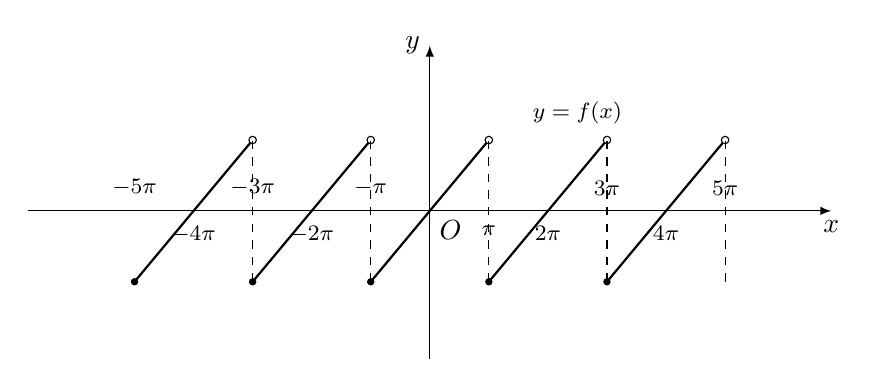
\begin{tikzpicture}[>=latex, scale=0.75]
  \draw[->] (-6.8, 0) -- (6.8, 0) node[below] {$x$};
  \draw[->] (0, -2.5) -- (0, 2.8) node[left] {$y$};
  \node[below right] at (0, 0) {$O$};
  
  \foreach \k in {-2, -1, 0, 1, 2} {
    \draw[thick] (2*\k-1, -1.2) -- (2*\k+1, 1.2);
    \fill (2*\k-1, -1.2) circle (1.8pt);
    \filldraw[fill=white, draw=black] (2*\k+1, 1.2) circle (1.8pt);
    \draw[dashed] (2*\k+1, -1.2) -- (2*\k+1, 1.2);
  }
  
  \draw (-5, 0) node[above=2pt] {\footnotesize $-5\pi$};
  \draw (-4, 0) node[below=2pt] {\footnotesize $-4\pi$};
  \draw (-3, 0) node[above=2pt] {\footnotesize $-3\pi$};
  \draw (-2, 0) node[below=2pt] {\footnotesize $-2\pi$};
  \draw (-1, 0) node[above=2pt] {\footnotesize $-\pi$};
  \draw (1, 0) node[below=2pt] {\footnotesize $\pi$};
  \draw (2, 0) node[below=2pt] {\footnotesize $2\pi$};
  \draw (3, 0) node[above=2pt] {\footnotesize $3\pi$};
  \draw (4, 0) node[below=2pt] {\footnotesize $4\pi$};
  \draw (5, 0) node[above=2pt] {\footnotesize $5\pi$};
  
  \node[above] at (2.5, 1.3) {\footnotesize $y=f(x)$};
\end{tikzpicture}
\caption{}\label{fig:16.1.1}
\end{figure}

\begin{solution}
因为 $x\cos nx$ 与 $x\sin nx$ 分别为奇函数与偶函数, 所以
\[
  a_{n}=\frac{1}{\pi}\int_{-\pi}^{\pi}x\cos nx\,\mathrm{d}x=0,\quad n=0,1,2,\cdots,
\]
\[
  \begin{aligned}
    b_{n}&=\frac{1}{\pi}\int_{-\pi}^{\pi}x\sin nx\,\mathrm{d}x=\frac{2}{\pi}\int_{0}^{\pi}x\sin nx\,\mathrm{d}x=-\frac{2}{n\pi}\int_{0}^{\pi}x\,\mathrm{d}(\cos nx)\\
    &=-\frac{2}{n\pi}\left(\left.x\cos nx\right|_{0}^{\pi}-\int_{0}^{\pi}\cos nx\,\mathrm{d}x\right)=-\frac{2}{n\pi}[\pi(-1)^{n}-0]=(-1)^{n-1}\frac{2}{n},\quad n=1,2,\cdots.
  \end{aligned}
\]
所以,
\[
  f(x)\sim\sum_{n=1}^{\infty}(-1)^{n-1}\frac{2}{n}\sin nx.
\]
根据推论~\ref{cor:16.1.2}, 有
\[
  x=f(x)=\sum_{n=1}^{\infty}(-1)^{n-1}\frac{2}{n}\sin nx,\quad x\in(-\pi,\pi).
\]
进而, 有 (图~\ref{fig:16.1.2})
\[
  \begin{aligned}
    \tilde{f}(x)&=\begin{cases}
      f(x), & x\neq 2k\pi+\pi,\\
      \displaystyle\frac{f(\pi+0)+f(\pi-0)}{2}, & x=2k\pi+\pi,
\end{cases}\quad k=0,\pm 1,\pm 2,\cdots\\
    &=\begin{cases}
      f(x), & x\neq 2k\pi+\pi,\\
      \displaystyle\frac{-\pi+\pi}{2}, & x=2k\pi+\pi,
\end{cases}\quad k=0,\pm 1,\pm 2,\cdots\\
    &=\begin{cases}
      f(x), & x\neq 2k\pi+\pi,\\
      0, & x=2k\pi+\pi,
\end{cases}\quad k=0,\pm 1,\pm 2,\cdots\\
    &=\sum_{n=1}^{\infty}(-1)^{n-1}\frac{2}{n}\sin nx,\quad x\in(-\infty,+\infty).
  \end{aligned}
\]

\begin{figure}[htbp]
\centering
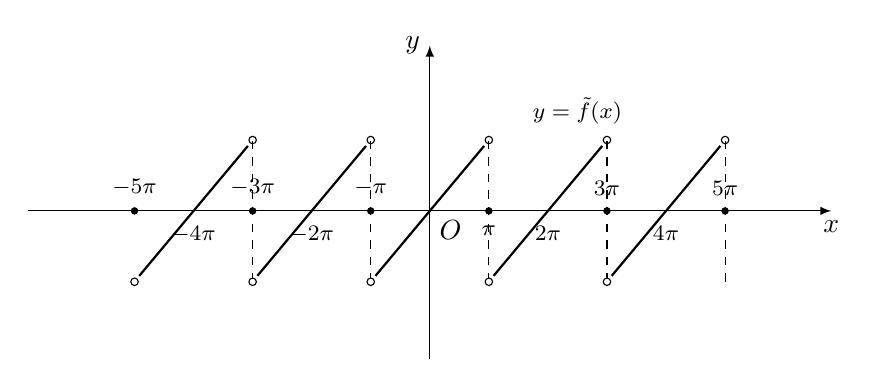
\begin{tikzpicture}[>=latex, scale=0.75]
  \draw[->] (-6.8, 0) -- (6.8, 0) node[below] {$x$};
  \draw[->] (0, -2.5) -- (0, 2.8) node[left] {$y$};
  \node[below right] at (0, 0) {$O$};
  
  \foreach \k in {-2, -1, 0, 1, 2} {
    \draw[thick] (2*\k-0.92, -1.1) -- (2*\k+0.92, 1.1);
    \filldraw[fill=white, draw=black] (2*\k-1, -1.2) circle (1.8pt);
    \filldraw[fill=white, draw=black] (2*\k+1, 1.2) circle (1.8pt);
    \fill (2*\k+1, 0) circle (1.8pt);
    \draw[dashed] (2*\k+1, -1.2) -- (2*\k+1, 1.2);
  }
  \fill (-5, 0) circle (1.8pt);
  
  \draw (-5, 0) node[above=2pt] {\footnotesize $-5\pi$};
  \draw (-4, 0) node[below=2pt] {\footnotesize $-4\pi$};
  \draw (-3, 0) node[above=2pt] {\footnotesize $-3\pi$};
  \draw (-2, 0) node[below=2pt] {\footnotesize $-2\pi$};
  \draw (-1, 0) node[above=2pt] {\footnotesize $-\pi$};
  \draw (1, 0) node[below=2pt] {\footnotesize $\pi$};
  \draw (2, 0) node[below=2pt] {\footnotesize $2\pi$};
  \draw (3, 0) node[above=2pt] {\footnotesize $3\pi$};
  \draw (4, 0) node[below=2pt] {\footnotesize $4\pi$};
  \draw (5, 0) node[above=2pt] {\footnotesize $5\pi$};
  
  \node[above] at (2.5, 1.3) {\footnotesize $y=\tilde{f}(x)$};
\end{tikzpicture}
\caption{}\label{fig:16.1.2}
\end{figure}

取 $x=\displaystyle\frac{\pi}{2}$ 就得到
\[
  \frac{\pi}{2}=\sum_{n=1}^{\infty}(-1)^{n-1}\frac{2}{n}\sin\frac{n\pi}{2},
\]
\[
  \begin{aligned}
    \frac{\pi}{4}&=\sum_{n=1}^{\infty}(-1)^{n-1}\frac{\sin\frac{n\pi}{2}}{n}=\sum_{k=1}^{\infty}(-1)^{2k-2}\frac{\sin\frac{2k-1\pi}{2}}{2k-1}\\
    &=\sum_{k=1}^{\infty}\frac{(-1)^{k-1}}{2k-1}=1-\frac{1}{3}+\frac{1}{5}-\frac{1}{7}+\cdots.
  \end{aligned}
\]
\end{solution}

\begin{example}\label{ex:16.1.2}
设 $f(x)$ 是周期为 $2\pi$ 的函数, 且
\[
  f(x)=\begin{cases}
    x, & x\in(0,2\pi],\\
    2\pi, & x=0.
\end{cases}
\]
求 $f(x)$ 的 Fourier 级数 (图~\ref{fig:16.1.3}) 及函数项级数 $\displaystyle\sum_{n=1}^{\infty}\frac{\sin 2nx}{2n}$, $\displaystyle\sum_{n=1}^{\infty}\frac{\sin 2(n-1)x}{2n-1}$.
\end{example}

\begin{figure}[htbp]
\centering
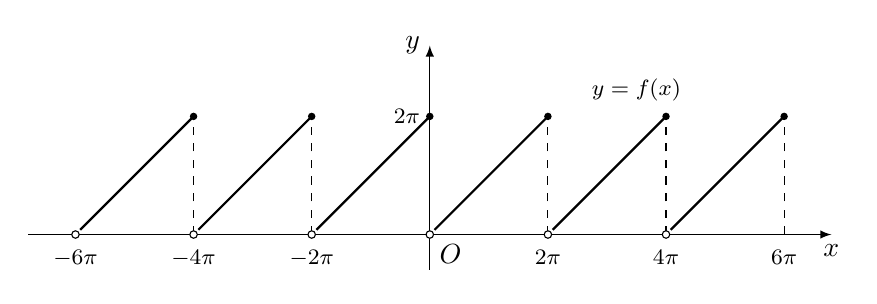
\begin{tikzpicture}[>=latex, scale=0.75]
  \draw[->] (-6.8, 0) -- (6.8, 0) node[below] {$x$};
  \draw[->] (0, -0.6) -- (0, 3.2) node[left] {$y$};
  \node[below right] at (0, 0) {$O$};
  \draw (0, 2) node[left] {\footnotesize $2\pi$};
  
  \foreach \k in {-3, -2, -1, 0, 1, 2} {
    \draw[thick] (2*\k+0.08, 0.08) -- (2*\k+2, 2);
    \filldraw[fill=white, draw=black] (2*\k, 0) circle (1.8pt);
    \fill (2*\k+2, 2) circle (1.8pt);
    \draw[dashed] (2*\k+2, 0) -- (2*\k+2, 2);
  }
  
  \draw (-6, 0) node[below=2pt] {\footnotesize $-6\pi$};
  \draw (-4, 0) node[below=2pt] {\footnotesize $-4\pi$};
  \draw (-2, 0) node[below=2pt] {\footnotesize $-2\pi$};
  \draw (2, 0) node[below=2pt] {\footnotesize $2\pi$};
  \draw (4, 0) node[below=2pt] {\footnotesize $4\pi$};
  \draw (6, 0) node[below=2pt] {\footnotesize $6\pi$};
  
  \node[above] at (3.5, 2.1) {\footnotesize $y=f(x)$};
\end{tikzpicture}
\caption{}\label{fig:16.1.3}
\end{figure}

\begin{solution}
因为
\[
  a_{0}=\frac{1}{\pi}\int_{-\pi}^{\pi}f(x)\,\mathrm{d}x=\frac{1}{\pi}\int_{0}^{2\pi}f(x)\,\mathrm{d}x=\frac{1}{\pi}\int_{0}^{2\pi}x\,\mathrm{d}x=\left.\frac{1}{\pi}\frac{x^{2}}{2}\right|_{0}^{2\pi}=2\pi,
\]
\[
  \begin{aligned}
    a_{n}&=\frac{1}{\pi}\int_{-\pi}^{\pi}f(x)\cos nx\,\mathrm{d}x=\frac{1}{\pi}\int_{0}^{2\pi}f(x)\cos nx\,\mathrm{d}x=\frac{1}{\pi}\int_{0}^{2\pi}x\cos nx\,\mathrm{d}x\\
    &=\frac{1}{n\pi}\int_{0}^{2\pi}x\,\mathrm{d}\sin nx=\frac{1}{n\pi}\left(\left.x\sin nx\right|_{0}^{2\pi}-\int_{0}^{2\pi}\sin nx\,\mathrm{d}x\right)=0,\quad n=1,2,\cdots,
  \end{aligned}
\]
\[
  \begin{aligned}
    b_{n}&=\frac{1}{\pi}\int_{-\pi}^{\pi}f(x)\sin nx\,\mathrm{d}x=\frac{1}{\pi}\int_{0}^{2\pi}f(x)\sin nx\,\mathrm{d}x=\frac{1}{\pi}\int_{0}^{2\pi}x\,\mathrm{d}\left[\frac{\cos nx}{-n}\right]\\
    &=-\frac{1}{n\pi}\left(\left.x\cos nx\right|_{0}^{2\pi}-\int_{0}^{2\pi}\cos nx\,\mathrm{d}x\right)=-\frac{1}{n\pi}(2\pi-0)=-\frac{2}{n},\quad n=1,2,\cdots,
  \end{aligned}
\]
所以,
\[
  f(x)\sim\pi-\sum_{n=1}^{\infty}\frac{2}{n}\sin nx.
\]
根据推论~\ref{cor:16.1.2}, 有
\[
  x=f(x)=\pi-\sum_{n=1}^{\infty}\frac{2}{n}\sin nx,\quad x\in(0,2\pi),
\]
或者
\[
  \frac{\pi-x}{2}=\sum_{n=1}^{\infty}\frac{\sin nx}{n},\quad x\in(0,2\pi).
\]
这正是当年 Abel 给出的例子, 用以说明连续函数项级数的和可能不连续, 根据推论~\ref{cor:13.2.1p}, $\displaystyle\sum_{n=1}^{\infty}\frac{\sin nx}{n}$ 在 $[0,2\pi]$ 上不一致收敛.

进而, 有 (图~\ref{fig:16.1.4})
\[
  \begin{aligned}
    \tilde{f}(x)&=\begin{cases}
      f(x), & x\neq 2k\pi,\\
      \displaystyle\frac{f(0+0)+f(0-0)}{2}, & x=2k\pi,
\end{cases}\quad k=0,\pm 1,\pm 2,\cdots\\
    &=\begin{cases}
      f(x), & x\neq 2k\pi,\\
      \displaystyle\frac{0+2\pi}{2}, & x=2k\pi,
\end{cases}\quad k=0,\pm 1,\pm 2,\cdots\\
    &=\begin{cases}
      f(x), & x\neq 2k\pi,\\
      \pi, & x=2k\pi,
\end{cases}\quad k=0,\pm 1,\pm 2,\cdots\\
    &=\pi-\sum_{n=1}^{\infty}\frac{2}{n}\sin nx,\quad x\in(-\infty,+\infty).
  \end{aligned}
\]

\begin{figure}[htbp]
\centering
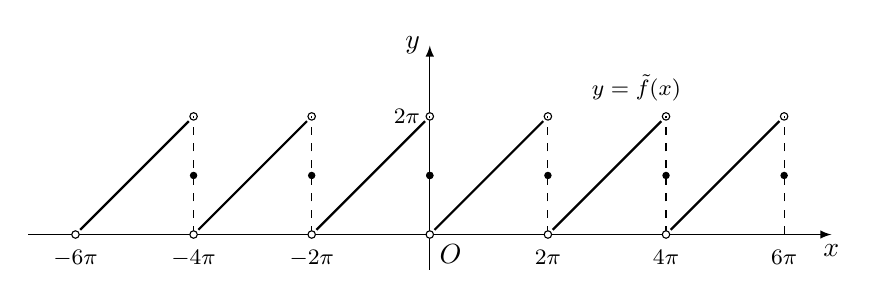
\begin{tikzpicture}[>=latex, scale=0.75]
  \draw[->] (-6.8, 0) -- (6.8, 0) node[below] {$x$};
  \draw[->] (0, -0.6) -- (0, 3.2) node[left] {$y$};
  \node[below right] at (0, 0) {$O$};
  \draw (0, 2) node[left] {\footnotesize $2\pi$};
  
  \foreach \k in {-3, -2, -1, 0, 1, 2} {
    \draw[thick] (2*\k+0.08, 0.08) -- (2*\k+1.92, 1.92);
    \filldraw[fill=white, draw=black] (2*\k, 0) circle (1.8pt);
    \filldraw[fill=white, draw=black] (2*\k+2, 2) circle (1.8pt);
    \fill (2*\k+2, 1) circle (1.8pt);
    \draw[dashed] (2*\k+2, 0) -- (2*\k+2, 2);
  }
  \fill (0, 1) circle (1.8pt);
  
  \draw (-6, 0) node[below=2pt] {\footnotesize $-6\pi$};
  \draw (-4, 0) node[below=2pt] {\footnotesize $-4\pi$};
  \draw (-2, 0) node[below=2pt] {\footnotesize $-2\pi$};
  \draw (2, 0) node[below=2pt] {\footnotesize $2\pi$};
  \draw (4, 0) node[below=2pt] {\footnotesize $4\pi$};
  \draw (6, 0) node[below=2pt] {\footnotesize $6\pi$};
  
  \node[above] at (3.5, 2.1) {\footnotesize $y=\tilde{f}(x)$};
\end{tikzpicture}
\caption{}\label{fig:16.1.4}
\end{figure}

从
\[
  \frac{\pi-x}{2}=\sum_{n=1}^{\infty}\frac{\sin nx}{n},\quad x\in(0,2\pi)
\]
不经计算可得到其他一些有趣的等式. 例如, 将 $x$ 换成 $2x$ 便可得到
\[
  \frac{\pi}{4}-\frac{x}{2}=\sum_{n=1}^{\infty}\frac{\sin 2nx}{2n},\quad x\in(0,\pi).
\]
两式相减就有
\[
  \frac{\pi}{4}=\sum_{n=1}^{\infty}\frac{\sin(2n-1)x}{2n-1},\quad x\in(0,\pi).
\]
令 $x=\displaystyle\frac{\pi}{2}$, 再一次得到
\[
  \frac{\pi}{4}=\sum_{n=1}^{\infty}\frac{\sin(2n-1)\frac{\pi}{2}}{2n-1}=\sum_{n=1}^{\infty}\frac{(-1)^{n-1}}{2n-1}=1-\frac{1}{3}+\frac{1}{5}-\frac{1}{7}+\cdots.
\]
\end{solution}
\begin{example}\label{ex:16.1.3}
将函数 $f(x)=x^{2}$, $x\in[-\pi,\pi]$ 展开为 Fourier 级数. 由此证明:
\[
  \sum_{n=1}^{\infty}\frac{1}{x^{2}}=\frac{\pi^{2}}{6},\quad\sum_{n=1}^{\infty}\frac{(-1)^{n-1}}{n^{2}}=\frac{\pi^{2}}{12}.% 原书如此: 印刷为 x^2, 实为 n^2
\]
\end{example}

\begin{solution}
将 $f(x)$ 的定义延拓到整个数轴上, 使之成为周期为 $2\pi$ 的函数 (图~\ref{fig:16.1.5}), 记延拓后的函数为 $\tilde{f}(x)$, 则 $\tilde{f}(x)$ 是 $(-\infty,+\infty)$ 上的周期为 $2\pi$ 的连续偶函数. 于是,
\[
  a_{0}=\frac{1}{\pi}\int_{-\pi}^{\pi}f(x)\,\mathrm{d}x=\frac{2}{\pi}\int_{0}^{\pi}x^{2}\,\mathrm{d}x=\left.\frac{2}{\pi}\frac{x^{3}}{3}\right|_{0}^{\pi}=\frac{2}{3}\pi^{2},
\]
\[
  \begin{aligned}
    a_{n}&=\frac{1}{\pi}\int_{-\pi}^{\pi}f(x)\cos nx\,\mathrm{d}x=\frac{2}{\pi}\int_{0}^{\pi}x^{2}\cos nx\,\mathrm{d}x=\frac{2}{n\pi}\int_{0}^{\pi}x^{2}\,\mathrm{d}\sin nx\\
    &=\frac{2}{n\pi}\left(\left.x^{2}\sin nx\right|_{0}^{\pi}-\int_{0}^{\pi}2x\sin nx\,\mathrm{d}x\right)=\frac{4}{n^{2}\pi}\int_{0}^{\pi}x\,\mathrm{d}\cos nx\\
    &=\frac{4}{n^{2}\pi}\left(\left.x\cos nx\right|_{0}^{\pi}-\int_{0}^{\pi}cos nx\,\mathrm{d}x\right)=\frac{4}{n^{2}\pi}[\pi(-1)^{n}-0]=(-1)^{n}\frac{4}{n^{2}},\quad n=1,2,\cdots,
  \end{aligned}
\]
\[
  b_{n}=\frac{1}{\pi}\int_{-\pi}^{\pi}f(x)\sin nx\,\mathrm{d}x=\frac{1}{\pi}\int_{-\pi}^{\pi}x^{2}\sin nx\,\mathrm{d}x\xlongequal{\text{奇函数}}0,\quad n=1,2,\cdots.
\]

\begin{figure}[htbp]
\centering
\begin{tikzpicture}[>=latex, scale=0.8]
  \draw[->] (-10.5, 0) -- (10.5, 0) node[below] {$x$};
  \draw[->] (0, -0.6) -- (0, 3.8) node[left] {$y$};
  \node[below right] at (0, 0) {$O$};
  \draw (0, 3.1) node[left] {\footnotesize $\pi^2$};
  
  \foreach \k in {-1, 0, 1} {
    \draw[thick, smooth, domain=-3.14159:3.14159, variable=\t] plot ({2*\k*3.14159/1.8 + \t/1.8}, {(\t)^2 / (3.14159^2) * 3.1});
  }
  
  \draw (-3*3.14159/1.8, 0) node[below=2pt] {\footnotesize $-3\pi$};
  \draw (-2*3.14159/1.8, 0) node[below=2pt] {\footnotesize $-2\pi$};
  \draw (-3.14159/1.8, 0) node[below=2pt] {\footnotesize $-\pi$};
  \draw (3.14159/1.8, 0) node[below=2pt] {\footnotesize $\pi$};
  \draw (2*3.14159/1.8, 0) node[below=2pt] {\footnotesize $2\pi$};
  \draw (3*3.14159/1.8, 0) node[below=2pt] {\footnotesize $3\pi$};
  
  \draw[dashed] (-3*3.14159/1.8, 0) -- (-3*3.14159/1.8, 3.1);
  \draw[dashed] (3*3.14159/1.8, 0) -- (3*3.14159/1.8, 3.1);
  
  \node[above] at (1.8*3.14159/1.8, 3.1) {\footnotesize $y=\tilde{f}(x)$};
\end{tikzpicture}
\caption{}\label{fig:16.1.5}
\end{figure}

根据推论~\ref{cor:16.1.2}, 有
\[
  \tilde{f}(x)=\frac{\pi^{2}}{3}+4\sum_{n=1}^{\infty}\frac{(-1)^{n}}{n^{2}}\cos nx,\quad x\in(-\infty,+\infty).
\]
限制在区间 $[-\pi,\pi]$ 上有
\[
  x^{2}=f(x)=\frac{\pi^{2}}{3}+4\sum_{n=1}^{\infty}\frac{(-1)^{n}}{n^{2}}\cos nx,\quad x\in[-\pi,\pi],
\]
或者
\[
  \sum_{n=1}^{\infty}(-1)^{n}\frac{\cos nx}{n^{2}}=\frac{x^{2}}{4}-\frac{\pi^{2}}{12},\quad x\in[-\pi,\pi].
\]
令 $x=\pi$ 就得
\[
  \sum_{n=1}^{\infty}\frac{1}{n^{2}}=\frac{\pi^{2}}{4}-\frac{\pi^{2}}{12}=\frac{\pi^{2}}{6}.
\]
令 $x=0$ 就得
\[
  \sum_{n=1}^{\infty}\frac{(-1)^{n}}{n^{2}}=\frac{0^{2}}{4}-\frac{\pi^{2}}{12}=-\frac{\pi^{2}}{12},
\]
\[
  \sum_{n=1}^{\infty}\frac{(-1)^{n-1}}{n^{2}}=\frac{\pi^{2}}{12}.
\]
\end{solution}

\begin{example}\label{ex:16.1.4}
设 $a$ 不为整数, 将 $f(x)=\cos ax$ 在 $[-\pi,\pi]$ 上展开为 Fourier 级数并证明
\[
  \frac{\pi}{\sin a\pi}=\frac{1}{a}+\sum_{n=1}^{\infty}(-1)^{n}\frac{2a}{a^{2}-n^{2}},\quad a\notin\mathbb{Z}.
\]
\end{example}

\begin{solution}
将 $f(x)$ 延拓为整个数轴上的以 $2\pi$ 为周期的函数, 记延拓后的函数为 $\tilde{f}(x)$, 则 $\tilde{f}(x)$ 是 $(-\infty,+\infty)$ 上的周期为 $2\pi$ 的连续偶函数. 因此,
\[
  a_{n}=\frac{1}{n}\int_{-\pi}^{\pi}f(x)\cos ax\,\mathrm{d}x=\frac{2}{\pi}\int_{0}^{\pi}\cos ax\cos nx\,\mathrm{d}x% 原书如此: 印刷为 \frac{1}{n} 和 \cos ax
\]
\[
  \begin{aligned}
    &=\frac{1}{\pi}\int_{0}^{\pi}[\cos(a-n)x+\cos(a+n)x]\,\mathrm{d}x=\left.\frac{1}{\pi}\left[\frac{\sin(a-n)x}{a-n}+\frac{\sin(a+n)x}{a+n}\right]\right|_{0}^{\pi}\\
    &=\frac{1}{\pi}\left[\frac{\sin(a-n)\pi}{a-n}+\frac{\sin(a+n)\pi}{a+n}\right]=\frac{1}{\pi}\left[\frac{(-1)^{n}\sin a\pi}{a-n}+\frac{(-1)^{n}\sin a\pi}{a+n}\right]\\
    &=\frac{(-1)^{n}}{\pi}\frac{2a\sin a\pi}{a^{2}-n^{2}},\quad n=0,1,2,\cdots,
  \end{aligned}
\]
\[
  b_{n}=\frac{1}{\pi}\int_{-\pi}^{\pi}f(x)\sin ax\,\mathrm{d}x=\frac{1}{\pi}\int_{-\pi}^{\pi}\cos ax\sin nx\,\mathrm{d}x\xlongequal{\text{奇函数}}0,\quad n=1,2,\cdots.% 原书如此: 前式印刷为 \sin ax
\]
根据推论~\ref{cor:16.1.2}, 可知 $\tilde{f}(x)$ 的 Fourier 级数为
\[
  \tilde{f}(x)=\frac{\sin a\pi}{\pi}\left[\frac{1}{a}+\sum_{n=1}^{\infty}(-1)^{n}\frac{2a}{a^{2}-n^{2}}\cos nx\right],\quad x\in(-\infty,+\infty).
\]
限制在 $[-\pi,\pi]$ 上就有
\[
  \cos ax=\frac{\sin a\pi}{\pi}\left[\frac{1}{a}+\sum_{n=1}^{\infty}(-1)^{n}\frac{2a}{a^{2}-n^{2}}\cos nx\right],\quad x\in[-\pi,\pi].
\]
如果在上式中, 令 $x=0$, 就可得
\[
  \frac{\pi}{\sin a\pi}=\frac{1}{a}+\sum_{n=1}^{\infty}(-1)^{n}\frac{2a}{a^{2}-n^{2}},\quad a\notin\mathbb{Z}.
\]
\end{solution}

应用例~\ref{ex:16.1.4} 中的公式
\[
  \frac{\pi}{\sin a\pi}=\frac{1}{a}+\sum_{n=1}^{\infty}(-1)^{n}\frac{2a}{a^{2}-n^{2}},\quad a\notin\mathbb{Z}
\]
可以计算出下面积分的值.

\begin{example}\label{ex:16.1.5}
证明: 无穷积分
\[
  \int_{0}^{+\infty}\frac{x^{p-1}}{1+x}\,\mathrm{d}x=\frac{1}{p}+\sum_{n=1}^{\infty}(-1)^{n}\frac{2p}{p^{2}-n^{2}}=\frac{\pi}{\sin p\pi},\quad 0<p<1.
\]
\end{example}

\begin{proof}
当 $0<x<1$ 时, 有展开式
\[
  \frac{x^{p-1}}{1+x}=\sum_{n=0}^{\infty}(-1)^{n}x^{n+p-1},
\]
且这个级数在区间 $(0,1)$ 的任何内闭区间 $[a,b]\subset(0,1)$ 上都一致收敛, 如果记它的部分和为 $f_{n}(x)$, 则 $\{f_{n}(x)\}$ 在区间 $(0,1)$ 的任何内闭区间 $[a,b]\subset(0,1)$ 上一致收敛. 由于
\[
  0\leqslant f_{n}(x)=\sum_{k=0}^{n-1}(-1)^{k}x^{k+p-1}=\frac{x^{p-1}[1-(-1)^{n}x^{n}]}{1+x}\leqslant 2\cdot\frac{x^{p-1}}{1+x}\leqslant 2x^{p-1},
\]
而 $\displaystyle\int_{0}^{1}x^{p-1}\,\mathrm{d}x$ 收敛, 故 $\displaystyle\int_{0}^{1}f_{n}(x)\,\mathrm{d}x$ 关于 $n$ 一致收敛.
\[
  \begin{aligned}
    \int_{0}^{1}\frac{x^{p-1}}{1+x}\,\mathrm{d}x&=\int_{0}^{1}\sum_{n=0}^{\infty}(-1)^{n}x^{n+p-1}\,\mathrm{d}x\xlongequal{\text{定理~\ref{thm:15.2.6}}}\sum_{n=0}^{\infty}(-1)^{n}\int_{0}^{1}x^{n+p-1}\,\mathrm{d}x\\
    &=\sum_{n=0}^{\infty}\frac{(-1)^{n}}{n+p}.
  \end{aligned}
\]
进而, 有
\[
  \begin{aligned}
    \int_{1}^{+\infty}\frac{x^{p-1}}{1+x}\,\mathrm{d}x&\xlongequal{x=\frac{1}{t}}\int_{1}^{0}\frac{\left(\frac{1}{t}\right)^{p-1}}{1+\frac{1}{t}}\cdot\frac{-1}{t^{2}}\,\mathrm{d}t=\int_{0}^{1}\frac{t^{-p}}{1+t}\,\mathrm{d}t\\
    &=\int_{0}^{1}\frac{t^{(1-p)+1}}{1+t}\,\mathrm{d}t\xlongequal{\text{由上面结果}}\sum_{n=0}^{\infty}\frac{(-1)^{n}}{n+1-p}=\sum_{n=1}^{\infty}\frac{(-1)^{n}}{p-n}.% 原书如此: 印刷为 t^{(1-p)+1}
  \end{aligned}
\]
综合上述得到
\[
  \begin{aligned}
    \int_{0}^{+\infty}\frac{x^{p-1}}{1+x}\,\mathrm{d}x&=\int_{0}^{1}\frac{x^{p-1}}{1+x}\,\mathrm{d}x+\int_{1}^{+\infty}\frac{x^{p-1}}{1+x}\,\mathrm{d}x\\
    &=\sum_{n=0}^{\infty}\frac{(-1)^{n}}{p+n}+\sum_{n=1}^{\infty}\frac{(-1)^{n}}{p-n}=\frac{1}{p}+\sum_{n=1}^{\infty}(-1)^{n}\frac{2p}{p^{2}-n^{2}}\\
    &\xlongequal{\text{例~\ref{ex:16.1.4}}}\frac{\pi}{\sin p\pi},\quad 0<p<1.
  \end{aligned}
\]
\end{proof}

\begin{example}\label{ex:16.1.6}
将函数 $\mathrm{e}^{ax}$ 在区间 $(0,2\pi)$ 上展开为 Fourier 级数, 并求 $\displaystyle\sum_{n=1}^{\infty}\frac{1}{1+n^{2}}$.
\end{example}

\begin{solution}
先计算 Fourier 系数:
\[
  \begin{aligned}
    a_{n}&=\frac{1}{\pi}\int_{0}^{2\pi}\mathrm{e}^{ax}\cos nx\,\mathrm{d}x=\left.\frac{1}{\pi}\frac{\mathrm{e}^{ax}}{a^{2}+n^{2}}(a\cos nx+n\sin nx)\right|_{0}^{2\pi}\\
    &=\frac{\mathrm{e}^{2\pi a}-1}{\pi}\frac{a}{a^{2}+n^{2}},\quad n=0,1,2,\cdots.
  \end{aligned}
\]
\[
  \begin{aligned}
    b_{n}&=\frac{1}{\pi}\int_{0}^{2\pi}\mathrm{e}^{ax}\sin nx\,\mathrm{d}x=\left.\frac{1}{\pi}\frac{\mathrm{e}^{ax}}{a^{2}+n^{2}}(a\sin nx-n\cos nx)\right|_{0}^{2\pi}\\
    &=\frac{\mathrm{e}^{2\pi a}-1}{\pi}\frac{-n}{a^{2}+n^{2}},\quad n=1,2,\cdots.
  \end{aligned}
\]
于是,
\[
  \mathrm{e}^{ax}=\frac{\mathrm{e}^{2\pi a}-1}{\pi}\left(\frac{1}{2a}+\sum_{n=1}^{\infty}\frac{a\cos nx-n\sin nx}{a^{2}+n^{2}}\right),\quad 0<x<2\pi.
\]
如果将 $f(x)=\mathrm{e}^{ax}$ ($0<x<2\pi$) 延拓为 $(-\infty,+\infty)$ 上以 $2\pi$ 为周期的函数 $\tilde{f}(x)$, 则必须有
\[
  \tilde{f}(0)=\tilde{f}(2\pi)=\frac{f(2\pi-0)+f(0+0)}{2}=\frac{\mathrm{e}^{2\pi a}+\mathrm{e}^{0\cdot a}}{2}=\frac{\mathrm{e}^{2\pi a}+1}{2}.
\]
由此得到
\[
  \tilde{f}(x)=\frac{\mathrm{e}^{2\pi a}-1}{\pi}\left(\frac{1}{2a}+\sum_{n=1}^{\infty}\frac{a\cos nx-n\sin nx}{a^{2}+n^{2}}\right),\quad -\infty<x<+\infty.
\]
令 $a=1$, $x=0$, 就有
\[
  \frac{\mathrm{e}^{2\pi}+1}{2}=\frac{\mathrm{e}^{2\pi}-1}{\pi}\left(\frac{1}{2}+\sum_{n=1}^{\infty}\frac{1}{1+n^{2}}\right),
\]
即
\[
  \sum_{n=1}^{\infty}\frac{1}{1+n^{2}}=\frac{\mathrm{e}^{2\pi}+1}{2}\cdot\frac{\pi}{\mathrm{e}^{2\pi}-1}-\frac{1}{2}=\frac{\pi}{2}\frac{\mathrm{e}^{2\pi}+1}{\mathrm{e}^{2\pi}-1}-\frac{1}{2}.
\]
\end{solution}

\begin{remark}\label{rem:16.1.2}
从例~\ref{ex:16.1.1}$\sim$例~\ref{ex:16.1.4}, 例~\ref{ex:16.1.6} 可看到, 经某个函数的 Fourier 级数的计算, 并取特殊点求得一些数项级数之和, 这些数项级数之和是难以用其他方法得到的.
\end{remark}

上面各例都是先给出函数在 $(-\pi,\pi)$ 或 $(0,2\pi)$ 上的表达式, 然后将它延拓为整个数轴上的周期 $2\pi$ 的函数, 再将它展开为 Fourier 级数.

对于只在 $(0,\pi)$ 上定义的函数, 如何展开为 Fourier 级数呢? 这时, 在 $(-\pi,0)$ 上可以任意补充 $f(x)$ 的定义, 使 $f(x)$ 在 $(-\pi,\pi)$ 上有定义, 然后再将它以 $2\pi$ 为周期延拓到整个数轴上去. 对于各种不同的延拓, 得到的 Fourier 级数自然也是不同的. 但在 $(0,\pi)$ 上, 它们都收敛到同一个函数. 而偶性延拓与奇性延拓是常用的两种延拓方法.

\begin{definition}\label{def:16.1.3}
设 $f(x)$ 是定义在 $(0,\pi)$ 上的函数, 令
\[
  f(x)=f(-x),\quad x\in(-\pi,0)
\]
来补充 $f(x)$ 在 $(-\pi,0)$ 上的定义, 使 $f(x)$ 在 $(-\pi,\pi)$ 上成为偶函数 (延拓后的函数 $\tilde{f}(x)$ 仍记为 $f(x)$), 这种延拓方法称为\textbf{偶性延拓}. 这样便有
\[
  a_{n}=\frac{1}{\pi}\int_{-\pi}^{\pi}f(x)\cos nx\,\mathrm{d}x=\frac{2}{\pi}\int_{0}^{\pi}f(x)\cos nx\,\mathrm{d}x,\quad n=0,1,2,\cdots,
\]
\[
  b_{n}=\frac{1}{\pi}\int_{-\pi}^{\pi}f(x)\sin nx\,\mathrm{d}x=0,\quad n=1,2,\cdots.
\]
因此, $f(x)$ 的 Fourier 级数中只含余弦项:
\[
  f(x)\sim\frac{a_{0}}{2}+\sum_{n=1}^{\infty}a_{n}\cos nx,
\]
称它为 $f(x)$, $x\in(0,\pi)$ 的\textbf{余弦级数}.

如果令
\[
  f(x)=-f(-x),\quad x\in(-\pi,0)
\]
来补充 $f(x)$ 在 $(-\pi,0)$ 上的定义, 使 $f(x)$ 在 $(-\pi,\pi)$ 上成为奇函数 (延拓后的函数 $\tilde{f}(x)$ 仍记为 $f(x)$), 这种延拓方法称为\textbf{奇性延拓} (注意: 由 $f(0)=f(-0)=-f(0)$, 知 $f(0)=0$). 这样便有
\[
  a_{n}=\frac{1}{\pi}\int_{-\pi}^{\pi}f(x)\cos nx\,\mathrm{d}x=0,\quad n=0,1,2,\cdots,
\]
\[
  b_{n}=\frac{1}{\pi}\int_{-\pi}^{\pi}f(x)\sin nx\,\mathrm{d}x=\frac{2}{\pi}\int_{0}^{\pi}f(x)\sin nx\,\mathrm{d}x,\quad n=1,2,\cdots.
\]
因此, $f(x)$ 的 Fourier 级数中只含正弦项:
\[
  f(x)\sim\sum_{n=1}^{\infty}b_{n}\sin nx,
\]
称它为 $f(x)$, $x\in(0,\pi)$ 的\textbf{正弦级数}.
\end{definition}

由此可见, 对于只定义在区间 $(0,\pi)$ 上的函数, 只要满足 Dini 定理的条件, 就可考虑它的正弦级数, 也可考虑它的余弦级数.

\begin{example}\label{ex:16.1.7}
将函数
\[
  f(x)=x,\quad x\in(0,\pi)
\]
分别展开为余弦级数与正弦级数.
\end{example}

\begin{solution}
若要展开成余弦级数, 可先将 $f(x)$, $x\in(0,\pi)$ 偶性延拓到区间 $(-\pi,0)$ 上, 然后再将它以周期 $2\pi$ 延拓到整个区间 $(-\infty,+\infty)$ 上, 所得的函数记为 $\tilde{f}(x)$ (图~\ref{fig:16.1.6}). 于是,
\[
  a_{0}=\frac{2}{\pi}\int_{0}^{\pi}x\,\mathrm{d}x=\pi,
\]
\[
  \begin{aligned}
    a_{n}&=\frac{2}{\pi}\int_{0}^{\pi}x\cos nx\,\mathrm{d}x=\frac{2}{n\pi}\int_{0}^{\pi}x\,\mathrm{d}\sin nx\\
    &=\frac{2}{n\pi}\left(\left.x\sin nx\right|_{0}^{\pi}-\int_{0}^{\pi}\sin nx\,\mathrm{d}x\right)=\left.\frac{2}{n^{2}\pi}\cos nx\right|_{0}^{\pi}\\
    &=\frac{2}{n^{2}\pi}[(-1)^{n}-1]=\begin{cases}
      0, & n=2k,\\
      \displaystyle-\frac{4}{(2k-1)^{2}\pi}, & n=2k-1,
\end{cases}\quad k=1,2,\cdots,
  \end{aligned}
\]
\[
  b_{n}=0,\quad n=1,2,\cdots.
\]
所以,
\[
  x=\frac{\pi}{2}-\frac{4}{\pi}\sum_{k=1}^{\infty}\frac{\cos(2k-1)x}{(2k-1)^{2}},\quad x\in[0,\pi].% 原书如此: 公式中分子印刷为 \cos(2k-1)\pi
\]
\[
  \tilde{f}(x)=\frac{\pi}{2}-\frac{4}{\pi}\sum_{k=1}^{\infty}\frac{\cos(2k-1)x}{(2k-1)^{2}},\quad x\in(-\infty,+\infty).% 原书如此: 同样印刷为 \cos(2k-1)\pi
\]

\begin{figure}[htbp]
\centering
\begin{tikzpicture}[>=latex, scale=0.85]
  \draw[->] (-7.5, 0) -- (7.5, 0) node[below] {$x$};
  \draw[->] (0, -0.6) -- (0, 3.2) node[left] {$y$};
  \node[below right] at (0, 0) {$O$};
  
  % 刻度标记
  \draw (-2*2.2, 0) node[below=2pt] {\footnotesize $-2\pi$};
  \draw (-2.2, 0) node[below=2pt] {\footnotesize $-\pi$};
  \draw (2.2, 0) node[below=2pt] {\footnotesize $\pi$};
  \draw (2*2.2, 0) node[below=2pt] {\footnotesize $2\pi$};
  
  % 折线段
  \draw[thick] (-2*2.2, 0) -- (-2.2, 2.2);
  \draw[thick, dashed] (-2.2, 2.2) -- (0, 0);
  \draw[thick] (0, 0) -- (2.2, 2.2) -- (2*2.2, 0);
  \draw[thick] (-2*2.2, 0) -- (-2.6*2.2, 0.6*2.2);
  \draw[thick] (2*2.2, 0) -- (2.6*2.2, 0.6*2.2);
\end{tikzpicture}
\caption{}\label{fig:16.1.6}
\end{figure}

令 $x=0$ 得
\[
  \sum_{k=1}^{\infty}\frac{1}{(2k-1)^{2}}=\frac{\pi^{2}}{8}.
\]
此数项级数之和也可如下得到:
\[
  \sum_{n=1}^{\infty}\frac{1}{n^{2}}=\sum_{k=1}^{\infty}\frac{1}{(2k-1)^{2}}+\sum_{k=1}^{\infty}\frac{1}{(2k)^{2}},
\]
\[
  \sum_{k=1}^{\infty}\frac{1}{(2k-1)^{2}}=\sum_{n=1}^{\infty}\frac{1}{n^{2}}-\sum_{k=1}^{\infty}\frac{1}{(2k)^{2}}=\frac{3}{4}\sum_{n=1}^{\infty}\frac{1}{n^{2}}\xlongequal{\text{例~\ref{ex:16.1.3}}}\frac{3}{4}\times\frac{\pi^{2}}{6}=\frac{\pi^{2}}{8}.
\]
若要展开成正弦级数, 可先将 $f(x)$, $x\in(0,\pi)$ 奇性延拓到 $(-\pi,0)$ 上, 然后再将它以周期 $2\pi$ 延拓到整个区间 $(-\infty,+\infty)$ 上, 所得的函数记为 $\tilde{f}(x)$ (图~\ref{fig:16.1.7}). 于是, 由例~\ref{ex:16.1.1} 知
\[
  x=2\sum_{n=1}^{\infty}(-1)^{n-1}\frac{\sin nx}{n},\quad x\in[0,\pi).
\]

\begin{figure}[htbp]
\centering
\begin{tikzpicture}[>=latex, scale=0.85]
  \draw[->] (-8.5, 0) -- (8.5, 0) node[below] {$x$};
  \draw[->] (0, -2.6) -- (0, 2.8) node[left] {$y$};
  \node[below right] at (0, 0) {$O$};
  
  % 刻度标记
  \draw (-3*2.2, 0) node[below=2pt] {\footnotesize $-3\pi$};
  \draw (-2*2.2, 0) node[below=2pt] {\footnotesize $-2\pi$};
  \draw (-2.2, 0) node[below=2pt] {\footnotesize $-\pi$};
  \draw (2.2, 0) node[below=2pt] {\footnotesize $\pi$};
  \draw (2*2.2, 0) node[below=2pt] {\footnotesize $2\pi$};
  \draw (3*2.2, 0) node[below=2pt] {\footnotesize $3\pi$};
  
  % 中间周期
  \draw[thick, dashed] (-2.2+0.05, -1.8+0.05) -- (0, 0);
  \draw[thick] (0, 0) -- (2.2-0.05, 1.8-0.05);
  \filldraw[fill=white, draw=black] (-2.2, -1.8) circle (1.8pt);
  \filldraw[fill=white, draw=black] (2.2, 1.8) circle (1.8pt);
  
  % 右侧周期
  \draw[thick] (2.2+0.05, -1.8+0.05) -- (3*2.2-0.05, 1.8-0.05);
  \filldraw[fill=white, draw=black] (2.2, -1.8) circle (1.8pt);
  \filldraw[fill=white, draw=black] (3*2.2, 1.8) circle (1.8pt);
  
  % 左侧周期
  \draw[thick] (-3*2.2+0.05, -1.8+0.05) -- (-2.2-0.05, 1.8-0.05);
  \filldraw[fill=white, draw=black] (-3*2.2, -1.8) circle (1.8pt);
  \filldraw[fill=white, draw=black] (-2.2, 1.8) circle (1.8pt);
\end{tikzpicture}
\caption{}\label{fig:16.1.7}
\end{figure}

如果 $\tilde{f}[(2k-1)\pi]=\frac{\pi+(-\pi)}{2}=0$, 则
\[
  \tilde{f}(x)=2\sum_{n=1}^{\infty}(-1)^{n-1}\frac{\sin nx}{n},\quad x\in(-\infty,+\infty).
\]
\end{solution}

下面来讨论周期为 $2l$ 的函数的 Fourier 展开.

\begin{definition}\label{def:16.1.4}
设 $f(x)$ 是以 $2l$ 为周期的函数, 作变换 $x=\frac{l}{\pi}t$, 并记
\[
  f(x)=f\left(\frac{l}{\pi}t\right)=g(t),
\]
则 $g(t)$ 是周期为 $2\pi$ 的函数. 如果 $g(t)$ 满足 Dini 定理推论的条件, 便有
\[
  g(t)=\frac{a_{0}}{2}+\sum_{n=1}^{\infty}(a_{n}\cos nt+b_{n}\sin nt),\quad t\in(-\infty,+\infty),
\]
其中
\[
  a_{n}=\frac{1}{\pi}\int_{-\pi}^{\pi}g(t)\cos nt\,\mathrm{d}t,\quad n=0,1,2,\cdots,
\]
\[
  b_{n}=\frac{1}{\pi}\int_{-\pi}^{\pi}g(t)\sin nt\,\mathrm{d}t,\quad n=1,2,\cdots.
\]
回到原来的变量 $x$ 就有
\[
  f(x)=\frac{a_{0}}{2}+\sum_{n=1}^{\infty}\left(a_{n}\cos\frac{n\pi}{l}x+b_{n}\sin\frac{n\pi}{l}x\right),\quad x\in(-\infty,+\infty),
\]
而
\[
  \begin{aligned}
    a_{n}&=\frac{1}{\pi}\int_{-\pi}^{\pi}g(t)\cos nt\,\mathrm{d}t\xlongequal{t=\frac{\pi}{l}x}\frac{1}{\pi}\int_{-l}^{l}f(x)\cos\frac{n\pi}{l}x\,\mathrm{d}\left(\frac{\pi}{l}x\right)\\
    &=\frac{1}{l}\int_{-l}^{l}f(x)\cos\frac{n\pi}{l}x\,\mathrm{d}x,\quad n=0,1,2,\cdots,
  \end{aligned}
\]
\[
  \begin{aligned}
    b_{n}&=\frac{1}{\pi}\int_{-\pi}^{\pi}g(t)\sin nt\,\mathrm{d}t\xlongequal{t=\frac{\pi}{l}x}\frac{1}{\pi}\int_{-l}^{l}f(x)\sin\frac{n\pi}{l}x\,\mathrm{d}\left(\frac{\pi}{l}x\right)\\
    &= \frac{1}{l}\int_{-l}^{l}f(x)\sin\frac{n\pi}{l}x\,\mathrm{d}x,\quad n=1,2,\cdots.
  \end{aligned}
\]
这就给出了周期 $2l$ 的函数 $f(x)$ 的 Fourier 展开式.

如果 $f(x)$ 只定义在 $(0,l)$ 上, 则它既可展开为余弦级数
\[
  f(x)=\frac{a_{0}}{2}+\sum_{n=1}^{\infty}a_{n}\cos\frac{n\pi}{l}x,
\]
其中
\[
  a_{n}=\frac{2}{l}\int_{0}^{l}f(x)\cos\frac{n\pi}{l}x\,\mathrm{d}x,\quad n=0,1,2,\cdots,
\]
也可展开为正弦级数
\[
  f(x)=\sum_{n=1}^{\infty}b_{n}\sin\frac{n\pi}{l}x,
\]
其中
\[
  b_{n}=\frac{2}{l}\int_{0}^{l}f(x)\sin\frac{n\pi}{l}x\,\mathrm{d}x,\quad n=1,2,\cdots.
\]
\end{definition}

\begin{example}\label{ex:16.1.8}
将函数
\[
  f(x)=\begin{cases}
    x, & x\in\left[0,\dfrac{l}{2}\right],\\
    l-x, & x\in\left[\dfrac{l}{2},l\right]
\end{cases}
\]
在 $[0,l]$ 上展开为正弦级数.
\end{example}

\begin{solution}
将 $f(x)$ 作奇性延拓 (图~\ref{fig:16.1.8}) 得 $\tilde{f}(x)$, 则
\[
  \begin{aligned}
    b_{n}&=\frac{2}{l}\int_{0}^{l}f(x)\sin\frac{n\pi}{l}x\,\mathrm{d}x\\
    &=\frac{2}{l}\int_{0}^{\frac{l}{2}}x\sin\frac{n\pi}{l}x\,\mathrm{d}x+\frac{2}{l}\int_{\frac{l}{2}}^{l}(l-x)\sin\frac{n\pi}{l}x\,\mathrm{d}x\\
    &=\frac{2}{l}\int_{0}^{\frac{l}{2}}x\,\mathrm{d}\left(-\frac{l}{n\pi}\cos\frac{n\pi}{l}x\right)+\frac{2}{l}\int_{\frac{l}{2}}^{l}(l-x)\,\mathrm{d}\left(-\frac{l}{n\pi}\cos\frac{n\pi}{l}x\right)\\
    &=\frac{2}{l}\left(-\left.\frac{l}{n\pi}x\cos\frac{n\pi}{l}x\right|_{0}^{\frac{l}{2}}+\int_{0}^{\frac{l}{2}}\frac{l}{n\pi}\cos\frac{n\pi}{l}x\,\mathrm{d}x\right.\\
    &\quad\left.-\left.\frac{l}{n\pi}(l-x)\cos\frac{n\pi}{l}x\right|_{\frac{l}{2}}^{l}-\frac{l}{n\pi}\int_{\frac{l}{2}}^{l}\cos\frac{n\pi}{l}x\,\mathrm{d}x\right)\\
    &=\frac{2}{n\pi}\left(-\frac{l}{2}\cos\frac{n\pi}{2}+\left.\frac{l}{n\pi}\sin\frac{n\pi}{l}x\right|_{0}^{\frac{l}{2}}+\frac{l}{2}\cos\frac{n\pi}{2}-\left.\frac{l}{n\pi}\sin\frac{n\pi}{l}x\right|_{\frac{l}{2}}^{l}\right)\\
    &=\frac{2}{n\pi}\left(\frac{l}{n\pi}\sin\frac{n\pi}{2}+\frac{l}{n\pi}\sin\frac{n\pi}{2}\right)=\frac{4l}{n^{2}\pi^{2}}\sin\frac{n\pi}{2}\\
    &=\begin{cases}
      0, & n=2k,\\
      \displaystyle\frac{4l}{\pi^{2}}\frac{(-1)^{k}}{(2k+1)^{2}}, & n=2k+1,
\end{cases}\quad k=0,1,2,\cdots.
  \end{aligned}
\]
由此得到 $f(x)$, $x\in[0,l]$ 的正弦展开式为
\[
  f(x)=\frac{4l}{\pi^{2}}\sum_{k=0}^{\infty}\frac{(-1)^{k}}{(2k+1)^{2}}\sin\frac{2k+1}{l}\pi x,\quad x\in[0,l].% 原书如此: 印刷为 x\in[0,1]
\]
\[
  \tilde{f}(x)=\frac{4l}{\pi^{2}}\sum_{k=0}^{\infty}\frac{(-1)^{k}}{(2k+1)^{2}}\sin\frac{2k+1}{l}\pi x,\quad x\in(-\infty,+\infty).
\]
\end{solution}

\begin{center}
\begin{minipage}{\linewidth}
\centering
\begin{tikzpicture}[>=latex, scale=0.75]
  \draw[->] (-5, 0) -- (5, 0) node[below] {$x$};
  \draw[->] (0, -2.2) -- (0, 2.4) node[left] {$y$};
  \node[below right] at (0, 0) {$O$};
  
  \coordinate (L2) at (1.6, 0);
  \coordinate (L) at (3.2, 0);
  \coordinate (NL2) at (-1.6, 0);
  \coordinate (NL) at (-3.2, 0);
  \coordinate (TOP) at (1.6, 1.6);
  \coordinate (BOT) at (-1.6, -1.6);
  
  % 实线部分 (正侧)
  \draw[thick] (0, 0) -- (TOP) -- (L);
  % 虚线部分 (负侧奇延拓)
  \draw[thick, dashed] (NL) -- (BOT) -- (0, 0);
  
  % 辅助线
  \draw[dashed] (0, 1.6) node[left] {\footnotesize $\dfrac{l}{2}$} -- (TOP) -- (1.6, 0);
  \draw[dashed] (0, -1.6) node[right=1pt] {\footnotesize $-\dfrac{l}{2}$} -- (BOT) -- (-1.6, 0);
  
  % 坐标标注
  \draw (1.6, 0) node[below=2pt] {\footnotesize $\dfrac{l}{2}$};
  \draw (3.2, 0) node[below=2pt] {\footnotesize $l$};
  \draw (-1.6, 0) node[above=2pt] {\footnotesize $-\dfrac{l}{2}$};
  \draw (-3.2, 0) node[below=2pt] {\footnotesize $-l$};
  
  \node[above] at (1.5, 0.9) {\footnotesize $f(x)$};
\end{tikzpicture}
\captionof{figure}{}\label{fig:16.1.8}
\end{minipage}
\end{center}

\begin{exblock}{练习题 16.1}
\item 证明: 三角多项式
\[
  T_{n}(x)=\sum_{k=0}^{n}(\alpha_{k}\cos kx+\beta_{k}\sin kx)
\]
的 Fourier 级数就是它本身.
\item 设 $f(x)$ 是周期为 $2\pi$ 的可积或绝对可积函数. 证明:

(1) 如果 $f(x)$ 在 $[-\pi,\pi]$ 中满足 $f(x+\pi)=f(x)$, 则 $a_{2n-1}=b_{2n-1}=0$, $n=1,2,\cdots$;

(2) 如果 $f(x)$ 在 $[-\pi,\pi]$ 中满足 $f(x+\pi)=-f(x)$, 则 $a_{2n}=b_{2n}=0$, $n=0,1,2,\cdots$.
\item 设 $a_{n}, b_{n}$ 是周期为 $2\pi$ 的可积或绝对可积函数 $f(x)$ 的 Fourier 系数. 证明: 平移函数 $f(x+h)$ 的 Fourier 系数为
\[
  \tilde{a}_{n}=a_{n}\cos nh+b_{n}\sin nh,\quad n=0,1,2,\cdots,% 原书如此: 印刷为 \cosh 和 \sinh
\]
\[
  \tilde{b}_{n}=b_{n}\cos nh-a_{n}\sin nh,\quad n=1,2,\cdots.
\]
\item 如果级数
\[
  \frac{|a_{0}|}{2}+\sum_{k=1}^{\infty}(|a_{k}|+|b_{k}|)<+\infty,
\]
则级数
\[
  \frac{a_{0}}{2}+\sum_{k=1}^{\infty}(a_{k}\cos kx+b_{k}\sin kx)
\]
必是某个周期为 $2\pi$ 的函数的 Fourier 级数.
\item 计算极限 $\displaystyle\lim_{\lambda\to\infty}\int_{0}^{1}\ln x\cos^{2}\lambda x\,\mathrm{d}x$.
\item 将函数
\[
  f(x)=\operatorname{sgn}x,\quad x\in(-\pi,\pi)
\]
展开为 Fourier 级数, 并利用这个级数求级数 $\displaystyle\sum_{n=1}^{\infty}\frac{(-1)^{n-1}}{2n-1}$ 的和.
\item 在区间 $(-\pi,\pi)$ 上将下列函数展开为 Fourier 级数:

(1) $|x|$; \qquad (2) $\sin ax$; \qquad (3) $x\sin x$.
\item 将 $f(x)=x-[x]$ 在 $[0,1]$ 上展开为 Fourier 级数.
\item 在区间 $(-l,l)$ 上将下列函数展开为 Fourier 级数:

(1) $x$; \qquad (2) $x+|x|$.
\item 将函数
\[
  f(x)=\begin{cases}
    x, & 0\leqslant x\leqslant 1,\\
    1, & 1<x<2,\\
    3-x, & 2\leqslant x\leqslant 3
\end{cases}
\]
展开为 Fourier 级数.
\end{exblock}

\begin{exblock}{思考题 16.1}
\item 设 $f(x)$ 是周期为 $2\pi$ 的可积或绝对可积函数, $b_{n}$ ($n=1,2,\cdots$) 是其 Fourier 系数. 证明:

(1) 如果 $f(x)$ 在 $(0,2\pi)$ 中单调减少, 则 $b_{n}\geqslant 0$;

(2) 如果 $f(x)$ 在 $(0,2\pi)$ 中单调增加, 则 $b_{n}\leqslant 0$.
\item 设 $f(x)$ 是周期为 $2\pi$ 的 Riemann 可积函数, 如果它在 $(-\pi,\pi)$ 中单调, 证明:
\[
  a_{n}=O\left(\frac{1}{n}\right),\quad b_{n}=O\left(\frac{1}{n}\right),\quad n\to+\infty.
\]
\item 设 $f(x)$ 在 $[a,b]$ 上 Riemann 可积, 证明:
\[
  \lim_{n\to+\infty}\int_{a}^{b}f(x)|\sin nx|\,\mathrm{d}x=\frac{2}{\pi}\int_{a}^{b}f(x)\,\mathrm{d}x;
\]
\[
  \lim_{n\to+\infty}\int_{a}^{b}f(x)|\cos nx|\,\mathrm{d}x=\frac{2}{\pi}\int_{a}^{b}f(x)\,\mathrm{d}x.
\]
\item 设 $f(x)$ 在 $(-\infty,+\infty)$ 上绝对可积, 证明:
\[
  \lim_{n\to+\infty}\int_{-\infty}^{+\infty}f(x)|\sin nx|\,\mathrm{d}x=\frac{2}{\pi}\int_{-\infty}^{+\infty}f(x)\,\mathrm{d}x;
\]
\[
  \lim_{n\to+\infty}\int_{-\infty}^{+\infty}f(x)|\cos nx|\,\mathrm{d}x=\frac{2}{\pi}\int_{-\infty}^{+\infty}f(x)\,\mathrm{d}x.% 原书如此: 印刷为 f(x)f(x)
\]
\item 证明: 对任意 $x\in(-\infty,+\infty)$ 有
\[
  |\cos x|=\frac{2}{\pi}+\frac{4}{\pi}\sum_{n=1}^{\infty}\frac{(-1)^{n+1}}{4n^{2}-1}\cos 2nx.
\]
由此结果证明: 如果 $f(x)$ 在 $[a,b]$ 中 Riemann 可积, 则
\[
  \lim_{\lambda\to+\infty}\int_{a}^{b}f(x)|\cos\lambda x|\,\mathrm{d}x=\frac{2}{\pi}\int_{a}^{b}f(x)\,\mathrm{d}x
\]
(参阅题 3).
\item 将函数 $f(x)=\ln\left(2\cos\dfrac{x}{2}\right)$ 在 $(-\pi,\pi)$ 上展开为 Fourier 级数, 由此证明:
\[
  \sum_{n=1}^{\infty}\frac{\cos nx}{n}=-\ln\left(2\sin\frac{x}{2}\right),\quad 0<x<2\pi.
\]
\item 设函数
\[
  \varphi(-x)=\psi(x),
\]
问: $\varphi(x)$ 与 $\psi(x)$ 的 Fourier 系数 $a_{n}, b_{n}$ 与 $\alpha_{n}, \beta_{n}$ 之间有何关系?
\item 设函数 $\varphi(-x)=-\psi(x)$, 问 $\varphi(x)$ 与 $\psi(x)$ 的 Fourier 系数 $a_{n}, b_{n}$ 与 $\alpha_{n}, \beta_{n}$ 之间有何关系?
\item 已知周期为 $2\pi$ 的可积函数 $f(x)$ 的 Fourier 系数为 $a_{n}, b_{n}$. 试计算函数
\[
  f_{h}(x)=\frac{1}{2h}\int_{x-h}^{x+h}f(\xi)\,\mathrm{d}\xi
\]
的 Fourier 系数 $A_{n}, B_{n}$.
\item 设 $f(x)$ 是以 $2\pi$ 为周期的连续函数, 并且 $a_{n}, b_{n}$ 为其 Fourier 系数. 求卷积函数
\[
  F(x)=\frac{1}{\pi}\int_{-\pi}^{\pi}f(t)f(x+t)\,\mathrm{d}t
\]
的 Fourier 系数 $A_{n}, B_{n}$.
\end{exblock}

% ====================================================================
%  徐森林、金亚东、薛春华《数学分析》（第三册）
%  \S16.2  平方平均收敛
%  源：原书印刷页 267–286（PDF 物理页 273–292）
%  约定：全西文标点；行间公式用一对方括号；多行公式用 align 或 aligned；
%        跨册引用一律用 extref；数学模式内的中文必须包 text
% ====================================================================
\section{平方平均收敛}\label{sec:16.2}

定理~\ref{thm:14.3.8} 中已经证明, 周期为 $2\pi$ 的连续函数能用三角多项式一致逼近. 根据定理~\ref{thm:13.2.1} 知, 能用周期为 $2\pi$ 的三角多项式一致逼近的函数必是周期为 $2\pi$ 的连续函数. 因此, 周期为 $2\pi$ 的且在 $[-\pi, \pi]$ 上可积的函数, 只要它不连续(如: $f(x) = \begin{cases} 0, & x \neq 2k\pi, \\ 1, & x = 2k\pi, \end{cases}\ k = 0, \pm 1, \pm 2, \cdots$) 就不能用三角多项式一致逼近. 问题出在哪里呢? 所谓一致逼近, 就是
\[
  \sup_{-\pi\leqslant x\leqslant\pi}\left|f(x)-T_{n}(x)\right|\to0,\quad n\to+\infty.
\]
这就要求 $f(x)$ 与三角多项式 $T_{n}(x)$ 之差在整个 $[-\pi, \pi]$ 上均匀地趋于 $0$, 而不允许有点例外. 由于连续函数在邻近点处的值相差很小, 上述要求能办到, 而一般的周期为 $2\pi$ 的且在 $[-\pi, \pi]$ 上可积的函数就不一定做得到了. 在这种情况下, 我们只能放弃一致逼近, 退而求其次, 要求能用三角多项式 $T_{n}(x)$ 平均地逼近 $f(x)$, 即
\[
  \int_{-\pi}^{\pi}\left[f(x)-T_{n}(x)\right]^{2}\mathrm{d}x\to0,\quad n\to+\infty.
\]
这是比一致逼近弱一点的概念.

\begin{definition}\label{def:16.2.1}
设 $f(x)$ 是 $[-\pi, \pi]$ 上的可积函数, 如果存在三角多项式序列 $\{T_{n}(x)\}$, 使得
\[
  \lim_{n\to+\infty}\int_{-\pi}^{\pi}\left[f(x)-T_{n}(x)\right]^{2}\mathrm{d}x=0,
\]
则称 $\{T_{n}(x)\}$ \textbf{平方平均收敛}于 $f(x)$, 或称 $f(x)$ 可用三角多项式\textbf{平方平均逼近}.
\end{definition}

\begin{theorem}\label{thm:16.2.1}
如果 $[-\pi, \pi]$ 上的三角多项式序列 $\{T_{n}(x)\}$ 能一致逼近 $f(x)$, 则 $\{T_{n}(x)\}$ 必平方平均收敛于 $f(x)$. 但反之不真.
\end{theorem}

\begin{proof}
设 $[-\pi, \pi]$ 上的三角多项式序列 $\{T_{n}(x)\}$ 能一致逼近 $f(x)$, 即 $\forall \varepsilon > 0, \exists N \in \mathbb{N}$, 当 $n > N$ 时, 有
\[
  |f(x)-T_{n}(x)|<\sqrt{\frac{\varepsilon}{2\pi}},\quad\forall x\in[-\pi,\pi].
\]
则
\[
  \int_{-\pi}^{\pi}\left[f(x)-T_{n}(x)\right]^{2}\mathrm{d}x<\frac{\varepsilon}{2\pi}\cdot2\pi=\varepsilon,
\]
即
\[
  \int_{-\pi}^{\pi}\left[f(x)-T_{n}(x)\right]^{2}\mathrm{d}x\to0,\quad n\to+\infty,
\]
这就表明 $\{T_{n}(x)\}$ 平方平均收敛于 $f(x)$.

但反之不真. 事实上, 设 $T_{n}(x)=0, x\in[-\pi,\pi]$,
\[
  f(x)=\begin{cases}
    0, & x\neq0,2\pi,\\
    1, & x=0,2\pi.
\end{cases}
\]
显然, $\{T_{n}(x)\}=\{0\}$ 平方平均收敛于 $f(x)$, 但 $\{T_{n}(x)\}$ 在 $[-\pi, \pi]$ 上非一致收敛于 $f(x)$.
\end{proof}

\begin{remark}\label{rem:16.2.1}
如果 $f(x)$ 在 $[a,b]$ 上为有界函数, 假定 $f(x)$ 是 Riemann 可积的, 因而 $f^{2}(x)$ 也是 Riemann 可积的; 如果 $f(x)$ 是 $[a,b]$ 上的无界函数, 假定 $f^{2}(x)$ 是广义可积的. 从不等式
\[
  |f(x)|\leqslant\frac{1+|f(x)|^{2}}{2}
\]
知, $|f(x)|$ 是广义可积的, 因而只要 $f(x)$ 在 $[a,b]$ 的任意不含 $f(x)$ 的瑕点的内闭区间上 Riemann 可积, $f(x)$ 必广义可积. 提醒读者, 研究例子
\[
  f(x)=\begin{cases}
    \dfrac{1}{x^{1/4}}, & x\text{ 为 }(0,1]\text{ 中的有理数},\\
    -\dfrac{1}{x^{1/4}}, & x\text{ 为 }(0,1]\text{ 中的无理数}.
\end{cases}
\]
显然, $f(x)$ 在 $[0,1]$ 上非广义可积, 但 $f^{2}(x)$ 在 $[0,1]$ 上广义可积.
\end{remark}

\begin{remark}\label{rem:16.2.2}
在定义~\ref{def:16.2.1} 中, 如果 $f(x)$ 为无界函数, 由
\[
  \lim_{n\to+\infty}\int_{-\pi}^{\pi}\left[f(x)-T_{n}(x)\right]^{2}\mathrm{d}x=0,
\]
可知 $\exists N \in \mathbb{N}$, 当 $n > N$ 时,
\[
  \int_{-\pi}^{\pi}\left[f(x)-T_{n}(x)\right]^{2}\mathrm{d}x<1.
\]
根据注~\ref{rem:16.2.1}, $f(x)-T_{n}(x)$ 在 $[-\pi,\pi]$ 上广义可积, 从而 $f(x)=[f(x)-T_{n}(x)]+T_{n}(x)$ 也广义可积.
\end{remark}

对于可积函数 $f(x)$, 是否存在平方平均收敛于 $f(x)$ 的三角多项式序列 $\{T_{n}(x)\}$ 呢? 回答是肯定的.

我们将 $[a,b]$ 上所有既可积(按注~\ref{rem:16.2.1}理解)又平方可积的函数的全体记为 $R[a,b]$. 在 $R[a,b]$ 中, 按通常函数的加法
\[
  (f+g)(x)=f(x)+g(x),
\]
及数乘
\[
  (\lambda f)(x)=\lambda f(x),\quad\forall f,g\in R[a,b],\ \forall\lambda\in\mathbb{R}
\]
成为一个线性空间.

\begin{theorem}\label{thm:16.2.2}
对 $\forall f, g \in R[a, b]$, 令
\[
  \langle f,g\rangle=\int_{a}^{b}f(x)g(x)\mathrm{d}x,
\]
则 $\langle\cdot,\cdot\rangle$ 有以下简单性质:
\begin{enumerate}
  \item $\langle f, f\rangle \geqslant 0, \forall f \in R[a, b]$; $\langle f, f\rangle = 0 \iff f(x) \overset{\mathrm{a.e.}}{=} 0, x \in [a, b]$;
  \item $\langle f, g\rangle = \langle g, f\rangle, \forall f, g \in R[a, b]$ (对称性);
  \item $\langle\alpha_{1}f_{1}+\alpha_{2}f_{2},g\rangle=\alpha_{1}\langle f_{1},g\rangle+\alpha_{2}\langle f_{2},g\rangle,\forall f_{1},f_{2},g\in R[a,b],\forall\alpha_{1},\alpha_{2}\in\mathbb{R}$.
\end{enumerate}
由性质 (2)、性质 (3) 立即推出
\[
  \langle f,\alpha_{1}g_{1}+\alpha_{2}g_{2}\rangle=\alpha_{1}\langle f,g_{1}\rangle+\alpha_{2}\langle f,g_{2}\rangle,\quad\forall f,g_{1},g_{2}\in R[a,b],\ \forall\alpha_{1},\alpha_{2}\in \mathbb{R}\quad(\text{双线性}).
\]
于是, $(R[a,b],\langle\cdot,\cdot\rangle)$ 成为 $R[a,b]$ 上的一个``内积''.
\end{theorem}

\begin{proof}
(1) 显然 $\langle f, f \rangle = \int_{a}^{b} f(x) f(x) \, \mathrm{d}x = \int_{a}^{b} f^{2}(x) \, \mathrm{d}x \geqslant 0.$
\[
  \langle f,f\rangle=\int_{a}^{b}f^{2}(x)\mathrm{d}x=0\xleftarrow{\text{\extref{例 6.2.3(2)}}}f^{2}(x)\overset{\mathrm{a.e.}}{=}0,\ x\in[a,b]\iff f(x)\overset{\mathrm{a.e.}}{=}0,\ x\in[a,b].
\]

(2)
\[
  \langle f,g\rangle=\int_{a}^{b}f(x)g(x)\mathrm{d}x=\int_{a}^{b}g(x)f(x)\mathrm{d}x=\langle g,f\rangle.
\]

(3)
\[
  \begin{aligned}
    \langle\alpha_{1}f_{1}+\alpha_{2}f_{2},g\rangle&=\int_{a}^{b}(\alpha_{1}f_{1}+\alpha_{2}f_{2})(x)g(x)\mathrm{d}x\\
    &=\alpha_{1}\int_{a}^{b}f_{1}(x)g(x)\mathrm{d}x+\alpha_{2}\int_{a}^{b}f_{2}(x)g(x)\mathrm{d}x\\
    &=\alpha_{1}\langle f_{1},g\rangle+\alpha_{2}\langle f_{2},g\rangle.
  \end{aligned}
\]
\[
  \begin{aligned}
    \langle f,\alpha_{1}g_{1}+\alpha_{2}g_{2}\rangle&\xlongequal{(2)}\langle\alpha_{1}g_{1}+\alpha_{2}g_{2},f\rangle\xlongequal{(3)}\alpha_{1}\langle g_{1},f\rangle+\alpha_{2}\langle g_{2},f\rangle\\
    &=\alpha_{1}\langle f,g_{1}\rangle+\alpha_{2}\langle f,g_{2}\rangle.
  \end{aligned}
\]
\end{proof}

\begin{remark}\label{rem:16.2.3}
应该指出的是, $\langle\cdot,\cdot\rangle$ 并不是 $R[a,b]$ 上的一个内积, 这是因为 $\langle f,f\rangle=0$, 只能推得 $f\overset{\mathrm{a.e.}}{=}0$, 而不能推得 $f=0$.

为了得到一个真正的内积, 我们在 $R[a,b]$ 上引进一个等价关系: $f,g\in R[a,b]$, $f\sim g$ ($f$ 等价于 $g$) $\iff f\overset{\mathrm{a.e.}}{=}g,\forall x\in[a,b]$. 记 $\tilde{f}=\{g\mid g\in R[a,b],g\sim f\}$ 为 $f$ 的等价类, 并称
\[
  \widetilde{R[a,b]}=\{\tilde{f}\mid f\in R[a,b]\}
\]
为 $R[a,b]$ 在``$\sim$''下的商集合. 如果定义
\[
  \langle\tilde{f},\tilde{g}\rangle=\int_{a}^{b}f(x)g(x)\mathrm{d}x=\langle f,g\rangle,
\]
则显然它与 $f, g$ 的代表元的选取无关, 并且满足定理~\ref{thm:16.2.2} 中 3 个条件. 更重要的是, $\langle \tilde{f}, \tilde{f} \rangle = 0 \iff f \overset{\mathrm{a.e.}}{=} 0, \forall x \in [a, b] \iff \tilde{f} = \tilde{0}$. 由此可看出, $\langle\cdot,\cdot\rangle$ 为 $\widetilde{R[a,b]}$ 上的一个内积, $(\widetilde{R[a,b]},\langle\cdot,\cdot\rangle)$ 为 $\widetilde{R[a,b]}$ 上的一个内积空间. 如果 $f(x)\overset{\mathrm{a.e.}}{=}g(x),\forall x\in[a,b]$, 即 $\tilde{f}=\tilde{g}$, 我们就视 $f$ 与 $g$ 是相等的, 并粗略地视 $(R[a,b],\langle\cdot,\cdot\rangle)$ 为一个内积空间.
\end{remark}

\begin{lemma}\label{lem:16.2.1}
对 $f \in R[a, b]$, 若令 $\| f \| = \sqrt{\langle f, f \rangle} = \left[ \int_{a}^{b} f^{2}(x) \, \mathrm{d}x \right]^{1/2}$, 则 $\forall f, g \in R[a, b]$ 有 Cauchy-Schwarz 不等式
\[
  \left|\langle f,g\rangle\right|\leqslant\| f\|\,\| g\|,
\]
且等号当且仅当在 $[a, b]$ 上 $f(x) \overset{\mathrm{a.e.}}{=} \lambda g(x)$ 或 $g(x) \overset{\mathrm{a.e.}}{=} \lambda f(x)$ 时成立, 其中 $\lambda \in \mathbb{R}$.
\end{lemma}

\begin{proof}
对 $\forall t \in \mathbb{R}$, 由于
\[
  0\leqslant\int_{a}^{b}\left[f(x)-tg(x)\right]^{2}\mathrm{d}x=\int_{a}^{b}f^{2}(x)\mathrm{d}x-2t\int_{a}^{b}f(x)g(x)\mathrm{d}x+t^{2}\int_{a}^{b}g^{2}(x)\mathrm{d}x,
\]
当 $\int_{a}^{b}g^{2}(x)\mathrm{d}x=0$ 时, $g(x)\overset{\mathrm{a.e.}}{=}0,x\in[a,b]$. 从而 $f(x)g(x)\overset{\mathrm{a.e.}}{=}0,x\in[a,b]$,
\[
  |\langle f,g\rangle|=\left|\int_{a}^{b}f(x)g(x)\mathrm{d}x\right|=0=\|f\|\cdot\|0\|=\|f\|\,\|g\|.
\]
当 $\int_{a}^{b} g^{2}(x) \,\mathrm{d}x > 0$ 时, 上面关于 $t$ 的二次三项式的判别式
\[
  \Delta=4\left[\int_{a}^{b}f(x)g(x)\mathrm{d}x\right]^{2}-4\int_{a}^{b}f^{2}(x)\mathrm{d}x\cdot\int_{a}^{b}g^{2}(x)\mathrm{d}x\leqslant0,
\]
即
\[
  |\langle f,g\rangle|\leqslant\| f\|\,\| g\|.
\]
如果 $f(x)\overset{\mathrm{a.e.}}{=}\lambda g(x),x\in[a,b]$, 则
\[
  \begin{aligned}
    |\langle f,g\rangle|&=|\langle\lambda g,g\rangle|=|\lambda\langle g,g\rangle|=|\lambda|\,\|g\|^{2}\\
    &=\|\lambda g\|\,\|g\|=\|f\|\,\|g\|.
  \end{aligned}
\]
反之, 如果
\[
  |\langle f,g\rangle|=\| f\|\,\| g\|,
\]
则当 $\| g \| = 0$ 时, $g(x) \overset{\mathrm{a.e.}}{=} 0 \cdot f(x), x \in [a, b]$; 如果 $\| g \| > 0$, 则由
\[
  \Delta=4\bigl[\langle f,g\rangle^{2}-\| f\|^{2}\| g\|^{2}\bigr]=0
\]
可知, 关于 $t$ 的二次方程 $\int_{a}^{b} f^{2}(x) \, \mathrm{d}x - 2t \int_{a}^{b} f(x) g(x) \, \mathrm{d}x + t^{2} \int_{a}^{b} g^{2}(x) \, \mathrm{d}x = 0$ 必有实解 $t = \lambda$. 于是,
\[
  \int_{a}^{b}\left[f(x)-\lambda g(x)\right]^{2}\mathrm{d}x=\int_{a}^{b}f^{2}(x)\mathrm{d}x-2\lambda\int_{a}^{b}f(x)g(x)\mathrm{d}x+\lambda^{2}\int_{a}^{b}g^{2}(x)\mathrm{d}x=0.
\]
由此得到
\[
  f(x)-\lambda g(x)\overset{\mathrm{a.e.}}{=}0,\quad x\in[a,b],
\]
即 $f(x)\overset{\mathrm{a.e.}}{=}\lambda g(x),x\in[a,b]$.
\end{proof}

\begin{theorem}\label{thm:16.2.3}
$\| f \| = \sqrt{\langle f, f \rangle} = \left[ \int_{a}^{b} f^{2}(x) \, \mathrm{d}x \right]^{1/2}, f \in R[a, b]$, 有下列简单性质:
\begin{enumerate}
  \item $\| f \| \geqslant 0, \forall f \in R[a,b]$; $\| f \| = 0 \iff f(x)\overset{\mathrm{a.e.}}{=}0, x \in [a,b]$;
  \item $\|\lambda f\| = |\lambda|\,\|f\|, \forall f \in R[a, b], \forall \lambda \in \mathbb{R}$;
  \item $\| f + g \| \leqslant \| f \| + \| g \|$ (三角不等式或三点不等式).
\end{enumerate}
\end{theorem}

\begin{proof}
(1) $\| f \| = \left[ \int_{a}^{b} f^{2}(x) \, \mathrm{d}x \right]^{1/2} \geqslant 0$.
\[
  \| f\|=\left[\int_{a}^{b}f^{2}(x)\mathrm{d}x\right]^{1/2}=0\iff f^{2}(x)\overset{\mathrm{a.e.}}{=}0,x\in[a,b]\iff f(x)\overset{\mathrm{a.e.}}{=}0,x\in[a,b].
\]

(2)
\[
  \|\lambda f\|=\left[\int_{a}^{b}\lambda^{2}f^{2}(x)\mathrm{d}x\right]^{1/2}=|\lambda|\left[\int_{a}^{b}f^{2}(x)\mathrm{d}x\right]^{1/2}=|\lambda|\,\| f\|.
\]

(3) $\| f + g \|^{2} = \langle f + g, f + g \rangle = \langle f, f \rangle + 2 \langle f, g \rangle + \langle g, g \rangle$
\[
  \begin{aligned}
    \overset{\text{引理~\ref{lem:16.2.1}}}{\leqslant}\| f\|^{2}+2\| f\|\,\| g\|+\| g\|^{2}=(\| f\|+\| g\|)^{2},
  \end{aligned}
\]
两边开平方即得
\[
  \| f+g\|\leqslant\| f\|+\| g\|.
\]
\end{proof}

\begin{remark}\label{rem:16.2.4}
值得注意, $\|\cdot\|$ 并不是 $R[a,b]$ 上的一个模或范数, 这是因为 $\|f\|=0$, 只能推出 $f(x)\overset{\mathrm{a.e.}}{=}0, x\in[a,b]$, 而不能推得 $f=0$.

类似注~\ref{rem:16.2.3}, 可定义
\[
  \|\tilde{f}\|=\sqrt{\langle\tilde{f},\tilde{f}\rangle}=\left[\int_{a}^{b}f^{2}(x)\mathrm{d}x\right]^{1/2}=\|f\|,
\]
则 $\|\tilde{f}\|=0\iff f(x)\overset{\mathrm{a.e.}}{=}0, x\in[a,b]\iff\tilde{f}=0$. 显见, $\|\cdot\|$ 还满足定理~\ref{thm:16.2.3} 中的 3 个条件. 因此, $\|\cdot\|$ 为 $\widetilde{R[a,b]}$ 上的一个模或范数, 而 $(\widetilde{R[a,b]}, \|\cdot\|)$ 为 $\widetilde{R[a,b]}$ 上的一个模空间或赋范空间. 如果 $f(x)\overset{\mathrm{a.e.}}{=}g(x), x\in[a,b]$, 即 $\tilde{f}=\tilde{g}$, 我们就视 $f$ 与 $g$ 是相等的, 并粗略地视 $(R[a,b], \|\cdot\|)$ 为一个模空间或赋范空间.
\end{remark}

\begin{theorem}\label{thm:16.2.4}
设
\[
  d(f,g)=\| f-g\|=\sqrt{\langle f-g,f-g\rangle}=\sqrt{\int_{a}^{b}\left[f(x)-g(x)\right]^{2}\mathrm{d}x},\quad\forall f,g\in R[a,b],
\]
则
\begin{enumerate}
  \item $d(f,g) \geqslant 0, \forall f, g \in R[a,b]$; $d(f,g) = 0 \iff f(x) \overset{\mathrm{a.e.}}{=} g(x), x \in [a,b]$ (正定性);
  \item $d(f,g)=d(g,f), \forall f,g\in R[a,b]$ (对称性);
  \item $d(f,g) \leqslant d(f,h) + d(h,g), \forall f,g,h \in R[a,b]$ (三角不等式或三点不等式).
\end{enumerate}
\end{theorem}

\begin{proof}
(1) $d(f, g) = \| f - g \| \overset{\text{定理~\ref{thm:16.2.3}(1)}}{\geqslant} 0$.
\[
  d(f,g)=\| f-g\|=0\xLongleftrightarrow{\text{定理~\ref{thm:16.2.3}(1)}}f(x)-g(x)\overset{\mathrm{a.e.}}{=}0\iff f(x)\overset{\mathrm{a.e.}}{=}g(x),x\in[a,b].
\]

(2) $d(f,g)=\| f-g\|=\|-(g-f)\|\xlongequal{\text{定理~\ref{thm:16.2.3}(2)}}\| g-f\|=d(g,f)$.

(3)
\[
  \begin{aligned}
    d(f,g)&=\| f-g\|=\|(f-h)+(h-g)\|\\
    &\overset{\text{定理~\ref{thm:16.2.3}(3)}}{\leqslant}\| f-h\|+\| h-g\|=d(f,h)+d(h,g).
  \end{aligned}
\]
\end{proof}

\begin{remark}\label{rem:16.2.5}
同注~\ref{rem:16.2.3} 与注~\ref{rem:16.2.4}, $d(\cdot, \cdot)$ 并不是 $R[a, b]$ 上的一个距离或度量, 这是因为 $d(f, g) = 0$, 只能推出 $f(x) \overset{\mathrm{a.e.}}{=} g(x), x \in [a, b]$, 而不能推得 $f = g$.

类似注~\ref{rem:16.2.3} 与注~\ref{rem:16.2.4}, 可定义
\[
  d(\tilde{f},\tilde{g})=\left[\int_{a}^{b}(f(x)-g(x))^{2}\mathrm{d}x\right]^{1/2}=d(f,g),
\]
则 $d(\tilde{f}, \tilde{g}) = 0 \iff \|\tilde{f} - \tilde{g}\| = 0 \iff f(x) - g(x) \overset{\mathrm{a.e.}}{=} 0, x \in [a, b] \iff f(x) \overset{\mathrm{a.e.}}{=} g(x), x \in [a, b] \iff \tilde{f} = \tilde{g}$. 显见, $d(\cdot, \cdot)$ 还满足定理~\ref{thm:16.2.4} 中的 3 个条件. 因此, $d(\cdot, \cdot)$ 为 $\widetilde{R[a, b]}$ 上的一个距离或度量, 而 $(\widetilde{R[a, b]}, d(\cdot, \cdot))$ 为 $\widetilde{R[a, b]}$ 上的一个距离空间或度量空间. 如果 $f(x) \overset{\mathrm{a.e.}}{=} g(x), x \in [a, b]$, 即 $\tilde{f} = \tilde{g}$, 我们就视 $f$ 与 $g$ 是相等的, 并粗略地视 $(R[a, b], d(\cdot, \cdot))$ 为一个距离空间或度量空间.

读者应牢记, $R[a,b]$ 中的内积、模与距离在不致混淆的情况下仍分别记为 $\langle\cdot,\cdot\rangle$, $\|\cdot\|$, $d(\cdot,\cdot)$.
\end{remark}

\begin{definition}\label{def:16.2.2}
设 $f, g \in R[a, b]$ 满足
\[
  \langle f,g\rangle=\int_{a}^{b}f(x)g(x)\mathrm{d}x=0,
\]
则称 $f$ 与 $g$ 是\textbf{正交}的.

设 $\{\varphi_{0},\varphi_{1},\cdots,\varphi_{n},\cdots\}\subseteq R[a,b]$ 为一个函数系, 如果
\[
  \langle\varphi_{k},\varphi_{l}\rangle=\int_{a}^{b}\varphi_{k}(x)\varphi_{l}(x)\mathrm{d}x=\begin{cases}
    0, & k\neq l,\\
    \lambda_{k}>0, & k=l,
\end{cases}
\]
则称 $\{\varphi_{k}\mid k=0,1,2,\cdots\}$ 为 $R[a,b]$ 中的\textbf{正交系}. 若还有
\[
  \lambda_{k}=1,\quad k=0,1,2,\cdots,
\]
则称这函数系是\textbf{规范正交系}(或\textbf{标准正交系}).
\end{definition}

\begin{definition}\label{def:16.2.3}
设 $\{\varphi_k\} = \{\varphi_k \mid k = 0, 1, 2, \cdots\}$ 为 $R[a, b]$ 中的一个给定的规范正交系. $\forall f \in R[a, b]$, 称
\[
  c_{k}=\langle f,\varphi_{k}\rangle=\int_{a}^{b}f(x)\varphi_{k}(x)\mathrm{d}x
\]
为 $f$ 关于规范正交系 $\{\varphi_{k}\}$ 的 \textbf{Fourier 系数}, 由此产生的级数 $\sum_{k=0}^{\infty} c_{k}\varphi_{k}(x)$ 称为 $f$ 关于规范正交系 $\{\varphi_{k}\}$ 的 \textbf{Fourier 级数}, 记为
\[
  f(x)\sim\sum_{k=0}^{\infty}c_{k}\varphi_{k}(x).
\]
上述 Fourier 级数的部分和
\[
  S_{n}(x)=\sum_{k=0}^{n}c_{k}\varphi_{k}(x)
\]
有下面的极值性质, 它是证明可积函数存在平方平均收敛于 $f$ 的三角多项式序列 $\{T_{n}(x)\}$ 的关键, 其中 $T_{n}(x)=\sum_{k=0}^{n}\alpha_{k}\varphi_{k}(x)$ 称为 $n$ 次 $\varphi$ 多项式, $\alpha_{k}$ 是任意给定的实数.
\end{definition}

\begin{theorem}\label{thm:16.2.5}
设 $f \in R[a, b]$, $\{\varphi_k\}$ 为 $[a, b]$ 的一个规范正交系, $\{c_k\}$ 为 $f$ 关于 $\{\varphi_k\}$ 的 Fourier 系数, 则
\begin{enumerate}
  \item ($f$ 的部分和 $S_{n}$ 的极值性质) $\forall \alpha_{0}, \alpha_{1}, \cdots, \alpha_{n} \in \mathbb{R}$,
  \[
    \|f-T_{n}\|=\left\|f-\sum_{k=0}^{n}\alpha_{k}\varphi_{k}\right\|\geqslant\left\|f-\sum_{k=0}^{n}c_{k}\varphi_{k}\right\|=\|f-S_n\|,
\]
  即当 $\alpha_{k}=c_{k}, k=0,1,\cdots,n$ 时,
  \[
    \| f-T_{n}\|=\left[\int_{a}^{b}(f(x)-T_{n}(x))^{2}\mathrm{d}x\right]^{1/2}
\]
  达到最小值, 即平方平均误差最小;
  \item $\left\|f - \sum_{k=0}^{n} c_{k}\varphi_{k}\right\|^{2} = \|f\|^{2} - \sum_{k=0}^{n} c_{k}^{2}$;
  \item (Bessel 不等式) $\sum_{k=0}^{n} c_{k}^{2} \leqslant \| f \|^{2}$, $\sum_{k=0}^{\infty} c_{k}^{2} \leqslant \| f \|^{2}$.
\end{enumerate}
\end{theorem}

\begin{proof}
(1)、(2) $\|f-T_{n}\|^{2}=\langle f-T_{n},f-T_{n}\rangle$
\[
  \begin{aligned}
    &=\left\langle f-\sum_{k=0}^{n}\alpha_{k}\varphi_{k},\ f-\sum_{l=0}^{n}\alpha_{l}\varphi_{l}\right\rangle\\
    &=\langle f,f\rangle-\sum_{l=0}^{n}\alpha_{l}\langle f,\varphi_{l}\rangle-\sum_{k=0}^{n}\alpha_{k}\langle\varphi_{k},f\rangle+\sum_{k=0}^{n}\sum_{l=0}^{n}\alpha_{k}\alpha_{l}\langle\varphi_{k},\varphi_{l}\rangle\\
    &=\langle f,f\rangle-2\sum_{k=0}^{n}\alpha_{k}\langle f,\varphi_{k}\rangle+\sum_{k=0}^{n}\alpha_{k}^{2}\\
    &=\| f\|^{2}-2\sum_{k=0}^{n}\alpha_{k}c_{k}+\sum_{k=0}^{n}\alpha_{k}^{2}=\| f\|^{2}-\sum_{k=0}^{n}c_{k}^{2}+\sum_{k=0}^{n}(\alpha_{k}-c_{k})^{2}\\
    &\geqslant\| f\|^{2}-\sum_{k=0}^{n}c_{k}^{2}.
  \end{aligned}
\]
由此可见, 当且仅当
\[
  \alpha_{k}=c_{k},\quad k=0,1,2,\cdots,n
\]
时 $\| f-T_{n}\|^{2}$ 才达到最小值
\[
  \left\|f-\sum_{k=0}^{n}c_{k}\varphi_{k}\right\|^{2}=\| f\|^{2}-\sum_{k=0}^{n}c_{k}^{2}.
\]

(3) 从上式立即得到
\[
  \sum_{k=0}^{n}c_{k}^{2}\leqslant\sum_{k=0}^{n}c_{k}^{2}+\left\|f-\sum_{k=0}^{n}c_{k}\varphi_{k}\right\|^{2}=\| f\|^{2}.
\]
令 $n \to +\infty$, 有
\[
  \sum_{k=0}^{\infty}c_{k}^{2}\leqslant\| f\|^{2}.
\]
\end{proof}

\begin{corollary}\label{cor:16.2.1}
在定理~\ref{thm:16.2.5} 中, 有
\[
  \lim_{k\to+\infty}c_{k}=\lim_{k\to+\infty}\int_{a}^{b}f(x)\varphi_{k}(x)\mathrm{d}x=0.
\]
\end{corollary}

\begin{proof}
因为 $\sum_{k=0}^{\infty} c_{k}^{2} \leqslant \|f\|^2 < +\infty$, 所以根据定理~\ref{thm:12.1.2} 知, $\lim_{k \to +\infty} c_{k} = 0$.
\end{proof}

\begin{definition}\label{def:16.2.4}
设 $\{\varphi_{k}\}$ 为 $R[a,b]$ 中的规范正交系, 如果定理~\ref{thm:16.2.5}(3) 中的不等式成为等式, 即
\[
  \sum_{k=0}^{\infty}c_{k}^{2}=\|f\|^{2},
\]
则称之为 \textbf{Parseval 等式}或\textbf{封闭公式}.

Parseval 等式有明确的几何意义. 如果 $f(x) \in R[a,b]$ 能展开成 Fourier 级数, 即
\[
  f(x)=\sum_{k=0}^{\infty}c_{k}\varphi_{k}(x),
\]
则 $\{c_{0},c_{1},\cdots,c_{n},\cdots\}$ 可以视作向量 $f(x)$ 在基 $\{\varphi_{k}\}$ 下的坐标. 于是, Parseval 等式就类似于 Euclid 空间中的勾股定理.

如果 $\forall f(x) \in R[a, b]$, 均有 Parseval 等式(或封闭公式)成立, 则称 $\{\varphi_k\}$ 是\textbf{封闭}的.
\end{definition}

从定理~\ref{thm:16.2.5} 立即可得下面定理.

\begin{theorem}\label{thm:16.2.6}
$\{\varphi_{k}\}$ 是封闭的 $\iff \forall f \in R[a,b]$ 有 $\lim_{n\to+\infty}\left\|f - \sum_{k=0}^{n}c_{k}\varphi_{k}\right\|^{2} = 0$, 即 $f$ 可用它的 Fourier 级数的部分和平方平均逼近.
\end{theorem}

\begin{proof}
由定理~\ref{thm:16.2.5}(2),
\[
  \sum_{k=0}^{\infty}c_{k}^{2}=\|f\|^{2}\iff\lim_{n\to+\infty}\left\|f-\sum_{k=0}^{n}c_{k}\varphi_{k}\right\|^{2}=\lim_{n\to+\infty}\left[\|f\|^{2}-\sum_{k=0}^{n}c_{k}^{2}\right]=0.
\]
\end{proof}

\begin{example}\label{ex:16.2.1}
根据\extref{例 6.3.3} 知,
\[
  \{1,\cos x,\sin x,\cdots,\cos nx,\sin nx,\cdots\}
\]
为 $[-\pi, \pi]$ 上的正交系, 而三角函数系
\[
  \left\{\frac{1}{\sqrt{2\pi}},\frac{\cos x}{\sqrt{\pi}},\frac{\sin x}{\sqrt{\pi}},\cdots,\frac{\cos nx}{\sqrt{\pi}},\frac{\sin nx}{\sqrt{\pi}},\cdots\right\}
\]
为 $[-\pi,\pi]$ 上的规范正交系.

令
\[
  \varphi_{0}(x)=\frac{1}{\sqrt{2\pi}},\quad\varphi_{2k-1}(x)=\frac{\cos k x}{\sqrt{\pi}},\quad\varphi_{2k}(x)=\frac{\sin k x}{\sqrt{\pi}},\quad k=1,2,\cdots,
\]
则 $\forall f(x) \in R[-\pi, \pi]$, 有
\[
  c_{0}=\int_{-\pi}^{\pi}f(x)\varphi_{0}(x)\mathrm{d}x=\frac{1}{\sqrt{2\pi}}\int_{-\pi}^{\pi}f(x)\mathrm{d}x=\sqrt{\frac{\pi}{2}}a_{0},
\]
\[
  c_{2k-1}=\int_{-\pi}^{\pi}f(x)\varphi_{2k-1}(x)\mathrm{d}x=\frac{1}{\sqrt{\pi}}\int_{-\pi}^{\pi}f(x)\cos kx\,\mathrm{d}x=\sqrt{\pi}a_{k},\quad k=1,2,\cdots,
\]
\[
  c_{2k}=\int_{-\pi}^{\pi}f(x)\varphi_{2k}(x)\mathrm{d}x=\frac{1}{\sqrt{\pi}}\int_{-\pi}^{\pi}f(x)\sin k x\,\mathrm{d}x=\sqrt{\pi}b_{k},\quad k=1,2,\cdots,
\]
这里 $a_{k}, b_{k}$ 是定义~\ref{def:16.1.1} 中定义的 Fourier 系数. 于是,
\[
  \sum_{k=0}^{2n}c_{k}\varphi_{k}(x)=\frac{a_{0}}{2}+\sum_{k=1}^{n}\left(a_{k}\cos kx+b_{k}\sin kx\right),
\]
\[
  \sum_{k=0}^{\infty}c_{k}\varphi_{k}(x)=\frac{a_{0}}{2}+\sum_{k=1}^{\infty}\left(a_{k}\cos k x+b_{k}\sin k x\right).
\]
此时, Bessel 不等式为
\[
  \frac{a_{0}^{2}}{2}+\sum_{k=1}^{n}(a_{k}^{2}+b_{k}^{2})=\frac{1}{\pi}\sum_{k=0}^{2n}c_{k}^{2}\leqslant\frac{1}{\pi}\int_{-\pi}^{\pi}f^{2}(x)\mathrm{d}x,
\]
\[
  \frac{a_{0}^{2}}{2}+\sum_{k=1}^{\infty}(a_{k}^{2}+b_{k}^{2})=\frac{1}{\pi}\sum_{k=0}^{\infty}c_{k}^{2}\leqslant\frac{1}{\pi}\int_{-\pi}^{\pi}f^{2}(x)\mathrm{d}x.
\]
而 Parseval 等式为
\[
  \frac{a_{0}^{2}}{2}+\sum_{k=1}^{\infty}(a_{k}^{2}+b_{k}^{2})=\frac{1}{\pi}\int_{-\pi}^{\pi}f^{2}(x)\mathrm{d}x.
\]
\end{example}

\begin{theorem}\label{thm:16.2.7}
$[-\pi,\pi]$ 上的三角函数系
\[
  \left\{\frac{1}{\sqrt{2\pi}},\frac{\cos x}{\sqrt{\pi}},\frac{\sin x}{\sqrt{\pi}},\cdots,\frac{\cos kx}{\sqrt{\pi}},\frac{\sin kx}{\sqrt{\pi}},\cdots\right\}
\]
是封闭的, 即总成立 Parseval 等式
\[
  \frac{a_{0}^{2}}{2}+\sum_{k=1}^{\infty}(a_{k}^{2}+b_{k}^{2})=\frac{1}{\pi}\int_{-\pi}^{\pi}f^{2}(x)\mathrm{d}x.
\]
\end{theorem}

\begin{proof}
分三步来证明.

(1) 设 $f(x)$ 为 $[-\pi, \pi]$ 上的连续函数, 且 $f(-\pi) = f(\pi)$.

根据 Weierstrass 定理~\ref{thm:14.3.8} 或 Fej\'er 定理 16.4.4 知, $\forall\varepsilon>0$, 总 $\exists n_{0}\in\mathbb{N}$, 使得
\[
  |f(x)-T_{n_{0}}(x)|<\frac{\sqrt{\varepsilon}}{\sqrt{2\pi}},\quad\forall x\in[-\pi,\pi],
\]
再根据 Fourier 级数部分和 $S_{n}$ 的极值性质, 有
\[
  \|f-S_{n_{0}}\|^{2}\leqslant\|f-T_{n_{0}}\|^{2}<\varepsilon.
\]
由定理~\ref{thm:16.2.5}(2) 可以看出, $\| f - S_n \|^2 = \left\| f - \sum_{k=0}^{n} c_k \varphi_k \right\|^2$ 随着 $n$ 的增大而递减. 因此, 当 $n > n_0$ 时, 有
\[
  \|f-S_{n}\|^{2}\leqslant\|f-S_{n_{0}}\|^{2}<\varepsilon.
\]
这就证明了 $\lim_{n\to\infty}\|f-S_{n}\|=0$, 故由定理~\ref{thm:16.2.6} 知道, Parseval 等式(或封闭公式)成立.

(2) 设 $f$ 在 $[-\pi, \pi]$ 上 Riemann 可积, 故对 $\forall\varepsilon > 0$, 存在 $[-\pi, \pi]$ 的一个分割
\[
  -\pi=x_{0}<x_{1}<\cdots<x_{m-1}<x_{m}=\pi,
\]
使得
\[
  \sum_{i=1}^{m}\omega_{i}\Delta x_{i}<\frac{\varepsilon}{4\Omega+1},
\]
其中 $\omega_{i}=M_{i}-m_{i}$ 是 $f$ 在小区间 $[x_{i-1},x_{i}]$ 上的振幅, $\Omega=M-m$ 为 $[-\pi,\pi]$ 上的振幅. 令
\[
  g(x)=\begin{cases}
    f(-\pi), & x=-\pi,\pi,\\
    f(x_{i}), & x=x_i,\ i=1,2,\cdots,m-1,\\
    g(x_{i-1})+\dfrac{g(x_{i})-g(x_{i-1})}{x_{i}-x_{i-1}}(x-x_{i-1}), & x\in(x_{i-1},x_{i}),\ i=1,2,\cdots,m.
\end{cases}
\]
显然, $g(x)$ 为连续函数, 而且 $g(-\pi)=f(-\pi)=g(\pi)$. 从几何上看, 函数 $y=g(x)$ 的图形是连接 $(x_{i-1},g(x_{i-1}))$ 与 $(x_{i},g(x_{i}))$ 的一条折线. 根据 (1) 中证明的结论, 存在三角多项式 $T(x)$, 使得
\[
  \int_{-\pi}^{\pi}\left[g(x)-T(x)\right]^{2}\mathrm{d}x<\frac{\varepsilon}{4}.
\]
当 $x \in [x_{i-1}, x_{i}]$ 时, 显然有
\[
  m_{i}\leqslant f(x)\leqslant M_{i},\quad m_{i}\leqslant g(x)\leqslant M_i,
\]
因而,
\[
  |f(x)-g(x)|\leqslant M_{i}-m_{i}=\omega_{i},\quad x\in[x_{i-1},x_{i}].
\]
于是,
\[
  \begin{aligned}
    \int_{-\pi}^{\pi}\left[f(x)-g(x)\right]^{2}\mathrm{d}x&=\sum_{i=1}^{m}\int_{x_{i-1}}^{x_{i}}\left[f(x)-g(x)\right]^{2}\mathrm{d}x\leqslant\sum_{i=1}^{m}\omega_{i}^{2}\Delta x_{i}\\
    &\leqslant\Omega\sum_{i=1}^{m}\omega_{i}\Delta x_{i}<\Omega\cdot\frac{\varepsilon}{4\Omega+1}<\frac{\varepsilon}{4}.
  \end{aligned}
\]
应用初等不等式 $(a+b)^2 \leqslant 2(a^2+b^2)$, 便有
\[
  \begin{aligned}
    \| f-T\|^{2}&=\int_{-\pi}^{\pi}\left[f(x)-T(x)\right]^{2}\mathrm{d}x\\
    &\leqslant2\int_{-\pi}^{\pi}\left[f(x)-g(x)\right]^{2}\mathrm{d}x+2\int_{-\pi}^{\pi}\left[g(x)-T(x)\right]^{2}\mathrm{d}x\\
    &<2\cdot\frac{\varepsilon}{4}+2\cdot\frac{\varepsilon}{4}=\varepsilon.
  \end{aligned}
\]
再用与 (1) 同样的推理, 根据 Fourier 级数部分和的极值性质, 有
\[
  \| f-S_{n_{0}}\|^{2}\leqslant\| f-T\|^{2}<\varepsilon,
\]
其中 $T = T_{n_{0}}$. 从定理~\ref{thm:16.2.5}(2) 可以看出, $\| f - S_{n} \|^{2}$ 随着 $n$ 的增大而递减. 因此, 当 $n > n_{0}$ 时, 便有
\[
  \| f-S_{n}\|^{2}\leqslant\| f-S_{n_{0}}\|^{2}<\varepsilon.
\]
这就证明了 $\lim_{n\to\infty}\|f-S_n\|=0$, 故由定理~\ref{thm:16.2.6} 知道, Parseval 等式(或封闭公式)成立.

(3) 设 $f$ 在 $[-\pi, \pi]$ 上广义可积, 且 $f^{2}$ 也广义可积.

不失一般性, 设 $\pi$ 为 $f$ 的瑕点. 于是, $\forall \varepsilon > 0, \exists \eta > 0$, 使得
\[
  \int_{\pi-\eta}^{\pi}f^{2}(x)\mathrm{d}x<\frac{\varepsilon}{4}.
\]
作函数
\[
  f_{1}(x)=\begin{cases}
    f(x), & x\in[-\pi,\pi-\eta],\\
    0, & x\in(\pi-\eta,\pi],
\end{cases}\qquad
  f_{2}(x)=\begin{cases}
    0, & x\in[-\pi,\pi-\eta],\\
    f(x), & x\in(\pi-\eta,\pi].
\end{cases}
\]
显然, $f(x)=f_{1}(x)+f_{2}(x)$. 由于 $f_{1}$ 在 $[-\pi,\pi]$ 上 Riemann 可积, 故由 (2) 的结论, 存在三角多项式 $T(x)$, 使得
\[
  \int_{-\pi}^{\pi}\left[f_{1}(x)-T(x)\right]^{2}\mathrm{d}x<\frac{\varepsilon}{4}.
\]
于是,
\[
  \begin{aligned}
    \int_{-\pi}^{\pi}\left[f(x)-T(x)\right]^{2}\mathrm{d}x&= \int_{-\pi}^{\pi}\left[f_{1}(x)+f_{2}(x)-T(x)\right]^{2}\mathrm{d}x\\
    &\leqslant2\int_{-\pi}^{\pi}\left[f_{1}(x)-T(x)\right]^{2}\mathrm{d}x+2\int_{-\pi}^{\pi}f_{2}^{2}(x)\mathrm{d}x\\
    &<2\cdot\frac{\varepsilon}{4}+2\int_{\pi-\eta}^{\pi}f^{2}(x)\mathrm{d}x<\frac{\varepsilon}{2}+2\cdot\frac{\varepsilon}{4}=\varepsilon.
  \end{aligned}
\]
重复上面的讨论, 即得
\[
  \lim_{n\to+\infty}\| f-S_{n}\|=0.
\]
故由定理~\ref{thm:16.2.6}, Parseval 等式(或封闭公式)在这种情形也成立.
\end{proof}

从 Parseval 等式可以得到下面两个重要的推论.

\begin{corollary}\label{cor:16.2.2}
设 $f(x) \in R[-\pi,\pi]$ 与规范正交系
\[
  \left\{\frac{1}{\sqrt{2\pi}},\frac{\cos x}{\sqrt{\pi}},\frac{\sin x}{\sqrt{\pi}},\cdots,\frac{\cos nx}{\sqrt{\pi}},\frac{\sin nx}{\sqrt{\pi}},\cdots\right\}
\]
或三角函数系 $\{1,\cos x,\sin x,\cdots,\cos nx,\sin nx,\cdots\}$ 都正交, 则必有 $f(x)\overset{\mathrm{a.e.}}{=}0,x\in[-\pi,\pi]$. 特别当 $f$ 连续时, 有 $f\equiv0$.
\end{corollary}

\begin{proof}
根据假定,
\[
  a_{n}=\frac{1}{\pi}\int_{-\pi}^{\pi}f(x)\cos n x\,\mathrm{d}x=0,\quad n=0,1,2,\cdots,
\]
\[
  b_{n}=\frac{1}{\pi}\int_{-\pi}^{\pi}f(x)\sin n x\,\mathrm{d}x=0,\quad n=1,2,\cdots.
\]
于是, 由 Parseval 等式得到
\[
  \int_{-\pi}^{\pi}f^{2}(x)\mathrm{d}x=\pi\left[\frac{a_{0}^{2}}{2}+\sum_{k=1}^{\infty}(a_{k}^{2}+b_{k}^{2})\right]=0.
\]
从而 $f(x)\overset{\mathrm{a.e.}}{=}0, x\in[-\pi, \pi]$. 当 $f$ 连续时, 有 $f\equiv0$.
\end{proof}

\begin{corollary}[唯一性定理]\label{cor:16.2.3}
设 $f, g \in R[-\pi, \pi]$, 且它们有相同的 Fourier 级数, 则 $f \overset{\mathrm{a.e.}}{=} g, x \in [-\pi, \pi]$. 特别当 $f, g$ 连续时, 有 $f \equiv g$.
\end{corollary}

\begin{proof}
由于 $f, g$ 有相同的 Fourier 级数, 则它们有相同的 Fourier 系数, 从而 $f-g$ 的 Fourier 系数全为 $0$. 应用推论~\ref{cor:16.2.2} 知, $f-g\overset{\mathrm{a.e.}}{=}0, x\in[-\pi,\pi]$, 即 $f\overset{\mathrm{a.e.}}{=}g, x\in[-\pi,\pi]$. 当 $f,g$ 连续时, $f\equiv g$.
\end{proof}

Parseval 等式还可以推广到两个不同的函数.

\begin{theorem}\label{thm:16.2.8}
设 $f(x), g(x) \in R[-\pi, \pi]$, $a_n, b_n$ 与 $\alpha_n, \beta_n$ 分别为 $f(x)$ 与 $g(x)$ 的 Fourier 系数, 则
\[
  \frac{1}{\pi}\int_{-\pi}^{\pi}f(x)g(x)\mathrm{d}x=\frac{a_{0}\alpha_{0}}{2}+\sum_{n=1}^{\infty}(a_{n}\alpha_{n}+b_{n}\beta_{n}).
\]
\end{theorem}

\begin{proof}
由 $f+g$ 与 $f-g$ 的 Parseval 等式得到
\[
  \begin{aligned}
    \frac{1}{\pi}\int_{-\pi}^{\pi}f(x)g(x)\mathrm{d}x&=\frac{1}{4}\left\{\frac{1}{\pi}\int_{-\pi}^{\pi}\left[f(x)+g(x)\right]^{2}\mathrm{d}x-\frac{1}{\pi}\int_{-\pi}^{\pi}\left[f(x)-g(x)\right]^{2}\mathrm{d}x\right\}\\
    &=\frac{1}{4}\Biggl\{\frac{(a_{0}+\alpha_{0})^{2}}{2}+\sum_{n=1}^{\infty}\left[(a_{n}+\alpha_{n})^{2}+(b_{n}+\beta_{n})^{2}\right]-\frac{(a_{0}-\alpha_{0})^{2}}{2}\\
    &\quad-\sum_{n=1}^{\infty}\left[(a_{n}-\alpha_{n})^{2}+(b_{n}-\beta_{n})^{2}\right]\Biggr\}\\
    &=\frac{a_{0}\alpha_{0}}{2}+\sum_{n=1}^{\infty}(a_{n}\alpha_{n}+b_{n}\beta_{n}).
  \end{aligned}
\]
\end{proof}

作为定理~\ref{thm:16.2.8} 的应用, 下面证明 Fourier 级数的逐项积分定理.

\begin{theorem}[逐项积分定理]\label{thm:16.2.9}
设 $f(x) \in R[-\pi, \pi]$, 其 Fourier 级数为
\[
  f(x)\sim\frac{a_{0}}{2}+\sum_{n=1}^{\infty}\left(a_{n}\cos nx+b_{n}\sin nx\right),
\]
则对任何闭区间 $[a,b]\subset[-\pi,\pi]$ 有
\[
  \int_{a}^{b}f(x)\mathrm{d}x=\int_{a}^{b}\frac{a_{0}}{2}\mathrm{d}x+\sum_{n=1}^{\infty}\int_{a}^{b}(a_{n}\cos nx+b_{n}\sin nx)\mathrm{d}x.
\]
\end{theorem}

\begin{proof}
任取 $g(x) \in R[-\pi, \pi]$, 其 Fourier 级数为
\[
  g(x)\sim\frac{\alpha_{0}}{2}+\sum_{n=1}^{\infty}\left(\alpha_{n}\cos nx+\beta_{n}\sin nx\right).
\]
将 $g(x)$ 的 Fourier 系数
\[
  \alpha_{n}=\frac{1}{\pi}\int_{-\pi}^{\pi}g(x)\cos nx \,\mathrm{d}x,\quad n=0,1,2,\cdots,
\]
\[
  \beta_{n}=\frac{1}{\pi}\int_{-\pi}^{\pi}g(x)\sin n x\,\mathrm{d}x,\quad n=1,2,\cdots
\]
代入推广的 Parseval 等式, 即得
\[
  \begin{aligned}
    \frac{1}{\pi}\int_{-\pi}^{\pi}f(x)g(x)\mathrm{d}x&=\frac{a_{0}\alpha_{0}}{2}+\sum_{n=1}^{\infty}(a_{n}\alpha_{n}+b_{n}\beta_{n})\\
    &=\frac{1}{\pi}\int_{-\pi}^{\pi}\frac{a_{0}}{2}g(x)\mathrm{d}x+\sum_{n=1}^{\infty}\frac{1}{\pi}\int_{-\pi}^{\pi}g(x)(a_{n}\cos nx+b_{n}\sin nx)\mathrm{d}x.
  \end{aligned}
\]
上式对任何 $g(x) \in R[-\pi, \pi]$ 都成立. 今取
\[
  g(x)=\begin{cases}
    1, & x\in[a,b],\\
    0, & x\in[-\pi,a)\cup(b,\pi],
\end{cases}
\]
则上式就变成
\[
  \int_{a}^{b}f(x)\mathrm{d}x=\int_{a}^{b}\frac{a_{0}}{2}\mathrm{d}x+\sum_{n=1}^{\infty}\int_{a}^{b}(a_{n}\cos nx+b_{n}\sin nx)\mathrm{d}x.
\]
\end{proof}

值得注意的是, 不论 $f(x)$ 的 Fourier 级数是否收敛, 但永远可以逐项积分. 这是 Fourier 级数特有的性质.

\begin{example}\label{ex:16.2.2}
证明:
\begin{enumerate}
  \item $\displaystyle\sum_{n=1}^{\infty} \frac{1}{n^{2}} = \frac{\pi^{2}}{6}$;
  \item $\displaystyle\sum_{k=1}^{\infty} \frac{1}{(2k-1)^{2}} = \frac{\pi^{2}}{8}$;
  \item $\displaystyle\sum_{n=1}^{\infty} \frac{(-1)^{n-1}}{n^{2}} = \frac{\pi^{2}}{12}$;
  \item $\displaystyle\sum_{n=1}^{\infty} \frac{(-1)^{n-1}}{n^{4}} = \frac{7\pi^{4}}{720}$;
  \item $\displaystyle\sum_{n=1}^{\infty} \frac{1}{n^{4}} = \frac{\pi^{4}}{90}$.
\end{enumerate}
\end{example}

\begin{solution}[证法 1]
(1)、(2)、(3)、(5) 可由此方法证明.

(1) 由例~\ref{ex:16.1.1}, 有
\[
  x=\sum_{n=1}^{\infty}(-1)^{n-1}\frac{2}{n}\sin n x,\quad x\in(-\pi,\pi),
\]
应用 Parseval 等式得到
\[
  4\sum_{n=1}^{\infty}\frac{1}{n^{2}}=\frac{1}{\pi}\int_{-\pi}^{\pi}x^{2}\mathrm{d}x=\frac{1}{\pi}\cdot\left.\frac{x^{3}}{3}\right|_{-\pi}^{\pi}=\frac{2}{3}\pi^{2},
\]
故
\[
  \sum_{n=1}^{\infty}\frac{1}{n^{2}}=\frac{\pi^{2}}{6}.
\]

(2) 由 $\sum_{n=1}^{\infty}\frac{1}{n^{2}}=\sum_{k=1}^{\infty}\frac{1}{(2k-1)^{2}}+\sum_{k=1}^{\infty}\frac{1}{(2k)^{2}}$, 得
\[
  \sum_{k=1}^{\infty}\frac{1}{(2k-1)^{2}}=\frac{3}{4}\sum_{n=1}^{\infty}\frac{1}{n^{2}}=\frac{3}{4}\times\frac{\pi^{2}}{6}=\frac{\pi^{2}}{8}.
\]

(3)
\[
  \sum_{n=1}^{\infty}\frac{(-1)^{n-1}}{n^{2}}=\sum_{k=1}^{\infty}\left[\frac{1}{(2k-1)^{2}}-\frac{1}{(2k)^{2}}\right]=\frac{\pi^{2}}{8}-\frac{1}{4}\times\frac{\pi^{2}}{6}=\frac{\pi^{2}}{12}.
\]

(5) 由例~\ref{ex:16.1.3}, 有
\[
  x^{2}=\frac{\pi^{2}}{3}+4\sum_{n=1}^{\infty}\frac{(-1)^{n}}{n^{2}}\cos nx,\quad x\in[-\pi,\pi],
\]
应用 Parseval 等式得到
\[
  \frac{\left(\frac{2}{3}\pi^{2}\right)^{2}}{2}+16\sum_{n=1}^{\infty}\frac{1}{n^{4}}=\frac{1}{\pi}\int_{-\pi}^{\pi}x^{4}\mathrm{d}x=\frac{2}{\pi}\cdot\left.\frac{x^{5}}{5}\right|_{0}^{\pi}=\frac{2}{5}\pi^{4},
\]
于是
\[
  \sum_{n=1}^{\infty}\frac{1}{n^{4}}=\frac{1}{16}\left(\frac{2}{5}\pi^{4}-\frac{2}{9}\pi^{4}\right)=\frac{\pi^{4}}{90}.
\]
\noqedhere
\end{solution}

\begin{solution}[证法 2]
将 $x(-\pi<x<\pi)$ 的 Fourier 展开式
\[
  x=\sum_{n=1}^{\infty}(-1)^{n-1}\frac{2}{n}\sin n x,\quad x\in(-\pi,\pi)
\]
两边积分, 有
\[
  \begin{aligned}
    \frac{1}{2}x^{2}&=2\sum_{n=1}^{\infty}\frac{(-1)^{n+1}}{n}\left.\frac{-\cos nx}{n}\right|_{0}^{x}\\
    &=2\sum_{n=1}^{\infty}\frac{(-1)^{n}\cos nx}{n^{2}}+2\sum_{n=1}^{\infty}\frac{(-1)^{n+1}}{n^{2}},\quad x\in(-\pi,\pi).
  \end{aligned}
\]
令 $x=\pi$, 得
\[
  \begin{aligned}
    \frac{1}{2}\pi^{2}&=2\sum_{n=1}^{\infty}\frac{(-1)^{2n}}{n^{2}}+2\sum_{n=1}^{\infty}\frac{(-1)^{n+1}}{n^{2}}\\
    &=2\sum_{n=1}^{\infty}\frac{1+(-1)^{n+1}}{n^{2}}=4\sum_{k=1}^{\infty}\frac{1}{(2k-1)^{2}},
  \end{aligned}
\]
即
\[
  \sum_{k=1}^{\infty}\frac{1}{(2k-1)^{2}}=\frac{\pi^{2}}{8}.
\]
而由
\[
  \sum_{n=1}^{\infty}\frac{1}{n^{2}}=\sum_{k=1}^{\infty}\frac{1}{(2k-1)^{2}}+\sum_{k=1}^{\infty}\frac{1}{(2k)^{2}},
\]
得
\[
  \frac{3}{4}\sum_{n=1}^{\infty}\frac{1}{n^{2}}=\sum_{k=1}^{\infty}\frac{1}{(2k-1)^{2}}=\frac{\pi^{2}}{8}.
\]
于是
\[
  \sum_{n=1}^{\infty}\frac{1}{n^{2}}=\frac{\pi^{2}}{6},
\]
\[
  \sum_{n=1}^{\infty}\frac{(-1)^{n-1}}{n^{2}}=\sum_{k=1}^{\infty}\frac{1}{(2k-1)^{2}}-\sum_{k=1}^{\infty}\frac{1}{(2k)^{2}}=\frac{\pi^{2}}{8}-\frac{1}{4}\cdot\frac{\pi^{2}}{6}=\frac{\pi^{2}}{12}.
\]
代入
\[
  \frac{1}{2}x^{2}=2\sum_{n=1}^{\infty}\frac{(-1)^{n}\cos nx}{n^{2}}+2\sum_{n=1}^{\infty}\frac{(-1)^{n+1}}{n^{2}}
\]
中, 得
\[
  x^{2}=\frac{\pi^{2}}{3}+4\sum_{n=1}^{\infty}\frac{(-1)^{n}}{n^{2}}\cos nx,\quad x\in[-\pi,\pi].
\]
两边再积分,
\[
  \begin{aligned}
    \frac{x^{3}}{3}&=\frac{\pi^{2}}{3}x+4\sum_{n=1}^{\infty}\frac{(-1)^{n}}{n^{2}}\frac{\sin nx}{n}\\
    &=\frac{\pi^{2}}{3}\cdot2\sum_{n=1}^{\infty}(-1)^{n+1}\frac{\sin nx}{n}+4\sum_{n=1}^{\infty}(-1)^{n}\frac{\sin nx}{n^{3}},
  \end{aligned}
\]
\[
  x^{3}=2\pi^{2}\sum_{n=1}^{\infty}\frac{(-1)^{n+1}}{n}\sin n x+12\sum_{n=1}^{\infty}\frac{(-1)^{n}}{n^{3}}\sin n x,\quad x\in(-\pi,\pi).
\]
再两边积分, 得
\[
  \frac{x^{4}}{4}=2\pi^{2}\sum_{n=1}^{\infty}(-1)^{n+1}\frac{1-\cos nx}{n^{2}}+12\sum_{n=1}^{\infty}(-1)^{n}\frac{1-\cos nx}{n^{4}},
\]
\[
  \begin{aligned}
    x^{4}&=\left[8\pi^{2}\sum_{n=1}^{\infty}\frac{(-1)^{n-1}}{n^{2}}+48\sum_{n=1}^{\infty}\frac{(-1)^{n}}{n^{4}}\right]\\
    &\quad+8\pi^{2}\sum_{n=1}^{\infty}(-1)^{n}\frac{\cos nx}{n^{2}}+48\sum_{n=1}^{\infty}\frac{(-1)^{n+1}}{n^{4}}\cos nx,\quad x\in[-\pi,\pi],
  \end{aligned}
\]
其中常数项由平均值计算:
\[
  8\pi^{2}\sum_{n=1}^{\infty}\frac{(-1)^{n-1}}{n^{2}}+48\sum_{n=1}^{\infty}\frac{(-1)^{n}}{n^{4}}=\frac{1}{2\pi}\int_{-\pi}^{\pi}x^{4}\mathrm{d}x=\frac{2}{2\pi}\cdot\left.\frac{x^{5}}{5}\right|_{0}^{\pi}=\frac{\pi^{4}}{5}.
\]
于是,
\[
  x^{4}=\frac{\pi^{4}}{5}+8\pi^{2}\sum_{n=1}^{\infty}\frac{(-1)^{n}}{n^{2}}\cos nx+48\sum_{n=1}^{\infty}\frac{(-1)^{n+1}}{n^{4}}\cos nx,\quad x\in[-\pi,\pi].
\]
令 $x=0$, 并移项就有
\[
  \begin{aligned}
    \sum_{n=1}^{\infty}\frac{(-1)^{n-1}}{n^{4}}&=\frac{1}{48}\left[-\frac{\pi^{4}}{5}-8\pi^{2}\sum_{n=1}^{\infty}\frac{(-1)^{n}}{n^{2}}\right]\\
    &=\frac{1}{48}\left(-\frac{\pi^{4}}{5}+8\pi^{2}\cdot\frac{\pi^{2}}{12}\right)=\frac{7}{720}\pi^{4}.
  \end{aligned}
\]
再令 $x=\pi$, 代入得
\[
  \pi^{4}=\frac{\pi^{4}}{5}+8\pi^{2}\sum_{n=1}^{\infty}\frac{1}{n^{2}}-48\sum_{n=1}^{\infty}\frac{1}{n^{4}}=\frac{\pi^{4}}{5}+8\pi^{2}\cdot\frac{\pi^{2}}{6}-48\sum_{n=1}^{\infty}\frac{1}{n^{4}},
\]
于是,
\[
  \sum_{n=1}^{\infty}\frac{1}{n^{4}}=\frac{1}{48}\left(-\pi^{4}+\frac{\pi^{4}}{5}+\frac{4}{3}\pi^{4}\right)=\frac{1}{48}\cdot\frac{8}{15}\pi^{4}=\frac{\pi^{4}}{90}.
\]
\end{solution}

\begin{example}\label{ex:16.2.3}
证明: 级数 $\sum_{n=2}^{\infty} \frac{\sin nx}{\ln n}$ 收敛, 但不存在 $[-\pi, \pi]$ 上的可积与平方可积的函数 $f(x)$ 使得 $\sum_{n=2}^{\infty} \frac{\sin nx}{\ln n}$ 为其 Fourier 级数.
\end{example}

\begin{solution}[证法 1]
当 $x = 2k\pi\ (k = 0, \pm 1, \pm 2, \cdots)$ 时, $\sum_{n=2}^{N} \sin n x = 0$; 当 $x \neq 2k\pi\ (k = 0, \pm 1, \pm 2, \cdots)$ 时,
\[
  \left|\sum_{n=2}^{N}\sin nx\right|=\left|\frac{\sum_{n=2}^{N}2\sin\frac{x}{2}\sin nx}{2\sin\frac{x}{2}}\right|=\left|\frac{\cos\frac{3}{2}x-\cos\left(N+\frac{1}{2}\right)x}{2\sin\frac{x}{2}}\right|\leqslant\frac{1}{\left|\sin\frac{x}{2}\right|}.
\]
又 $\frac{1}{\ln n}$ 单调减趋于 $0$, 根据 Dirichlet 判别法知, $\sum_{n=2}^{\infty}\frac{\sin nx}{\ln n}$ 收敛.

[反证] 假设 $f(x) \in R[-\pi, \pi]$ 以 $\sum_{n=2}^{\infty} \frac{\sin nx}{\ln n}$ 为其 Fourier 级数, 则由 Fourier 级数的逐项积分定理有
\[
  \begin{aligned}
    \int_{0}^{\pi}f(x)\mathrm{d}x&=\sum_{n=2}^{\infty}\int_{0}^{\pi}\frac{\sin nx}{\ln n}\mathrm{d}x=\sum_{n=2}^{\infty}\left.\frac{-\cos n x}{n\ln n}\right|_{0}^{\pi}=\sum_{n=2}^{\infty}\frac{1+(-1)^{n+1}}{n\ln n}\\
    &=\sum_{k=1}^{\infty}\frac{2}{(2k+1)\ln(2k+1)}=+\infty,
  \end{aligned}
\]
这与 $f(x)$ 可积矛盾.
\noqedhere
\end{solution}

\begin{solution}[证法 2]
[反证] 假设 $f(x) \in R[-\pi, \pi]$ 以 $\sum_{n=2}^{\infty} \frac{\sin nx}{\ln n}$ 为其 Fourier 级数, 根据 Parseval 等式
\[
  \frac{1}{\pi}\int_{-\pi}^{\pi}f^{2}(x)\mathrm{d}x=\sum_{n=2}^{\infty}\frac{1}{(\ln n)^{2}}.
\]
由于 $f(x)$ 平方可积, 上式左边为一个有限数, 而右边由
\[
  \lim_{n\to+\infty}\frac{\frac{1}{n}}{\frac{1}{(\ln n)^{2}}}=\lim_{n\to+\infty}\frac{(\ln n)^{2}}{n}=0
\]
知, $\sum_{n=2}^{\infty}\frac{1}{(\ln n)^{2}}=+\infty$, 矛盾.
\end{solution}

\begin{example}\label{ex:16.2.4}
设 $f(x)$ 在区间 $[-\pi, \pi]$ 上连续, 且在该区间上有可积与平方可积的导函数 $f'(x)$. 如果 $f(x)$ 满足 $f(-\pi) = f(\pi)$, $\int_{-\pi}^{\pi} f(x) \, \mathrm{d}x = 0$, 则有不等式
\[
  \int_{-\pi}^{\pi}\left[f'(x)\right]^{2}\mathrm{d}x\geqslant\int_{-\pi}^{\pi}f^{2}(x)\mathrm{d}x;
\]
等号当且仅当 $f(x)=A\cos x+B\sin x$ 时才成立.
\end{example}

\begin{proof}
因为
\[
  \begin{aligned}
    a_{n}&=\frac{1}{\pi}\int_{-\pi}^{\pi}f(x)\cos nx \,\mathrm{d}x=\frac{1}{\pi}\left(\left.\frac{f(x)}{n}\sin nx\right|_{-\pi}^{\pi}-\frac{1}{n}\int_{-\pi}^{\pi}f'(x)\sin nx \,\mathrm{d}x\right)\\
    &=-\frac{b_{n}'}{n},\quad n=1,2,\cdots,
  \end{aligned}
\]
\[
  a_{0}=\frac{1}{\pi}\int_{-\pi}^{\pi}f(x)\mathrm{d}x=0,
\]
\[
  \begin{aligned}
    b_{n}&=\frac{1}{\pi}\int_{-\pi}^{\pi}f(x)\sin n x\,\mathrm{d}x=\frac{1}{\pi}\left(\left.f(x)\frac{-\cos n x}{n}\right|_{-\pi}^{\pi}+\frac{1}{n}\int_{-\pi}^{\pi}f'(x)\cos n x\,\mathrm{d}x\right)\\
    &=\frac{a_{n}'}{n},\quad n=1,2,\cdots,
  \end{aligned}
\]
由 Parseval 等式就得到
\[
  \begin{aligned}
    \frac{1}{\pi}\int_{-\pi}^{\pi}f^{2}(x)\mathrm{d}x&=\sum_{n=1}^{\infty}\left(a_{n}^{2}+b_{n}^{2}\right)=\sum_{n=1}^{\infty}\frac{1}{n^{2}}\left(b_{n}'^{2}+a_{n}'^{2}\right)\\
    &\leqslant\sum_{n=1}^{\infty}\left(a_{n}'^{2}+b_{n}'^{2}\right)\leqslant\frac{a_{0}'^{2}}{2}+\sum_{n=1}^{\infty}\left(a_{n}'^{2}+b_{n}'^{2}\right)=\frac{1}{\pi}\int_{-\pi}^{\pi}\left[f'(x)\right]^{2}\mathrm{d}x,
  \end{aligned}
\]
即
\[
  \int_{-\pi}^{\pi}\left[f'(x)\right]^{2}\mathrm{d}x\geqslant\int_{-\pi}^{\pi}f^{2}(x)\mathrm{d}x.
\]
由上式还知, 等号成立
\[
  \begin{aligned}
    &\iff a_{0}'=0,\ a_{n}'=b_{n}'=0,\ n\geqslant2\\
    &\iff a_{0}=0,\ a_{n}=b_{n}=0,\ n\geqslant2\\
    &\iff f(x)=A\cos x+B\sin x.
  \end{aligned}
\]
\end{proof}

% ----------------------------------------------------------------------
% 练习题 16.2
% ----------------------------------------------------------------------
\begin{exblock}{练习题 16.2}
\textbf{1.} 利用 $f(x) = |x|$ 在 $[-\pi, \pi]$ 上的 Fourier 展开式与 Parseval 等式, 求级数 $\sum_{n=0}^{\infty} \frac{1}{(2n+1)^4}$ 之和.

\textbf{2.} 写出函数 $f(x)=\begin{cases}1,&|x|<a,\\0,&a<|x|<\pi\end{cases}$ 的 Parseval 等式, 并求级数 $\sum_{n=1}^{\infty}\frac{\sin^{2}na}{n^{2}}$ 和 $\sum_{n=1}^{\infty}\frac{\cos^{2}na}{n^{2}}$ 的和.

\textbf{3.} 对展开式
\[
  x=2\sum_{n=1}^{\infty}(-1)^{n+1}\frac{\sin n x}{n},\quad-\pi<x<\pi
\]
逐项积分, 证明: 函数 $x^{2}$, $x^{3}$ 与 $x^{4}$ 在区间 $(-\pi, \pi)$ 内的 Fourier 展开式分别为
\[
  \begin{aligned}
    x^{2}&=4\sum_{n=1}^{\infty}\frac{(-1)^{n+1}}{n^{2}}+4\sum_{n=1}^{\infty}\frac{(-1)^{n}\cos nx}{n^{2}}\\&=\frac{\pi^{2}}{3}+4\sum_{n=1}^{\infty}\frac{(-1)^{n}}{n^{2}}\cos nx,
  \end{aligned}
\]
\[
  x^{3}=2\pi^{2}\sum_{n=1}^{\infty}\frac{(-1)^{n+1}}{n}\sin n x+12\sum_{n=1}^{\infty}\frac{(-1)^{n}}{n^{3}}\sin n x,
\]
\[
  x^{4}=\frac{\pi^{4}}{5}+8\pi^2\sum_{n=1}^{\infty}\frac{(-1)^{n}}{n^{2}}\cos nx+48\sum_{n=1}^{\infty}\frac{(-1)^{n+1}}{n^{4}}\cos nx.
\]
进而, 再证明:
\[
  \sum_{n=1}^{\infty}\frac{1}{n^{2}}=\frac{\pi^{2}}{6},\quad\sum_{n=1}^{\infty}\frac{1}{(2n-1)^{2}}=\frac{\pi^{2}}{8},\quad\sum_{n=1}^{\infty}\frac{(-1)^{n-1}}{n^{2}}=\frac{\pi^{2}}{12},
\]
\[
  \sum_{n=1}^{\infty}\frac{(-1)^{n-1}}{n^{4}}=\frac{7}{720}\pi^{4},\quad\sum_{n=1}^{\infty}\frac{1}{n^{4}}=\frac{\pi^{4}}{90}.
\]

\textbf{4.} 设 $f(x)=\begin{cases}\dfrac{\pi-1}{2}x,&0\leqslant x\leqslant1,\\[
6pt]\dfrac{\pi-x}{2},&1\leqslant x\leqslant\pi,\end{cases}$ 并奇延拓至 $[-\pi,\pi]$.
\begin{enumerate}
  \item 证明: $f(x)=\sum_{n=1}^{\infty}\frac{\sin n}{n^{2}}\sin nx,\quad|x|\leqslant\pi;$
  \item 利用 (1) 与例~\ref{ex:16.1.2} 的结果, 证明:
  \[
    \sum_{n=1}^{\infty}\frac{\sin n}{n}=\sum_{n=1}^{\infty}\left(\frac{\sin n}{n}\right)^{2}=\frac{\pi-1}{2};
\]
  \item 利用 (1) 中展开式相应的 Parseval 等式证明:
  \[
    \sum_{n=1}^{\infty}\frac{\sin^{2}n}{n^{4}}=\frac{(\pi-1)^{2}}{6}.
\]
\end{enumerate}

\textbf{5.} 将函数
\[
  f(x)=\begin{cases}
    x(\pi-x), & 0\leqslant x\leqslant\pi,\\
    (\pi-x)(2\pi-x), & \pi<x\leqslant2\pi
\end{cases}
\]
展开成周期为 $2\pi$ 的 Fourier 级数, 并由此证明:
\[
  \sum_{k=0}^{\infty}\frac{1}{(2k+1)^6}=\frac{\pi^6}{960}.
\]
\end{exblock}

% ----------------------------------------------------------------------
% 思考题 16.2
% ----------------------------------------------------------------------
\begin{exblock}{思考题 16.2}
\textbf{1.} 设 $a_{n}, b_{n}$ 为 $f(x) \in R[-\pi, \pi]$ 的 Fourier 系数, 证明: $\sum_{n=1}^{\infty} \frac{a_{n}}{n}$, $\sum_{n=1}^{\infty} \frac{b_{n}}{n}$ 收敛.

\textbf{2.} 证明: 三角级数 $\sum_{n=2}^{\infty} \frac{\sin nx}{\ln n}$ 在不包含 $2\pi$ 整数倍的闭区间中一致收敛. 但它不是 $R[-\pi, \pi]$ 中任意一个函数的 Fourier 级数.

\textbf{3.} 设 $f(x)$ 是周期为 $2\pi$ 的连续函数, 令 $F(x) = \frac{1}{\pi}\int_{-\pi}^{\pi} f(t) f(x+t) \,\mathrm{d}t$, 并用 $a_{n}, b_{n}$ 与 $A_{n}, B_{n}$ 分别记 $f(x)$ 与 $F(x)$ 的 Fourier 系数. 证明:
\[
  A_{0}=a_{0}^{2},\quad A_{n}=a_{n}^{2}+b_{n}^{2},\quad B_{n}=0.
\]
由此推得 $f(x)$ 的 Parseval 等式.

\textbf{4.} 设 $f(x) \in R[0, l]$, $a_n = \frac{2}{l} \int_0^l f(x) \cos \frac{n\pi}{l} x \, \mathrm{d}x, n = 0, 1, 2, \cdots$. 证明:
\[
  \frac{a_{0}^{2}}{2}+\sum_{n=1}^{\infty}a_{n}^{2}=\frac{2}{l}\int_{0}^{l}f^{2}(x)\mathrm{d}x.
\]

\textbf{5.} (1) 如果
\[
  \frac{a_{0}}{2}+\sum_{n=1}^{\infty}(a_{n}\cos nx+b_{n}\sin nx)
\]
在 $[-\pi, \pi]$ 上一致收敛于 $f(x)$, 则
\[
  a_{n}=\frac{1}{\pi}\int_{-\pi}^{\pi}f(x)\cos n x\,\mathrm{d}x,\quad n=0,1,2,\cdots,
\]
\[
  b_{n}=\frac{1}{\pi}\int_{-\pi}^{\pi}f(x)\sin n x\,\mathrm{d}x,\quad n=1,2,\cdots;
\]

(2) 如果 $f(x)$ 在 $[-\pi, \pi]$ 上二阶可导, 且 $f''(x)$ 可积或绝对可积及 $f(\pi) = f(-\pi)$, $f'(\pi) = f'(-\pi)$, 则 $f(x)$ 的 Fourier 级数一致收敛于 $f(x)$.
\end{exblock}

% ====================================================================
%  徐森林、金亚东、薛春华《数学分析》（第三册）
%  \S16.3  Fourier 积分与 Fourier 变换
%  源：原书印刷页 286–299（PDF 物理页 292–305）
%  约定：全西文标点；行间公式用一对方括号；多行公式用 align 或 aligned；
%        跨册引用一律用 extref；数学模式内的中文必须包 text
% ====================================================================
\section{Fourier 积分与 Fourier 变换}\label{sec:16.3}

\S16.1 节已指出, 如果 $f(x)$ 在闭区间 $[-l,l]$ 上满足一定的条件(例如可导), 则它就能在 $[-l,l]$ 上展开为 Fourier 级数:
\[
  f(x)=\frac{a_{0}}{2}+\sum_{n=1}^{\infty}\left(a_{n}\cos\frac{n\pi}{l}x+b_{n}\sin\frac{n\pi}{l}x\right),
\]
其中
\[
  a_{n}=\frac{1}{l}\int_{-l}^{l}f(x)\cos\frac{n\pi}{l}x\mathrm{d}x,\quad n=0,1,2,\cdots,
\]
\[
  b_{n}=\frac{1}{l}\int_{-l}^{l}f(x)\sin\frac{n\pi}{l}x\mathrm{d}x,\quad n=1,2,\cdots.
\]
如果 $f(x)$ 定义在整个数轴上, 在任何有限区间中满足收敛定理的条件, 且在 $(-\infty,+\infty)$ 中绝对可积, 则对任何固定的 $x$ 值总能选取充分大的 $l$, 使得 $l>|x|$. 因此, $f(x)$ 总能用上式表示, 但是对于不同的 $x$, 表达式可能不一样.

为了让 $f(x)$ 在 $(-\infty,+\infty)$ 中能有一个统一的表达式, 必须换一种方法考虑.

设 $f(x)$ 在 $(-\infty,+\infty)$ 中绝对可积, 对任意实数 $u$, 定义
\[
  a(u)=\frac{1}{\pi}\int_{-\infty}^{+\infty}f(t)\cos ut\mathrm{d}t,
\]
\[
  b(u)=\frac{1}{\pi}\int_{-\infty}^{+\infty}f(t)\sin ut\mathrm{d}t.
\]
由于 $f(x)$ 在 $(-\infty,+\infty)$ 中绝对可积, 根据比较判别法, 上述两个积分都是绝对收敛的. 仿照 Fourier 级数中的做法, 我们称
\[
  \int_{0}^{+\infty}\left[a(u)\cos ux+b(u)\sin ux\right]\mathrm{d}u
\]
为 $f(x)$ 的 \textbf{Fourier 积分}, 记为
\[
  f(x)\sim\int_{0}^{+\infty}\left[a(u)\cos ux+b(u)\sin ux\right]\mathrm{d}u.
\]
与 Fourier 级数一样, 右端的积分是否收敛, 如果收敛, 是否收敛到 $f(x)$ 都是不知道的. 为了研究 Fourier 积分的收敛性, 记
\[
  S(\lambda,x)=\int_{0}^{\lambda}\left[a(u)\cos ux+b(u)\sin ux\right]\mathrm{d}u,
\]
它相当于 Fourier 级数的部分和. 为了说明 $S(\lambda,x)$ 是有意义的, 我们先证明下面的定理.

\begin{theorem}\label{thm:16.3.1}
设 $f(x)$ 在 $(-\infty,+\infty)$ 中绝对可积, 则
\[
  a(u)=\frac{1}{\pi}\int_{-\infty}^{+\infty}f(t)\cos ut\mathrm{d}t,
\]
\[
  b(u)=\frac{1}{\pi}\int_{-\infty}^{+\infty}f(t)\sin ut\mathrm{d}t
\]
都在 $(-\infty,+\infty)$ 中一致连续.
\end{theorem}

\begin{proof}
因为 $f(x)$ 在 $(-\infty,+\infty)$ 中绝对可积, 故 $\forall\varepsilon>0,\ \exists A>0$, 使得
\[
  \int_{-\infty}^{-A}|f(t)|\mathrm{d}t+\int_{A}^{+\infty}|f(t)|\mathrm{d}t<\frac{\pi}{4}\varepsilon.
\]
又因 $\cos x$ 在 $(-\infty,+\infty)$ 中一致连续, 故 $\forall\varepsilon>0,\ \exists\eta>0$, 当 $|x'-x''|<\eta$ 时, 有
\[
  \left|\cos x'-\cos x''\right|<\frac{\varepsilon}{2}\left(\frac{1}{\pi}\int_{-A}^{A}|f(t)|\mathrm{d}t\right)^{-1}.
\]
今取 $\delta=\dfrac{\eta}{A}$, 当 $|u'-u''|<\delta$, $t\in[-A,A]$ 时, 由于
\[
  |u't-u''t|=|u'-u''||t|<\delta A=\eta,
\]
所以,
\[
  |\cos u't-\cos u''t|<\frac{\varepsilon}{2}\left(\frac{1}{\pi}\int_{-A}^{A}|f(t)|\mathrm{d}t\right)^{-1}.
\]
于是, 当 $|u'-u''|<\delta$ 时, 有
\begin{align*}
  |a(u')-a(u'')|&\leqslant\frac{1}{\pi}\int_{-\infty}^{+\infty}|f(t)||\cos u't-\cos u''t|\mathrm{d}t\\
  &\leqslant\frac{2}{\pi}\int_{-\infty}^{-A}|f(t)|\mathrm{d}t+\frac{2}{\pi}\int_{A}^{+\infty}|f(t)|\mathrm{d}t+\frac{1}{\pi}\int_{-A}^{A}|f(t)||\cos u't-\cos u''t|\mathrm{d}t\\
  &<\frac{2}{\pi}\cdot\frac{\pi}{4}\varepsilon+\frac{1}{\pi}\cdot\frac{\varepsilon}{2}\left(\frac{1}{\pi}\int_{-A}^{A}|f(t)|\mathrm{d}t\right)^{-1}\int_{-A}^{A}|f(t)|\mathrm{d}t\\
  &=\frac{\varepsilon}{2}+\frac{\varepsilon}{2}=\varepsilon.
\end{align*}
这就证明了 $a(u)$ 在 $(-\infty,+\infty)$ 中是一致连续的. 同理可证 $b(u)$ 在 $(-\infty,+\infty)$ 中也一致连续.
\end{proof}

由此可知, $S(\lambda,x)$ 对任何 $\lambda\in(0,+\infty)$ 都是有意义的. 进而, 有
\begin{align*}
  S(\lambda,x)&=\int_{0}^{\lambda}[a(u)\cos ux+b(u)\sin ux]\mathrm{d}u\\
  &=\frac{1}{\pi}\int_{0}^{\lambda}\left(\int_{-\infty}^{+\infty}f(t)\cos ut\mathrm{d}t\cdot\cos ux+\int_{-\infty}^{+\infty}f(t)\sin ut\mathrm{d}t\cdot\sin ux\right)\mathrm{d}u\\
  &=\frac{1}{\pi}\int_{0}^{\lambda}\left[\int_{-\infty}^{+\infty}f(t)\cos u(x-t)\mathrm{d}t\right]\mathrm{d}u.
\end{align*}
为了研究 $S(\lambda,x)$ 当 $\lambda\to+\infty$ 时的性态, 将 $S(\lambda,x)$ 写成类似于 Fourier 级数中的 Dirichlet 积分那样更为方便.

\begin{theorem}\label{thm:16.3.2}
设 $f(x)$ 在 $(-\infty,+\infty)$ 上绝对可积, 则 $\forall\lambda>0$, 有
\[
  S(\lambda,x)=\frac{1}{\pi}\int_{0}^{+\infty}\left[f(x+t)+f(x-t)\right]\frac{\sin\lambda t}{t}\mathrm{d}t.
\]
\end{theorem}

\begin{proof}
\begin{align*}
  S(\lambda,x)&=\frac{1}{\pi}\int_{0}^{\lambda}\left[\int_{-\infty}^{+\infty}f(x)\cos u(x-t)\mathrm{d}t\right]\mathrm{d}u\\
  &\xlongequal{\text{积分号可交换}}\frac{1}{\pi}\int_{-\infty}^{+\infty}f(t)\left[\int_{0}^{\lambda}\cos u(x-t)\mathrm{d}u\right]\mathrm{d}t\\
  &=\frac{1}{\pi}\int_{-\infty}^{+\infty}f(t)\frac{\sin\lambda(x-t)}{x-t}\mathrm{d}t\\
  &\xlongequal{s=x-t}\frac{1}{\pi}\int_{-\infty}^{+\infty}f(x-s)\frac{\sin\lambda s}{s}\mathrm{d}s\\
  &=\frac{1}{\pi}\int_{0}^{+\infty}\left[f(x+t)+f(x-t)\right]\frac{\sin\lambda t}{t}\mathrm{d}t.
\end{align*}
需证明积分号可交换, 注意对任何 $\lambda$ 与 $A$, 作为 $t$ 和 $u$ 的二元函数 $f(t)\cos u(x-t)$ 是矩形 $[-A,A]\times[0,\lambda]$ 上的可积函数, 而且对每个 $t\in[-A,A]$, 它作为 $u$ 的函数在 $[0,\lambda]$ 上可积; 对每个 $u\in[0,\lambda]$, 它作为 $t$ 的函数在 $[-A,A]$ 上可积. 于是, 由重积分的知识知,
\[
  \int_{0}^{\lambda}\left[\int_{-A}^{A}f(t)\cos u(x-t)\mathrm{d}t\right]\mathrm{d}u=\int_{-A}^{A}\left[\int_{0}^{\lambda}f(t)\cos u(x-t)\mathrm{d}u\right]\mathrm{d}t.
\]
因为 $\int_{-\infty}^{+\infty}|f(t)|\mathrm{d}t<+\infty$, 故对任何固定的 $\lambda>0$ 与 $\varepsilon>0$, 存在 $A_{0}$, 当 $A>A_{0}$ 时, 有
\[
  \int_{-\infty}^{-A}|f(t)|\mathrm{d}t+\int_{A}^{+\infty}|f(t)|\mathrm{d}t<\frac{\varepsilon}{\lambda}.
\]
于是, 当 $A>A_{0}$ 时,
\begin{align*}
  &\left|\int_{0}^{\lambda}\left[\int_{-A}^{A}f(t)\cos u(x-t)\mathrm{d}t\right]\mathrm{d}u-\int_{0}^{\lambda}\left[\int_{-\infty}^{+\infty}f(t)\cos u(x-t)\mathrm{d}t\right]\mathrm{d}u\right|\\
  &\leqslant\int_{0}^{\lambda}\left[\int_{-\infty}^{-A}|f(t)|\mathrm{d}t+\int_{A}^{+\infty}|f(t)|\mathrm{d}t\right]\mathrm{d}u<\frac{\varepsilon}{\lambda}\cdot\lambda=\varepsilon.
\end{align*}
这就证明了
\[
  \lim_{A\to+\infty}\int_{0}^{\lambda}\left[\int_{-A}^{A}f(t)\cos u(x-t)\mathrm{d}t\right]\mathrm{d}u=\int_{0}^{\lambda}\left[\int_{-\infty}^{+\infty}f(t)\cos u(x-t)\mathrm{d}t\right]\mathrm{d}u.
\]
由此得到
\begin{align*}
  &\int_{-\infty}^{+\infty}\left[\int_{0}^{\lambda}f(t)\cos u(x-t)\mathrm{d}u\right]\mathrm{d}t=\lim_{A\to+\infty}\int_{-A}^{A}\left[\int_{0}^{\lambda}f(t)\cos u(x-t)\mathrm{d}u\right]\mathrm{d}t\\
  &=\lim_{A\to+\infty}\int_{0}^{\lambda}\left[\int_{-A}^{A}f(t)\cos u(x-t)\mathrm{d}u\right]\mathrm{d}t\\
  &=\int_{0}^{\lambda}\left[\int_{-\infty}^{+\infty}f(t)\cos u(x-t)\mathrm{d}t\right]\mathrm{d}u.
\end{align*}
\end{proof}

从定理~\ref{thm:16.3.2} 立即可以得到 Fourier 积分的局部化定理.

\begin{theorem}[Fourier 积分的局部化定理]\label{thm:16.3.3}
设 $f(x)$ 在 $(-\infty,+\infty)$ 中绝对可积, 则 $f(x)$ 的 Fourier 积分在某点 $x$ 是否收敛以及收敛于什么值, 仅与 $f(x)$ 在点 $x$ 附近的函数值有关.
\end{theorem}

\begin{proof}
$\forall\varepsilon>0$, 因为 $f$ 在 $(-\infty,+\infty)$ 中绝对可积, 则 $\exists A_{0}>1$, 使得
\[
  \int_{A_{0}}^{+\infty}|f(x+t)+f(x-t)|\mathrm{d}t<\varepsilon.
\]
而当 $t>A_{0}$ 时, 有
\[
  \left|\frac{\sin\lambda t}{t}\right|\leqslant\frac{1}{t}<\frac{1}{A_{0}}<1,
\]
故 $\forall\lambda$, 有
\[
  \left|\int_{A_{0}}^{+\infty}\left[f(x+t)+f(x-t)\right]\frac{\sin\lambda t}{t}\mathrm{d}t\right|\leqslant\int_{A_{0}}^{+\infty}|f(x+t)+f(x-t)|\mathrm{d}t<\varepsilon.
\]
根据 Riemann-Lebesgue 引理知, 对任何正数 $h<A_{0}$, 有
\[
  \lim_{\lambda\to+\infty}\int_{h}^{A_{0}}\left[f(x+t)+f(x-t)\right]\frac{\sin\lambda t}{t}\mathrm{d}t=0.
\]
因而,
\[
  \lim_{\lambda\to+\infty}\int_{h}^{+\infty}\left[f(x+t)+f(x-t)\right]\frac{\sin\lambda t}{t}\mathrm{d}t=0.
\]
这样, 当 $\lambda\to+\infty$ 时, 积分
\[
  S(\lambda,x)=\frac{1}{\pi}\int_{0}^{+\infty}\left[f(x+t)+f(x-t)\right]\frac{\sin\lambda t}{t}\mathrm{d}t
\]
是否收敛以及收敛于什么值, 完全取决于积分
\[
  \frac{1}{\pi}\int_{0}^{h}\left[f(x+t)+f(x-t)\right]\frac{\sin\lambda t}{t}\mathrm{d}t
\]
当 $\lambda\to+\infty$ 时的极限情况, 因而仅与 $f$ 在点 $x$ 附近的值有关.
\end{proof}

关于积分 $\dfrac{1}{\pi}\displaystyle\int_{0}^{h}[f(x+t)+f(x-t)]\dfrac{\sin\lambda t}{t}\mathrm{d}t$ 的收敛情况, 类似于 Fourier 级数的收敛问题的讨论, 可以得到与 Fourier 级数中完全相同的 Dini 判别法及其推论.

\begin{theorem}[Fourier 积分的 Dini 判别法]\label{thm:16.3.4}
设 $f(x)$ 在 $(-\infty,+\infty)$ 中绝对可积, 且对某个实数 $s$, 令
\[
  \varphi(t)=f(x_{0}+t)+f(x_{0}-t)-2s.
\]
如果 $\exists\delta>0$, 使得函数 $\dfrac{\varphi(t)}{t}$ 在 $[0,\delta]$ 上可积或绝对可积, 则 $f(x)$ 的 Fourier 积分在 $x_{0}$ 收敛于 $s$, 即
\[
  \frac{1}{\pi}\int_{0}^{+\infty}\mathrm{d}u\int_{-\infty}^{+\infty}f(t)\cos u(x_{0}-t)\mathrm{d}t=s.
\]
\end{theorem}

\begin{proof}
由例~\ref{ex:15.3.8} 知,
\[
  \frac{2}{\pi}\int_{0}^{+\infty}\frac{\sin\lambda t}{t}\mathrm{d}t=1,\quad\lambda>0.
\]
于是, 对任意 $s$, 便有
\begin{align*}
  S(\lambda,x_{0})-s&=\frac{1}{\pi}\int_{0}^{+\infty}\left[f(x_{0}+t)+f(x_{0}-t)-2s\right]\frac{\sin\lambda t}{t}\mathrm{d}t\\
  &=\frac{1}{\pi}\int_{0}^{+\infty}\varphi(t)\frac{\sin\lambda t}{t}\mathrm{d}t=\frac{1}{\pi}\int_{0}^{+\infty}\frac{\varphi(t)}{t}\sin\lambda t\mathrm{d}t.
\end{align*}
由 $\dfrac{\varphi(t)}{t}$ 在 $[0,\delta]$ 上可积或绝对可积, 根据 Riemann-Lebesgue 引理知,
\[
  \lim_{\lambda\to+\infty}\frac{1}{\pi}\int_{0}^{\delta}\frac{\varphi(t)}{t}\sin\lambda t\mathrm{d}t=0.
\]
再由 $f$ 在 $(-\infty,+\infty)$ 中绝对可积, 有
\[
  \lim_{\lambda\to+\infty}\int_{\delta}^{+\infty}\frac{f(x_{0}+t)+f(x_{0}-t)}{t}\sin\lambda t\mathrm{d}t=0,
\]
并注意到
\[
  \lim_{\lambda\to+\infty}\int_{\delta}^{+\infty}\frac{\sin\lambda t}{t}\mathrm{d}t\xlongequal{\theta=\lambda t}\lim_{\lambda\to+\infty}\int_{\delta}^{+\infty}\frac{\sin\theta}{\theta}\mathrm{d}\theta=0
\]
立即推得
\begin{align*}
  &\frac{1}{\pi}\int_{0}^{+\infty}\mathrm{d}u\int_{-\infty}^{+\infty}f(t)\cos u(x_{0}-t)\mathrm{d}t\\
  &=\lim_{\lambda\to+\infty}\frac{1}{\pi}\int_{0}^{\lambda}\mathrm{d}u\int_{-\infty}^{+\infty}f(t)\cos u(x_{0}-t)\mathrm{d}t\\
  &=\lim_{\lambda\to+\infty}S(\lambda,x_{0})=\lim_{\lambda\to+\infty}\left[(S(\lambda,x_{0})-s)+s\right]=0+s=s.
\end{align*}
\end{proof}

\begin{corollary}\label{cor:16.3.1}
设 $f(x)$ 是 $(-\infty,+\infty)$ 上的绝对可积的函数. 如果 $f(x)$ 在 $x_{0}$ 附近满足 $\alpha\in(0,1]$ 阶 Lipschitz 条件, 即
\[
  |f(x_{0}+t)-f(x_{0}+0)|\leqslant Lt^{\alpha},\quad|f(x_{0}-t)-f(x_{0}-0)|\leqslant Lt^{\alpha},\quad t\in(0,\delta],
\]
则当 $f(x)$ 在 $x_{0}$ 处有第一类间断点时, $f(x)$ 的 Fourier 积分在 $x_{0}$ 处收敛于
\[
  \frac{1}{2}[f(x_{0}+0)+f(x_{0}-0)].
\]
特别当 $f(x)$ 在 $x_{0}$ 处连续时, $f(x)$ 的 Fourier 积分在 $x_{0}$ 处收敛于 $f(x_{0})$.
\end{corollary}

\begin{proof}
在定理~\ref{thm:16.3.4} 中, 取 $s=\dfrac{1}{2}[f(x_{0}+0)+f(x_{0}-0)]$, 于是
\begin{align*}
  \frac{\varphi(t)}{t}&=\frac{f(x_{0}+t)+f(x_{0}-t)-2s}{t}\\
  &=\frac{f(x_{0}+t)-f(x_{0}+0)}{t}+\frac{f(x_{0}-t)-f(x_{0}-0)}{t},\quad\left|\frac{\varphi(t)}{t}\right|\leqslant\frac{2L}{t^{1-\alpha}},\quad 0<t\leqslant\delta.
\end{align*}
当 $\alpha=1$ 时, $\dfrac{\varphi(t)}{t}$ 为有界函数; 当 $0<\alpha<1$ 时, $\dfrac{\varphi(t)}{t}$ 在 $[0,\delta]$ 上绝对可积, 所以 Dini 判别法的条件成立.
\end{proof}

\begin{corollary}\label{cor:16.3.2}
设 $f(x)$ 在 $(-\infty,+\infty)$ 中绝对可积, 且在 $x_{0}$ 处有广义的左、右导数(特别地, $f(x)$ 在 $x_{0}$ 处有有限导数), 则 $f(x)$ 的 Fourier 积分在 $x_{0}$ 处收敛于 $\dfrac{1}{2}[f(x_{0}+0)+f(x_{0}-0)]$, 即
\[
  \frac{1}{\pi}\int_{0}^{+\infty}\mathrm{d}u\int_{-\infty}^{+\infty}f(t)\cos u(x_{0}-t)\mathrm{d}t=\frac{1}{2}\left[f(x_{0}+0)+f(x_{0}-0)\right].
\]
如果 $f(x)$ 在 $x_{0}$ 处连续, 则有
\[
  f(x_{0})=\frac{1}{\pi}\int_{0}^{+\infty}\mathrm{d}u\int_{-\infty}^{+\infty}f(t)\cos u(x_{0}-t)\mathrm{d}t,
\]
并称它为 $f(x)$ 的 \textbf{Fourier 积分公式}.
\end{corollary}

\begin{proof}
因为 $f(x)$ 在 $x_{0}$ 处有有限的广义单侧导数, 因而, $\exists\delta>0$, 当 $0<t<\delta$ 时便有
\[
  |f(x_{0}+t)-f(x_{0}+0)|\leqslant Lt,\quad|f(x_{0}-t)-f(x_{0}-0)|\leqslant Lt,
\]
即 $f(x)$ 在 $x_{0}$ 附近满足 $1$ 阶 Lipschitz 条件. 根据推论~\ref{cor:16.3.1} 知, $f(x)$ 在 $x_{0}$ 处的 Fourier 积分收敛于 $\dfrac{1}{2}[f(x_{0}+0)+f(x_{0}-0)]$.
\end{proof}

在 Fourier 积分公式
\[
  f(x)=\int_{0}^{+\infty}[a(u)\cos ux+b(u)\sin ux]\mathrm{d}u,
\]
\[
  a(u)=\frac{1}{\pi}\int_{-\infty}^{+\infty}f(t)\cos ut\mathrm{d}t,
\]
\[
  b(u)=\frac{1}{\pi}\int_{-\infty}^{+\infty}f(t)\sin ut\mathrm{d}t
\]
中, 如果 $f(x)$ 为偶函数, 则
\[
  a(u)=\frac{2}{\pi}\int_{0}^{+\infty}f(t)\cos ut\mathrm{d}t,\quad b(u)=0.
\]
此时积分公式变为
\begin{align*}
  f(x)&=\int_{0}^{+\infty}\left(\frac{2}{\pi}\int_{0}^{+\infty}f(t)\cos ut\mathrm{d}t\right)\cos ux\mathrm{d}u\\
  &=\frac{2}{\pi}\int_{0}^{+\infty}\cos ux\mathrm{d}u\int_{0}^{+\infty}f(t)\cos ut\mathrm{d}t,
\end{align*}
并称它为 \textbf{Fourier 余弦公式}.

如果 $f(x)$ 为奇函数, 则
\[
  a(u)=0,\quad b(u)=\frac{2}{\pi}\int_{0}^{+\infty}f(t)\sin ut\mathrm{d}t,
\]
积分公式可变为
\begin{align*}
  f(x)&=\int_{0}^{+\infty}\left(\frac{2}{\pi}\int_{0}^{+\infty}f(t)\sin ut\mathrm{d}t\right)\sin ux\mathrm{d}u\\
  &=\frac{2}{\pi}\int_{0}^{+\infty}\sin ux\mathrm{d}u\int_{0}^{+\infty}f(t)\sin ut\mathrm{d}t,
\end{align*}
并称它为 \textbf{Fourier 正弦公式}.

如果 $f(x)$ 只是定义在 $[0,+\infty)$ 上的绝对可积函数, 对它既可做偶性延拓, 也可做奇性延拓, 分别得到 $f(x)$ 的 Fourier 余弦公式与 Fourier 正弦公式.

如果令
\[
  g(u)=\sqrt{\frac{2}{\pi}}\int_{0}^{+\infty}f(t)\cos ut\mathrm{d}t,
\]
则 Fourier 余弦公式就成为
\[
  f(x)=\sqrt{\frac{2}{\pi}}\int_{0}^{+\infty}g(u)\cos ux\mathrm{d}u.
\]
在这两个公式中, $f$ 与 $g$ 以完全相同的形式互相表示. 我们称 $g$ 为 $f$ 的 \textbf{Fourier 余弦变换}, 而后一公式称为该余弦变换的\textbf{反变换公式}.

完全一样, 称
\[
  h(u)=\sqrt{\frac{2}{\pi}}\int_{0}^{+\infty}f(t)\sin ut\mathrm{d}t
\]
为 $f(x)$ 的 \textbf{Fourier 正弦变换}, 而
\[
  f(x)=\sqrt{\frac{2}{\pi}}\int_{0}^{+\infty}h(u)\sin ux\mathrm{d}u
\]
为该正弦变换的反变换公式.

在给出一般的 Fourier 变换概念之前, 我们先给出 Fourier 积分公式
\[
  f(x)=\frac{1}{\pi}\int_{0}^{+\infty}\mathrm{d}u\int_{-\infty}^{+\infty}f(t)\cos u(x-t)\mathrm{d}t
\]
的复数形式.

由于
\[
  \int_{-\infty}^{+\infty}f(t)\cos u(x-t)\mathrm{d}t
\]
为 $u$ 的偶函数, 故上述 Fourier 积分公式可写成更对称的形式
\[
  f(x)=\frac{1}{2\pi}\int_{-\infty}^{+\infty}\mathrm{d}u\int_{-\infty}^{+\infty}f(t)\cos u(x-t)\mathrm{d}t.
\]
又因为 $\displaystyle\int_{-\infty}^{+\infty}f(t)\sin u(x-t)\mathrm{d}t$ 为 $u$ 的奇函数, 所以
\[
  \frac{1}{2\pi}\int_{-\infty}^{+\infty}\mathrm{d}u\int_{-\infty}^{+\infty}f(t)\sin u(x-t)\mathrm{d}t=0.
\]
于是,
\begin{align*}
  f(x)&=\frac{1}{2\pi}\int_{-\infty}^{+\infty}\mathrm{d}u\int_{-\infty}^{+\infty}f(t)\cos u(x-t)\mathrm{d}t+\mathrm{i}\frac{1}{2\pi}\int_{-\infty}^{+\infty}\mathrm{d}u\int_{-\infty}^{+\infty}f(t)\sin u(x-t)\mathrm{d}t\\
  &=\frac{1}{2\pi}\int_{-\infty}^{+\infty}\mathrm{d}u\int_{-\infty}^{+\infty}f(t)\mathrm{e}^{\mathrm{i}u(x-t)}\mathrm{d}t,
\end{align*}
这就是\textbf{复数形式的 Fourier 积分公式}.

\begin{definition}\label{def:16.3.1}
设 $f(t)$ 在 $(-\infty,+\infty)$ 上绝对可积, 称
\[
  \hat{f}(u)=\frac{1}{\sqrt{2\pi}}\int_{-\infty}^{+\infty}f(t)\mathrm{e}^{-\mathrm{i}tu}\mathrm{d}t
\]
为 $f(t)$ 的 \textbf{Fourier 变换}, 其中 $u$ 为实数, $\hat{f}(u)$ 为实变量的复函数.
\end{definition}

从复数形式的 Fourier 积分公式立即可得 Fourier 变换的反变换公式
\[
  f(x)=\frac{1}{\sqrt{2\pi}}\int_{-\infty}^{+\infty}\hat{f}(u)\mathrm{e}^{\mathrm{i}ux}\mathrm{d}u.
\]
如果将 $f(x)$ 的 Fourier 级数也写成复数形式, 则它与这里的 Fourier 变换可以有一个很好的类比.

设
\[
  f(x)\sim\frac{a_{0}}{2}+\sum_{n=1}^{\infty}\left(a_{n}\cos nx+b_{n}\sin nx\right),
\]
将表达式
\[
  \cos nx=\frac{1}{2}\left(\mathrm{e}^{\mathrm{i}nx}+\mathrm{e}^{-\mathrm{i}nx}\right),\quad\sin nx=\frac{1}{2\mathrm{i}}\left(\mathrm{e}^{\mathrm{i}nx}-\mathrm{e}^{-\mathrm{i}nx}\right)
\]
代入上式的右端得到
\begin{align*}
  &\frac{a_{0}}{2}+\sum_{n=1}^{\infty}(a_{n}\cos nx+b_{n}\sin nx)\\
  &=\frac{a_{0}}{2}+\sum_{n=1}^{\infty}\left[\frac{a_{n}}{2}(\mathrm{e}^{\mathrm{i}nx}+\mathrm{e}^{-\mathrm{i}nx})+\frac{b_{n}}{2\mathrm{i}}(\mathrm{e}^{\mathrm{i}nx}-\mathrm{e}^{-\mathrm{i}nx})\right]\\
  &=\frac{a_{0}}{2}+\sum_{n=1}^{\infty}\left(\frac{a_{n}-\mathrm{i}b_{n}}{2}\mathrm{e}^{\mathrm{i}nx}+\frac{a_{n}+\mathrm{i}b_{n}}{2}\mathrm{e}^{-\mathrm{i}nx}\right)=\sum_{n=-\infty}^{\infty}c_{n}\mathrm{e}^{\mathrm{i}nx},
\end{align*}
其中
\[
  c_{0}=\frac{a_{0}}{2},
\]
\begin{align*}
  c_{n}&=\frac{1}{2}(a_{n}-\mathrm{i}b_{n})=\frac{1}{2\pi}\left(\int_{-\pi}^{\pi}f(x)\cos nx\mathrm{d}x-\mathrm{i}\int_{-\pi}^{\pi}f(x)\sin nx\mathrm{d}x\right)\\
  &=\frac{1}{2\pi}\int_{-\pi}^{\pi}f(x)\mathrm{e}^{-\mathrm{i}nx}\mathrm{d}x,
\end{align*}
\begin{align*}
  c_{-n}&=\frac{1}{2}(a_{n}+\mathrm{i}b_{n})=\frac{1}{2\pi}\left(\int_{-\pi}^{\pi}f(x)\cos nx\mathrm{d}x+\mathrm{i}\int_{-\pi}^{\pi}f(x)\sin nx\mathrm{d}x\right)\\
  &=\frac{1}{2\pi}\int_{-\pi}^{\pi}f(x)\mathrm{e}^{\mathrm{i}nx}\mathrm{d}x.
\end{align*}
如果将 $c_{n}$ 记为
\[
  \hat{f}(n)=\frac{1}{2\pi}\int_{-\pi}^{\pi}f(x)\mathrm{e}^{-\mathrm{i}nx}\mathrm{d}x,\quad n=0,\pm1,\pm2,\cdots,
\]
且设 $f(x)$ 满足收敛定理的条件, 则有
\[
  f(x)=\sum_{n=-\infty}^{\infty}\hat{f}(n)\mathrm{e}^{\mathrm{i}nx}.
\]
比较 Fourier 变换
\[
  \hat{f}(u)=\frac{1}{\sqrt{2\pi}}\int_{-\infty}^{+\infty}f(t)\mathrm{e}^{-\mathrm{i}tu}\mathrm{d}t
\]
与反变换公式
\[
  f(x)=\frac{1}{\sqrt{2\pi}}\int_{-\infty}^{+\infty}\hat{f}(n)\mathrm{e}^{\mathrm{i}ux}\mathrm{d}u,
\]
这里的 Fourier 系数公式 $\hat{f}(n)=\dfrac{1}{2\pi}\displaystyle\int_{-\pi}^{\pi}f(x)\mathrm{e}^{-\mathrm{i}nx}\mathrm{d}x$ 与 Fourier 展开式 $f(x)=\displaystyle\sum_{n=-\infty}^{\infty}\hat{f}(n)\mathrm{e}^{\mathrm{i}nx}$ 便可视作``离散的 Fourier 变换''与``离散的 Fourier 反变换''.

\begin{example}\label{ex:16.3.1}
设 $f(x)=\begin{cases}1,&|x|\leqslant1,\\0,&|x|>1.\end{cases}$ 试由 $f(x)$ 的 Fourier 积分公式导出等式
\[
  \int_{0}^{+\infty}\frac{\sin u\cos ux}{u}\mathrm{d}u=
  \begin{cases}
    \dfrac{\pi}{2},&|x|<1,\\[4pt]
    \dfrac{\pi}{4},&|x|=1,\\[4pt]
    0,&|x|>1,
\end{cases}
\]
以及
\[
  \int_{0}^{+\infty}\frac{\sin u}{u}\mathrm{d}u=\frac{\pi}{2}.
\]
\end{example}

\begin{proof}
因为 $f(x)$ 为偶函数, 所以
\[
  a(u)=\frac{2}{\pi}\int_{0}^{+\infty}f(t)\cos ut\mathrm{d}t=\frac{2}{\pi}\int_{0}^{1}\cos ut\mathrm{d}t=\frac{2}{\pi}\frac{\sin u}{u},
\]
\[
  b(u)=0.
\]
故对 $f(x)$ 的连续点 $x$, 由 Fourier 积分的余弦公式有
\[
  f(x)=\int_{0}^{+\infty}a(u)\cos ux\mathrm{d}u=\frac{2}{\pi}\int_{0}^{+\infty}\frac{\sin u\cos ux}{u}\mathrm{d}u.
\]
这样就得到
\[
  \int_{0}^{+\infty}\frac{\sin u\cos ux}{u}\mathrm{d}u=
  \begin{cases}
    \dfrac{\pi}{2},&|x|<1,\\[4pt]
    0,&|x|>1.
\end{cases}
\]
在 $x=\pm1$ 处, $f(x)$ 的 Fourier 积分分别收敛于
\[
  \frac{1}{2}[f(1+0)+f(1-0)]=\frac{1}{2}[f(-1+0)+f(-1-0)]=\frac{1}{2}.
\]
由此得到
\[
  \int_{0}^{+\infty}\frac{\sin u\cos ux}{u}\mathrm{d}u=\frac{\pi}{4},\quad x=\pm1.
\]
如果取 $x=0$, 就再一次得到(参阅例~\ref{ex:15.3.8})
\[
  \int_{0}^{+\infty}\frac{\sin u}{u}\mathrm{d}u=\frac{\pi}{2}.
\]
\end{proof}

\begin{example}\label{ex:16.3.2}
求函数 $f(x)=\mathrm{e}^{-\beta x}\ (\beta>0,\ x>0)$ 的 Fourier 正弦变换与余弦变换, 并由此证明:
\[
  \int_{0}^{+\infty}\frac{\cos xu}{\beta^{2}+u^{2}}\mathrm{d}u=\frac{\pi}{2\beta}\mathrm{e}^{-\beta x},\quad x>0,\ \beta>0;
\]
\[
  \int_{0}^{+\infty}\frac{u\sin xu}{\beta^{2}+u^{2}}\mathrm{d}u=\frac{\pi}{2}\mathrm{e}^{-\beta x},\quad x>0,\ \beta>0.
\]
\end{example}

\begin{proof}
因为 $f(x)=\mathrm{e}^{-\beta x}\ (\beta>0,\ x>0)$ 的 Fourier 余弦变换与正弦变换为
\[
  g(u)=\sqrt{\frac{2}{\pi}}\int_{0}^{+\infty}f(t)\cos ut\mathrm{d}t=\sqrt{\frac{2}{\pi}}\int_{0}^{+\infty}\mathrm{e}^{-\beta t}\cos ut\mathrm{d}t=\sqrt{\frac{2}{\pi}}\frac{\beta}{\beta^{2}+u^{2}}
\]
与
\[
  h(u)=\sqrt{\frac{2}{\pi}}\int_{0}^{+\infty}f(t)\sin ut\mathrm{d}t=\sqrt{\frac{2}{\pi}}\int_{0}^{+\infty}\mathrm{e}^{-\beta t}\sin ut\mathrm{d}t=\sqrt{\frac{2}{\pi}}\frac{u}{\beta^{2}+u^{2}},
\]
所以, 分别用反变换公式可得
\[
  \mathrm{e}^{-\beta x}=\sqrt{\frac{2}{\pi}}\int_{0}^{+\infty}g(u)\cos xu\mathrm{d}u=\sqrt{\frac{2}{\pi}}\int_{0}^{+\infty}\sqrt{\frac{2}{\pi}}\frac{\beta}{\beta^{2}+u^{2}}\cos xu\mathrm{d}u,
\]
\[
  \mathrm{e}^{-\beta x}=\sqrt{\frac{2}{\pi}}\int_{0}^{+\infty}h(u)\sin xu\mathrm{d}u=\sqrt{\frac{2}{\pi}}\int_{0}^{+\infty}\sqrt{\frac{2}{\pi}}\frac{u}{\beta^{2}+u^{2}}\sin xu\mathrm{d}u.
\]
由此我们就得到两个不容易计算的积分的数值:
\[
  \int_{0}^{+\infty}\frac{\cos xu}{\beta^{2}+u^{2}}\mathrm{d}u=\frac{\pi}{2\beta}\mathrm{e}^{-\beta x},\quad x>0,\ \beta>0;
\]
\[
  \int_{0}^{+\infty}\frac{u\sin xu}{\beta^{2}+u^{2}}\mathrm{d}u=\frac{\pi}{2}\mathrm{e}^{-\beta x},\quad x>0,\ \beta>0.
\]
\end{proof}

\begin{remark}\label{rem:16.3.1}
请验证: 对
\[
  \int_{0}^{+\infty}\frac{\cos xu}{\beta^{2}+u^{2}}\mathrm{d}u=\frac{\pi}{2\beta}\mathrm{e}^{-\beta x},\quad x>0,\ \beta>0
\]
两边关于 $x$ 求导得到
\[
  \int_{0}^{+\infty}\frac{u\sin xu}{\beta^{2}+u^{2}}\mathrm{d}u=\frac{\pi}{2}\mathrm{e}^{-\beta x},\quad x>0,\ \beta>0.
\]
\end{remark}

\begin{example}\label{ex:16.3.3}
设
\[
  f(x)=\begin{cases}
    \dfrac{\pi}{2}\sin x,&0\leqslant x\leqslant\pi,\\[4pt]
    0,&\pi<x<+\infty,
\end{cases}
\]
试解积分方程
\[
  \int_{0}^{+\infty}g(u)\sin xu\mathrm{d}u=f(x).
\]
\end{example}

\begin{proof}
将上述方程改写为
\[
  \sqrt{\frac{2}{\pi}}\int_{0}^{+\infty}g(u)\sin xu\mathrm{d}u=\sqrt{\frac{2}{\pi}}f(x),
\]
因此, $\sqrt{\dfrac{2}{\pi}}f(x)$ 为 $g(u)$ 的 Fourier 正弦变换, 利用反变换公式, 即得
\begin{align*}
  g(u)&=\sqrt{\frac{2}{\pi}}\int_{0}^{+\infty}\sqrt{\frac{2}{\pi}}f(x)\sin ux\mathrm{d}x\\
  &=\frac{2}{\pi}\int_{0}^{\pi}\frac{\pi}{2}\sin x\sin ux\mathrm{d}x=\frac{\sin\pi u}{1-u^{2}}.
\end{align*}
\end{proof}

\begin{example}\label{ex:16.3.4}
设 $f(t)$ 在 $(-\infty,+\infty)$ 上绝对可积, $\lim\limits_{t\to\pm\infty}f(t)=0$, 且 $f(t)$ 可导, 其导函数 $f'(t)$ 在 $(-\infty,+\infty)$ 上绝对可积, 则 $\hat{f}'(x)=\mathrm{i}x\hat{f}(x)$. 进而, 如果 $\lim\limits_{t\to+\infty}f^{(k)}(t)=0$, 且 $f^{(k)}(t)$ 在 $(-\infty,+\infty)$ 上绝对可积, $k=1,2,\cdots,n$, 则
\[
  \hat{f}^{(n)}(x)=\left(\mathrm{i}x\right)^{n}\hat{f}(x).
\]
\end{example}

\begin{proof}
由分部积分法,
\begin{align*}
  \hat{f}'(x)&=\frac{1}{\sqrt{2\pi}}\int_{-\infty}^{+\infty}f'(t)\mathrm{e}^{-\mathrm{i}tx}\mathrm{d}t\\
  &=\frac{1}{\sqrt{2\pi}}\left(\left.f(t)\mathrm{e}^{-\mathrm{i}tx}\right|_{-\infty}^{+\infty}+\mathrm{i}x\int_{-\infty}^{+\infty}f(t)\mathrm{e}^{-\mathrm{i}tx}\mathrm{d}t\right)=\mathrm{i}x\hat{f}(x).
\end{align*}
反复应用分部积分法得到
\[
  \hat{f}^{(n)}(x)=\mathrm{i}x\hat{f}^{(n-1)}(x)=\cdots=(\mathrm{i}x)^{n}\hat{f}(x).
\]
\end{proof}

在初等数学中我们知道对数能将乘法运算变为加法运算, 除法运算变为减法运算, 上述例子表明, Fourier 变换能将导数运算(分析运算)转变为用 $\mathrm{i}x$ 相乘(代数运算), 求 $n$ 阶导数就变为乘以 $(\mathrm{i}x)^{n}$.

\begin{example}\label{ex:16.3.5}
运用例~\ref{ex:16.3.4} 中的方法, 使得解常系数线性微分方程变得容易了. 例如, 考察常系数线性微分方程
\[
  a_{n}f^{(n)}(t)+a_{n-1}f^{(n-1)}(t)+\cdots+a_{n}f'(t)+a_{0}f(t)=g(t), % 原书如此: 此处印作 a_n f'(t), 而下文推导式中作 a_1 ix \hat{f}(x)
\]
其中 $a_{n},a_{n-1},\cdots,a_{0}$ 为给定的常数, $g(t)$ 为已知函数, 要求它的解, 就可对上述等式两边作 Fourier 变换, 利用 Fourier 变换的线性性质与例~\ref{ex:16.3.4} 中的结论, 即得
\[
  a_{n}(\mathrm{i}x)^{n}\hat{f}(x)+a_{n-1}(\mathrm{i}x)^{n-1}\hat{f}(x)+\cdots+a_{1}\mathrm{i}x\hat{f}(x)+a_{0}\hat{f}(x)=\hat{g}(x),
\]
于是,
\[
  \hat{f}(x)=\frac{\hat{g}(x)}{a_{n}(\mathrm{i}x)^{n}+a_{n-1}(\mathrm{i}x)^{n-1}+\cdots+a_{1}\mathrm{i}x+a_{0}}.
\]
右边是已知的, 通过 Fourier 反变换即能求得 $f(t)$.
\end{example}

Fourier 变换另一个非常有用的性质, 就是将函数的卷积运算转化为乘法运算.

\begin{example}\label{ex:16.3.6}
称
\[
  (f*g)(t)=\frac{1}{\sqrt{2\pi}}\int_{-\infty}^{+\infty}f(t-u)g(u)\mathrm{d}u
\]
为函数 $f$ 与 $g$ 的\textbf{卷积}. 则
\[
  (\widehat{f*g})(x)=\hat{f}(x)\hat{g}(x).
\]
\end{example}

\begin{proof}
根据卷积的定义, 有
\begin{align*}
  (\widehat{f*g})(x)&=\frac{1}{2\pi}\int_{-\infty}^{+\infty}\left(\int_{-\infty}^{+\infty}f(t-u)g(u)\mathrm{d}u\right)\mathrm{e}^{-\mathrm{i}tx}\mathrm{d}t\\
  &=\frac{1}{2\pi}\int_{-\infty}^{+\infty}\left(g(u)\int_{-\infty}^{+\infty}f(t-u)\mathrm{e}^{-\mathrm{i}tx}\mathrm{d}t\right)\mathrm{d}u\\
  &\xlongequal{v=t-u}\frac{1}{2\pi}\int_{-\infty}^{+\infty}\left(g(u)\int_{-\infty}^{+\infty}f(v)\mathrm{e}^{-\mathrm{i}(u+v)x}\mathrm{d}v\right)\mathrm{d}u\\
  &=\frac{1}{2\pi}\int_{-\infty}^{+\infty}g(u)\mathrm{e}^{-\mathrm{i}ux}\mathrm{d}u\int_{-\infty}^{+\infty}f(v)\mathrm{e}^{-\mathrm{i}vx}\mathrm{d}v=\hat{f}(x)\hat{g}(x).
\end{align*}
\end{proof}

\begin{example}\label{ex:16.3.7}
设 $g(u)$, $h(u)$ 为已知函数, 求解关于未知函数 $f(u)$ 的卷积型积分方程:
\[
  f(u)=g(u)+\frac{1}{\sqrt{2\pi}}\int_{-\infty}^{+\infty}h(u-t)f(t)\mathrm{d}t,\quad-\infty<u<+\infty.
\]
\end{example}

\begin{proof}
对上述方程两边进行 Fourier 变换得到
\[
  \hat{f}(x)=\hat{g}(x)+\hat{h}(x)\hat{f}(x).
\]
由此可得, 当 $\hat{h}(x)\neq1,\ \forall x\in(-\infty,+\infty)$ 时, 有
\[
  \hat{f}(x)=\frac{\hat{g}(x)}{1-\hat{h}(x)}.
\]
再由 $\hat{f}(x)$ 通过 Fourier 反变换即能求得 $f(u)$.
\end{proof}

卷积运算的重要意义在于它描述了一类重要的物理现象——平移不变的线性系统, 这类系统的输入 $f(t)$ 与输出 $g(t)$ 可用卷积运算来描述:
\[
  g(t)=\frac{1}{\sqrt{2\pi}}\int_{-\infty}^{+\infty}h(t-u)f(u)\mathrm{d}u=(h*f)(t),
\]
其中 $h(t)$ 是由系统确定的函数. 由例~\ref{ex:16.3.6} 知, 输入 $f(t)$ 与输出 $g(t)$ 的 Fourier 变换 $\hat{f}(x)$ 与 $\hat{g}(x)$ 满足
\[
  \hat{g}(x)=\hat{h}(x)\hat{f}(x).
\]
在通信理论中, 常称一个函数的 Fourier 变换为其\textbf{频谱}, 因此, 对平移不变的线性系统, 其输入与输出的频谱之间的关系式 $\hat{g}(x)=\hat{h}(x)\hat{f}(x)$ 是十分简单的. 所以研究 $\hat{f}(x)$ 与 $\hat{g}(x)$ 之间的关系比直接研究 $f(t)$ 与 $g(t)$ 之间的关系要简单方便得多. 这就是所谓在频率域上考虑问题或\textbf{频谱分析}的方法.

但是, 根据 Fourier 变换的定义, $\hat{f}(x)$, $\hat{h}(x)$ 取决于信号 $f(t)$, $g(t)$ 在实轴 $(-\infty,+\infty)$ 上的整体性质, 因此它不能反映出信号在局部时间范围中的特征, 而在实际问题中, 这却是非常重要的. 例如对地震信号, 人们关心的是在什么位置出现什么样的反射波, 而这正是 Fourier 变换难以弄清的问题. 从 $20$ 世纪 $80$ 年代开始发展起来的\textbf{小波变换}, 一方面继承了 Fourier 变换的许多长处, 同时又在一定程度上克服了 Fourier 变换缺乏局部性的弱点, 对解决实际问题更为有利. 关于小波变换, 有兴趣的读者可参阅有关的专著与文献.

% ----------------------------------------------------------------------
% 练习题 16.3
% ----------------------------------------------------------------------
\begin{exblock}{练习题 16.3}
\textbf{1.} 用 Fourier 积分表示下列函数:
\begin{enumerate}
\item $f(x)=\begin{cases}\operatorname{sgn}x,&|x|\leqslant1,\\0,&|x|>1;\end{cases}$
\item $f(x)=\begin{cases}\sin x,&|x|\leqslant\pi,\\0,&|x|>\pi;\end{cases}$
\item $f(x)=\mathrm{e}^{-a|x|},\ a>0.$
\end{enumerate}

\textbf{2.} 用 Fourier 积分表示函数 $f(x)=\mathrm{e}^{-x}\ (0<x<+\infty)$. \textbf{(1)} 用偶性延拓; \textbf{(2)} 用奇性延拓.

\textbf{3.} 求 $f(x)=\mathrm{e}^{-\frac{x^{2}}{2}}$ 的 Fourier 变换
\[
  F(x)=\frac{1}{\sqrt{2\pi}}\int_{-\infty}^{+\infty}f(t)\mathrm{e}^{-\mathrm{i}tx}\mathrm{d}t.
\]

\textbf{4.} 求下列积分方程的解:
\begin{enumerate}
\item $\displaystyle\int_{0}^{+\infty}f(t)\sin xt\,\mathrm{d}t=\mathrm{e}^{-x},\quad x>0;$
\item $\displaystyle\int_{0}^{+\infty}f(t)\cos xt\,\mathrm{d}t=\frac{1}{1+x^{2}}.$
\end{enumerate}

\textbf{5.} 证明:
\[
  \frac{2}{\pi}\int_{0}^{+\infty}\frac{\sin^{2}t}{t^{2}}\cos 2xt\,\mathrm{d}t=
  \begin{cases}
    1-x,&0\leqslant x\leqslant1,\\
    0,&x>1.
\end{cases}
\]

\textbf{6.} 求下列函数的 Fourier 反变换:
\begin{enumerate}
\item $F(u)=u\mathrm{e}^{-\beta|u|},\ \beta>0;$
\item $F(u)=\mathrm{e}^{-\frac{u^{2}}{2}}.$
\end{enumerate}
\end{exblock}

% ====================================================================
%  徐森林、金亚东、薛春华《数学分析》（第三册）
%  \S16.4  Fourier 级数的 Cesaro 求和
%  源：原书印刷页 299–304（PDF 物理页 305–310）
%  约定：全西文标点；行间公式用一对方括号；多行公式用 align 或 aligned；
%        跨册引用一律用 extref；数学模式内的中文必须包 text
% ====================================================================
\section{Fourier 级数的 Cesaro 求和}\label{sec:16.4}

Dini 的收敛判别法指出, 除了要求 $f(x)$ 在 $x_{0}$ 处连续外, 还要求 $f(x)$ 在 $x_{0}$ 处有一阶导数, 或有广义的左右导数. 自然要问: 仅有 $f(x)$ 的连续性, 是否能保证它的 Fourier 级数收敛于自己? $1876$ 年, Du Bois-Reymond 举出了一个连续函数, 它的 Fourier 级数在若干点是发散的. 从而否定地回答了上述提出的问题.

转而, 人们不再在连续函数上加条件, 而是去改进级数收敛的定义, 使得在新的收敛意义下, 连续函数的 Fourier 级数能收敛于自己.

设 $\displaystyle\sum_{n=1}^{\infty}a_{n}$ 为一个无穷级数, $S_{n}=\displaystyle\sum_{k=1}^{n}a_{k}$ 为它的部分和. 我们曾定义, 如果 $\lim\limits_{n\to+\infty}S_{n}=S$, 就称级数 $\displaystyle\sum_{n=1}^{\infty}a_{n}$ 收敛于 $S$ 且 $S$ 为它的和. 这个定义既自然又直观, 它与人们通常的认识是一致的. 但它的不足之处是一些很简单的级数, 在上述意义下却没有和. 例如级数
\[
  \sum_{n=1}^{\infty}(-1)^{n-1}=1-1+1-1+\cdots
\]
就是如此.

新给出的收敛定义, 必须使得在原来意义下收敛的级数, 在新的意义下仍然收敛, 而且有相同的和; 而一些在原来意义下发散的级数, 在新的意义下却是收敛的. 换句话说, 新的定义必须比原来的定义能使更多的级数有和. 下面介绍的 Cesaro 求和就能满足这样的要求.

\begin{definition}\label{def:16.4.1}
设 $\displaystyle\sum_{n=1}^{\infty}a_{n}$ 为一个无穷级数, $\{S_{n}\}$ 为它的部分和数列. 如果 $\{S_{n}\}$ 的算术平均值数列
\[
  \sigma_{n}=\frac{S_{1}+S_{2}+\cdots+S_{n}}{n},\quad n=1,2,\cdots
\]
是一个收敛数列, 即 $\lim\limits_{n\to+\infty}\sigma_{n}=\sigma$, 则称级数 $\displaystyle\sum_{n=1}^{\infty}a_{n}$ 在 \textbf{Cesaro 意义下收敛}或\textbf{均值意义下收敛}, $\sigma$ 就称为级数 $\displaystyle\sum_{n=1}^{\infty}a_{n}$ 的 \textbf{Cesaro 和}, 记为 $\displaystyle\sum_{n=1}^{\infty}a_{n}=\sigma\ (\mathrm{C})$, 此时称级数\textbf{可以 Cesaro 求和}.
\end{definition}

\begin{theorem}\label{thm:16.4.1}
如果级数 $\displaystyle\sum_{n=1}^{\infty}a_{n}$ 在通常意义下收敛于 $S$, 即 $\lim\limits_{n\to+\infty}S_{n}=S$, 则 $\{S_{n}\}$ 的算术平均值数列
\[
  \sigma_{n}=\frac{S_{1}+S_{2}+\cdots+S_{n}}{n}
\]
也收敛于 $S$, 即 $\displaystyle\sum_{n=1}^{\infty}a_{n}$ 在 Cesaro 意义下也收敛, 而且有相同的和 $S$. 但反之不成立, 即存在级数在 Cesaro 意义下收敛, 而在通常意义下是发散的.
\end{theorem}

\begin{proof}
根据\extref{例 1.1.15} 知, 从 $\lim\limits_{n\to+\infty}S_{n}=S$ 立即推得
\[
  \lim_{n\to+\infty}\sigma_{n}=\lim_{n\to+\infty}\frac{S_{1}+S_{2}+\cdots+S_{n}}{n}=S.
\]
但反之并不一定成立. 例如, $\displaystyle\sum_{n=1}^{\infty}(-1)^{n-1}$, $a_{n}=(-1)^{n-1}$,
\[
  S_{n}=\begin{cases}
    1,&n\text{ 为奇数},\\
    0,&n\text{ 为偶数},
\end{cases}
\]
在通常意义下 $\{S_{n}\}$ 是发散的. 但由
\[
  \sigma_{2k}=\frac{S_{1}+S_{2}+\cdots+S_{2k}}{2k}=\frac{k}{2k}=\frac{1}{2},
\]
\[
  \sigma_{2k+1}=\frac{S_{1}+S_{2}+\cdots+S_{2k-1}}{2k+1}=\frac{k+1}{2k+1}\to\frac{1}{2}\quad(k\to+\infty),
\]
得
\[
  \sum_{n=1}^{\infty}(-1)^{n-1}=\lim_{n\to+\infty}\sigma_{n}(\mathrm{C})=\frac{1}{2}(\mathrm{C}).
\]
\end{proof}

现在将 Cesaro 求和法用到 Fourier 级数上去. 可以证明: 连续函数 $f(x)$ 的 Fourier 级数在 Cesaro 意义下一定收敛于自己.

设 $f(x)$ 是周期为 $2\pi$ 且在 $[-\pi,\pi]$ 上可积或绝对可积的函数.
\[
  f(x)\sim\frac{a_{0}}{2}+\sum_{n=1}^{\infty}\left(a_{n}\cos nx+b_{n}\sin nx\right),
\]
它的部分和为
\[
  S_{n}(x_{0})=\frac{1}{\pi}\int_{0}^{\pi}\left[f(x_{0}+t)+f(x_{0}-t)\right]\frac{\sin\left(n+\frac{1}{2}\right)t}{2\sin\frac{t}{2}}\mathrm{d}t.
\]
利用三角恒等式
\[
  \sum_{k=0}^{n-1}\sin\left(k+\frac{1}{2}\right)t=\frac{\sin^{2}\frac{nt}{2}}{\sin\frac{t}{2}}
\]
得到 $S_{0}(x_{0})$, $S_{1}(x_{0})$, $\cdots$, $S_{n-1}(x_{0})$ 的算术平均
\begin{align*}
  \sigma_{n}(x_{0})&=\frac{1}{n}\sum_{k=0}^{n-1}S_{k}(x_{0})\\
  &=\frac{1}{n\pi}\int_{0}^{\pi}\left[f(x_{0}+t)+f(x_{0}-t)\right]\sum_{k=0}^{n-1}\frac{\sin\left(k+\frac{1}{2}\right)t}{2\sin\frac{t}{2}}\mathrm{d}t\\
  &=\frac{1}{2n\pi}\int_{0}^{\pi}\left[f(x_{0}+t)+f(x_{0}-t)\right]\left[\frac{\sin\frac{nt}{2}}{\sin\frac{t}{2}}\right]^{2}\mathrm{d}t.
\end{align*}
特别地, 取 $f(x)=1$, 则 $S_{n}(x)=1$, $\sigma_{n}(x_{0})=1$, 代入上式得到
\[
  \frac{1}{n\pi}\int_{0}^{\pi}\left(\frac{\sin\frac{nt}{2}}{\sin\frac{t}{2}}\right)^{2}\mathrm{d}t=1.
\]

\begin{theorem}[Fej\'er 定理]\label{thm:16.4.2}
设 $f(x)$ 是周期为 $2\pi$ 且在 $[-\pi,\pi]$ 上可积或绝对可积的函数. 如果 $f(x)$ 在 $x_{0}$ 处有左、右极限 $f(x_{0}-0)$ 与 $f(x_{0}+0)$, 则它的 Fourier 级数在 $x_{0}$ 处的 Cesaro 和为
\[
  \frac{1}{2}\left[f(x_{0}+0)+f(x_{0}-0)\right].
\]
特别地, 当 $f(x)$ 在 $x_{0}$ 处连续时, 它的 Fourier 级数的 Cesaro 和为 $f(x_{0})$.
\end{theorem}

\begin{proof}
记 $s=\dfrac{1}{2}[f(x_{0}+0)+f(x_{0}-0)]$, $\varphi(t)=f(x_{0}+t)+f(x_{0}-t)-2s$, 则
\begin{align*}
  \sigma_{n}(x_{0})-s&=\frac{1}{2n\pi}\int_{0}^{\pi}\left[f(x_{0}+t)+f(x_{0}-t)-2s\right]\left[\frac{\sin\frac{nt}{2}}{\sin\frac{t}{2}}\right]^{2}\mathrm{d}t\\
  &=\frac{1}{2n\pi}\int_{0}^{\pi}\varphi(t)\left[\frac{\sin\frac{nt}{2}}{\sin\frac{t}{2}}\right]^{2}\mathrm{d}t.
\end{align*}
由于 $f(x)$ 的左、右极限 $f(x_{0}-0)$ 与 $f(x_{0}+0)$ 都存在, 故 $\forall\varepsilon>0$, $\exists\delta\in(0,\pi)$, 当 $0<t<\delta$ 时,
\[
  |f(x_{0}+t)-f(x_{0}+0)|<\frac{\varepsilon}{2},\quad|f(x_{0}-t)-f(x_{0}-0)|<\frac{\varepsilon}{2},
\]
\begin{align*}
  |\varphi(t)|&=|f(x_{0}+t)+f(x_{0}-t)-2s|\\
  &\leqslant|f(x_{0}+t)-f(x_{0}+0)|+|f(x_{0}-t)-f(x_{0}-0)|\\
  &<\frac{\varepsilon}{2}+\frac{\varepsilon}{2}=\varepsilon.
\end{align*}
\begin{align*}
  \left|\frac{1}{2n\pi}\int_{0}^{\delta}\varphi(t)\left[\frac{\sin\frac{nt}{2}}{\sin\frac{t}{2}}\right]^{2}\mathrm{d}t\right|
  &\leqslant\frac{1}{2n\pi}\int_{0}^{\delta}|\varphi(t)|\left[\frac{\sin\frac{nt}{2}}{\sin\frac{t}{2}}\right]^{2}\mathrm{d}t\\
  &<\frac{\varepsilon}{2n\pi}\int_{0}^{\delta}\left[\frac{\sin\frac{nt}{2}}{\sin\frac{t}{2}}\right]^{2}\mathrm{d}t
  <\frac{\varepsilon}{2n\pi}\int_{0}^{\pi}\left[\frac{\sin\frac{nt}{2}}{\sin\frac{t}{2}}\right]^{2}\mathrm{d}t=\frac{\varepsilon}{2},
\end{align*}
\begin{align*}
  \left|\frac{1}{2n\pi}\int_{\delta}^{\pi}\varphi(t)\left[\frac{\sin\frac{nt}{2}}{\sin\frac{t}{2}}\right]^{2}\mathrm{d}t\right|
  &\leqslant\frac{1}{2n\pi}\int_{\delta}^{\pi}|\varphi(t)|\left[\frac{\sin\frac{nt}{2}}{\sin\frac{t}{2}}\right]^{2}\mathrm{d}t\\
  &\leqslant\frac{1}{2n\pi\sin^{2}\frac{\delta}{2}}\int_{0}^{\pi}|\varphi(t)|\mathrm{d}t=\frac{A}{n},
\end{align*}
其中 $A=\dfrac{1}{2\pi\sin^{2}\frac{\delta}{2}}\displaystyle\int_{0}^{\pi}|\varphi(t)|\mathrm{d}t$ 为一个常数. 故当 $n>\dfrac{2A}{\varepsilon}$ 时,
\begin{align*}
  \left|\sigma_{n}(x_{0})-s\right|
  &=\left|\frac{1}{2n\pi}\int_{0}^{\delta}\varphi(t)\left[\frac{\sin\frac{nt}{2}}{\sin\frac{t}{2}}\right]^{2}\mathrm{d}t+\frac{1}{2n\pi}\int_{\delta}^{\pi}\varphi(t)\left[\frac{\sin\frac{nt}{2}}{\sin\frac{t}{2}}\right]^{2}\mathrm{d}t\right|\\
  &\leqslant\left|\frac{1}{2n\pi}\int_{0}^{\delta}\varphi(t)\left[\frac{\sin\frac{nt}{2}}{\sin\frac{t}{2}}\right]^{2}\mathrm{d}t\right|+\left|\frac{1}{2n\pi}\int_{\delta}^{\pi}\varphi(t)\left[\frac{\sin\frac{nt}{2}}{\sin\frac{t}{2}}\right]^{2}\mathrm{d}t\right|\\
  &<\frac{\varepsilon}{2}+\frac{A}{n}<\frac{\varepsilon}{2}+\frac{\varepsilon}{2}=\varepsilon.
\end{align*}
这就证明了 $f(x)$ 的 Fourier 级数在 $x_{0}$ 处的 Cesaro 和为
\[
  \lim_{n\to+\infty}\sigma_{n}=s=\frac{1}{2}\left[f(x_{0}+0)+f(x_{0}-0)\right].
\]
\end{proof}

\begin{corollary}\label{cor:16.4.1}
设 $f(x)$ 是周期为 $2\pi$ 且在 $[-\pi,\pi]$ 上可积或绝对可积的函数. 如果 $f(x)$ 在 $x_{0}$ 处有左、右极限, 且其 Fourier 级数在 $x_{0}$ 处收敛, 则必收敛于 $\dfrac{1}{2}[f(x_{0}+0)+f(x_{0}-0)]$.
\end{corollary}

\begin{proof}
设 $f(x)$ 的 Fourier 级数在 $x_{0}$ 处收敛于 $s$, 则其 Cesaro 和也必为 $s$. 根据定理~\ref{thm:16.4.2}, 其 Cesaro 和为 $\dfrac{1}{2}[f(x_{0}+0)+f(x_{0}-0)]$, 故得 $s=\dfrac{1}{2}[f(x_{0}+0)+f(x_{0}-0)]$.
\end{proof}

更进一步地, 有下面定理.

\begin{theorem}[Fej\'er 定理]\label{thm:16.4.3}
设 $f(x)$ 是周期为 $2\pi$ 的连续函数, 则它的 Fourier 级数在 Cesaro 意义下一致收敛于 $f(x)$.
\end{theorem}

\begin{proof}
设 $\varphi_{x}(t)=f(x+t)+f(x-t)-2f(x)$, 则
\[
  \sigma_{n}(x)-f(x)=\frac{1}{2n\pi}\int_{0}^{\pi}\varphi_{x}(t)\left[\frac{\sin\frac{nt}{2}}{\sin\frac{t}{2}}\right]^{2}\mathrm{d}t.
\]
由于 $f(x)$ 为整个数轴上的连续函数, 故在闭区间 $[-2\pi,2\pi]$ 上一致连续. 对于给定的 $\varepsilon>0$, $\exists\delta\in(0,\pi)$, 使得 $\forall t\in(0,\delta)$ 有
\[
  |f(x+t)-f(x)|<\frac{\varepsilon}{2},\quad|f(x-t)-f(x)|<\frac{\varepsilon}{2},\quad\forall x\in[-\pi,\pi].
\]
因而
\begin{align*}
  |\varphi_{x}(t)|&=|f(x+t)+f(x-t)-2f(x)|\\
  &\leqslant|f(x+t)-f(x)|+|f(x-t)-f(x)|\\
  &<\frac{\varepsilon}{2}+\frac{\varepsilon}{2}=\varepsilon,\quad\forall x\in[-\pi,\pi].
\end{align*}
于是, 当 $n>\dfrac{4M}{\varepsilon\sin^{2}\frac{\delta}{2}}$ 时(其中 $M=\max\limits_{x\in[-\pi,\pi]}|f(x)|$), 有
\begin{align*}
  |\sigma_{n}(x)-f(x)|
  &=\left|\frac{1}{2n\pi}\int_{0}^{\delta}\varphi_{x}(t)\left[\frac{\sin\frac{nt}{2}}{\sin\frac{t}{2}}\right]^{2}\mathrm{d}t+\frac{1}{2n\pi}\int_{\delta}^{\pi}\varphi_{x}(t)\left[\frac{\sin\frac{nt}{2}}{\sin\frac{t}{2}}\right]^{2}\mathrm{d}t\right|\\
  &\leqslant\frac{1}{2n\pi}\int_{0}^{\delta}|\varphi_{x}(t)|\left[\frac{\sin\frac{nt}{2}}{\sin\frac{t}{2}}\right]^{2}\mathrm{d}t+\frac{1}{2n\pi}\int_{\delta}^{\pi}|\varphi_{x}(t)|\left[\frac{\sin\frac{nt}{2}}{\sin\frac{t}{2}}\right]^{2}\mathrm{d}t\\
  &<\frac{\varepsilon}{2n\pi}\int_{0}^{\pi}\left[\frac{\sin\frac{nt}{2}}{\sin\frac{t}{2}}\right]^{2}\mathrm{d}t+\frac{2M}{n\sin\frac{\delta}{2}}<\frac{\varepsilon}{2}+\frac{\varepsilon}{2}=\varepsilon,
\end{align*}
因此
\[
  \sigma_{n}(x)\Rightarrow f(x),\quad x\in[-\pi,\pi],\ n\to+\infty.
\]
再由周期性, 有 $\sigma_{n}(x)\Rightarrow f(x)$, $x\in(-\infty,+\infty)$, $n\to+\infty$, 即 $f(x)$ 的 Fourier 级数在 Cesaro 意义下一致收敛于 $f(x)$.
\end{proof}

作为 Fej\'er 定理~\ref{thm:16.4.3} 与 Cesaro 意义下求和的应用, 我们来证明下面的 Weierstrass 定理.

\begin{theorem}[Weierstrass]\label{thm:16.4.4}
设 $f(x)$ 在 $[-\pi,\pi]$ 上连续, 且 $f(-\pi)=f(\pi)$, 则 $f(x)$ 必能用三角多项式一致逼近.
\end{theorem}

\textbf{证法 1}\quad 根据假定, 我们能将 $f(x)$ 延拓为整个数轴上的以 $2\pi$ 为周期的连续函数. 于是, 应用 Fej\'er 定理, $f(x)$ 能在 $(-\infty,+\infty)$ 中用序列 $\{\sigma_{n}(x)\}$ 一致逼近. 因为 $f(x)$ 的 Fourier 级数的 $k$ 次部分和 $S_{k}(x)$ 是一个 $k$ 次三角多项式, 因而
\[
  \sigma_{n}(x)=\frac{1}{n}\left[S_{0}(x)+S_{1}(x)+\cdots+S_{n-1}(x)\right]
\]
是一个 $n-1$ 次三角多项式, 它就是一个一致逼近 $f(x)$ 的三角多项式序列.

\textbf{证法 2}\quad 参阅定理~\ref{thm:14.3.8}.

% ----------------------------------------------------------------------
% 练习题 16.4
% ----------------------------------------------------------------------
\begin{exblock}{练习题 16.4}
\textbf{1.} 求下列级数的 Cesaro 和:
\begin{enumerate}
\item $1+0-1+1+0-1+\cdots$;
\item $\dfrac{1}{2}+\cos x+\cos 2x+\cdots+\cos nx+\cdots,\quad 0<x<2\pi$;
\item $\sin x+\sin 2x+\sin 3x+\cdots,\quad 0<x<2\pi.$
\end{enumerate}

\textbf{2.} 利用 Fej\'er 定理~\ref{thm:16.4.2} 证明: $[0,\pi]$ 上的连续函数可用余弦多项式一致逼近.

\textbf{3.} 证明: 级数 $\displaystyle\sum_{n=0}^{\infty}a_{n}$ 可以 Cesaro 求和的必要条件是 $a_{n}=o(n)$, $n\to+\infty$ (参阅思考题 12.1 题 5(3)).
\end{exblock}

% ----------------------------------------------------------------------
% 思考题 16.4
% ----------------------------------------------------------------------
\begin{exblock}{思考题 16.4}
\textbf{1.} 设由无穷级数 $\displaystyle\sum_{n=0}^{\infty}a_{n}$ 产生的幂级数 $\displaystyle\sum_{n=0}^{\infty}a_{n}x^{n}$ 的收敛半径为 $1$. 如果
\[
  \lim_{x\to1^{-}}\sum_{n=0}^{\infty}a_{n}x^{n}=s,
\]
则称级数 $\displaystyle\sum_{n=0}^{\infty}a_{n}$ 在 \textbf{Abel 意义下}收敛于 $s$, $s$ 称为级数 $\displaystyle\sum_{n=0}^{\infty}a_{n}$ 的 \textbf{Abel 和}, 记为 $\displaystyle\sum_{n=0}^{\infty}a_{n}=s(\mathrm{A})$. 此时, 称 $\displaystyle\sum_{n=0}^{\infty}a_{n}$ \textbf{可以 Abel 求和}.

\textbf{证明:} (1) 如果级数 $\displaystyle\sum_{n=0}^{\infty}a_{n}$ 在通常意义下收敛于 $s$, 则必有
\[
  \sum_{n=0}^{\infty}a_{n}=s(\mathrm{A}).
\]
(2) $\displaystyle\sum_{n=0}^{\infty}(-1)^{n}=\frac{1}{2}(\mathrm{A})$. 注意: $\displaystyle\sum_{n=0}^{\infty}(-1)^{n}=\frac{1}{2}(\mathrm{C})$, 但通常意义下它不收敛.

\textbf{2.} 证明: 如果 $\displaystyle\sum_{n=0}^{\infty}a_{n}=s(\mathrm{C})$, 则必有 $\displaystyle\sum_{n=0}^{\infty}a_{n}=s(\mathrm{A})$.

\textbf{提示:} 按下列步骤论证

(1) $\displaystyle\sum_{n=0}^{\infty}a_{n}x^{n}$ 在 $(-1,1)$ 中绝对收敛;

(2) 记 $f(x)=\displaystyle\sum_{n=0}^{\infty}a_{n}x^{n}$, 则
\[
  f(x)=(1-x)^{2}\sum_{n=0}^{\infty}(n+1)\sigma_{n+1}x^{n+1},\quad x\in(-1,1);
\]
(3) 从
\[
  f(x)-s=(1-x)^{2}\sum_{n=0}^{\infty}(n+1)(\sigma_{n+1}-s)x^{n}
\]
推得
\[
  \lim_{x\to1^{-}}\sum_{n=0}^{\infty}a_{n}x^{n}=s.
\]

\textbf{3.} 证明: 级数 $\displaystyle\sum_{n=0}^{\infty}(-1)^{n}(n+1)=\frac{1}{4}(\mathrm{A})$. 但它不能用 Cesaro 求和. 由此及题 1(2) 知, 通常求和最强, Cesaro 求和次强, Abel 求和最弱.

\textbf{4.} 证明: $\displaystyle\sum_{n=2}^{\infty}(-1)^{n}\ln n=\frac{1}{2}\ln\frac{\pi}{2}(\mathrm{C})$.
\end{exblock}

% ====================================================================
%  徐森林、金亚东、薛春华《数学分析》（第三册）
%  复习题 16
%  源：原书印刷页 305–308（PDF 物理页 311–314）
%  约定：只用 exblock，不设 section 命令（故不入目录）
% ====================================================================

% ----------------------------------------------------------------------
% 复习题 16
% ----------------------------------------------------------------------
\begin{exblock}{复习题 16}
\textbf{1.} 设 $g(t)$ 为区间 $[0,h]$ ($h>0$) 上的单调增函数, 利用
\[
  \int_{0}^{h}g(t)\frac{\sin\lambda t}{t}\mathrm{d}t=g(0+0)\int_{0}^{h}\frac{\sin\lambda t}{t}\mathrm{d}t+\int_{0}^{h}\left[g(t)-g(0+0)\right]\frac{\sin\lambda t}{t}\mathrm{d}t
\]
证明:
\[
  \lim_{\lambda\to+\infty}\int_{0}^{h}g(t)\frac{\sin\lambda t}{t}\mathrm{d}t=\frac{\pi}{2}g(0+0).
\]

\textbf{2.} 设 $0<x<2\pi$, 证明:
\begin{enumerate}
\item $\displaystyle\sum_{k=1}^{n}\frac{\sin kx}{k}=-\frac{x}{2}+\int_{0}^{x}\frac{\sin\left(n+\frac{1}{2}\right)t}{2\sin\frac{t}{2}}\mathrm{d}t$;
\item $\displaystyle\sum_{k=1}^{\infty}\frac{\sin kx}{k}=\frac{\pi-x}{2}$.
\end{enumerate}

\textbf{3.} 利用 $\cos ax$ 在 $[-\pi,\pi]$ 上的 Fourier 展开式证明:
\begin{enumerate}
\item $\displaystyle\cot x=\frac{1}{x}+\sum_{n=1}^{\infty}\frac{2x}{x^{2}-n^{2}\pi^{2}},\quad x\neq k\pi,\ k=0,\pm1,\pm2,\cdots$;
\item $\displaystyle\frac{1}{\sin x}=\frac{1}{x}+\sum_{n=1}^{\infty}(-1)^{n}\frac{2x}{x^{2}-n^{2}\pi^{2}},\quad x\neq k\pi,\ k=0,\pm1,\pm2,\cdots$.
\end{enumerate}

\textbf{4.} 试用 Fej\'er 定理~\ref{thm:16.4.2} 证明: 如果周期为 $2\pi$ 的连续函数 $f$ 与三角函数系
\[
  \{1,\cos x,\sin x,\cdots,\cos nx,\sin nx,\cdots\}
\]
中每个函数都正交, 则必有 $f=0$.

\textbf{5.} 定义在区间 $[0,1]$ 上的函数系
\[
  \varphi_{n}(t)=\operatorname{sgn}(\sin 2^{n}\pi t),\quad n=1,2,\cdots
\]
称为 \textbf{Rademacher 函数系}. 证明: Rademacher 函数系是 $[0,1]$ 上的规范正交系.

\textbf{6.} 设 $\displaystyle\sum_{n=0}^{\infty}a_{n}$, $\displaystyle\sum_{n=0}^{\infty}b_{n}$ 为两个收敛级数, 其和分别为 $A$, $B$. 证明: 它们的 Cauchy 乘积 $\displaystyle\sum_{n=0}^{\infty}c_{n}$ 必能 Abel 求和, 且
\[
  \sum_{n=0}^{\infty}c_{n}=AB(\mathrm{A}).
\]

\textbf{7.} 试由 Weierstrass 的三角多项式逼近定理导出代数多项式逼近定理.

\textbf{8.} 设 $f(x)$ 为 $[0,\pi]$ 上的二阶连续可导函数, 且 $f(0)=f(\pi)=0$, 令 $f(x)$ 的 Fourier 展开式为
\[
  f(x)=\sum_{k=1}^{\infty}a_{k}\sin kx,
\]
其部分和为 $S_{n}(x)=\displaystyle\sum_{k=1}^{n}a_{k}\sin kx$, $n=1,2,\cdots$, 证明:
\begin{enumerate}
\item $\displaystyle a_{k}=-\frac{2}{\pi k^{2}}\int_{0}^{\pi}f''(x)\sin kx\,\mathrm{d}x,\quad k=1,2,\cdots$;
\item $\displaystyle\int_{0}^{\pi}[f(x)-S_{n}(x)]^{2}\mathrm{d}x\leqslant\frac{1}{3n^{3}}\int_{0}^{\pi}[f''(x)]^{2}\mathrm{d}x,\quad n=1,2,\cdots$.
\end{enumerate}

\textbf{9.} 设 $f(\theta)$ 为 $\mathbb{R}$ 上的周期为 $2\pi$ 的连续函数, 且
\[
  f(\theta)\sim\frac{a_{0}}{2}+\sum_{n=1}^{\infty}\left(a_{n}\cos n\theta+b_{n}\sin n\theta\right).
\]
证明: (1) $\displaystyle u_{n}=\frac{a_{0}}{2}+\sum_{k=1}^{n}r^{k}\left(a_{k}\cos k\theta+b_{k}\sin k\theta\right)$ 在单位圆盘 $D=\{z\in\mathbb{C}\ (\text{复数域})\mid |z|<1\}$ 内的紧子集上一致收敛于一个调和函数 $u(x,y)$ (即 $\Delta u=\dfrac{\partial^{2}u}{\partial x^{2}}+\dfrac{\partial^{2}u}{\partial y^{2}}=0$), 其中 $z=re^{\mathrm{i}\theta}=x+\mathrm{i}y$, $\mathrm{i}=\sqrt{-1}$;
\begin{enumerate}
\item[(2)] $\displaystyle\iint_{D}\left[\left(\frac{\partial u}{\partial x}\right)+\left(\frac{\partial u}{\partial y}\right)^{2}\right]\mathrm{d}x\,\mathrm{d}y=\pi\sum_{n=1}^{\infty}n\left(a_{n}^{2}+b_{n}^{2}\right)$.
\end{enumerate}

\textbf{10.} 证明: Legendre 多项式
\[
  X_{n}(x)=\frac{1}{2^{n}n!}\frac{\mathrm{d}^{n}(x^{2}-1)^{n}}{\mathrm{d}x^{n}}=\frac{1}{(2n)!!}\frac{\mathrm{d}^{n}(x^{2}-1)^{n}}{\mathrm{d}x^{n}}
\]
在 $[-1,1]$ 上为正交系, 并且 $\displaystyle\int_{-1}^{1}X_{n}^{2}(x)\mathrm{d}x=\frac{2}{2n+1}$.

\textbf{11.} 设函数列 $\{y_{n}(x)\}$ 满足方程
\[
  \frac{\mathrm{d}}{\mathrm{d}x}\left[p(x)\frac{\mathrm{d}y_{n}}{\mathrm{d}x}\right]+\lambda_{n}y_{n}=0,\quad\forall x\in[a,b],\ n=1,2,\cdots,
\]
其中 $n\neq m$ 时, $\lambda_{n}\neq\lambda_{m}$, 且有边界条件 $y_{n}(a)=y_{n}(b)=0$. 证明: $\{y_{n}(x)\}$ 为 $[a,b]$ 上的正交系.

\textbf{12.} 设 $0<\lambda_{1}<\lambda_{2}<\cdots<\lambda_{n}<\cdots$ 满足
\[
  \sigma\sin\sqrt{\lambda_{n}}\,l+\sqrt{\lambda_{n}}\cos\sqrt{\lambda_{n}}\,l=0,\quad\sigma>0.
\]
证明: $\{y_{n}(x)\}=\{\sin\sqrt{\lambda_{n}}\,x\}$ 在 $[0,l]$ 上为正交系, 并求 $\displaystyle\int_{0}^{l}y_{n}^{2}(x)\mathrm{d}x$ (用 $\sigma,\lambda_{n},l$ 表示).

\textbf{13.} 设 $f(x)$ 是以 $2\pi$ 为周期的函数, 满足 $\alpha$ 阶 H\"older 条件(也称 $\alpha$ 阶 Lipschitz 条件):
\[
  |f(x)-f(y)|\leqslant L|x-y|^{\alpha},\quad 0<\alpha\leqslant1.
\]
证明: $\displaystyle a_{n}=O\left(\frac{1}{n^{\alpha}}\right)$, $\displaystyle b_{n}=O\left(\frac{1}{n^{\alpha}}\right)$, $n\to+\infty$.

\textbf{14.} 设 $f(x)$ 有界, 周期为 $2\pi$, 并在 $(-\pi,\pi)$ 上逐段单调. 证明:
\[
  a_{n}=O\left(\frac{1}{n}\right),\quad b_{n}=O\left(\frac{1}{n}\right),\quad n\to+\infty.
\]

\textbf{15.} (1) 证明: 周期为 $2\pi$ 的函数
\[
  f(x)=\frac{1}{4}x(2\pi-x),\quad x\in[0,2\pi]
\]
的 Fourier 级数为
\[
  \frac{1}{4}x(2\pi-x)=\frac{\pi^{2}}{6}-\sum_{n=1}^{\infty}\frac{1}{n^{2}}\cos nx,\quad x\in[0,2\pi].
\]
并由此证得 $\displaystyle\sum_{n=1}^{\infty}\frac{1}{n^{2}}=\frac{\pi^{2}}{6}$.

(2) 应用 (1) 中公式及逐项积分证明:
\begin{align*}
  \frac{1}{6}\pi^{2}x-\frac{1}{4}\pi x^{2}+\frac{x^{3}}{12}&=\sum_{n=1}^{\infty}\frac{1}{n^{3}}\sin nx,\\
  -\frac{1}{36}\pi^{2}x^{3}+\frac{1}{48}\pi x^{4}-\frac{x^{5}}{240}&=\sum_{n=1}^{\infty}\frac{1}{n^{4}}\left(\frac{\sin nx}{n}-x\right),\quad x\in[0,2\pi].
\end{align*}
由此得到 $\displaystyle\sum_{n=1}^{\infty}\frac{1}{n^{4}}=\frac{1}{90}\pi^{4}$.

\textbf{16.} 设 $f(x)$ 是以 $2\pi$ 为周期的连续偶函数, 它的 Fourier 级数为
\[
  f(x)\sim\frac{a_{0}}{2}+\sum_{n=1}^{\infty}a_{n}\cos nx.
\]
证明: (1) 函数 $\displaystyle H(x)=\frac{1}{\pi}\int_{-\pi}^{\pi}f(x+t)f(t)\mathrm{d}t$ 是以 $2\pi$ 为周期的连续偶函数, 它的 Fourier 级数为
\[
  H(x)\sim\frac{a_{0}^{2}}{2}+\sum_{n=1}^{\infty}a_{n}^{2}\cos nx;
\]
(2) $\displaystyle\frac{a_{0}^{2}}{2}+\sum_{n=1}^{\infty}a_{n}^{2}\cos nx$ 一致收敛于 $H(x)$.

\textbf{17.} 设 $f(x)=x$ 在 $(-\pi,\pi)$ 上的 Fourier 级数为
\[
  x=\sum_{n=1}^{\infty}\frac{2(-1)^{n-1}}{n}\sin nx,\quad x\in(-\pi,\pi).
\]
试求函数 $\varphi(x)=x\sin x$ 在 $[-\pi,\pi]$ 上的 Fourier 级数.

\textbf{18.} 设 $f(x)$ 的 Fourier 级数为
\[
  f(x)\sim\frac{a_{0}}{2}+\sum_{n=1}^{\infty}\left(a_{n}\cos nx+b_{n}\sin nx\right).
\]
证明: $f(x)\sin x$ 的 Fourier 级数为
\[
  f(x)\sin x\sim\frac{b_{1}}{2}+\sum_{n=1}^{\infty}\left(\frac{b_{n+1}-b_{n-1}}{2}\cos nx+\frac{a_{n-1}-a_{n+1}}{2}\sin nx\right),
\]
其中 $b_{0}=0$.
\end{exblock}



\backmatter
% 原书正文未标注文献引用角标（底本全文正则扫描 0 处 [n] 标记），
% 但书末参考文献完整列出 9 条，故以 \nocite{*} 令 Biber 全量输出，
% 条目顺序由 BibSorting=none 锁定为原书顺序。
\nocite{*}
\makebibliography

\end{document}